% This LaTeX document needs to be compiled with XeLaTeX.
\documentclass[10pt]{article}
\usepackage[utf8]{inputenc}
\usepackage{graphicx}
\usepackage[export]{adjustbox}
\graphicspath{ {./images/} }
\usepackage{amsmath}
\usepackage{amsfonts}
\usepackage{amssymb}
\usepackage[version=4]{mhchem}
\usepackage{stmaryrd}
\usepackage{mathrsfs}
\usepackage{bbold}
\usepackage{multirow}
\usepackage[fallback]{xeCJK}
\usepackage{polyglossia}
\usepackage{fontspec}
\IfFontExistsTF{Noto Serif CJK SC}
{\setCJKmainfont{Noto Serif CJK SC}}
{\IfFontExistsTF{STSong}
  {\setCJKmainfont{STSong}}
  {\IfFontExistsTF{Droid Sans Fallback}
    {\setCJKmainfont{Droid Sans Fallback}}
    {\setCJKmainfont{SimSun}}
}}

\setmainlanguage{english}
\IfFontExistsTF{CMU Serif}
{\setmainfont{CMU Serif}}
{\IfFontExistsTF{DejaVu Sans}
  {\setmainfont{DejaVu Sans}}
  {\setmainfont{Georgia}}
}

\title{Introduction to Lie Algebras and Representation Theory }

\author{J. E. Humphreys}
\date{}


\begin{document}
\maketitle
in Mathematics

\section*{听雨尘必@吕蔵识}
\section*{GTM 系列电子书下载}
\begin{center}
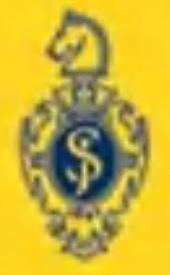
\includegraphics[max width=\textwidth]{2025_06_06_fac2836a92464059da43g-001}
\end{center}

Springer 版权所有

\begin{center}
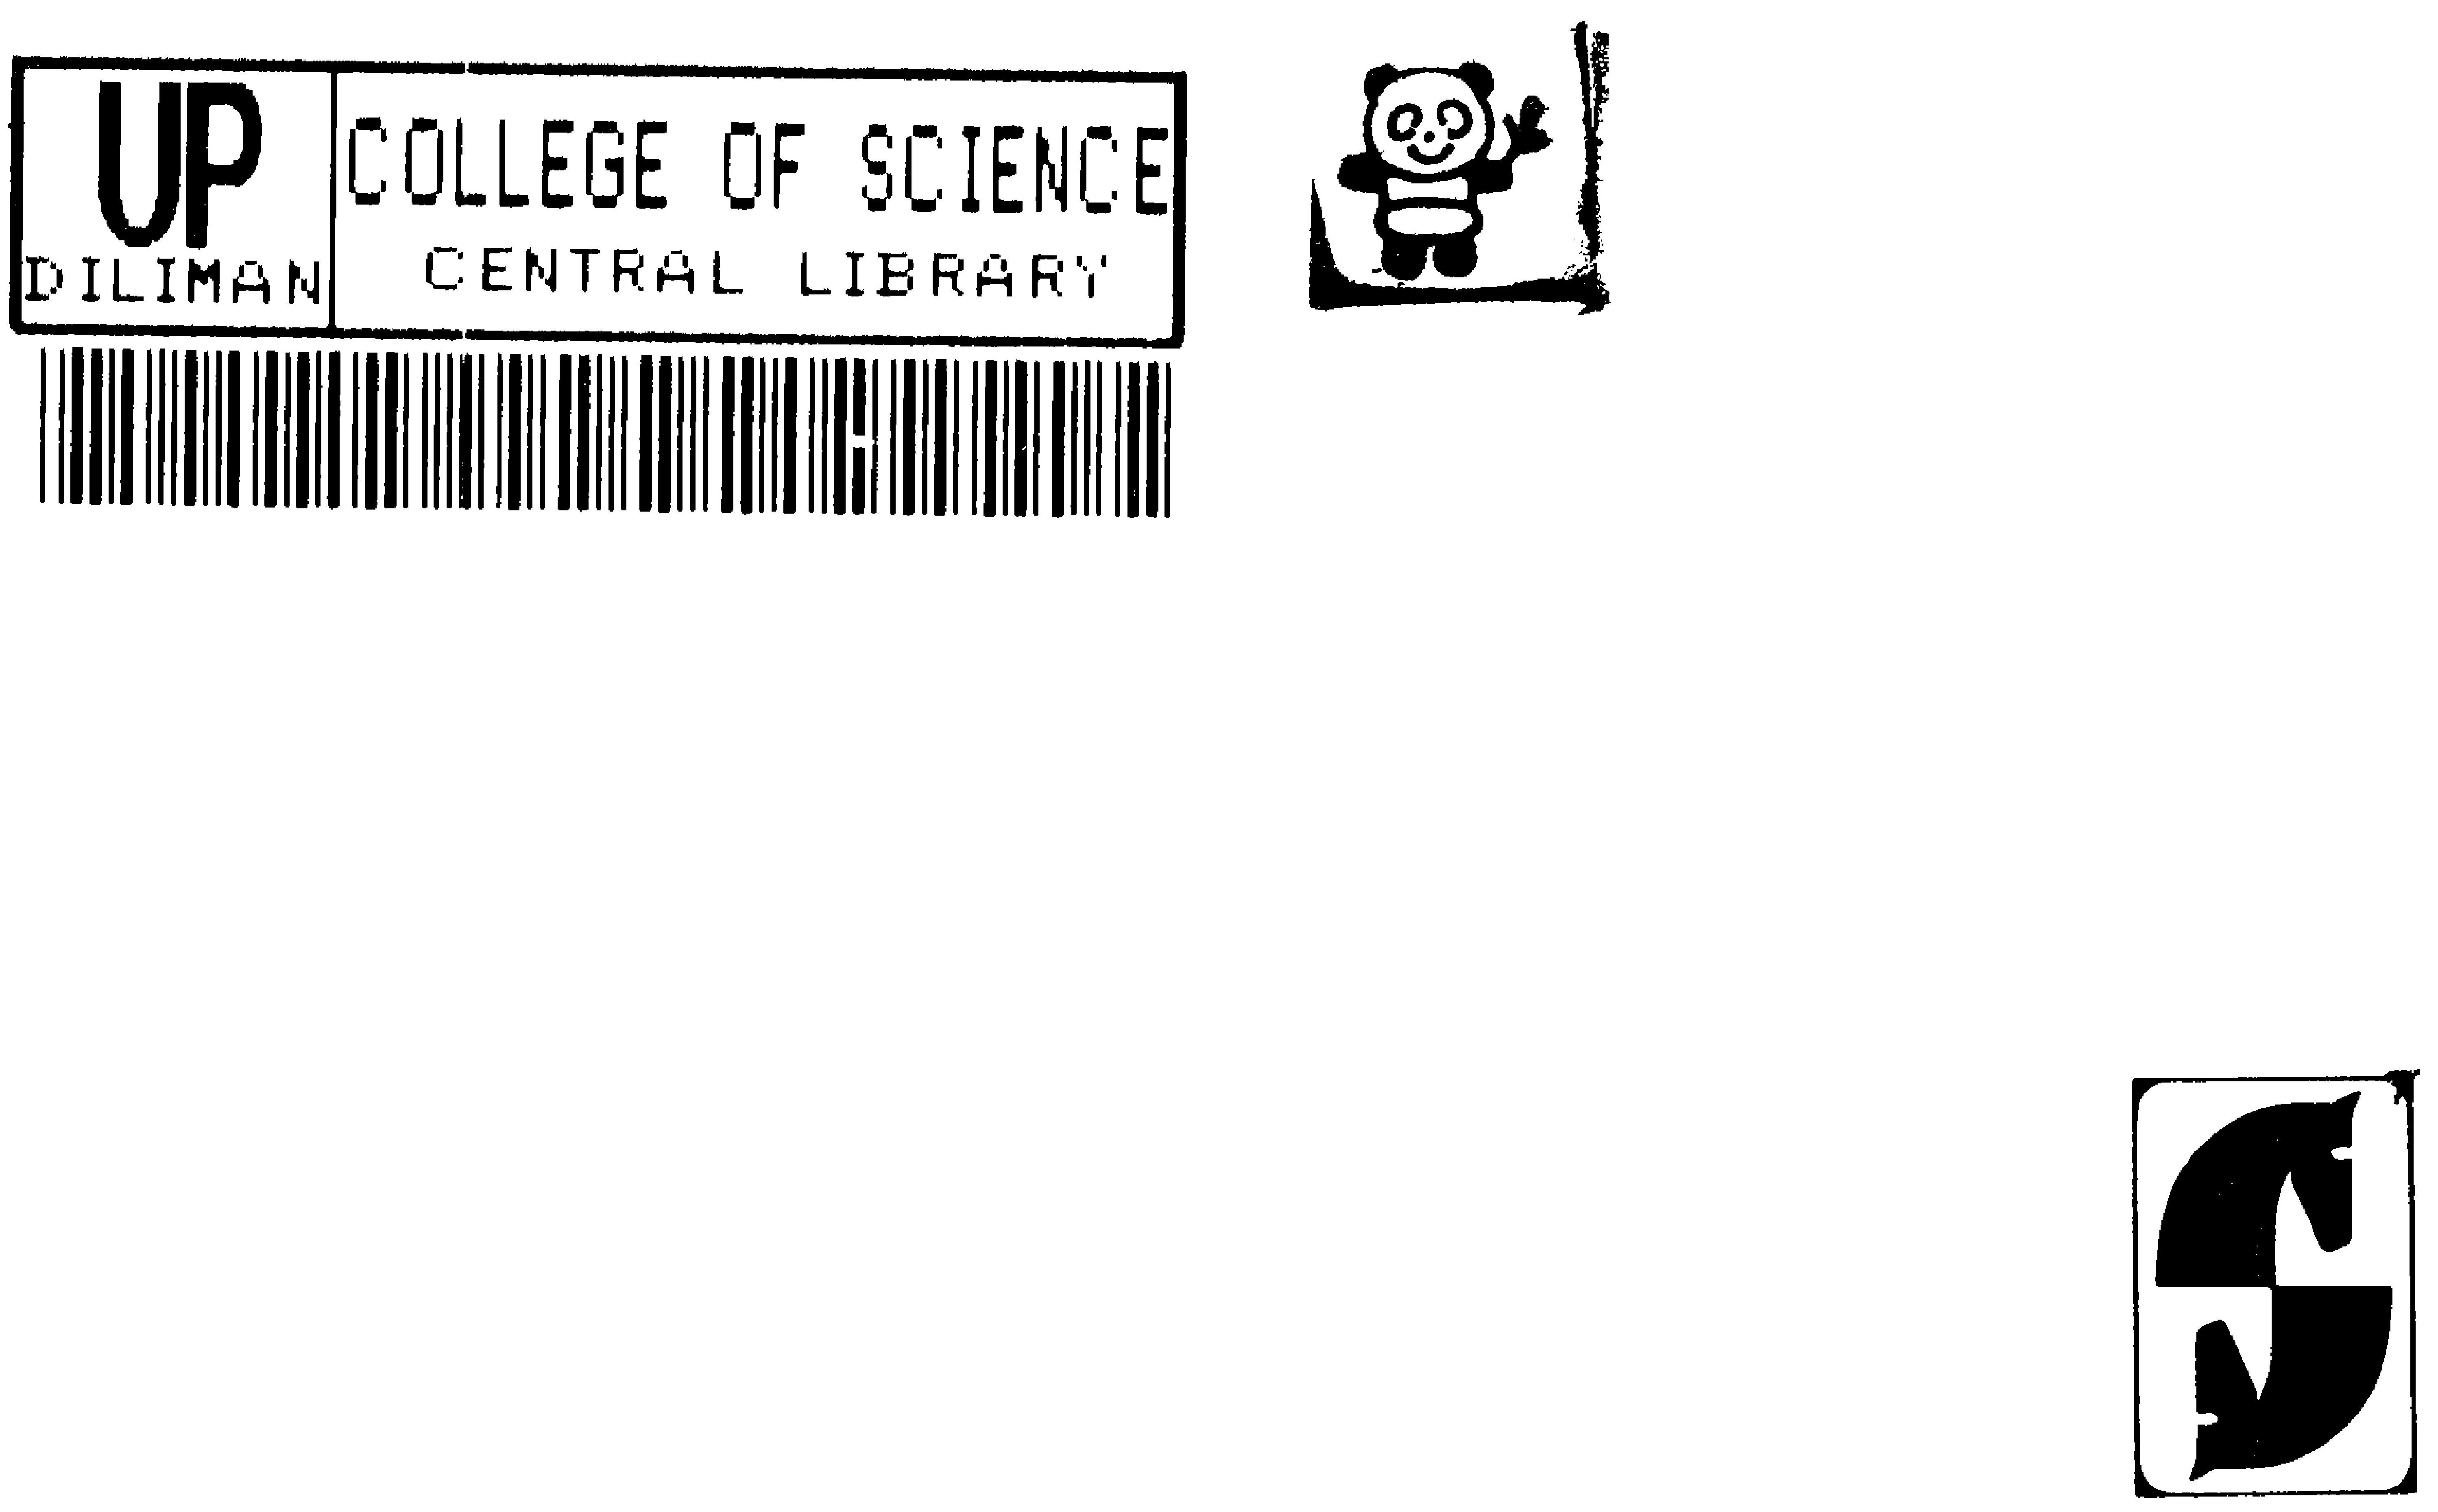
\includegraphics[max width=\textwidth]{2025_06_06_fac2836a92464059da43g-002}
\end{center}

Professor of Mathematics\\
University of Massachusetts\\
Amherst, MA 01003

AMS Subject Classification (1970)\\
17 B XX, 20 G 05, 22 E 60

All rights reserved.\\
No part of this book may be translated or reproduced in any form without written permission from Springer-Verlag.\\
© 1972 by Springer-Verlag New York Inc.\\
Library of Congress Catalog Card Number 72-85951\\
Printed in the United States of America.\\
987654\\
Third printing, revised, 1980.\\
ISBN 0-387-90052-7 Springer-Verlag New York •Heidelberg • Berlin (soft cover)\\
ISBN 0-387-90053-5 Springer-Verlag New York •Heidelberg • Berlin (hard cover)\\
ISBN 3-540-90052-7 Springer-Verlag Berlin $\cdot$ Heidelberg $\cdot$ New York (soft cover)\\
ISBN 3-540-90053-5 Springer-Verlag Berlin $\cdot$ Heidelberg $\cdot$ New York (hard cover)

To the memory of my nephews Willard Charles Humphreys III and

Thomas Edward Humphreys

\section*{Preface}
This book is designed to introduce the reader to the theory of semisimple Lie algebras over an algebraically closed field of characteristic 0 , with emphasis on representations. A good knowledge of linear algebra (including eigenvalues, bilinear forms, euclidean spaces, and tensor products of vector spaces) is presupposed, as well as some acquaintance with the methods of abstract algebra. The first four chapters might well be read by a bright undergraduate; however, the remaining three chapters are admittedly a little more demanding.

Besides being useful in many parts of mathematics and physics, the theory of semisimple Lie algebras is inherently attractive, combining as it does a certain amount of depth and a satisfying degree of completeness in its basic results. Since Jacobson's book appeared a decade ago, improvements have been made even in the classical parts of the theory. I have tried to incorporate some of them here and to provide easier access to the subject for non-specialists. For the specialist, the following features should be noted:\\
(1) The Jordan-Chevalley decomposition of linear transformations is emphasized, with "toral" subalgebras replacing the more traditional Cartan subalgebras in the semisimple case.\\
(2) The conjugacy theorem for Cartan subalgebras is proved (following D. J. Winter and G. D. Mostow) by elementary Lie algebra methods, avoiding the use of algebraic geometry.\\
(3) The isomorphism theorem is proved first in an elementary way (Theorem 14.2), but later obtained again as a corollary of Serre's Theorem (18.3), which gives a presentation by generators and relations.\\
(4) From the outset, the simple algebras of types $A, B, C, D$ are emphasized in the text and exercises.\\
(5) Root systems are treated axiomatically (Chapter III), along with some of the theory of weights.\\
(6) A conceptual approach to Weyl's character formula, based on Harish-Chandra's theory of "characters" and independent of Freudenthal's multiplicity formula (22.3), is presented in §23 and §24. This is inspired by D.-N. Verma's thesis, and recent work of I. N. Bernstein, I. M. Gel'fand, S. I. Gel'fand.\\
(7) The basic constructions in the theory of Chevalley groups are given in Chapter VII, following lecture notes of R. Steinberg.

I have had to omit many standard topics (most of which I feel are better suited to a second course), e.g., cohomology, theorems of Levi and Mal'cev, theorems of Ado and Iwasawa, classification over non-algebraically closed fields, Lie algebras in prime characteristic. I hope the reader will be stimulated to pursue these topics in the books and articles listed under References, especially Jacobson [1], Bourbaki [1], [2], Winter [1], Seligman [1].

A few words about mechanics: Terminology is mostly traditional, and notation has been kept to a minimum, to facilitate skipping back and forth in the text. After Chapters I-III, the remaining chapters can be read in almost any order if the reader is willing to follow up a few references (except that VII depends on $\S 20$ and $\S 21$, while VI depends on $\S 17$ ). A reference to Theorem 14.2 indicates the (unique) theorem in subsection 14.2 (of §14). Notes following some sections indicate nonstandard sources or further reading, but I have not tried to give a history of each theorem (for historical remarks, cf. Bourbaki [2] and Freudenthal-deVries [1]). The reference list consists largely of items mentioned explicitly; for more extensive bibliographies, consult Jacobson [1], Seligman [1]. Some 240 exercises, of all shades of difficulty, have been included; a few of the easier ones are needed in the text.

This text grew out of lectures which I gave at the N.S.F. Advanced Science Seminar on Algebraic Groups at Bowdoin College in 1968; my intention then was to enlarge on J.-P. Serre's excellent but incomplete lecture notes [2]. My other literary debts (to the books and lecture notes of N. Bourbaki, N. Jacobson, R. Steinberg, D. J. Winter, and others) will be obvious. Less obvious is my personal debt to my teachers, George Seligman and Nathan Jacobson, who first aroused my interest in Lie algebras. I am grateful to David J. Winter for giving me pre-publication access to his book, to Robert L. Wilson for making many helpful criticisms of an earlier version of the manuscript, to Connie Engle for her help in preparing the final manuscript, and to Michael J. DeRise for moral support. Financial assistance from the Courant Institute of Mathematical Sciences and the National Science Foundation is also gratefully acknowledged.

New York, April 4, 1972



\section*{Preface to the Second Printing}
In addition to correcting minor errors and improving a few arguments, I have taken this opportunity to add an appendix to §24, in which Weyl's formula is obtained more efficiently (avoiding the use of §23). I want to thank those who have pointed out errors and suggested helpful alternatives, in particular: J. Carr, J. Dorfmeister, M. Eichler, M. Elmer, K. W. Gruenberg, J. H. Lindsey, B. Weisfeiler, R. L. Wilson.

\section*{Notation and Conventions}
$\mathbf{Z}, \mathbf{Z}^{+}, \mathbf{Q}, \mathbf{R}, \mathbf{C}$ denote (respectively) the integers, nonnegative integers, rationals, reals, and complex numbers\\
$\amalg$ denotes direct sum of vector spaces\\
$A \triangleright B$ denotes the semidirect product of groups $A$ and $B$, with $B$ normal\\
Card $=$ cardinality $\quad$ Ker $=$ kernel\\
char = characteristic $\quad$ Im = image\\
det $=$ determinant $\quad \operatorname{Tr}=$ trace\\
$\operatorname{dim}=$ dimension

\section*{Table of Contents}
PREFACE. ..... vii\\
I. BASIC CONCEPTS ..... 1

\begin{enumerate}
  \item Definitions and first examples ..... 1\\
1.1 The notion of Lie algebra ..... 1\\
1.2 Linear Lie algebras ..... 2\\
1.3 Lie algebras of derivations ..... 4\\
1.4 Abstract Lie algebras ..... 4
  \item Ideals and homomorphisms ..... 6\\
2.1 Ideals ..... 6\\
2.2 Homomorphisms and representations ..... 7\\
2.3 Automorphisms ..... 8
  \item Solvable and nilpotent Lie algebras ..... 10\\
3.1 Solvability ..... 10\\
3.2 Nilpotency ..... 11\\
3.3 Proof of Engel's Theorem ..... 12\\
II. SEMISIMPLE LIE ALGEBRAS ..... 15
  \item Theorems of Lie and Cartan ..... 15\\
4.1 Lie's Theorem ..... 15\\
4.2 Jordan-Chevalley decomposition ..... 17\\
4.3 Cartan's Criterion. ..... 19
  \item Killing form . ..... 21\\
5.1 Criterion for semisimplicity ..... 21\\
5.2 Simple ideals of L. ..... 22\\
5.3 Inner derivations ..... 23\\
5.4 Abstract Jordan decomposition ..... 24
  \item Complete reducibility of representations ..... 25\\
6.1 Modules ..... 25\\
6.2 Casimir element of a representation ..... 27\\
6.3 Weyl's Theorem ..... 28\\
6.4 Preservation of Jordan decomposition ..... 29
  \item Representations of $\mathfrak{s l}(2, \mathrm{~F})$ ..... 31\\
7.1 Weights and maximal vectors. ..... 31\\
7.2 Classification of irreducible modules ..... 32
  \item Root space decomposition ..... 35\\
8.1 Maximal toral subalgebras and roots ..... 35\\
8.2 Centralizer of $H$ ..... 36\\
8.3 Orthogonality properties ..... 37\\
8.4 Integrality properties ..... 38\\
8.5 Rationality properties. Summary ..... 39\\
III. ROOT SYSTEMS ..... 42
  \item Axiomatics ..... 42\\
9.1 Reflections in a euclidean space ..... 42\\
9.2 Root systems ..... 42\\
9.3 Examples ..... 43\\
9.4 Pairs of roots ..... 44
  \item Simple roots and Weyl group ..... 47\\
10.1 Bases and Weyl chambers ..... 47\\
10.2 Lemmas on simple roots ..... 50\\
10.3 The Weyl group ..... 51\\
10.4 Irreducible root systems ..... 52
  \item Classification ..... 55\\
11.1 Cartan matrix of $\Phi$ ..... 55\\
11.2 Coxeter graphs and Dynkin diagrams ..... 56\\
11.3 Irreducible components ..... 57\\
11.4 Classification theorem ..... 57
  \item Construction of root systems and automorphisms ..... 63\\
12.1 Construction of types A-G ..... 63\\
12.2 Automorphisms of $\Phi$ ..... 65
  \item Abstract theory of weights ..... 67\\
13.1 Weights ..... 67\\
13.2 Dominant weights ..... 68\\
13.3 The weight $\delta$ ..... 70\\
13.4 Saturated sets of weights ..... 70\\
IV. ISOMORPHISM AND CONJUGACY THEOREMS ..... 73
  \item Isomorphism theorem ..... 73\\
14.1 Reduction to the simple case ..... 73\\
14.2 Isomorphism theorem ..... 74\\
14.3 Automorphisms ..... 76
  \item Cartan subalgebras ..... 78\\
15.1 Decomposition of $L$ relative to ad $x$ ..... 78\\
15.2 Engel subalgebras ..... 79\\
15.3 Cartan subalgebras ..... 80\\
15.4 Functorial properties ..... 81
  \item Conjugacy theorems ..... 81\\
16.1 The group $\mathscr{E}(L)$ ..... 82\\
16.2 Conjugacy of CSA's (solvable case) ..... 82\\
16.3 Borel subalgebras ..... 83\\
16.4 Conjugacy of Borel subalgebras ..... 84\\
16.5 Automorphism groups ..... 87\\
V. EXISTENCE THEOREM ..... 89
  \item Universal enveloping algebras ..... 89\\
17.1 Tensor and symmetric algebras ..... 89\\
17.2 Construction of $\mathfrak{U}(L)$ ..... 90\\
17.3 PBW Theorem and consequences ..... 91\\
17.4 Proof of PBW Theorem ..... 93\\
Table of Contents ..... xi\\
17.5 Free Lie algebras ..... 94
  \item Generators and relations ..... 95\\
18.1 Relations satisfied by $L$. ..... 96\\
18.2 Consequences of (S1)-(S3) ..... 96\\
18.3 Serre's Theorem ..... 98\\
18.4 Application: Existence and uniqueness theorems ..... 101
  \item The simple algebras ..... 102\\
19.1 Criterion for semisimplicity ..... 102\\
19.2 The classical algebras ..... 102\\
19.3 The algebra $\mathrm{G}_{2}$ ..... 103\\
VI. REPRESENTATION THEORY ..... 107
  \item Weights and maximal vectors ..... 107\\
20.1 Weight spaces ..... 107\\
20.2 Standard cyclic modules ..... 108\\
20.3 Existence and uniqueness theorems ..... 109
  \item Finite dimensional modules ..... 112\\
21.1 Necessary condition for finite dimension ..... 112\\
21.2 Sufficient condition for finite dimension ..... 113\\
21.3 Weight strings and weight diagrams ..... 114\\
21.4 Generators and relations for $V(\lambda)$ ..... 115
  \item Multiplicity formula ..... 117\\
22.1 A universal Casimir element ..... 118\\
22.2 Traces on weight spaces ..... 119\\
22.3 Freudenthal's formula ..... 121\\
22.4 Examples ..... 123\\
22.5 Formal characters. ..... 124
  \item Characters ..... 126\\
23.1 Invariant polynomial functions ..... 126\\
23.2 Standard cyclic modules and characters ..... 128\\
23.3 Harish-Chandra's Theorem ..... 130\\
Appendix ..... 132
  \item Formulas of Weyl, Kostant, and Steinberg ..... 135\\
24.1 Some functions on $H^{*}$ ..... 135\\
24.2 Kostant's multiplicity formula ..... 136\\
24.3 Weyl's formulas ..... 138\\
24.4 Steinberg's formula ..... 140\\
Appendix ..... 143\\
VII. CHEVALLEY ALGEBRAS AND GROUPS ..... 145
  \item Chevalley basis of $L$ ..... 145\\
25.1 Pairs of roots ..... 145\\
25.2 Existence of a Chevalley basis ..... 145\\
25.3 Uniqueness questions ..... 146\\
25.4 Reduction modulo a prime ..... 148\\
25.5 Construction of Chevalley groups (adjoint type) ..... 149
  \item Kostant's Theorem ..... 151\\
26.1 A combinatorial lemma ..... 152\\
26.2 Special case: sl (2, F) ..... 153\\
26.3 Lemmas on commutation ..... 154\\
26.4 Proof of Kostant's Theorem ..... 156
  \item Admissible lattices . ..... 157\\
27.1 Existence of admissible lattices ..... 157\\
27.2 Stabilizer of an admissible lattice ..... 159\\
27.3 Variation of admissible lattice ..... 161\\
27.4 Passage to an arbitrary field ..... 162\\
27.5 Survey of related results ..... 163\\
References ..... 165\\
Index of Terminology ..... 167\\
Index of Symbols ..... 170
\end{enumerate}

\section*{Introduction to Lie Algebras and Representation Theory}
\section*{Chapter I}
\section*{Basic Concepts}
In this chapter F denotes an arbitrary (commutative) field.

\section*{1. Definitions and first examples}
\subsection*{1.1. The notion of Lie algebra}
Lie algebras arise "in nature" as vector spaces of linear transformations endowed with a new operation which is in general neither commutative nor associative: $[x, y]=x y-y x$ (where the operations on the right side are the usual ones). It is possible to describe this kind of system abstractly in a few axioms.

Definition. A vector space $L$ over a field F , with an operation $L \times L \rightarrow L$, denoted $(x, y) \mapsto[x y]$ and called the bracket or commutator of $x$ and $y$, is called a Lie algebra over F if the following axioms are satisfied:\\
(L1) The bracket operation is bilinear.\\
(L2) $[x x]=0$ for all $x$ in $L$.\\
(L3) $[x[y z]]+[y[z x]]+[z[x y]]=0 \quad(x, y, z \in L)$.\\
Axiom (L3) is called the Jacobi identity. Notice that (L1) and (L2), applied to $[x+y, x+y]$, imply anticommutativity: $\left(L 2^{\prime}\right)[x y]=-[y x]$. (Conversely, if char $\mathrm{F} \neq 2$, it is clear that ( $L 2$ ') will imply ( $L 2$ ).)

We say that two Lie algebras $L, L^{\prime}$ over F are isomorphic if there exists a vector space isomorphism $\phi: L \rightarrow L^{\prime}$ satisfying $\phi([x y])=[\phi(x) \phi(y)]$ for all $x, y$ in $L$ (and then $\phi$ is called an isomorphism of Lie algebras). Similarly, it is obvious how to define the notion of (Lie) subalgebra of $L$ : A subspace $K$ of $L$ is called a subalgebra if $[x y] \in K$ whenever $x, y \in K$; in particular, $K$ is a Lie algebra in its own right relative to the inherited operations. Note that any nonzero element $x \in L$ defines a one dimensional subalgebra $\mathrm{F} x$, with trivial multiplication, because of (L2).

In this book we shall be concerned almost exclusively with Lie algebras $L$ whose underlying vector space is finite dimensional over F. This will always be assumed, unless otherwise stated. We hasten to point out, however, that certain infinite dimensional vector spaces and associative algebras over $F$ will play a vital role in the study of representations (Chapters V-VII). We also mention, before looking at some concrete examples, that the axioms for a Lie algebra make perfectly good sense if $L$ is only assumed to be a module over a commutative ring, but we shall not pursue this point of view here.

\subsection*{1.2. Linear Lie algebras}
If $V$ is a finite dimensional vector space over F , denote by End $V$ the set of linear transformations $V \rightarrow V$. As a vector space over F, End $V$ has dimension $n^{2}(n=\operatorname{dim} V)$, and End $V$ is a ring relative to the usual product operation. Define a new operation $[x, y]=x y-y x$, called the bracket of $x$ and $y$. With this operation End $V$ becomes a Lie algebra over F: axioms (L1) and (L2) are immediate, while (L3) requires a brief calculation (which the reader is urged to carry out at this point). In order to distinguish this new algebra structure from the old associative one, we write $\mathfrak{g l}(V)$ for End $V$ viewed as Lie algebra and call it the general linear algebra (because it is closely associated with the general linear group $G L(V)$ consisting of all invertible endomorphisms of $V$ ). When $V$ is infinite dimensional, we shall also use the notation $\mathfrak{g l}(V)$ without further comment.

Any subalgebra of a Lie algebra $\mathfrak{g l}(V)$ is called a linear Lie algebra. The reader who finds matrices more congenial than linear transformations may prefer to fix a basis for $V$, thereby identifying $\mathfrak{g l}(V)$ with the set of all $n \times n$ matrices over F , denoted $\mathrm{gl}(n, \mathrm{~F})$. This procedure is harmless, and very convenient for making explicit calculations. For reference, we write down the multiplication table for $\mathfrak{g l}(n, \mathrm{~F})$ relative to the standard basis consisting of the matrices $e_{i j}$ (having 1 in the $(i, j)$ position and 0 elsewhere). Since $e_{i j} e_{k l}=\delta_{j k} e_{i l}$, it follows that:


\begin{equation*}
\left[e_{i j}, e_{k l}\right]=\delta_{j k} e_{i l}-\delta_{l i} e_{k j} \tag{*}
\end{equation*}


Notice that the coefficients are all $\pm 1$ or 0 ; in particular, all of them lie in the prime field of F.

Now for some further examples, which are central to the theory we are going to develop in this book. They fall into four families $A_{\ell}, B_{\ell}, C_{\ell}, D_{\ell}$ $(\ell \geq 1)$ and are called the classical algebras (because they correspond to certain of the classical linear Lie groups).\\
$\mathrm{A}_{\ell}:$ Let $\operatorname{dim} V=\ell+1$. Denote by $\mathfrak{s l}(V)$, or $\mathfrak{s l}(\ell+1, \mathrm{~F})$, the set of endomorphisms of $V$ having trace zero. (Recall that the trace of a matrix is the sum of its diagonal entries; this is independent of choice of basis for $V$, hence makes sense for an endomorphism of $V$.) Since $\operatorname{Tr}(x y)=\operatorname{Tr}(y x)$, and $\operatorname{Tr}(x+y)=\operatorname{Tr}(x)+\operatorname{Tr}(y), \mathfrak{s l}(V)$ is a subalgebra of $\mathfrak{g l}(V)$, called the special linear algebra because of its connection with the special linear group $S L(V)$ of endomorphisms of det 1 . What is its dimension? On the one hand $\mathfrak{s l}(V)$ is a proper subalgebra of $\mathfrak{g l}(V)$, hence of dimension at most $(\ell+1)^{2}-1$. On the other hand, we can exhibit this number of linearly independent matrices of trace zero: Take all $e_{i j}(i \neq j)$, along with all $h_{i}=e_{i i}-e_{i+1, i+1}$ $(1 \leq i \leq \ell)$, for a total of $\ell+(\ell+1)^{2}-(\ell+1)$ matrices. We shall always view this as the standard basis for $\mathfrak{s l}(\ell+1, \mathrm{~F})$.\\
$\mathrm{C}_{\ell}$ : Let $\operatorname{dim} V=2 \ell$, with basis $\left(v_{1}, \ldots, v_{2 \ell}\right)$. Define a nondegenerate skew-symmetric form $f$ on $V$ by the matrix $s=\left(\begin{array}{rr}0 & I_{\ell} \\ -I_{\ell} & 0\end{array}\right)$. (It can be shown\\
that even dimensionality is a necessary condition for existence of a nondegenerate bilinear form satisfying $f(v, w)=-f(w, v)$.) Denote by $\mathfrak{s p}(V)$, or $\mathfrak{s p}(2 \ell, \mathfrak{F})$, the symplectic algebra, which by definition consists of all endomorphisms $x$ of $V$ satisfying $f(x(v), w)=-f(v, x(w))$. The reader can easily verify that $\mathfrak{s p}(V)$ is closed under the bracket operation. In matrix terms, the condition for $x=\left(\begin{array}{cc}m & n \\ p & q\end{array}\right)(m, n, p, q \in \mathfrak{g l}(\ell, \mathrm{~F}))$ to be symplectic is that $s x=-x^{t} s\left(x^{t}=\right.$ transpose of $\left.x\right)$, i.e., that $n^{t}=n, p^{t}=p$, and $m^{t}=-q$. (This last condition forces $\operatorname{Tr}(x)=0$.) It is easy now to compute a basis for $\mathfrak{s p}(2 \ell, \mathrm{~F})$. Take the diagonal matrices $e_{i i}-e_{\ell+i, \ell+i}(1 \leq i \leq \ell)$, $\ell$ in all. Add to these all $e_{i j}-e_{\ell+j, \ell+i}(1 \leq i \neq j \leq \ell), \ell^{2}-\ell$ in number. For $n$ we use the matrices $e_{i, \ell+i}(1 \leq i \leq \ell)$ and $e_{i, \ell+j}+e_{j, \ell+i}(1 \leq i<j$ $\leq \ell$ ), a total of $\ell+\frac{1}{2} \ell(\ell-1)$, and similarly for the positions in $p$. Adding up, we find $\operatorname{dim} \mathfrak{s p}(2 \ell, \mathrm{~F})=2 \ell^{2}+\ell$.\\
$\mathrm{B}_{\ell}:$ Let $\operatorname{dim} V=2 \ell+1$ be odd, and take $f$ to be the nondegenerate symmetric bilinear form on $V$ whose matrix is $s=\left(\begin{array}{ccc}1 & 0 & 0 \\ 0 & 0 & I_{\ell} \\ 0 & I_{\ell} & 0\end{array}\right)$. The orthogonal algebra $\mathfrak{D}(V)$, or $\mathfrak{D}(2 \ell+1, \mathfrak{F})$, consists of all endomorphisms of $V$ satisfying $f(x(v), w)=-f(v, x(w))$ (the same requirement as for $\mathrm{C}_{\ell}$ ). If we partition $x$ in the same form as $s$, say $x=\left(\begin{array}{lll}a & b_{1} & b_{2} \\ c_{1} & m & n \\ c_{2} & p & q\end{array}\right)$, then the condition $s x=-x^{t} s$ translates into the following set of conditions: $a=0, c_{1}=-b_{2}^{t}, c_{2}=-b_{1}^{t}$, $q=-m^{t}, n^{t}=-n, p^{t}=-p$. (As in the case of $\mathrm{C}_{\ell}$, this shows that $\operatorname{Tr}(x)$ $=0$.) For a basis, take first the $\ell$ diagonal matrices $e_{i i}-e_{\ell+i, \ell+i}(2 \leq i \leq$ $\ell+1)$. Add the $2 \ell$ matrices involving only row one and column one: $e_{1, \ell+i+1}-e_{i+1,1}$ and $e_{1, i+1}-e_{\ell+i+1,1} \quad(1 \leq i \leq \ell)$. Corresponding to $q=-m^{t}$, take (as for $\mathrm{C}_{\ell}$ ) $e_{i+1, j+1}-e_{\ell+j+1, \ell+i+1}(1 \leq i \neq j \leq \ell)$. For $n$ take $e_{i+1, \ell+j+1}-e_{j+1, \ell+i+1}(1 \leq i<j \leq \ell)$, and for $p, e_{i+\ell+1, j+1}-$ $e_{j+\ell+1, i+1}(1 \leq j<i \leq \ell)$. The total number of basis elements is $2 \ell^{2}+\ell$ (notice that this was also the dimension of $\mathrm{C}_{\ell}$ ).\\
$\mathrm{D}_{\ell}$ : Here we obtain another orthogonal algebra. The construction is identical to that for $\mathrm{B}_{\ell}$, except that $\operatorname{dim} V=2 \ell$ is even and $s$ has the simpler form $\left(\begin{array}{cc}0 & I_{\ell} \\ I_{\ell} & 0\end{array}\right)$. We leave it as an exercise for the reader to construct a basis and to verify that $\operatorname{dim} \mathfrak{o}(2 \ell, \mathrm{~F})=2 \ell^{2}-\ell$ (Exercise 8).

We conclude this subsection by mentioning several other subalgebras of $\mathfrak{g l}(n, \mathrm{~F})$ which play an important subsidiary role for us. Let $\mathrm{t}(n, \mathrm{~F})$ be the set of upper triangular matrices $\left(a_{i j}\right), a_{i j}=0$ if $i>j$. Let $\mathfrak{n}(n$, F $)$ be the strictly upper triangular matrices ( $a_{t j}=0$ if $i \geq j$ ). Finally, let $\mathfrak{d}(n, F)$ be the set of all diagonal matrices. It is trivial to check that each of these is closed under the bracket. Notice also that $\mathrm{t}(n, \mathrm{~F})=\mathfrak{d}(n, \mathrm{~F})+\mathfrak{n}(n, \mathrm{~F})$ (vector space direct sum), with $[\mathfrak{d}(n, \mathcal{F}), \mathfrak{n}(n, \mathcal{F})]=\mathfrak{n}(n, \mathcal{F})$, hence $[\mathfrak{t}(n, \mathcal{F}), \mathfrak{t}(n, \mathcal{F})]=\mathfrak{n}(n, \mathcal{F})$, cf. Exercise 5. (If $H, K$ are subalgebras of $L,[H K]$ denotes the subspace of $L$ spanned by commutators $[x y], x \in H, y \in K$.)

\subsection*{1.3. Lie algebras of derivations}
Some Lie algebras of linear transformations arise most naturally as derivations of algebras. By an F-algebra (not necessarily associative) we simply mean a vector space $\mathfrak{A}$ over $F$ endowed with a bilinear operation $\mathfrak{A} \times \mathfrak{U} \rightarrow \mathfrak{I}$. usually denoted by juxtaposition (unless $\mathfrak{A}$ is a Lie algebra, in which case we always use the bracket). By a derivation of $\mathfrak{A}$ we mean a linear map $\delta: \mathfrak{U} \rightarrow \mathfrak{U}$ satisfying the familiar product rule $\delta(a b)=a \delta(b)+\delta(a) b$. It is easil checked that the collection Der $\mathfrak{A}$ of all derivations of $\mathfrak{A}$ is a vector subspace of End $\mathfrak{A}$. The reader should also verify that the commutator [ $\delta . \delta^{\prime}$ ] of two derivations is again a derivation (though the ordinary product need not be, cf. Exercise 11). So Der $\mathfrak{A}$ is a subalgebra of $\mathfrak{g l}(\mathfrak{A})$.

Since a Lie algebra $L$ is an F-algebra in the above sense, Der $L$ is defined. Certain derivations arise quite naturally, as follows. If $x \in L, y \mapsto[x y]$ is an endomorphism of $L$, which we denote ad $x$. In fact, ad $x \in \operatorname{Der} L$, because we can rewrite the Jacobi identity (using ( $L 2^{\prime}$ )) in the form: $[x[y z]]=[[x y] z]$ $+[y[x z]]$. Derivations of this form are called inner, all others outer. It is of course perfectly possible to have ad $x=0$ even when $x \neq 0$ : this occurs in any one dimensional Lie algebra, for example. The map $L \rightarrow$ Der $L$ sending $x$ to ad $x$ is called the adjoint representation of $L$; it plays a decisive role in all that follows.

Sometimes we have occasion to view $x$ simultaneously as an element of $L$ and of a subalgebra $K$ of $L$. To avoid ambiguity, the notation $\operatorname{ad}_{\mathrm{L}} x$ or $\operatorname{ad}_{\mathrm{K}} x$ will be used to indicate that $x$ is acting on $L$ (respectively, $K$ ). For example, if $x$ is a diagonal matrix, then $\operatorname{ad}_{\mathfrak{d}(n, \mathrm{~F})}(x)=0$, whereas $\operatorname{ad}_{\mathfrak{g l}(n, \mathrm{~F})}(x)$ need not be zero.

\subsection*{1.4. Abstract Lie algebras}
We have looked at some natural examples of linear Lie algebras. It is known that, in fact, every (finite dimensional) Lie algebra is isomorphic to some linear Lie algebra (theorems of Ado, Iwasawa). This will not be proved here (cf. Jacobson [1] Chapter VI, or Bourbaki [1]); however, it will be obvious at an early stage of the theory that the result is true for all cases we are interested in.

Sometimes it is desirable, however, to contemplate Lie algebras abstractly. For example, if $L$ is an arbitrary finite dimensional vector space over $F$, we can view $L$ as a Lie algebra by setting $[x y]=0$ for all $x, y \in L$. Such an algebra, having trivial Lie multiplication, is called abelian (because in the linear case $[x, y]=0$ just means that $x$ and $y$ commute). If $L$ is any Lie algebra, with basis $x_{1}, \ldots, x_{n}$ it is clear that the entire multiplication table of $L$ can be recovered from the structure constants $a_{i j}^{k}$ which occur in the expressions $\left[x_{i} x_{j}\right]=\sum_{k=1}^{n} a_{i j}^{k} x_{k}$. Those for which $i \geq j$ can even be deduced from the others, thanks to ( $L 2$ ), ( $L 2$ ). Turning this remark around, it is possible to define an abstract Lie algebra from scratch simply by specifying\\
a set of structure constants. Naturally, not just any set of scalars $\left\{a_{i j}^{k}\right\}$ will do, but a moment's thought shows that it is enough to require the "obvious" identities, those implied by (L2) and (L3):

$$
\begin{gathered}
a_{i i}^{k}=0=a_{i j}^{k}+a_{j i}^{k} \\
\sum_{k}\left(a_{i j}^{k} a_{k \ell}^{m}+a_{j \ell}^{k} a_{k i}^{m}+a_{\ell i}^{k} a_{k j}^{m}\right)=0
\end{gathered}
$$

In practice, we shall have no occasion to construct Lie algebras in this artificial way. But, as an application of the abstract point of view, we can determine (up to isomorphism) all Lie algebras of dimension $\leq 2$. In dimension 1 there is a single basis vector $x$, with multiplication table $[x x]=0(L 2)$. In dimension 2, start with a basis $x, y$ of $L$. Clearly, all products in $L$ yield scalar multiples of $[x y]$. If these are all 0 , then $L$ is abelian. Otherwise, we can replace $x$ in the basis by a vector spanning the one dimensional space of multiples of the original [ $x y$ ], and take $y$ to be any other vector independent of the new $x$. Then $[x y]=a x(a \neq 0)$. Replacing $y$ by $a^{-1} y$, we finally get $[x y]=x$. Abstractly, therefore, at most one nonabelian $L$ exists (the reader should check that $[x y]=x$ actually defines a Lie algebra).

\section*{Exercises}
\begin{enumerate}
  \item Let $L$ be the real vector space $\mathbf{R}^{3}$. Define $[x y]=x \times y$ (cross product of vectors) for $x, y \in L$, and verify that $L$ is a Lie algebra. Write down the structure constants relative to the usual basis of $\mathbf{R}^{3}$.
  \item Verify that the following equations and those implied by (L1) (L2) define a Lie algebra structure on a three dimensional vector space with basis $(x, y, z):[x y]=z,[x z]=y,[y z]=0$.
  \item Let $x=\left(\begin{array}{ll}0 & 1 \\ 0 & 0\end{array}\right), h=\left(\begin{array}{rr}1 & 0 \\ 0 & -1\end{array}\right), y=\left(\begin{array}{ll}0 & 0 \\ 1 & 0\end{array}\right)$ be an ordered basis for $\mathfrak{s l}(2, \mathrm{~F})$. Compute the matrices of ad $x$, ad $h$, ad $y$ relative to this basis.
  \item Find a linear Lie algebra isomorphic to the nonabelian two dimensional algebra constructed in (1.4). [Hint: Look at the adjoint representation.]
  \item Verify the assertions made in (1.2) about $\mathfrak{t}(n, \mathcal{F}), \mathfrak{d}(n, \mathcal{F}), \mathfrak{n}(n, \mathcal{F})$, and compute the dimension of each algebra, by exhibiting bases.
  \item Let $x \in \mathfrak{g l}(n, \mathrm{~F})$ have $n$ distinct eigenvalues $a_{1}, \ldots, a_{n}$ in F. Prove that the eigenvalues of ad $x$ are precisely the $n^{2}$ scalars $a_{i}-a_{j}(1 \leq i, j \leq n)$, which of course need not be distinct.
  \item Let $\mathfrak{s}(n, \mathrm{~F})$ denote the scalar matrices (= scalar multiples of the identity) in $\mathfrak{g l}(n, \mathcal{F})$. If char $\mathcal{F}$ is 0 or else a prime not dividing $n$, prove that $\mathfrak{g l}(n, \mathrm{~F})=\mathfrak{s l}(n, \mathrm{~F})+\mathfrak{s}(n, \mathrm{~F})$ (direct sum of vector spaces), with $[\mathfrak{s}(n, \mathrm{~F})$, $g[(n, F)]=0$.
  \item Verify the stated dimension of $D_{\ell}$.
  \item When char $\mathrm{F}=0$, show that each classical algebra $L=\mathrm{A}_{\ell}, \mathrm{B}_{\ell}, \mathrm{C}_{\ell}$, or $\mathrm{D}_{\ell}$ is equal to $[L L]$. (This shows again that each algebra consists of trace 0 matrices.)
  \item For small values of $\ell$, isomorphisms occur among certain of the classical algebras. Show that $A_{1}, B_{1}, C_{1}$ are all isomorphic, while $D_{1}$ is the one dimensional Lie algebra. Show that $B_{2}$ is isomorphic to $C_{2}, D_{3}$ to $A_{3}$. What can you say about $D_{2}$ ?
  \item Verify that the commutator of two derivations of an F-algebra is again a derivation, whereas the ordinary product need not be.
  \item Let $L$ be a Lie algebra over an algebraically closed field and let $x \in L$. Prove that the subspace of $L$ spanned by the eigenvectors of ad $x$ is a subalgebra.
\end{enumerate}

\section*{2. Ideals and homomorphisms}
\subsection*{2.1. Ideals}
A subspace $I$ of a Lie algebra $L$ is called an ideal of $L$ if $x \in L, y \in I$ together imply $[x y] \in I$. (Since $[x y]=-[y x]$, the condition could just as well be written: $[y x] \in I$.) Ideals play the role in Lie algebra theory which is played by normal subgroups in group theory and by two sided ideals in ring theory: they arise as kernels of homomorphisms (2.2).

Obviously 0 (the subspace consisting only of the zero vector) and $L$ itself are ideals of $L$. A less trivial example is the center $Z(L)=\{z \in L \mid[x z]=$ 0 for all $x \in L\}$. Notice that $L$ is abelian if and only if $Z(L)=L$. Another important example is the derived algebra of $L$, denoted [ $L L$ ], which is analogous to the commutator subgroup of a group. It consists of all linear combinations of commutators [ $x y$ ], and is clearly an ideal.

Evidently $L$ is abelian if and only if $[L L]=0$. At the other extreme, a study of the multiplication table for $L=\mathfrak{s l}(n, \mathcal{F})$ in (1.2) ( $n \neq 2$ if char $\mathrm{F}=2$ ) shows that $L=[L L]$ in this case, and similarly for other classical linear Lie algebras (Exercise 1.9).

If $I, J$ are two ideals of a Lie algebra $L$, then $I+J=\{x+y \mid x \in I, y \in J\}$ is also an ideal. Similarly, $[I J]=\left\{\Sigma x_{i} y_{i} \mid x_{i} \in I, y_{i} \in J\right\}$ is an ideal; the derived algebra [LL] is just a special case of this construction.

It is natural to analyze the structure of a Lie algebra by looking at its ideals. If $L$ has no ideals except itself and 0 , and if moreover $[L L] \neq 0$, we call $L$ simple. The condition $[L L] \neq 0$ (i.e., $L$ nonabelian) is imposed in order to avoid giving undue prominence to the one dimensional algebra. Clearly, $L$ simple implies $Z(L)=0$ and $L=[L L]$.

Example. Let $L=\mathfrak{s l}(2, \mathrm{~F})$, char $\mathrm{F} \neq 2$. Take as standard basis for $L$ the three matrices (cf. (1.2)): $x=\left(\begin{array}{ll}0 & 1 \\ 0 & 0\end{array}\right), y=\left(\begin{array}{ll}0 & 0 \\ 1 & 0\end{array}\right), h=\left(\begin{array}{rr}1 & 0 \\ 0 & -1\end{array}\right)$. The multiplication table is then completely determined by the equations: $[x y]=h$, $[h x]=2 x,[h y]=-2 y$. (Notice that $x, y, h$ are eigenvectors for ad $h$, corresponding to the eigenvalues $2,-2,0$. Since char $\mathrm{F} \neq 2$, these eigenvalues are distinct.) If $I \neq 0$ is an ideal of $L$, let $a x+b y+c h$ be an arbitrary nonzero\\
element of $I$. Applying ad $x$ twice, we get $-2 b x \in I$, and applying ad $y$ twice, we get $-2 a y \in I$. Therefore, if $a$ or $b$ is nonzero, $I$ contains either $y$ or $x$ (char $\mathrm{F} \neq 2$ ), and then, clearly, $I=L$ follows. On the other hand, if $a=b$ $=0$, then $0 \neq c h \in I$, so $h \in I$, and again $I=L$ follows. We conclude that $L$ is simple.

In case a Lie algebra $L$ is not simple (and not one dimensional) it is possible to "factor out" a nonzero proper ideal $I$ and thereby obtain a Lie algebra of smaller dimension. The construction of a quotient algebra $L / I$ ( $I$ an ideal of $L$ ) is formally the same as the construction of a quotient ring: as vector space $L / I$ is just the quotient space, while its Lie multiplication is defined by $[x+I, y+I]=[x y]+I$. This is unambiguous, since if $x+I=x^{\prime}+I$, $y+I=y^{\prime}+I$, then we have $x^{\prime}=x+u(u \in I), y^{\prime}=y+v(v \in I)$, whence $\left[x^{\prime} y^{\prime}\right]=[x y]+([u y]+[x v]+[u v])$, and therefore $\left[x^{\prime} y^{\prime}\right]+I=[x y]+I$, since the terms in parentheses all lie in $I$.

For later use we mention a couple of related notions, analogous to those which arise in group theory. The normalizer of a subalgebra (or just subspace) $K$ of $L$ is defined by $N_{L}(K)=\{x \in L \mid[x K] \subset K\}$. By the Jacobi identity, $N_{L}(K)$ is a subalgebra of $L$; it may be described verbally as the largest subalgebra of $L$ which includes $K$ as an ideal (in case $K$ is a subalgebra to begin with). If $K=N_{L}(K)$, we call $K$ self-normalizing; some important examples of this behavior will emerge later. The centralizer of a subset $X$ of $L$ is $C_{L}(X)=$ $\{x \in L \mid[x X]=0\}$. Again by the Jacobi identity, $C_{L}(X)$ is a subalgebra of $L$. For example, $C_{L}(L)=Z(L)$.

\subsection*{2.2. Homomorphisms and representations}
The definition should come as no surprise. A linear transformation $\phi: L \rightarrow L^{\prime}\left(L, L^{\prime}\right.$ Lie algebras over F$)$ is called a homomorphism if $\phi([x y])=$ $[\phi(x) \phi(y)]$, for all $x, y \in L . \phi$ is called a monomorphism if $\operatorname{Ker} \phi=0$, an epimorphism if $\operatorname{Im} \phi=L^{\prime}$, an isomorphism (as in (1.1)) if it is both mono- and epi-. The first interesting observation to make is that $\operatorname{Ker} \phi$ is an ideal of $L$ : indeed, if $\phi(x)=0$, and if $y \in L$ is arbitrary, then $\phi([x y])=[\phi(x) \phi(y)]=0$. It is also apparent that $\operatorname{Im} \phi$ is a subalgebra of $L^{\prime}$. As in other algebraic theories, there is a natural $1-1$ correspondence between homomorphisms and ideals: to $\phi$ is associated $\operatorname{Ker} \phi$, and to an ideal $I$ is associated the canonical map $x \mapsto x+I$ of $L$ onto $L / I$. It is left as an easy exercise for the reader to verify the standard homomorphism theorems:

Proposition. (a) If $\phi: L \rightarrow L^{\prime}$ is a homomorphism of Lie algebras, then $L / \operatorname{Ker} \phi \cong \operatorname{Im} \phi$. If $I$ is any ideal of $L$ included in Ker $\phi$, there exists a unique homomorphism $\psi: L / I \rightarrow L^{\prime}$ making the following diagram commute $(\pi=$ canonical map):\\
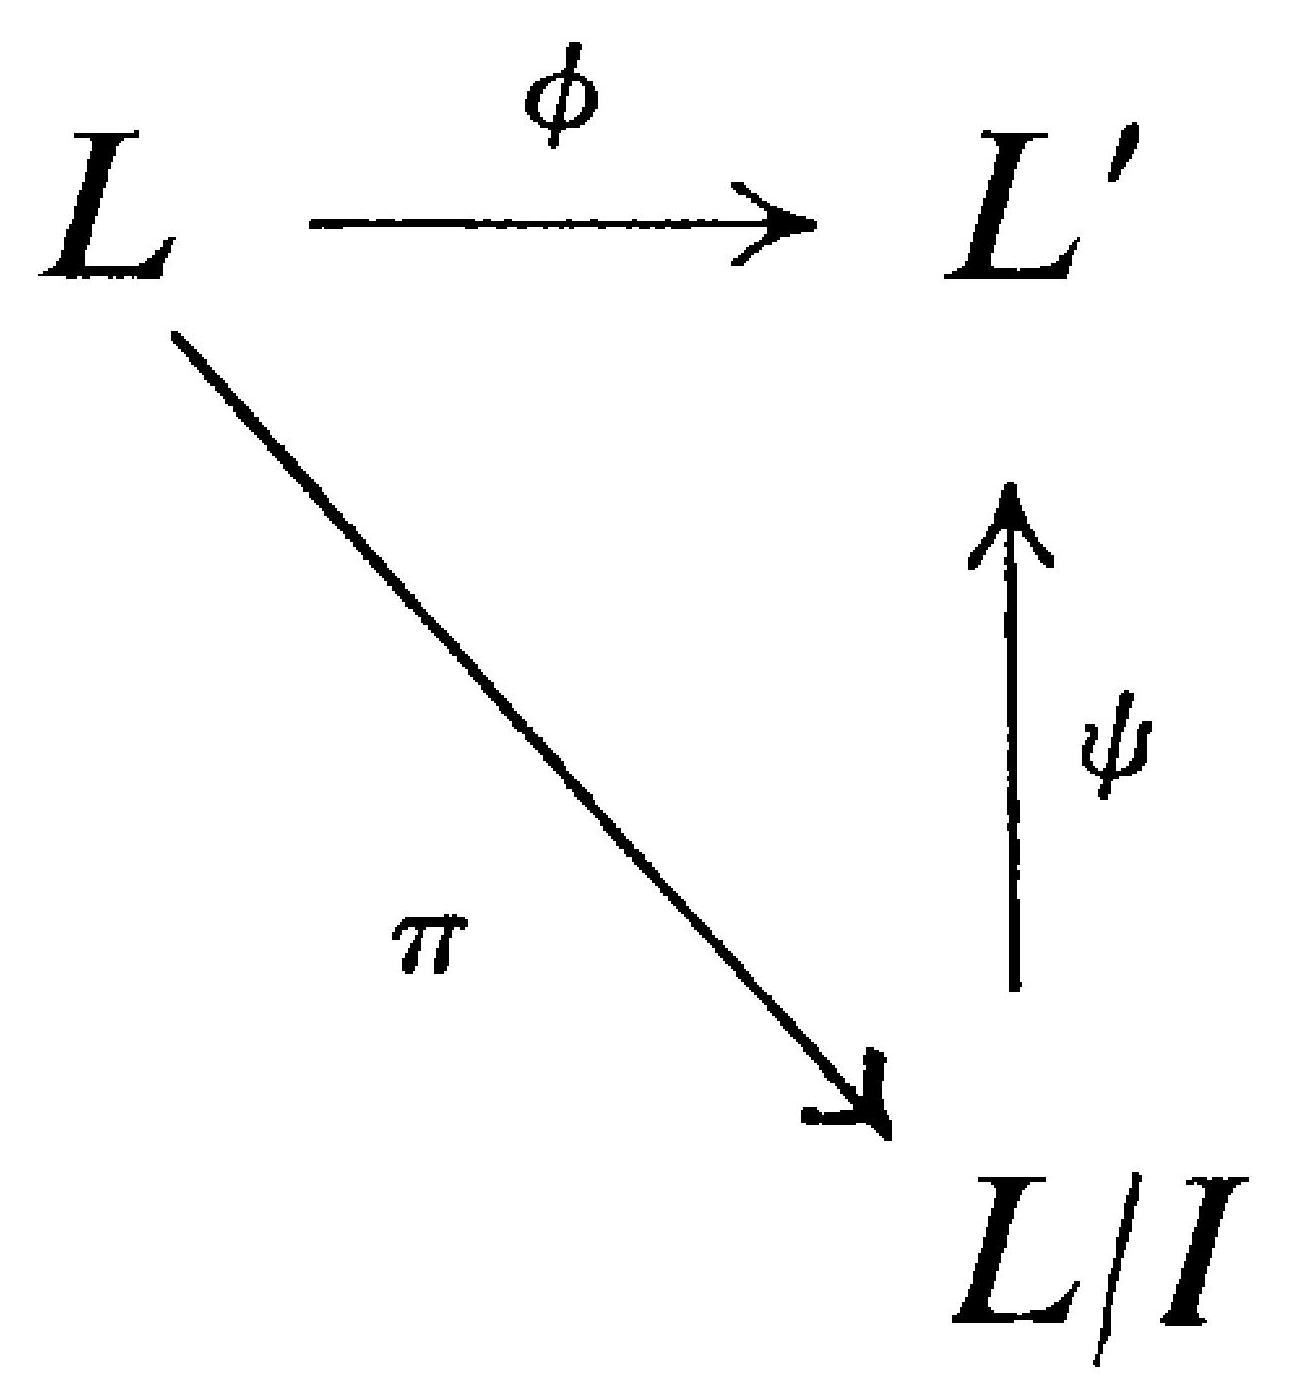
\includegraphics[max width=\textwidth, center]{2025_06_06_fac2836a92464059da43g-020}\\
(b) If $I$ and $J$ are ideals of $L$ such that $I \subset J$, then $J / I$ is an ideal of $L / I$ and $(L / I) /(J / I)$ is naturally isomorphic to $L / J$.\\
(c) If $I, J$ are ideals of $L$, there is a natural isomorphism between $(I+J) / J$ and $I /(I \cap J)$.

A representation of a Lie algebra $L$ is a homomorphism $\phi: L \rightarrow \mathfrak{g l}(V)$ ( $V=$ vector space over F ). Although we require $L$ to be finite dimensional, it is useful to allow $V$ to be of arbitrary dimension: $\mathfrak{g l}(V)$ makes sense in any case. However, for the time being the only important example to keep in mind is the adjoint representation ad: $L \rightarrow \mathfrak{g l}(L)$ introduced in (1.3), which sends $x$ to ad $x$, where ad $x(y)=[x y]$. (The image of ad is in Der $L \subset \mathfrak{g l}(L)$, but this does not concern us at the moment.) It is clear that ad is a linear transformation. To see that it preserves the bracket, we calculate:


\begin{align*}
\operatorname{ad} x, \operatorname{ad} y](z) & =\operatorname{ad} x \operatorname{ad} y(z)-\operatorname{ad} y \operatorname{ad} x(z) \\
& =\operatorname{ad} x([y z])-\operatorname{ad} y([x z]) \\
& =[x[y z]]-[y[x z]] \\
& =[x[y z]]+[[x z] y]  \tag{$L2$'}\\
& =[[x y] z]  \tag{L3}\\
& =\operatorname{ad}[x y](z)
\end{align*}


What is the kernel of ad? It consists of all $x \in L$ for which ad $x=0$, i.e., for which $[x y]=0$ (all $y \in L$ ). So Ker ad $=Z(L)$. This already has an interesting consequence: If $L$ is simple, then $Z(L)=0$, so that ad: $L \rightarrow \mathfrak{g l}(L)$ is a monomorphism. This means that any simple Lie algebra is isomorphic to a linear Lie algebra.

\subsection*{2.3. Automorphisms}
An automorphism of $L$ is an isomorphism of $L$ onto itself. Aut $L$ denotes the group of all such. Important examples occur when $L$ is a linear Lie algebra $\subset \mathfrak{g l}(V)$. If $g \in G L(V)$ is any invertible endomorphism of $V$, and if moreover $g L g^{-1}=L$, then it is immediate that the map $x \mapsto g x g^{-1}$ is an automorphism of $L$. For instance, if $L=\mathfrak{g l}(V)$ or even $\mathfrak{s l}(V)$, the second condition is automatic, so we obtain in this way a large collection of automorphisms. (Cf. Exercise 12.)

Now specialize to the case: char $\mathrm{F}=0$. Suppose $x \in L$ is an element for which ad $x$ is nilpotent, i.e., $(\operatorname{ad} x)^{k}=0$ for some $k>0$. Then the usual exponential power series for a linear transformation over $\mathbf{C}$ makes sense over F , because it has only finitely many terms: $\exp (\operatorname{ad} x)=1+\operatorname{ad} x+(\operatorname{ad} x)^{2} / 2$ ! $+(\operatorname{ad} x)^{3} / 3!+\ldots+(\operatorname{ad} x)^{k-1} /(k-1)!$. We claim that $\exp (\operatorname{ad} x) \in$ Aut $L$. More generally, this is true if ad $x$ is replaced by an arbitrary nilpotent derivation $\delta$ of L. For this, use the familiar Leibniz rule:

$$
\frac{\delta^{n}}{n!}(x y)=\sum_{i=0}^{n}(1 / i!)\left(\delta^{i} x\right)(1 /(n-i)!)\left(\delta^{n-i} y\right)
$$

Then calculate as follows: (say $\delta^{k}=0$ )

$$
\begin{aligned}
\exp \delta(x) \exp \delta(y) & =\left(\sum_{i=0}^{k-1}\left(\frac{\delta^{i} x}{i!}\right)\right)\left(\sum_{j=0}^{k-1}\left(\frac{\delta^{j} y}{j!}\right)\right) & & \\
& =\sum_{n=0}^{2 k-2}\left(\sum_{i=0}^{n}\left(\frac{\delta^{i} x}{i!}\right)\left(\frac{\delta^{n-i} y}{(n-i)!}\right)\right) & & \\
& =\sum_{n=0}^{2 k-2} \frac{\delta^{n}(x y)}{n!} & & (\text { Leibniz }) \\
& =\sum_{n=0}^{k-1} \frac{\delta^{n}(x y)}{n!} & & \left(\delta^{k}=0\right) \\
& =\exp \delta(x y) . & &
\end{aligned}
$$

The fact that $\exp \delta$ is invertible follows (in the usual way) by exhibiting the explicit inverse $1-\eta+\eta^{2}-\eta^{3}+\ldots \pm \eta^{k-1}, \exp \delta=1+\eta$.

An automorphism of the form $\exp (\operatorname{ad} x)$, ad $x$ nilpotent, is called inner; more generally, the subgroup of Aut $L$ generated by these is denoted Int $L$ and its elements called inner automorphisms. It is a normal subgroup: If $\phi \in$ Aut $L, x \in L$, then $\phi(\operatorname{ad} x) \phi^{-1}=\operatorname{ad} \phi(x)$, whence $\phi \exp (\operatorname{ad} x) \phi^{-1}=$ $\exp (\operatorname{ad} \phi(x))$.

For example, let $L=\mathfrak{s l}(2, \mathrm{~F})$, with standard basis ( $x, y, h$ ). Define $\sigma=\exp$ ad $x \cdot \exp$ ad $(-y) \cdot \exp$ ad $x$ (so $\sigma \in \operatorname{Int} L$ ). It is easy to compute the effect of $\sigma$ on the basis (Exercise 10): $\sigma(x)=-y, \sigma(y)=-x, \sigma(h)=-h$. In particular, $\sigma$ has order 2. Notice that $\exp x, \exp (-y)$ are well defined elements of $S L(2, \mathrm{~F})$, the group of $2 \times 2$ matrices of det 1 , conjugation by which leaves $L$ invariant (as noted at the start of this subsection), so the product $s=(\exp x)(\exp -y)(\exp x)$ induces an automorphism $z \mapsto s z s^{-1}$ of $L$. A quick calculation shows that $s=\left(\begin{array}{rr}0 & 1 \\ -1 & 0\end{array}\right)$ and that conjugating by $s$ has precisely the same effect on $L$ as applying $\sigma$.

The phenomenon just observed is not accidental: If $L \subset \mathfrak{g l}(V)$ is an arbitrary linear Lie algebra (char $\mathrm{F}=0$ ), and $x \in L$ is nilpotent, then we claim that


\begin{equation*}
(\exp x) y(\exp x)^{-1}=\exp \text { ad } x(y) \text { for all } y \in L . \tag{*}
\end{equation*}


To prove this, notice that ad $x=\lambda_{x}+\rho_{-x}$, where $\lambda_{x}, \rho_{x}$ denote left and right multiplication by $x$ in the ring End $V$ (these commute, of course, and are nilpotent). Then the usual rules of exponentiation show that exp ad $x=\exp \left(\lambda_{x}+\rho_{-x}\right)=\exp \lambda_{x} \cdot \exp \rho_{-x}=\lambda_{\exp x} \cdot \rho_{\exp (-x)}$, which implies (*).

\section*{Exercises}
\begin{enumerate}
  \item Prove that the set of all inner derivations ad $x, x \in L$, is an ideal of Der $L$.
  \item Show that $\mathfrak{s l}(n, \mathrm{~F})$ is precisely the derived algebra of $\mathrm{gl}(n, \mathrm{~F})$ (cf. Exercise 1.9).
  \item Prove that the center of $\mathfrak{g l}(n, \mathrm{~F})$ equals $\mathfrak{s}(n, \mathrm{~F})$ (the scalar matrices). Prove that $\mathfrak{s l}(n, \mathcal{F})$ has center 0 , unless char $\mathcal{F}$ divides $n$, in which case the center is $\mathfrak{s}(n, \mathrm{~F})$.
  \item Show that (up to isomorphism) there is a unique Lie algebra over $F$ of dimension 3 whose derived algebra has dimension 1 and lies in $Z(L)$.
  \item Suppose $\operatorname{dim} L=3, L=[L L]$. Prove that $L$ must be simple. [Observe first that any homomorphic image of $L$ also equals its derived algebra.] Recover the simplicity of $\mathfrak{s l}(2, \mathrm{~F})$, char $\mathrm{F} \neq 2$.
  \item Prove that $\mathfrak{s l}(3, F)$ is simple, unless char $F=3$ (cf. Exercise 3). [Use the standard basis $h_{1}, h_{2}, e_{i j}(i \neq j)$. If $I \neq 0$ is an ideal, then $I$ is the direct sum of eigenspaces for ad $h_{1}$ or ad $h_{2}$; compare the eigenvalues of ad $h_{1}$, ad $h_{2}$ acting on the $e_{1 j^{*}}$ ]
  \item Prove that $f(n, F)$ and $\delta(n, F)$ are self-normalizing subalgebras of $g l(n, F)$, whereas $n(n, F)$ has normalizer $t(n, F)$.
  \item Prove that in each classical linear Lie algebra (1.2), the set of diagonal matrices is a self-normalizing subalgebra, when char $F=0$.
  \item Prove Proposition 2.2.
  \item Let $\sigma$ be the automorphism of $\mathfrak{s l}(2, F)$ defined in (2.3). Verify that $\sigma(x)=-y, \sigma(y)=-x, \sigma(h)=-h$.
  \item If $L=\mathfrak{s l}(n, \mathrm{~F}), g \in G L(n, \mathrm{~F})$, prove that the map of $L$ to itself defined by $x \mapsto-g x^{t} g^{-1}\left(x^{t}=\right.$ transpose of $\left.x\right)$ belongs to Aut $L$. When $n=2$, $g=$ identity matrix, prove that this automorphism is inner.
  \item Let $L$ be an orthogonal Lie algebra (type $B_{\ell}$ or $D_{\ell}$ ). If $g$ is an orthogonal matrix, in the sense that $g$ is invertible and $g^{t} s g=s$, prove that $x \mapsto g x g^{-1}$ defines an automorphism of $L$.
\end{enumerate}

\section*{3. Solvable and nilpotent Lie algebras}
\subsection*{3.1. Solvability}
It is natural to study a Lie algebra $L$ via its ideals. In this section we exploit the formation of derived algebras. First, define a sequence of ideals of $L$ (the derived series) by $L^{(0)}=L, L^{(1)}=[L L], L^{(2)}=\left[L^{(1)} L^{(1)}\right], \ldots, L^{(i)}=$ $\left[L^{(i-1)} L^{(i-1)}\right]$. Call $L$ solvable if $L^{(n)}=0$ for some $n$. For example, abelian implies solvable, whereas simple algebras are definitely nonsolvable.

An example which turns out to be rather general is the algebra $\mathfrak{t}(n, \mathcal{F})$ of upper triangular matrices, which was introduced in (1.2). The obvious basis for $\mathrm{t}(n, \mathrm{~F})$ consists of the matrix units $e_{i j}$ for which $i \leq j$; the dimension is $1+2+\ldots+n=n(n+1) / 2$. To show that $L=\mathrm{t}(n, \mathrm{~F})$ is solvable we compute explicitly its derived series, using the formula for commutators in (1.2). In particular, we have $\left[e_{i i}, e_{i l}\right]=e_{i l}$ for $i<l$, which shows that $\mathfrak{n}(n, \mathfrak{F}) \subset[L L]$, where $\mathfrak{n}(n, \mathrm{~F})$ is the subalgebra of upper triangular nilpotent matrices. Since $\mathrm{t}(n, \mathrm{~F})=\mathfrak{d}(n, \mathrm{~F})+\mathfrak{n}(n, \mathrm{~F})$, and since $\mathfrak{d}(n, \mathrm{~F})$ is abelian, we conclude that $n(n, F)$ is equal to the derived algebra of $L$ (cf. Exercise 1.5). Working next inside the algebra $\mathfrak{n}(n, \mathrm{~F})$, we have a natural notion of "level" for $e_{i j}$, namely\\
$j-i$. In the formula for commutators, assume that $i<j, k<l$. Without losing any products we may also require $i \neq l$. Then $\left[e_{t j}, e_{k l}\right]=e_{t l}$ (if $j=k$ ) or 0 (otherwise). In particular, each $e_{i l}$ is commutator of two matrices whose levels add up to that of $e_{i l}$. We conclude that $L^{(2)}$ is spanned by those $e_{i j}$ of level $\geq 2, L^{(i)}$ by those of level $\geq 2^{i-1}$. Finally, it is clear that $L^{(i)}=0$ whenever $2^{i-1}>n-1$.

Next we assemble a few simple observations about solvability.\\
Proposition. Let $L$ be a Lie algebra.\\
(a) If $L$ is solvable, then so are all subalgebras and homomorphic images of $L$.\\
(b) If $I$ is a solvable ideal of $L$ such that $L / I$ is solvable, then $L$ itself is solvable.\\
(c) If $I, J$ are solvable ideals of $L$, then so is $I+J$.

Proof. (a) From the definition, if $K$ is a subalgebra of $L$, then $K^{(i)} \subset L^{(i)}$. Similarly, if $\phi: L \rightarrow M$ is an epimorphism, an easy induction on $i$ shows that $\phi\left(L^{(i)}\right)=M^{(i)}$.\\
(b) Say $(L / I)^{(n)}=0$. Applying part (a) to the canonical homomorphism $\pi: L \rightarrow L / I$, we get $\pi\left(L^{(n)}\right)=0$, or $L^{(n)} \subset I=$ Ker $\pi$. Now if $I^{(m)}=0$, the obvious fact that $\left(L^{(i)}\right)^{(j)}=L^{(i+j)}$ implies that $L^{(n+m)}=0$ (apply proof of part (a) to the situation $\left.L^{(n)} \subset I\right)$.\\
(c) One of the standard homomorphism theorems (Proposition 2.2 (c)) yields an isomorphism between $(I+J) / J$ and $I /(I \cap J)$. As a homomorphic image of $I$, the right side is solvable, so $(I+J) / J$ is solvable. Then so is $I+J$, by part (b) applied to the pair $I+J, J . \quad \square$

As a first application, let $L$ be an arbitrary Lie algebra and let $S$ be a maximal solvable ideal (i.e., one included in no larger solvable ideal). If $I$ is any other solvable ideal of $L$, then part (c) of the Proposition forces $S+I=S$ (by maximality), or $I \subset S$. This proves the existence of a unique maximal solvable ideal, called the radical of $L$ and denoted $\operatorname{Rad} L$. In case $\operatorname{Rad} L=0, L$ is called semisimple. For example, a simple algebra is semisimple: $L$ has no ideals except itself and 0 , and $L$ is nonsolvable. Also, $L=0$ is semisimple. Notice that for arbitrary $L, L / \operatorname{Rad} L$ is semisimple (use part (b) of the proposition). The study of semisimple Lie algebras (char $F=0$ ) will occupy most of this book. (But certain solvable subalgebras will also be needed along the way.)

\subsection*{3.2. Nilpotency}
The definition of solvability imitates the corresponding notion in group theory, which goes back to Abel and Galois. By contrast, the notion of nilpotent group is more recent, and is modeled on the corresponding notion for Lie algebras. Define a sequence of ideals of $L$ (the descending central series, also called the lower central series) by $L^{0}=L, L^{1}=[L L]\left(=L^{(1)}\right)$, $L^{2}=\left[L L^{1}\right], \ldots, L^{i}=\left[L L^{i-1}\right] . L$ is called nilpotent if $L^{n}=0$ for some $n$. For example, any abelian algebra is nilpotent. Clearly, $L^{(i)} \subset L^{i}$ for all $i$, so\\
nilpotent algebras are solvable. The converse is false, however. Consider again $L=\mathrm{t}(n, \mathrm{~F})$. Our discussion in (3.1) showed that $L^{(1)}=L^{1}$ is $\mathrm{n}(n, \mathrm{~F})$, and also that $L^{2}=\left[L L^{1}\right]=L^{1}$, so $L^{i}=L^{1}$ for all $i \geq 1$. On the other hand, it is easy to see that $M=\mathfrak{n}(n, \mathfrak{F})$ is nilpotent: $M^{1}$ is spanned by those $e_{i j}$ of level $\geq 2, M^{2}$ by those of level $\geq 3, \ldots, M^{i}$ by those of level $\geq i+1$.

\section*{Proposition. Let L be a Lie algebra.}
(a) If $L$ is nilpotent, then so are all subalgebras and homomorphic images of $L$.\\
(b) If $L / Z(L)$ is nilpotent, then so is $L$.\\
(c) If $L$ is nilpotent and nonzero, then $Z(L) \neq 0$.

Proof. (a) Imitate the proof of Proposition 3.1 (a).\\
(b) Say $L^{n} \subset Z(L)$, then $L^{n+1}=\left[L L^{n}\right] \subset[L Z(L)]=0$.\\
(c) The last nonzero term of the descending central series is central.

The condition for $L$ to be nilpotent can be rephrased as follows: For some $n$ (depending only on $L$ ), ad $x_{1}$ ad $x_{2} \ldots$ ad $x_{n}(y)=0$ for all $x_{i}, y \in L$. In particular, $(\operatorname{ad} x)^{n}=0$ for all $x \in L$. Now if $L$ is any Lie algebra, and $x \in L$, we call $x$ ad-nilpotent if ad $x$ is a nilpotent endomorphism. Using this language, our conclusion can be stated: If $L$ is nilpotent, then all elements of $L$ are adnilpotent. It is a pleasant surprise to find that the converse is also true.

Theorem (Engel). If all elements of $L$ are ad-nilpotent, then $L$ is nilpotent.\\
The proof will be given in the next subsection. Using Engel's Theorem, it is easy to prove that $\mathfrak{n}(n, \mathfrak{F})$ is nilpotent, without actually calculating the descending central series. We need only apply the following simple lemma.

Lemma. Let $x \in \mathfrak{g l}(V)$ be a nilpotent endomorphism. Then ad $x$ is also nilpotent.

Proof. As in (2.3), we may associate to $x$ two endomorphisms of End $V$, left and right translation: $\lambda_{x}(y)=x y, \rho_{x}(y)=y x$, which are nilpotent because $x$ is. Moreover $\lambda_{x}$ and $\rho_{x}$ obviously commute. In any ring (here End (End $V$ )) the sum or difference of two commuting nilpotents is again nilpotent (why?), so ad $x=\lambda_{x}-\rho_{x}$ is nilpotent.

A word of warning: It is easy for a matrix to be ad-nilpotent in $\mathfrak{g l}(n, \mathcal{F})$ without being nilpotent. (The identity matrix is an example.) The reader should keep in mind two contrasting types of nilpotent linear Lie algebras: $\mathfrak{d}(n, F)$ and $\mathfrak{n}(n, F)$.

\subsection*{3.3. Proof of Engel's Theorem}
Engel's Theorem (3.2) will be deduced from the following result, which is of interest in its own right. Recall that a single nilpotent linear transformation always has at least one eigenvector, corresponding to its unique eigenvalue 0 . This is just the case $\operatorname{dim} L=1$ of the following theorem.

Theorem. Let $L$ be a subalgebra of $\mathfrak{g l}(V), V$ finite dimensional. If $L$ consists of nilpotent endomorphisms and $V \neq 0$, then there exists nonzero $v \in V$ for which $L . v=0$.

Proof. Use induction on $\operatorname{dim} L$, the case $\operatorname{dim} L=0$ (or $\operatorname{dim} L=1$ ) being obvious. Suppose $K \neq L$ is any subalgebra of $L$. According to Lemma 3.2, $K$ acts (via ad) as a Lie algebra of nilpotent linear transformations on the vector space $L$, hence also on the vector space $L / K$. Because $\operatorname{dim} K<$ $\operatorname{dim} L$, the induction hypothesis guarantees existence of a vector $x+K \neq K$ in $L / K$ killed by the image of $K$ in $\mathfrak{g l}(L / K)$. This just means that $[y x] \in K$ for all $y \in K$, whereas $x \notin K$. In other words, $K$ is properly included in $N_{L}(K)$ (the normalizer of $K$ in $L$, see (2.1)).

Now take $K$ to be a maximal proper subalgebra of $L$. The preceding argument forces $N_{L}(K)=L$, i.e., $K$ is an ideal of $L$. If dim $L / K$ were greater than one, then the inverse image in $L$ of a one dimensional subalgebra of $L / K$ (which always exists) would be a proper subalgebra properly containing $K$, which is absurd; therefore, $K$ has codimension one. This allows us to write $L=K+\mathrm{F} z$ for any $z \in L-K$.

By induction, $W=\{v \in V \mid K \cdot v=0\}$ is nonzero. Since $K$ is an ideal, $W$ is stable under $L: x \in L, y \in K, w \in W$ imply $y x \cdot w=x y \cdot w-[x, y] \cdot w=0$. Choose $z \in L-K$ as above, so the nilpotent endomorphism $z$ (acting now on the subspace $W$ ) has an eigenvector, i.e., there exists nonzero $v \in W$ for which $z \cdot v=0$. Finally, L.v $=0$, as desired.

Proof of Engel's Theorem. We are given a Lie algebra $L$ all of whose elements are ad-nilpotent; therefore, the algebra ad $L \subset \mathfrak{g l}(L)$ satisfies the hypothesis of Theorem 3.3. (We can assume $L \neq 0$.) Conclusion: There exists $x \neq 0$ in $L$ for which $[L x]=0$, i.e., $Z(L) \neq 0$. Now $L / Z(L)$ evidently consists of ad-nilpotent elements and has smaller dimension than $L$. Using induction on $\operatorname{dim} L$, we find that $L / Z(L)$ is nilpotent. Part (b) of Proposition 3.2 then implies that $L$ itself is nilpotent.

There is a useful corollary (actually, an equivalent version) of Theorem 3.3, which shows how "typical" $\mathrm{n}(n, \mathrm{~F})$ is. First a definition: If $V$ is a finite dimensional vector space (say $\operatorname{dim} V=n$ ), a flag in $V$ is a chain of subspaces $0=V_{0} \subset V_{1} \subset \ldots \subset V_{n}=V, \operatorname{dim} V_{i}=i$. If $x \in \operatorname{End} V$, we say $x$ stabilizes (or leaves invariant) this flag provided $x . V_{i} \subset V_{i}$ for all $i$.

Corollary. Under the hypotheses of the theorem there exists a flag $\left(V_{i}\right)$ in $V$ stable under $L$, with $x . V_{i} \subset V_{i-1}$ for all $i$. In other words, there exists a basis of $V$ relative to which the matrices of $L$ are all in $\mathfrak{n}(n, F)$.

Proof. Begin with any nonzero $v \in V$ killed by $L$, the existence of which is assured by the theorem. Set $V_{1}=\mathrm{F} v$. Let $W=V / V_{1}$, and observe that the induced action of $L$ on $W$ is also by nilpotent endomorphisms. By induction on $\operatorname{dim} V, W$ has a flag stabilized by $L$, whose inverse image in $V$ does the trick.

To conclude this section, we mention a typical application of Theorem 3.3, which will be needed later on.

Lemma. Let $L$ be nilpotent, $K$ an ideal of $L$. Then if $K \neq 0, K \cap Z(L) \neq 0$. (In particular, $Z(L) \neq 0$; cf. Proposition 3.2(c).)

Proof. $L$ acts on $K$ via the adjoint representation, so Theorem 3.3 yields nonzero $x \in K$ killed by $L$, i.e., $[L x]=0$, so $x \in K \cap Z(L)$.

\section*{Exercises}
\begin{enumerate}
  \item Let $I$ be an ideal of $L$. Then each member of the derived series or descending central series of $I$ is also an ideal of $L$.
  \item Prove that $L$ is solvable if and only if there exists a chain of subalgebras $L=L_{0} \supset L_{1} \supset L_{2} \supset \ldots \supset L_{k}=0$ such that $L_{i+1}$ is an ideal of $L_{i}$ and such that each quotient $L_{i} / L_{i+1}$ is abelian.
  \item Let char $\mathrm{F}=2$. Prove that $\mathfrak{s l}(2, \mathrm{~F})$ is nilpotent.
  \item Prove that $L$ is solvable (resp. nilpotent) if and only if ad $L$ is solvable (resp. nilpotent).
  \item Prove that the nonabelian two dimensional algebra constructed in (1.4) is solvable but not nilpotent. Do the same for the algebra in Exercise 1.2.
  \item Prove that the sum of two nilpotent ideals of a Lie algebra $L$ is again a nilpotent ideal. Therefore, $L$ possesses a unique maximal nilpotent ideal. Determine this ideal for each algebra in Exercise 5.
  \item Let $L$ be nilpotent, $K$ a proper subalgebra of $L$. Prove that $N_{L}(K)$ includes $K$ properly.
  \item Let $L$ be nilpotent. Prove that $L$ has an ideal of codimension 1 .
  \item Prove that every nilpotent Lie algebra $L$ has an outer derivation (see (1.3)), as follows: Write $L=K+\mathrm{F} x$ for some ideal $K$ of codimension one (Exercise 8). Then $C_{L}(K) \neq 0$ (why?). Choose $n$ so that $C_{L}(K) \subset L^{n}$, $C_{L}(K) \notin L^{n+1}$, and let $z \in C_{L}(K)-L^{n+1}$. Then the linear map $\delta$ sending $K$ to $0, x$ to $z$, is an outer derivation.
  \item Let $L$ be a Lie algebra, $K$ an ideal of $L$ such that $L / K$ is nilpotent and such that ad $\left.x\right|_{K}$ is nilpotent for all $x \in L$. Prove that $L$ is nilpotent.
\end{enumerate}

\section*{Chapter II}
\section*{Semisimple Lie Algebras}
In Chapter I we looked at Lie algebras over an arbitrary field F. Apart from introducing the basic notions and examples, we were able to prove only one substantial theorem (Engel's Theorem). Virtually all of the remaining theory to be developed in this book will require the assumption that $F$ have characteristic 0. (Some of the exercises will indicate how counterexamples arise in prime characteristic.) Moreover, in order to have available the eigenvalues of ad $x$ for arbitrary $x$ (not just for ad $x$ nilpotent), we shall assume that $F$ is algebraically closed, except where otherwise specified. It is possible to work with a slightly less restrictive assumption on F (cf. Jacobson [1], p. 107), but we shall not do so here.

\section*{4. Theorems of Lie and Cartan}
\subsection*{4.1. Lie's Theorem}
The essence of Engel's Theorem for nilpotent Lie algebras is the existence of a common eigenvector for a Lie algebra consisting of nilpotent endomorphisms (Theorem 3.3). The next theorem is similar in nature, but requires algebraic closure, in order to assure that $F$ will contain all required eigenvalues. It turns out to be necessary also to have char $\mathrm{F}=0$ (Exercise 3).

Theorem. Let $L$ be a solvable subalgebra of $\mathfrak{g l}(V), V$ finite dimensional. If $V \neq 0$, then $V$ contains a common eigenvector for all the endomorphisms in $L$.

Proof. Use induction on $\operatorname{dim} L$, the case $\operatorname{dim} L=0$ being trivial. We attempt to imitate the proof of Theorem 3.3 (which the reader should review at this point). The idea is (1) to locate an ideal $K$ of codimension one, (2) to show by induction that common eigenvectors exist for $K$, (3) to verify that $L$ stabilizes a space consisting of such eigenvectors, and (4) to find in that space an eigenvector for a single $z \in L$ satisfying $L=K+\mathrm{F} z$.

Step (1) is easy. Since $L$ is solvable, of positive dimension, $L$ properly includes [ $L L$ ]. $L /[L L]$ being abelian, any subspace is automatically an ideal. Take a subspace of codimension one, then its inverse image $K$ is an ideal of codimension one in $L$ (including [ $L L$ ]).

For step (2), use induction to find a common eigenvector $v \in V$ for $K$ ( $K$ is of course solvable; if $K=0$, then $L$ is abelian of dimension 1 and an eigenvector for a basis vector of $L$ finishes the proof.) This means that for $x \in K$\\
$x . v=\lambda(x) v, \lambda: K \rightarrow \mathrm{~F}$ some linear function. Fix this $\lambda$, and denote by $W$ the subspace

$$
\{w \in V \mid x . w=\lambda(x) w, \text { for all } x \in K\} ; \text { so } W \neq 0 .
$$

Step (3) consists in showing that $L$ leaves $W$ invariant. Assuming for the moment that this is done, proceed to step (4): Write $L=K+\mathrm{F} z$, and use the fact that F is algebraically closed to find an eigenvector $v_{0} \in W$ of $z$ (for some eigenvalue of $z$ ). Then $v_{0}$ is obviously a common eigenvector for $L$ (and $\lambda$ can be extended to a linear function on $L$ such that $x \cdot v_{0}=\lambda(x) v_{0}$, $x \in L)$.

It remains to show that $L$ stabilizes $W$. Let $w \in W, x \in L$. To test whether or not $x . w$ lies in $W$, we must take arbitrary $y \in K$ and examine $y x . w=$ $x y \cdot w-[x, y] \cdot w=\lambda(y) x \cdot w-\lambda([x, y]) w$. Thus we have to prove that $\lambda([x, y])=0$. For this, fix $w \in W, x \in L$. Let $n>0$ be the smallest integer for which $w$, $x . w, \ldots, x^{n} . w$ are linearly dependent. Let $W_{i}$ be the subspace of $V$ spanned by $w, x . w, \ldots, x^{i-1} . w$ (set $W_{0}=0$ ), so $\operatorname{dim} W_{n}=n, W_{n}=W_{n+i}(i \geq 0)$ and $x$ maps $W_{n}$ into $W_{n}$. It is easy to check that each $y \in K$ leaves each $W_{i}$ invariant. Relative to the basis $w, x . w, \ldots, x^{n-1} . w$ of $W_{n}$, we claim that $y \in K$ is represented by an upper triangular matrix whose diagonal entries equal $\lambda(y)$. This follows immediately from the congruence:


\begin{equation*}
y x^{i} \cdot w \equiv \lambda(y) x^{i} \cdot w\left(\bmod W_{i}\right), \tag{*}
\end{equation*}


which we prove by induction on $i$, the case $i=0$ being obvious. Write $y x^{i} \cdot w=y x x^{i-1} \cdot w=x y x^{i-1} \cdot w-[x, y] x^{i-1} \cdot w$. By induction, $y x^{i-1} \cdot w=$ $\lambda(y) x^{i-1} \cdot w+w^{\prime}\left(w^{\prime} \in W_{i-1}\right)$; since $x$ maps $W_{i-1}$ into $W_{i}$ (by construction), $\left(^{*}\right)$ therefore holds for all $i$.

According to our description of the way in which $y \in K$ acts on $W_{n}$, $\operatorname{Tr}_{W_{n}}(y)=n \lambda(y)$. In particular, this is true for elements of $K$ of the special form $[x, y]$ ( $x$ as above, $y$ in $K$ ). But $x, y$ both stabilize $W_{n}$, so $[x, y]$ acts on $W_{n}$ as the commutator of two endomorphisms of $W_{n}$; its trace is therefore 0 . We conclude that $n \lambda([x, y])=0$. Since char $\mathrm{F}=0$, this forces $\lambda([x, y])=0$, as required.

Corollary A (Lie's Theorem). Let $L$ be a solvable subalgebra of $\mathfrak{g l}(V)$, $\operatorname{dim} V=n<\infty$. Then $L$ stabilizes some flag in $V$ (in other words, the matrices of $L$ relative to a suitable basis of $V$ are upper triangular).

Proof. Use the theorem, along with induction on $\operatorname{dim} V$.\\
More generally, let $L$ be any solvable Lie algebra, $\phi: L \rightarrow \mathfrak{g l}(V)$ a finite dimensional representation of $L$. Then $\phi(L)$ is solvable, by Proposition 3.1(a), hence stabilizes a flag (Corollary A). For example, if $\phi$ is the adjoint representation, a flag of subspaces stable under $L$ is just a chain of ideals of $L$, each of codimension one in the next. This proves:

Corollary B. Let $L$ be solvable. Then there exists a chain of ideals of $L$, $0=L_{0} \subset L_{1} \subset \ldots \subset L_{n}=L$, such that $\operatorname{dim} L_{i}=i$.

Corollary C. Let $L$ be solvable. Then $x \in[L L]$ implies that ad $d_{L} x$ is nilpotent. In particular, $[L L]$ is nilpotent.

Proof. Find a flag of ideals as in Corollary B. Relative to a basis ( $x_{1}, \ldots$, $x_{n}$ ) of $L$ for which ( $x_{1}, \ldots, x_{i}$ ) spans $L_{i}$, the matrices of ad $L$ lie in $\mathrm{t}(n, \mathrm{~F})$. Therefore the matrices of $[\operatorname{ad} L, \operatorname{ad} L]=\operatorname{ad}_{L}[L L]$ lie in $\mathfrak{n}(n, \mathcal{F})$, the derived algebra of $\mathrm{t}(n, \mathrm{~F})$. It follows that $\operatorname{ad}_{L} x$ is nilpotent for $x \in[L L]$; a fortiori $\operatorname{ad}_{[L L]} x$ is nilpotent, so $[L L]$ is nilpotent by Engel's Theorem.

\subsection*{4.2. Jordan-Chevalley decomposition}
In this subsection only, char F may be arbitrary. We digress in order to introduce a very useful tool for the study of linear transformations. The reader may recall that the Jordan canonical form for a single endomorphism $x$ over an algebraically closed field amounts to an expression of $x$ in matrix form as a sum of blocks

$$
\left[\begin{array}{cccccc}
a & 1 & & & & 0 \\
& a & 1 & & & \\
& & \cdot & \cdot & & \\
& & & \cdot & \cdot & \\
& & & & \cdot & 1 \\
0 & & & & & a
\end{array}\right]
$$

Since $\operatorname{diag}(a, \ldots, a)$ commutes with the nilpotent matrix having one's just above the diagonal and zeros elsewhere, $x$ is the sum of a diagonal and a nilpotent matrix which commute. We can make this decomposition more precise, as follows.

Call $x \in$ End $V$ ( $V$ finite dimensional) semisimple if the roots of its minimal polynomial over $F$ are all distinct. Equivalently ( $F$ being algebraically closed), $x$ is semisimple if and only if $x$ is diagonalizable. We remark that two commuting semisimple endomorphisms can be simultaneously diagonalized; therefore, their sum or difference is again semisimple (Exercise 2). Also, if $x$ is semisimple and maps a subspace $W$ of $V$ into itself, then obviously the restriction of $x$ to $W$ is semisimple.

Proposition. Let $V$ be a finite dimensional vector space over $\mathrm{F}, x \in$ End $V$.\\
(a) There exist unique $x_{s}, x_{n} \in$ End $V$ satisfying the conditions: $x=x_{s}+x_{n}$, $x_{s}$ is semisimple, $x_{n}$ is nilpotent, $x_{s}$ and $x_{n}$ commute.\\
(b) There exist polynomials $p(T), q(T)$ in one indeterminate, without constant term, such that $x_{s}=p(x), x_{n}=q(x)$. In particular, $x_{s}$ and $x_{n}$ commute with any endomorphism commuting with $x$.\\
(c) If $A \subset B \subset V$ are subspaces, and $x$ maps $B$ into $A$, then $x_{s}$ and $x_{n}$ also map $B$ into $A$.

The decomposition $x=x_{s}+x_{n}$ is called the (additive) Jordan-Chevalley decomposition of $x$, or just the Jordan decomposition; $x_{s}, x_{n}$ are called (respectively) the semisimple part and the nilpotent part of $x$.

Proof. Let $a_{1}, \ldots, a_{k}$ (with multiplicities $m_{1}, \ldots, m_{k}$ ) be the distinct eigenvalues of $x$, so the characteristic polynomial is $\Pi\left(T-a_{i}\right)^{m_{i}}$. If $V_{i}=\operatorname{Ker}$ $\left(x-a_{i} \cdot 1\right)^{m_{i}}$, then $V$ is the direct sum of the subspaces $V_{1}, \ldots, V_{k}$, each stable\\
under $x$. On $V_{i}, x$ clearly has characteristic polynomial $\left(T-a_{i}\right)^{m_{i}}$. Now apply the Chinese Remainder Theorem (for the ring $\mathrm{F}[T]$ ) to locate a polynomial $p(T)$ satisfying the congruences, with pairwise relatively prime moduli: $p(T) \equiv a_{i}\left(\bmod \left(T-a_{i}\right)^{m_{i}}\right), p(T) \equiv 0(\bmod T$.) (Notice that the last congruence is superfluous if 0 is an eigenvalue of $x$, while otherwise $T$ is relatively prime to the other moduli.) Set $q(T)=T-p(T)$. Evidently each of $p(T), q(T)$ has zero constant term, since $p(T) \equiv 0(\bmod T)$.

Set $x_{s}=p(x), x_{n}=q(x)$. Since they are polynomials in $x, x_{s}$ and $x_{n}$ commute with each other, as well as with all endomorphisms which commute with $x$. They also stabilize all subspaces of $V$ stabilized by $x$, in particular the $V_{i}$. The congruence $p(T) \equiv a_{i}\left(\bmod \left(T-a_{i}\right)^{m_{i}}\right)$ shows that the restriction of $x_{s}-a_{i} \cdot 1$ to $V_{i}$ is zero for all $i$, hence that $x_{s}$ acts diagonally on $V_{i}$ with single eigenvalue $a_{i}$. By definition, $x_{n}=x-x_{s}$, which makes it clear that $x_{n}$ is nilpotent. Because $p(T), q(T)$ have no constant term, (c) is also obvious at this point.

It remains only to prove the uniqueness assertion in (a). Let $x=s+n$ be another such decomposition, so we have $x_{s}-s=n-x_{n}$. Because of (b), all endomorphisms in sight commute. Sums of commuting semisimple (resp. nilpotent) endomorphisms are again semisimple (resp. nilpotent), whereas only 0 can be both semisimple and nilpotent. This forces $s=x_{s}, n=x_{n} . \quad \square$

To indicate why the Jordan decomposition will be a valuable tool, we look at a special case. Consider the adjoint representation of the Lie algebra $\mathfrak{g l}(V), V$ finite dimensional. If $x \in \mathfrak{g l}(V)$ is nilpotent, then so is ad $x$ (Lemma 3.2). Similarly, if $x$ is semisimple, then so is ad $x$. We verify this as follows. Choose a basis $\left(v_{1}, \ldots, v_{n}\right)$ of $V$ relative to which $x$ has matrix diag $\left(a_{1}, \ldots\right.$, $\left.a_{n}\right)$. Let $\left\{e_{i j}\right\}$ be the standard basis of $g \mathfrak{l}(V)(1.2)$ relative to $\left(v_{1}, \ldots, v_{n}\right)$ : $e_{i j}\left(v_{k}\right)=\delta_{j k} v_{i}$. Then a quick calculation (see formula (*) in (1.2)) shows that ad $x\left(e_{i j}\right)=\left(a_{i}-a_{j}\right) e_{i j}$. So ad $x$ has diagonal matrix, relative to the chosen basis of $\mathrm{gl}(V)$.

Lemma A. Let $x \in$ End $V(\operatorname{dim} V<\infty), x=x_{s}+x_{n}$ its Jordan decomposition. Then ad $x=$ ad $x_{s}+$ ad $x_{n}$ is the Jordan decomposition of ad $x$ (in End (End V)).

Proof. We have seen that ad $x_{s}$, ad $x_{n}$ are respectively semisimple, nilpotent; they commute, since $\left[\operatorname{ad} x_{s}\right.$, ad $\left.x_{n}\right]=\operatorname{ad}\left[x_{s}, x_{n}\right]=0$. Then part (a) of the proposition applies.

A further useful fact is the following.\\
Lemma B. Let $\mathfrak{A}$ be a finite dimensional F-algebra. Then Der $\mathfrak{A}$ contains the semisimple and nilpotent parts (in End $\mathfrak{A}$ ) of all its elements.

Proof. If $\delta \in \operatorname{Der} \mathfrak{A}$, let $\sigma, \nu \in \operatorname{End} \mathfrak{A}$ be its semisimple and nilpotent parts, respectively. It will be enough to show that $\sigma \in \operatorname{Der} \mathfrak{A}$. If $a \in \mathrm{~F}$, set $\mathfrak{A}_{a}=\left\{x \in \mathfrak{A} \mid(\delta-a .1)^{k} x=0\right.$ for some $k$ (depending on $\left.\left.x\right)\right\}$. Then $\mathfrak{A}$ is the direct sum of those $\mathfrak{A}_{a}$ for which $a$ is an eigenvalue of $\delta$ (or $\sigma$ ), and $\sigma$ acts on $\mathfrak{A}_{a}$ as scalar multiplication by $a$. We can verify, for arbitrary $a, b \in \mathrm{~F}$, that $\mathfrak{A}_{a} \mathfrak{A}_{b} \subset \mathfrak{A}_{a+b}$, by means of the general formula: $\left(^{*}\right)(\delta-(a+b) .1)^{n}(x y)$\\
$=\sum_{i=0}^{n}\binom{n}{i}\left((\delta-a .1)^{n-i} x\right) \cdot\left((\delta-b .1)^{i} y\right)$, for $x, y \in \mathfrak{A}$. (This formula is easily checked by induction on $n$.) Now if $x \in \mathfrak{A}_{a}, y \in \mathfrak{A}_{b}$, then $\sigma(x y)=(a+b) x y$, because $x y \in \mathfrak{A}_{a+b}$ (possibly equal to 0 ); on the other hand, $(\sigma x) y+x(\sigma y)=$ $(a+b) x y$. By directness of the sum $\mathfrak{A}=\coprod \mathfrak{A}_{a}$, it follows that $\sigma$ is a derivation, as required.

\subsection*{4.3. Cartan's Criterion}
We are now ready to obtain a powerful criterion for solvability of a Lie algebra $L$, based on the traces of certain endomorphisms of $L$. It is obvious that $L$ will be solvable if $[L L]$ is nilpotent (this is the converse of Corollary 4.1C). In turn, Engel's Theorem says that [ $L L$ ] will be nilpotent if (and only if) each $\operatorname{ad}_{[L L]} x, x \in[L L]$, is nilpotent. We begin, therefore, with a "trace" criterion for nilpotence of an endomorphism.

Lemma. Let $A \subset B$ be two subspaces of $\mathfrak{g l}(V)$, dim $V<\infty$. Set $M=$ $\{x \in \mathfrak{g l}(V) \mid[x, B] \subset A\}$. Suppose $x \in M$ satisfies $\operatorname{Tr}(x y)=0$ for all $y \in M$. Then $x$ is nilpotent.

Proof. Let $x=s+n\left(s=x_{s}, n=x_{n}\right)$ be the Jordan decomposition of $x$. Fix a basis $v_{1}, \ldots, v_{m}$ of $V$ relative to which $s$ has matrix $\operatorname{diag}\left(a_{1}, \ldots, a_{m}\right)$. Let $E$ be the vector subspace of F (over the prime field $\mathbf{Q}$ ) spanned by the eigenvalues $a_{1}, \ldots, a_{m}$. We have to show that $s=0$, or equivalently, that $E=0$. Since $E$ has finite dimension over $\mathbf{Q}$ (by construction), it will suffice to show that the dual space $E^{*}$ is 0 , i.e., that any linear function $f: E \rightarrow \mathbf{Q}$ is zero.

Given $f$, let $y$ be that element of $\mathrm{gl}(V)$ whose matrix relative to our given basis is diag $\left(f\left(a_{1}\right), \ldots, f\left(a_{m}\right)\right)$. If $\left\{e_{i j}\right\}$ is the corresponding basis of $\mathfrak{g l}(V)$, we saw in (4.2) that: ad $s\left(e_{i j}\right)=\left(a_{i}-a_{j}\right) e_{i j}$, ad $y\left(e_{i j}\right)=\left(f\left(a_{i}\right)-f\left(a_{j}\right)\right) e_{i j}$. Now let $r(T) \in \mathrm{F}[T]$ be a polynomial without constant term satisfying $r\left(a_{i}-a_{j}\right)=$ $f\left(a_{i}\right)-f\left(a_{j}\right)$ for all pairs $i, j$. The existence of such $r(T)$ follows from Lagrange interpolation; there is no ambiguity in the assigned values, since $a_{i}-a_{j}=$ $a_{k}-a_{l}$ implies (by linearity of $f$ ) that $f\left(a_{i}\right)-f\left(a_{j}\right)=f\left(a_{k}\right)-f\left(a_{l}\right)$. Evidently $\operatorname{ad} y=r(\operatorname{ad} s)$.

Now ad $s$ is the semisimple part of ad $x$, by Lemma A of (4.2), so it can be written as a polynomial in ad $x$ without constant term (Proposition 4.2). Therefore, ad $y$ is also a polynomial in ad $x$ without constant term. By hypothesis, ad $x$ maps $B$ into $A$, so we also have ad $y(B) \subset A$, i.e., $y \in M$. Using the hypothesis of the lemma, $\operatorname{Tr}(x y)=0$, we get $\Sigma a_{i} f\left(a_{i}\right)=0$. The left side is a $\mathbf{Q}$-linear combination of elements of $E$; applying $f$, we obtain $\Sigma f\left(a_{i}\right)^{2}=0$. But the numbers $f\left(a_{i}\right)$ are rational, so this forces all of them to be 0 . Finally, $f$ must be identically 0 , because the $a_{i}$ span $E$.

Before stating our solvability criterion, we record a useful identity: If $x, y, z$ are endomorphisms of a finite dimensional vector space, then (*) $\operatorname{Tr}([x, y] z)=\operatorname{Tr}(x[y, z])$. To verify this, write $[x, y] z=x y z-y x z, x[y, z]$ $=x y z-x z y$, and use the fact that $\operatorname{Tr}(y(x z))=\operatorname{Tr}((x z) y)$.

Theorem (Cartan's Criterion). Let $L$ be a subalgebra of $\mathfrak{g l}(V), V$ finite dimensional. Suppose that $\operatorname{Tr}(x y)=0$ for all $x \in[L L], y \in L$. Then $L$ is solvable.

Proof. As remarked at the beginning of (4.3), it will suffice to prove that $[L L]$ is nilpotent, or just that all $x$ in $[L L]$ are nilpotent endomorphisms (Lemma 3.2 and Engel's Theorem). For this we apply the above lemma to the situation: $V$ as given, $A=[L L], B=L$, so $M=\{x \in \mathfrak{g l}(V) \mid[x, L] \subset$ $[L L]\}$. Obviously $L \subset M$. Our hypothesis is that $\operatorname{Tr}(x y)=0$ for $x \in[L L]$, $y \in L$, whereas to conclude from the lemma that each $x \in[L L]$ is nilpotent we need the stronger statement: $\operatorname{Tr}(x y)=0$ for $x \in[L L], y \in M$.

Now if $[x, y]$ is a typical generator of $[L L]$, and if $z \in M$, then identity (*) above shows that $\operatorname{Tr}([x, y] z)=\operatorname{Tr}(x[y, z])=\operatorname{Tr}([y, z] x)$. By definition of $M$, $[y, z] \in[L L]$, so the right side is 0 by hypothesis.

Corollary. Let $L$ be a Lie algebra such that $\operatorname{Tr}($ ad $x$ ad $y)=0$ for all $x \in[L L], y \in L$. Then $L$ is solvable.

Proof. Applying the theorem to the adjoint representation of $L$, we get ad $L$ solvable. Since Ker ad $=Z(L)$ is solvable, $L$ itself is solvable (Proposition 3.1).

\section*{Exercises}
\begin{enumerate}
  \item Let $L=\mathfrak{s l}(V)$. Use Lie's Theorem to prove that $\operatorname{Rad} L=Z(L)$; conclude that $L$ is semisimple (cf. Exercise 2.3). [Observe that Rad $L$ lies in each maximal solvable subalgebra $B$ of $L$. Select a basis of $V$ so that $B=L \cap \mathrm{t}(n, \mathrm{~F})$, and notice that the transpose of $B$ is also a maximal solvable subalgebra of $L$. Conclude that $\operatorname{Rad} L \subset L \cap \delta(n, F)$, then that $\operatorname{Rad} L=Z(L)$.]
  \item Show that the proof of Theorem 4.1 still goes through in prime characteristic, provided $\operatorname{dim} V$ is less than char F .
  \item This exercise illustrates the failure of Lie's Theorem when F is allowed to have prime characteristic $p$. Consider the $p \times p$ matrices:
\end{enumerate}

$$
x=\left[\begin{array}{cccccc}
0 & 1 & 0 & . & . & 0 \\
0 & 0 & 1 & 0 & . & 0 \\
. & . & . & . & . & . \\
0 & . & . & . & . & 1 \\
1 & . & . & . & . & 0
\end{array}\right], \quad y=\operatorname{diag}(0,1,2,3, \ldots, p-1)
$$

Check that $[x, y]=x$, hence that $x$ and $y$ span a two dimensional solvable subalgebra $L$ of $\mathfrak{g l}(p, \mathrm{~F})$. Verify that $x, y$ have no common eigenvector.\\
4. When $p=2$, Exercise 3.3 shows that a solvable Lie algebra of endomorphisms over a field of prime characteristic $p$ need not have derived\\
algebra consisting of nilpotent endomorphisms (cf. Corollary C of Theorem 4.1). For arbitrary $p$, construct a counterexample to Corollary C as follows: Start with $L \subset \mathrm{gl}(p, \mathrm{~F})$ as in Exercise 3. Form the vector space direct sum $M=L+\mathrm{F}^{p}$, and make $M$ a Lie algebra by decreeing that $\mathrm{F}^{p}$ is abelian, while $L$ has its usual product and acts on $\mathrm{F}^{p}$ in the given way. Verify that $M$ is solvable, but that its derived algebra ( $=\mathrm{F} x+\mathrm{F}^{p}$ ) fails to be nilpotent.\\
5. If $x, y \in$ End $V$ commute, prove that $(x+y)_{s}=x_{s}+y_{s}$, and $(x+y)_{n}=$ $x_{n}+y_{n}$. Show by example that this can fail if $x, y$ fail to commute. [Show first that $x, y$ semisimple (resp. nilpotent) implies $x+y$ semisimple (resp. nilpotent).]\\
6. Check formula (*) at the end of (4.2).\\
7. Prove the converse of Theorem 4.3.\\
8. Note that it suffices to check the hypothesis of Theorem 4.3 (or its corollary) for $x, y$ ranging over a basis of $L$. For the example given in Exercise 1.2, verify solvability by using Cartan's Criterion.

\section*{Notes}
The proofs here follow Serre [1]. The systematic use of the Jordan decomposition in linear algebraic groups originates with Chevalley [1]; see also Borel [1], where the additive Jordan decomposition in the Lie algebra is emphasized.

\section*{5. Killing form}
\subsection*{5.1. Criterion for semisimplicity}
Let $L$ be any Lie algebra. If $x, y \in L$, define $\kappa(x, y)=\operatorname{Tr}(\operatorname{ad} x$ ad $y)$. Then $\kappa$ is a symmetric bilinear form on $L$, called the Killing form. $\kappa$ is also associative, in the sense that $\kappa([x y], z)=\kappa(x,[y z])$. This follows from the identity recorded in (4.3): $\operatorname{Tr}([x, y] z)=\operatorname{Tr}(x[y, z])$, for endomorphisms $x, y, z$ of a finite dimensional vector space.

The following lemma will be handy later on.\\
Lemma. Let $I$ be an ideal of $L$. If $\kappa$ is the Killing form of $L$ and $\kappa_{I}$ the Killing form of I (viewed as Lie algebra), then $\kappa_{I}=\left.\kappa\right|_{I \times I}$.

Proof. First, a simple fact from linear algebra: If $W$ is a subspace of a (finite dimensional) vector space $V$, and $\phi$ an endomorphism of $V$ mapping $V$ into $W$, then $\operatorname{Tr} \phi=\operatorname{Tr}\left(\left.\phi\right|_{W}\right)$. (To see this, extend a basis of $W$ to a basis of $V$ and look at the resulting matrix of $\phi$.) Now if $x, y \in I$, then $(\operatorname{ad} x)(\operatorname{ad} y)$ is an endomorphism of $L$, mapping $L$ into $I$, so its trace $\kappa(x, y)$ coincides with the trace $\kappa_{I}(x, y)$ of $\left.(\operatorname{ad} x)(\operatorname{ad} y)\right|_{I}=\left(\operatorname{ad}_{I} x\right)\left(\operatorname{ad}_{I} y\right)$.

In general, a symmetric bilinear form $\beta(x, y)$ is called nondegenerate if its radical $S$ is 0 , where $S=\{x \in L \mid \beta(x, y)=0$ for all $y \in L\}$. Because the Killing form is associative, its radical is more than just a subspace: $S$ is an ideal of $L$. From linear algebra, a practical way to test nondegeneracy is as follows: Fix a basis $x_{1}, \ldots, x_{n}$ of $L$. Then $\kappa$ is nondegenerate if and only if the $n \times n$ matrix whose $i, j$ entry is $\kappa\left(x_{i}, x_{j}\right)$ has nonzero determinant.

As an example, we compute the Killing form of $\mathfrak{s l}(2, \mathrm{~F})$, using the standard basis (Example 2.1), which we write in the order $(x, h, y)$. The matrices become:

$$
\operatorname{ad} h=\operatorname{diag}(2,0,-2), \text { ad } x=\left(\begin{array}{rrr}
0 & -2 & 0 \\
0 & 0 & 1 \\
0 & 0 & 0
\end{array}\right), \text { ad } y=\left(\begin{array}{rrr}
0 & 0 & 0 \\
-1 & 0 & 0 \\
0 & 2 & 0
\end{array}\right) .
$$

Therefore $\kappa$ has matrix $\left(\begin{array}{lll}0 & 0 & 4 \\ 0 & 8 & 0 \\ 4 & 0 & 0\end{array}\right)$, with determinant -128 , and $\kappa$ is nondegenerate. (This is still true so long as char $\mathrm{F} \neq 2$.)

Recall that a Lie algebra $L$ is called semisimple in case $\operatorname{Rad} L=0$. This is equivalent to requiring that $L$ have no nonzero abelian ideals: indeed, any such ideal must be in the radical, and conversely, the radical (if nonzero) includes such an ideal of $L$, viz., the last nonzero term in the derived series of $\operatorname{Rad} L$ (cf. exercise 3.1).

Theorem. Let $L$ be a Lie algebra. Then $L$ is semisimple if and only if its Killing form is nondegenerate.

Proof. Suppose first that Rad $L=0$. Let $S$ be the radical of $\kappa$. By definition, $\operatorname{Tr}(\operatorname{ad} x$ ad $y)=0$ for all $x \in S, y \in L$ (in particular, for $y \in[S S]$ ). According to Cartan's Criterion (4.3), $\operatorname{ad}_{L} S$ is solvable, hence $S$ is solvable. But we remarked above that $S$ is an ideal of $L$, so $S \subset \operatorname{Rad} L=0$, and $\kappa$ is nondegenerate.

Conversely, let $S=0$. To prove that $L$ is semisimple, it will suffice to prove that every abelian ideal $I$ of $L$ is included in $S$. Suppose $x \in I, y \in L$. Then ad $x$ ad $y$ maps $L \rightarrow L \rightarrow I$, and $(\operatorname{ad} x \text { ad } y)^{2}$ maps $L$ into $[I I]=0$. This means that ad $x$ ad $y$ is nilpotent, hence that $0=\operatorname{Tr}(\operatorname{ad} x$ ad $y)=$ $\kappa(x, y)$, so $I \subset S=0$. (This half of the proof remains valid even in prime characteristic (Exercise 6).)

The proof shows that we always have $S \subset \operatorname{Rad} L$; however, the reverse inclusion need not hold (Exercise 4).

\subsection*{5.2. Simple ideals of $L$}
First a definition. A Lie algebra $L$ is said to be the direct sum of ideals $I_{1}, \ldots, I_{t}$ provided $L=I_{1}+\ldots+I_{t}$ (direct sum of subspaces). This condition forces $\left[I_{i} I_{j}\right] \subset I_{i} \cap I_{j}=0$ if $i \neq j$ (so the algebra $L$ can be viewed as gotten from the Lie algebras $I_{i}$ by defining Lie products componentwise for the external direct sum of these as vector spaces). We write $L=I_{1}$ $\oplus \ldots \oplus I_{t}$.

Theorem. Let $L$ be semisimple. Then there exist ideals $L_{1}, \ldots, L_{t}$ of $L$ which are simple (as Lie algebras), such that $L=L_{1} \oplus \ldots \oplus L_{t}$. Every simple ideal of $L$ coincides with one of the $L_{i}$. Moreover, the Killing form of $L_{i}$ is the restriction of $\kappa$ to $L_{i} \times L_{i}$.

Proof. As a first step, let $I$ be an arbitrary ideal of $L$. Then $I^{\perp}=\{x \in L \mid$ $\kappa(x, y)=0$ for all $y \in I\}$ is also an ideal, by the associativity of $\kappa$. Cartan's Criterion, applied to the Lie algebra $I$, shows that the ideal $I \cap I^{\perp}$ of $L$ is solvable (hence 0). Therefore, since $\operatorname{dim} I+\operatorname{dim} I^{\perp}=\operatorname{dim} L$, we must have $L=I \oplus I^{\perp}$.

Now proceed by induction on $\operatorname{dim} L$ to obtain the desired decomposition into direct sum of simple ideals. If $L$ has no nonzero proper ideal, then $L$ is simple already and we're done. Otherwise let $L_{1}$ be a minimal nonzero ideal; by the preceding paragraph, $L=L_{1} \oplus L_{1}^{\perp}$. In particular, any ideal of $L_{1}$ is also an ideal of $L$, so $L_{1}$ is semisimple (hence simple, by minimality). For the same reason, $L_{1}^{\perp}$ is semisimple; by induction, it splits into a direct sum of simple ideals, which are also ideals of $L$. The decomposition of $L$ follows.

Next we have to prove that these simple ideals are unique. If $I$ is any simple ideal of $L$, then $[I L]$ is also an ideal of $I$, nonzero because $Z(L)=0$; this forces $[I L]=I$. On the other hand, $[I L]=\left[I L_{1}\right] \oplus \ldots \oplus\left[I L_{t}\right]$, so all but one summand must be 0 . Say $\left[I L_{i}\right]=I$. Then $I \subset L_{i}$, and $I=L_{i}$ (because $L_{i}$ is simple).

The last assertion of the theorem follows from Lemma 5.1.\\
Corollary. If $L$ is semisimple, then $L=[L L]$, and all ideals and homomorphic images of $L$ are semisimple. Moreover, each ideal of $L$ is a sum of certain simple ideals of $L$.

\subsection*{5.3. Inner derivations}
There is a further important consequence of nondegeneracy of the Killing form. Before stating it we recall explicitly the result of Exercise 2.1: ad $L$ is an ideal in Der $L$ (for any Lie algebra $L$ ). The proof depends on the simple observation: $(*)[\delta, \operatorname{ad} x]=\operatorname{ad}(\delta x), x \in L, \delta \in \operatorname{Der} L$.

Theorem. If $L$ is semisimple, then ad $L=$ Der $L$ (i.e., every derivation of $L$ is inner).

Proof. Since $L$ is semisimple, $Z(L)=0$. Therefore, $L \rightarrow$ ad $L$ is an isomorphism of Lie algebras. In particular, $M=\operatorname{ad} L$ itself has nondegenerate Killing form (Theorem 5.1). If $D=$ Der $L$, we just remarked that $[D, M] \subset M$. This implies (by Lemma 5.1) that $\kappa_{M}$ is the restriction to $M \times M$ of the Killing form $\kappa_{D}$ of $D$. In particular, if $I=M^{\perp}$ is the subspace of $D$ orthogonal to $M$ under $\kappa_{D}$, then the nondegeneracy of $\kappa_{M}$ forces $I \cap M$ $=0$. Both $I$ and $M$ are ideals of $D$, so we obtain $[I, M]=0$. If $\delta \in I$, this forces ad $(\delta x)=0$ for all $x \in L($ by $(*))$, so in turn $\delta x=0(x \in L)$ because ad is $1-1$, and $\delta=0$. Conclusion: $I=0$, Der $L=M=\operatorname{ad} L$.

\subsection*{5.4. Abstract Jordan decomposition}
Theorem 5.3 can be used to introduce an abstract Jordan decomposition in an arbitrary semisimple Lie algebra L. Recall (Lemma B of (4.2)) that if $\mathfrak{A}$ is any F-algebra of finite dimension, then Der $\mathfrak{A}$ contains the semisimple and nilpotent parts in End $\mathfrak{A}$ of all its elements. In particular, since Der $L$ coincides with ad $L$ (5.3), while $L \rightarrow$ ad $L$ is $1-1$, each $x \in L$ determines unique elements $s, n \in L$ such that ad $x=\operatorname{ad} s+\operatorname{ad} n$ is the usual Jordan decomposition of ad $x$ (in End $L$ ). This means that $x=s+n$, with $[s n]=0$, $s$ ad-semisimple (i.e., ad $s$ semisimple), $n$ ad-nilpotent. We write $s=x_{s}$, $n=x_{n}$, and (by abuse of language) call these the semisimple and nilpotent parts of $x$.

The alert reader will object at this point that the notation $x_{s}, x_{n}$ is ambiguous in case $L$ happens to be a linear Lie algebra. It will be shown in (6.4) that the abstract decomposition of $x$ just obtained does in fact agree with the usual Jordan decomposition in all such cases. For the moment we shall be content to point out that this is true in the special case $L=\mathfrak{s l}(V)$ ( $V$ finite dimensional): Write $x=x_{s}+x_{n}$ in End $V$ (usual Jordan decomposition), $x \in L$. Since $x_{n}$ is a nilpotent endomorphism, its trace is 0 and therefore $x_{n} \in L$. This forces $x_{s}$ also to have trace 0 , so $x_{s} \in L$. Moreover, $\operatorname{ad}_{\mathrm{gl}^{\mathrm{I}}(V)} x_{s}$ is semisimple (Lemma A of (4.2)), so $\operatorname{ad}_{L} x_{s}$ is a fortiori semisimple; similarly $\operatorname{ad}_{L} x_{n}$ is nilpotent, and $\left[\operatorname{ad}_{L} x_{s}, \operatorname{ad}_{L} x_{n}\right]=\operatorname{ad}_{L}\left[x_{s} x_{n}\right]=0$. By the uniqueness of the abstract Jordan decomposition in $L, x=x_{s}+x_{n}$ must be it.

\section*{Exercises}
\begin{enumerate}
  \item Prove that if $L$ is nilpotent, the Killing form of $L$ is identically zero.
  \item Prove that $L$ is solvable if and only if $[L L]$ lies in the radical of the Killing form.
  \item Let $L$ be the two dimensional nonabelian Lie algebra (1.4), which is solvable. Prove that $L$ has nontrivial Killing form.
  \item Let $L$ be the three dimensional solvable Lie algebra of Exercise 1.2. Compute the radical of its Killing form.
  \item Let $L=\mathfrak{s l}(2, \mathrm{~F})$. Compute the basis of $L$ dual to the standard basis, relative to the Killing form.
  \item Let char $\mathrm{F}=p \neq 0$. Prove that $L$ is semisimple if its Killing form is nondegenerate. Show by example that the converse fails. [Look at $\mathfrak{s l}(3, \mathrm{~F})$ modulo its center, when char $F=3$.]
  \item Relative to the standard basis of $\mathfrak{s l}(3, \mathrm{~F})$, compute the determinant of $\kappa$. Which primes divide it?
  \item Let $L=L_{1} \oplus \ldots \oplus L_{t}$ be the decomposition of a semisimple Lie algebra $L$ into its simple ideals. Show that the semisimple and nilpotent parts of $x \in L$ are the sums of the semisimple and nilpotent parts in the various $L_{i}$ of the components of $x$.
\end{enumerate}

\section*{Notes}
Even in prime characteristic, nondegeneracy of the Killing form has very strong implications for the structure of a Lie algebra. See Seligman [1], Pollack [1], Kaplansky [1].

\section*{6. Complete reducibility of representations}
In this section all representations are finite dimensional, unless otherwise noted.

We are going to study a semisimple Lie algebra $L$ by means of its adjoint representation (see §8). It turns out that $L$ is built up from copies of $\mathfrak{s l}(2, F)$; to study the adjoint action of such a three dimensional subalgebra of $L$, we need precise information about the representations of $\mathfrak{s l}(2, F)$, to be given in §7 below. First we prove an important general theorem (due to Weyl) about representations of an arbitrary semisimple Lie algebra.

\subsection*{6.1. Modules}
Let $L$ be a Lie algebra. It is often convenient to use the language of modules along with the (equivalent) language of representations. As in other algebraic theories, there is a natural definition. A vector space $V$, endowed with an operation $L \times V \rightarrow V$ (denoted $(x, v) \mapsto x . v$ or just $x v$ ) is called an L-module if the following conditions are satisfied:\\
$(\mathrm{M} 1)(a x+b y) \cdot v=a(x \cdot v)+b(y \cdot v)$,\\
(M2) $x \cdot(a v+b w)=a(x . v)+b(x . w)$,\\
(M3) $[x y] . v=x . y . v-y . x . v . \quad(x, y \in L ; v, w \in V ; a, b \in \mathrm{~F})$.\\
For example, if $\phi: L \rightarrow \mathrm{gl}(V)$ is a representation of $L$, then $V$ may be viewed as an $L$-module via the action $x . v=\phi(x)(v)$. Conversely, given an $L$-module $V$, this equation defines a representation $\phi: L \rightarrow \mathfrak{g l}(V)$.

A homomorphism of $\mathbf{L}$-modules is a linear map $\phi: V \rightarrow W$ such that $\phi(x . v)=x . \phi(v)$. The kernel of such a homomorphism is then an $L$-submodule of $V$ (and the standard homomorphism theorems all go through without difficulty). When $\phi$ is an isomorphism of vector spaces, we call it an isomorphism of $L$-modules; in this case, the two modules are said to afford equivalent representations of $L$. An $L$-module $V$ is called irreducible if it has precisely two $L$-submodules (itself and 0); in particular, we do not regard a zero dimensional vector space as an irreducible L-module. We do, however, allow a one dimensional space on which $L$ acts (perhaps trivially) to be called irreducible. $V$ is called completely reducible if $V$ is a direct sum of irreducible $L$-submodules, or equivalently (Exercise 2), if each $L$-submodule $W$ of $V$ has a complement $W^{\prime}$ (an $L$-submodule such that $V=W \oplus W^{\prime}$ ). When\\
$W, W^{\prime}$ are arbitrary $L$-modules, we can of course make their direct sum an $L$-module in the obvious way, by defining $x .\left(w, w^{\prime}\right)=\left(x . w, x . w^{\prime}\right)$. These notions are all standard and also make sense when $\operatorname{dim} V=\infty$. Of course, the terminology "irreducible" and "completely reducible" applies equally well to representations of $L$.

Given a representation $\phi: L \rightarrow \mathfrak{g l}(V)$, the associative algebra (with 1) generated by $\phi(L)$ in End $V$ leaves invariant precisely the same subspaces as $L$. Therefore, all the usual results (e.g., Jordan-Hölder Theorem) for modules over associative rings hold for $L$ as well. For later use, we recall the well known Schur's Lemma.

Schur's Lemma. Let $\phi: L \rightarrow \mathfrak{g l}(V)$ be irreducible. Then the only endomorphisms of $V$ commuting with all $\phi(x)(x \in L)$ are the scalars.\\
$L$ itself is an $L$-module (for the adjoint representation). An $L$-submodule is just an ideal, so it follows that a simple algebra $L$ is irreducible as $L$-module, while a semisimple algebra is completely reducible (Theorem 5.2).

For later use we mention a couple of standard ways in which to fabricate new $L$-modules from old ones. Let $V$ be an $L$-module. Then the dual vector space $V^{*}$ becomes an $L$-module (called the dual or contragredient) if we define, for $f \in V^{*}, v \in V, x \in L:(x . f)(v)=-f(x . v)$. Axioms (M1), (M2) are almost obvious, so we just check (M3):

$$
\begin{aligned}
([x y] \cdot f)(v) & =-f([x y] \cdot v) \\
& =-f(x \cdot y \cdot v-y \cdot x \cdot v) \\
& =-f(x \cdot y \cdot v)+f(y \cdot x \cdot v) \\
& =(x \cdot f)(y \cdot v)-(y \cdot f)(x \cdot v) \\
& =-(y \cdot x \cdot f)(v)+(x \cdot y \cdot f)(v) \\
& =((x \cdot y-y \cdot x) \cdot f)(v)
\end{aligned}
$$

If $V, W$ are $L$-modules, let $V \otimes W$ be the tensor product over F of the underlying vector spaces. Recall that if $V, W$ have respective bases $\left(v_{1}, \ldots\right.$, $\left.v_{m}\right)$ and $\left(w_{1}, \ldots, w_{n}\right)$, then $V \otimes W$ has a basis consisting of the $m n$ vectors $v_{i} \otimes w_{j}$. The reader may know how to give a module structure to the tensor product of two modules for a group $G$ : on the generators $v \otimes w$, require $g .(v \otimes w)=g . v \otimes g . w$. For Lie algebras the correct definition is gotten by "differentiating" this one: $x .(v \otimes w)=x . v \otimes w+v \otimes x . w$. As before, the crucial axiom to verify is (M3):

$$
\begin{aligned}
{[x y] .(v \otimes w) } & =[x y] . v \otimes w+v \otimes[x y] . w \\
& =(x . y . v-y . x . v) \otimes w+v \otimes(x . y . w-y . x . w) \\
& =(x . y . v \otimes w+v \otimes x . y . w)-(y . x . v \otimes w+v \otimes y . x . w)
\end{aligned}
$$

Expanding $(x . y-y . x) .(v \otimes w)$ yields the same result.\\
Given a vector space $V$ over F , there is a standard (and very useful) isomorphism of vector spaces: $V^{*} \otimes V \rightarrow$ End $V$, given by sending a typical generator $f \otimes v\left(f \in V^{*}, v \in V\right)$ to the endomorphism whose value at $w \in V$\\
is $f(w) v$. It is a routine matter (using dual bases) to show that this does set up an epimorphism $V^{*} \otimes V \rightarrow$ End $V$; since both sides have dimension $n^{2}$ ( $n=\operatorname{dim} V$ ), this must be an isomorphism.

Now if $V$ (hence $V^{*}$ ) is in addition an $L$-module, then $V^{*} \otimes V$ becomes an $L$-module in the way described above. Therefore, End $V$ can also be viewed as an $L$-module via the isomorphism just exhibited. This action of $L$ on End $V$ can also be described directly: $(x . f)(v)=x . f(v)-f(x . v), x \in L$, $f \in$ End $V, v \in V$ (verify!). More generally, if $V$ and $W$ are two $L$-modules, then $L$ acts naturally on the space Hom ( $V, W$ ) of linear maps by the rule $(x . f)(v)=x . f(v)-f(x . v)$. (This action arises from the isomorphism between $\operatorname{Hom}(V, W)$ and $V^{*} \otimes W$.)

\subsection*{6.2. Casimir element of a representation}
In §5 we used Cartan's trace criterion for solvability to prove that a semisimple Lie algebra $L$ has nondegenerate Killing form. More generally, let $L$ be semisimple and let $\phi: L \rightarrow \mathrm{gl}(V)$ be a faithful (i.e., 1-1) representation of $L$. Define a symmetric bilinear form $\beta(x, y)=\operatorname{Tr}(\phi(x) \phi(y))$ on $L$. The form $\beta$ is associative, thanks to identity (*) in (4.3), so in particular its radical $S$ is an ideal of $L$. Moreover, $\beta$ is nondegenerate: indeed, Theorem 4.3 shows that $\phi(S) \cong S$ is solvable, so $S=0$. (The Killing form is just $\beta$ in the special case $\phi=$ ad.)

Now let $L$ be semisimple, $\beta$ any nondegenerate symmetric associative bilinear form on $L$. If $\left(x_{1}, \ldots, x_{n}\right)$ is a basis of $L$, there is a uniquely determined dual basis $\left(y_{1}, \ldots, y_{n}\right)$ relative to $\beta$, satisfying $\beta\left(x_{i}, y_{j}\right)=\delta_{i j}$. If $x \in L$, we can write $\left[x x_{i}\right]=\sum_{j} a_{i j} x_{j}$ and $\left[x y_{i}\right]=\sum_{j} b_{i j} y_{j}$. Using the associativity of $\beta$, we compute: $a_{i k}=\sum_{j} a_{i j} \beta\left(x_{j}, y_{k}\right)=\beta\left(\left[x x_{i}\right], y_{k}\right)=\beta\left(-\left[x_{i} x\right], y_{k}\right)=$ $\beta\left(x_{i},-\left[x y_{k}\right]\right)=-\sum_{j} b_{k j} \beta\left(x_{i}, y_{j}\right)=-b_{k i}$.

If $\phi: L \rightarrow \mathfrak{g l}(V)$ is any representation of $L$, write $c_{\phi}(\beta)=\sum_{i} \phi\left(x_{i}\right) \phi\left(y_{i}\right) \in$ End $V\left(x_{i}, y_{i}\right.$ running over dual bases relative to $\beta$, as above). Using the identity (in End $V$ ) $[x, y z]=[x, y] z+y[x, z]$ and the fact that $a_{i k}=-b_{k i}$ (for $x \in L$ as above), we obtain: $\left[\phi(x), c_{\phi}(\beta)\right]=\sum_{i}\left[\phi(x), \phi\left(x_{i}\right)\right] \phi\left(y_{i}\right)+\sum_{i} \phi\left(x_{i}\right)$ $\left[\phi(x), \phi\left(y_{i}\right)\right]=\sum_{i, j} a_{i j} \phi\left(x_{j}\right) \phi\left(y_{i}\right)+\sum_{i, j} b_{i j} \phi\left(x_{i}\right) \phi\left(y_{j}\right)=0$. In other words, $c_{\phi}(\beta)$ is an endomorphism of $V$ commuting with $\phi(L)$.

To bring together the preceding remarks, let $\phi: L \rightarrow \mathfrak{g l}(V)$ be a faithful representation, with (nondegenerate!) trace form $\beta(x, y)=\operatorname{Tr}(\phi(x) \phi(y))$. In this case, having fixed a basis $\left(x_{1}, \ldots, x_{n}\right)$ of $L$, we write simply $c_{\phi}$ for $c_{\phi}(\beta)$ and call this the Casimir element of $\boldsymbol{\phi}$. Its trace is $\sum_{i} \operatorname{Tr}\left(\phi\left(x_{i}\right) \phi\left(y_{i}\right)\right)=$ $\sum_{i} \beta\left(x_{i}, y_{i}\right)=\operatorname{dim} L$. In case $\phi$ is also irreducible, Schur's Lemma (6.1) implies that $c_{\phi}$ is a scalar (equal to $\operatorname{dim} L / \operatorname{dim} V$, in view of the preceding sentence); in this case we see that $c_{\phi}$ is independent of the basis of $L$ which we chose.

Example. $L=\mathfrak{s l}(2, \mathrm{~F}), V=\mathrm{F}^{2}, \phi$ the identity map $L \rightarrow \mathrm{gl}(V)$. Let ( $x, h, y$ ) be the standard basis of $L$ (2.1). It is quickly seen that the dual basis relative to the trace form is $(y, h / 2, x)$, so $c_{\phi}=x y+(1 / 2) h^{2}+y x=$ $\left(\begin{array}{cc}3 / 2 & 0 \\ 0 & 3 / 2\end{array}\right)$. Notice that $3 / 2=\operatorname{dim} L / \operatorname{dim} V$.

When $\phi$ is no longer faithful, a slight modification is needed. Ker $\phi$ is an ideal of $L$, hence a sum of certain simple ideals (Corollary 5.2). Let $L^{\prime}$ denote the sum of the remaining simple ideals (Theorem 5.2). Then the restriction of $\phi$ to $L^{\prime}$ is a faithful representation of $L^{\prime}$, and we make the preceding construction (using dual bases of $L^{\prime}$ ); the resulting element of End $V$ is again called the Casimir element of $\phi$ and denoted $c_{\phi}$. Evidently it commutes with $\phi(L)=\phi\left(L^{\prime}\right)$, etc.

One last remark: It is often convenient to assume that we are dealing with a faithful representation of $L$, which amounts to studying the representations of certain (semisimple) ideals of $L$. If $L$ is simple, only the one dimensional module (on which $L$ acts trivially) or the module 0 will fail to be faithful.

\subsection*{6.3 Weyl's Theorem}
Lemma. Let $\phi: L \rightarrow \mathfrak{g l}(V)$ be a representation of a semisimple Lie algebra $L$. Then $\phi(L) \subset \mathfrak{s l}(V)$. In particular, $L$ acts trivially on any one dimensional $L$-module.

Proof. Use the fact that $L=[L L]$ (5.2) along with the fact that $\mathfrak{s l}(V)$ is the derived algebra of $\mathfrak{g l}(V)$.

Theorem (Weyl). Let $\phi: L \rightarrow \mathfrak{g l}(V)$ be a (finite dimensional) representation of a semisimple Lie algebra. Then $\phi$ is completely reducible.

Proof. We start with the special case in which $V$ has an $L$-submodule $W$ of codimension one. Since $L$ acts trivially on $V / W$, by the lemma, we may denote this module F without misleading the reader: $0 \rightarrow W \rightarrow V \rightarrow \mathrm{~F} \rightarrow 0$ is therefore exact. Using induction on $\operatorname{dim} W$, we can reduce to the case where $W$ is an irreducible $L$-module, as follows. Let $W^{\prime}$ be a proper nonzero submodule of $W$. This yields an exact sequence: $0 \rightarrow W / W^{\prime} \rightarrow V / W^{\prime} \rightarrow \mathrm{F}$ $\rightarrow 0$. By induction, this sequence "splits", i.e., there exists a one dimensional $L$-submodule of $V / W^{\prime}$ (say $\tilde{W} / W^{\prime}$ ) complementary to $W / W^{\prime}$. So we get another exact sequence: $0 \rightarrow W^{\prime} \rightarrow \widetilde{W} \rightarrow \mathrm{~F} \rightarrow 0$. This is like the original situation, except that $\operatorname{dim} W^{\prime}<\operatorname{dim} W$, so induction provides a (one dimensional) submodule $X$ complementary to $W^{\prime}$ in $\tilde{W}: \tilde{W}=W^{\prime} \oplus X$. But $\quad V / W^{\prime}=W / W^{\prime} \oplus \tilde{W} / W^{\prime}$. It follows that $V=W \oplus X$, since the dimensions add up to $\operatorname{dim} V$ and since $W \cap X=0$.

Now we may assume that $W$ is irreducible. (We may also assume without loss of generality that $L$ acts faithfully on $V$.) Let $c=c_{\phi}$ be the Casimir element of $\phi$ (6.2). Since $c$ commutes with $\phi(L), c$ is actually an $L$-module endomorphism of $V$; in particular, $c(W) \subset W$ and $\operatorname{Ker} c$ is an $L$-submodule\\
of $V$. Because $L$ acts trivially on $V \mid W$ (i.e., $\phi(L)$ sends $V$ into $W$ ), $c$ must do likewise (as a linear combination of products of elements $\phi(x)$ ). So $c$ has trace 0 on $V / W$. On the other hand, $c$ acts as a scalar on the irreducible $L$-submodule $W$ (Schur's Lemma); this scalar cannot be 0 , because that would force $\operatorname{Tr}_{V}(c)=0$, contrary to the conclusion of (6.2). It follows that Ker $c$ is a one dimensional $L$-submodule of $V$ which intersects $W$ trivially. This is the desired complement to $W$.

Now we can attack the general case. Let $W$ be a nonzero submodule of $V: 0 \rightarrow W \rightarrow V \rightarrow V / W \rightarrow 0$. Let $\operatorname{Hom}(V, W)$ be the space of linear maps $V \rightarrow W$, viewed as $L$-module (6.1). Let $\mathscr{V}$ be the subspace of Hom ( $V, W$ ) consisting of those maps whose restriction to $W$ is a scalar multiplication. $\mathscr{V}$ is actually an $L$-submodule: Say $\left.f\right|_{W}=a .1_{W}$; then for $x \in L, w \in W$, $(x . f)(w)=x . f(w)-f(x . w)=a(x . w)-a(x . w)=0$, so $x .\left.f\right|_{W}=0$. Let $\mathscr{W}$ be the subspace of $\mathscr{V}$ consisting of those $f$ whose restriction to $W$ is zero. The preceding calculation shows that $\mathscr{W}$ is also an $L$-submodule and that $L$ maps $\mathscr{V}$ into $\mathscr{W}$. Moreover, $\mathscr{V} / \mathscr{W}$ has dimension one, because each $f \in \mathscr{V}$ is determined (modulo $\mathscr{W}$ ) by the scalar $\left.f\right|_{W}$. This places us precisely in the situation $0 \rightarrow \mathscr{W} \rightarrow \mathscr{V} \rightarrow \mathrm{~F} \rightarrow 0$ already treated above.

According to the first part of the proof, $\mathscr{V}$ has a one dimensional submodule complementary to $\mathscr{W}$. Let $f: V \rightarrow W$ span it, so after multiplying by a nonzero scalar we may assume that $\left.f\right|_{W}=1_{W}$. To say that $L$ kills $f$ is just to say that $0=(x . f)(v)=x . f(v)-f(x . v)$, i.e., that $f$ is an $L$-homomorphism. Therefore $\operatorname{Ker} f$ is an $L$-submodule of $V$. Since $f$ maps $V$ into $W$ and acts as $1_{W}$ on $W$, we conclude that $V=W \oplus \operatorname{Ker} f$, as desired.

\subsection*{6.4. Preservation of Jordan decomposition}
Weyl's Theorem is of course fundamental for the study of representations of a semisimple Lie algebra $L$. We offer here a more immediate application, to the problem of showing that the abstract Jordan decomposition (5.4) is compatible with the various linear representations of $L$.

Theorem. Let $L \subset \mathfrak{g l}(V)$ be a semisimple linear Lie algebra ( $V$ finite dimensional). Then $L$ contains the semisimple and nilpotent parts in $\mathrm{gl}(V)$ of all its elements. In particular, the abstract and usual Jordan decompositions in $L$ coincide.

Proof. The last assertion follows from the first, because each type of Jordan decomposition is unique (4.2, 5.4).

Let $x \in L$ be arbitrary, with Jordan decomposition $x=x_{s}+x_{n}$ in $\operatorname{gl}(V)$. The problem is just to show that $x_{s}, x_{n}$ lie in $L$. Since ad $x(L) \subset L$, it follows from Proposition 4.2(c) that ad $x_{s}(L) \subset L$ and ad $x_{n}(L) \subset L$, where ad $=$ $\operatorname{ad}_{\mathrm{gl}^{(V)}}$. In other words, $x_{s}, x_{n} \in N_{\mathrm{gl}^{(V)}}(L)=N$, which is a Lie subalgebra of $\mathfrak{g l}(V)$ including $L$ as an ideal. If we could show that $N=L$ we'd be done, but unfortunately this is false: e.g., since $L \subset \mathfrak{s l}(V)$ (Lemma 6.3), the scalars lie in $N$ but not in $L$. Therefore we need to get $x_{s}, x_{n}$ into a smaller subalgebra than $N$, which can be shown to equal $L$. If $W$ is any $L$-submodule of $V$,\\
define $L_{W}=\left\{y \in \mathrm{gl}(V) \mid y(W) \subset W\right.$ and $\left.\operatorname{Tr}\left(\left.y\right|_{W}\right)=0\right\}$. For example, $L_{V}=$ $\mathfrak{s l}(V)$. Since $L=[L L]$, it is clear that $L$ lies in all such $L_{W}$. Set $L^{\prime}=$ intersection of $N$ with all spaces $L_{W}$. Clearly, $L^{\prime}$ is a subalgebra of $N$ including $L$ as an ideal (but notice that $L^{\prime}$ does exclude the scalars). Even more is true: If $x \in L$, then $x_{s}, x_{n}$ also lie in $L_{W}$, and therefore in $L^{\prime}$.

It remains to prove that $L=L^{\prime}$. $L^{\prime}$ being a finite dimensional $L$-module, Weyl's Theorem (6.3) permits us to write $L^{\prime}=L+M$ for some $L$-submodule $M$, where the sum is direct. But $\left[L, L^{\prime}\right] \subset L$ (since $L^{\prime} \subset N$ ), so the action of $L$ on $M$ is trivial. Let $W$ be any irreducible $L$-submodule of $V$. If $y \in M$, then $[L, y]=0$, so Schur's Lemma implies that $y$ acts on $W$ as a scalar. On the other hand, $\operatorname{Tr}\left(\left.y\right|_{W}\right)=0$ because $y \in L_{W}$. Therefore $y$ acts on $W$ as zero. $V$ can be written as a direct sum of irreducible $L$-submodules (by Weyl's Theorem), so in fact $y=0$. This means $M=0, L=L^{\prime}$.

Corollary. Let $L$ be a semisimple Lie algebra, $\phi: L \rightarrow \mathfrak{g l}(V)$ a (finite dimensional) representation of $L$. If $x=s+n$ is the abstract Jordan decomposition of $x \in L$, then $\phi(x)=\phi(s)+\phi(n)$ is the usual Jordan decomposition of $\phi(x)$.

Proof. The algebra $\phi(L)$ is spanned by the eigenvectors of $\operatorname{ad}_{\phi(L)} \phi(s)$, since $L$ has this property relative to ad $s$; therefore, $\operatorname{ad}_{\phi(L)} \phi(s)$ is semisimple. Similarly, $\operatorname{ad}_{\phi(L)} \phi(n)$ is nilpotent, and it commutes with $\operatorname{ad}_{\phi(L)} \phi(s)$. Accordingly, $\phi(x)=\phi(s)+\phi(n)$ is the abstract Jordan decomposition of $\phi(x)$ in the semisimple Lie algebra $\phi(L)$ (5.4). Applying the theorem, we get the desired conclusion.

\section*{Exercises}
\begin{enumerate}
  \item Using the standard basis for $L=\mathfrak{s l}(2, \mathrm{~F})$, write down the Casimir element of the adjoint representation of $L$ (cf. Exercise 5.5). Do the same thing for the usual (3-dimensional) representation of $\mathfrak{s l}(3, \mathrm{~F})$, first computing dual bases relative to the trace form.
  \item Let $V$ be an $L$-module. Prove that $V$ is a direct sum of irreducible submodules if and only if each $L$-submodule of $V$ possesses a complement.
  \item If $L$ is solvable, every irreducible representation of $L$ is one dimensional.
  \item Use Weyl's Theorem to give another proof that for $L$ semisimple, ad $L=$ Der $L$ (Theorem 5.3). [If $\delta \in \operatorname{Der} L$, make the direct sum $\mathrm{F}+L$ into an $L$-module via the rule $x .(a, y)=(0, a \delta(x)+[x y])$. Then consider a complement to the submodule $L$.]
  \item A Lie algebra $L$ for which Rad $L=Z(L)$ is called reductive. (Examples: $L$ abelian, $L$ semisimple, $L=\mathfrak{g l}(n, \mathfrak{F})$.)\\
(a) If $L$ is reductive, then $L$ is a completely reducible ad $L$-module. [If ad $L \neq 0$, use Weyl's Theorem.] In particular, $L$ is the direct sum of $Z(L)$ and $[L L]$, with $[L L]$ semisimple.\\
(b) If $L$ is a classical linear Lie algebra (1.2), then $L$ is semisimple. [Cf. Exercise 1.9.]\\
(c) If $L$ is a completely reducible ad $L$-module, then $L$ is reductive.\\
(d) If $L$ is reductive, then all finite dimensional representations of $L$ in which $Z(L)$ is represented by semisimple endomorphisms are completely reducible.
  \item Let $L$ be a simple Lie algebra. Let $\beta(x, y)$ and $\gamma(x, y)$ be two symmetric associative bilinear forms on $L$. If $\beta, \gamma$ are nondegenerate, prove that $\beta$ and $\gamma$ are proportional. [Use Schur's Lemma.]
  \item It will be seen later on that $\mathfrak{I l}(n, \mathrm{~F})$ is actually simple. Assuming this and using Exercise 6, prove that the Killing form $\kappa$ on $\mathfrak{l l}(n, \mathrm{~F})$ is related to the ordinary trace form by $\kappa(x, y)=2 n \operatorname{Tr}(x y)$.
  \item If $L$ is a Lie algebra, then $L$ acts (via ad) on ( $L \otimes L$ )*, which may be identified with the space of all bilinear forms $\beta$ on $L$. Prove that $\beta$ is associative if and only if $L . \beta=0$.
  \item Let $L^{\prime}$ be a semisimple subalgebra of a semisimple Lie algebra $L$. If $x \in L^{\prime}$, its Jordan decomposition in $L^{\prime}$ is also its Jordan decomposition in $L$.
\end{enumerate}

\section*{Notes}
The proof of Weyl's Theorem is based on Brauer [1]. The original proof was quite different, using integration on compact Lie groups, cf. Freudenthal, de Vries [1]. For Theorem 6.4 we have followed Bourbaki [1].

\section*{7. Representations of $\mathfrak{s l}(2, \mathrm{~F})$}
In this section (as in §6) all modules will be assumed to be finite dimensional over F. L denotes $\mathfrak{s l}(2, \mathrm{~F})$, whose standard basis consists of

$$
x=\left(\begin{array}{ll}
0 & 1 \\
0 & 0
\end{array}\right), y=\left(\begin{array}{ll}
0 & 0 \\
1 & 0
\end{array}\right), h=\left(\begin{array}{rr}
1 & 0 \\
0 & -1
\end{array}\right)
$$

(Example 2.1). Then $[h x]=2 x,[h y]=-2 y,[x y]=h$.

\subsection*{7.1. Weights and maximal vectors}
Let $V$ be an arbitrary $L$-module. Since $h$ is semisimple, Corollary 6.4 implies that $h$ acts diagonally on $V$. (The assumption that F is algebraically closed insures that all the required eigenvalues already lie in F.) This yields a decomposition of $V$ as direct sum of eigenspaces $V_{\lambda}=\{v \in V \mid h . v=\lambda v\}$, $\lambda \in \mathrm{F}$. Of course, the subspace $V_{\lambda}$ still makes sense (and is 0 ) when $\lambda$ is not an eigenvalue for the endomorphism of $V$ which represents $h$. Whenever $V_{\lambda} \neq 0$, we call $\lambda$ a weight of $h$ in $V$ and we call $V_{\lambda}$ a weight space.

Lemma. If $v \in V_{\lambda}$, then $x . v \in V_{\lambda+2}$ and y.v $\in V_{\lambda-2}$.

Proof. h. $(x . v)=[h, x] . v+x . h . v=2 x . v+\lambda x . v=(\lambda+2) x . v$, and similarly for $y$.

Remark. The lemma implies that $x, y$ are represented by nilpotent endomorphisms of $V$; but this already follows from Theorem 6.4.

Since $\operatorname{dim} V<\infty$, and the sum $V=\coprod_{\lambda \in \mathrm{F}} V_{\lambda}$ is direct, there must exist $V_{\lambda} \neq 0$ such that $V_{\lambda+2}=0$. (Thanks to the lemma, $x . v=0$ for any $v \in V_{\lambda}$.) For such $\lambda$, any nonzero vector in $V_{\lambda}$ will be called a maximal vector of weight $\lambda$.

\subsection*{7.2. Classification of irreducible modules}
Assume now that $V$ is an irreducible $L$-module. Choose a maximal vector, say $v_{0} \in V_{\lambda}$; set $v_{-1}=0, v_{i}=(1 / i!) y^{i} . v_{0}(i \geq 0)$.

Lemma. (a) $h . v_{i}=(\lambda-2 i) v_{i}$,\\
(b) $y \cdot v_{i}=(i+1) v_{i+1}$,\\
(c) $x . v_{i}=(\lambda-i+1) v_{i-1} \quad(i \geq 0)$.

Proof. (a) follows from repeated application of Lemma 7.1, while (b) is just the definition. To prove (c), use induction on $i$, the case $i=0$ being clear (since $v_{-1}=0$, by convention). Observe that

$$
\begin{aligned}
i x \cdot v_{i} & =x \cdot y \cdot v_{i-1} \\
& =[x, y] \cdot v_{i-1}+y \cdot x \cdot v_{i-1} \\
& =h \cdot v_{i-1}+y \cdot x \cdot v_{i-1} \\
& =(\lambda-2(i-1)) v_{i-1}+(\lambda-i+2) y \cdot v_{i-2}
\end{aligned}
$$

(by (a) and induction)


\begin{align*}
& =(\lambda-2 i+2) v_{i-1}+(i-1)(\lambda-i+2) v_{i-1}  \tag{b}\\
& =i(\lambda-i+1) v_{i-1} .
\end{align*}


Then divide both sides by $i$. $\square$\\
Thanks to formula (a), the nonzero $v_{i}$ are all linearly independent. But $\operatorname{dim} V<\infty$. Let $m$ be the smallest integer for which $v_{m} \neq 0, v_{m+1}=0$; evidently $v_{m+i}=0$ for all $i>0$. Taken together, formulas (a)-(c) show that the subspace of $V$ with basis ( $v_{0}, v_{1}, \ldots, v_{m}$ ) is an $L$-submodule, different from 0 . Because $V$ is irreducible, this subspace must be all of $V$. Moreover, relative to the ordered basis ( $v_{0}, v_{1}, \ldots, v_{m}$ ), the matrices of the endomorphisms representing $x, y, h$ can be written down explicitly; notice that $h$ yields a diagonal matrix, while $x$ and $y$ yield (respectively) upper and lower triangular nilpotent matrices.

A closer look at formula (c) reveals a striking fact: for $i=m+1$, the left side is 0 , whereas the right side is $(\lambda-m) v_{m}$. Since $v_{m} \neq 0$, we conclude that $\lambda=m$. In other words, the weight of a maximal vector is a nonnegative integer (one less than $\operatorname{dim} V$ ). We call it the highest weight of $V$. Moreover, each weight $\mu$ occurs with multiplicity one (i.e., $\operatorname{dim} V_{\mu}=1$ if $V_{\mu} \neq 0$ ),\\
by formula (a); in particular, since $V$ determines $\lambda$ uniquely ( $\lambda=\operatorname{dim} V-1$ ), the maximal vector $v_{0}$ is the only possible one in $V$ (apart from nonzero scalar multiples). To summarize:

Theorem. Let $V$ be an irreducible module for $L=\mathfrak{s l}(2, \mathrm{~F})$.\\
(a) Relative to $h, V$ is the direct sum of weight spaces $V_{\mu}, \mu=m, m-2$, $\ldots,-(m-2),-m$, where $m+1=\operatorname{dim} V$ and $\operatorname{dim} V_{\mu}=1$ for each $\mu$.\\
(b) $V$ has (up to nonzero scalar multiples) a unique maximal vector, whose weight (called the highest weight of $V$ ) is $m$.\\
(c) The action of $L$ on $V$ is given explicitly by the above formulas, if the basis is chosen in the prescribed fashion. In particular, there exists at most one irreducible $L$-module (up to isomorphism) of each possible dimension $m+1$, $m \geq 0$.

Corollary. Let $V$ be any (finite dimensional) L-module, L $=\mathfrak{s l}$ (2, F). Then the eigenvalues of $h$ on $V$ are all integers, and each occurs along with its negative (an equal number of times). Moreover, in any decomposition of $V$ into direct sum of irreducible submodules, the number of summands is precisely $\operatorname{dim} V_{0}+\operatorname{dim} V_{1}$.

Proof. If $V=0$, there is nothing to prove. Otherwise use Weyl's Theorem (6.3) to write $V$ as direct sum of irreducible submodules. The latter are described by the theorem, so the first assertion of the corollary is obvious. For the second, just observe that each irreducible $L$-module has a unique occurrence of either the weight 0 or else the weight 1 (but not both).

For the purposes of this chapter, the theorem and corollary just proved are quite adequate. However, it is unreasonable to leave the subject before investigating whether or not $\mathfrak{s l}(2$, F) does have an irreducible module of each possible highest weight $m=0,1,2, \ldots$. Of course, we already know how to construct suitable modules in low dimensions: the trivial module (dimension 1), the natural representation (dimension 2), the adjoint representation (dimension 3). For arbitrary $m \geq 0$, formulas (a)-(c) of Lemma 7.2 can actually be used to define an irreducible representation of $L$ on an $m+1$-dimensional vector space over F with basis $\left(v_{0}, v_{1}, \ldots, v_{m}\right)$, called $V(m)$. As is customary, the (easy) verification will be left for the reader (Exercise 3). (For a general existence theorem, see (20.3) below.)

One further observation: The symmetry in the structure of $V(m)$ can be made more obvious if we exploit the discussion of exponentials in (2.3). Let $\phi: L \rightarrow \mathfrak{g l}(V(m))$ be the irreducible representation of highest weight $m$. Then $\phi(x), \phi(y)$ are nilpotent endomorphisms, in view of the formulas above, so we can define an automorphism of $V(m)$ by $\tau=\exp \phi(x) \exp \phi(-y)$ $\exp \phi(x)$. We may as well assume $m>0$, so the representation is faithful ( $L$ being simple). The discussion in (2.3) shows that conjugating $\phi(h)$ by $\tau$ has precisely the same effect as applying exp (ad $\phi(x)$ ) exp (ad $\phi(-y)$ ) $\exp (\operatorname{ad} \phi(x))$ to $\phi(h)$. But $\phi(L)$ is isomorphic to $L$, so this can be calculated just as in (2.3). Conclusion: $\tau \phi(h) \tau^{-1}=-\phi(h)$, or $\tau \phi(h)=-\phi(h) \tau$. From this we see at once that $\tau$ sends the basis vector $v_{i}$ of weight $m-2 i$ to the\\
basis vector $v_{m-i}$ of weight $-(m-2 i)$. (The discussion in (2.3) was limited to the special case $m=1$.) More generally, if $V$ is any finite dimensional $L$-module, then $\tau$ interchanges positive and negative weight spaces.

\section*{Exercises}
(In these exercises, $L=\mathfrak{s l}(2, \mathrm{~F})$.)

\begin{enumerate}
  \item Use Lie's Theorem to prove the existence of a maximal vector in an arbitrary finite dimensional $L$-module. [Look at the subalgebra $B$ spanned by $h$ and $x$.]
  \item $M=\mathfrak{s l}(3, F)$ contains a copy of $L$ in its upper left-hand $2 \times 2$ position. Write $M$ as direct sum of irreducible $L$-submodules ( $M$ viewed as $L$ module via the adjoint representation): $V(0) \oplus V(1) \oplus V(1) \oplus V(2)$.
  \item Verify that formulas (a)-(c) of Lemma 7.2 do define an irreducible representation of $L$. [To show that they define a representation, it suffices to show that the matrices corresponding to $x, y, h$ satisfy the same structural equations as $x, y, h$.]
  \item The irreducible representation of $L$ of highest weight $m$ can also be realized "naturally", as follows. Let $X, Y$ be a basis for the two dimensional vector space $\mathrm{F}^{2}$, on which $L$ acts as usual. Let $\mathscr{R}=\mathrm{F}[X, Y]$ be the polynomial algebra in two variables, and extend the action of $L$ to $\mathscr{R}$ by the derivation rule: $z . f g=(z . f) g+f(z . g)$, for $z \in L, f, g \in \mathscr{R}$. Show that this extension is well defined and that $\mathscr{R}$ becomes an $L$-module. Then show that the subspace of homogeneous polynomials of degree $m$, with basis $X^{m}$, $X^{m-1} Y, \ldots, X Y^{m-1}, \quad Y^{m}$, is invariant under $L$ and irreducible of highest weight $m$.
  \item Suppose char $\mathrm{F}=p>0, L=\mathfrak{s l}(2, \mathrm{~F})$. Prove that the representation $V(m)$ of $L$ constructed as in Exercise 3 or 4 is irreducible so long as the highest weight $m$ is strictly less than $p$, but reducible when $m=p$.
  \item Decompose the tensor product of the two $L$-modules $V(3), V(7)$ into the sum of irreducible submodules: $V(4) \oplus V(6) \oplus V(8) \oplus V(10)$. Try to develop a general formula for the decomposition of $V(m) \otimes V(n)$.
  \item In this exercise we construct certain infinite dimensional $L$-modules. Let $\lambda \in \mathrm{F}$ be an arbitrary scalar. Let $Z(\lambda)$ be a vector space over F with countably infinite basis ( $v_{0}, v_{1}, v_{2}, \ldots$ ).\\
(a) Prove that formulas (a)-(c) of Lemma 7.2 define an $L$-module structure on $Z(\lambda)$, and that every nonzero $L$-submodule of $Z(\lambda)$ contains at least one maximal vector.\\
(b) Suppose $\lambda+1=i$ is a nonnegative integer. Prove that $v_{i}$ is a maximal vector (e.g., $\lambda=-1, i=0$ ). This induces an $L$-module homomorphism $Z(\mu) \xrightarrow{\phi} Z(\lambda), \mu=\lambda-2 i$, sending $v_{0}$ to $v_{i}$. Show that $\phi$ is a monomorphism, and that $\operatorname{Im} \phi, Z(\lambda) / \operatorname{Im} \phi$ are both irreducible $L$ modules (but $Z(\lambda)$ fails to be completely reducible when $i>0$ ).\\
(c) Suppose $\lambda+1$ is not a nonnegative integer. Prove that $Z(\lambda)$ is irreducible.
\end{enumerate}

\section*{8. Root space decomposition}
Throughout this section $L$ denotes a (nonzero) semisimple Lie algebra. We are going to study in detail the structure of $L$, via its adjoint representation. Our main tools will be the Killing form, and Theorems 6.4, 7.2 (which rely heavily on Weyl's Theorem). The reader should bear in mind the special case $L=\mathfrak{l l}(2, \mathrm{~F})$ (or more generally, $\mathfrak{s l}(n, \mathrm{~F})$ ) as a guide to what is going on.

\subsection*{8.1. Maximal toral subalgebras and roots}
If $L$ consisted entirely of nilpotent (i.e., ad-nilpotent) elements, then $L$ would be nilpotent (Engel's Theorem). This not being the case, we can find $x \in L$ whose semisimple part $x_{s}$ in the abstract Jordan decomposition (5.4) is nonzero. This shows that $L$ possesses nonzero subalgebras (e.g., the span of such $x_{s}$ ) consisting of semisimple elements. Call such a subalgebra toral. The following lemma is roughly analogous to Engel's Theorem.

Lemma. A toral subalgebra of $L$ is abelian.\\
Proof. Let $T$ be toral. We have to show that $\operatorname{ad}_{T} x=0$ for all $x$ in $T$. Since ad $x$ is diagonalizable (ad $x$ being semisimple and F being algebraically closed), this amounts to showing that $\operatorname{ad}_{T} x$ has no nonzero eigenvalues. Suppose, on the contrary, that $[x y]=a y(a \neq 0)$ for some nonzero $y$ in $T$. Then $\operatorname{ad}_{T} y(x)=-$ ay is itself an eigenvector of $\operatorname{ad}_{T} y$, of eigenvalue 0 . On the other hand, we can write $x$ as a linear combination of eigenvectors of $\operatorname{ad}_{T} y$ ( $y$ being semisimple also); after applying $\operatorname{ad}_{T} y$ to $x$, all that is left is a combination of eigenvectors which belong to nonzero eigenvalues, if any. This contradicts the preceding conclusion.

Now fix a maximal toral subalgebra $H$ of $L$, i.e., a toral subalgebra not properly included in any other. (The notation $H$ is less natural than $T$, but more traditional.) For example, if $L=\mathfrak{s l}(n, \mathrm{~F})$, it is easy to verify (Exercise 1) that $H$ can be taken to be the set of diagonal matrices (of trace 0 ).

Since $H$ is abelian (by the above lemma), $\operatorname{ad}_{L} H$ is a commuting family of semisimple endomorphisms of $L$. According to a standard result in linear algebra, $\operatorname{ad}_{L} H$ is simultaneously diagonalizable. In other words, $L$ is the direct sum of the subspaces $L_{\alpha}=\{x \in L \mid[h x]=\alpha(h) x$ for all $h \in H\}$, where $\alpha$ ranges over $H^{*}$. Notice that $L_{0}$ is simply $C_{L}(H)$, the centralizer of $H$; it includes $H$, thanks to the lemma. The set of all nonzero $\alpha \in H^{*}$ for which $L_{\alpha} \neq 0$ is denoted by $\Phi$; the elements of $\Phi$ are called the roots of $L$ relative to $H$ (and are finite in number). With this notation we have a root space decomposition (or Cartan decomposition): $\left({ }^{*}\right) L=C_{L}(H) \oplus \coprod_{\alpha \in \Phi} L_{\alpha}$. When $L=\mathfrak{s l}(n, \mathrm{~F})$, for example, the reader will observe that $\left({ }^{*}\right)$ corresponds to the decomposition of $L$ given by the standard basis (1.2). Our aim in what follows is first to prove that $H=C_{L}(H)$, then to describe the set of roots in more detail, and ultimately to show that $\Phi$ characterizes $L$ completely.

We begin with a few simple observations about the root space decomposition.

Proposition. For all $\alpha, \beta \in H^{*},\left[L_{\alpha} L_{\beta}\right] \subset L_{\alpha+\beta}$. If $x \in L_{\alpha}, \alpha \neq 0$, then ad $x$ is nilpotent. If $\alpha, \beta \in H^{*}$, and $\alpha+\beta \neq 0$, then $L_{\alpha}$ is orthogonal to $L_{\beta}$, relative to the Killing form $\kappa$ of $L$.

Proof. The first assertion follows from the Jacobi identity: $x \in L_{\alpha}, y \in L_{\beta}$, $h \in H$ imply that ad $h([x y])=[[h x] y]+[x[h y]]=\alpha(h)[x y]+\beta(h)[x y]=(\alpha+\beta)$ (h) $[x y]$. The second assertion is an immediate consequence of the first.

For the remaining assertion, find $h \in H$ for which $(\alpha+\beta)(h) \neq 0$. Then if $x \in L_{\alpha}, y \in L_{\beta}$, associativity of the form allows us to write $\kappa([h x], y)=$ $-\kappa([x h], y)=-\kappa(x,[h y])$, or $\alpha(h) \kappa(x, y)=-\beta(h) \kappa(x, y)$, or $(\alpha+\beta)(h)$ $\kappa(x, y)=0$. This forces $\kappa(x, y)=0$.

Corollary. The restriction of the Killing form to $L_{0}=C_{L}(H)$ is nondegenerate.

Proof. We know from Theorem 5.1 that $\kappa$ is nondegenerate. On the other hand, $L_{0}$ is orthogonal to all $L_{\alpha}(\alpha \in \Phi)$, according to the proposition. If $z \in L_{0}$ is orthogonal to $L_{0}$ as well, then $\kappa(z, L)=0$, forcing $z=0$.

\subsection*{8.2. Centralizer of $H$}
We shall need a fact from linear algebra, whose proof is trivial:\\
Lemma. If $x, y$ are commuting endomorphisms of a finite dimensional vector space, with $y$ nilpotent, then $x y$ is nilpotent; in particular, $\operatorname{Tr}(x y)=0$.

Proposition. Let $H$ be a maximal toral subalgebra of $L$. Then $H=C_{L}(H)$.\\
Proof. We proceed in steps. Write $C=C_{L}(H)$.\\
(1) $C$ contains the semisimple and nilpotent parts of its elements. To say that $x$ belongs to $C_{L}(H)$ is to say that ad $x$ maps the subspace $H$ of $L$ into the subspace 0. By Proposition 4.2, $(\operatorname{ad} x)_{s}$ and $(\operatorname{ad} x)_{n}$ have the same property. But by (5.4), $(\operatorname{ad} x)_{s}=\operatorname{ad} x_{s}$ and $(\operatorname{ad} x)_{n}=\operatorname{ad} x_{n}$.\\
(2) All semisimple elements of $C$ lie in $H$. If $x$ is semisimple and centralizes $H$, then $H+\mathrm{F} x$ (which is obviously an abelian subalgebra of $L$ ) is toral: the sum of commuting semisimple elements is again semisimple (4.2). By maximality of $H, H+\mathrm{F} x=H$, so $x \in H$.\\
(3) The restriction of $\kappa$ to $H$ is nondegenerate. Let $\kappa(h, H)=0$ for some $h \in H$; we must show that $h=0$. If $x \in C$ is nilpotent, then the fact that $[x H]=0$ and the fact that ad $x$ is nilpotent together imply (by the above lemma) that $\operatorname{Tr}(\operatorname{ad} x$ ad $y)=0$ for all $y \in H$, or $\kappa(x, H)=0$. But then (1) and (2) imply that $\kappa(h, C)=0$, whence $h=0$ (the restriction of $\kappa$ to $C$ being nondegenerate by the Corollary to Proposition 8.1).\\
(4) $C$ is nilpotent. If $x \in C$ is semisimple, then $x \in H$ by (2), and $\operatorname{ad}_{C} x(=0)$ is certainly nilpotent. On the other hand, if $x \in C$ is nilpotent, then $\operatorname{ad}_{C} x$ is a fortiori nilpotent. Now let $x \in C$ be arbitrary, $x=x_{s}+x_{n}$. Since both $x_{s}, x_{n}$\\
lie in $C$ by (1), $\operatorname{ad}_{C} x$ is the sum of commuting nilpotents and is therefore itself nilpotent. By Engel's Theorem, $C$ is nilpotent.\\
(5) $H \cap[C C]=0$. Since $\kappa$ is associative and $[H C]=0, \kappa(H,[C C])=0$. Now use (3).\\
(6) $C$ is abelian. Otherwise $[C C] \neq 0 . C$ being nilpotent, by (4), $Z(C) \cap$ $[C C] \neq 0$ (Lemma 3.3). Let $z \neq 0$ lie in this intersection. By (2) and (5), $z$ cannot be semisimple. Its nilpotent part $n$ is therefore nonzero and lies in $C$, by (1), hence also lies in $Z(C)$ by Proposition 4.2. But then our lemma implies that $\kappa(n, C)=0$, contrary to Corollary 8.1.\\
(7) $C=H$. Otherwise $C$ contains a nonzero nilpotent element, $x$, by (1), (2). According to the lemma and (6), $\kappa(x, y)=\operatorname{Tr}(\operatorname{ad} x$ ad $y)=0$ for all $y \in C$, contradicting Corollary 8.1.

Corollary. The restriction of $\kappa$ to $H$ is nondegenerate.\\
The corollary allows us to identify $H$ with $H^{*}$ : to $\phi \in H^{*}$ corresponds the (unique) element $t_{\phi} \in H$ satisfying $\phi(h)=\kappa\left(t_{\phi}, h\right)$ for all $h \in H$. In particular, $\Phi$ corresponds to the subset $\left\{t_{\alpha} ; \alpha \in \Phi\right\}$ of $H$.

\subsection*{8.3. Orthogonality properties}
In this subsection we shall obtain more precise information about the root space decomposition, using the Killing form. We already saw (Proposition 8.1) that $\kappa\left(L_{\alpha}, L_{\beta}\right)=0$ if $\alpha, \beta \in H^{*}, \alpha+\beta \neq 0$; in particular, $\kappa\left(H, L_{\alpha}\right)=0$ for all $\alpha \in \Phi$, so that (Proposition 8.2) the restriction of $\kappa$ to $H$ is nondegenerate.

Proposition. (a) $\Phi$ spans $H^{*}$.\\
(b) If $\alpha \in \Phi$, then $-\alpha \in \Phi$.\\
(c) Let $\alpha \in \Phi, x \in L_{\alpha}, y \in L_{-\alpha}$. Then $[x y]=\kappa(x, y) t_{\alpha}\left(t_{\alpha}\right.$ as in (8.2)).\\
(d) If $\alpha \in \Phi$, then $\left[L_{\alpha} L_{-\alpha}\right]$ is one dimensional, with basis $t_{\alpha}$.\\
(e) $\alpha\left(t_{\alpha}\right)=\kappa\left(t_{\alpha}, t_{\alpha}\right) \neq 0$, for $\alpha \in \Phi$.\\
(f) If $\alpha \in \Phi$ and $x_{\alpha}$ is any nonzero element of $L_{\alpha}$, then there exists $y_{\alpha} \in L_{-\alpha}$ such that $x_{\alpha}, y_{\alpha}, h_{\alpha}=\left[x_{\alpha} y_{\alpha}\right]$ span a three dimensional simple subalgebra of $L$ isomorphic to $\mathfrak{s l}\left(2\right.$, F) via $x_{\alpha} \mapsto\left(\begin{array}{ll}0 & 1 \\ 0 & 0\end{array}\right), y_{\alpha} \mapsto\left(\begin{array}{ll}0 & 0 \\ 1 & 0\end{array}\right), h_{\alpha} \mapsto\left(\begin{array}{rr}1 & 0 \\ 0 & -1\end{array}\right)$.\\
(g) $h_{\alpha}=\frac{2 t_{\alpha}}{\kappa\left(t_{\alpha}, t_{\alpha}\right)} ; \quad h_{\alpha}=-h_{-\alpha}$.

Proof. (a) If $\Phi$ fails to span $H^{*}$, then (by duality) there exists nonzero $h \in H$ such that $\alpha(h)=0$ for all $\alpha \in \Phi$. But this means that $\left[h, L_{\alpha}\right]=0$ for all $\alpha \in \Phi$. Since $[h H]=0$, this in turn forces $[h L]=0$, or $h \in Z(L)=0$, which is absurd.\\
(b) Let $\alpha \in \Phi$. If $-\alpha \notin \Phi$ (i.e., $L_{-\alpha}=0$ ), then $\kappa\left(L_{\alpha}, L_{\beta}\right)=0$ for all $\beta \in H^{*}$ (Proposition 8.1). Therefore $\kappa\left(L_{\alpha}, L\right)=0$, contradicting the nondegeneracy of $\kappa$.\\
(c) Let $\alpha \in \Phi, x \in L_{\alpha}, y \in L_{-\alpha}$. Let $h \in H$ be arbitrary. The associativity of $\kappa$ implies: $\kappa(h,[x y])=\kappa([h x], y)=\alpha(h) \kappa(x, y)=\kappa\left(t_{\alpha}, h\right) \kappa(x, y)=$\\
$\kappa\left(\kappa(x, y) t_{\alpha}, h\right)=\kappa\left(h, \kappa(x, y) t_{\alpha}\right)$. This says that $H$ is orthogonal to $[x y]-\kappa(x, y) t_{\alpha}$, forcing $[x y]=\kappa(x, y) t_{\alpha}$ (Corollary 8.2).\\
(d) Part (c) shows that $t_{\alpha}$ spans $\left[L_{\alpha} L_{-\alpha}\right]$, provided $\left[L_{\alpha} L_{-\alpha}\right] \neq 0$. Let $0 \neq x \in L_{\alpha}$. If $\kappa\left(x, L_{-\alpha}\right)=0$, then $\kappa(x, L)=0$ (cf. proof of (b)), which is absurd since $\kappa$ is nondegenerate. Therefore we can find $0 \neq y \in L_{-\alpha}$ for which $\kappa(x, y) \neq 0$. By (c), $[x y] \neq 0$.\\
(e) Suppose $\alpha\left(t_{\alpha}\right)=0$, so that $\left[t_{\alpha} x\right]=0=\left[t_{\alpha} y\right]$ for all $x \in L_{\alpha}, y \in L_{-\alpha}$. As in (d), we can find such $x, y$ satisfying $\kappa(x, y) \neq 0$. Modifying one or the other by a scalar, we may as well assume that $\kappa(x, y)=1$. Then $[x y]=t_{\alpha}$, by (c). It follows that the subspace $S$ of $L$ spanned by $x, y, t_{\alpha}$ is a three dimensional solvable algebra, $S \cong \operatorname{ad}_{L} S \subset \mathfrak{g l}(L)$. In particular, $\operatorname{ad}_{L} s$ is nilpotent for all $s \in[S S]$ (Corollary 4.1A), so $\operatorname{ad}_{L} t_{\alpha}$ is both semisimple and nilpotent, i.e., $\operatorname{ad}_{L} t_{\alpha}=0$. This says that $t_{\alpha} \in Z(L)=0$, contrary to choice of $t_{\alpha}$.\\
(f) Given $0 \neq x_{\alpha} \in L_{\alpha}$, find $y_{\alpha} \in L_{-\alpha}$ such that $\kappa\left(x_{\alpha}, y_{\alpha}\right)=\frac{2}{\kappa\left(t_{\alpha}, t_{\alpha}\right)}$. This is possible in view of (e) and the fact that $\kappa\left(x_{\alpha}, L_{-\alpha}\right) \neq 0$. Set $h_{\alpha}=2 t_{\alpha} / \kappa\left(t_{\alpha}\right.$, $t_{\alpha}$ ). Then $\left[x_{\alpha} y_{\alpha}\right]=h_{\alpha}$, by (c). Moreover, $\left[h_{\alpha} x_{\alpha}\right]=\frac{2}{\alpha\left(t_{\alpha}\right)}\left[t_{\alpha} x_{\alpha}\right]=\frac{2 \alpha\left(t_{\alpha}\right)}{\alpha\left(t_{\alpha}\right)} x_{\alpha}=$ $2 x_{\alpha}$, and similarly, $\left[h_{\alpha} y_{\alpha}\right]=-2 y_{\alpha}$. So $x_{\alpha}, y_{\alpha}, h_{\alpha}$ span a three dimensional subalgebra of $L$ with the same multiplication table as $\mathfrak{s l}(2, \mathrm{~F})$ (Example 2.1).\\
(g) Recall that $t_{\alpha}$ is defined by $\kappa\left(t_{\alpha}, h\right)=\alpha(h)(h \in H)$. This shows that $t_{\alpha}=-t_{-\alpha}$, and in view of the way $h_{\alpha}$ is defined, the assertion follows.

\subsection*{8.4. Integrality properties}
For each pair of roots $\alpha,-\alpha$ (Proposition 8.3(b)), let $S_{\alpha} \cong \mathfrak{s l}(2$, F) be a subalgebra of $L$ constructed as in Proposition 8.3(f). Thanks to Weyl's Theorem and Theorem 7.2, we have a complete description of all (finite dimensional) $S_{\alpha}$-modules; in particular, we can describe $\operatorname{ad}_{L} S_{\alpha}$.

Fix $\alpha \in \Phi$. Consider first the subspace $M$ of $L$ spanned by $H$ along with all root spaces of the form $L_{c \alpha}\left(c \in \mathrm{~F}^{*}\right)$. This is an $S_{\alpha}$-submodule of $L$, thanks to Proposition 8.1. The weights of $h_{\alpha}$ on $M$ are the integers 0 and $2 c=$ $c \alpha\left(h_{\alpha}\right)$ (for nonzero $c$ such that $L_{c \alpha} \neq 0$ ), in view of Theorem 7.2. In particular, all $c$ occurring here must be integral multiples of $1 / 2$. Now $S_{\alpha}$ acts trivially on Ker $\alpha$, a subspace of codimension one in $H$ complementary to $\mathrm{F} h_{\alpha}$, while on the other hand $S_{\alpha}$ is itself an irreducible $S_{\alpha}$-submodule of $M$. Taken together, Ker $\alpha$ and $S_{\alpha}$ exhaust the occurrences of the weight 0 for $h_{\alpha}$. Therefore, the only even weights occurring in $M$ are $0, \pm 2$. This proves that $2 \alpha$ is not a root, i.e., that twice a root is never a root. But then $(1 / 2) \alpha$ cannot be a root either, so 1 cannot occur as a weight of $h_{\alpha}$ in $M$. The Corollary of Theorem 7.2 implies that $M=H+S_{\alpha}$. In particular, $\operatorname{dim} L_{\alpha}=1$ (so $S_{\alpha}$ is uniquely determined as the subalgebra of $L$ generated by $L_{\alpha}$ and $L_{-\alpha}$ ), and the only multiples of a root $\alpha$ which are roots are $\pm \alpha$.

Next we examine how $S_{\alpha}$ acts on root spaces $L_{\beta}, \beta \neq \pm \alpha$. Set $K=\sum_{i \in \mathbf{Z}}$\\
$L_{\beta+i \alpha}$. According to the preceding paragraph, each root space is one dimensional and no $\beta+i \alpha$ can equal 0 ; so $K$ is an $S_{\alpha}$-submodule of $L$, with one dimensional weight spaces for the distinct integral weights $\beta\left(h_{\alpha}\right)+2 i$ ( $i \in \mathbf{Z}$ such that $\beta+i \alpha \in \Phi$ ). Obviously, not both 0 and 1 can occur as weights of this form, so the Corollary of Theorem 7.2 implies that $K$ is irreducible. The highest (resp. lowest) weight must be $\beta\left(h_{\alpha}\right)+2 q$ (resp. $\beta\left(h_{\alpha}\right)-2 r$ ) if $q$ (resp. $r$ ) is the largest integer for which $\beta+q \alpha$ (resp. $\beta-r \alpha$ ) is a root. Moreover, the weights on $K$ form an arithmetic progression with difference 2 (Theorem 7.2), which implies that the roots $\beta+i \alpha$ form a string (the $\alpha$-string through $\beta) \beta-r \alpha, \ldots, \beta, \ldots, \beta+q \alpha$. Notice too that $(\beta-r \alpha)\left(h_{\alpha}\right)=-(\beta+q \alpha)$ $\left(h_{\alpha}\right)$, or $\beta\left(h_{\alpha}\right)=r-q$. Finally, observe that if $\alpha, \beta, \alpha+\beta \in \Phi$, then ad $L_{\alpha}$ maps $L_{\beta}$ onto $L_{\alpha+\beta}$ (Lemma 7.2), i.e., $\left[L_{\alpha} L_{\beta}\right]=L_{\alpha+\beta}$.

To summarize:\\
Proposition. (a) $\alpha \in \Phi$ implies dim $L_{\alpha}=1$. In particular, $S_{\alpha}=L_{\alpha}+L_{-\alpha}$ $+H_{\alpha}\left(H_{\alpha}=\left[L_{\alpha} L_{-\alpha}\right]\right)$, and for given nonzero $x_{\alpha} \in L_{\alpha}$, there exists a unique $y_{\alpha} \in L_{-\alpha}$ satisfying $\left[x_{\alpha} y_{\alpha}\right]=h_{\alpha}$.\\
(b) If $\alpha \in \Phi$, the only scalar multiples of $\alpha$ which are roots are $\alpha$ and $-\alpha$.\\
(c) If $\alpha, \beta \in \Phi$, then $\beta\left(h_{\alpha}\right) \in \mathbf{Z}$, and $\beta-\beta\left(h_{\alpha}\right) \alpha \in \Phi$. (The numbers $\beta\left(h_{\alpha}\right)$ are called Cartan integers.)\\
(d) If $\alpha, \beta, \alpha+\beta \in \Phi$, then $\left[L_{\alpha} L_{\beta}\right]=L_{\alpha+\beta}$.\\
(e) Let $\alpha, \beta=\Phi, \beta \neq \pm \alpha$. Let $r, q$ be (respectively) the largest integers for which $\beta-r \alpha, \beta+q \alpha$ are roots. Then all $\beta+i \alpha \in \Phi(-r \leq i \leq q)$, and $\beta\left(h_{\alpha}\right)=r-q$.\\
(f) $L$ is generated (as Lie algebra) by the root spaces $L_{\alpha} . \quad \square$

\subsection*{8.5. Rationality properties. Summary}
$L$ is a semisimple Lie algebra (over the algebraically closed field $F$ of characteristic 0), $H$ a maximal toral subalgebra, $\Phi \subset H^{*}$ the set of roots of $L$ (relative to $H$ ), $L=H+\coprod_{\alpha \in \Phi} L_{\alpha}$ the root space decomposition.

Since the restriction to $H$ of the Killing form is nondegenerate (Corollary 8.2), we may transfer the form to $H^{*}$, letting $(\gamma, \delta)=\kappa\left(t_{\gamma}, t_{\delta}\right)$ for all $\gamma, \delta \in H^{*}$. We know that $\Phi$ spans $H^{*}$ (Proposition 8.3(a)), so choose a basis $\alpha_{1}, \ldots, \alpha_{\ell}$ of $H^{*}$ consisting of roots. If $\beta \in \Phi$, we can then write $\beta$ uniquely as $\beta=\sum_{i=1}^{\ell} c_{i} \alpha_{i}$, where $c_{i} \in \mathrm{~F}$. We claim that in fact $c_{i} \in \mathbf{Q}$. To see this, we use a little linear algebra. For each $j=1, \ldots, \ell,\left(\beta, \alpha_{j}\right)=\sum_{i=1}^{\ell} c_{i}\left(\alpha_{i}, \alpha_{j}\right)$, so multiplying both sides by $2 /\left(\alpha_{j}, \alpha_{j}\right)$ yields: $2\left(\beta, \alpha_{j}\right) /\left(\alpha_{j}, \alpha_{j}\right)=\sum_{i=1}^{\ell} \frac{2\left(\alpha_{i}, \alpha_{j}\right)}{\left(\alpha_{j}, \alpha_{j}\right)} c_{i}$. This may be viewed as a system of $\ell$ equations in $\ell$ unknowns $c_{i}$, with integral (in particular, rational) coefficients, thanks to Proposition 8.4 (c). Since ( $\alpha_{1}, \ldots, \alpha_{\ell}$ ) is a basis of $H^{*}$, and the form is nondegenerate, the matrix $\left(\left(\alpha_{i}, \alpha_{j}\right)\right)_{1 \leq i, j \leq \ell}$ is nonsingular; so the same is true of the coefficient matrix of this system of\\
equations. We conclude that the equations already possess a unique solution over $\mathbf{Q}$, thereby proving our claim.

We have just shown that the $\mathbf{Q}$-subspace $\mathrm{E}_{\mathbf{Q}}$ of $H^{*}$ spanned by all the roots has $\mathbf{Q}$-dimension $\ell=\operatorname{dim}_{F} H^{*}$. Even more is true: Recall that for $\lambda, \mu \in H^{*},(\lambda, \mu)=\kappa\left(t_{\lambda}, t_{\mu}\right)=\sum \alpha\left(t_{\lambda}\right) \alpha\left(t_{\mu}\right)=\sum(\alpha, \lambda)(\alpha, \mu)$, where the sum is over $\alpha \in \Phi$. In particular, for $\beta \in \Phi,(\beta, \beta)=\Sigma(\alpha, \beta)^{2}$. Dividing by $(\beta, \beta)^{2}$, we get $1 /(\beta, \beta)=\sum(\alpha, \beta)^{2} /(\beta, \beta)^{2}$, the latter in $\mathbf{Q}$ because $2(\alpha, \beta) /(\beta, \beta)$ $\in \mathbf{Z}$ by Proposition 8.4(c). Therefore $(\beta, \beta) \in \mathbf{Q}$, and in turn, $(\alpha, \beta) \in \mathbf{Q}$. It follows that all inner products of vectors in $\mathrm{E}_{\mathbf{Q}}$ are rational, so we obtain a nondegenerate form on $\mathrm{E}_{\mathrm{Q}}$. As above, $(\lambda, \lambda)=\Sigma(\alpha, \lambda)^{2}$, so that for $\lambda \in \mathrm{E}_{\mathrm{Q}}$, ( $\lambda, \lambda$ ) is a sum of squares of rational numbers and hence is positive (unless $\lambda=0$ ). Therefore, the form on $\mathrm{E}_{\mathrm{Q}}$ is positive definite.

Now let $E$ be the real vector space obtained by extending the base field from $\mathbf{Q}$ to $\mathbf{R}: \mathbf{E}=\mathbf{R} \otimes_{\mathbf{Q}} \mathbf{E}_{\mathbf{Q}}$. The form extends canonically to $\mathbf{E}$ and is positive definite, by the preceding remarks, i.e., $E$ is a euclidean space. $\Phi$ contains a basis of $E$, and $\operatorname{dim}_{\mathbf{R}} E=\ell$. The following theorem summarizes the basic facts about $\Phi$ : cf. Propositions 8.3(a) (b) and 8.4(b) (c).

Theorem. $L, H, \Phi, \mathrm{E}$ as above. Then:\\
(a) $\Phi$ spans E , and 0 does not belong to $\Phi$.\\
(b) If $\alpha \in \Phi$ then $-\alpha \in \Phi$, but no other scalar multiple of $\alpha$ is a root.\\
(c) If $\alpha, \beta \in \Phi$, then $\beta-\frac{2(\beta, \alpha)}{(\alpha, \alpha)} \alpha \in \Phi$.\\
(d) If $\alpha, \beta \in \Phi$, then $\frac{2(\beta, \alpha)}{(\alpha, \alpha)} \in \mathbf{Z}$.

In the language of Chapter III, the theorem asserts that $\Phi$ is a root system in the real euclidean space $E$. We have therefore set up a correspondence $(L, H) \mapsto(\Phi, \mathrm{E})$. Pairs $(\Phi, \mathrm{E})$ will be completely classified in Chapter III. Later (Chapters IV and V) it will be seen that the correspondence here is actually $1-1$, and that the apparent dependence of $\Phi$ on the choice of $H$ is not essential.

\section*{Exercises}
\begin{enumerate}
  \item If $L$ is a classical linear Lie algebra of type $\mathrm{A}_{\ell}, \mathrm{B}_{\ell}, \mathrm{C}_{\ell}$, or $\mathrm{D}_{\ell}$ (see (1.2)), prove that the set of all diagonal matrices in $L$ is a maximal toral subalgebra, of dimension $\ell$. (Cf. Exercise 2.8.)
  \item For each algebra in Exercise 1, determine the roots and root spaces. How are the various $h_{\alpha}$ expressed in terms of the basis for $H$ given in (1.2)?
  \item If $L$ is of classical type, compute explicitly the restriction of the Killing form to the maximal toral subalgebra described in Exercise 1.
  \item If $L=\mathfrak{s l}(2, F)$, prove that each maximal toral subalgebra is one dimensional.
  \item If $L$ is semisimple, $H$ a maximal toral subalgebra, prove that $H$ is selfnormalizing (i.e., $H=N_{L}(H)$ ).
  \item Compute the basis of $\mathfrak{s l}(n, \mathrm{~F})$ which is dual (via the Killing form) to the standard basis. (Cf. Exercise 5.5.)
  \item Let $L$ be semisimple, $H$ a maximal toral subalgebra. If $h \in H$, prove that $C_{L}(h)$ is reductive (in the sense of Exercise 6.5). Prove that $H$ contains elements $h$ for which $C_{L}(h)=H$; for which $h$ in $\mathfrak{s l}(n, \mathrm{~F})$ is this true?
  \item For $\mathfrak{s l}(n, \mathrm{~F})$ (and other classical algebras), calculate explicitly the root strings and Cartan integers. In particular, prove that all Cartan integers $2(\alpha, \beta) /(\beta, \beta), \alpha \neq \pm \beta$, for $\mathfrak{s l}(n, \mathrm{~F})$ are $0, \pm 1$.
  \item Prove that every three dimensional semisimple Lie algebra has the same root system as $\mathfrak{s l}(2, \mathrm{~F})$, hence is isomorphic to $\mathfrak{s l}(2, \mathrm{~F})$.
  \item Prove that no four, five or seven dimensional semisimple Lie algebras exist.
  \item If $(\alpha, \beta)>0$, prove that $\alpha-\beta \in \Phi(\alpha, \beta \in \Phi)$. Is the converse true?
\end{enumerate}

\section*{Notes}
The use of maximal toral subalgebras rather than the more traditional (but equivalent) Cartan subalgebras is suggested by the parallel theory of semisimple algebraic groups: cf. Borel [1], Seligman [2], Winter [1].

\section*{Chapter III}
\section*{Root Systems}
\section*{9. Axiomatics}
\subsection*{9.1. Reflections in a euclidean space}
Throughout this chapter we are concerned with a fixed euclidean space E, i.e., a finite dimensional vector space over $\mathbb{R}$ endowed with a positive definite symmetric bilinear form ( $\alpha, \beta$ ). Geometrically, a reflection in $E$ is an invertible linear transformation leaving pointwise fixed some hyperplane (subspace of codimension one) and sending any vector orthogonal to that hyperplane into its negative. Evidently a reflection is orthogonal, i.e., preserves the inner product on $E$. Any nonzero vector $\alpha$ determines a reflection $\sigma_{\alpha}$, with reflecting hyperplane $P_{\alpha}=\{\beta \in \mathrm{E} \mid(\beta, \alpha)=0\}$. Of course, nonzero vectors proportional to $\alpha$ yield the same reflection. It is easy to write down an explicit formula: $\sigma_{\alpha}(\beta)=\beta-\frac{2(\beta, \alpha)}{(\alpha, \alpha)} \alpha$. (This works, because it sends $\alpha$ to $-\alpha$ and fixes all points in $P_{\alpha}$.) Since the number $2(\beta, \alpha) /(\alpha, \alpha)$ occurs frequently, we abbreviate it by $\langle\beta, \alpha\rangle$. Notice that $\langle\beta, \alpha\rangle$ is linear only in the first variable.

For later use we record the following fact.\\
Lemma. Let $\Phi$ be a finite set which spans $E$. Suppose all reflections $\sigma_{\alpha}(\alpha \in \Phi)$ leave $\Phi$ invariant. If $\sigma \in G L(E)$ leaves $\Phi$ invariant, fixes pointwise a hyperplane $P$ of E , and sends some nonzero $\alpha \in \Phi$ to its negative, then $\sigma=\sigma_{\alpha}$ (and $P=P_{\alpha}$ ).

Proof. Let $\tau=\sigma \sigma_{\alpha}\left(=\sigma \sigma_{\alpha}^{-1}\right)$. Then $\tau(\Phi)=\Phi, \tau(\alpha)=\alpha$, and $\tau$ acts as the identity on the subspace $\mathbb{R} \alpha$ as well as on the quotient $\mathrm{E} / \mathbb{R} \alpha$. So all eigenvalues of $\tau$ are 1 , and the minimal polynomial of $\tau$ divides $(T-1)^{\ell}(\ell=$ $\operatorname{dim} \mathrm{E})$. On the other hand, since $\Phi$ is finite, not all vectors $\beta, \tau(\beta), \ldots, \tau^{k}(\beta)$ ( $\beta \in \Phi, k \geq$ Card $\Phi$ ) can be distinct, so some power of $\tau$ fixes $\beta$. Choose $k$ large enough so that $\tau^{k}$ fixes all $\beta \in \Phi$. Because $\Phi$ spans E , this forces $\tau^{k}=1$; so the minimal polynomial of $\tau$ divides $T^{k}-1$. Combined with the previous step, this shows that $\tau$ has minimal polynomial $T-1=$ g.c.d. $\left(T^{k}-1,(T-1)^{\ell}\right)$, i.e., $\tau=1$.

\subsection*{9.2. Root systems}
A subset $\Phi$ of the euclidean space $E$ is called a root system in $E$ if the following axioms are satisfied:\\
(R1) $\Phi$ is finite, spans $E$, and does not contain 0 .\\
(R2) If $\alpha \in \Phi$, the only multiples of $\alpha$ in $\Phi$ are $\pm \alpha$.\\
(R3) If $\alpha \in \Phi$, the reflection $\sigma_{\alpha}$ leaves $\Phi$ invariant.\\
(R4) If $\alpha, \beta \in \Phi$, then $\langle\beta, \alpha\rangle \in \mathbf{Z}$.

There is some redundancy in the axioms; in particular, both (R2) and (R3) imply that $\Phi=-\Phi$. In the literature (R2) is sometimes omitted, and what we have called a "root system" is then referred to as a "reduced root system" (cf. Exercise 9). Notice that replacement of the given inner product on E by a positive multiple would not affect the axioms, since only ratios of inner products occur.

Let $\Phi$ be a root system in $E$. Denote by $\mathscr{W}$ the subgroup of $G L(E)$ generated by the reflections $\sigma_{\alpha}(\alpha \in \Phi)$. By (R3), $\mathscr{W}$ permutes the set $\Phi$, which by (R1) is finite and spans E . This allows us to identify $\mathscr{W}$ with a subgroup of the symmetric group on $\Phi$; in particular, $\mathscr{W}$ is finite. $\mathscr{W}$ is called the Weyl group of $\Phi$, and plays an extremely important role in the sequel. The following lemma shows how certain automorphisms of $E$ act on $\mathscr{W}$ by conjugation.

Lemma. Let $\Phi$ be a root system in E , with Weyl group $\mathscr{W}$. If $\sigma \in G L(\mathrm{E})$ leaves $\Phi$ invariant, then $\sigma \sigma_{\alpha} \sigma^{-1}=\sigma_{\sigma(\alpha)}$ for all $\alpha \in \Phi$, and $\langle\beta, \alpha\rangle=\langle\sigma(\beta)$, $\sigma(\alpha)>$ for all $\alpha, \beta \in \Phi$.

Proof. $\sigma \sigma_{\alpha} \sigma^{-1}(\sigma(\beta))=\sigma \sigma_{\alpha}(\beta) \in \Phi$, since $\sigma_{\alpha}(\beta) \in \Phi$. But this equals $\sigma(\beta-$ $\langle\beta, \alpha\rangle \alpha)=\sigma(\beta)-\langle\beta, \alpha\rangle \sigma(\alpha)$. Since $\sigma(\beta)$ runs over $\Phi$ as $\beta$ runs over $\Phi$, we conclude that $\sigma \sigma_{\alpha} \sigma^{-1}$ leaves $\Phi$ invariant, while fixing pointwise the hyperplane $\sigma\left(P_{\alpha}\right)$ and sending $\sigma(\alpha)$ to $-\sigma(\alpha)$. By Lemma 9.1, $\sigma \sigma_{\alpha} \sigma^{-1}=\sigma_{\sigma(\alpha)}$. But then, comparing the equation above with the equation $\sigma_{\sigma(\alpha)}(\sigma(\beta))=\sigma(\beta)-$ $\langle\sigma(\beta), \sigma(\alpha)\rangle \sigma(\alpha)$, we also get the second assertion of the lemma. $\square$

There is a natural notion of isomorphism between root systems $\Phi, \Phi^{\prime}$ in respective euclidean spaces $E, E^{\prime}$ : Call ( $\Phi, E$ ) and ( $\Phi^{\prime}, E^{\prime}$ ) isomorphic if there exists a vector space isomorphism (not necessarily an isometry) $\phi$ : $\mathrm{E} \rightarrow \mathrm{E}^{\prime}$ sending $\Phi$ onto $\Phi^{\prime}$ such that $\langle\phi(\beta), \phi(\alpha)\rangle=\langle\beta, \alpha\rangle$ for each pair of roots $\alpha, \beta \in \Phi$. It follows at once that $\sigma_{\phi(\alpha)}(\phi(\beta))=\phi\left(\sigma_{\alpha}(\beta)\right)$. Therefore an isomorphism of root systems induces a natural isomorphism $\sigma \mapsto \phi \circ \sigma \circ \phi^{-1}$ of Weyl groups. In view of the lemma above, an automorphism of $\Phi$ is the same thing as an automorphism of $E$ leaving $\Phi$ invariant. In particular, we can regard $\mathscr{W}$ as a subgroup of Aut $\Phi$ (cf. Exercise 6).

It is useful to work not only with $\alpha$ but also with $\alpha^{\nu}=\frac{2 \alpha}{(\alpha, \alpha)}$. Call $\Phi^{\vee}=\left\{\alpha^{\vee} \mid \alpha \in \Phi\right\}$ the dual (or inverse) of $\Phi$. It is in fact a root system in $E$, whose Weyl group is canonically isomorphic to $\mathscr{W}$ (Exercise 2). (In the Lie algebra situation of $\S 8, \alpha$ corresponds to $t_{\alpha}$, while $\alpha^{\vee}$ corresponds to $h_{\alpha}$, under the Killing form identification of $H^{*}$ with $H$.)

\subsection*{9.3. Examples}
Call $\ell=\operatorname{dim} E$ the rank of the root system $\Phi$. When $\ell \leq 2$, we can describe $\Phi$ by simply drawing a picture. In view of (R2), there is only one possibility in case $\ell=1$, labelled ( $\mathrm{A}_{1}$ ):\\
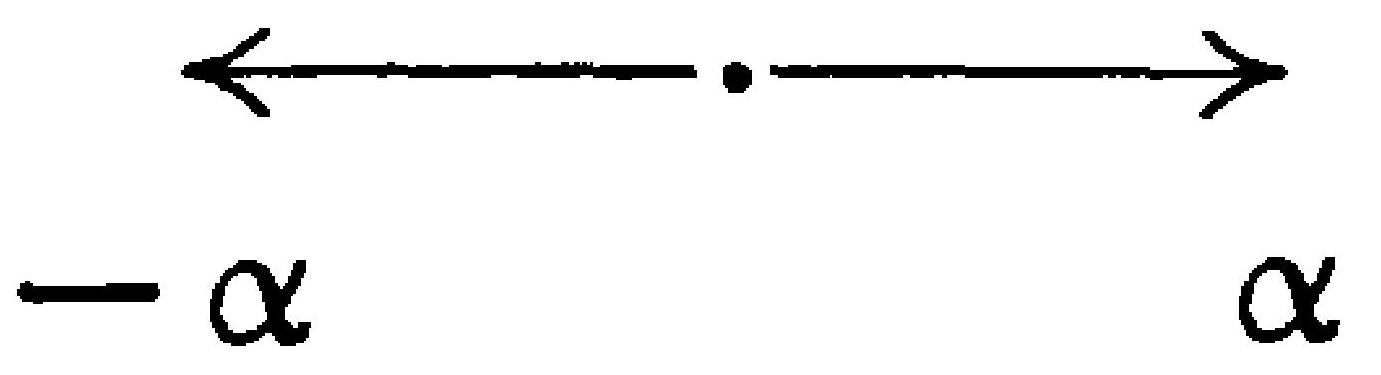
\includegraphics[max width=\textwidth, center]{2025_06_06_fac2836a92464059da43g-056}

Of course, this actually is a root system (with Weyl group of order 2); in Lie algebra theory it belongs to $\mathfrak{s l}(2, \mathrm{~F})$.

Rank 2 offers more possibilities, four of which are depicted in Figure 1 (these turn out to be the only possibilities). In each case the reader should check the axioms directly and determine $\mathscr{W}$.\\
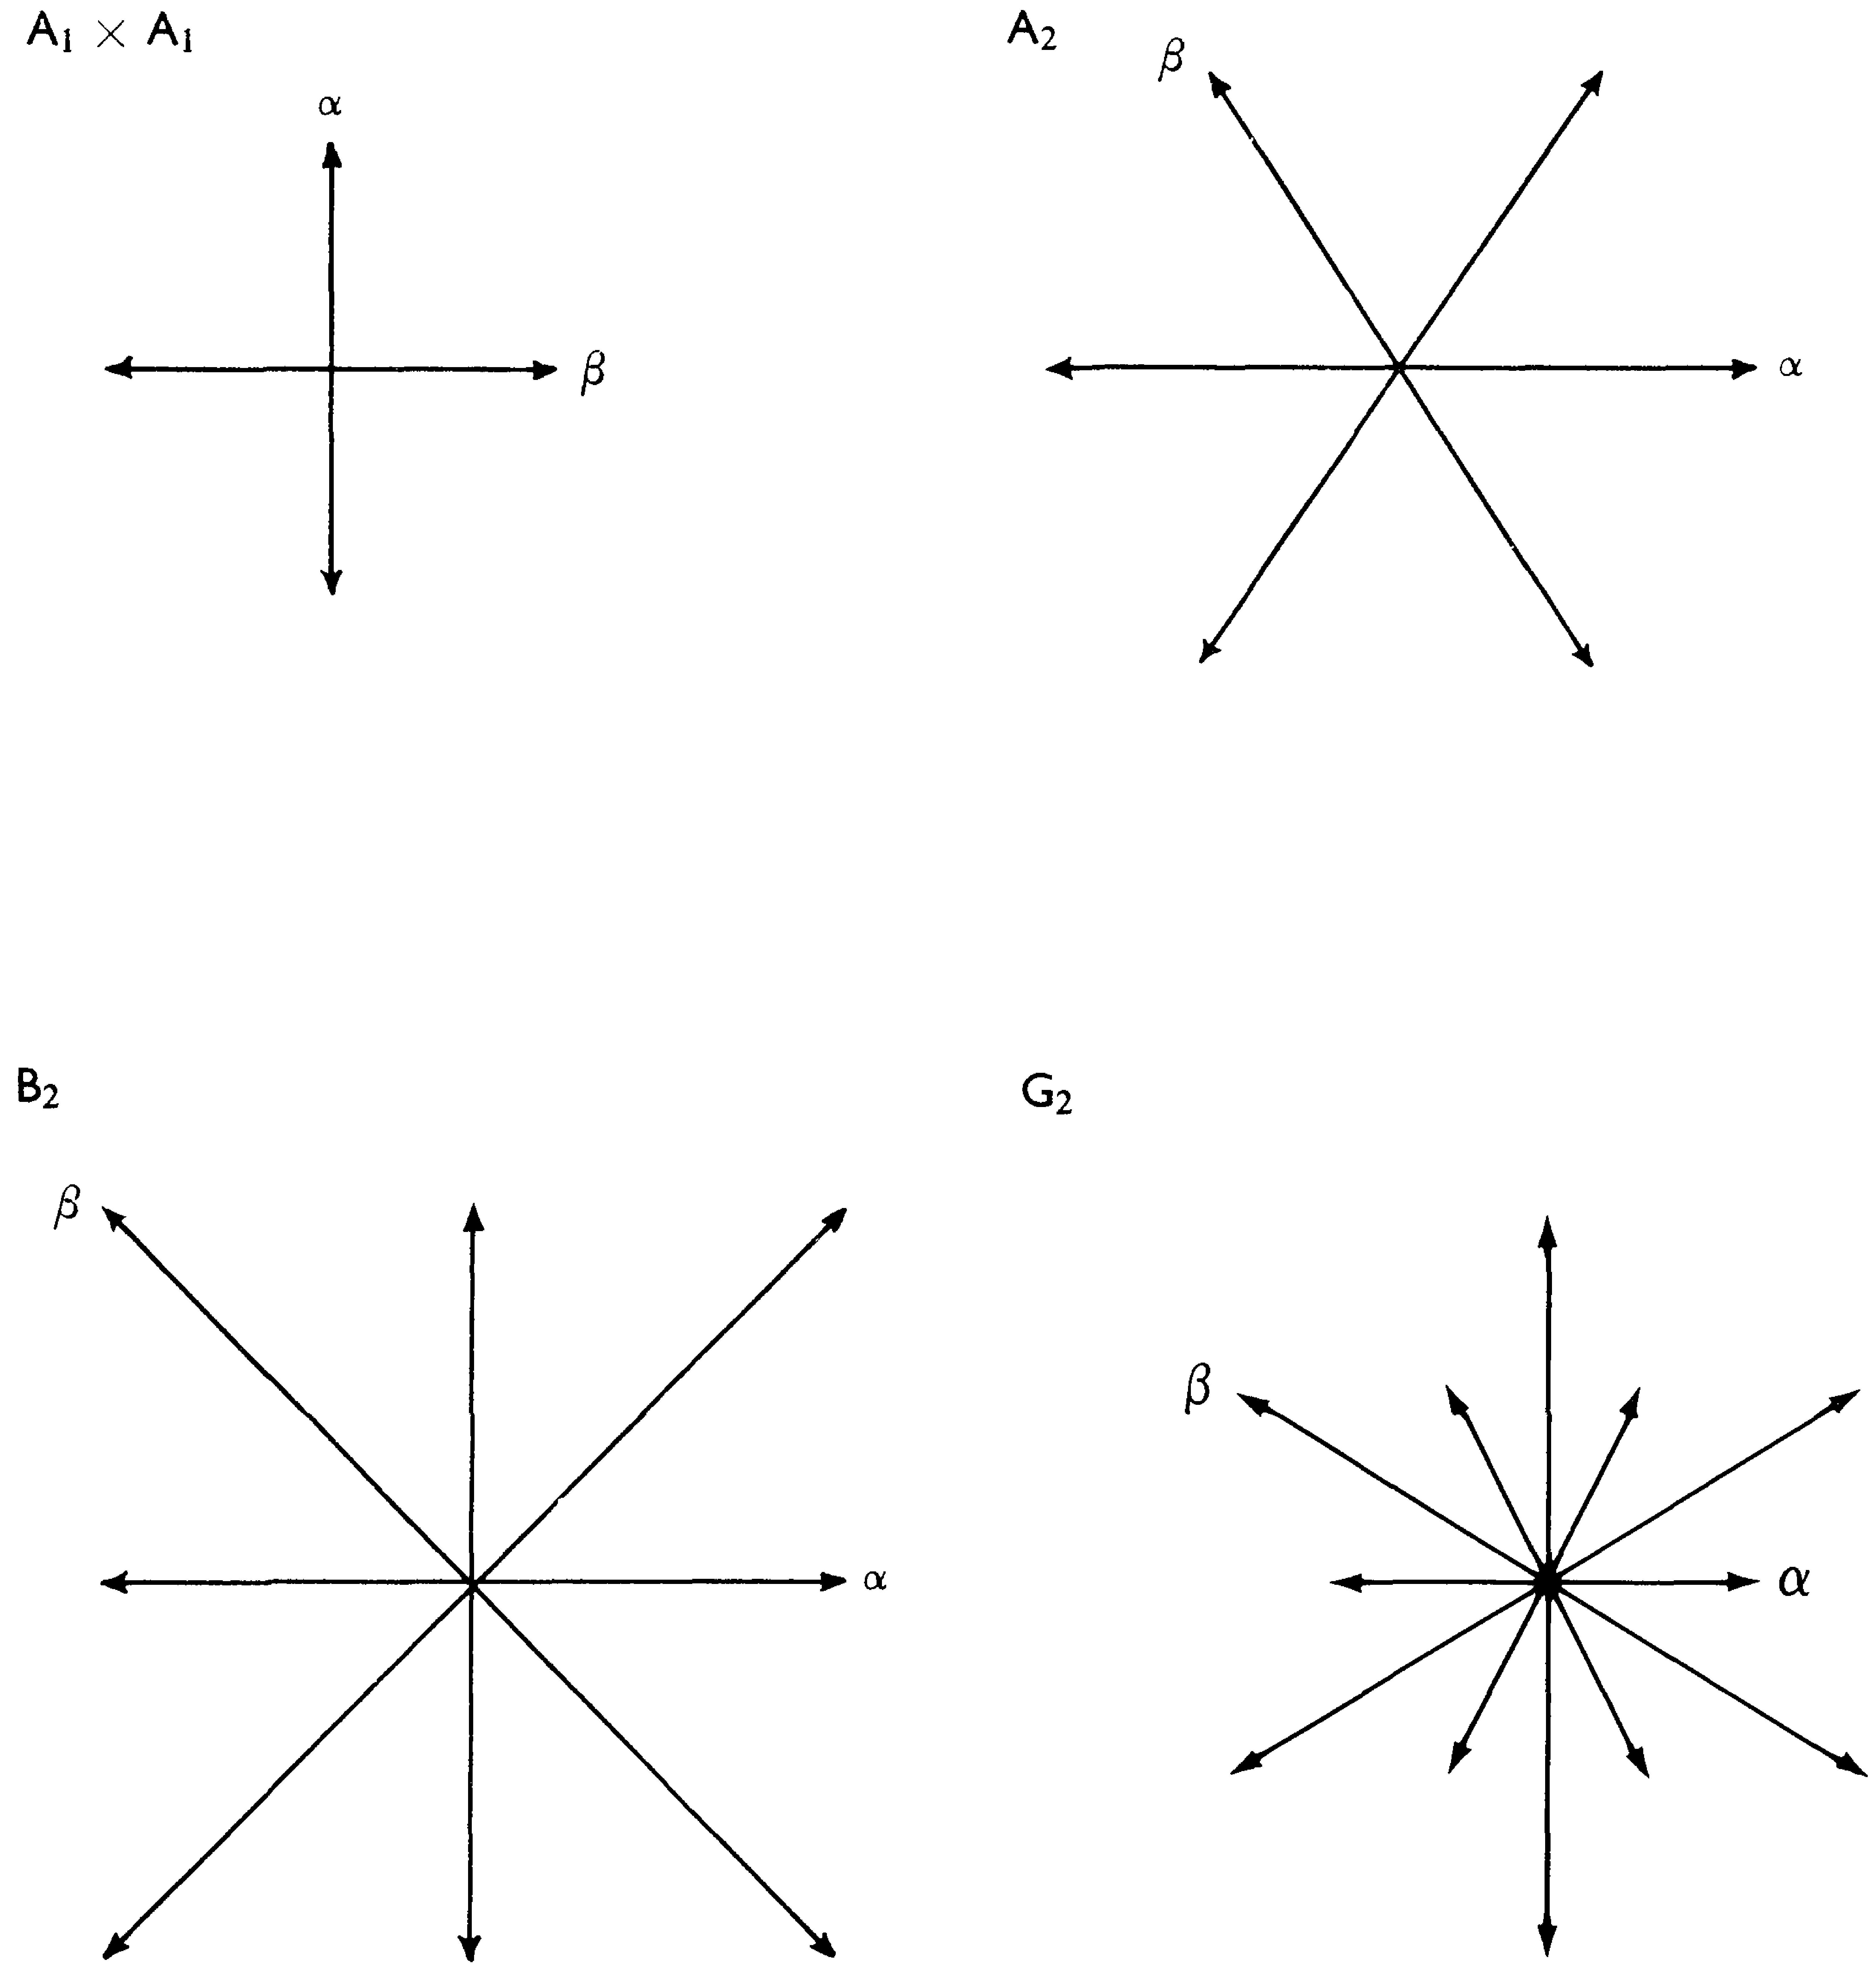
\includegraphics[max width=\textwidth, center]{2025_06_06_fac2836a92464059da43g-057}

Figure 1

\subsection*{9.4. Pairs of roots}
Axiom (R4) limits severely the possible angles occurring between pairs of roots. Recall that the cosine of the angle $\theta$ between vectors $\alpha, \beta \in \mathrm{E}$ is given by the formula $\|\alpha\|\|\beta\| \cos \theta=(\alpha, \beta)$. Therefore, $\langle\beta, \alpha\rangle=\frac{2(\beta, \alpha)}{(\alpha, \alpha)}=$ $2 \frac{\|\beta\|}{\|\alpha\|} \cos \theta$ and $\langle\alpha, \beta\rangle\langle\beta, \alpha\rangle=4 \cos ^{2} \theta$. This last number is a nonnegative integer; but $0 \leq \cos ^{2} \theta \leq 1$, and $\langle\alpha, \beta\rangle,\langle\beta, \alpha\rangle$ have like sign, so the following possibilities are the only ones when $\alpha \neq \pm \beta$ and $\|\beta\| \geq\|\alpha\|$ (Table 1).

Table 1.

\begin{center}
\begin{tabular}{rcrc}
\hline
$\langle\alpha, \beta\rangle$ & $\langle\beta, \alpha\rangle$ &  & \multicolumn{1}{c}{$\theta$} \\
\cline { 1 - 2 }\cline { 4 - 5 }
0 & 0 &  & $\|\beta\|^{2} /\|\alpha\|^{2}$ \\
1 & 1 &  & $\pi / 2$ \\
-1 & -1 &  & $2 \pi / 3$ \\
1 & 2 &  & undetermined \\
-1 & -2 &  & $3 \pi / 4$ \\
1 & 3 &  & 1 \\
-1 & -3 &  & $5 \pi / 6$ \\
\hline
\end{tabular}
\end{center}

The reader will observe that these angles and relative lengths are just the ones portrayed in Figure 1 (9.3). (For $A_{1} \times A_{1}$ it is harmless to change scale in one direction so as to insure that $\|\alpha\|=\|\beta\|$.) The following simple but very useful criterion can be read off from Table 1.

Lemma. Let $\alpha, \beta$ be nonproportional roots. If $(\alpha, \beta)>0$ (i.e., if the angle between $\alpha$ and $\beta$ is strictly acute), then $\alpha-\beta$ is a root. If $(\alpha, \beta)<0$, then $\alpha+\beta$ is a root.

Proof. The second assertion follows from the first (applied to $-\beta$ in place of $\beta$ ). Since ( $\alpha, \beta$ ) is positive if and only if $\langle\alpha, \beta\rangle$ is, Table 1 shows that one or the other of $\langle\alpha, \beta\rangle,\langle\beta, \alpha\rangle$ equals 1 . If $\langle\alpha, \beta\rangle=1$, then $\sigma_{\beta}(\alpha)=\alpha-\beta \in$ $\Phi$ (R3); similarly, if $\langle\beta, \alpha\rangle=1$, then $\beta-\alpha \in \Phi$, hence $\sigma_{\beta-\alpha}(\beta-\alpha)=\alpha-\beta \in$ Ф. ㅁ

As an application, consider a pair of nonproportional roots $\alpha, \beta$. Look at all roots of the form $\beta+i \alpha(i \in \mathbf{Z})$, the $\alpha$-string through $\beta$. Let $r, q \in \mathbf{Z}^{+}$ be the largest integers for which $\beta-r \alpha \in \Phi, \beta+q \alpha \in \Phi$ (respectively). If some $\beta+i \alpha \notin \Phi(-r \leq i \leq q)$, we can find $p<s$ in this interval such that $\beta+p \alpha \in \Phi$, $\beta+(p+1) \alpha \notin \Phi, \beta+(s-1) \alpha \notin \Phi, \beta+s \alpha \in \Phi$. But then the lemma implies both $(\alpha, \beta+p \alpha) \geq 0,(\alpha, \beta+s \alpha) \leq 0$. Since $p<s$ and $(\alpha, \alpha)>0$, this is absurd. We conclude that the $\alpha$-string through $\beta$ is unbroken, from $\beta-r \alpha$ to $\beta+q \alpha$. Now $\sigma_{\alpha}$ just adds or subtracts a multiple of $\alpha$ to any root, so this string is invariant under $\sigma_{\alpha}$. Geometrically, it is obvious that $\sigma_{\alpha}$ just reverses the string (the reader can easily supply an algebraic proof). In particular, $\sigma_{\alpha}(\beta+q \alpha)=\beta-r \alpha$. The left side is $\beta-\langle\beta, \alpha\rangle \alpha-q \alpha$, so finally we obtain: $r-q=\langle\beta, \alpha\rangle$ (cf. Proposition 8.4(e)). It follows at once that root strings are of length at most 4 .

\section*{Exercises}
(Unless otherwise specified, $\Phi$ denotes a root system in E , with Weyl group $\mathscr{W}$.)

\begin{enumerate}
  \item Let $E^{\prime}$ be a subspace of $E$. If a reflection $\sigma_{\alpha}$ leaves $E^{\prime}$ invariant, prove that either $\alpha \in \mathrm{E}^{\prime}$ or else $\mathrm{E}^{\prime} \subset P_{\alpha}$.
  \item Prove that $\Phi^{\vee}$ is a root system in $E$, whose Weyl group is naturally isomorphic to $\mathscr{W}$; show also that $\left\langle\alpha^{\vee}, \beta^{\vee}\right\rangle=\langle\beta, \alpha\rangle$, and draw a picture of $\Phi^{\vee}$ in the cases $A_{1}, A_{2}, B_{2}, G_{2}$.
  \item In Table 1, show that the order of $\sigma_{\alpha} \sigma_{\beta}$ in $\mathscr{W}$ is (respectively) $2,3,4,6$ when $\theta=\pi / 2, \pi / 3$ (or $2 \pi / 3$ ), $\pi / 4$ (or $3 \pi / 4$ ), $\pi / 6$ (or $5 \pi / 6$ ). [Note that $\sigma_{\alpha} \sigma_{\beta}=$ rotation through 20.]
  \item Prove that the respective Weyl groups of $A_{1} \times A_{1}, A_{2}, B_{2}, G_{2}$ are dihedral of order $4,6,8,12$. If $\Phi$ is any root system of rank 2 , prove that its Weyl group must be one of these.
  \item Show by example that $\alpha-\beta$ may be a root even when $(\alpha, \beta) \leq 0$ (cf. Lemma 9.4).
  \item Prove that $\mathscr{W}$ is a normal subgroup of Aut $\Phi$ (= group of all isomorphisms of $\Phi$ onto itself).
  \item Let $\alpha, \beta \in \Phi$ span a subspace $E^{\prime}$ of $E$. Prove that $E^{\prime} \cap \Phi$ is a root system in $E^{\prime}$. Prove similarly that $\Phi \cap(\mathbf{Z} \alpha+\mathbf{Z} \beta)$ is a root system in $E^{\prime}$ (must this coincide with $E^{\prime} \cap \Phi$ ?). More generally, let $\Phi^{\prime}$ be a nonempty subset of $\Phi$ such that $\Phi^{\prime}=-\Phi^{\prime}$, and such that $\alpha, \beta \in \Phi^{\prime}, \alpha+\beta \in \Phi$ implies $\alpha+\beta \in \Phi^{\prime}$. Prove that $\Phi^{\prime}$ is a root system in the subspace of E it spans. [Use Table 1].
  \item Compute root strings in $\mathrm{G}_{2}$ to verify the relation $r-q=\langle\beta, \alpha\rangle$.
  \item Let $\Phi$ be a set of vectors in a euclidean space $E$, satisfying only (R1), (R3), (R4). Prove that the only possible multiples of $\alpha \in \Phi$ which can be in $\Phi$ are $\pm 1 / 2 \alpha, \pm \alpha, \pm 2 \alpha$. Verify that $\{\alpha \in \Phi \mid 2 \alpha \notin \Phi\}$ is a root system. Example: See Figure 2.\\
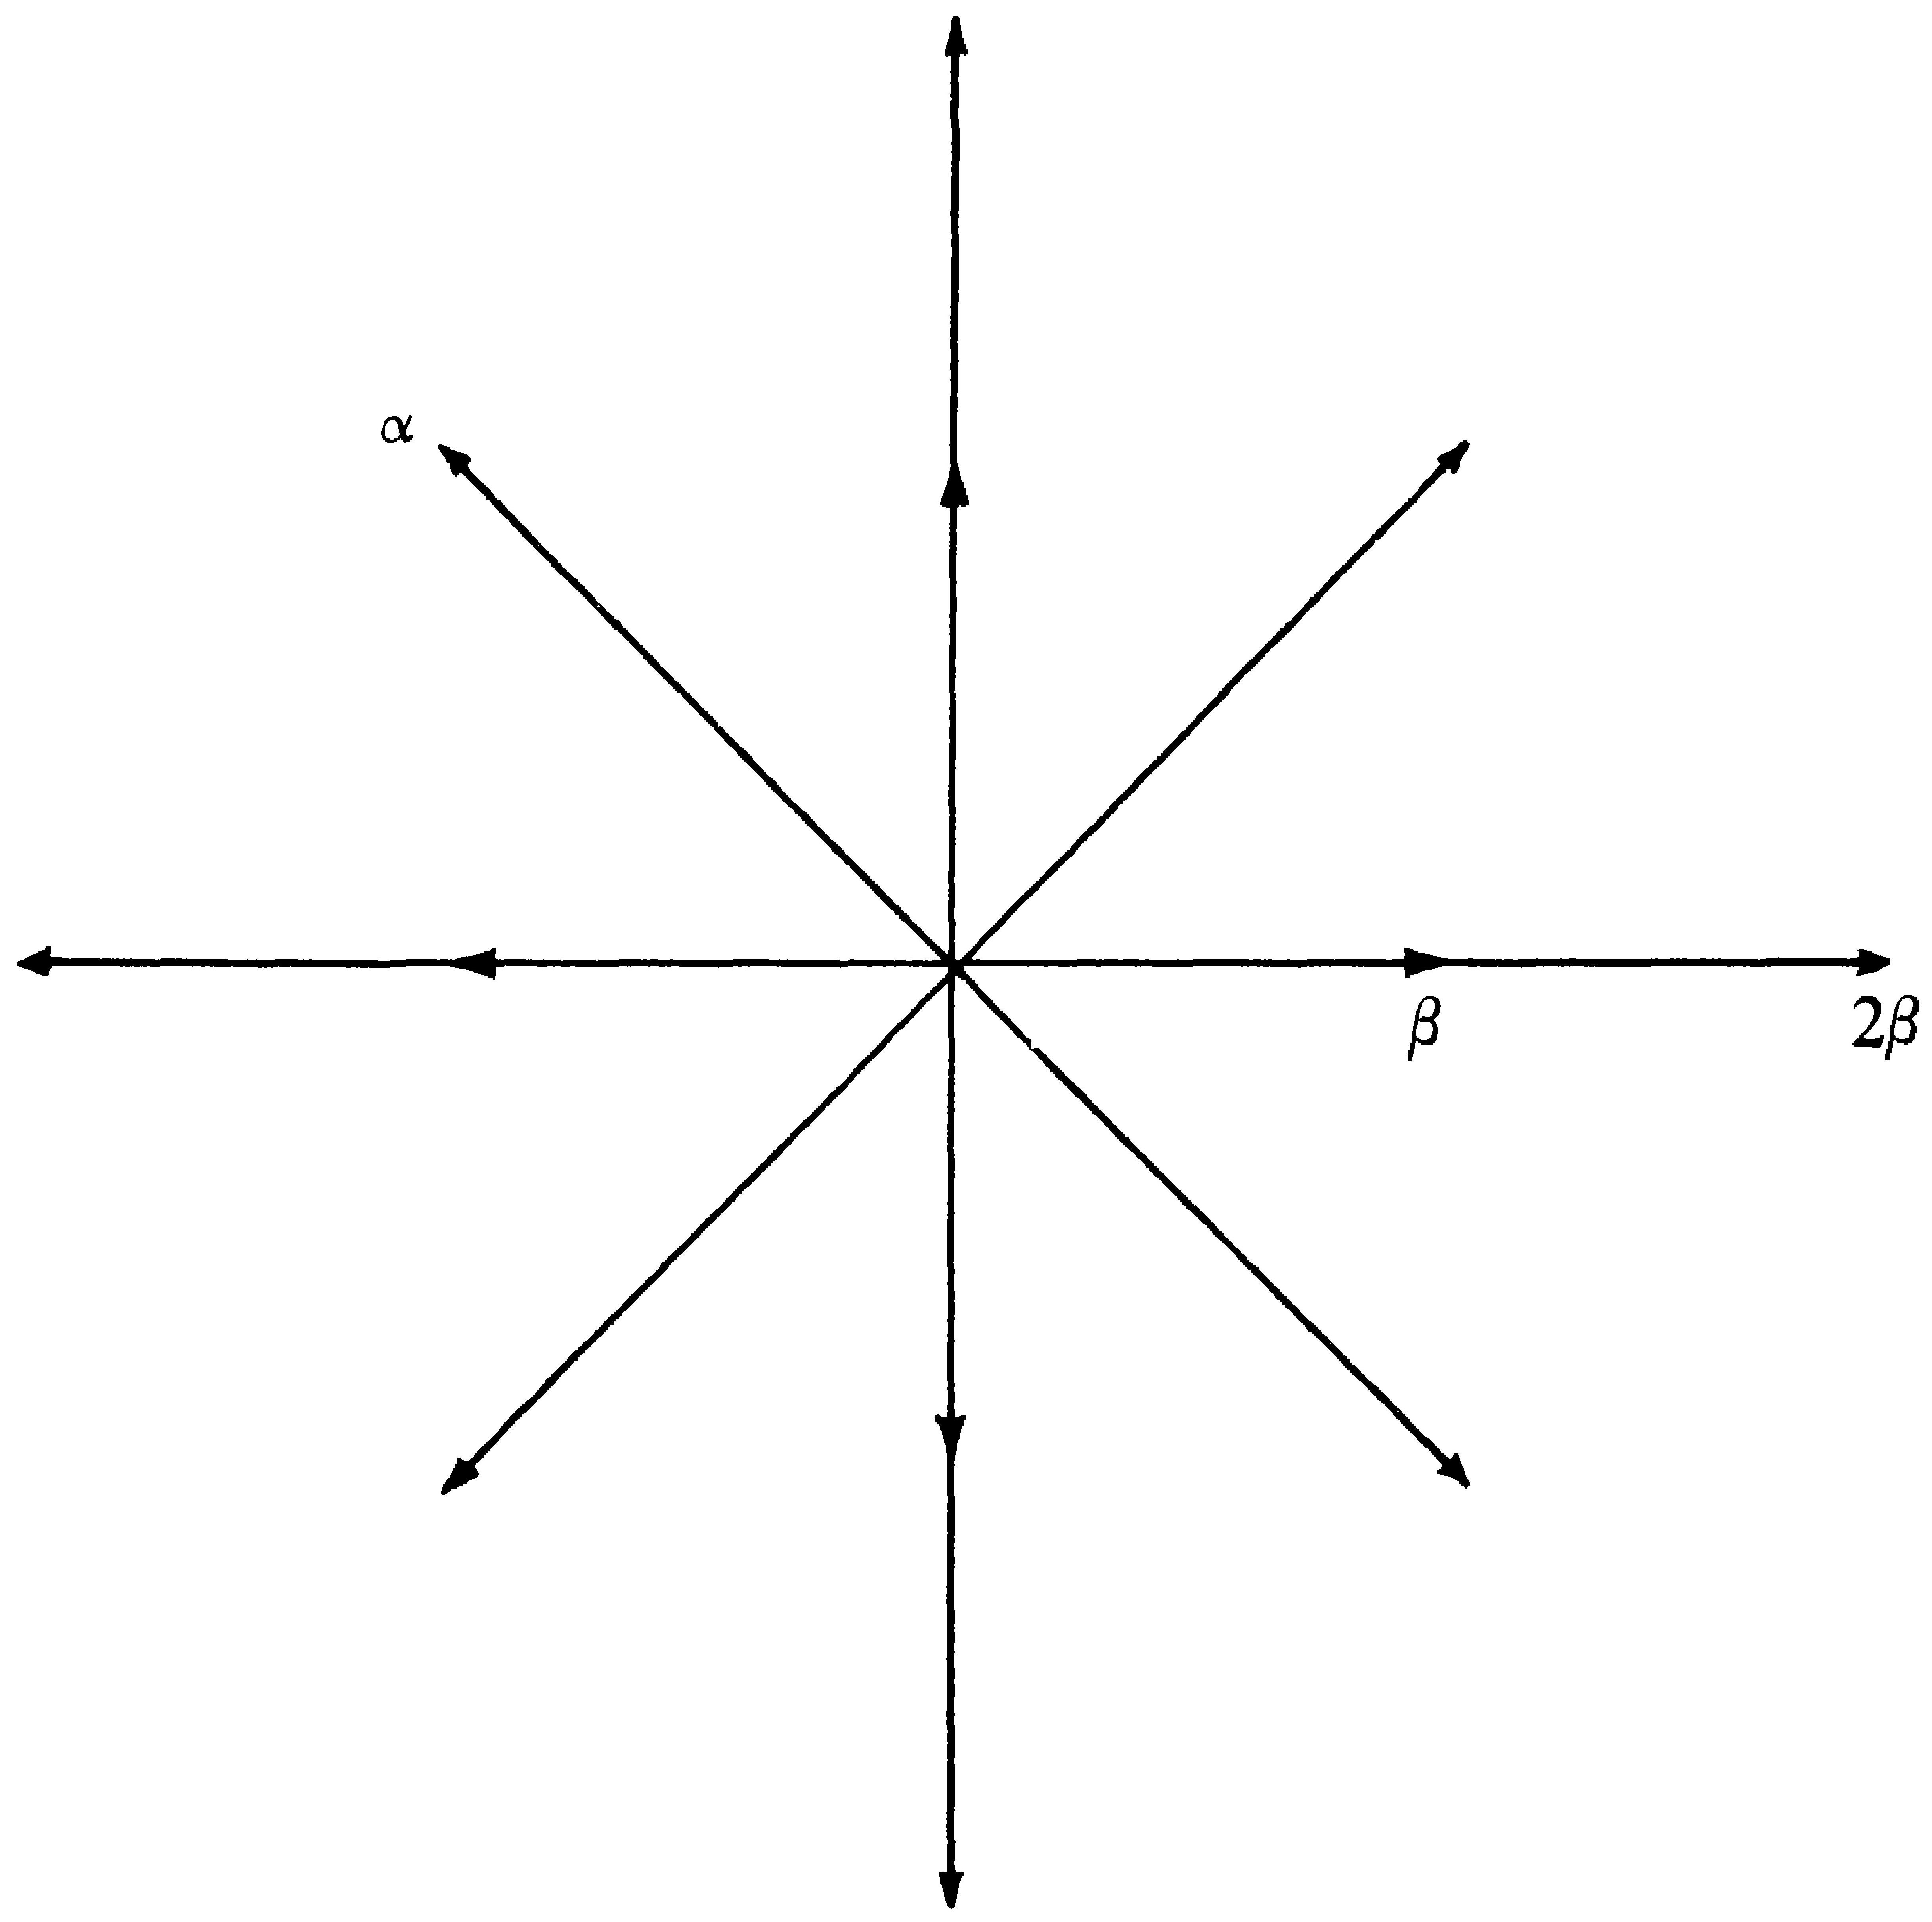
\includegraphics[max width=\textwidth, center]{2025_06_06_fac2836a92464059da43g-059}
\end{enumerate}

Figure 2\\
10. Let $\alpha, \beta \in \Phi$. Let the $\alpha$-string through $\beta$ be $\beta-r \alpha, \ldots, \beta+q \alpha$, and let the $\beta$-string through $\alpha$ be $\alpha-r^{\prime} \beta, \ldots, \alpha+q^{\prime} \beta$. Prove that $\frac{q(r+1)}{(\beta, \beta)}=\frac{q^{\prime}\left(r^{\prime}+1\right)}{(\alpha, \alpha)}$.\\
11. Let $c$ be a positive real number. If $\Phi$ possesses any roots of squared length $c$, prove that the set of all such roots is a root system in the subspace of E it spans. Describe the possibilities occurring in Figure 1.

\section*{Notes}
The axiomatic approach to root systems (as in Serre [2], Bourbaki [2]) has the advantage of providing results which apply simultaneously to Lie algebras, Lie groups, and linear algebraic groups. For historical remarks, consult Bourbaki [2].

\section*{10. Simple roots and Weyl group}
Throughout this section $\Phi$ denotes a root system of rank $\ell$ in a euclidean space E , with Weyl group $\mathscr{W}^{\sim}$.

\subsection*{10.1. Bases and Weyl chambers}
A subset $\Delta$ of $\Phi$ is called a base if:\\
(B1) $\Delta$ is a basis of $E$,\\
(B2) each root $\beta$ can be written as $\beta=\sum k_{\alpha} \alpha(\alpha \in \Delta)$ with integral coefficients $k_{\alpha}$ all nonnegative or all nonpositive.\\
The roots in $\Delta$ are then called simple. In view of (B1), Card $\Delta=\ell$, and the expression for $\beta$ in (B2) is unique. This allows us to define the height of a root (relative to $\Delta$ ) by ht $\beta=\sum_{\alpha \in \Delta} k_{\alpha}$. If all $k_{\alpha} \geq 0$ (resp. all $k_{\alpha} \leq 0$ ), we call $\beta$ positive (resp. negative) and write $\beta \succ 0$ (resp. $\beta \prec 0$ ). The collections of positive and negative roots (relative to $\Delta$ ) will usually just be denoted $\Phi^{+}$ and $\Phi^{-}$(clearly, $\Phi^{-}=-\Phi^{+}$). If $\alpha$ and $\beta$ are positive roots, and $\alpha+\beta$ is a root, then evidently $\alpha+\beta$ is also positive. Actually, $\Delta$ defines a partial order on E , compatible with the notation $\alpha \succ 0$ : define $\beta \prec \alpha$ iff $\alpha-\beta$ is a sum of positive roots (equivalently, of simple roots) or $\beta=\alpha$.

The only problem with the definition of base is that it fails to guarantee existence. In the examples shown in (9.3), the roots labelled $\alpha, \beta$ do form a base in each case (verify!). Notice there that the angle between $\alpha$ and $\beta$ is obtuse, i.e., $(\alpha, \beta) \leq 0$. This is no accident.

Lemma. If $\Delta$ is a base of $\Phi$, then $(\alpha, \beta) \leq 0$ for $\alpha \neq \beta$ in $\Delta$, and $\alpha-\beta$ is not a root.

Proof. Otherwise $(\alpha, \beta)>0$. Since $\alpha \neq \beta$, by assumption, and since obviously $\alpha \neq-\beta$, Lemma 9.4 then says that $\alpha-\beta$ is a root. But this violates (B2).

Our goal is the proof of the following theorem.\\
Theorem. $\Phi$ has a base.\\
The proof will in fact yield a concrete method for constructing all possible bases. For each vector $\gamma \in \mathrm{E}$, define $\Phi^{+}(\gamma)=\{\alpha \in \Phi \mid(\gamma, \alpha)>0\}=$ the set of roots lying on the "positive" side of the hyperplane orthogonal to $\gamma$. It is an elementary fact in euclidean geometry that the union of the finitely many hyperplanes $P_{\alpha}(\alpha \in \Phi)$ cannot exhaust E (we leave to the reader the task of formulating a rigorous proof). Call $\gamma \in \mathrm{E}$ regular if $\gamma \in \mathrm{E}-\bigcup_{\alpha \in \Phi} P_{\alpha}$, singular otherwise. When $\gamma$ is regular, it is clear that $\Phi=\Phi^{+}(\gamma) \cup-\Phi^{+}(\gamma)$. This is the case we shall now pursue. Call $\alpha \in \Phi^{+}(\gamma)$ decomposable if $\alpha=$ $\beta_{1}+\beta_{2}$ for some $\beta_{i} \in \Phi^{+}(\gamma)$, indecomposable otherwise. Now it suffices to prove the following statement.

Theorem'. Let $\gamma \in \mathrm{E}$ be regular. Then the set $\Delta(\gamma)$ of all indecomposable roots in $\Phi^{+}(\gamma)$ is a base of $\Phi$, and every base is obtainable in this manner.

Proof. This will proceed in steps.\\
(1) Each root in $\Phi^{+}(\gamma)$ is a nonnegative $\mathbf{Z}$-linear combination of $\Delta(\gamma)$. Otherwise some $\alpha \in \Phi^{+}(\gamma)$ cannot be so written; choose $\alpha$ so that ( $\gamma, \alpha$ ) is as small as possible. Obviously $\alpha$ itself cannot be in $\Delta(\gamma)$, so $\alpha=\beta_{1}+\beta_{2}$ $\left(\beta_{i} \in \Phi^{+}(\gamma)\right)$, whence $(\gamma, \alpha)=\left(\gamma, \beta_{1}\right)+\left(\gamma, \beta_{2}\right)$. But each of the $\left(\gamma, \beta_{i}\right)$ is positive, so $\beta_{1}$ and $\beta_{2}$ must each be a nonnegative Z-linear combination of $\Delta(\gamma)$ (to avoid contradicting the minimality of ( $\gamma, \alpha$ )), whence $\alpha$ also is. This contradiction proves the original assertion.\\
(2) If $\alpha, \beta \in \Delta(\gamma)$, then $(\alpha, \beta) \leq 0$ unless $\alpha=\beta$. Otherwise $\alpha-\beta$ is a root (Lemma 9.4), since $\beta$ clearly cannot be $-\alpha$, so $\alpha-\beta$ or $\beta-\alpha$ is in $\Phi^{+}(\gamma)$. In the first case, $\alpha=\beta+(\alpha-\beta)$, which says that $\alpha$ is decomposable; in the second case, $\beta=\alpha+(\beta-\alpha)$ is decomposable. This contradicts the assumption.\\
(3) $\Delta(\gamma)$ is a linearly independent set. Suppose $\Sigma r_{\alpha} \alpha=0\left(\alpha \in \Delta(\gamma), r_{\alpha} \in \mathbb{R}\right)$. Separating the indices $\alpha$ for which $r_{\alpha}>0$ from those for which $r_{\alpha}<0$, we can rewrite this as $\Sigma s_{\alpha}=\Sigma t_{\beta} \beta$ ( $s_{\alpha}, t_{\beta}>0$, the sets of $\alpha$ 's and $\beta$ 's being disjoint). Call $\varepsilon=\Sigma S_{\alpha} \alpha$. Then ( $\varepsilon, \varepsilon$ ) $=\sum_{\alpha, \beta} S_{\alpha} t_{\beta}(\alpha, \beta) \leq 0$ by step (2), forcing $\varepsilon=0$. Then $0=(\gamma, \varepsilon)=\Sigma s_{\alpha}(\gamma, \alpha)$, forcing all $s_{\alpha}=0$. Similarly, all $t_{\beta}=0$. (This argument actually shows that any set of vectors lying strictly on one side of a hyperplane in E and forming pairwise obtuse angles must be linearly independent.)\\
(4) $\Delta(\gamma)$ is a base of $\Phi$. Since $\Phi=\Phi^{+}(\gamma) \cup-\Phi^{+}(\gamma)$, the requirement (B2) is satisfied thanks to step (1). It also follows that $\Delta(\gamma)$ spans E , which combined with step (3) yields (B1).\\
(5) Each base $\Delta$ of $\Phi$ has the form $\Delta(\gamma)$ for some regular $\gamma \in \mathrm{E}$. Given $\Delta$, select $\gamma \in \mathrm{E}$ so that $(\gamma, \alpha)>0$ for all $\alpha \in \Delta$. (This is possible, because the intersection of "positive" open half-spaces associated with any basis of E is nonvoid (Exercise 7).) In view of (B2), $\gamma$ is regular and $\Phi^{+} \subset \Phi^{+}(\gamma)$, $\Phi^{-} \subset-\Phi^{+}(\gamma)$ (so equality must hold in each instance). Since $\Phi^{+}=\Phi^{+}(\gamma)$,\\
$\Delta$ clearly consists of indecomposable elements, i.e., $\Delta \subset \Delta(\gamma)$. But Card $\Delta=$ Card $\Delta(\gamma)=\ell$, so $\Delta=\Delta(\gamma)$. $\square$

It is useful to introduce a bit of terminology. The hyperplanes $P_{\alpha}(\alpha \in \Phi)$ partition E into finitely many regions; the connected components of $\mathrm{E}-\bigcup_{\alpha} P_{\alpha}$ are called the (open) Weyl chambers of E. Each regular $\gamma \in \mathrm{E}$ therefore belongs to precisely one Weyl chamber, denoted $\mathfrak{C}(\gamma)$. To say that $\mathfrak{C}(\gamma)=\mathfrak{C}\left(\gamma^{\prime}\right)$ is just to say that $\gamma, \gamma^{\prime}$ lie on the same side of each hyperplane $P_{\alpha}(\alpha \in \Phi)$, i.e., that $\Phi^{+}(\gamma)=\Phi^{+}\left(\gamma^{\prime}\right)$, or $\Delta(\gamma)=\Delta\left(\gamma^{\prime}\right)$. This shows that Weyl chambers are in natural 1-1 correspondence with bases. Write $\mathfrak{C}(\Delta)=\mathfrak{C}(\gamma)$ if $\Delta=\Delta(\gamma)$, and call this the fundamental Weyl chamber relative to $\Delta$. $\mathfrak{C}(\Delta)$ is the open convex set (intersection of open half-spaces) consisting of all $\gamma \in \mathrm{E}$ which satisfy the inequalities $(\gamma, \alpha)>0(\alpha \in \Delta)$. In rank 2 , it is easy to draw the appropriate picture; this is done in Figure 1 for type $A_{2}$. Here there are six chambers, the shaded one being fundamental relative to the base $\{\alpha, \beta\}$.

The Weyl group obviously sends one Weyl chamber onto another: explicitly, $\sigma(\mathcal{C}(\gamma))=\mathfrak{C}(\sigma \gamma)$, if $\sigma \in \mathscr{W}$ and $\gamma$ is regular. On the other hand, $\mathscr{W}$ permutes bases: $\sigma$ sends $\Delta$ to $\sigma(\Delta)$, which is again a base (why?). These two actions of $\mathscr{W}$ are in fact compatible with the above correspondence\\
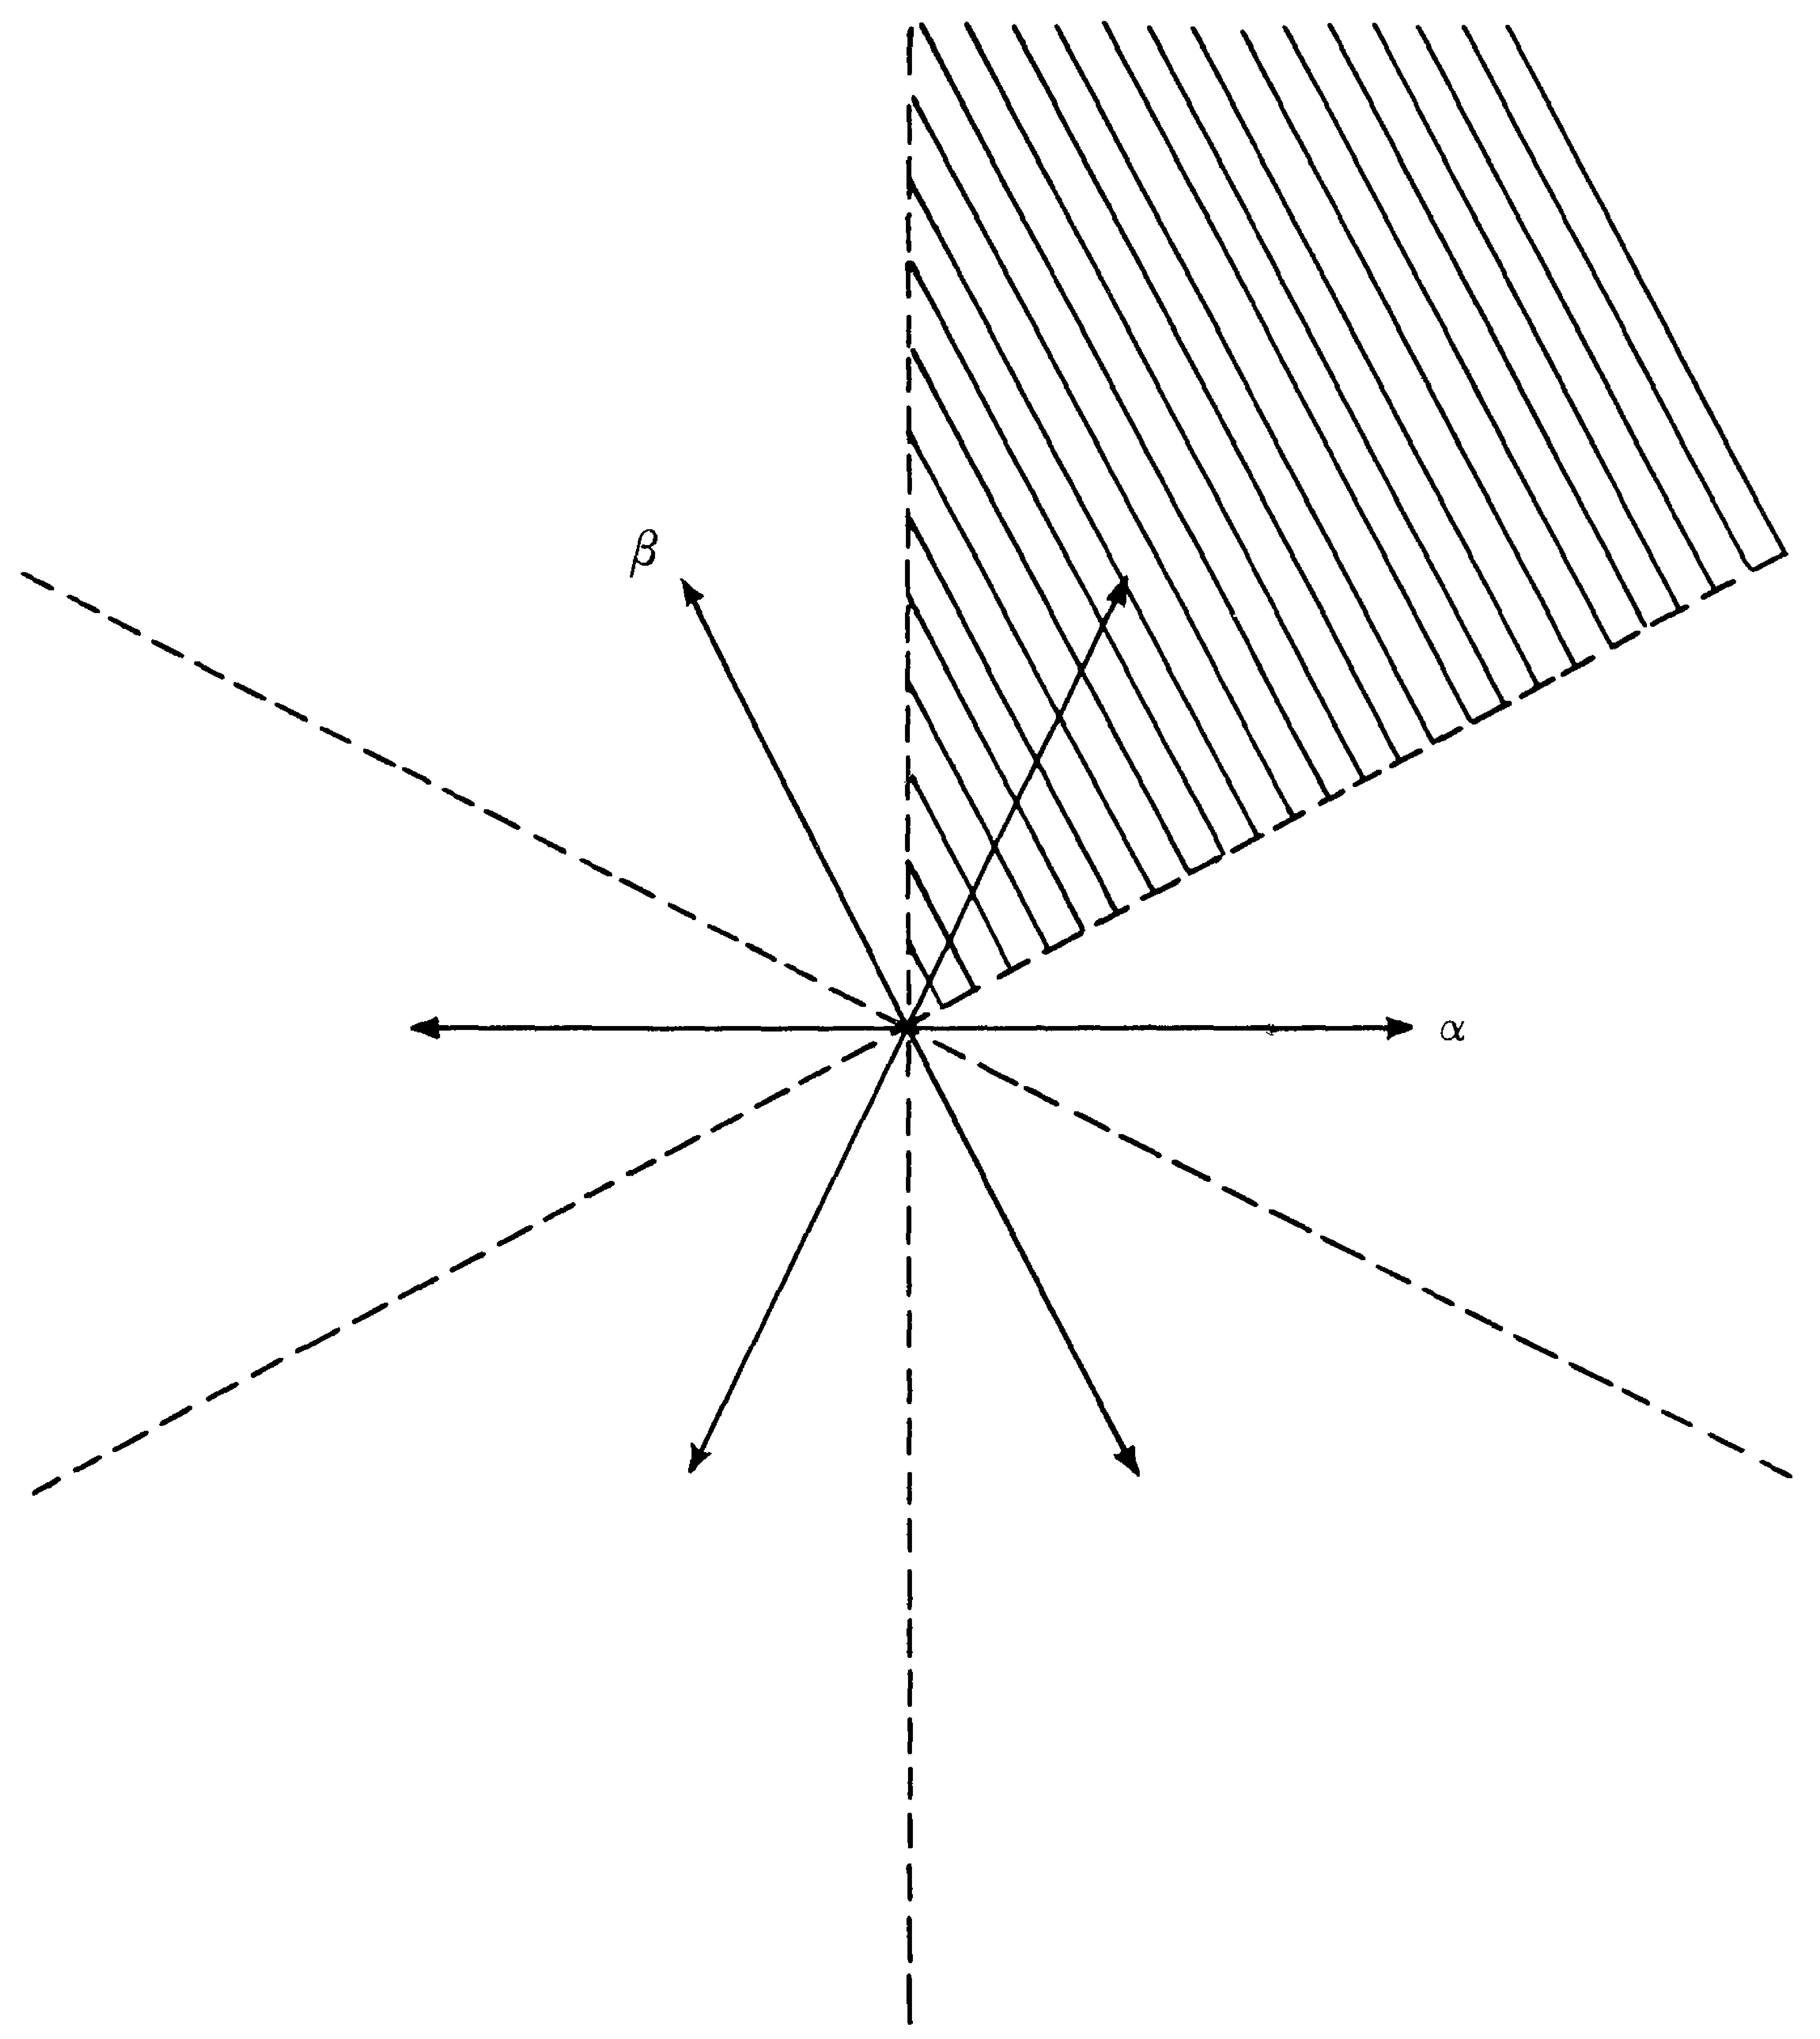
\includegraphics[max width=\textwidth, center]{2025_06_06_fac2836a92464059da43g-062}

Figure 1\\
between Weyl chambers and bases; we have $\sigma(\Delta(\gamma))=\Delta(\sigma \gamma)$, because $(\sigma \gamma, \sigma \alpha)=(\gamma, \alpha)$.

\subsection*{10.2. Lemmas on simple roots}
Let $\Delta$ be a fixed base of $\Phi$. We prove here several very useful lemmas about the behavior of simple roots.

Lemma A. If $\alpha$ is positive but not simple, then $\alpha-\beta$ is a root (necessarily positive) for some $\beta \in \Delta$.

Proof. If $(\alpha, \beta) \leq 0$ for all $\beta \in \Delta$, the parenthetic remark in step (3) in (10.1) would apply, showing that $\Delta \cup\{\alpha\}$ is a linearly independent set. This is absurd, since $\Delta$ is already a basis of E . So $(\alpha, \beta)>0$ for some $\beta \in \Delta$ and then $\alpha-\beta \in \Phi$ (Lemma 9.4, which applies since $\beta$ cannot be proportional to $\alpha$ ). Write $\alpha=\sum_{\gamma \in \Delta} k_{\gamma} \gamma\left(\right.$ all $k_{\gamma} \geq 0$, some $k_{\gamma}>0$ for $\gamma \neq \beta$ ). Subtracting $\beta$ from $\alpha$ yields a Z-linear combination of simple roots with at least one positive coefficient. This forces all coefficients to be positive, thanks to the uniqueness of expression in (B2).

Corollary. Each $\beta \in \Phi^{+}$can be written in the form $\alpha_{1}+\ldots+\alpha_{k}\left(\alpha_{i} \in \Delta\right.$, not necessarily distinct) in such a way that each partial sum $\alpha_{1}+\ldots+\alpha_{i}$ is a root.

Proof. Use the lemma and induction on ht $\beta$.\\
Lemma B. Let $\alpha$ be simple. Then $\sigma_{\alpha}$ permutes the positive roots other than $\alpha$.\\
Proof. Let $\beta \in \Phi^{+}-\{\alpha\}, \beta=\sum_{\gamma \in \Delta} k_{\gamma} \gamma\left(k_{\gamma} \in \mathbf{Z}^{+}\right)$. It is clear that $\beta$ is not proportional to $\alpha$. Therefore, $k_{\gamma} \neq 0$ for some $\gamma \neq \alpha$. But the coefficient of $\gamma$ in $\sigma_{\alpha}(\beta)=\beta-\langle\beta, \alpha\rangle \alpha$ is still $k_{\gamma}$. In other words, $\sigma_{\alpha}(\beta)$ has at least one positive coefficient (relative to $\Delta$ ), forcing it to be positive. Moreover, $\sigma_{\alpha}(\beta) \neq \alpha$, since $\alpha$ is the image of $-\alpha$.

Corollary. Set $\delta=\frac{1}{2} \sum_{\beta>0} \beta$. Then $\sigma_{\alpha}(\delta)=\delta-\alpha$ for all $\alpha \in \Delta$.\\
Proof. Obvious from the lemma.\\
Lemma C. Let $\alpha_{1}, \ldots, \alpha_{t} \in \Delta$ (not necessarily distinct). Write $\sigma_{i}=\sigma_{\alpha_{i}}$. If $\sigma_{1} \ldots \sigma_{t-1}\left(\alpha_{t}\right)$ is negative, then for some index $1 \leq s<t, \sigma_{1} \ldots \sigma_{t}=$ $\sigma_{1} \ldots \sigma_{s-1} \sigma_{s+1} \ldots \sigma_{t-1}$.

Proof. Write $\beta_{i}=\sigma_{i+1} \ldots \sigma_{t-1}\left(\alpha_{t}\right), \quad 0 \leq i \leq t-2, \quad \beta_{t-1}=\alpha_{t}$. Since $\beta_{0} \prec 0$ and $\beta_{t-1} \succ 0$, we can find a smallest index $s$ for which $\beta_{s} \succ 0$. Then $\sigma_{s}\left(\beta_{s}\right)=\beta_{s-1} \prec 0$, and Lemma B forces $\beta_{s}=\alpha_{s}$. In general (Lemma 9.2), $\sigma \in \mathscr{W}$ implies $\sigma_{\sigma(\alpha)}=\sigma \sigma_{\alpha} \sigma^{-1}$; so in particular, $\sigma_{s}=\left(\sigma_{s+1} \ldots \sigma_{t-1}\right) \sigma_{t}$ ( $\sigma_{t-1} \ldots \sigma_{s+1}$ ) which yields the lemma.

Corollary. If $\sigma=\sigma_{1} \ldots \sigma_{t}$ is an expression for $\sigma \in \mathscr{W}$ in terms of reflections corresponding to simple roots, with $t$ as small as possible, then $\sigma\left(\alpha_{t}\right) \prec 0$.

\subsection*{10.3. The Weyl group}
Now we are in a position to prove that $\mathscr{W}$ permutes the bases of $\Phi$ (or, equivalently, the Weyl chambers) in a simply transitive fashion and that $\mathscr{W}$ is generated by the "simple reflections" relative to any base $\Delta$ (i.e., by the $\sigma_{\alpha}$ for $\alpha \in \Delta$ ).

Theorem. Let $\Delta$ be a base of $\Phi$.\\
(a) If $\gamma \in \mathrm{E}, \gamma$ regular, there exists $\sigma \in \mathscr{W}$ such that $(\sigma(\gamma), \alpha)>0$ for all $\alpha \in \Delta$ (so $\mathscr{W}$ acts transitively on Weyl chambers).\\
(b) If $\Delta^{\prime}$ is another base of $\Phi$, then $\sigma\left(\Delta^{\prime}\right)=\Delta$ for some $\sigma \in \mathscr{W}$ (so $\mathscr{W}$ acts transitively on bases).\\
(c) If $\alpha$ is any root, there exists $\sigma \in \mathscr{W}$ such that $\sigma(\alpha) \in \Delta$.\\
(d) $\mathscr{W}$ is generated by the $\sigma_{\alpha}(\alpha \in \Delta)$.\\
(e) If $\sigma(\Delta)=\Delta, \sigma \in \mathscr{W}$, then $\sigma=1$ (so $\mathscr{W}$ acts simply transitively on bases).

Proof. Let $\mathscr{W}^{\prime}$ be the subgroup of $\mathscr{W}$ generated by all $\sigma_{\alpha}(\alpha \in \Delta)$. We shall prove (a)-(c) for $\mathscr{W}^{\prime}$, then deduce that $\mathscr{W}^{\prime}=\mathscr{W}$.\\
(a) Write $\delta=\frac{1}{2} \sum_{\alpha>0} \alpha$, and choose $\sigma \in \mathscr{W}^{\prime}$ for which $(\sigma(\gamma), \delta)$ is as big as possible. If $\alpha$ is simple, then of course $\sigma_{\alpha} \sigma$ is also in $\mathscr{W}^{\prime}$, so the choice of $\sigma$ implies that $(\sigma(\gamma), \delta) \geq\left(\sigma_{\alpha} \sigma(\gamma), \delta\right)=\left(\sigma(\gamma), \sigma_{\alpha}(\delta)\right)=(\sigma(\gamma), \delta-\alpha)=(\sigma(\gamma), \delta)$ $-(\sigma(\gamma), \alpha)$ (Corollary to Lemma 10.2B). This forces $(\sigma(\gamma), \alpha) \geq 0$ for all $\alpha \in \Delta$. Since $\gamma$ is regular, we cannot have $(\sigma(\gamma), \alpha)=0$ for any $\alpha$, because then $\gamma$ would be orthogonal to $\sigma^{-1} \alpha$. So all the inequalities are strict. Therefore $\sigma(\gamma)$ lies in the fundamental Weyl chamber $\mathcal{C}(\Delta)$, and $\sigma$ sends $\mathcal{C}(\gamma)$ to $\mathfrak{C}(\Delta)$ as desired.\\
(b) Since $\mathscr{W}^{\prime}$ permutes the Weyl chambers, by (a), it also permutes the bases of $\Phi$ (transitively).\\
(c) In view of (b), it suffices to prove that each root belongs to at least one base. Since the only roots proportional to $\alpha$ are $\pm \alpha$, the hyperplanes $P_{\beta}(\beta \neq \pm \alpha)$ are distinct from $P_{\alpha}$, so there exists $\gamma \in P_{\alpha}, \gamma \neq P_{\beta}$ (all $\beta \neq \pm \alpha$ ) (why?). Choose $\gamma^{\prime}$ close enough to $\gamma$ so that $\left(\gamma^{\prime}, \alpha\right)=\varepsilon>0$ while $\left|\left(\gamma^{\prime}, \beta\right)\right|>\varepsilon$ for all $\beta \neq \pm \alpha$. Evidently $\alpha$ then belongs to the base $\Delta\left(\gamma^{\prime}\right)$.\\
(d) To prove $\mathscr{W}^{\prime}=\mathscr{W}$, it is enough to show that each reflection $\sigma_{\alpha}$ $(\alpha \in \Phi)$ is in $\mathscr{W}^{\prime}$. Using (c); find $\sigma \in \mathscr{W}^{\prime}$ such that $\beta=\sigma(\alpha) \in \Delta$. Then $\sigma_{\beta}=$ $\sigma_{\sigma(\alpha)}=\sigma \sigma_{\alpha} \sigma^{-1}$, so $\sigma_{\alpha}=\sigma^{-1} \sigma_{\beta} \sigma \in \mathscr{W}^{\prime \prime}$.\\
(e) Let $\sigma(\Delta)=\Delta$, but $\sigma \neq 1$. If $\sigma$ is written minimally as a product of one or more simple reflections (which is possible, thanks to (d)), then the Corollary to Lemma 10.2C is contradicted.

We can use the lemmas of (10.2) to explore more precisely the significance of the generation of $\mathscr{W}$ by simple reflections.

When $\sigma \in \mathscr{W}$ is written as $\sigma_{\alpha_{1}} \ldots \sigma_{\alpha_{t}}\left(\alpha_{i} \in \Delta, t\right.$ minimal), we call the expression reduced, and write $t(\sigma)=t$ : this is the length of $\sigma$, relative to $\Delta$. By definition, $\ell(1)=0$. We can characterize length in another way, as follows. Define $n(\sigma)=$ number of positive roots $\alpha$ for which $\sigma(\alpha) \prec 0$.

Lemma A. For all $\sigma \in \mathscr{W}, \ell(\sigma)=n(\sigma)$.\\
Proof. Proceed by induction on $\ell(\sigma)$. The case $\ell(\sigma)=0$ is clear: $\ell(\sigma)=0$ implies $\sigma=1$, so $n(\sigma)=0$. Assume the lemma true for all $\tau \in \mathscr{W}$ with $\ell(\tau)<\ell(\sigma)$. Write $\sigma$ in reduced form as $\sigma=\sigma_{\alpha_{1}} \ldots \sigma_{\alpha_{t}}$, and set $\alpha=\alpha_{t}$. By the Corollary of Lemma 10.2C, $\sigma(\alpha) \prec 0$. Then Lemma 10.2B implies that $n\left(\sigma \sigma_{\alpha}\right)=n(\sigma)-1$. On the other hand, $\ell\left(\sigma \sigma_{\alpha}\right)=\ell(\sigma)-1<\ell(\sigma)$, so by induction $\ell\left(\sigma \sigma_{\alpha}\right)=n\left(\sigma \sigma_{\alpha}\right)$. Combining these statements, we get $\ell(\sigma)=n(\sigma)$.

Next we look more closely at the simply transitive action of $\mathscr{W}$ on Weyl chambers (parts (a) and (e) of the theorem). The next lemma shows that the closure $\overline{\mathcal{C}(\Delta)}$ of the fundamental Weyl chamber relative to $\Delta$ is a fundamental domain for the action of $\mathscr{W}$ on $E$, i.e., each vector in $E$ is $\mathscr{W}$ conjugate to precisely one point of this set (cf. Exercise 14).

Lemma B. Let $\lambda, \mu \in \overline{\mathfrak{C}(\Delta)}$. If $\sigma \lambda=\mu$ for some $\sigma \in \mathscr{W}$, then $\sigma$ is a product of simple reflections which fix $\lambda$; in particular, $\lambda=\mu$.

Proof. Use induction on $\ell(\sigma)$, the case $\ell(\sigma)=0$ being clear. Let $\ell(\sigma)>0$. By Lemma A, $\sigma$ must send some positive root to a negative root; so $\sigma$ cannot send all simple roots to positive roots. Say $\sigma \alpha \prec 0(\alpha \in \Delta)$. Now $0 \geq(\mu, \sigma \alpha)=\left(\sigma^{-1} \mu, \alpha\right)=(\lambda, \alpha) \geq 0$, because $\lambda, \mu \in \widetilde{\complement}(\Delta)$. This forces $(\lambda, \alpha)=$ $0, \sigma_{\alpha} \lambda=\lambda,\left(\sigma \sigma_{\alpha}\right) \lambda=\mu$. Thanks to Lemma 10.2B (and Lemma A), $\ell\left(\sigma \sigma_{\alpha}\right)=$ $\ell(\sigma)-1$, so induction may be applied.

\subsection*{10.4. Irreducible root systems}
$\Phi$ is called irreducible if it cannot be partitioned into the union of two proper subsets such that each root in one set is orthogonal to each root in the other. (In (9.3), $A_{1}, A_{2}, B_{2}, G_{2}$ are irreducible, while $A_{1} \times A_{1}$ is not.) Suppose $\Delta$ is a base of $\Phi$. We claim that $\Phi$ is irreducible if and only if $\Delta$ cannot be partitioned in the way just stated. In one direction, let $\Phi=\Phi_{1} \cup \Phi_{2}$, with $\left(\Phi_{1}, \Phi_{2}\right)=0$. Unless $\Delta$ is wholly contained in $\Phi_{1}$ or $\Phi_{2}$, this induces a similar partition of $\Delta$; but $\Delta \subset \Phi_{1}$ implies $\left(\Delta, \Phi_{2}\right)=0$, or $\left(E, \Phi_{2}\right)=0$, since $\Delta$ spans E . This shows that the "if" holds. Conversely, let $\Phi$ be irreducible, but $\Delta=\Delta_{1} \cup \Delta_{2}$ with $\left(\Delta_{1}, \Delta_{2}\right)=0$. Each root is conjugate to a simple root (Theorem 10.3(c)), so $\Phi=\Phi_{1} \cup \Phi_{2}, \Phi_{i}$ the set of roots having a conjugate in $\Delta_{i}$. Recall that $(\alpha, \beta)=0$ implies $\sigma_{\alpha} \sigma_{\beta}=\sigma_{\beta} \sigma_{\alpha}$. Since $\mathscr{W}$ is generated by the $\sigma_{\alpha}(\alpha \in \Delta)$, the formula for a reflection makes it clear that each root in $\Phi_{i}$ is gotten from one in $\Delta_{i}$ by adding or subtracting elements of $\Delta_{i}$. Therefore, $\Phi_{i}$ lies in the subspace $E_{i}$ of $E$ spanned by $\Delta_{i}$, and we see that $\left(\Phi_{1}, \Phi_{2}\right)=0$. This forces $\Phi_{1}=\varnothing$ or $\Phi_{2}=\varnothing$, whence $\Delta_{1}=\varnothing$ or $\Delta_{2}=\varnothing$.

Lemma A. Let $\Phi$ be irreducible. Relative to the partial ordering $\prec$, there is a unique maximal root $\beta$ (in particular, $\alpha \neq \beta$ implies ht $x<$ ht $\beta$, and $(\beta, \alpha)$ $\geq 0$ for all $\alpha \in \Delta)$. If $\beta=\Sigma k_{\alpha}(\alpha \in \Delta)$ then all $k_{\alpha}>0$.

Proof. Let $\beta=\Sigma k_{\alpha} \alpha(\alpha \in \Delta)$ be maximal in the ordering; evidently $\beta \succ 0$. If $\Delta_{1}=\left\{\alpha \in \Delta \mid k_{\alpha}>0\right\}$ and $\Delta_{2}=\left\{\alpha \in \Delta \mid k_{\alpha}=0\right\}$, then $\Delta=\Delta_{1} \cup \Delta_{2}$ is a partition. Suppose $\Delta_{2}$ is nonvoid. Then ( $\alpha, \beta$ ) $\leq 0$ for any $\alpha \in \Delta_{2}$ (Lemma 10.1); since $\Phi$ is irreducible, at least one $\alpha \in \Delta_{2}$ must be nonorthogonal to $\Delta_{1}$, forcing $\left(\alpha, \alpha^{\prime}\right)<0$ for some $\alpha^{\prime} \in \Delta_{1}$, whence $(\alpha, \beta)<0$. This implies that $\beta+\alpha$ is a root (Lemma 9.4), contradicting the maximality of $\beta$. Therefore $\Delta_{2}$ is empty and all $k_{\alpha}>0$. This argument shows also that $(\alpha, \beta) \geq 0$ for all $\alpha \in \Delta$ (with $(\alpha, \beta)>0$ for at least one $\alpha$, since $\Delta$ spans $E$ ). Now let $\beta^{\prime}$ be another maximal root. The preceding argument applies to $\beta^{\prime}$, so $\beta^{\prime}$ involves (with positive coefficient) at least one $\alpha \in \Delta$ for which ( $\alpha, \beta$ ) > 0 . It follows that $\left(\beta^{\prime}, \beta\right)>0$, and $\beta-\beta^{\prime}$ is a root (Lemma 9.4) unless $\beta=\beta^{\prime}$. But if $\beta-\beta^{\prime}$ is a root, then either $\beta \prec \beta^{\prime}$ or else $\beta^{\prime} \prec \beta$, which is absurd. So $\beta$ is unique.

Lemma B. Let $\Phi$ be irreducible. Then $\mathscr{W}$ acts irreducibly on E. In particular, the $\mathscr{W}$-orbit of a root $\alpha$ spans E .

Proof. The span of the $\mathscr{W}$-orbit of a root is a (nonzero) $\mathscr{W}$-invariant subspace of $E$, so the second statement follows from the first. As to the first, let $E^{\prime}$ be a nonzero subspace of $E$ invariant under $\mathscr{W}$. The orthogonal complement $E^{\prime \prime}$ of $E^{\prime}$ is also $\mathscr{W}$-invariant, and $E=E^{\prime} \oplus E^{\prime \prime}$. It is trivial to verify that for $\alpha \in \Phi$, either $\alpha \in \mathrm{E}^{\prime}$ or else $\mathrm{E}^{\prime} \subset P_{\alpha}$, since $\sigma_{\alpha}\left(\mathrm{E}^{\prime}\right)=\mathrm{E}^{\prime}$ (Exercise 9.1). Thus, $\alpha \notin E^{\prime}$ implies $\alpha \in E^{\prime \prime}$, so each root lies in one subspace or the other. This partitions $\Phi$ into orthogonal subsets, forcing one or the other to be empty. Since $\Phi$ spans $E$, we conclude that $E^{\prime}=E$.

Lemma C. Let $\Phi$ be irreducible. Then at most two root lengths occur in $\Phi$, and all roots of a given length are conjugate under $\mathscr{W}$.

Proof. If $\alpha, \beta$ are arbitrary roots, then not all $\sigma(\alpha)(\sigma \in \mathscr{W})$ can be orthogonal to $\beta$, since the $\sigma(\alpha)$ span E (Lemma B). If $(\alpha, \beta) \neq 0$, we know (cf. (9.4)) that the possible ratios of squared root lengths of $\alpha, \beta$ are $1,2,3$, $1 / 2,1 / 3$. These two remarks easily imply the first assertion of the lemma, since the presence of three root lengths would yield also a ratio $3 / 2$. Now let $\alpha, \beta$ have equal length. After replacing one of these by a $\mathscr{W}^{\prime}$-conjugate (as above), we may assume them to be nonorthogonal (and distinct: otherwise we're done!). According to (9.4), this in turn forces $\langle\alpha, \beta\rangle=\langle\beta, \alpha\rangle= \pm 1$. Replacing $\beta$ (if need be) by $-\beta=\sigma_{\beta}(\beta)$, we may assume that $\langle\alpha, \beta\rangle=1$. Therefore, $\left(\sigma_{\alpha} \sigma_{\beta} \sigma_{\alpha}\right)(\beta)=\sigma_{\alpha} \sigma_{\beta}(\beta-\alpha)=\sigma_{\alpha}(-\beta-\alpha+\beta)=\alpha$.

In case $\Phi$ is irreducible, with two distinct root lengths, we speak of long and short roots. (If all roots are of equal length, it is conventional to call all of them long.)

Lemma D. Let $\Phi$ be irreducible, with two distinct root lengths. Then the maximal root $\beta$ of Lemma $A$ is long.

Proof. Let $\alpha \in \Phi$ be arbitrary. It will suffice to show that $(\beta, \beta) \geq(\alpha, \alpha)$. For this we may replace $\alpha$ by a $\mathscr{W}$-conjugate lying in the closure of the fundamental Weyl chamber (relative to $\Delta$ ). Since $\beta-\alpha \succ 0$ (Lemma A), we have $(\gamma, \beta-\alpha) \geq 0$ for any $\gamma \in \mathbb{C}(\Delta)$. This fact, applied to the cases $\gamma=\beta$ (cf. Lemma A) and $\gamma=\alpha$, yields $(\beta, \beta) \geq(\beta, \alpha) \geq(\alpha, \alpha)$.

\section*{Exercises}
\begin{enumerate}
  \item Let $\Phi^{\vee}$ be the dual system of $\Phi, \Delta^{\vee}=\left\{\alpha^{\vee} \mid \alpha \in \Delta\right\}$. Prove that $\Delta^{\vee}$ is a base of $\Phi^{\vee}$. [Compare Weyl chambers of $\Phi$ and $\Phi^{\vee}$ ]
  \item If $\Delta$ is a base of $\Phi$, prove that the set $(\mathbf{Z} \alpha+\mathbf{Z} \beta) \cap \Phi(\alpha \neq \beta$ in $\Delta)$ is a root system of rank 2 in the subspace of E spanned by $\alpha, \beta$ (cf. Exercise 9.7). Generalize to an arbitrary subset of $\Delta$.
  \item Prove that each root system of rank 2 is isomorphic to one of those listed in (9.3).
  \item Verify the Corollary of Lemma 10.2 A directly for $\mathrm{G}_{2}$.
  \item If $\sigma \in \mathscr{W}$ can be written as a product of $t$ simple reflections, prove that $t$ has the same parity as $\ell(\sigma)$.
  \item Define a function $s n: \mathscr{W} \rightarrow\{ \pm 1\}$ by $\operatorname{sn}(\sigma)=(-1)^{\ell(\sigma)}$. Prove that $s n$ is a homomorphism (cf. the case $\mathrm{A}_{2}$, where $\mathscr{W}$ is isomorphic to the symmetric group $\mathscr{S}_{3}$ ).
  \item Prove that the intersection of "positive" open half-spaces associated with any basis $\gamma_{1}, \ldots, \gamma_{l}$ of E is nonvoid. [If $\delta_{i}$ is the projection of $\gamma_{i}$ on the orthogonal complement of the subspace spanned by all basis vectors except $\gamma_{i}$, consider $\gamma=\sum r_{i} \delta_{i}$ when all $r_{i}>0$.]
  \item Let $\Delta$ be a base of $\Phi, \alpha \neq \beta$ simple roots, $\Phi_{\alpha \beta}$ the rank 2 root system in $\mathrm{E}_{\alpha \beta}=\mathbf{R} \alpha+\mathbf{R} \beta$ (see Exercise 2 above). The Weyl group $\mathscr{W}_{\alpha \beta}$ of $\Phi_{\alpha \beta}$ is generated by the restrictions $\tau_{\alpha}, \tau_{\beta}$ to $\mathrm{E}_{\alpha \beta}$ of $\sigma_{\alpha}, \sigma_{\beta}$, and $\mathscr{W}_{\alpha \beta}$ may be viewed as a subgroup of $\mathscr{W}$. Prove that the "length" of an element of $\mathscr{W}_{\alpha \beta}$ (relative to $\tau_{\alpha}, \tau_{\beta}$ ) coincides with the length of the corresponding element of $\mathscr{W}$.
  \item Prove that there is a unique element $\sigma$ in $\mathscr{W}$ sending $\Phi^{+}$to $\Phi^{-}$(relative to $\Delta$ ). Prove that any reduced expression for $\sigma$ must involve all $\sigma_{\alpha}(\alpha \in \Delta)$. Discuss $\ell(\sigma)$.
  \item Given $\Delta=\left\{\alpha_{1}, \ldots, \alpha_{l}\right\}$ in $\Phi$, let $\lambda=\sum_{i=1}^{l} k_{i} \alpha_{i}\left(k_{i} \in \mathbf{Z}\right.$, all $k_{i} \geq 0$ or all $k_{i} \leq 0$ ). Prove that either $\lambda$ is a multiple (possibly 0 ) of a root, or else there exists $\sigma \in \mathscr{W}$ such that $\sigma \lambda=\sum_{i=1}^{\ell} k_{i}^{\prime} \alpha_{i}$, with some $k_{i}^{\prime}>0$ and some $k_{i}^{\prime}<0$. [Sketch of proof: If $\lambda$ is not a multiple of any root, then the hyperplane $P_{\lambda}$ orthogonal to $\lambda$ is not included in $\bigcup_{\alpha \in \Phi} P_{\alpha}$. Take $\mu \in P_{\lambda}-\bigcup_{\alpha \in \Phi} P_{\alpha}$. Then find $\sigma \in \mathscr{W}$ for which all $\left(\alpha_{i}, \sigma \mu\right)>0$. It follows that $0=(\lambda, \mu)=$ $(\sigma \lambda, \sigma \mu)=\Sigma k\left(\alpha_{i}, \sigma \mu\right)$.]
  \item Let $\Phi$ be irreducible. Prove that $\Phi^{\vee}$ is also irreducible. If $\Phi$ has all roots of equal length, so does $\Phi^{\nu}$ (and then $\Phi^{\nu}$ is isomorphic to $\Phi$ ). On the other hand, if $\Phi$ has two root lengths, then so does $\Phi^{\nu}$; but if $\alpha$ is long, then $\alpha^{\nu}$ is short (and vice versa). Use this fact to prove that $\Phi$ has a unique maximal short root (relative to the partial order $\prec$ defined by $\Delta$ ).
  \item Let $\lambda \in \mathbb{C}(\Delta)$. If $\sigma \lambda=\lambda$ for some $\sigma \in \mathscr{W}$, then $\sigma=1$.
  \item The only reflections in $\mathscr{W}$ are those of the form $\sigma_{\alpha}(\alpha \in \Phi)$. [A vector in the reflecting hyperplane would, if orthogonal to no root, be fixed only by the identity in $\mathscr{W}$.]
  \item Prove that each point of $\mathbf{E}$ is $\mathscr{W}$-conjugate to a point in the closure of the fundamental Weyl chamber relative to a base $\Delta$. [Enlarge the partial order on $\mathbf{E}$ by defining $\mu \prec \lambda$ iff $\lambda-\mu$ is a nonnegative $\mathbf{R}$-linear combination of simple roots. If $\mu \in \mathbf{E}$, choose $\sigma \in \mathscr{W}$ for which $\lambda=\sigma \mu$ is maximal in this partial order.]
\end{enumerate}

\section*{Notes}
The exposition here is an expanded version of that in Serre [2].

\section*{11. Classification}
In this section $\Phi$ denotes a root system of rank $\ell, \mathscr{W}$ its Weyl group, $\Delta$ a base of $\Phi$.

\subsection*{11.1. Cartan matrix of $\mathbf{\Phi}$}
Fix an ordering $\left(\alpha_{1}, \ldots, \alpha_{1}\right)$ of the simple roots. The matrix $\left(\left\langle\alpha_{i}, \alpha_{j}\right\rangle\right)$ is then called the Cartan matrix of $\Phi$. Its entries are called Cartan integers. Examples: For the systems of rank 2, the matrices are:

$$
A_{1} \times A_{1}\left(\begin{array}{ll}
2 & 0 \\
0 & 2
\end{array}\right) ; A_{2}\left(\begin{array}{rr}
2 & -1 \\
-1 & 2
\end{array}\right) ; B_{2}\left(\begin{array}{rr}
2 & -2 \\
-1 & 2
\end{array}\right) ; G_{2}\left(\begin{array}{rr}
2 & -1 \\
-3 & 2
\end{array}\right) .
$$

The matrix of course depends on the chosen ordering, but this is not very serious. The important point is that the Cartan matrix is independent of the choice of $\Delta$, thanks to the fact (Theorem 10.3(b)) that $\mathscr{W}$ acts transitively on the collection of bases. The Cartan matrix is nonsingular, as in (8.5), since $\Delta$ is a basis of $E$. It turns out to characterize $\Phi$ completely.

Proposition. Let $\Phi^{\prime} \subset \mathrm{E}^{\prime}$ be another root system, with base $\Delta^{\prime}=$ $\left\{\alpha_{1}^{\prime}, \ldots, \alpha_{\ell}^{\prime}\right\}$. If $\left\langle\alpha_{i}, \alpha_{j}\right\rangle=\left\langle\alpha_{i}^{\prime}, \alpha_{j}^{\prime}\right\rangle$ for $1 \leq i, j \leq \ell$, then the bijection $\alpha_{i} \mapsto \alpha_{i}^{\prime}$ extends (uniquely) to an isomorphism $\phi: \mathrm{E} \rightarrow \mathrm{E}^{\prime}$ mapping $\Phi$ onto $\Phi^{\prime}$ and satisfying $\langle\phi(\alpha), \phi(\beta)\rangle=\langle\alpha, \beta\rangle$ for all $\alpha, \beta \in \Phi$. Therefore, the Cartan matrix of $\Phi$ determines $\Phi$ up to isomorphism.

Proof. Since $\Delta$ (resp. $\Delta^{\prime}$ ) is a basis of E (resp. $\mathrm{E}^{\prime}$ ), there is a unique vector space isomorphism $\phi: \mathrm{E} \rightarrow \mathrm{E}^{\prime}$ sending $\alpha_{i}$ to $\alpha_{i}^{\prime}(1 \leq i \leq \ell)$. If $\alpha, \beta \in \Delta$, the hypothesis insures that $\sigma_{\phi(\alpha)}(\phi(\beta))=\sigma_{\alpha^{\prime}}\left(\beta^{\prime}\right)=\beta^{\prime}-\left\langle\beta^{\prime}, \alpha^{\prime}\right\rangle \alpha^{\prime}=\phi(\beta)-$\\
$\langle\beta, \alpha\rangle \phi(\alpha)=\phi(\beta-\langle\beta, \alpha\rangle \alpha)=\phi\left(\sigma_{\alpha}(\beta)\right)$. In other words, the following diagram commutes for each $\alpha \in \Delta$ :\\
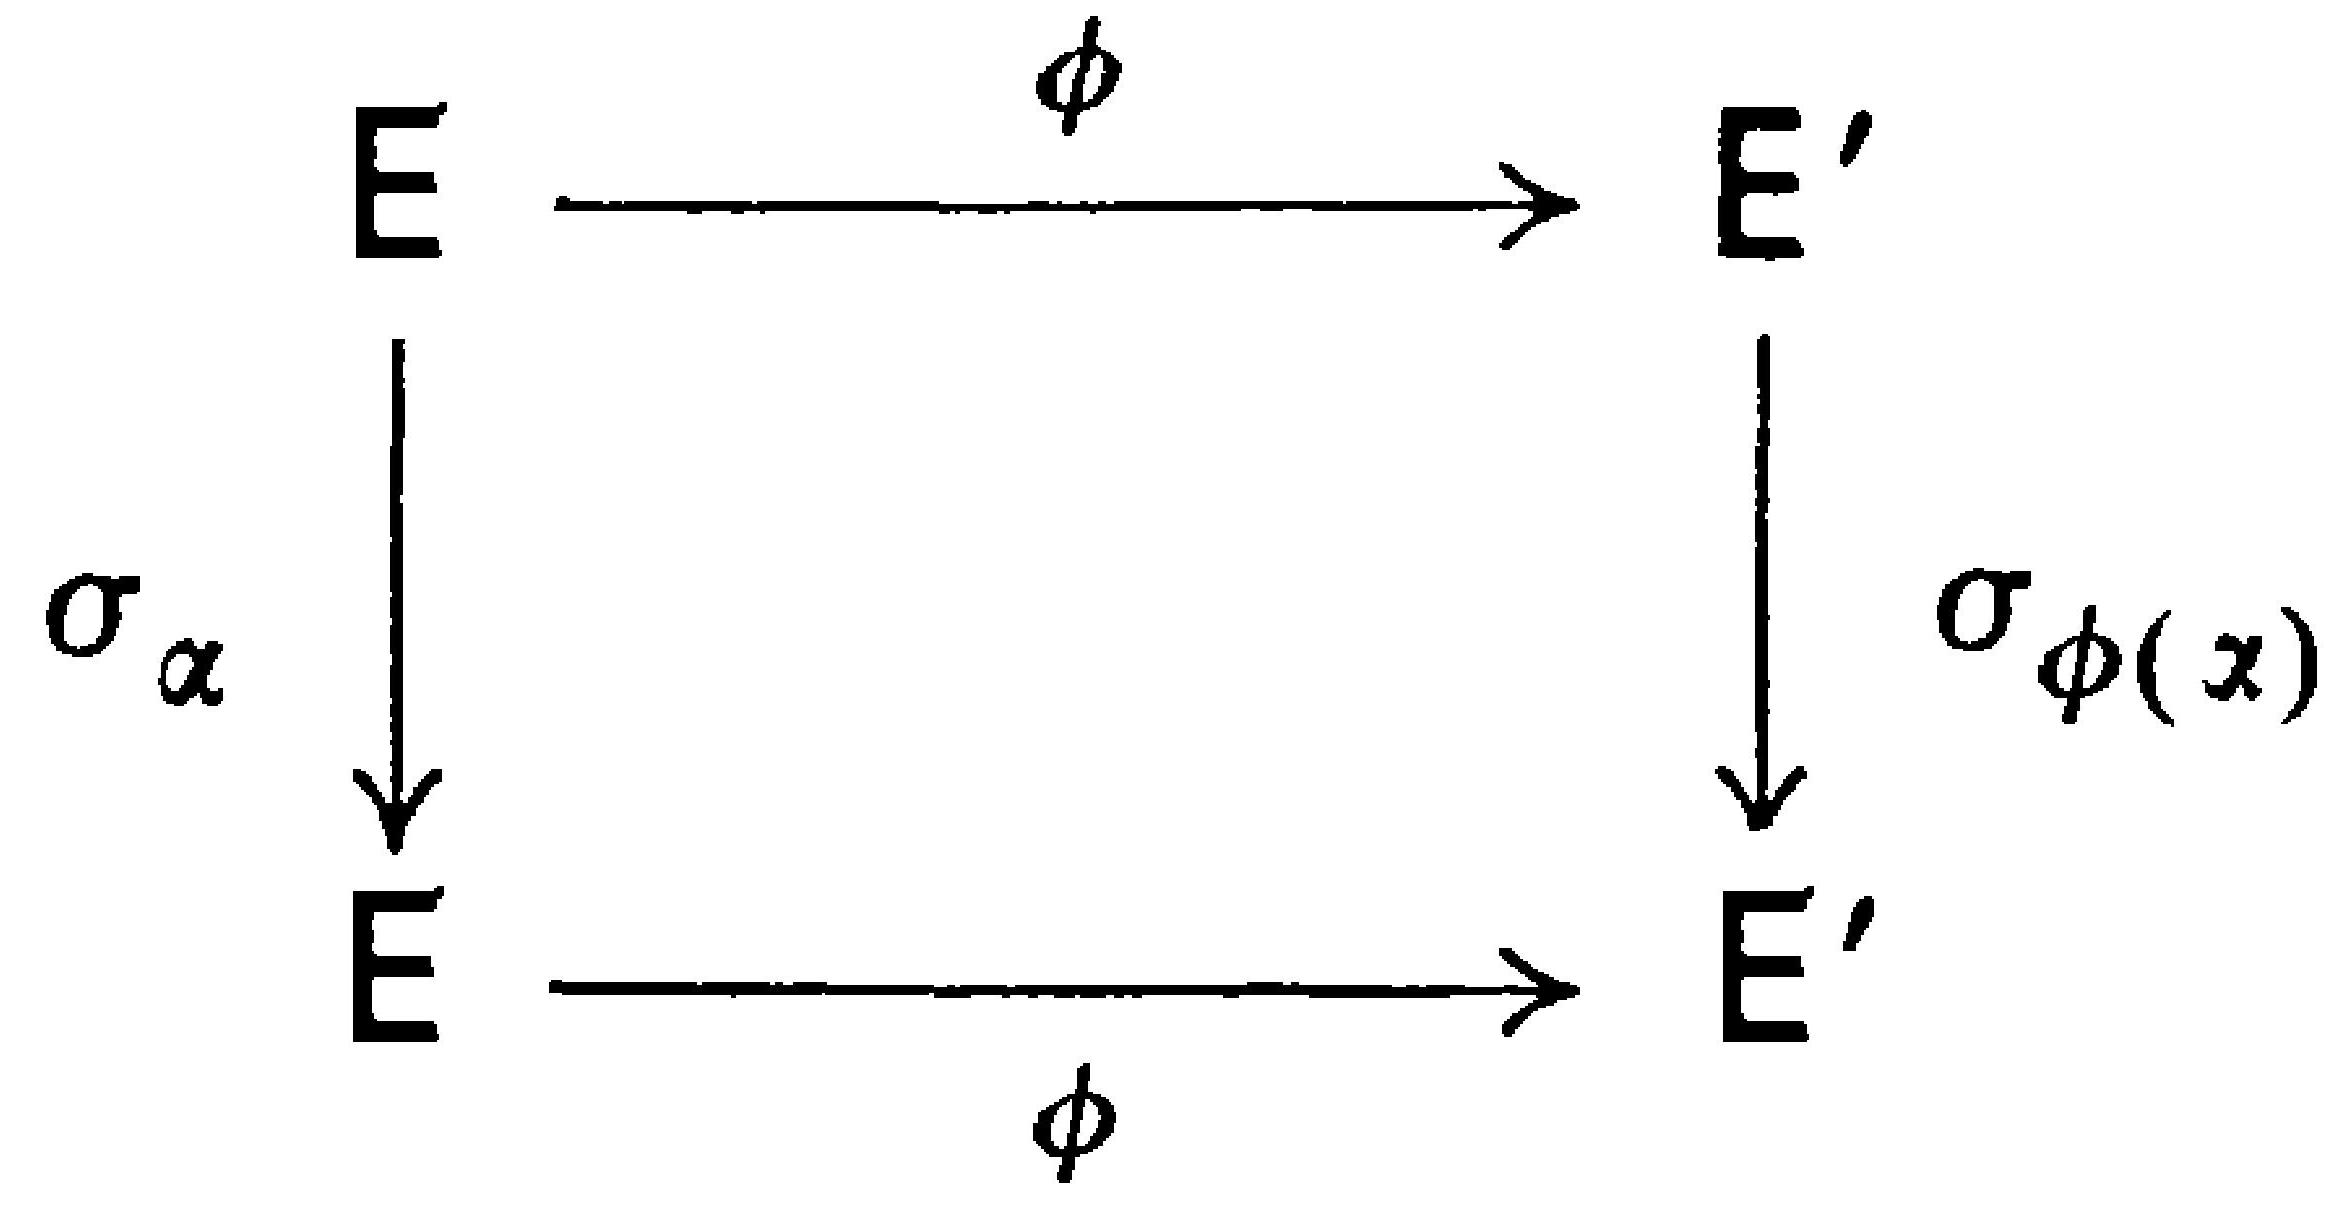
\includegraphics[max width=\textwidth, center]{2025_06_06_fac2836a92464059da43g-069}

The respective Weyl groups $\mathscr{W}, \mathscr{W}^{\prime}$ are generated by simple reflections (Theorem 10.3(d)), so it follows that the map $\sigma \mapsto \phi \circ \sigma \circ \phi^{-1}$ is an isomorphism of $\mathscr{W}$ onto $\mathscr{W}^{\prime}$, sending $\sigma_{\alpha}$ to $\sigma_{\phi(\alpha)}(\alpha \in \Delta)$. But each $\beta \in \Phi$ is conjugate under $\mathscr{W}$ to a simple root (Theorem 10.3(c)), say $\beta=\sigma(\alpha)(\alpha \in \Delta)$. This in turn forces $\phi(\beta)=\left(\phi \circ \sigma \circ \phi^{-1}\right)(\phi(\alpha)) \in \Phi^{\prime}$. It follows that $\phi$ maps $\Phi$ onto $\Phi^{\prime}$; moreover, the formula for a reflection shows that $\phi$ preserves all Cartan integers.

The proposition shows that it is possible in principle to recover $\Phi$ from a knowledge of the Cartan integers. In fact, it is not too hard to devise a practical algorithm for writing down all roots (or just all positive roots). Probably the best approach is to consider root strings (9.4). Start with the roots of height one, i.e., the simple roots. For any pair $\alpha_{i} \neq \alpha_{j}$, the integer $r$ for the $\alpha_{j}$-string through $\alpha_{i}$ is 0 (i.e., $\alpha_{i}-\alpha_{j}$ is not a root, thanks to Lemma 10.1), so the integer $q$ equals $-\left\langle\alpha_{i}, \alpha_{j}\right\rangle$. This enables us in particular to write down all roots $\alpha$ of height 2 , hence all integers $\left\langle\alpha, \alpha_{j}\right\rangle$. For each root $\alpha$ of height 2 , the integer $r$ for the $\alpha_{j}$-string through $\alpha$ can be determined easily, since $\alpha_{j}$ can be subtracted at most once (why?), and then $q$ is found, because we know $r-q=\left\langle\alpha, \alpha_{j}\right\rangle$. The corollary of Lemma 10.2A assures us that all positive roots are eventually obtained if we repeat this process enough times.

\subsection*{11.2. Coxeter graphs and Dynkin diagrams}
If $\alpha, \beta$ are distinct positive roots, then we know that $\langle\alpha, \beta\rangle\langle\beta, \alpha\rangle=0$, 1, 2, or 3 (9.4). Define the Coxeter graph of $\Phi$ to be a graph having $\ell$ vertices, the $i$ th joined to the $j$ th $(i \neq j)$ by $\left\langle\alpha_{i}, \alpha_{j}\right\rangle\left\langle\alpha_{j}, \alpha_{i}\right\rangle$ edges. Examples:\\
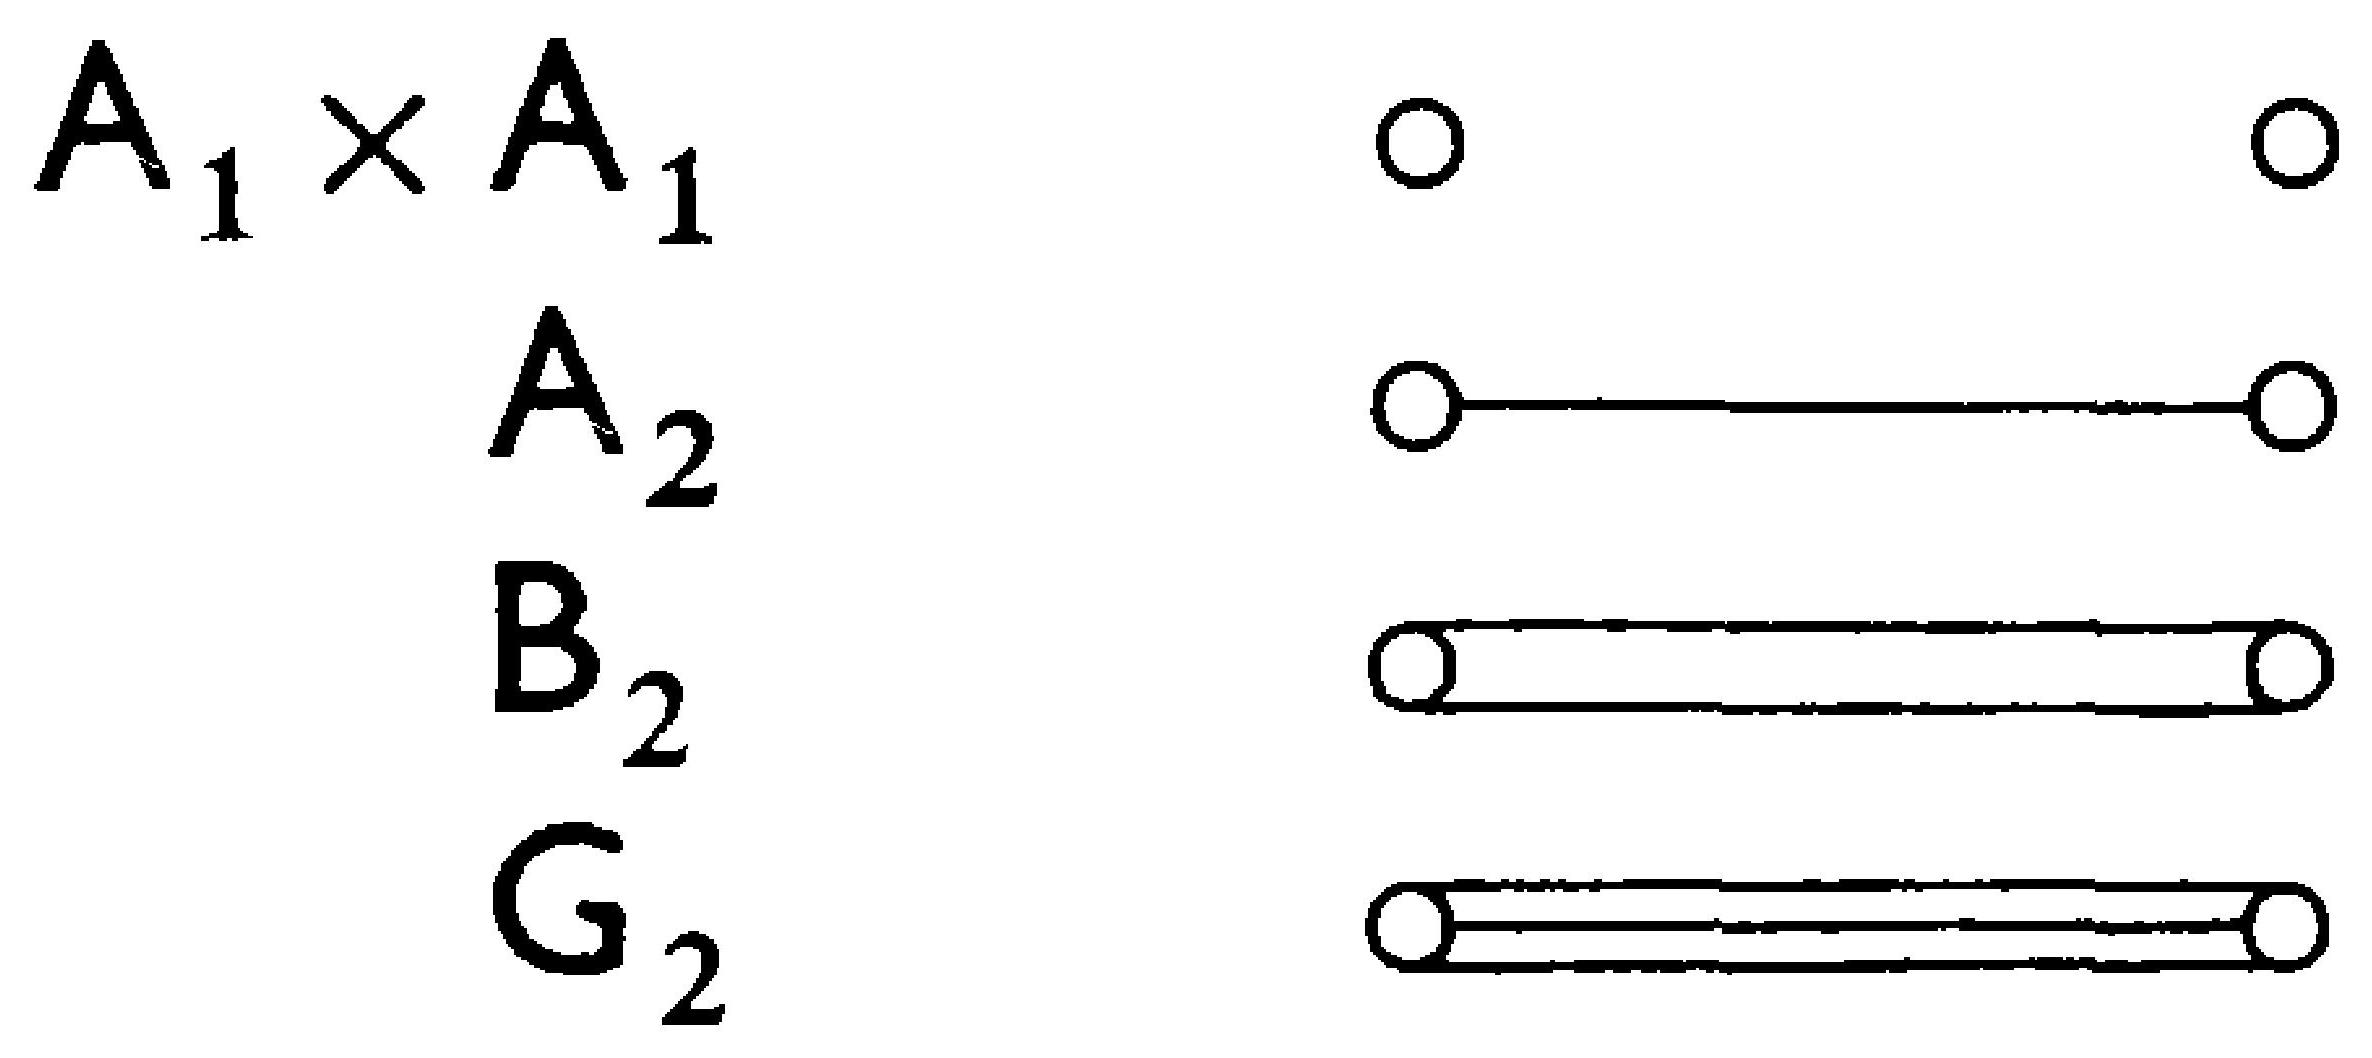
\includegraphics[max width=\textwidth, center]{2025_06_06_fac2836a92464059da43g-069(1)}

The Coxeter graph determines the numbers $\left\langle\alpha_{i}, \alpha_{j}\right\rangle$ in case all roots have equal length, since then $\left\langle\alpha_{i}, \alpha_{j}\right\rangle=\left\langle\alpha_{j}, \alpha_{i}\right\rangle$. In case more than one root length occurs (e.g., $\mathrm{B}_{2}$ or $\mathrm{G}_{2}$ ), the graph fails to tell us which of a pair of vertices should correspond to a short simple root, which to a long (in case these vertices are joined by two or three edges). (It can, however, be proved that the Coxeter graph determines the Weyl group completely, essentially\\
because it determines the orders of products of generators of $\mathscr{W}$, cf. Exercise 9.3.)

Whenever a double or triple edge occurs in the Coxeter graph of $\Phi$, we can add an arrow pointing to the shorter of the two roots. This additional information allows us to recover the Cartan integers; we call the resulting figure the Dynkin diagram of $\Phi$. (As before, this depends on the numbering of simple roots.) For example:\\
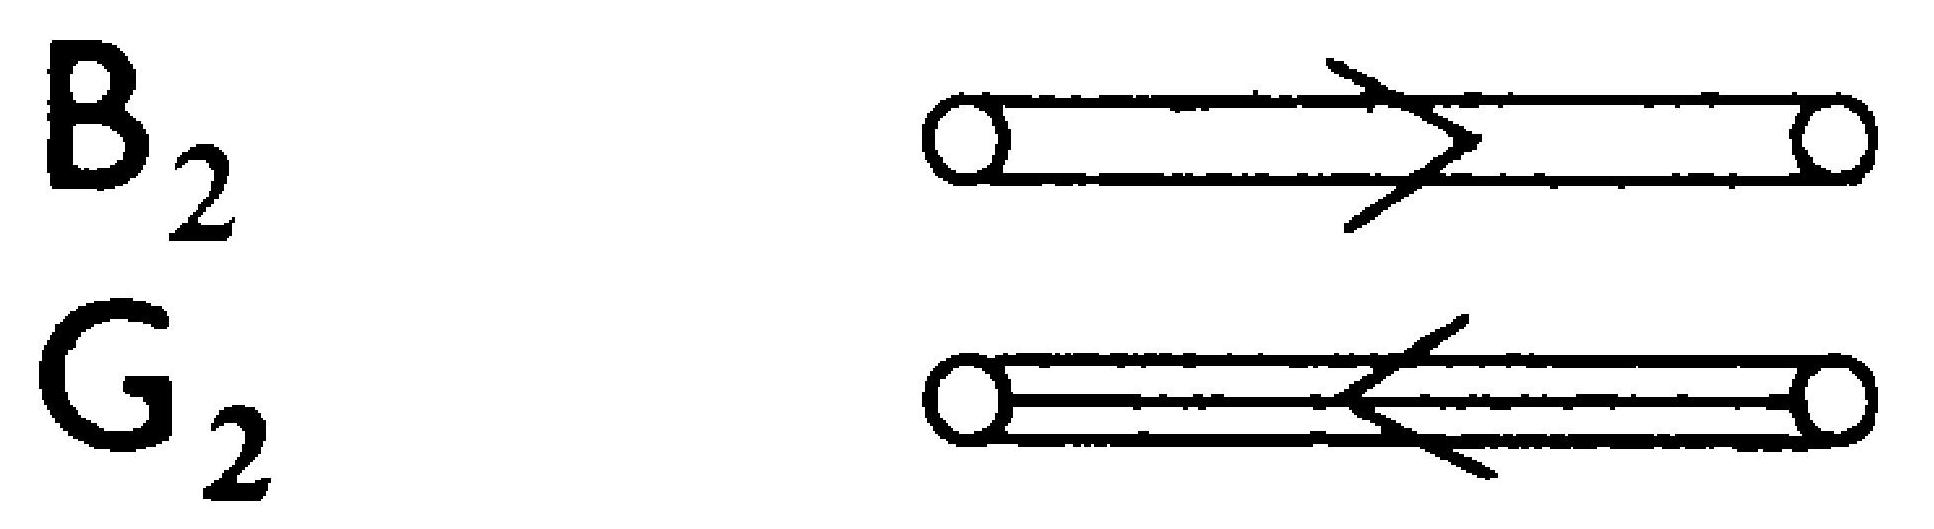
\includegraphics[max width=\textwidth, center]{2025_06_06_fac2836a92464059da43g-070}

Another example: Given the diagram O (which turns out to be associated with the root system $\mathrm{F}_{4}$ ), the reader can easily recover the Cartan matrix

$$
\left(\begin{array}{rrrr}
2 & -1 & 0 & 0 \\
-1 & 2 & -2 & 0 \\
0 & -1 & 2 & -1 \\
0 & 0 & -1 & 2
\end{array}\right)
$$

\subsection*{11.3. Irreducible components}
Recall (10.4) that $\Phi$ is irreducible if and only if $\Phi$ (or, equivalently, $\Delta$ ) cannot be partitioned into two proper, orthogonal subsets. It is clear that $\Phi$ is irreducible if and only if its Coxeter graph is connected (in the usual sense). In general, there will be a number of connected components of the Coxeter graph; let $\Delta=\Delta_{1} \cup \ldots \cup \Delta_{t}$ be the corresponding partition of $\Delta$ into mutually orthogonal subsets. If $\mathrm{E}_{i}$ is the span of $\Delta_{i}$, it is clear that $\mathrm{E}=\mathrm{E}_{1} \oplus$ $\ldots \oplus \mathrm{E}_{t}$ (orthogonal direct sum). Moreover, the Z-linear combinations of $\Delta_{i}$ which are roots (call this set $\Phi_{i}$ ) obviously form a root system in $E_{i}$, whose Weyl group is the restriction to $E_{i}$ of the subgroup of $\mathscr{W}$ generated by all $\sigma_{\alpha}\left(\alpha \in \Delta_{i}\right)$. Finally, each $\mathrm{E}_{i}$ is $\mathscr{W}$-invariant (since $\alpha \notin \Delta_{i}$ implies that $\sigma_{\alpha}$ acts trivially on $E_{i}$ ), so the (easy) argument required for Exercise 9.1 shows immediately that each root lies in one of the $E_{i}$, i.e., $\Phi=\Phi_{1} \cup \ldots \cup \Phi_{t}$.

Proposition. $\Phi$ decomposes (uniquely) as the union of irreducible root systems $\Phi_{i}$ (in subspaces $\mathrm{E}_{i}$ of E ) such that $\mathrm{E}=\mathrm{E}_{1} \oplus \ldots \oplus \mathrm{E}_{t}$ (orthogonal direct sum).

\subsection*{11.4. Classification theorem}
The discussion in (11.3) shows that it is sufficient to classify the irreducible root systems, or equivalently, the connected Dynkin diagrams (cf. Proposition 11.1).

Theorem. If $\Phi$ is an irreducible root system of rank $\ell$, its Dynkin diagram is one of the following ( $\ell$ vertices in each case):\\
\includegraphics[max width=\textwidth, center]{2025_06_06_fac2836a92464059da43g-071}

The restrictions on $\ell$ for types $A_{\ell}-D_{\ell}$ are imposed in order to avoid duplication. Relative to the indicated numbering of simple roots, the corresponding Cartan matrices are given in Table 1. Inspection of the diagrams listed above reveals that in all cases except $\mathrm{B}_{\ell}, \mathrm{C}_{\ell}$, the Dynkin diagram can be deduced from the Coxeter graph. However, $\mathrm{B}_{\ell}$ and $\mathrm{C}_{\ell}$ both come from a single Coxeter graph, and differ in the relative numbers of short and long simple roots. (These root systems are actually dual to each other, cf. Exercise 5.)

Proof of Theorem. The idea of the proof is to classify first the possible Coxeter graphs (ignoring relative lengths of roots), then see what Dynkin diagrams result. Therefore, we shall merely apply some elementary euclidean geometry to finite sets of vectors whose pairwise angles are those prescribed by the Coxeter graph. Since we are ignoring lengths, it is easier to work for the time being with sets of unit vectors. For maximum flexibility, we make

Table 1. Cartan matrices

\begin{center}
\begin{tabular}{|l|l|l|l|l|l|l|l|l|l|}
\hline
\multicolumn{10}{|c|}{$A_{\ell}:\left(\begin{array}{rrrrrlllll}2 & -1 & 0 & & & . & . & . & & 0 \\ -1 & 2 & -1 & 0 & & . & . & . & & 0 \\ 0 & -1 & 2 & -1 & 0 & . & . & . & & 0 \\ . & . & . & . & . & . & . & . & . & . \\ 0 & 0 & 0 & 0 & & . & . & . & -1 & 2\end{array}\right)$} \\
\hline
\multicolumn{10}{|c|}{$\mathrm{B}_{\ell}:\left(\begin{array}{rrrrlllrr}2 & -1 & 0 & & . & . & . & & 0 \\ -1 & 2 & -1 & 0 & . & . & . & & 0 \\ . & . & . & . & . & . & . & . & . \\ 0 & 0 & 0 & & . & . & . & -1 & 2 \\ 0 & 0 & 0 & & . & . & . & 0 & -1 \\ 2\end{array}\right)$} \\
\hline
\multicolumn{10}{|c|}{test} \\
\hline
\multirow{2}{*}{} & \multicolumn{9}{|c|}{\begin{tabular}{l}
$\left(\begin{array}{rrrlcccrrr}2 & -1 & 0 & & . & . & . & & 0 \\ -1 & 2 & -1 & & . & . & . & & 0 \\ . & . & . & . & . & . & . & . & . & . \\ 0 & 0 & & . & . & -1 & 2 & -1 & 0 & 0 \\ 0 & 0 & & . & . & & -1 & 2 & -1 & -1 \\ 0 & 0 & & . & . & & 0 & -1 & 2 & 0 \\ 0 & 0 & & . & . & & 0 & -1 & 0 & 2\end{array}\right)$ \\
$\left.\begin{array}{l}0 \\ 1 \\ 2\end{array}\right)$ \\
$\left(\begin{array}{rrrlccccrr}2 & -1 & 0 & & . & . & . & & 0 \\ -1 & 2 & -1 & & . & . & . & & 0 \\ . & . & . & . & . & . & . & . & . & . \\ 0 & 0 & & . & . & -1 & 2 & -1 & 0 & 0 \\ 0 & 0 & & . & . & & -1 & 2 & -1 & -1 \\ 0 & 0 & & . & . & & 0 & -1 & 2 & 0 \\ 0 & 0 & & . & . & & 0 & -1 & 0 & 2\end{array}\right)$ \\
\end{tabular}} \\
\hline
\multicolumn{10}{|l|}{$\mathrm{E}_{6}:\left(\begin{array}{rrrrrr}2 & 0 & -1 & 0 & 0 & 0 \\ 0 & 2 & 0 & -1 & 0 & 0 \\ -1 & 0 & 2 & -1 & 0 & 0 \\ 0 & -1 & -1 & 2 & -1 & 0 \\ 0 & 0 & 0 & -1 & 2 & -1 \\ 0 & 0 & 0 & 0 & -1 & 2\end{array}\right)$} \\
\hline
\multicolumn{10}{|l|}{\begin{tabular}{l}
$\left(\begin{array}{cccccc}2 & 0 & -1 & 0 & 0 & 0\end{array}\right.$ \\
$\mathrm{E}_{7}:\left(\begin{array}{rrrrrrr}2 & 0 & -1 & 0 & 0 & 0 & 0 \\ 0 & 2 & 0 & -1 & 0 & 0 & 0 \\ -1 & 0 & 2 & -1 & 0 & 0 & 0 \\ 0 & -1 & -1 & 2 & -1 & 0 & 0 \\ 0 & 0 & 0 & -1 & 2 & -1 & 0 \\ 0 & 0 & 0 & 0 & -1 & 2 & -1 \\ 0 & 0 & 0 & 0 & 0 & -1 & 2\end{array}\right)$ \\
\end{tabular}} \\
\hline
\multicolumn{10}{|l|}{$\mathrm{E}_{8}:\left(\begin{array}{rrrrrrrr}2 & 0 & -1 & 0 & 0 & 0 & 0 & 0 \\ 0 & 2 & 0 & -1 & 0 & 0 & 0 & 0 \\ -1 & 0 & 2 & -1 & 0 & 0 & 0 & 0 \\ 0 & -1 & -1 & 2 & -1 & 0 & 0 & 0 \\ 0 & 0 & 0 & -1 & 2 & -1 & 0 & 0 \\ 0 & 0 & 0 & 0 & -1 & 2 & -1 & 0 \\ 0 & 0 & 0 & 0 & 0 & -1 & 2 & -1 \\ 0 & 0 & 0 & 0 & 0 & 0 & -1 & 2\end{array}\right)$} \\
\hline
\multicolumn{10}{|l|}{$\mathrm{F}_{4}:\left(\begin{array}{rrrr}2 & -1 & 0 & 0 \\ -1 & 2 & -2 & 0 \\ 0 & -1 & 2 & -1 \\ 0 & 0 & -1 & 2\end{array}\right) \quad \mathrm{G}_{2}:\left(\begin{array}{rr}2 & -1 \\ -3 & 2\end{array}\right)$} \\
\hline
\end{tabular}
\end{center}

only the following assumptions: E is a euclidean space (of arbitrary dimension), $\mathfrak{A}=\left\{\varepsilon_{1}, \ldots, \varepsilon_{n}\right\}$ is a set of $n$ linearly independent unit vectors which satisfy $\left(\varepsilon_{i}, \varepsilon_{j}\right) \leq 0(i \neq j)$ and $4\left(\varepsilon_{i}, \varepsilon_{j}\right)^{2}=0,1,2$, or $3(i \neq j)$. Such a set of vectors is called (for brevity) admissible. (Example: Elements of a base for a root system, each divided by its length.) We attach a graph $\Gamma$ to the set $\mathfrak{A}$ just as we did above to the simple roots in a root system, with vertices $i$ and $j$ $(i \neq j)$ joined by $4\left(\varepsilon_{i}, \varepsilon_{j}\right)^{2}$ edges. Now our task is to determine all the connected graphs associated with admissible sets of vectors (these include all connected Coxeter graphs). This we do in steps, the first of which is obvious. ( $\Gamma$ is not assumed to be connected until later on.)\\
(1) If some of the $\varepsilon_{i}$ are discarded, the remaining ones still form an admissible set, whose graph is obtained from $\Gamma$ by omitting the corresponding vertices and all incident edges.\\
(2) The number of pairs of vertices in $\Gamma$ connected by at least one edge is strictly less than $n$. Set $\varepsilon=\sum_{i=1}^{n} \varepsilon_{i}$. Since the $\varepsilon_{i}$ are linearly independent, $\varepsilon \neq 0$. So $0<(\varepsilon, \varepsilon)=n+2 \sum_{i<j}\left(\varepsilon_{i}, \varepsilon_{j}\right)$. Let $i, j$ be a pair of (distinct) indices for which $\left(\varepsilon_{i}, \varepsilon_{j}\right) \neq 0$ (i.e., let vertices $i$ and $j$ be joined). Then $4\left(\varepsilon_{i}, \varepsilon_{j}\right)^{2}=1,2$, or 3 , so in particular $2\left(\varepsilon_{i}, \varepsilon_{j}\right) \leq-1$. In view of the above inequality, the number of such pairs cannot exceed $n-1$.\\
(3) $\Gamma$ contains no cycles. A cycle would be the graph $\Gamma^{\prime}$ of an admissible subset $\mathfrak{A}^{\prime}$ of $\mathfrak{A}$ (cf. (1)), and then $\Gamma^{\prime}$ would violate (2), with $n$ replaced by Card $\mathfrak{A}^{\prime}$.\\
(4) No more than three edges can originate at a given vertex of $\Gamma$. Say $\varepsilon \in \mathfrak{A}$, and $\eta_{1}, \ldots, \eta_{k}$ are the vectors in $\mathfrak{A}$ connected to $\varepsilon$ (by 1,2 , or 3 edges each), i.e., $\left(\varepsilon, \eta_{i}\right)<0$ with $\varepsilon, \eta_{1}, \ldots, \eta_{k}$ all distinct. In view of (3), no two $\eta$ 's can be connected, so $\left(\eta_{i}, \eta_{j}\right)=0$ for $i \neq j$. Because $\mathfrak{A}$ is linearly independent, some unit vector $\eta_{0}$ in the span of $\varepsilon, \eta_{1}, \ldots, \eta_{k}$ is orthogonal to $\eta_{1}, \ldots, \eta_{k}$; clearly $\left(\varepsilon, \eta_{0}\right) \neq 0$ for such $\eta_{0}$. Now $\varepsilon=\sum_{i=0}^{k}\left(\varepsilon, \eta_{i}\right) \eta_{i}$, so $1=(\varepsilon, \varepsilon)=\sum_{i=0}^{k}\left(\varepsilon, \eta_{i}\right)^{2}$. This forces $\sum_{i=1}^{k}\left(\varepsilon, \eta_{i}\right)^{2}<1$, or $\sum_{i=1}^{k} 4\left(\varepsilon, \eta_{i}\right)^{2}<4$. But $4\left(\varepsilon, \eta_{i}\right)^{2}$ is the number of edges joining $\varepsilon$ to $\eta_{i}$ in $\Gamma$.\\
(5) The only connected graph $\Gamma$ of an admissible set $\mathfrak{A}$ which can contain a triple edge is $\Longrightarrow$ (the Coxeter graph $\mathrm{G}_{2}$ ). This follows at once from (4).\\
(6) Let $\left\{\varepsilon_{1}, \ldots, \varepsilon_{k}\right\} \subset \mathfrak{A}$ have subgraph $\multimap-\cdots \cdot$ (a simple chain in $\Gamma$. If $\mathfrak{A}^{\prime}=\left(\mathfrak{A}-\left\{\varepsilon_{1}, \ldots, \varepsilon_{k}\right\}\right) \cup\{\varepsilon\}, \varepsilon=\sum_{i=1}^{k} \varepsilon_{i}$, then $\mathfrak{A}^{\prime}$ is admissible. (The graph of $\mathfrak{A}^{\prime}$ is obtained from $\Gamma$ by shrinking the simple chain to a point.) Linear independence of $\mathfrak{A}^{\prime}$ is obvious. By hypothesis, $2\left(\varepsilon_{i}, \varepsilon_{i+1}\right)=$ $-1(1 \leq i \leq k-1)$, so $(\varepsilon, \varepsilon)=k+2 \sum_{i<j}\left(\varepsilon_{i}, \varepsilon_{j}\right)=k-(k-1)=1$. So $\varepsilon$ is a unit vector. Any $\eta \in \mathfrak{A}-\left\{\varepsilon_{1}, \ldots, \varepsilon_{k}\right\}$ can be connected to at most one of $\varepsilon_{1}, \ldots, \varepsilon_{k}$ (by (3)), so ( $\eta, \varepsilon$ ) = 0 or else ( $\eta, \varepsilon$ ) = ( $\eta, \varepsilon_{i}$ ) for $1 \leq i \leq k$. In either case, $4(\eta, \varepsilon)^{2}=0,1,2$, or 3 .\\
(7) $\Gamma$ contains no subgraph of the form:\\
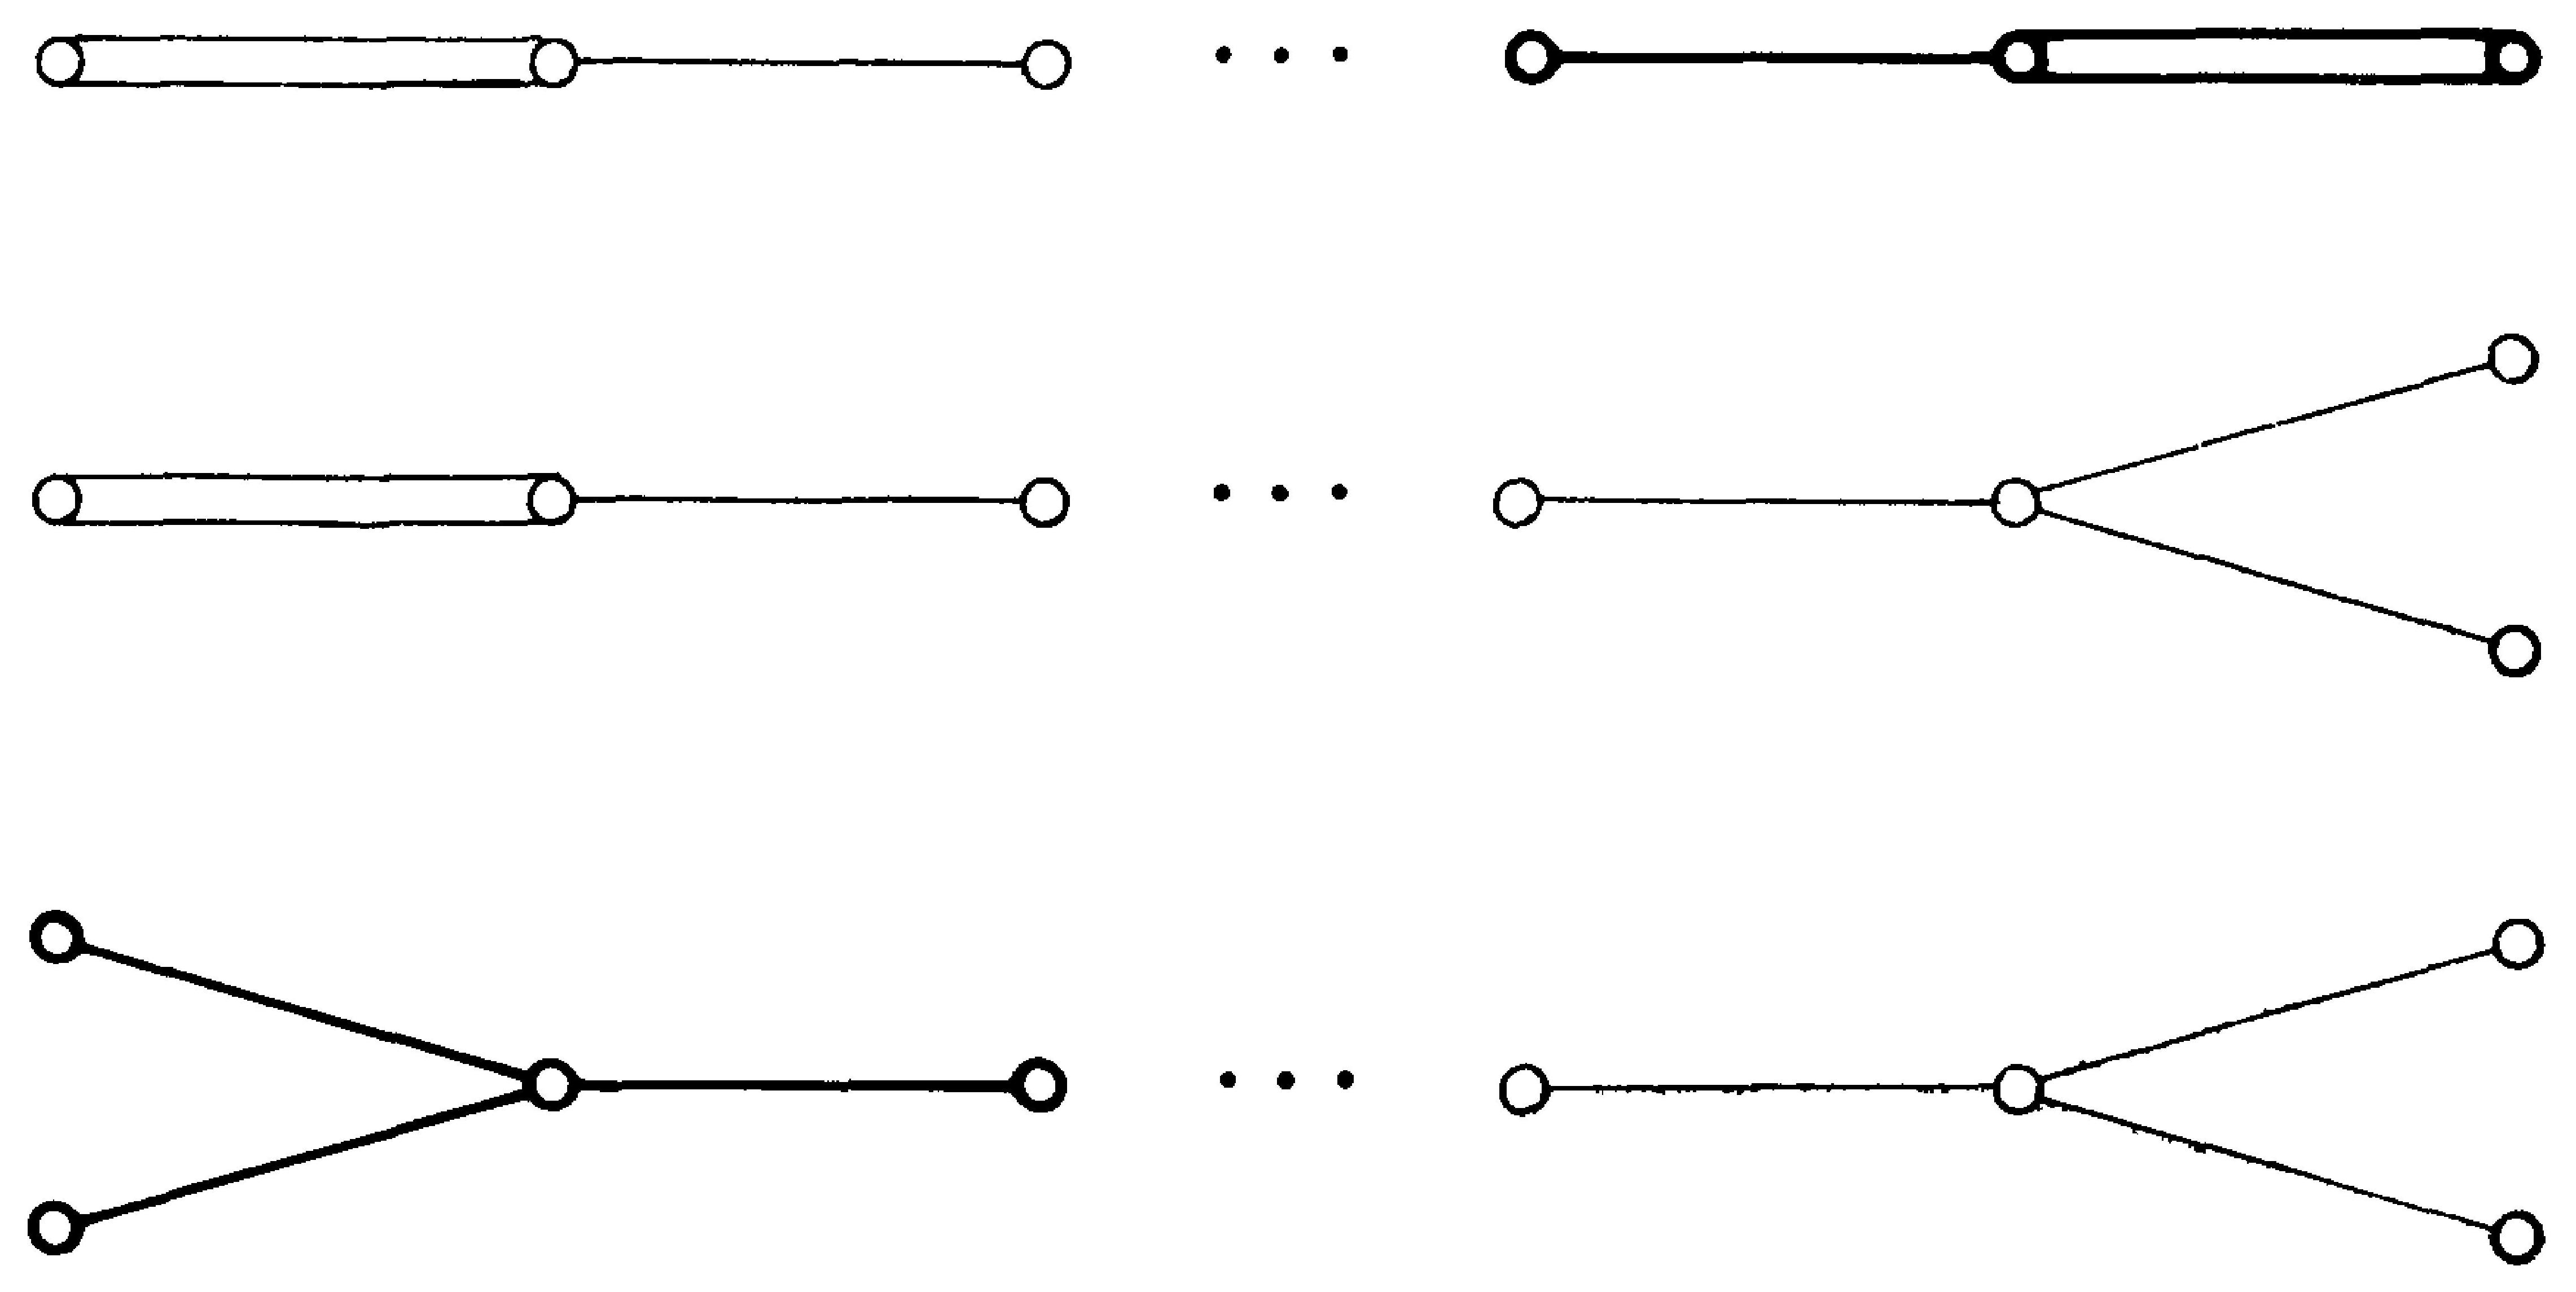
\includegraphics[max width=\textwidth, center]{2025_06_06_fac2836a92464059da43g-074(1)}

Suppose one of these graphs occurred in $\Gamma$; by (1) it would be the graph of an admissible set. But (6) allows us to replace the simple chain in each case by a single vertex, yielding (respectively) the following graphs which violate (4):\\
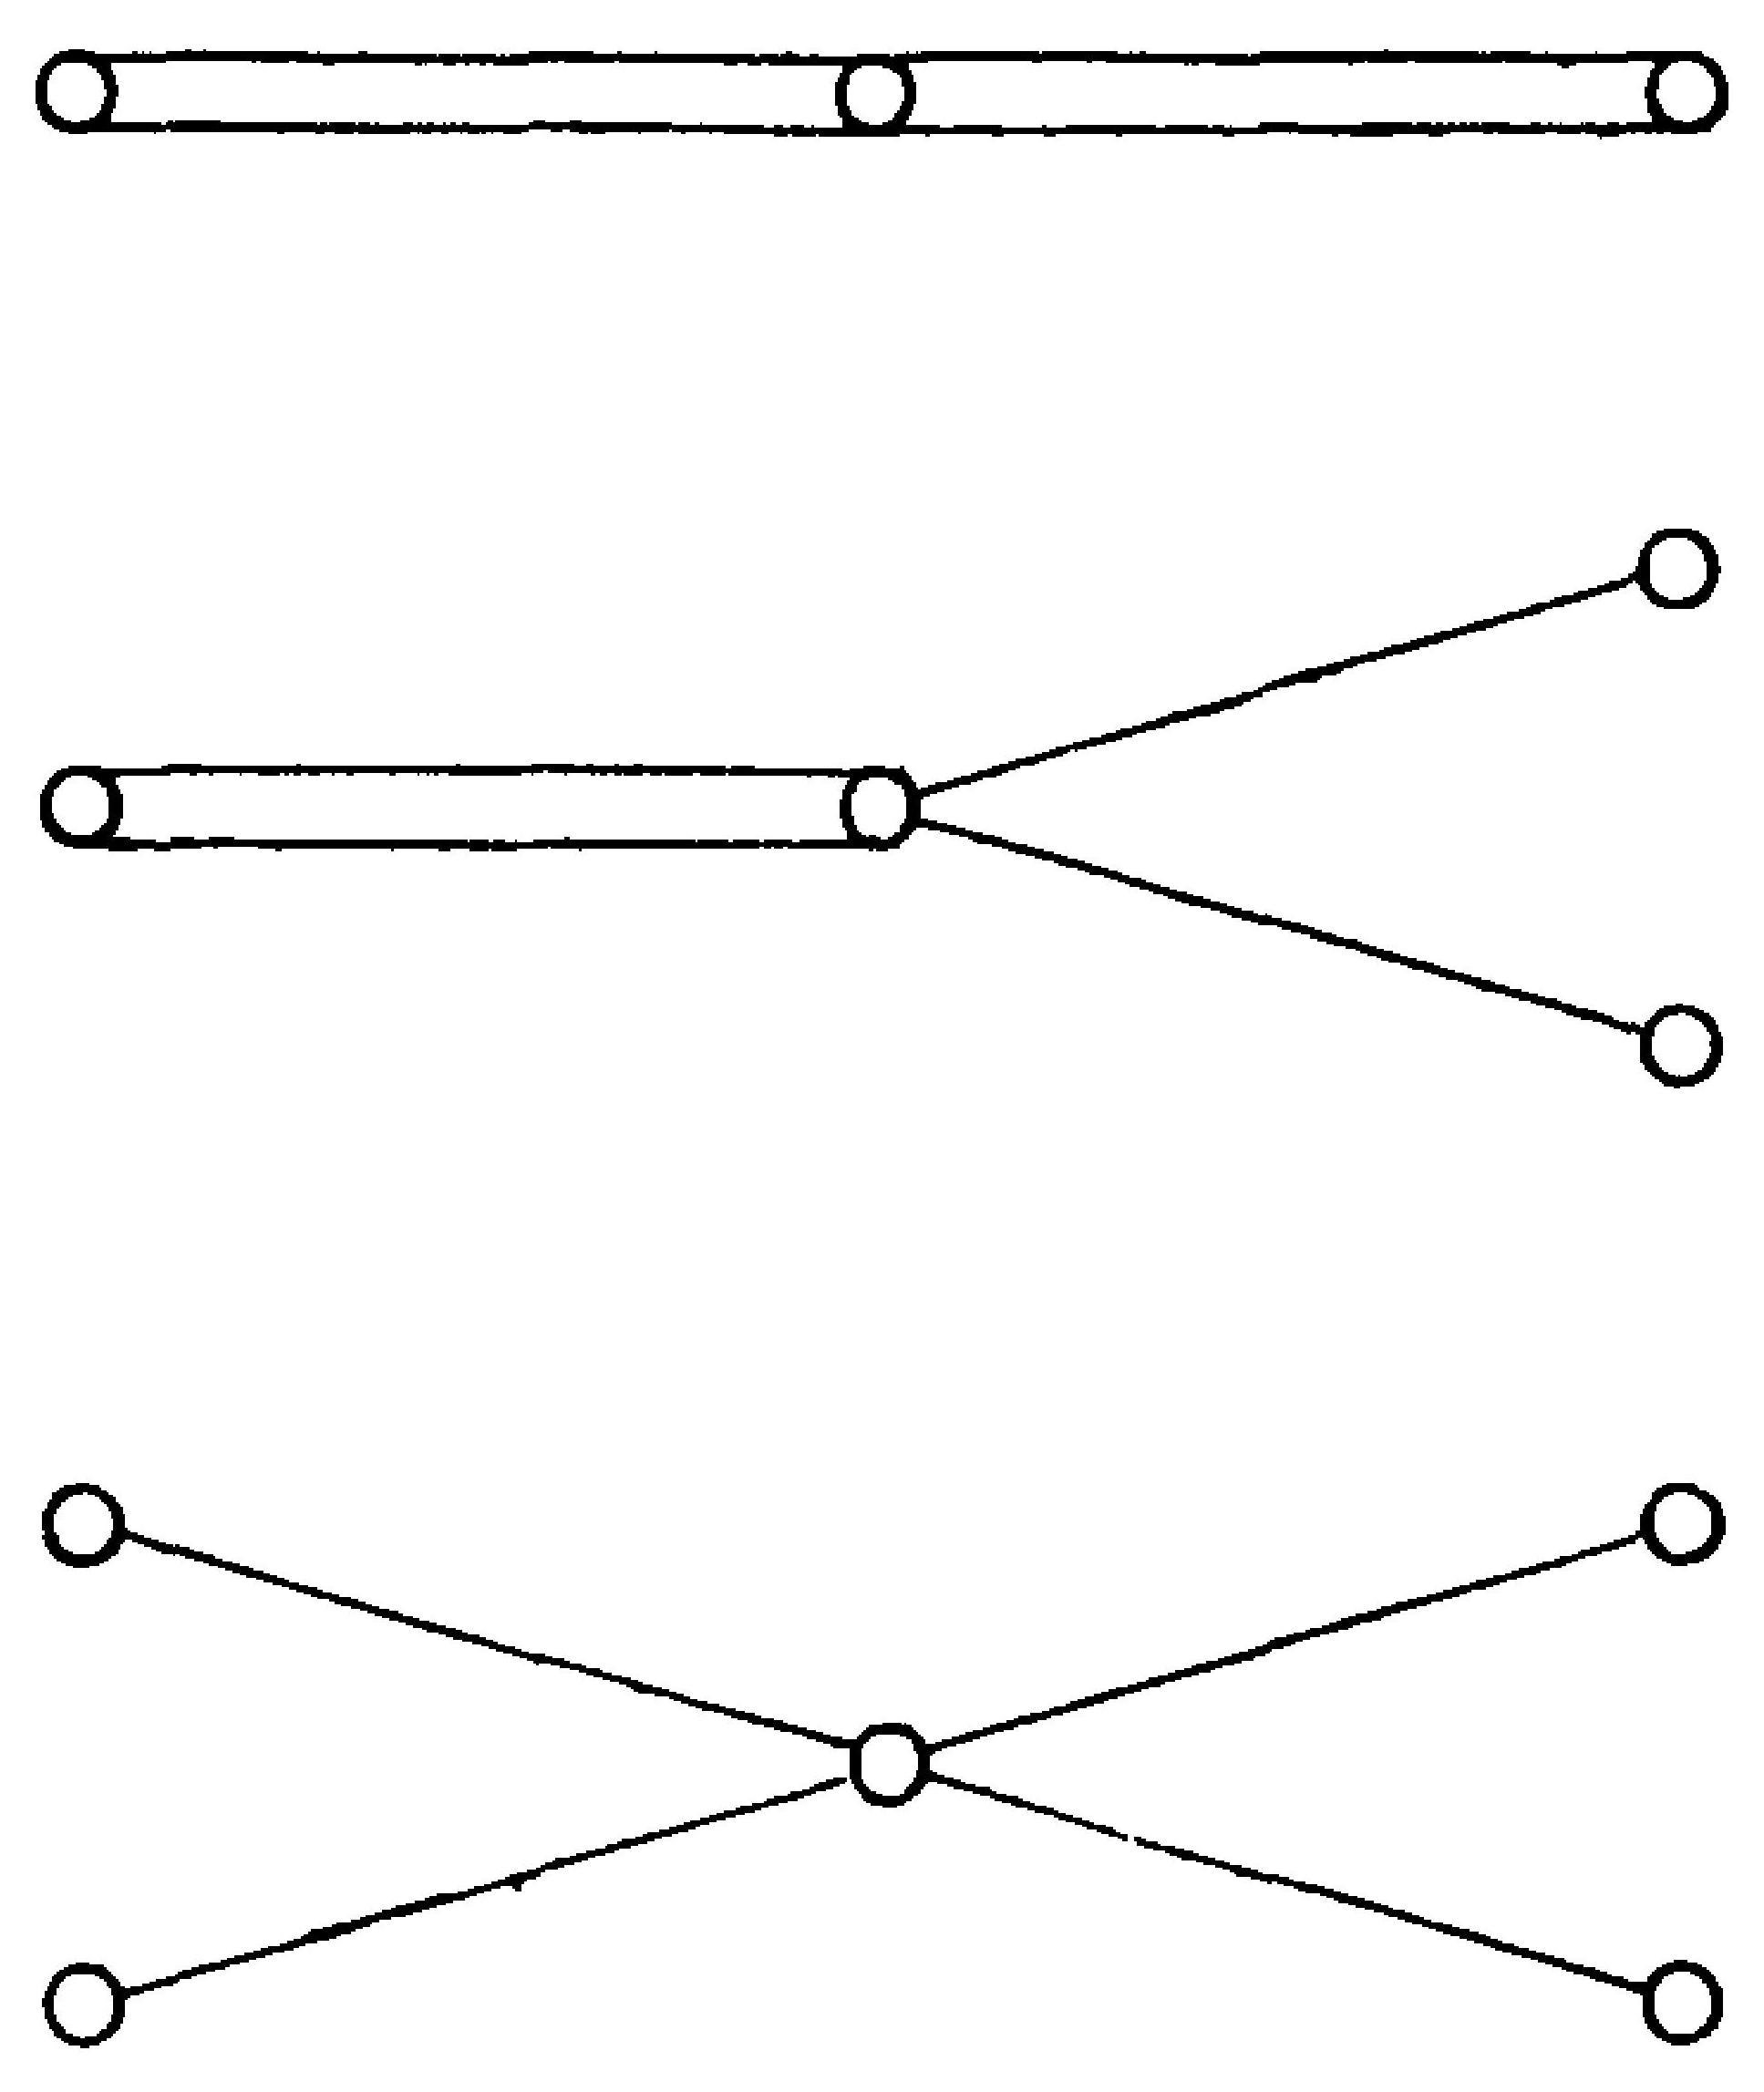
\includegraphics[max width=\textwidth, center]{2025_06_06_fac2836a92464059da43g-074}\\
(8) Any connected graph $\Gamma$ of an admissible set has one of the following forms:\\
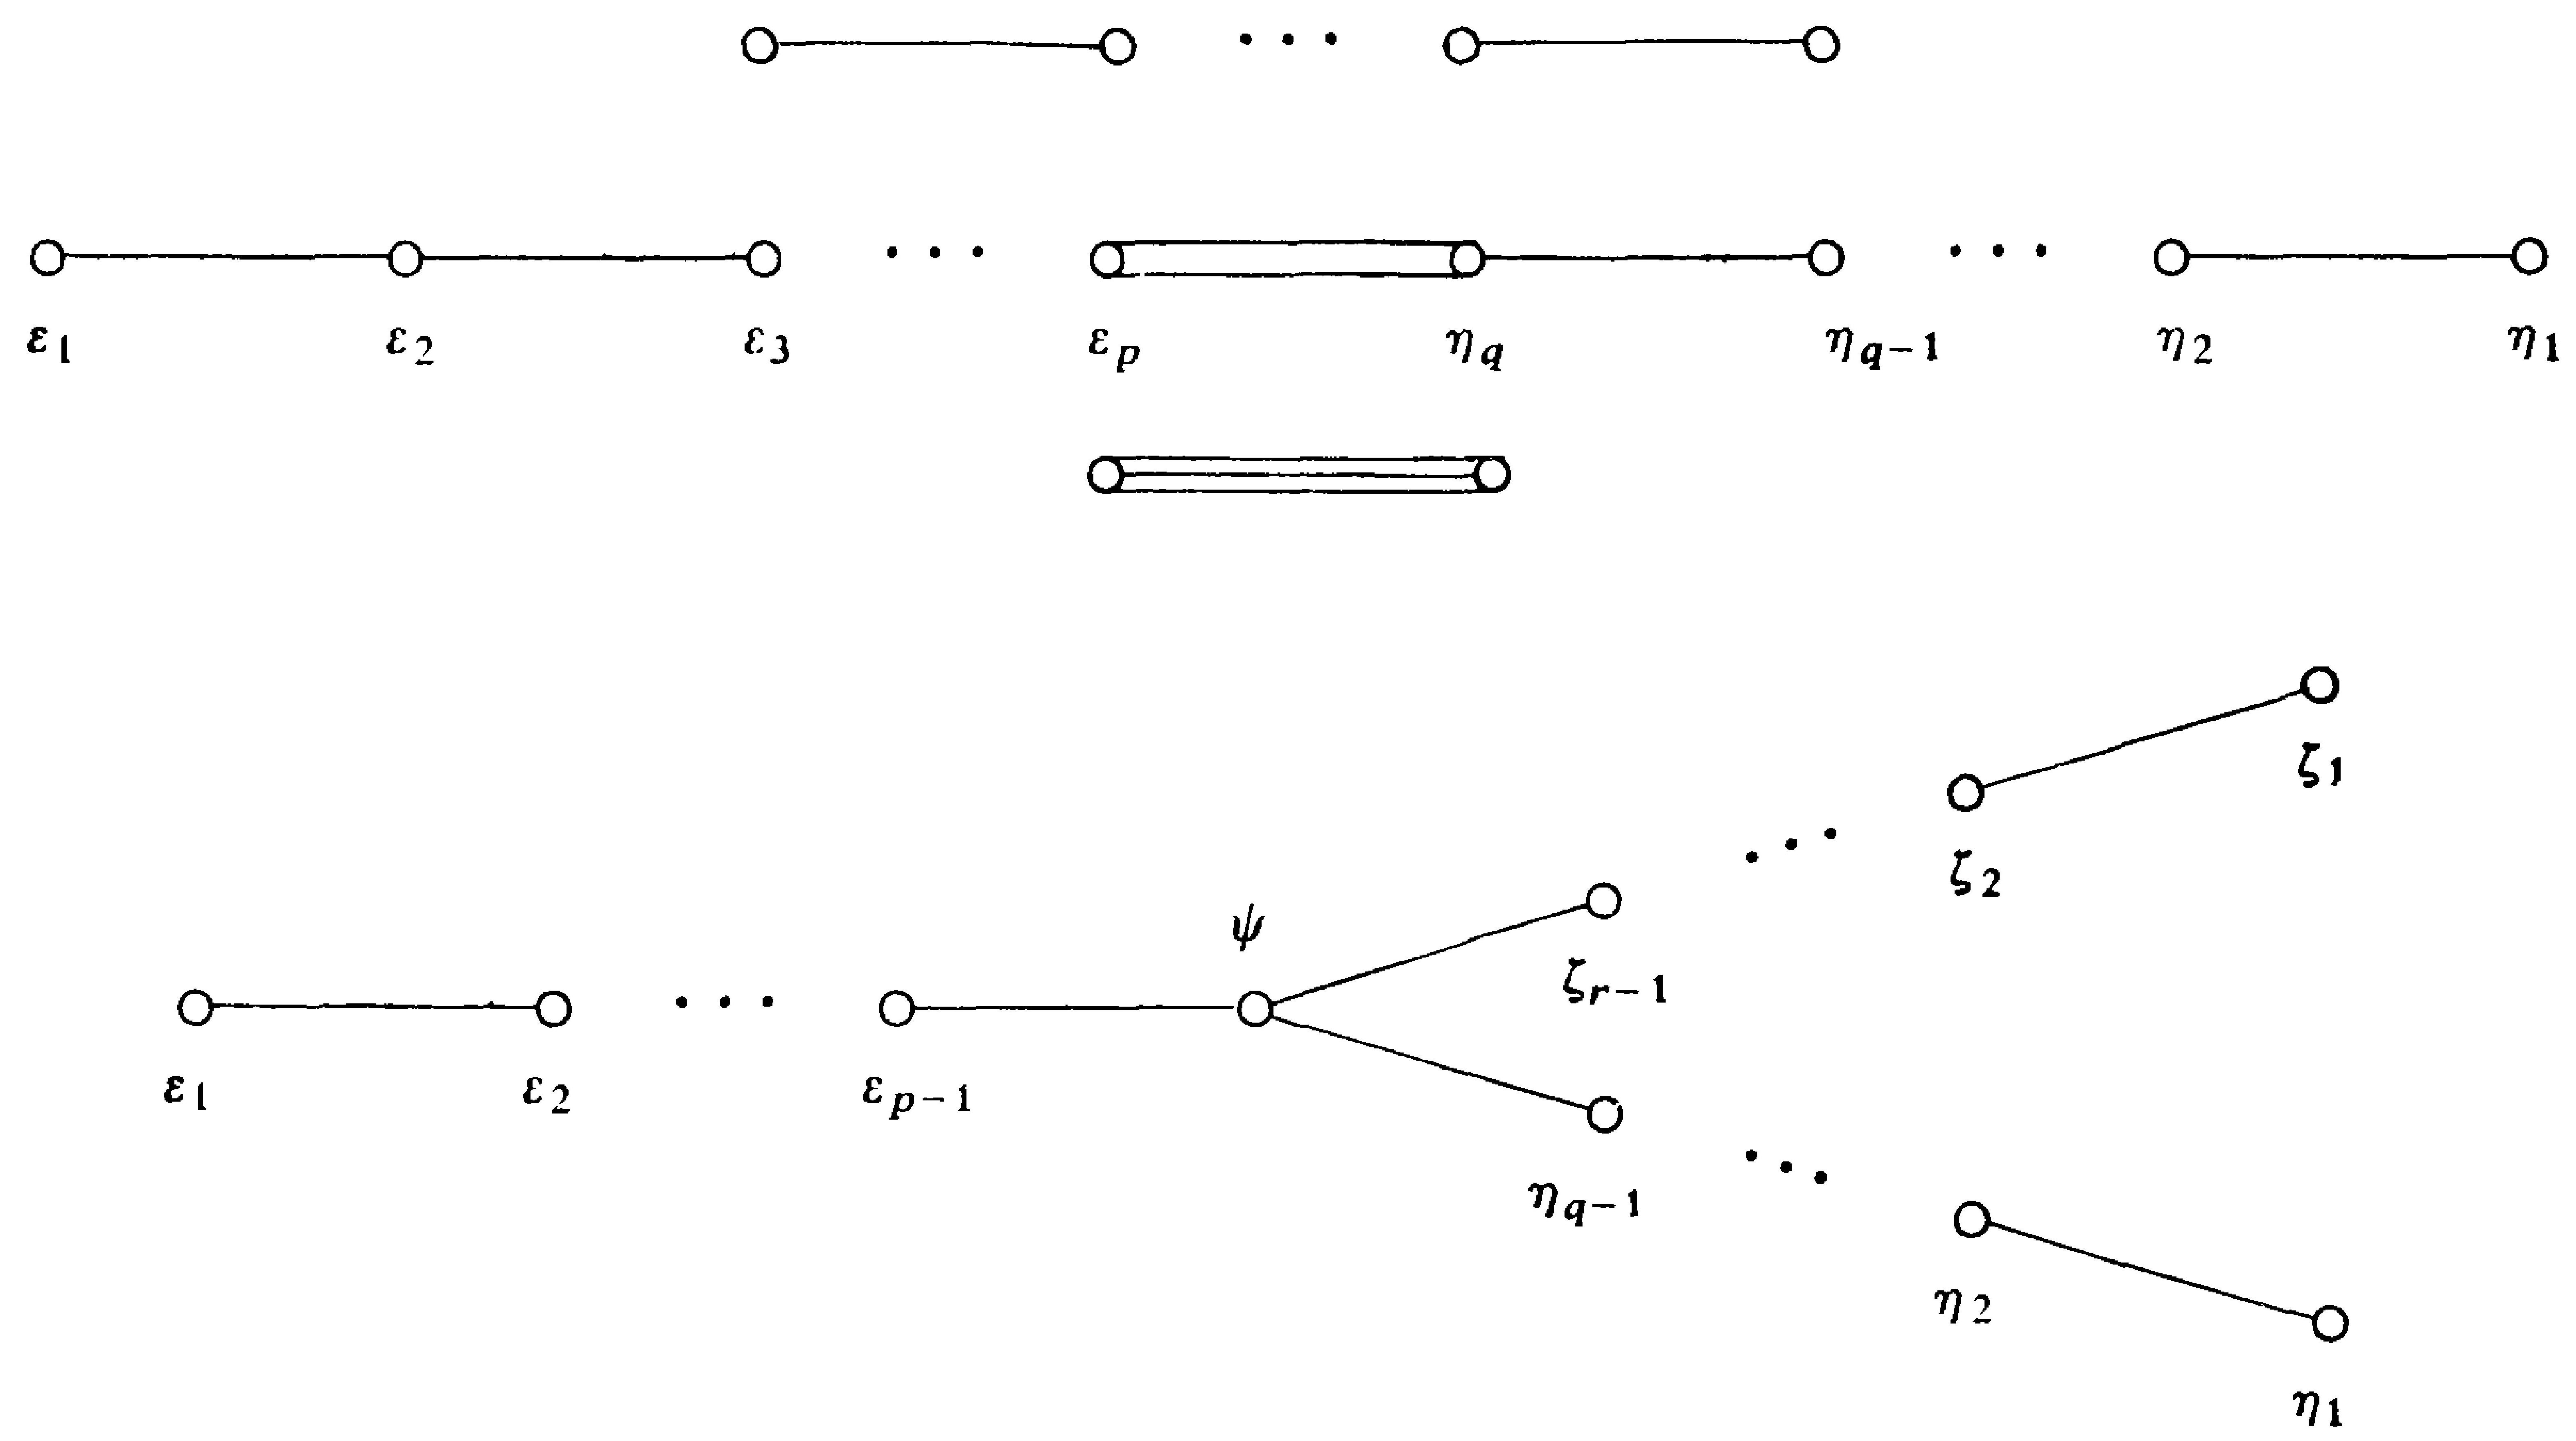
\includegraphics[max width=\textwidth, center]{2025_06_06_fac2836a92464059da43g-074(2)}

Indeed, only\\
contains a triple edge, by (5). A connected graph containing more than one double edge would contain a subgraph\\
which (7) forbids, so at most one double edge occurs. Moreover, if $\Gamma$ has a double edge, it cannot also have a "node" (branch point)\\
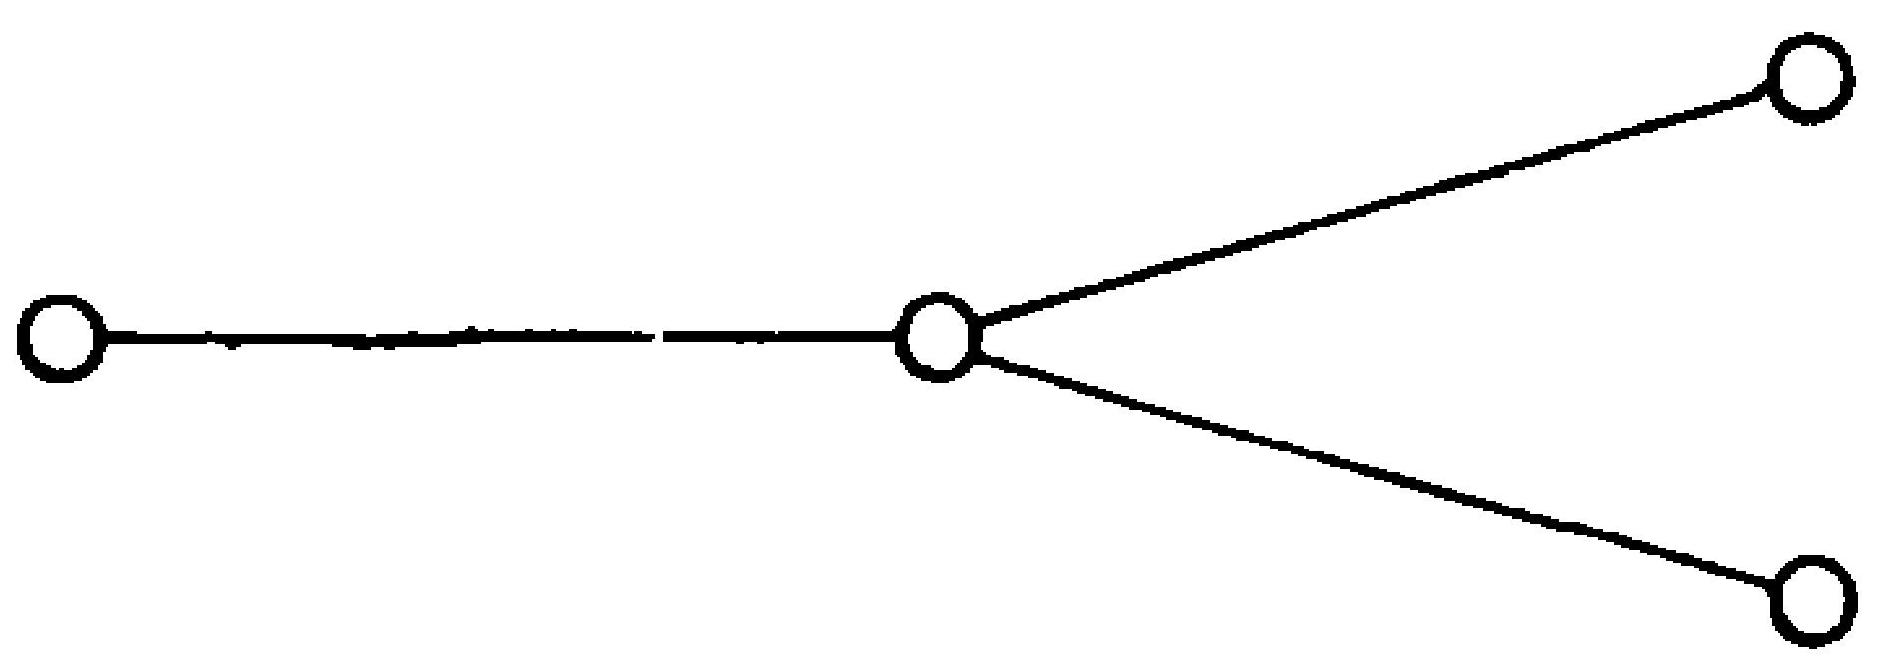
\includegraphics[max width=\textwidth, center]{2025_06_06_fac2836a92464059da43g-075}\\
(again by (7)), so the second graph pictured is the only possibility (cycles being forbidden by (3)). Finally, let $\Gamma$ have only single edges; if $\Gamma$ has no node, it must be a simple chain (again because no cycles are allowed). It cannot contain more than one node (7), so the fourth graph is the only remaining possibility.\\
(9) The only connected $\Gamma$ of the second type in (8) is the Coxeter graph $\mathrm{F}_{4}$\\
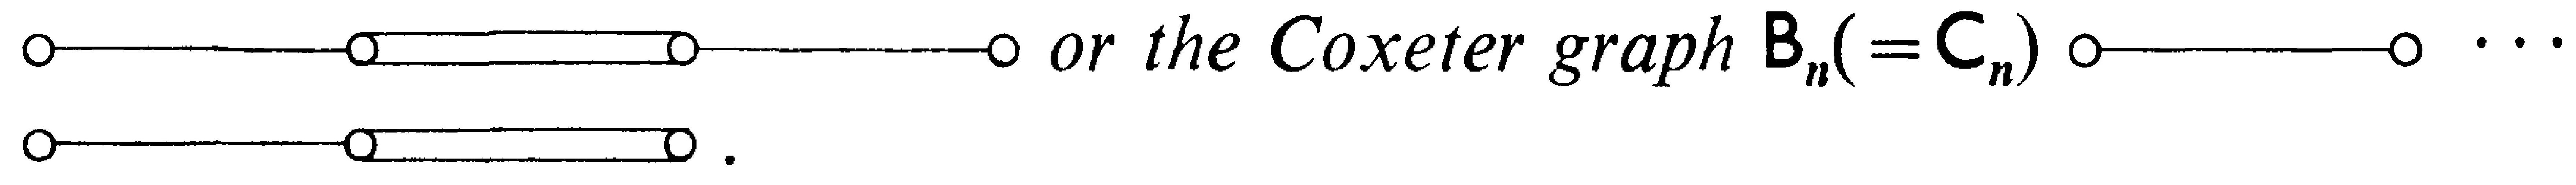
\includegraphics[max width=\textwidth, center]{2025_06_06_fac2836a92464059da43g-075(1)}

Set $\varepsilon=\sum_{i=1}^{p} i \varepsilon_{i}, \eta=\sum_{i=1}^{q} i \eta_{i}$. By hypothesis, $2\left(\varepsilon_{i}, \varepsilon_{i+1}\right)=-1=2\left(\eta_{i}, \eta_{i+1}\right)$, and other pairs are orthogonal, so $(\varepsilon, \varepsilon)=\sum_{i=1}^{p} i^{2}-\sum_{i=1}^{p-1} i(i+1)=p(p+1) / 2,(\eta, \eta)$ $=q(q+1) / 2$. Since $4\left(\varepsilon_{p}, \eta_{q}\right)^{2}=2$, we also have $(\varepsilon, \eta)^{2}=p^{2} q^{2}\left(\varepsilon_{p}, \eta_{q}\right)^{2}=$ $p^{2} q^{2} / 2$. The Schwartz inequality implies (since $\varepsilon, \eta$ are obviously independent) that $(\varepsilon, \eta)^{2}<(\varepsilon, \varepsilon)(\eta, \eta)$, or $p^{2} q^{2} / 2<p(p+1) q(q+1) / 4$, whence $(p-1)(q-1)$ $<2$. The possibilities are: $p=q=2$ (whence $\mathrm{F}_{4}$ ) or $p=1$ ( $q$ arbitrary), $q=1$ ( $p$ arbitrary).\\
(10) The only connected $\Gamma$ of the fourth type in (8) is the Coxeter graph $\mathbf{D}_{n}$\\
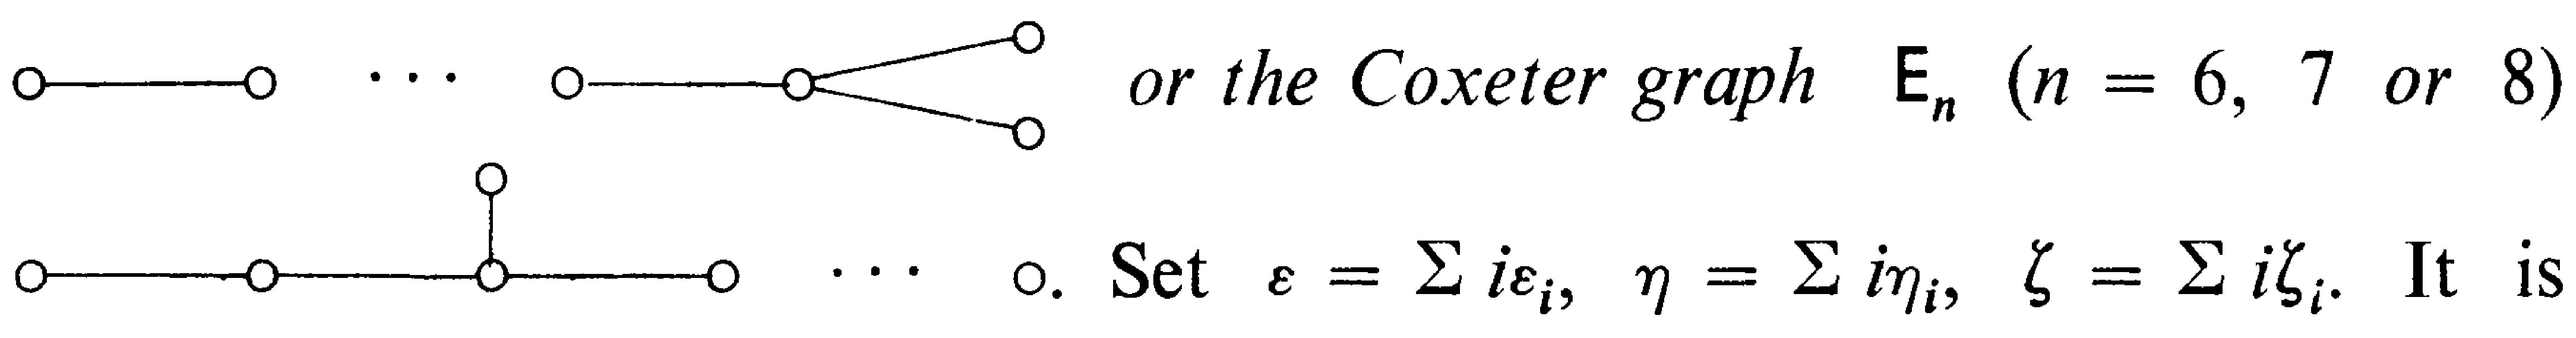
\includegraphics[max width=\textwidth, center]{2025_06_06_fac2836a92464059da43g-075(2)}\\
clear that $\varepsilon, \eta, \zeta$ are mutually orthogonal, linearly independent vectors, and that $\psi$ is not in their span. As in the proof of (4) we therefore obtain $\cos ^{2} \theta_{1}+\cos ^{2} \theta_{2}+\cos ^{2} \theta_{3}<1$, where $\theta_{1}, \theta_{2}, \theta_{3}$ are the respective angles between $\psi$ and $\varepsilon, \eta, \zeta$. The same calculation as in (9), with $p-1$ in place of $p$, shows that $(\varepsilon, \varepsilon)=p(p-1) / 2$, and similarly for $\eta$, $\zeta$. Therefore $\cos ^{2} \theta_{1}=$ $(\varepsilon, \psi)^{2} /(\varepsilon, \varepsilon) \quad(\psi, \psi)=(p-1)^{2}\left(\varepsilon_{p-1}, \psi\right)^{2} /(\varepsilon, \varepsilon)=\frac{1}{4}\left(2(p-1)^{2} / p(p-1)\right)=$ $(p-1) / 2 p=\frac{1}{2}(1-1 / p)$. Similarly for $\theta_{2}, \theta_{3}$. Adding, we get the inequality $\frac{1}{2}(1-1 / p+1-1 / q+1-1 / r)<1$, or $\left(^{*}\right) 1 / p+1 / q+1 / r>1$. (This inequality, by the way, has a long mathematical history.) By changing labels we may assume that $1 / p \leq 1 / q \leq 1 / r$ ( $\leq 1 / 2$; if $p, q$, or $r$ equals 1 , we are back in type $\mathrm{A}_{n}$ ). In particular, the inequality (*) implies $3 / 2 \geq 3 / r>1$, so $r=2$. Then $1 / p+1 / q>1 / 2,2 / q>1 / 2$, and $2 \leq q<4$. If $q=3$, then $1 / p>1 / 6$ and necessarily $p<6$. So the possible triples ( $p, q, r$ ) turn out to be: $(p, 2,2)$ $=\mathrm{D}_{n} ;(3,3,2)=\mathrm{E}_{6} ;(4,3,2)=\mathrm{E}_{7} ;(5,3,2)=\mathrm{E}_{8}$.

The preceding argument shows that the connected graphs of admissible sets of vectors in euclidean space are all to be found among the Coxeter graphs of types $\mathrm{A}-\mathrm{G}$. In particular, the Coxeter graph of a root system must be of one of these types. But in all cases except $\mathrm{B}_{\ell}, \mathrm{C}_{\ell}$, the Coxeter graph\\
uniquely determines the Dynkin diagram, as remarked at the outset. So the theorem follows.

\section*{Exercises}
\begin{enumerate}
  \item Verify the Cartan matrices (Table 1).
  \item Calculate the determinants of the Cartan matrices (using induction on $\ell$ for types $\mathrm{A}_{\ell}-\mathrm{D}_{\ell}$ ), which are as follows:
\end{enumerate}

$$
\mathrm{A}_{\ell}: \ell+1 ; \mathrm{B}_{\ell}: 2 ; \mathrm{C}_{\ell}: 2 ; \mathrm{D}_{\ell}: 4 ; \mathrm{E}_{6}: 3 ; \mathrm{E}_{7}: 2 ; \mathrm{E}_{8}, \mathrm{~F}_{4} \text { and } \mathrm{G}_{2}: 1 .
$$

\begin{enumerate}
  \setcounter{enumi}{2}
  \item Use the algorithm of (11.1) to write down all roots for $G_{2}$. Do the same for $C_{3}:\left(\begin{array}{rrr}2 & -1 & 0 \\ -1 & 2 & -1 \\ 0 & -2 & 2\end{array}\right)$.
  \item Prove that the Weyl group of a root system $\Phi$ is isomorphic to the direct product of the respective Weyl groups of its irreducible components.
  \item Prove that each irreducible root system is isomorphic to its dual, except that $\mathrm{B}_{\ell}, \mathrm{C}_{\ell}$ are dual to each other.
  \item Prove that an inclusion of one Dynkin diagram in another (e.g., $\mathrm{E}_{6}$ in $\mathrm{E}_{7}$ or $E_{7}$ in $E_{8}$ ) induces an inclusion of the corresponding root systems.
\end{enumerate}

\section*{Notes}
Our proof of the classification theorem follows Jacobson [1]. For a somewhat different approach, see Carter [1]. Bourbaki [2] emphasizes the classification of Coxeter groups, of which the Weyl groups of root systems are important examples.

\section*{12. Construction of root systems and automorphisms}
In §11 the possible (connected) Dynkin diagrams of (irreducible) root systems were all determined. It remains to be shown that each diagram of type A-G does in fact belong to a root system $\Phi$. Afterwards we shall briefly discuss Aut $\Phi$. The existence of root systems of type $A_{\ell}-D_{\ell}$ could actually be shown by verifying for each classical linear Lie algebra (1.2) that its root system is of the indicated type, which of course requires that we first prove the semisimplicity of these algebras (cf. §19). But it is easy enough to give a direct construction of the root system, which moreover makes plain the structure of its Weyl group.

\subsection*{12.1. Construction of types $\mathrm{A}-\mathrm{G}$}
We shall work in various spaces $\mathbf{R}^{n}$, where the inner product is the usual one and where $\varepsilon_{1}, \ldots, \varepsilon_{n}$ denote the usual orthonormal unit vectors which\\
form a basis of $\mathbf{R}^{n}$. The $\mathbf{Z}$-span of this basis is (by definition) a lattice, denoted I. In each case we shall take E to be $\mathbf{R}^{n}$ (or a suitable subspace thereof, with the inherited inner product). Then $\Phi$ will be defined to be the set of all vectors in $I$ (or a closely related subgroup $J$ of E) having specified length or lengths.

Since the group $I$ (or $J$ ) is discrete in the usual topology of $\mathbf{R}^{n}$, while the set of vectors in $\mathbf{R}^{n}$ having one or two given lengths is compact (closed and bounded), $\Phi$ is then obviously finite, and will exclude 0 by definition. In each case it will be evident that $\Phi$ spans E (indeed, a base of $\Phi$ will be exhibited explicitly). Therefore (R1) is satisfied. The choice of lengths will also make it obvious that (R2) holds. For (R3) it is enough to check that the reflection $\sigma_{\alpha}(\alpha \in \Phi)$ maps $\Phi$ back into $J$, since then $\sigma_{\alpha}(\Phi)$ automatically consists of vectors of the required lengths. But then (R3) follows from (R4). As to (R4), it usually suffices to choose squared lengths dividing 2 , since it is automatic that all inner products $(\alpha, \beta) \in \mathbf{Z}(\alpha, \beta \in I)$.

Having made these preliminary remarks, we now treat the separate cases A-G. After verifying (R1) to (R4) in the way just sketched, the reader should observe that the resulting Cartan matrix matches that in Table 1 (11.4).\\
$\mathrm{A}_{\ell}(\ell \geq 1)$ : Let E be the $\ell$-dimensional subspace of $\mathbf{R}^{\ell+1}$ orthogonal to the vector $\varepsilon_{1}+\ldots+\varepsilon_{\ell+1}$. Let $I^{\prime}=I \cap \mathrm{E}$, and take $\Phi$ to be the set of all vectors $\alpha \in I^{\prime}$ for which ( $\alpha, \alpha$ ) $=2$. It is obvious that $\Phi=\left\{\varepsilon_{i}-\varepsilon_{j}, i \neq j\right\}$. The vectors $\alpha_{i}=\varepsilon_{i}-\varepsilon_{i+1}(1 \leq i \leq \ell)$ are independent, and $\varepsilon_{i}-\varepsilon_{j}=\left(\varepsilon_{i}-\varepsilon_{i+1}\right)$ $+\left(\varepsilon_{i+1}-\varepsilon_{i+2}\right)+\ldots+\left(\varepsilon_{j-1}-\varepsilon_{j}\right)$ if $i<j$, which shows that they form a base of $\Phi$. It is clear that the Cartan matrix $A$, results. Finally, notice that the reflection with respect to $\alpha_{i}$ permutes the subscripts $i, i+1$ and leaves all other subscripts fixed. Thus $\sigma_{\alpha_{i}}$ corresponds to the transposition $(i, i+1)$ in the symmetric group $\mathscr{S}_{l+1}$; these transpositions generate $\mathscr{S}_{l+1}$, so we obtain a natural isomorphism of $\mathscr{W}$ onto $\mathscr{S}_{\ell+1}$.\\
$\mathrm{B}_{\ell}(\ell \geq 2)$ : Let $\mathrm{E}=\mathbf{R}^{\ell}, \Phi=\{\alpha \in I \mid(\alpha, \alpha)=1$ or 2$\}$. It is easy to check that $\Phi$ consists of the vectors $\pm \varepsilon_{i}$ (of squared length 1) and the vectors $\pm\left(\varepsilon_{i} \pm \varepsilon_{j}\right), i \neq j$ (of squared length 2). The $\ell$ vectors $\varepsilon_{1}-\varepsilon_{2}, \varepsilon_{2}-\varepsilon_{3}, \ldots, \varepsilon_{\ell-1}$ $-\varepsilon_{\ell}, \varepsilon_{\ell}$ are independent; a short root $\varepsilon_{i}=\left(\varepsilon_{i}-\varepsilon_{i+1}\right)+\left(\varepsilon_{i+1}-\varepsilon_{i+2}\right)+\ldots$ $+\left(\varepsilon_{\ell-1}-\varepsilon_{\ell}\right)+\varepsilon_{\ell}$, while a long root $\varepsilon_{i}-\varepsilon_{j}$ or $\varepsilon_{i}+\varepsilon_{j}$ is similarly expressible. The Cartan matrix for this (ordered) base is clearly $\mathrm{B}_{\ell} . \mathscr{W}$ acts as the group of all permutations and sign changes of the set $\left\{\varepsilon_{1}, \ldots, \varepsilon_{\ell}\right\}$, so $\mathscr{W}$ is isomorphic to the semidirect product of $(\mathbf{Z} / 2 \mathbf{Z})^{\ell}$ and $\mathscr{S}_{\ell}$ (the latter acting on the former).\\
$\mathrm{C}_{\ell}(\ell \geq 3): \mathrm{C}_{\ell}(\ell \geq 2)$ may be viewed most conveniently as the root system dual to $B_{\ell}$ (with $B_{2}=C_{2}$ ), cf. Exercise 11.5. The reader can verify directly that in $\mathrm{E}=\mathbf{R}^{\prime}$, the set of all $\pm 2 \varepsilon_{i}$ and all $\pm\left(\varepsilon_{i} \pm \varepsilon_{j}\right), i \neq j$, forms a root system of type $C_{\ell}$, with base $\left(\varepsilon_{1}-\varepsilon_{2}, \ldots, \varepsilon_{\ell-1}-\varepsilon_{\ell}, 2 \varepsilon_{\ell}\right\}$. Of course the Weyl group is isomorphic to that of $\mathrm{B}_{l}$.

$$
\mathrm{D}_{\ell}(\ell \geq 4): \text { Let } \mathrm{E}=\mathbf{R}^{\ell}, \Phi=\{\alpha \in I \mid(\alpha, \alpha)=2\}=\left\{ \pm\left(\varepsilon_{i} \pm \varepsilon_{\jmath}\right), i \neq j\right\} .
$$

For a base take the $\ell$ independent vectors $\varepsilon_{1}-\varepsilon_{2}, \ldots, \varepsilon_{\ell-1}-\varepsilon_{\ell}, \varepsilon_{\ell-1}+\varepsilon_{\ell}$ (so $D_{\ell}$ results). The Weyl group is the group of permutations and sign changes\\
involving only even numbers of signs of the set $\left\{\varepsilon_{1}, \ldots, \varepsilon_{\ell}\right\}$. So $\mathscr{W}$ is isomorphic to the semidirect product of $(\mathbf{Z} / 2 \mathbf{Z})^{\rho-1}$ and $\mathscr{S}_{\rho}$.\\
$E_{6}, E_{7}, E_{8}$ : We know that $E_{6}, E_{7}$ can be identified canonically with subsystems of $\mathrm{E}_{8}$ (Exercise 11.6), so it suffices to construct $\mathrm{E}_{8}$. This is slightly complicated. Take $\mathbf{E}=\mathbf{R}^{8}, I^{\prime}=I+\mathbf{Z}\left(\left(\varepsilon_{1}+\ldots+\varepsilon_{8}\right) / 2\right), I^{\prime \prime}=$ subgroup of $I^{\prime}$ consisting of all elements $\Sigma c_{i} \varepsilon_{i}+\frac{c}{2}\left(\varepsilon_{1}+\ldots+\varepsilon_{8}\right)$ for which $c+\Sigma c_{i}$ is an even integer. (Check that this is a subgroup!) Define $\Phi=\left\{\alpha \in I^{\prime \prime} \mid(\alpha, \alpha)=2\right\}$. It is easy to see that $\Phi$ consists of the obvious vectors $\pm\left(\varepsilon_{i} \pm \varepsilon_{j}\right), i \neq j$, along with the less obvious ones $\frac{1}{2} \sum_{i=1}^{8}(-1)^{h(i)} \varepsilon_{i}$ (where the $k(i)=0,1$, add up to an even integer). By inspection, all inner products here are in $\mathbf{Z}$ (this has to be checked, because we are working in a larger lattice than $I$ ). As a base we take $\left\{\frac{1}{2}\left(\varepsilon_{1}+\varepsilon_{8}-\left(\varepsilon_{2}+\ldots+\varepsilon_{7}\right)\right), \varepsilon_{1}+\varepsilon_{2}, \varepsilon_{2}-\varepsilon_{1}, \varepsilon_{3}-\varepsilon_{2}, \varepsilon_{4}-\varepsilon_{3}, \varepsilon_{5}-\varepsilon_{4}, \varepsilon_{6}-\varepsilon_{5}\right.$, $\left.\varepsilon_{7}-\varepsilon_{6}\right\}$. (This has been crdered so as to correspond to the Cartan matrix for $\mathrm{E}_{8}$ in Table 1 (11.4).) The reader is invited to contemplate for himself the action of the Weyl group, whose order can be shown to be $2^{14} 3^{5} 5^{2} 7$.\\
$\mathrm{F}_{4}$ : Let $\mathrm{E}=\mathbf{R}^{4}, I^{\prime}=I+\mathbf{Z}\left(\left(\varepsilon_{1}+\varepsilon_{2}+\varepsilon_{3}+\varepsilon_{4}\right) / 2\right), \Phi=\left\{\alpha \in I^{\prime} \mid(\alpha, \alpha)=1\right.$ or $2\}$. Then $\Phi$ consists of all $\pm \varepsilon_{i}$, all $\pm\left(\varepsilon_{i} \pm \varepsilon_{j}\right), i \neq j$, as well as all $\pm \frac{1}{2}\left(\varepsilon_{1} \pm \varepsilon_{2}\right.$ $\pm \varepsilon_{3} \pm \varepsilon_{4}$ ), where the signs may be chosen independently. By inspection, all numbers $\langle\alpha, \beta\rangle$ are integral. As a base take $\left\{\varepsilon_{2}-\varepsilon_{3}, \varepsilon_{3}-\varepsilon_{4}, \varepsilon_{4}, \frac{1}{2}\left(\varepsilon_{1}-\varepsilon_{2}-\varepsilon_{3}\right.\right.$ $\left.\left.-\varepsilon_{4}\right)\right\}$. Here $\mathscr{W}$ has order 1152 .\\
$\mathrm{G}_{2}$ : We already constructed $\mathrm{G}_{2}$ explicitly in $\S$. Abstractly, we can take E to be the subspace of $\mathbf{R}^{3}$ orthogonal to $\varepsilon_{1}+\varepsilon_{2}+\varepsilon_{3}, I^{\prime}=I \cap \mathrm{E}, \Phi=$ $\left\{\alpha \in I^{\prime} \mid(\alpha, \alpha)=2\right.$ or 6$\}$. So $\Phi= \pm\left\{\varepsilon_{1}-\varepsilon_{2}, \varepsilon_{2}-\varepsilon_{3}, \varepsilon_{1}-\varepsilon_{3}, 2 \varepsilon_{1}-\varepsilon_{2}-\varepsilon_{3}\right.$, $\left.2 \varepsilon_{2}-\varepsilon_{1}-\varepsilon_{3}, 2 \varepsilon_{3}-\varepsilon_{1}-\varepsilon_{2}\right\}$. As a base choose $\varepsilon_{1}-\varepsilon_{2},-2 \varepsilon_{1}+\varepsilon_{2}+\varepsilon_{3}$. (How does $\mathscr{W}$ act?)

Theorem. For each Dynk in diagram (or Cartan matrix) of type A-G, there exists an irreducible root system having the given diagram.

\subsection*{12.2. Automorphisms of $\mathbf{\Phi}$}
We are going to give a complete description of Aut $\Phi$, for each root system $\Phi$. Recall that Lemma 9.2 implies that $\mathscr{W}$ is a normal subgroup of Aut $\Phi$ (Exercise 9.6). Let $\Gamma=\{\sigma \in$ Aut $\Phi \mid \sigma(\Delta)=\Delta\}, \Delta$ a fixed base of $\Phi$. Evidently, $\Gamma$ is a subgroup of Aut $\Phi$. If $\tau \in \Gamma \cap \mathscr{W}$, then $\tau=1$ by virtue of the simple transitivity of $\mathscr{W}$ (Theorem 10.3(e)). Moreover, if $\tau \in$ Aut $\Phi$ is arbitrary, then $\tau(\Delta)$ is evidently another base of $\Phi$, so there exists $\sigma \in \mathscr{W}$ such that $\sigma \tau(\Delta)=\Delta$ (Theorem 10.3(b)), whence $\tau \in \Gamma \mathscr{W}$. It follows that Aut $\Phi$ is the semidirect product of $\Gamma$ and $\mathscr{W}$.

For all $\tau \in$ Aut $\Phi$, all $\alpha, \beta \in \Phi$, we have $\langle\alpha, \beta\rangle=\langle\tau(\alpha), \tau(\beta)\rangle$. Therefore, each $\tau \in \Gamma$ determines an automorphism (in the obvious sense) of the Dynkin diagram of $\Phi$. If $\tau$ acts trivially on the diagram, then $\tau=1$ (because $\Delta$ spans E). On the other hand, each automorphism of the Dynkin diagram obviously determines an automorphism of $\Phi$ (cf. Proposition 11.1). So $\Gamma$ may be

Table 1.

\begin{center}
\begin{tabular}{|l|l|l|l|l|}
\hline
Type & Number of Positive Roots & Order of $\mathscr{W}$ & Structure of $\mathscr{W}$ & $\Gamma$ \\
\hline
$\mathrm{A}_{l}$ & $\binom{\ell+1}{2}$ & $(\ell+1)!$ & $\mathscr{S}_{t+1}$ & $\mathrm{Z} / 2 \mathrm{Z}(\ell \geq 2)$ \\
\hline
$\mathrm{B}_{\ell}, \mathrm{C}_{\ell}$ & $t^{2}$ & $2^{t}$ ! & $(\mathbf{Z} / 2 \mathbf{Z})^{\ell}>\mathscr{S}_{t}$ & 1 \\
\hline
$\mathrm{D}_{\ell}$ & $\ell^{2}-\ell$ & $2^{\ell-1} \ell!$ & $(\mathbf{Z} / 2 \mathbf{Z})^{\ell-1}>\mathscr{S}_{\ell}$ & $\left\{\begin{array}{cl}\mathscr{S}_{3} & (\ell=4) \\ \mathbf{Z} / 2 \mathbf{Z} & (\ell>4)\end{array}\right.$ \\
\hline
$\mathrm{E}_{6}$ & 36 & 27345 &  & Z/2Z \\
\hline
$\mathrm{E}_{7}$ & 63 & 2103457 &  & 1 \\
\hline
$\mathrm{E}_{8}$ & 120 & 21435527 &  & 1 \\
\hline
$\mathrm{F}_{4}$ & 24 & 2732 &  & 1 \\
\hline
$\mathrm{G}_{2}$ & 6 & 223 & $\mathscr{D}_{6}$ & 1 \\
\hline
\end{tabular}
\end{center}

identified with the group of diagram automorphisms. A glance at the list in (11.4) yields a description of $\Gamma$, summarized in Table 1 along with other useful data, for $\Phi$ irreducible. (Since diagram automorphisms other than the identity exist only in cases of single root length, when the Dynkin diagram and Coxeter graph coincide, the term graph automorphism may also be used.)

\section*{Exercises}
\begin{enumerate}
  \item Verify the details of the constructions in (12.1).
  \item Verify Table 2.
  \item Let $\Phi \subset E$ satisfy (R1), (R3), (R4), but not (R2), cf. Exercise 9.9. Suppose moreover that $\Phi$ is irreducible, in the sense of §11. Prove that $\Phi$ is the union of root systems of type $\mathrm{B}_{n}, \mathrm{C}_{n}$ in $\mathrm{E}(n=\operatorname{dim} \mathrm{E})$, where the long roots of $\mathrm{B}_{n}$ are also the short roots of $\mathrm{C}_{n}$. (This is called the non-reduced root system of type $\mathrm{BC}_{n}$ in the literature.)
\end{enumerate}

Table 2. Highest long and short roots

\begin{center}
\begin{tabular}{|l|l|l|}
\hline
Type & Long & Short \\
\hline
$\mathrm{A}_{\ell}$ & $\alpha_{1}+\alpha_{2}+\ldots+\alpha_{l}$ &  \\
\hline
$\mathrm{B}_{\ell}$ & $\alpha_{1}+2 \alpha_{2}+2 \alpha_{3}+\ldots+2 \alpha_{l}$ & $\alpha_{1}+\alpha_{2}+\ldots+\alpha_{1}$ \\
\hline
$\mathrm{C}_{\ell}$ & $2 \alpha_{1}+2 \alpha_{2}+\ldots+2 \alpha_{\ell-1}+\alpha_{\ell}$ & $\alpha_{1}+2 \alpha_{2}+\ldots+2 \alpha_{l-1}+\alpha_{l}$ \\
\hline
$\mathrm{D}_{\ell}$ & $\alpha_{1}+2 \alpha_{2}+\ldots+2 \alpha_{\ell-2}+\alpha_{\ell-1}+\alpha_{\ell}$ &  \\
\hline
$\mathrm{E}_{6}$ & $\alpha_{1}+2 \alpha_{2}+2 \alpha_{3}+3 \alpha_{4}+2 \alpha_{5}+\alpha_{6}$ &  \\
\hline
$E_{7}$ & $2 \alpha_{1}+2 \alpha_{2}+3 \alpha_{3}+4 \alpha_{4}+3 \alpha_{5}+2 \alpha_{6}+\alpha_{7}$ &  \\
\hline
$\mathrm{E}_{8}$ & $2 \alpha_{1}+3 \alpha_{2}+4 \alpha_{3}+6 \alpha_{4}+5 \alpha_{5}+4 \alpha_{6}+3 \alpha_{7}+2 \alpha_{8}$ &  \\
\hline
$F_{4}$ & $2 \alpha_{1}+3 \alpha_{2}+4 \alpha_{3}+2 \alpha_{4}$ & $\alpha_{1}+2 \alpha_{2}+3 \alpha_{3}+2 \alpha_{4}$ \\
\hline
$\mathrm{G}_{2}$ & $3 \alpha_{1}+2 \alpha_{2}$ & $2 \alpha_{1}+\alpha_{2}$ \\
\hline
\end{tabular}
\end{center}

\begin{enumerate}
  \setcounter{enumi}{3}
  \item Prove that the long roots in $G_{2}$ form a root system in $E$ of type $A_{2}$.
  \item In constructing $\mathrm{C}_{\ell}$, would it be correct to characterize $\Phi$ as the set of all vectors in $I$ of squared length 2 or 4 ? Explain.
  \item Prove that the map $\alpha \mapsto-\alpha$ is an automorphism of $\Phi$. Try to decide for which irreducible $\Phi$ this belongs to the Weyl group.
  \item Describe Aut $\Phi$ when $\Phi$ is not irreducible.
\end{enumerate}

\section*{Notes}
The treatment here follows Serre [2]. More information about the individual root systems may be found in Bourbaki [2].

\section*{13. Abstract theory of weights}
In this section we describe that part of the representation theory of semisimple Lie algebras which depends only on the root system. (None of this is needed until Chapter VI.) Let $\Phi$ be a root system in a euclidean space E, with Weyl group $\mathscr{W}$.

\subsection*{13.1. Weights}
Let $\Lambda$ be the set of all $\lambda \in \mathrm{E}$ for which $\langle\lambda, \alpha\rangle \in \mathbf{Z}(\alpha \in \Phi)$, and call its elements weights. Since $\langle\lambda, \alpha\rangle=\frac{2(\lambda, \alpha)}{(\alpha, \alpha)}$ depends linearly on $\lambda, \Lambda$ is a subgroup of $\mathbf{E}$ including $\Phi$. Thanks to Exercise 10.1, $\lambda \in \Lambda$ iff $\langle\lambda, \alpha\rangle \in \mathbf{Z}$ for all $\alpha \in \Delta$. Denote by $\Lambda_{r}$ the root lattice ( $=$ subgroup of $\Lambda$ generated by $\Phi$ ). $\Lambda_{r}$ is a lattice in $\mathbf{E}$ in the technical sense: it is the $\mathbf{Z}$-span of an $\mathbf{R}$-basis of $\mathbf{E}$ (namely, any set of simple roots). Fix a base $\Delta \subset \Phi$, and define $\lambda \in \Lambda$ to be dominant if all the integers $\langle\lambda, \alpha\rangle(\alpha \in \Delta)$ are nonnegative, strongly dominant if these integers are positive. Let $\Lambda^{+}$be the set of all dominant weights. In the language of (10.1), $\Lambda^{+}$is the set of all weights lying in the closure of the fundamental Weyl chamber $\mathfrak{C}(\Delta)$, while $\Lambda \cap \mathfrak{C}(\Delta)$ is the set of strongly dominant weights.

It $\Delta=\left\{\alpha_{1}, \ldots, \alpha_{\ell}\right\}$, then the vectors $2 \alpha_{i} /\left(\alpha_{i}, \alpha_{i}\right)$ again form a basis of $E$. Let $\lambda_{1}, \ldots, \lambda_{\ell}$ be the dual basis (relative to the inner product on $E$ ): $\frac{2\left(\lambda_{i}, \alpha_{j}\right)}{\left(\alpha_{j}, \alpha_{j}\right)}=\delta_{i j}$. Since all $\left\langle\lambda_{i}, \alpha\right\rangle(\alpha \in \Delta)$ are nonnegative integers, the $\lambda_{i}$ are dominant weights. We call them the fundamental dominant weights (relative to $\Delta$ ). Notice that $\sigma_{i} \lambda_{j}=\lambda_{j}-\delta_{i j} \alpha_{i}$. If $\lambda \in \mathrm{E}$ is arbitrary, e.g., any weight, let $m_{i}=\left\langle\lambda, \alpha_{i}\right\rangle$. Then $0=\left\langle\lambda-\Sigma m_{i} \lambda_{i}, \alpha\right\rangle$ for each simple root $\alpha$, which implies that $\left(\lambda-\Sigma m_{i} \lambda_{i}, \alpha\right)=0$ as well, or that $\lambda=\Sigma m_{i} \lambda_{i}$. Therefore, $\Lambda$ is a lattice with basis $\left(\lambda_{i}, 1 \leq i \leq \ell\right.$ ), and $\lambda \in \Lambda^{+}$if and only if all $m_{i} \geq 0$. (Cf. Figure 1, for type $\mathrm{A}_{2}$.)\\
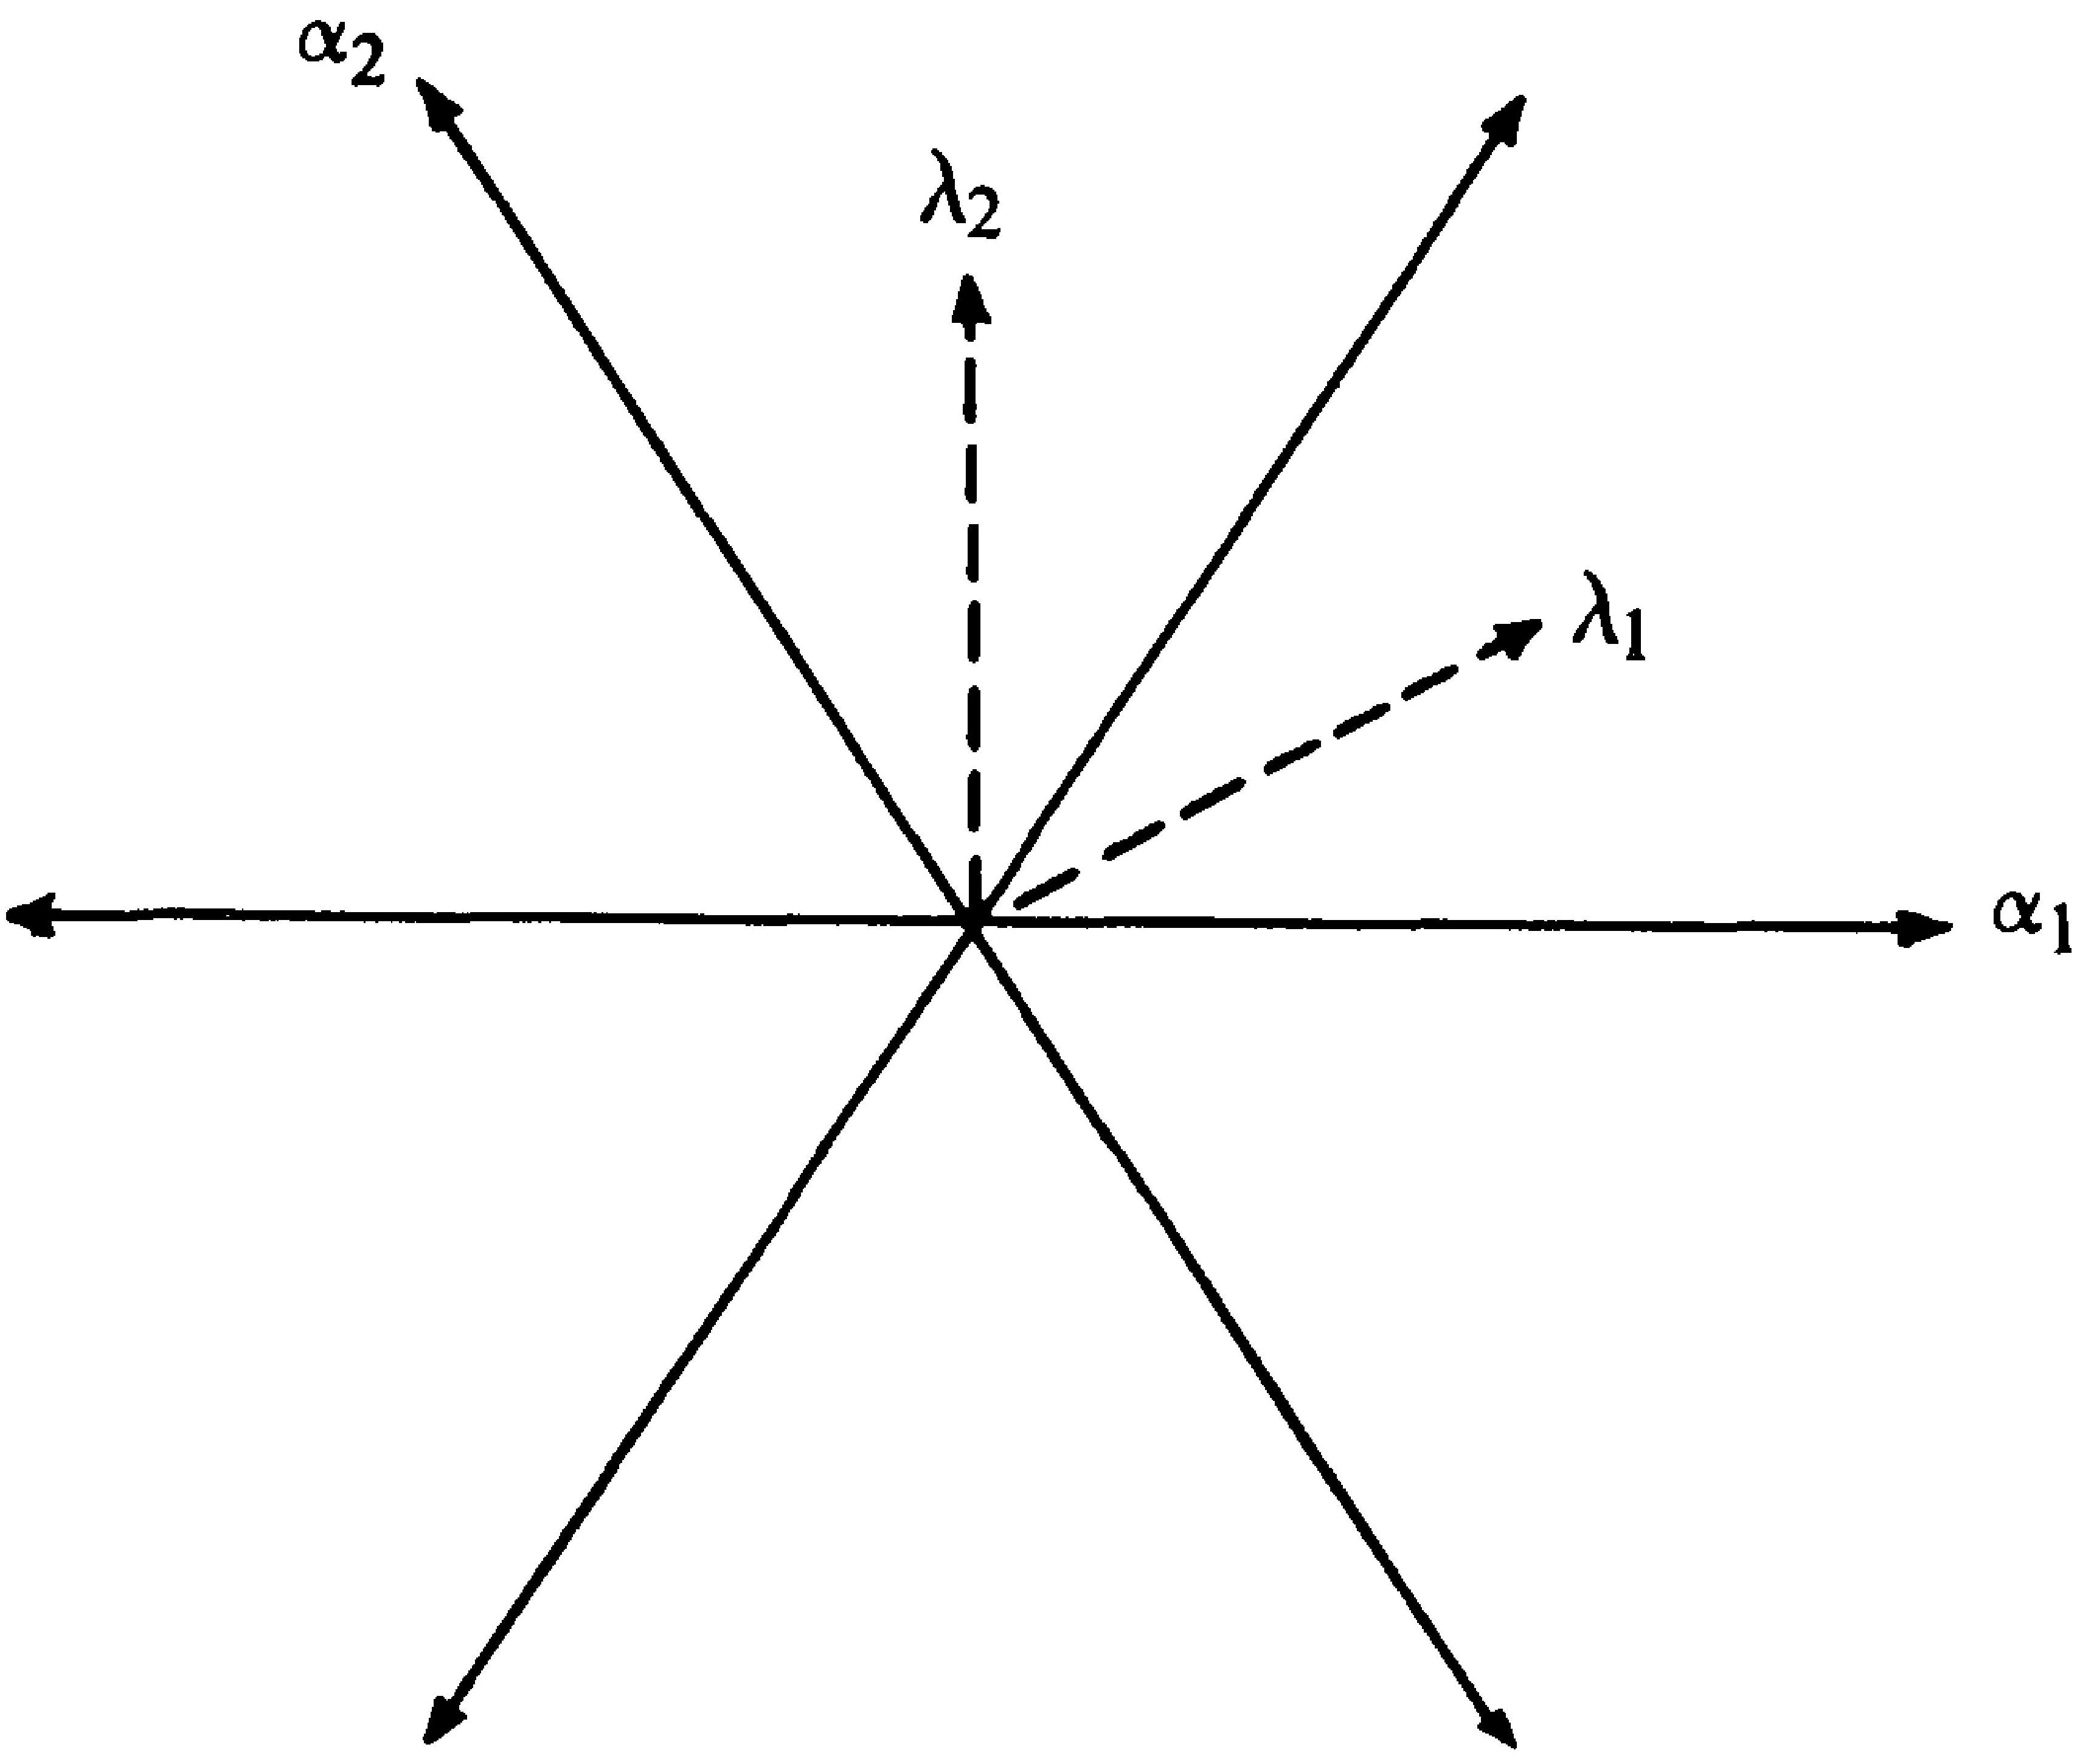
\includegraphics[max width=\textwidth, center]{2025_06_06_fac2836a92464059da43g-081}

Figure 1

It is an elementary fact about lattices that $\Lambda / \Lambda_{r}$ must be a finite group (called the fundamental group of $\Phi$ ). We can see this directly as follows. Write $\alpha_{i}=\sum_{j} m_{i j} \lambda_{j}\left(m_{i j} \in \mathbf{Z}\right)$. Then $\left\langle\alpha_{i}, \alpha_{k}\right\rangle=\sum_{j} m_{i j}\left\langle\lambda_{j}, \alpha_{k}\right\rangle=m_{i k}$. In other words, the Cartan matrix expresses the change of basis. To write the $\lambda_{j}$ in terms of the $\alpha_{i}$, we have only to invert the Cartan matrix; its determinant (cf. Exercise 11.2) is the sole denominator involved, so this measures the index of $\Lambda_{r}$ in $\Lambda$. For example, in type $\mathrm{A}_{1}, \alpha_{1}=2 \lambda_{1}$. (This is the only case in which a simple root is dominant, for reasons which will later become apparent.) In type $A_{2}$, the Cartan matrix is $\left(\begin{array}{rr}2 & -1 \\ -1 & 2\end{array}\right)$, so $\alpha_{1}=2 \lambda_{1}-\lambda_{2}$ and $\alpha_{2}=-\lambda_{1}+2 \lambda_{2}$. Inverting, we get $(1 / 3)\left(\begin{array}{ll}2 & 1 \\ 1 & 2\end{array}\right)$, so that $\lambda_{1}=(1 / 3)$ ( $2 \alpha_{1}+\alpha_{2}$ ) and $\lambda_{2}=(1 / 3)\left(\alpha_{1}+2 \alpha_{2}\right)$. By computing determinants of Cartan matrices one verifies the following list of orders for the fundamental groups $\Lambda / \Lambda_{r}$ in the irreducible cases:

$$
\mathrm{A}_{\ell}, \ell+1 ; \mathrm{B}_{\ell}, \mathrm{C}_{\ell}, \mathrm{E}_{7}, 2 ; \mathrm{D}_{\ell}, 4 ; \mathrm{E}_{6}, 3 ; \mathrm{E}_{8}, \mathrm{~F}_{4}, \mathrm{G}_{2}, 1 .
$$

With somewhat more labor one can calculate explicitly the $\lambda_{i}$ in terms of the $\alpha_{j}$. This information is listed in Table 1, for the reader's convenience, although strictly speaking we shall not need it in what follows. The exact structure of the fundamental group can be found by computing elementary divisors, or can be deduced from Table 1 once the latter is known (Exercise 4).

\subsection*{13.2. Dominant weights}
The Weyl group $\mathscr{W}$ of $\Phi$ preserves the inner product on $E$, hence leaves $\Lambda$ invariant. (In fact, we already made the more precise observation that $\sigma_{i} \lambda_{j}=\lambda_{j}-\delta_{i j} \alpha_{i}$.) Orbits of weights under $\mathscr{W}$ occur frequently in the study of representations. In view of Lemma 10.3B and Exercise 10.14, we can state:

Lemma A. Each weight is conjugate under $\mathscr{W}$ to one and only one dominant weight. If $\lambda$ is dominant, then $\sigma \lambda \prec \lambda$ for all $\sigma \in \mathscr{W}$, and if $\lambda$ is strongly dominant, then $\sigma \lambda=\lambda$ only when $\sigma=1$.

As a subset of $E, \Lambda$ is partially ordered by the relation: $\lambda>\mu$ if and only if $\lambda-\mu$ is a sum of positive roots (10.1). Unfortunately, this ordering does not have too close a connection with the property of being dominant; for example, it is easy to have $\mu$ dominant, $\mu \prec \lambda$, but $\lambda$ not dominant (Exercise 2). Our next lemma shows, however, that dominant weights are not too badly behaved relative to $\prec$.

Table 1.

\begin{verbatim}
$\mathrm{A}_{\ell}: \quad \lambda_{i}=\frac{1}{\ell+1}\left[(\ell-i+1) \alpha_{1}+2(\ell-i+1) \alpha_{2}+\ldots+(i-1)(\ell-i+1) \alpha_{i-1}\right.$
    $\left.+i(\ell-i+1) \alpha_{i}+i(\ell-i) \alpha_{i+1}+\ldots+i \alpha_{\ell}\right]$
$\mathrm{B}_{\ell}: \quad \lambda_{i}=\alpha_{1}+2 \alpha_{2}+\ldots+(i-1) \alpha_{i-1}+i\left(\alpha_{i}+\alpha_{i+1}+\ldots+\alpha_{\ell}\right) \quad(i</)$
    $\lambda_{f}=\frac{1}{2}\left(\alpha_{1}+2 \alpha_{2}+\ldots+\left(\alpha_{f}\right)\right.$
$\mathrm{C}_{\ell}: \quad \lambda_{i}=\alpha_{1}+2 \alpha_{2}+\ldots+(i-1) \alpha_{i-1}+i\left(\alpha_{i}+\ldots+\alpha_{f-1}+\frac{1}{2} \alpha_{f}\right)$
$\mathrm{D}_{\ell}: \quad \lambda_{i}=\alpha_{1}+2 \alpha_{2}+\ldots+(i-1) \alpha_{i-1}+i\left(\alpha_{i}+\ldots+\alpha_{\ell-2}\right)+\frac{1}{2} i\left(\alpha_{\ell-1}+\alpha_{\ell}\right) \quad(i<\ell-1)$
    $\lambda_{f-1}=\frac{1}{2}\left(\alpha_{1}+2 \alpha_{2}+\ldots+(f-2) \alpha_{f-2}+\frac{1}{2}\left(\alpha_{f-1}+\frac{1}{2}(f-2) \alpha_{f}\right)\right.$
        $\lambda_{f}=\frac{1}{2}\left(\alpha_{1}+2 \alpha_{2}+\ldots+(f-2) \alpha_{f-2}+\frac{1}{2}(f-2) \alpha_{f-1}+\frac{1}{2}\left(\alpha_{f}\right)\right.$
( $\Sigma q_{i} x_{i}$ is abbreviated ( $q_{1}, \ldots q_{\ell}$ ) in the following lists.)
$\mathrm{E}_{6}: \quad \lambda_{1}=\frac{1}{3}(4,3,5,6,4,2)$
    $\lambda_{2}=(1,2,2,3,2,1)$
    $\lambda_{3}=\frac{1}{3}(5,6,10,12,8,4)$
    $\lambda_{4}=(2,3,4,6,4,2)$
    $\lambda_{5}=\frac{1}{3}(4,6,8,12,10,5)$
    $\lambda_{6}=\frac{1}{3}(2,3,4,6,5,4)$
$\mathrm{E}_{7}: \lambda_{1}=(2,2,3,4,3,2,1)$
    $\lambda_{2}=\frac{1}{2}(4,7,8,12,9,6,3)$
    $\lambda_{3}=(3,4,6,8,6,4,2)$
    $\lambda_{4}=(4,6,8,12,9,6,3)$
    $\lambda_{5}=\frac{1}{2}(6,9,12,18,15,10,5)$
    $\lambda_{6}=(2,3,4,6,5,4,2)$
    $\lambda_{7}=\frac{1}{2}(2,3,4,6,5,4,3)$
$\mathrm{E}_{8}: \lambda_{1}=(4,5,7,10,8,6,4,2)$
    $\lambda_{2}=(5,8,10,15,12,9,6,3)$
    $\lambda_{3}=(7,10,14,20,16,12,8,4)$
    $\lambda_{4}=(10,15,20,30,24,18,12,6)$
    $\lambda_{5}=(8,12,16,24,20,15,10,5)$
    $\lambda_{6}=(6,9,12,18,15,12,8,4)$
    $\lambda_{7}=(4,6,8,12,10,8,6,3)$
    $\lambda_{8}=(2,3,4,6,5,4,3,2)$
$\mathrm{F}_{4}: \quad \lambda_{1}=(2,3,4,2)$
    $\lambda_{2}=(3,6,8,4)$
    $\lambda_{3}=(2,4,6,3)$
    $\lambda_{4}=(1,2,3,2)$
$\mathrm{G}_{2}: \lambda_{1}=(2,1)$
    $\lambda_{2}=(3,2)$
\end{verbatim}

Lemma B. Let $\lambda \in \Lambda^{+}$. Then the number of dominant weights $\mu \prec \lambda$ is finite.\\
Proof. Since $\lambda+\mu \in \Lambda^{+}$and $\lambda-\mu$ is a sum of positive roots, $0 \leq(\lambda+\mu, \lambda$ $-\mu)=(\lambda, \lambda)-(\mu, \mu)$. Thus $\mu$ lies in the compact set $\{x \in \mathrm{E} \mid(x, x) \leq(\lambda, \lambda)\}$, whose intersection with the discrete set $\Lambda^{+}$is finite.

\subsection*{13.3. The weight $\delta$}
Recall (Corollary to Lemma 10.2B) that $\delta=\frac{1}{2} \sum_{\alpha>0} \alpha$, and that $\sigma_{i} \delta=\delta-\alpha_{i}$ ( $1 \leq i \leq \ell$ ). Of course, $\delta$ may or may not lie in the root lattice $\Lambda_{r}$ (cf. type $\mathrm{A}_{1}$ ); but $\delta$ does lie in $\Lambda$. More precisely:

Lemma A. $\delta=\sum_{j=1}^{\ell} \lambda_{j}$, so $\delta$ is a (strongly) dominant weight.\\
Proof. Since $\sigma_{i} \delta=\delta-\alpha_{i},\left(\delta-\alpha_{i}, \alpha_{i}\right)=\left(\sigma_{i}^{2} \delta, \sigma_{i} \alpha_{i}\right)=\left(\delta,-\alpha_{i}\right)$, or $2\left(\delta, \alpha_{i}\right)$ $=\left(\alpha_{i}, \alpha_{i}\right)$, or $\left\langle\delta, \alpha_{i}\right\rangle=1(1 \leq i \leq \ell)$. But $\delta=\sum_{i}\left\langle\delta, \alpha_{i}\right\rangle \lambda_{i}$ (cf. (13.1)), so the lemma follows.

The next lemma is merely an auxiliary result, needed in (13.4).\\
Lemma B. Let $\mu \in \Lambda^{+}, \nu=\sigma^{-1} \mu(\sigma \in \mathscr{W})$. Then $(\nu+\delta, \nu+\delta) \leq(\mu+\delta$, $\mu+\delta)$, with equality only if $\nu=\mu$.

Proof. $(\nu+\delta, \nu+\delta)=(\sigma(\nu+\delta), \sigma(\nu+\delta))=(\mu+\sigma \delta, \mu+\sigma \delta)=(\mu+\delta, \mu+$ $\delta)-2(\mu, \delta-\sigma \delta)$. Since $\mu \in \Lambda^{+}$, and $\delta-\sigma \delta$ is a sum of positive roots ( $13.2 \mathrm{~A}, 13.3 \mathrm{~A}$ ), the right side is $\leq(\mu+\delta, \mu+\delta)$, with equality only if $(\mu, \delta-\sigma \delta)=0$, i.e., $(\mu, \delta)=(\mu, \sigma \delta)=(\nu, \delta)$, or $(\mu-\nu, \delta)=0$. But $\mu-\nu$ is a sum of positive roots (13.2A) and $\delta$ is strongly dominant, so $\mu=\nu$.

\subsection*{13.4. Saturated sets of weights}
Certain finite sets of weights, stable under $\mathscr{W}$, play a prominent role in representation theory. We call a subset $\Pi$ of $\Lambda$ saturated if for all $\lambda \in \Pi$, $\alpha \in \Phi$, and $i$ between 0 and $\langle\lambda, \alpha\rangle$, the weight $\lambda-i \alpha$ also lies in $\Pi$. Notice first that any saturated set is automatically stable under $\mathscr{W}$, since $\sigma_{\alpha} \lambda=\lambda-$ $\langle\lambda, \alpha\rangle \alpha$ and $\mathscr{W}$ is generated by reflections. We say that a saturated set $\Pi$ has highest weight $\lambda\left(\lambda \in \Lambda^{+}\right)$if $\lambda \in \Pi$ and $\mu \prec \lambda$ for all $\mu \in \Pi$. Examples: (1) The set consisting of 0 alone is saturated, with highest weight 0 . (2) The set $\Phi$ of all roots of a semisimple Lie algebra, along with 0 , is saturated. In case $\Phi$ is irreducible, there is a unique highest root (relative to a fixed base $\Delta$ of $\Phi$ ) (Lemma 10.4A), so $\Pi$ has this root as its highest weight (why?).

Lemma A. A saturated set of weights having highest weight $\lambda$ must be finite.

Proof. Use Lemma 13.2B.\\
Lemma B. Let $\Pi$ be saturated, with highest weight $\lambda$. If $\mu \in \Lambda^{+}$and $\mu \prec \lambda$, then $\mu \in \Pi$.

Proof. Suppose $\mu^{\prime}=\mu+\sum_{\alpha \in \Delta} k_{\alpha} \alpha \in \Pi\left(k_{\alpha} \in \mathbf{Z}^{+}\right)$. (Important: We do not\\
assume that $\mu^{\prime}$ is dominant.) We shall show how to reduce one of the $k_{\alpha}$ by one while still remaining in $\Pi$, thus eventually arriving at the conclusion that $\mu \in \Pi$. Of course, our starting point is the fact that $\lambda$ itself is such a $\mu^{\prime}$. Now suppose $\mu^{\prime} \neq \mu$, so some $k_{\alpha}$ is positive. From $\left(\sum_{\alpha} k_{\alpha} \alpha, \sum_{\alpha} k_{\alpha} \alpha\right)>0$, we deduce that $\left(\sum_{\alpha} k_{\alpha} \alpha, \beta\right)>0$ for some $\beta \in \Delta$, with $k_{\beta}>0$. In particular, $\left\langle\sum_{\alpha} k_{\alpha} \alpha, \beta\right\rangle$ is positive. Since $\mu$ is dominant, $\langle\mu, \beta\rangle$ is nonnegative. Therefore, $\left\langle\mu^{\prime}, \beta\right\rangle$ is positive. By definition of saturated set, it is now possible to subtract $\beta$ once from $\mu^{\prime}$ without leaving $\Pi$, thus reducing $k_{\beta}$ by one.

From Lemma B emerges a very clear picture of a saturated set $\Pi$ having highest weight $\lambda$ : $\Pi$ consists of all dominant weights lower than or equal to $\lambda$ in the partial ordering, along with their conjugates under $\mathscr{W}$. In particular, for given $\lambda \in \Lambda^{+}$, at most one such set $\Pi$ can exist. Conversely, given $\lambda \in \Lambda^{+}$, we may simply define $\Pi$ to be the set consisting of all dominant weights below $\lambda$, along with their $\mathscr{W}$-conjugates. Since $\Pi$ is stable under $\mathscr{W}$, it can be seen to be saturated (Exercise 10), and thanks to Lemma 13.2A, $\Pi$ has $\lambda$ as highest weight.

To conclude this section, we prove an inequality which is essential to the application of Freudenthal's formula (§22).

Lemma C. Let $\Pi$ be saturated, with highest weight $\lambda$. If $\mu \in \Pi$, then $(\mu+\delta, \mu+\delta) \leq(\lambda+\delta, \lambda+\delta)$, with equality only if $\mu=\lambda$.

Proof. In view of Lemma 13.3B, it is enough to prove this when $\mu$ is dominant. Write $\mu=\lambda-\pi$, where $\pi$ is a sum of positive roots. Then ( $\lambda+\delta$, $\lambda+\delta)-(\mu+\delta, \mu+\delta)=(\lambda+\delta, \lambda+\delta)-(\lambda+\delta-\pi, \lambda+\delta-\pi)=$ $(\lambda+\delta, \pi)+(\pi, \mu+\delta) \geq(\lambda+\delta, \pi) \geq 0$, the inequalities holding because $\mu+\delta$ and $\lambda+\delta$ are dominant. Equality holds only if $\pi=0$, since $\lambda+\delta$ is strongly dominant.

\section*{Exercises}
\begin{enumerate}
  \item Let $\Phi=\Phi_{1} \cup \ldots \cup \Phi_{t}$ be the decomposition of $\Phi$ into its irreducible components, with $\Delta=\Delta_{1} \cup \ldots \cup \Delta_{t}$. Prove that $\Lambda$ decomposes into a direct sum $\Lambda_{1} \oplus \ldots \oplus \Lambda_{t}$; what about $\Lambda^{+}$?
  \item Show by example (e.g., for $\mathrm{A}_{2}$ ) that $\lambda \notin \Lambda^{+}, \alpha \in \Delta, \lambda-\alpha \in \Lambda^{+}$is possible.
  \item Verify some of the data in Table 1, e.g., for $F_{4}$.
  \item Using Table 1, show that the fundamental group of $A_{l}$ is cyclic of order $\ell+1$, while that of $\mathrm{D}_{\ell}$ is isomorphic to $\mathbf{Z} / 4 \mathbf{Z}$ ( $\ell$ odd), or $\mathbf{Z} / 2 \mathbf{Z} \times \mathbf{Z} / 2 \mathbf{Z}$ ( $\ell$ even). (It is easy to remember which is which, since $\mathrm{A}_{3}=\mathrm{D}_{3}$.)
  \item If $\Lambda^{\prime}$ is any subgroup of $\Lambda$ which includes $\Lambda_{r}$, prove that $\Lambda^{\prime}$ is $\mathscr{W}$ invariant. Therefore, we obtain a homomorphism $\phi:$ Aut $\Phi / \mathscr{W} \rightarrow$ Aut $\left(\Lambda / \Lambda_{r}\right)$. Prove that $\phi$ is injective, then deduce that $-1 \in \mathscr{W}$ if and only if $\Lambda_{r} \supset 2 \Lambda$ (cf. Exercise 12.6). Show that $-1 \in \mathscr{W}$ for precisely the irreducible root systems $\mathrm{A}_{1}, \mathrm{~B}_{\ell}, \mathrm{C}_{\ell}, \mathrm{D}_{\ell}(\ell$ even $), \mathrm{E}_{7}, \mathrm{E}_{8}, \mathrm{~F}_{4}, \mathrm{G}_{2}$.
  \item Prove that the roots in $\Phi$ which are dominant weights are precisely the highest long root and (if two root lengths occur) the highest short root (cf. (10.4) and Exercise 10.11), when $\Phi$ is irreducible.
  \item If $\varepsilon_{1}, \ldots, \varepsilon_{\ell}$ is an obtuse basis of the euclidean space E (i.e., all $\left(\varepsilon_{i}, \varepsilon_{j}\right) \leq$ 0 for $i \neq j$ ), prove that the dual basis is acute (i.e., all $\left(\varepsilon_{i}^{*}, \varepsilon_{j}^{*}\right) \geq 0$ for $i \neq j$ ). [Reduce to the case $\ell=2$.]
  \item Let $\Phi$ be irreducible. Without using the data in Table 1, prove that each $\lambda_{i}$ is of the form $\sum_{j} q_{i j} \alpha_{j}$, where all $q_{i j}$ are positive rational numbers. [Deduce from Exercise 7 that all $q_{i j}$ are nonnegative. From $\left(\lambda_{i}, \lambda_{i}\right)>0$ obtain $q_{i i}>0$. Then show that if $q_{i j}>0$ and $\left(\alpha_{j}, \alpha_{k}\right)<0$, then $q_{i k}>0$.]
  \item Let $\lambda \in \Lambda^{+}$. Prove that $\sigma(\lambda+\delta)-\delta$ is dominant only for $\sigma=1$.
  \item If $\lambda \in \Lambda^{+}$, prove that the set $\Pi$ consisting of all dominant weights $\mu \prec \lambda$ and their $\mathscr{W}$-conjugates is saturated, as asserted in (13.4).
  \item Prove that each subset of $\Lambda$ is contained in a unique smallest saturated set, which is finite if the subset in question is finite.
  \item For the root system of type $A_{2}$, write down the effect of each element of the Weyl group on each of $\lambda_{1}, \lambda_{2}$. Using this data, determine which weights belong to the saturated set having highest weight $\lambda_{1}+3 \lambda_{2}$. Do the same for type $G_{2}$ and highest weight $\lambda_{1}+2 \lambda_{2}$.
  \item Call $\lambda \in \Lambda^{+}$minimal if $\mu \in \Lambda^{+}, \mu \prec \lambda$ implies that $\mu=\lambda$. Show that each coset of $\Lambda_{r}$ in $\Lambda$ contains precisely one minimal $\lambda$. Prove that $\lambda$ is minimal if and only if the $\mathscr{W}$-orbit of $\lambda$ is saturated (with highest weight $\lambda$ ), if and only if $\lambda \in \Lambda^{+}$and $\langle\lambda, \alpha\rangle=0,1,-1$ for all roots $\alpha$. Determine (using Table 1) the nonzero minimal $\lambda$ for each irreducible $\Phi$, as follows:
\end{enumerate}

$$
\begin{aligned}
& \mathrm{A}_{\ell}: \lambda_{1}, \ldots, \lambda_{\ell} \\
& \mathrm{B}_{\ell}: \lambda_{\ell} \\
& \mathrm{C}_{\ell}: \lambda_{1} \\
& \mathrm{D}_{\ell}: \lambda_{1}, \lambda_{\ell-1}, \lambda_{\ell} \\
& \mathrm{E}_{6}: \lambda_{1}, \lambda_{6} \\
& \mathrm{E}_{7}: \lambda_{7}
\end{aligned}
$$

\section*{Notes}
Part of the material in this section is drawn from the text and exercises of Bourbaki [2], Chapter VI, §1, No. 9-10 (and Exercise 23). But we have gone somewhat beyond what is usually done outside representation theory in order to emphasize the role played by the root system.

\section*{Chapter IV}
\section*{Isomorphism and Conjugacy Theorems}
\section*{14. Isomorphism theorem}
We return now to the situation of Chapter II: $L$ is a semisimple Lie algebra over the algebraically closed field F of characteristic $0, H$ is a maximal toral subalgebra of $L, \Phi \subset H^{*}$ the set of roots of $L$ relative to $H$. In (8.5) it was shown that the rational span of $\Phi$ in $H^{*}$ is of dimension $\ell$ over $\mathbf{Q}$, where $\ell=\operatorname{dim}_{\mathrm{F}} H^{*}$. By extending the base field from $\mathbf{Q}$ to $\mathbf{R}$ we therefore obtain an $\ell$-dimensional real vector space $E$ spanned by $\Phi$. Moreover, the symmetric bilinear form dual to the Killing form is carried along to $E$, making $E$ a euclidean space. Then Theorem 8.5 affirms that $\Phi$ is a root system in E.

Our aim in this section is to prove that two semisimple Lie algebras having the same root system are isomorphic. Actually, we can prove a more precise statement, which leads to the construction of certain automorphisms as well.

\subsection*{14.1. Reduction to the simple case}
Proposition. Let $L$ be a simple Lie algebra, $H$ and $\Phi$ as above. Then $\Phi$ is an irreducible root system in the sense of (10.4).

Proof. Suppose not. Then $\Phi$ decomposes as $\Phi_{1} \cup \Phi_{2}$, where the $\Phi_{i}$ are orthogonal. If $\alpha \in \Phi_{1}, \beta \in \Phi_{2}$, then $(\alpha+\beta, \alpha) \neq 0,(\alpha+\beta, \beta) \neq 0$, so $\alpha+\beta$ cannot be a root, and $\left[L_{\alpha} L_{\beta}\right]=0$. This shows that the subalgebra $K$ of $L$ generated by all $L_{\alpha}\left(\alpha \in \Phi_{1}\right)$ is centralized by all $L_{\beta}\left(\beta \in \Phi_{2}\right)$; in particular, $K$ is a proper subalgebra of $L$, because $Z(L)=0$. Furthermore, $K$ is normalized by all $L_{\alpha}\left(\alpha \in \Phi_{1}\right)$, hence by all $L_{\alpha}(\alpha \in \Phi)$, hence by $L$ (Proposition 8.4 (f)). Therefore $K$ is a proper ideal of $L$, different from 0 , contrary to the simplicity of $L$.

Next let $L$ be an arbitrary semisimple Lie algebra. Then $L$ can be written uniquely as a direct sum $L_{1} \oplus \ldots \oplus L_{t}$ of simple ideals (Theorem 5.2). If $H$ is a maximal toral subalgebra of $L$, then $H=H_{1} \oplus \ldots \oplus H_{t}$, where $H_{i}=L_{i} \cap H$ (cf. Exercise 5.8). Evidently each $H_{i}$ is a toral algebra in $L_{i}$, in fact maximal toral: Any toral subalgebra of $L_{i}$ larger than $H_{i}$ would automatically be toral in $L$, centralize all $H_{j}, j \neq i$, and generate with them a toral subalgebra of $L$ larger than $H$. Let $\Phi_{i}$ denote the root system of $L_{i}$ relative to $H_{i}$, in the real vector space $\mathrm{E}_{i}$. If $\alpha \in \Phi_{i}$, we can just as well view $\alpha$ as a linear function on $H$, by decreeing that $\alpha\left(H_{j}\right)=0$ for $j \neq i$. Then $\alpha$ is clearly a root of $L$ relative to $H$, with $L_{\alpha} \subset L_{i}$. Conversely, if $\alpha \in \Phi$, then\\
$\left[H_{i} L_{\alpha}\right] \neq 0$ for some $i$ (otherwise $H$ would centralize $L_{\alpha}$ ), and then $L_{\alpha} \subset L_{i}$, so $\left.\alpha\right|_{H_{i}}$ is a root of $L_{i}$ relative to $H_{i}$. This discussion shows that $\Phi$ may be decomposed as $\Phi_{1} \cup \ldots \cup \Phi_{t}, E \cong E_{1} \oplus \ldots \oplus E_{t}$ (cf. (11.3)). From the above proposition we obtain:

Corollary. Let $L$ be a semisimple Lie algebra, with maximal toral subalgebra $H$ and root system $\Phi$. If $L=L_{1} \oplus \ldots \oplus L_{t}$ is the decomposition of $L$ into simple ideals, then $H_{i}=H \cap L_{i}$ is a maximal toral subalgebra of $L_{i}$, and the corresponding (irreducible) root system $\Phi_{i}$ may be regarded canonically as a subsystem of $\Phi$ in such a way that $\Phi=\Phi_{1} \cup \ldots \cup \Phi_{t}$ is the decomposition of $\Phi$ into its irreducible components.

This corollary reduces the problem of characterizing semisimple Lie algebras by their root systems to the problem of characterizing simple ones by their (irreducible) root systems.

\subsection*{14.2. Isomorphism theorem}
First we single out a small set of generators for $L$.\\
Proposition. Let $L$ be a semisimple Lie algebra, $H$ a maximal toral subalgebra of $L, \Phi$ the root system of $L$ relative to $H$. Fix a base $\Delta$ of $\Phi(10.1)$. Then $L$ is generated (as Lie algebra) by the root spaces $L_{\alpha}, L_{-\alpha}(\alpha \in \Delta)$; or equivalently, $L$ is generated by arbitrary nonzero root vectors $x_{\alpha} \in L_{\alpha}, y_{\alpha} \in L_{-\alpha}$ $(\alpha \in \Delta)$.

Proof. Let $\beta$ be an arbitrary positive root (relative to $\Delta$ ). By the Corollary of Lemma 10.2A, $\beta$ may be written in the form $\beta=\alpha_{1}+\ldots+\alpha_{s}$, where $\alpha_{t} \in \Delta$ and where each partial sum $\alpha_{1}+\ldots+\alpha_{i}$ is a root. We know also (Proposition 8.4 (d)) that $\left[L_{\gamma} L_{\delta}\right]=L_{\gamma+\delta}$ whenever $\gamma, \delta, \gamma+\delta \in \Phi$. Using induction on $s$, we see easily that $L_{\beta}$ lies in the subalgebra of $L$ generated by all $L_{\alpha}(\alpha \in \Delta)$. Similarly, if $\beta$ is negative, then $L_{\beta}$ lies in the subalgebra of $L$ generated by all $L_{-\alpha}(\alpha \in \Delta)$. But $L=H+\coprod_{\alpha \in \Phi} L_{\alpha}$, and $H=\sum_{\alpha \in \Phi}\left[L_{\alpha} L_{-\alpha}\right]$, so the proposition follows. $\square$

If $0 \neq x_{\alpha} \in L_{\alpha}$ and $0 \neq y_{\alpha} \in L_{-\alpha}(\alpha \in \Delta)$, with $\left[x_{\alpha} y_{\alpha}\right]=h_{\alpha}$, we shall call $\left\{x_{\alpha}, y_{\alpha}\right\}$ or $\left\{x_{\alpha}, y_{\alpha}, h_{\alpha}\right\}$ a standard set of generators for $L$. Recall that $h_{\alpha}$ is the unique element of [ $L_{\alpha} L_{-\alpha}$ ] at which $\alpha$ takes the value 2 .

If ( $L, H$ ) and ( $L^{\prime}, H^{\prime}$ ) are two pairs, each consisting of a simple Lie algebra and a maximal toral subalgebra, we want to prove that an isomorphism of the corresponding (irreducible) root systems $\Phi, \Phi^{\prime}$ will induce an isomorphism of $L$ onto $L^{\prime}$ sending $H$ onto $H^{\prime}$. By definition, an isomorphism $\Phi \rightarrow \Phi^{\prime}$ is induced by an isomorphism $E \rightarrow E^{\prime}$ of the ambient euclidean spaces, the latter not necessarily an isometry. However, the root system axioms are unaffected if we multiply the inner product on $E$ or $E^{\prime}$ by a positive real number. Therefore, it does no harm to assume that the isomorphism $\Phi \rightarrow \Phi^{\prime}$ comes from an isometry of the euclidean spaces. Notice next that the isomorphism $\Phi \rightarrow \Phi^{\prime}$ extends uniquely to an isomorphism of vector spaces $\psi: H^{*} \rightarrow H^{\prime *}$ (since $\Phi$ spans $H^{*}$ and $\Phi^{\prime}$ spans $H^{\prime *}$ ). In turn $\psi$ induces an\\
isomorphism $\pi: H \rightarrow H^{\prime}$, via the Killing form identification of $H, H^{\prime}$ with their duals. Explicitly, if $\alpha \mapsto \alpha^{\prime}$ denotes the given map $\Phi \mapsto \Phi^{\prime}$, then $\pi\left(t_{\alpha}\right)=t_{\alpha^{\prime}}^{\prime}$, where $t_{\alpha}$ and $t_{\alpha^{\prime}}^{\prime}$ correspond to $\alpha, \alpha^{\prime}$ (via the Killing form). Since the given isomorphism of $\Phi$ and $\Phi^{\prime}$ comes from an isometry between the respective euclidean spaces, we also have $\pi\left(h_{\alpha}\right)=h_{\alpha^{\prime}}^{\prime}$, because $h_{\alpha}=2 t_{\alpha} /(\alpha, \alpha)$.

Since $H, H^{\prime}$ are abelian Lie algebras, $\pi$ can even be regarded as an isomorphism of Lie algebras. What is wanted is a way to extend $\pi$ to an isomorphism $L \rightarrow L^{\prime}$ (which we shall again denote by $\pi$ ). If such an extension exists, then a moment's thought shows that it must send $L_{\alpha}$ onto $L_{\alpha^{\prime}}^{\prime}$, for all $\alpha \in \Phi$. Now the question arises: To what extent can we hope to specify in advance the element of $L_{\alpha^{\prime}}^{\prime}$ to which a given $x_{\alpha} \in L_{\alpha}$ should be sent? Obviously the choices of the various $x_{\alpha^{\prime}}^{\prime}\left(\alpha^{\prime} \in \Phi^{\prime}\right)$ cannot be completely arbitrary: e.g., if we choose $x_{\alpha}, x_{\beta}, x_{\alpha+\beta}$ satisfying $\left[x_{\alpha} x_{\beta}\right]=x_{\alpha+\beta}$, then we are forced to choose $x_{\alpha^{\prime}+\beta^{\prime}}^{\prime}=\left[x_{\alpha^{\prime}}^{\prime} x_{\beta^{\prime}}^{\prime}\right]$. This line of reasoning suggests that we concentrate on simple roots, where the choices can be made independently.

Theorem. Let $L, L^{\prime}$ be simple Lie algebras over $F$, with respective maximal toral subalgebras $H, H^{\prime}$ and corresponding root systems $\Phi, \Phi^{\prime}$. Suppose there is an isomorphism of $\Phi$ onto $\Phi^{\prime}$ (denoted $\alpha \mapsto \alpha^{\prime}$ ), inducing $\pi: H \rightarrow H^{\prime}$. Fix a base $\Delta \subset \Phi$, so $\Delta^{\prime}=\left\{\alpha^{\prime} \mid \alpha \in \Delta\right\}$ is a base of $\Phi^{\prime}$. For each $\alpha \in \Delta, \alpha^{\prime} \in \Delta^{\prime}$, choose arbitrary (nonzero) $x_{\alpha} \in L_{\alpha}, x_{\alpha^{\prime}}^{\prime} \in L_{\alpha^{\prime}}^{\prime}$ (i.e., choose an arbitrary Lie algebra isomorphism $\left.\pi_{\alpha}: L_{\alpha} \rightarrow L_{\alpha^{\prime}}^{\prime}\right)$. Then there exists a unique isomorphism $\pi: L \rightarrow L^{\prime}$ extending $\pi: H \rightarrow H^{\prime}$ and extending all the $\pi_{\alpha}(\alpha \in \Delta)$.

Proof. The uniqueness of $\pi$ (if it exists) is immediate: $x_{\alpha}(\alpha \in \Delta)$ determines unique $y_{\alpha} \in L_{-\alpha}$ for which $\left[x_{\alpha} y_{\alpha}\right]=h_{\alpha}$, and $L$ is generated by the $x_{\alpha}, y_{\alpha}(\alpha \in \Delta)$, by the above proposition.

The idea of the existence proof is not difficult. If $L$ and $L^{\prime}$ are to be essentially the same, then their direct sum $L \oplus L^{\prime}$ (a semisimple Lie algebra with unique simple ideals $L, L^{\prime}$ ) should include a subalgebra $D$ resembling the "diagonal" subalgebra $\{(x, x) \mid x \in L\}$ of $L \oplus L$, which is isomorphic to $L$ under the projection of $L \oplus L$ onto either factor. It is easy to construct a suitable subalgebra $D$ of $L \oplus L^{\prime}$ : As above, $x_{\alpha}(\alpha \in \Delta)$ determines unique $y_{\alpha} \in L_{-\alpha}$ for which $\left[x_{\alpha} y_{\alpha}\right]=h_{\alpha}$, and similarly in $L^{\prime}$. Let $D$ be generated by the elements $\bar{x}_{\alpha}=\left(x_{\alpha}, x_{\alpha^{\prime}}^{\prime}\right), \bar{y}_{\alpha}=\left(y_{\alpha}, y_{\alpha^{\prime}}^{\prime}\right), \bar{h}_{\alpha}=\left(h_{\alpha}, h_{\alpha^{\prime}}^{\prime}\right)$ for $\alpha \in \Delta, \alpha^{\prime} \in \Delta^{\prime}$.

The main problem is to show that $D$ is a proper subalgebra; conceivably $D$ might contain elements such as ( $x_{\alpha}, x_{\alpha^{\prime}}^{\prime}$ ) and ( $x_{\alpha}, 2 x_{\alpha^{\prime}}^{\prime}$ ), where $x_{\alpha} \in L_{\alpha}$, $x_{\alpha^{\prime}}^{\prime} \in L_{\alpha^{\prime}}^{\prime}$ for some roots $\alpha, \alpha^{\prime}$, in which case $D$ would contain all of $L^{\prime}$, then all of $L$, hence all of $L \oplus L^{\prime}$ (as the reader can easily verify). It is difficult to see directly that such behavior cannot occur, so instead we proceed indirectly.

Because $L, L^{\prime}$ are simple, $\Phi$ and $\Phi^{\prime}$ are irreducible (Proposition 14.1). Therefore $\Phi, \Phi^{\prime}$ have unique maximal roots $\beta, \beta^{\prime}$ (relative to $\Delta, \Delta^{\prime}$ ), which of course correspond under the given isomorphism $\Phi \rightarrow \Phi^{\prime}$ (Lemma A of (10.4)). Choose arbitrary nonzero $x \in L_{\beta}, x^{\prime} \in L_{\beta^{\prime}}^{\prime}$. Set $\bar{x}=\left(x, x^{\prime}\right) \in L \oplus L^{\prime}$, and let $M$ be the subspace of $L \oplus L^{\prime}$ spanned by all (\textit{) ad $\bar{y}_{\alpha_{1}}$ ad $\bar{y}_{\alpha_{2}} \ldots$ ad $\bar{y}_{\alpha_{m}}$ $(\bar{x})$, where $\alpha_{i} \in \Delta$ (repetitions allowed). Obviously (}) belongs to $L_{\beta-\Sigma \alpha_{i}} \oplus$\\
$L_{\beta^{\prime}-\Sigma \alpha_{i}^{\prime}}^{\prime}$; in particular, $M \cap\left(L_{\beta} \oplus L_{\beta^{\prime}}^{\prime}\right)$ is only one dimensional, forcing $M$ to be a proper subspace of $L \oplus L^{\prime}$.

We claim that our subalgebra $D$ stabilizes $M$, which we verify by looking at generators of $D$. By definition, ad $\bar{y}_{\alpha}$ stabilizes $M(\alpha \in \Delta)$, and by an easy induction based on the fact that $\left[h y_{\alpha}\right]$ is a multiple of $y_{\alpha}$, we see that ad $\bar{h}_{\alpha}$ does likewise. On the other hand, for simple $\alpha$, we know that ad $x_{\alpha}$ commutes with all ad $y_{\gamma}$ ( $\gamma$ simple) except $\gamma=\alpha$, since $\alpha-\gamma$ is not a root (Lemma 10.1). If we apply ad $\bar{x}_{\alpha}$ to (*), we can therefore move it past each ad $\bar{y}_{\gamma}$ except ad $\bar{y}_{\alpha}$, in which case an extra summand (involving ad $\bar{h}_{\alpha}$ ) is introduced. But we have already taken care of this kind of term. Since ad $\bar{x}_{\alpha}(\bar{x})=0$ whenever $\alpha \in \Delta\left(\alpha+\beta \notin \Phi\right.$, by maximality), we see finally that ad $\bar{x}_{\alpha}$ stabilizes $M$.

Now it is clear that $D$ is a proper subalgebra: Otherwise $M$ would be a proper nonzero ideal of $L \oplus L^{\prime}$, but $L, L^{\prime}$ are the unique ideals of this type (Theorem 5.2), and obviously $M \neq L, M \neq L^{\prime}$.

We claim that the projections of $D$ onto the first and second factors of $L \oplus L^{\prime}$ are (Lie algebra) isomorphisms. These projections are Lie algebra homomorphisms, by general principles, and they are onto, thanks to the above proposition and the way $D$ was defined. On the other hand, suppose $D$ has nonzero intersection with $L$ ( $=$ kernel of projection onto second factor). This means that $D$ contains some ( $w, 0$ ), $w \neq 0$; so $D$ also contains all ( $\operatorname{ad} z_{\alpha_{1}} \ldots$ ad $\left.z_{\alpha_{s}}(w), 0\right), \pm \alpha_{i} \in \Delta, z_{\alpha}=x_{\alpha}$ or $y_{\alpha}$. These elements form a nonzero ideal of $L$ (by the proposition), which must be $L$ itself ( $L$ being simple). Thus $D$ includes $L$. By symmetry, $D$ must also include $L^{\prime}$, hence all of $L \oplus L^{\prime}$, which is not the case.

Finally, we observe that the isomorphism $L \rightarrow L^{\prime}$ just obtained via $D$ sends $x_{\alpha}$ to $x_{\alpha^{\prime}}^{\prime}(\alpha \in \Delta)$ and $h_{\alpha}$ to $h_{\alpha^{\prime}}^{\prime}$, hence coincides with $\pi$ on $H$. This is what was promised.

The theorem extends easily (Exercise 1) to semisimple algebras. We remark that there is another, higher powered, approach to the proof of the isomorphism theorem, suggested by the above proposition. Namely, write down an explicit presentation of $L$, with generators $x_{\alpha}, y_{\alpha}, h_{\alpha}(\alpha \in \Delta)$ and with suitable relations; choose the relations so that all constants involved are dependent solely on the root system $\Phi$. Then any other simple algebra $L^{\prime}$ having root system isomorphic to $\Phi$ will automatically be isomorphic to $L$. This proof will in fact be given later on (§18), after some preparation; it is less elementary, but has the advantage of leading simultaneously to an existence theorem for semisimple Lie algebras.

\subsection*{14.3. Automorphisms}
The isomorphism theorem can be used to good advantage to prove the existence of automorphisms of a semisimple Lie algebra $L$ (with $H, \Phi$ as before): Any automorphism of $\Phi$ determines an automorphism of $H$, which can be extended to $L$. As a useful example, take the map sending each root to its negative. This evidently belongs to Aut $\Phi$ (cf. Exercise 12.6), and the induced map on $H$ sends $h$ to $-h$. In particular, if $\sigma: H \rightarrow H$ is this iso-\\
morphism, $\sigma\left(h_{\alpha}\right)=-h_{\alpha}$, which by Proposition $8.3(\mathrm{~g})$ is the same as $h_{-\alpha}$. To apply Theorem 14.2, we decree that $x_{\alpha}$ should be sent to $-y_{\alpha}(\alpha \in \Delta)$. (Notice that the unique $z \in L_{\alpha}$ such that $\left[-y_{\alpha} z\right]=h_{-\alpha}$ is just $-x_{\alpha}$.) According to the theorem, $\sigma$ extends to an automorphism of $L$ sending $x_{\alpha}$ to $-y_{\alpha}$ $(\alpha \in \Delta)$. The preceding parenthetical remark then implies that $y_{\alpha}$ is sent to $-x_{\alpha}(\alpha \in \Delta)$. Moreover, $\sigma$ has order 2, because $\sigma^{2}$ fixes a set of generators of $L$. To summarize:

Proposition. $L$ as in Theorem 14.2 (but not necessarily simple). Fix (nonzero) $x_{\alpha} \in L_{\alpha}(\alpha \in \Delta)$ and let $y_{\alpha} \in L_{-\alpha}$ satisfy $\left[x_{\alpha} y_{\alpha}\right]=h_{\alpha}$. Then there exists an automorphism $\sigma$ of $L$, of order 2 , satisfying $\sigma\left(x_{\alpha}\right)=-y_{\alpha}, \sigma\left(y_{\alpha}\right)=-x_{\alpha}$ $(\alpha \in \Delta), \sigma(h)=-h(h \in H)$.

For $L=\mathfrak{s l}(2, \mathrm{~F})$, the automorphism $\sigma$ was already discussed in (2.3).\\
The Weyl group $\mathscr{W}$ of $\Phi$ accounts for most of the automorphisms of $\Phi$ (12.2). Theorem 14.2 assures the existence of corresponding automorphisms of $L$, which extend the action of $\mathscr{W}$ on $H$. If $\sigma \in \mathscr{W}$, it is clear that the extension of $\sigma$ to an automorphism of $L$ must map $L_{\beta}$ to $L_{\sigma \beta}$. (Of course, there are various ways of adjusting the scalar multiples involved.) We can also give a direct construction of such an automorphism of $L$, based on the discussion in (2.3) and independent of Theorem 14.2. It suffices to do this for the reflection $\sigma_{\alpha}(\alpha \in \Phi)$. Since ad $x_{\beta}(\beta \in \Phi)$ is nilpotent, it makes sense to define the inner automorphism $\tau_{\alpha}=\exp$ ad $x_{\alpha} \cdot \exp \operatorname{ad}\left(-y_{\alpha}\right) \cdot \exp \operatorname{ad} x_{\alpha}$. Here $\left[x_{\alpha} y_{\alpha}\right]=h_{\alpha}$, as usual. What is the effect of $\tau_{\alpha}$ on $H$ ? Write $H=\operatorname{Ker} \alpha \oplus \mathrm{F} h_{\alpha}$. Clearly, $\tau_{\alpha}(h)=h$ for all $h \in \operatorname{Ker} \alpha$, while $\tau_{\alpha}\left(h_{\alpha}\right)=-h_{\alpha}$ (2.3). Therefore, $\tau_{\alpha}$ and $\sigma_{\alpha}$ agree on $H$. It follows, moreover, that $\tau_{\alpha}$ sends $L_{\beta}$ to $L_{\sigma_{\alpha} \beta}$.

This method of representing reflections (and hence arbitrary elements of $\mathscr{W}$ ) by elements of Int $L$ has one unavoidable drawback: It does not in general lead to a realization of $\mathscr{W}$ as a subgroup of Int $L$ (cf. Exercise 5).

\section*{Exercises}
\begin{enumerate}
  \item Generalize Theorem 14.2 to the case: $L$ semisimple.
  \item Let $L=\mathfrak{s l}(2, \mathrm{~F})$. If $H, H^{\prime}$ are any two maximal toral subalgebras of $L$, prove that there exists an automorphism of $L$ mapping $H$ onto $H^{\prime}$.
  \item Prove that the subspace $M$ of $L \oplus L^{\prime}$ introduced in the proof of Theorem 14.2 will actually equal $D$, if $x$ and $x^{\prime}$ are chosen carefully.
  \item Let $\sigma$ be as in Proposition 14.3. Is it necessarily true that $\sigma\left(x_{\alpha}\right)=-y_{\alpha}$ for nonsimple $\alpha$, where $\left[x_{\alpha} y_{\alpha}\right]=h_{\alpha}$ ?
  \item Consider the simple algebra $\mathfrak{s l}(3, F)$ of type $A_{2}$. Show that the subgroup of Int $L$ generated by the automorphisms $\tau_{\alpha}$ in (14.3) is strictly larger than the Weyl group (here $\mathscr{S}_{3}$ ). [View Int $L$ as a matrix group and compute $\tau_{\alpha}^{2}$ explicitly.]
  \item Use Theorem 14.2 to construct a subgroup $\Gamma(L)$ of Aut $L$ isomorphic to the group of all graph automorphisms (12.2) of $\Phi$.
  \item For each classical algebra (1.2), show how to choose elements $h_{\alpha} \in H$ corresponding to a base of $\Phi$ (cf. Exercise 8.2).
\end{enumerate}

\section*{Notes}
The proof of Theorem 14.2 is taken from Winter [1]. The automorphism $\sigma$ discussed in (14.3) will be used in §25 to construct a "Chevalley basis" of $L$ (cf. also Exercise 25.7).

\section*{15. Cartan subalgebras}
In §14, we proved that a pair ( $L, H$ ), consisting of a semisimple Lie algebra and a maximal toral subalgebra, is determined up to isomorphism by its root system $\Phi$. However, it is conceivable that another maximal toral subalgebra $H^{\prime}$ might lead to an entirely different root system $\Phi^{\prime}$. (This could of course be ruled out in many instances by use of the classification in §11, since $\operatorname{dim} L=\operatorname{rank} \Phi+\operatorname{Card} \Phi$. However, types $\mathrm{B}_{\ell}, \mathrm{C}_{\ell}$ are indistinguishable from this point of view!)

In order to show that $L$ alone determines $\Phi$, it would surely suffice to prove that all maximal toral subalgebras of $L$ are conjugate under Aut $L$. This will be done in §16, but in the wider context of an arbitrary Lie algebra $L$, where the appropriate analogue of $H$ is a "Cartan subalgebra". This wider context actually makes the proof easier, by allowing us to exploit the special properties of solvable Lie algebras. In the present section we prepare the framework; here F may be of arbitrary characteristic, except where otherwise specified. For technical convenience we still require F to be algebraically closed, but this could also be weakened: for the main results it is enough that Card F not be "too small" relative to $\operatorname{dim} L$.

\subsection*{15.1. Decomposition of $L$ relative to ad $x$}
Recall from (4.2) that if $t \in$ End $V$ ( $V$ a finite dimensional vector space), then $V$ is the direct sum of all $V_{a}=\operatorname{Ker}(t-a \cdot 1)^{m}$, where $m$ is the multiplicity of $a$ as root of the characteristic polynomial of $t$. Each $V_{a}$ is invariant under $t$, and the restriction of $t$ to $V_{a}$ is the sum of the scalar $a$ and a nilpotent endomorphism.

This applies in particular to the adjoint action of an element $x$ on a Lie algebra $L$. Write $L=\coprod_{\mathrm{a} \in \mathrm{F}} L_{a}(\operatorname{ad} x)=L_{0}(\operatorname{ad} x) \oplus L_{*}(\operatorname{ad} x)$, where $L_{*}(\operatorname{ad} x)$ denotes the sum of those $L_{a}(\operatorname{ad} x)$ for which $a \neq 0$. More generally, if $K$ is a subalgebra of $L$ stable under ad $x$, we may write $K=K_{0}(\operatorname{ad} x) \oplus K_{*}(\operatorname{ad} x)$ even if $x \notin K$.

Lemma. If $a, b \in \mathrm{~F}$, then $\left[L_{a}(\right.$ ad $x), L_{b}($ ad $\left.x)\right] \subset L_{a+b}($ ad $x)$. In particular, $L_{0}(a d x)$ is a subalgebra of $L$, and when char $\mathrm{F}=0, a \neq 0$, each element of $L_{a}(a d x)$ is ad-nilpotent.

Proof. The following formula is a special case of one noted in the proof of Lemma 4.2B:

$$
(\operatorname{ad} x-a-b)^{m}[y z]=\sum_{i=0}^{m}\binom{m}{i}\left[(\operatorname{ad} x-a)^{i}(y),(\operatorname{ad} x-b)^{m-i}(z)\right] .
$$

It follows that, for sufficiently large $m$, all terms on the right side are 0 , when $y \in L_{a}(\operatorname{ad} x), z \in L_{b}(\operatorname{ad} x)$.

\subsection*{15.2. Engel subalgebras}
According to Lemma 15.1, $L_{0}(\operatorname{ad} x)$ is a subalgebra of $L$, for $x \in L$. Following D. W. Barnes, we call it an Engel subalgebra. The following two lemmas are basic to our discussion of Cartan subalgebras.

Lemma A. Let $K$ be a subalgebra of $L$. Choose $z \in K$ such that $L_{0}($ ad $z)$ is minimal in the collection of all $L_{0}(a d x), x$ in $K$. Suppose that $K \subset L_{0}(a d z)$. Then $L_{0}($ ad $z) \subset L_{0}($ ad $x)$ for all $x \in K$.

Proof. Begin with fixed, but arbitrary, $x \in K$, and consider the family $\{\mathrm{ad}(z+c x) \mid c \in \mathrm{~F}\}$ of endomorphisms of $L$; since $K_{0}=L_{0}(\mathrm{ad} z)$ is a subalgebra of $L$ including $K$, these endomorphisms stabilize $K_{0}$, hence induce endomorphisms of the quotient vector space $L / K_{0}$ as well. If $T$ is an indeterminate, we can therefore express the characteristic polynomial of ad $(z+c x)$ as the product $f(T, c) g(T, c)$ of its characteristic polynomials on $K_{0}, L / K_{0}$, respectively. If $r=\operatorname{dim} K_{0}, n=\operatorname{dim} L$, we can write $f(T, c)=$ $T^{r}+f_{1}(c) T^{r-1}+\ldots+f_{r}(c), g(T, c)=T^{n-r}+g_{1}(c) T^{n-r-1}+\ldots+g_{n-r}(c)$. The reader will see (after translating this into matrix language) that the coefficients $f_{i}(c), g_{i}(c)$ are polynomials in $c$, of degree at most $i$.

By definition, the eigenvalue 0 of ad $z$ occurs only on the subspace $K_{0}$, which means (for the special case $c=0$ ) that $g_{n-r}$ is not identically 0 on $F$. Therefore we can find as many scalars as we please which are not zeros of $g_{n-r}$; say $c_{1}, \ldots, c_{r+1}$ are $r+1$ distinct scalars of this sort. To say that $g_{n-r}(c) \neq 0$ is just to say that 0 is not an eigenvalue of ad ( $z+c x$ ) on the quotient space; this forces all of $L_{0}(\mathrm{ad}(z+c x))$ to lie in the subspace $K_{0}$. But the latter was chosen to be minimal, so we conclude that $L_{0}(\mathrm{ad} z)=$ $L_{0}\left(\operatorname{ad}\left(z+c_{i} x\right)\right)$ for $1 \leq i \leq r+1$. This in turn means that ad $\left(z+c_{i} x\right)$ has the sole eigenvalue 0 on $L_{0}(\operatorname{ad} z)$, i.e., that $f\left(T, c_{i}\right)=T^{r}$. So each of the polynomials $f_{1}, \ldots, f_{r}$ (each of degree at most $r$ ) has $r+1$ distinct zeros $c_{1}, \ldots$, $c_{r+1}$. This forces each of these polynomials to be identically 0 .

We have just shown that $L_{0}(\operatorname{ad}(z+c x)) \supset K_{0}$ for all $c \in \mathrm{~F}$. Since $x$ was arbitrary, we may now replace it by $x-z$, take $c=1$, and obtain $L_{0}(\operatorname{ad} x)$ $\supset L_{0}(\operatorname{ad} z)$.

Lemma B. If $K$ is a subalgebra of $L$ containing an Engel subalgebra, then $N_{L}(K)=K$. In particular, Engel subalgebras are self-normalizing.

Proof. Say $K \supset L_{0}(\operatorname{ad} x)$. Then ad $x$ acts on $N_{L}(K) / K$ without eigenvalue 0 . On the other hand, $x \in K$ implies $\left[N_{L}(K) x\right] \subset K$, so ad $x$ acts trivially on $N_{L}(K) / K$. Together, these force $K=N_{L}(K)$.

\subsection*{15.3. Cartan subalgebras}
A Cartan subalgebra (abbreviated CSA) of a Lie algebra $L$ is a nilpotent subalgebra which equals its normalizer in $L$. This definition has the drawback of not implying that CSA's exist (indeed, over finite fields the existence question is not yet fully settled). If $L$ is semisimple (char $\mathrm{F}=0$ ), then a maximal toral subalgebra $H$ is abelian (hence nilpotent), and $N_{L}(H)=H$, because $L=H+\coprod_{\alpha \in \Phi} L_{\alpha}$, with $\left[H L_{\alpha}\right]=L_{\alpha}$ for $\alpha \in \Phi$. So in this case CSA's certainly exist (and play an important role). More generally, we can prove:

Theorem. Let $H$ be a subalgebra of the Lie algebra L. Then $H$ is a CSA of $L$ if and only if $H$ is a minimal Engel subalgebra (in particular, CSA's exist).

Proof. First suppose that $H=L_{0}(\mathrm{ad} z)$ is an Engel subalgebra of $L$; by Lemma B of (15.2), $H$ is self-normalizing. If in addition $H$ properly contains no other Engel subalgebra, then the hypotheses of Lemma A of (15.2) are satisfied (with $H=K$ ), forcing $H=L_{0}(\operatorname{ad} z) \subset L_{0}(\operatorname{ad} x)$ for all $x \in H$. In particular, $\operatorname{ad}_{\boldsymbol{H}} x$ is nilpotent for $x \in H$. Therefore (Engel's Theorem) $H$ is nilpotent.

Conversely, let $H$ be a CSA of $L$. Since $H$ is nilpotent, $H \subset L_{0}(\operatorname{ad} x)$ for all $x \in H$. We want equality to hold for at least one $x$. Suppose, on the contrary, that this never happens. Take $L_{0}(\mathrm{ad} z), z \in H$, to be as small as possible. Then Lemma A of (15.2) again applies, and we get $L_{0}(\operatorname{ad} x) \supset L_{0}$ (ad z) for all $x \in H$. This means that in the representation of $H$ induced on the nonzero vector space $L_{0}(\operatorname{ad} z) / H$, each $x \in H$ acts as a nilpotent endomorphism. It follows (3.3) that $H$ annihilates some nonzero $y+H$; or, in other words, that there exists $y \notin H$ for which $[H y] \subset H$. This contradicts the assumption that $H$ is self-normalizing.

Corollary. Let $L$ be semisimple (char $F=0$ ). Then the CSA's of $L$ are precisely the maximal toral subalgebras of $L$.

Proof. We remarked just before the theorem that any maximal toral subalgebra is a CSA. Conversely, let $H$ be a CSA. Observe that if $x=x_{s}+x_{n}$ is the Jordan decomposition of $x$ in $L$, then $L_{0}\left(\operatorname{ad} x_{s}\right) \subset L_{0}(\operatorname{ad} x)$ : any $y$ killed by a power of ad $x_{s}$ is also killed by a power of ad $x$, since ad $x_{n}$ is nilpotent and commutes with ad $x_{s}$. Observe also that for $x \in L$ semisimple, $L_{0}(\operatorname{ad} x)=C_{L}(x)$, ad $x$ being diagonalizable. Now the CSA $H$ is minimal Engel, of the form $L_{0}(\operatorname{ad} x)$ (according to the theorem). The above remarks, along with minimality, force $H=L_{0}\left(\operatorname{ad} x_{\mathrm{s}}\right)=C_{L}\left(x_{s}\right)$. But $C_{L}\left(x_{s}\right)$ evidently includes a maximal toral subalgebra of $L$, which we already know is a CSA, hence minimal Engel in its own right. We conclude that $H$ is a maximal toral subalgebra.

As a corollary of this proof, we notice that a maximal toral subalgebra of a semisimple Lie algebra (char $\mathrm{F}=0$ ) has the form $C_{L}(s)$ for some semisimple element $s$ (cf. Exercise 8.7). Such an element $s$ is called regular semisimple.

\subsection*{15.4. Functorial properties}
Lemma A. Let $\phi: L \rightarrow L^{\prime}$ be an epimorphism of Lie algebras. If $H$ is a CSA of $L$, then $\phi(H)$ is a CSA of $L^{\prime}$.

Proof. Obviously $\phi(H)$ is nilpotent. Let $A=\operatorname{Ker} \phi$, and identify $L^{\prime}$ with $L / A$. If $x+A$ normalizes $H+A$, then $x \in N_{L}(H+A)$. But $H+A$ includes a CSA (mimimal Engel subalgebra: Theorem 15.3), so the subalgebra $H+A$ is self-normalizing (Lemma B of (15.2)). Therefore, $x \in H+A$, i.e., $\phi(H)$ is self-normalizing. $\square$

Lemma B. Let $\phi: L \rightarrow L^{\prime}$ be an epimorphism of Lie algebras. Let $H^{\prime}$ be a CSA of $L^{\prime}, K=\phi^{-1}\left(H^{\prime}\right)$. Then any CSA $H$ of $K$ is also a CSA of $L$.

Proof. $H$ is nilpotent, by assumption. By the preceding lemma, $\phi(H)$ is a CSA of $\phi(K)=H^{\prime}$, forcing $\phi(H)=H^{\prime}$ (because CSA's are minimal Engel). If $x \in L$ normalizes $H$, then $\phi(x)$ normalizes $\phi(H)$, whence $\phi(x) \in \phi(H)$, or $x \in H+\operatorname{Ker} \phi$. But Ker $\phi \subset K$ (by construction), so $x \in H+K \subset K$. Now $x \in N_{K}(H)=H$, since $H$ is a CSA of $K$.

\section*{Exercises}
\begin{enumerate}
  \item A semisimple element of $\mathfrak{s l}(n, \mathrm{~F})$ is regular if and only if its eigenvalues are all distinct (i.e., if and only if its minimal and characteristic polynomials coincide).
  \item Let $L$ be semisimple (char $\mathrm{F}=0$ ). Deduce from Exercise 8.7 that the only solvable Engel subalgebras of $L$ are the CSA's.
  \item Let $L$ be semisimple (char $\mathbf{F}=0$ ), $x \in L$ semisimple. Prove that $x$ is regular if and only if $x$ lies in exactly one CSA.
  \item Let $H$ be a CSA of a Lie algebra $L$. Prove that $H$ is maximal nilpotent, i.e., not properly included in any nilpotent subalgebra of $L$. Show that the converse is false.
  \item Show how to carry out the proof of Lemma $A$ of (15.2) if the field $F$ is only required to be of cardinality exceeding $\operatorname{dim} L$.
  \item Let $L$ be semisimple (char $\mathrm{F}=0$ ), $L^{\prime}$ a semisimple subalgebra. Prove that each CSA of $L^{\prime}$ lies in some CSA of $L$. [Cf. Exercise 6.9.]
\end{enumerate}

\section*{Notes}
The approach to Cartan subalgebras used here is due largely to Barnes [1], who introduced the notion of Engel subalgebra. See also Winter [1].

\section*{16. Conjugacy theorems}
In this section F is assumed to be algebraically closed, of characteristic 0 . We are going to prove that, in an arbitrary Lie algebra $L$ over F, all CSA's\\
are conjugate under the group Int $L$ of inner automorphisms (the group generated by all exp ad $x, x \in L$ ad-nilpotent). For $L$ semisimple, this means that all maximal toral subalgebras are conjugate: therefore, $L$ is uniquely determined (up to isomorphism) by its root system relative to any maximal toral subalgebra. As an auxiliary step we shall also prove that all maximal solvable subalgebras of $L$ are conjugate.

\subsection*{16.1. The group $\mathscr{E}(L)$}
Let $L$ be a Lie algebra. Call $x \in L$ strongly ad-nilpotent if there exists $y \in L$ and some nonzero eigenvalue $a$ of ad $y$ such that $x \in L_{a}(\operatorname{ad} y)$. This forces $x$ to be ad-nilpotent (15.1), so the terminology is reasonable. Denote by $\mathscr{N}(L)$ the set of all strongly ad-nilpotent elements of $L$, and by $\mathscr{E}(L)$ the subgroup of Int $L$ generated by all $\exp$ ad $x, x \in \mathscr{N}(L)$. (Notice that $\mathscr{N}(L)$ is stable under Aut $L$; therefore, $\mathscr{E}(L)$ is normal in Aut $L$.)

We prefer to work with $\mathscr{E}(L)$ rather than with all of Int $L$ because $\mathscr{E}(L)$ has better functorial properties. (Actually, when $L$ is semisimple, it turns out after the fact that $\mathscr{E}(L)=\operatorname{Int} L ;$ cf. (16.5).) For example, if $K$ is a subalgebra of $L$, then obviously $\mathscr{N}(K) \subset \mathscr{N}(L)$. This permits us to define the subgroup $\mathscr{E}(L ; K)$ of $\mathscr{E}(L)$ generated by all $\exp \operatorname{ad}_{L} x, x \in \mathscr{N}(K)$. Then $\mathscr{E}(K)$ is obtained simply by taking the restriction of $\mathscr{E}(L ; K)$ to $K$. By contrast, if we take arbitrary $x \in K$ for which $\operatorname{ad}_{K} x$ is nilpotent, we have no control over $\operatorname{ad}_{L} x$ and therefore no such direct relationship between Int $K$ and Int $L$.

It is clear that, if $\phi: L \rightarrow L^{\prime}$ is an epimorphism, and $y \in L$, then $\phi\left(L_{a}(\operatorname{ad} y)\right)$ $=L_{a}^{\prime}(\operatorname{ad} \phi(y))$. From this we get: $\phi(\mathscr{N}(L))=\mathscr{N}\left(L^{\prime}\right)$.

Lemma. Let $\phi: L \rightarrow L^{\prime}$ be an epimorphism. If $\sigma^{\prime} \in \mathscr{E}\left(L^{\prime}\right)$, then there exists $\sigma \in \mathscr{E}(L)$ such that the following diagram commutes:\\
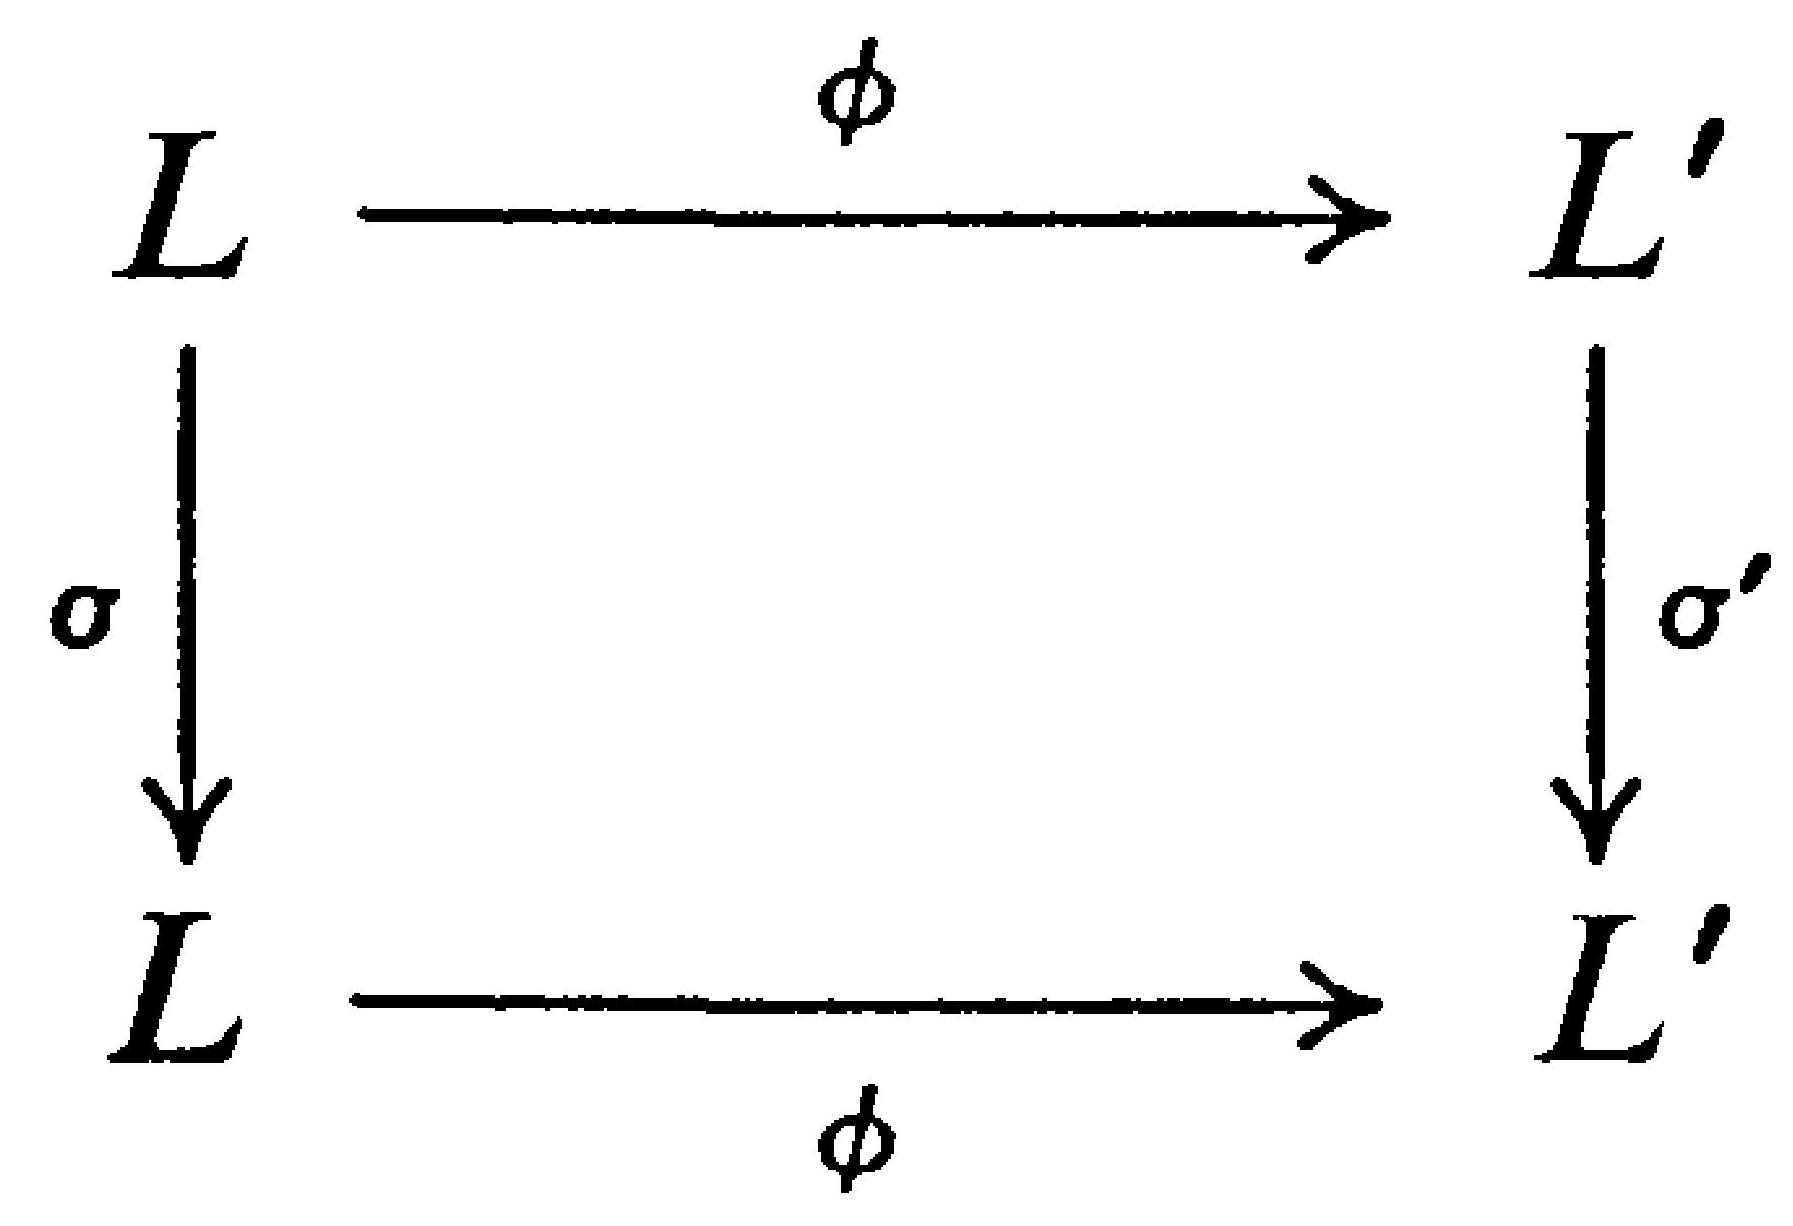
\includegraphics[max width=\textwidth, center]{2025_06_06_fac2836a92464059da43g-095}

Proof. It suffices to prove this in case $\sigma^{\prime}=\exp \operatorname{ad}_{L^{\prime}} x^{\prime}, x^{\prime} \in \mathscr{N}\left(L^{\prime}\right)$. By the preceding remark, $x^{\prime}=\phi(x)$ for at least one $x \in \mathscr{N}(L)$. For arbitrary $z \in L,\left(\phi \circ \exp \operatorname{ad}_{L} x\right)(z)=\phi(z+[x z]+(1 / 2)[x[x z]]+\ldots)=\phi(z)+\left[x^{\prime} \phi(z)\right]+$ $\left.(1 / 2)\left[x^{\prime}\left[x^{\prime} \phi(z)\right]\right]+\ldots\right)=\left(\exp \operatorname{ad}_{L^{\prime}} x^{\prime} \circ \phi\right)(z)$. In other words, the diagram commutes.

\subsection*{16.2. Conjugacy of CSA's (solvable case)}
Theorem. Let $L$ be solvable, $\mathscr{E}(L)$ as in (16.1). Then any two CSA's $H_{1}, H_{2}$ of $L$ are conjugate under $\mathscr{E}(L)$.

Proof. Use induction on $\operatorname{dim} L$, the case $\operatorname{dim} L=1$ (or $L$ nilpotent) being trivial. Assume that $L$ is not nilpotent. Since $L$ is solvable, $L$ possesses non-\\
zero abelian ideals (e.g., the last nonzero term of the derived series); choose $A$ to be one of smallest possible dimension. Set $L^{\prime}=L / A$, and denote the canonical map $\phi: L \rightarrow L / A$ by $x \mapsto x^{\prime}$. According to Lemma A of (15.4), $H_{1}^{\prime}$ and $H_{2}^{\prime}$ are CSA's of the (solvable) algebra $L^{\prime}$. By induction, there exists $\sigma^{\prime} \in \mathscr{E}\left(L^{\prime}\right)$ sending $H_{1}^{\prime}$ onto $H_{2}^{\prime}$. Then Lemma 16.1 allows us to find $\sigma \in \mathscr{E}(L)$ such that the diagram there commutes. This means that $\sigma$ maps the full inverse image $K_{1}=\phi^{-1}\left(H_{1}^{\prime}\right)$ onto $K_{2}=\phi^{-1}\left(H_{2}^{\prime}\right)$. But now $H_{2}$ and $\sigma\left(H_{1}\right)$ are both CSA's of the algebra $K_{2}$. If $K_{2}$ is smaller than $L$, induction allows us to find $\tau^{\prime} \in \mathscr{E}\left(K_{2}\right)$ such that $\tau^{\prime} \sigma\left(H_{1}\right)=H_{2}$; but $\mathscr{E}\left(K_{2}\right)$ consists of the restrictions to $K_{2}$ of the elements of $\mathscr{E}\left(L ; K_{2}\right) \subset \mathscr{E}(L)$, so this says that $\tau \sigma\left(H_{1}\right)=$ $H_{2}$ for $\tau \in \mathscr{E}(L)$ whose restriction to $K_{2}$ is $\tau^{\prime}$, and we're done.

Otherwise we must have $L=K_{2}=\sigma\left(K_{1}\right)$, so in fact $K_{1}=K_{2}$ and $L=$ $H_{2}+A=H_{1}+A$. To settle this case, we must explicitly construct an automorphism of $L$ (this is the only point in the whole argument where we have to do so!). The CSA $H_{2}$ is of the form $L_{0}(\operatorname{ad} x)$ for suitable $x \in L$, thanks to Theorem 15.3. $A$ being ad $x$ stable, $A=A_{0}(\operatorname{ad} x) \oplus A_{*}(\operatorname{ad} x)(\operatorname{cf.}(15.1))$, and each summand is stable under $L=H_{2}+A$. By the minimality of $A$, we have either $A=A_{0}(\operatorname{ad} x)$ or else $A=A_{*}(\operatorname{ad} x)$. The first case is absurd, since it would force $A \subset H_{2}, L=H_{2}$, contrary to the assumption that $L$ is not nilpotent. So $A=A_{*}(\operatorname{ad} x)$, whence (clearly) $A=L_{*}(\operatorname{ad} x)$.

Since $L=H_{1}+A$, we can now express $x=y+z$, where $y \in H_{1}, z \in L_{*}$ (ad $x$ ). In turn, write $z=\left[x z^{\prime}\right], z^{\prime} \in L_{*}(\operatorname{ad} x)$, using the fact that ad $x$ is invertible on $L_{*}(\operatorname{ad} x)$. Since $A$ is abelian, $\left(\operatorname{ad} z^{\prime}\right)^{2}=0$, so exp ad $z^{\prime}=1_{L}$ $+\mathrm{ad} z^{\prime}$; applied to $x$, this yields $x-z=y$. In particular, $H=L_{0}(\operatorname{ad} y)$ must also be a CSA of $L$. Since $y \in H_{1}, H \supset H_{1}$, whence $H=H_{1}$ (both being minimal Engel). So $H_{1}$ is conjugate to $H_{2}$ via exp ad $z^{\prime}$.

It remains only to observe that exp ad $z^{\prime}$ does lie in $\mathscr{E}(L): z^{\prime}$ can be written as sum of certain strongly ad-nilpotent elements $z_{i}$ of $A=L_{*}(\operatorname{ad} x)$, but the latter "commute" ( $A$ is abelian), so exp ad $z^{\prime}=\prod_{i} \exp$ ad $z_{i} \in \mathscr{E}(L)$. $\square$

\subsection*{16.3. Borel subalgebras}
To pass from the solvable case to the general case, we utilize Borel subalgebras of a Lie algebra $L$, which are by definition the maximal solvable subalgebras of $L$. If we can show that any two Borel subalgebras of $L$ are conjugate under $\mathscr{E}(L)$, then it will follow from Theorem 16.2 that all CSA's of $L$ are conjugate.

Lemma A. If $B$ is a Borel subalgebra of $L$, then $B=N_{L}(B)$.\\
Proof. Let $x$ normalize $B$. Then $B+\mathrm{F} x$ is a subalgebra of $L$, solvable because $[B+\mathrm{F} x, B+\mathrm{F} x] \subset B$, whence $x \in B$ by maximality of $B$.

Lemma B. If Rad $L \neq L$, then the Borel subalgebras of $L$ are in natural 1-1 correspondence with those of the semisimple Lie algebra L/Rad L.

Proof. Rad $L$ being a solvable ideal of $L, B+\operatorname{Rad} L$ is a solvable subalgebra of $L$ for any Borel subalgebra $B$ of $L$, i.e., Rad $L \subset B$ (by maximality). The lemma follows at once.

From Lemma B it follows that the essential case is that in which $L$ is semisimple. In this situation, let $H$ be a CSA, $\Phi$ the root system of $L$ relative to $H$. Fix a base $\Delta$, and with it a set of positive roots. Set $B(\Delta)=H+\coprod_{\alpha \succ 0} L_{\alpha}$, $N(\Delta)=\coprod_{\alpha \succ 0} L_{\alpha}$. Then we know that $B(\Delta)$ is a subalgebra of $L$, with derived algebra $N(\Delta)$. Furthermore, $N(\Delta)$ is nilpotent: If $x \in L_{\alpha}(\alpha \succ 0)$, then application of ad $x$ to root vectors for roots of positive height (relative to $\Delta$ ) increases height by at least one; this shows how to make the descending central series go to zero. It follows now that $B(\Delta)$ is solvable. In fact, we claim that $B(\Delta)$ is a Borel subalgebra: Indeed, let $K$ be any subalgebra of $L$ properly including $B(\Delta)$. Then $K$, being stable under ad $H$, must include some $L_{\alpha}$ for $\alpha \prec 0$. But this forces $K$ to include the simple algebra $S_{\alpha}$; in particular, $K$ cannot be solvable.

Lemma C. Let $L$ be semisimple, with CSA $H$ and root system $\Phi$. For each base $\Delta \subset \Phi, B(\Delta)$ is a Borel subalgebra of $L$ (called standard relative to $H$ ). All standard Borel subalgebras of $L$ relative to $H$ are conjugate under $\mathscr{E}(L)$.

Proof. Only the second statement remains to be proved. Recall (14.3) that the reflection $\sigma_{\alpha}$, acting on $H$, may be extended to an inner automorphism $\tau_{\alpha}$ of $L$, which is (by construction) in $\mathscr{E}(L)$. It is clear that this automorphism sends $B(\Delta)$ to $B\left(\sigma_{\alpha} \Delta\right)$. Using the fact that the Weyl group is generated by reflections and acts transitively on bases, we see that $\mathscr{E}(L)$ acts transitively on the standard Borels relative to $H$.

\subsection*{16.4. Conjugacy of Borel subalgebras}
Theorem. The Borel subalgebras of an arbitrary Lie algebra $L$ are all conjugate under $\mathscr{E}(L)$.

Corollary. The Cartan subalgebras of an arbitrary Lie algebra $L$ are conjugate under $\mathscr{E}(L)$.

Proof of Corollary. Let $H, H^{\prime}$ be two CSA's of $L$. Being nilpotent (hence solvable), each lies in at least one Borel subalgebra, say $B$ and $B^{\prime}$ (respectively). By the theorem, there exists $\sigma \in \mathscr{E}(L)$ such that $\sigma(B)=B^{\prime}$. Now $\sigma(H)$ and $H^{\prime}$ are both CSA's of the solvable algebra $B^{\prime}$, so by Theorem 16.2 there exists $\tau^{\prime} \in \mathscr{E}\left(B^{\prime}\right)$ for which $\tau^{\prime} \sigma(H)=H^{\prime}$. But $\tau^{\prime}$ is the restriction to $B^{\prime}$ of some $\tau \in \mathscr{E}\left(L ; B^{\prime}\right) \subset \mathscr{E}(L)(16.1)$, so finally $\tau \sigma(H)=H^{\prime} . \tau \sigma \in \mathscr{E}(L)$.

Proof of Theorem. We proceed by induction on $\operatorname{dim} L$, the case $\operatorname{dim} L=$ 1 being trivial. By Lemmas 16.1 and 16.3 B , along with the induction hypothesis, we may assume that $L$ is semisimple. Fix a standard Borel subalgebra $B$ (relative to some CSA). It will suffice to show that any other Borel subalgebra $B^{\prime}$ is conjugate to $B$ under $\mathscr{E}(L)$. If $B \cap B^{\prime}=B$, there is nothing to prove (since this forces $B^{\prime}=B$ by maximality). Therefore, we may also use a second (downward) induction on $\operatorname{dim}\left(B \cap B^{\prime}\right)$ : by assumption, any Borel subalgebra whose intersection with $B$ (or a conjugate of $B$ ) has larger dimension is already conjugate to $B$.\\
(1) First suppose that $B \cap B^{\prime} \neq 0$. Two cases arise:

Case (i): The set $N^{\prime}$ of nilpotent elements of $B \cap B^{\prime}$ is nonzero. Since $B$ is standard, $N^{\prime}$ is a subspace and the derived algebra of $B \cap B^{\prime}$ consists of nilpotent elements. This implies in turn that $N^{\prime}$ is an ideal in $B \cap B^{\prime} . N^{\prime}$ is of course not an ideal of $L$, so its normalizer $K$ is a proper subalgebra of $L$.

Next we show that $B \cap B^{\prime}$ is properly contained in both $B \cap K, B^{\prime} \cap K$. For consider the action of $N^{\prime}$ on $B /\left(B \cap B^{\prime}\right)$ induced by ad. Each $x \in N^{\prime}$ acts nilpotently on this vector space, so by Theorem 3.3 there must exist nonzero $y+\left(B \cap B^{\prime}\right)$ killed by all $x \in N^{\prime}$, i.e., such that $[x y] \in B \cap B^{\prime}, y \notin B \cap B^{\prime}$. But $[x y]$ is also in $[B B]$, so is nilpotent; this forces $[x y] \in N^{\prime}$, or $y \in N_{B}\left(N^{\prime}\right)=$ $B \cap K$, while $y \notin B \cap B^{\prime}$. Similarly, $B \cap B^{\prime}$ is properly contained in $B^{\prime} \cap K$.

On the other hand, $B \cap K$ and $B^{\prime} \cap K$ are solvable subalgebras of $K$. Let $C, C^{\prime}$ be respective Borel subalgebras of $K$ including them (Figure 1). Since $K \neq L$, induction yields $\sigma \in \mathscr{E}(L ; K) \subset \mathscr{E}(L)$ such that $\sigma\left(C^{\prime}\right)=C$. Because $B \cap B^{\prime}$ is a proper (nonzero) subalgebra of both $C$ and $C^{\prime}$, the second induction hypothesis then yields $\tau \in \mathscr{E}(L)$ such that $\tau \sigma\left(C^{\prime}\right) \subset B$ (i.e., $\tau$ sends a Borel subalgebra of $L$ including $\sigma\left(C^{\prime}\right)=C$ onto $B$ ). Finally,\\
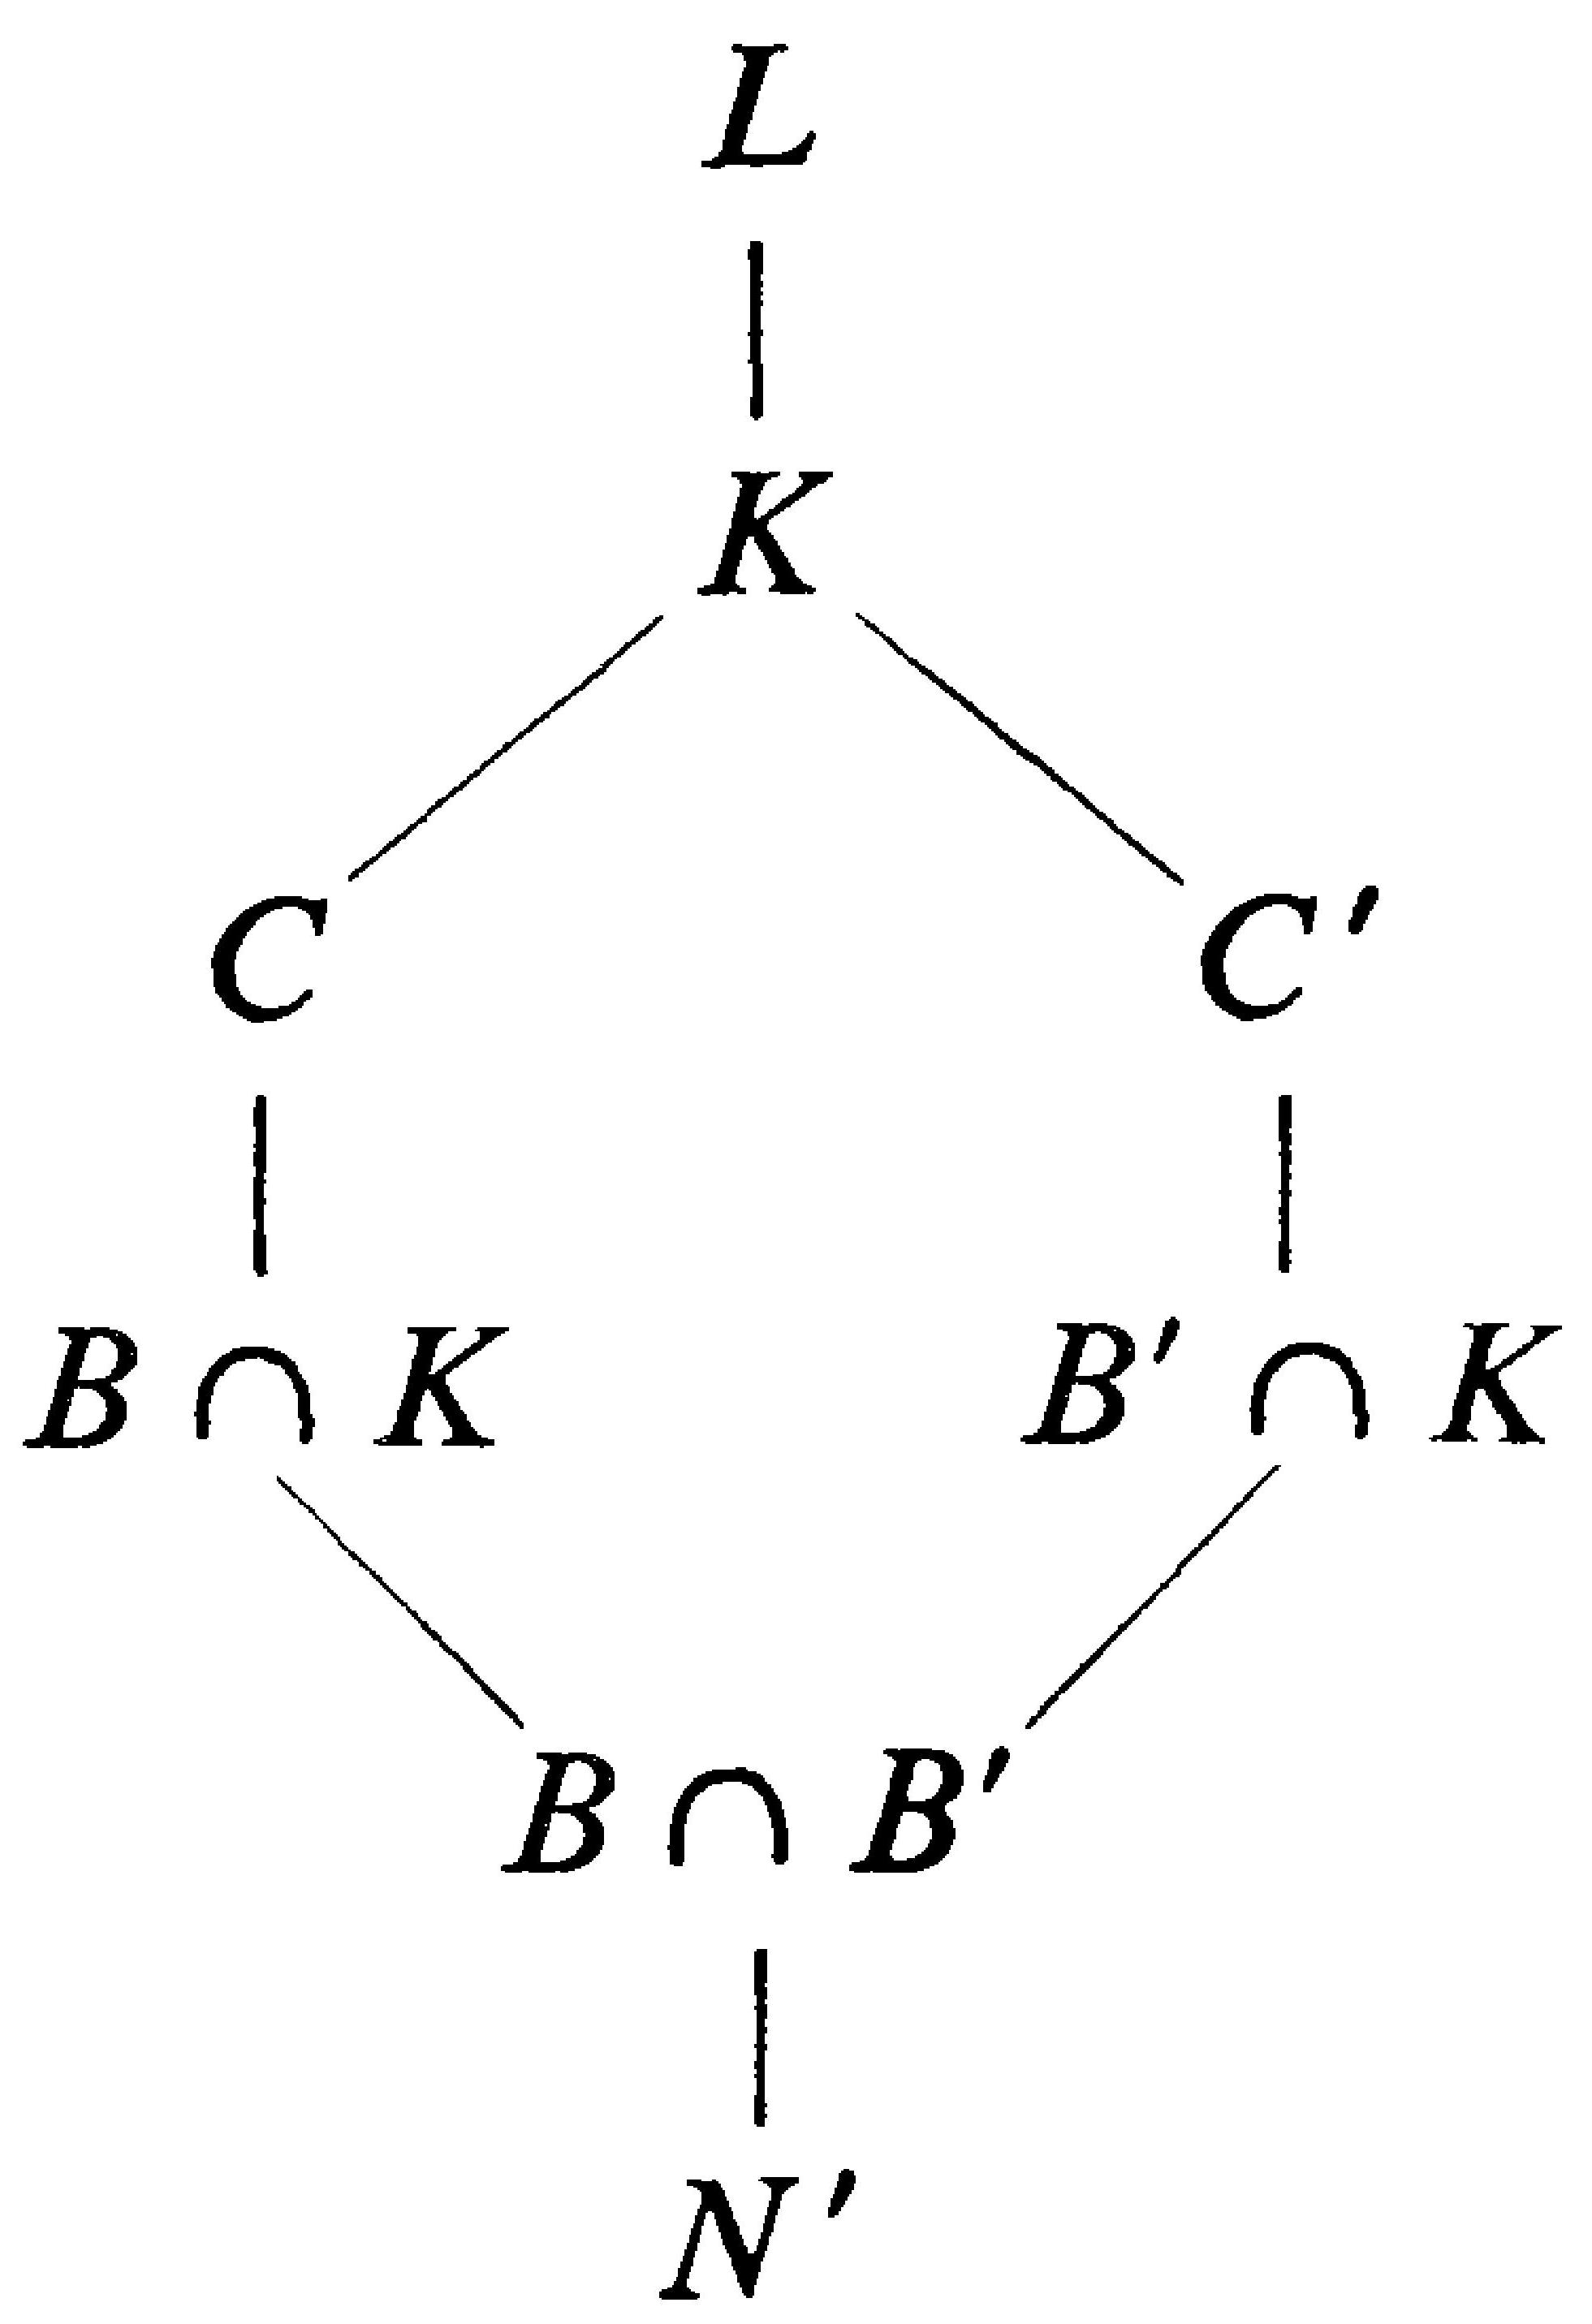
\includegraphics[max width=\textwidth, center]{2025_06_06_fac2836a92464059da43g-098}

Figure 1\\
$B \cap \tau \sigma\left(B^{\prime}\right) \supset \tau \sigma\left(C^{\prime}\right) \cap \tau \sigma\left(B^{\prime}\right) \supset \tau \sigma\left(B^{\prime} \cap K\right) \supsetneqq \tau \sigma\left(B \cap B^{\prime}\right)$, so the former has greater dimension than $B \cap B^{\prime}$. Again appealing to the second induction hypothesis, we see that $B$ is conjugate under $\mathscr{E}(L)$ to $\tau \sigma\left(B^{\prime}\right)$, and we're done with case (i).

Case (ii): $B \cap B^{\prime}$ has no nonzero nilpotent elements. Note that any Borel subalgebra of $L$ contains the semisimple and nilpotent parts of its elements, thanks to Proposition 4.2(c) and Lemma 16.3A. This shows at once that $B \cap B^{\prime}=T$ is a toral subalgebra. Now we use the fact that $B$ is a standard Borel subalgebra, say $B=B(\Delta), N=N(\Delta), B=H+N$. Since $[B B]=N$, and since $T \cap N=0$, it is clear that $N_{B}(T)=C_{B}(T)$. Let $C$ be any CSA of $C_{B}(T)$; in particular, $C$ is nilpotent and $T \subset N_{C_{B}(T)}(C)=C$. If $n \in N_{B}(C), t \in T \subset C$, then $(\operatorname{ad} t)^{k} n=0$ for some $k$ since $C$ is nilpotent. But ad $t$ is semisimple, so $k=1$ and $n \in C_{B}(T)$. Thus $N_{B}(C)=N_{C_{B}(T)}(C)=C$. As a nilpotent self-normalizing subalgebra of $B, C$ is therefore a CSA of $B$\\
(which includes $T$ ). We know, thanks to Theorem 16.2, that $C$ is a maximal toral subalgebra of $L$ conjugate under $\mathscr{E}(B)$ (hence under $\mathscr{E}(L)$ ) to $H$, so without loss of generality we may now assume that $T \subset H$.

Suppose $T=H$. Evidently $B^{\prime} \supsetneqq H$, so $B^{\prime}$ must include at least one $L_{\alpha}$ ( $\alpha \prec 0$ relative to $\Delta$ ). Applying $\tau_{\alpha}$ (cf. Lemma C of 16.3) to $B^{\prime}$ yields a Borel subalgebra $B^{\prime \prime}$ whose intersection with $B$ includes $H+L_{-\alpha}$; so the second induction hypothesis shows that $B^{\prime \prime}$ is conjugate in turn to $B$, and we're done.

Next suppose $T$ is properly included in $H$. Now either $B^{\prime}$ centralizes $T$ or not. If $B^{\prime} \subset C_{L}(T)$, then we can appeal to the first induction hypothesis, since $\operatorname{dim} C_{L}(T)<\operatorname{dim} L(T \neq 0$ and $Z(L)=0)$. Namely, use the fact that $H \subset C_{L}(T)$ to find a Borel subalgebra $B^{\prime \prime}$ of $C_{L}(T)$ including $H$, then use induction to find $\sigma \in \mathscr{E}\left(L ; C_{L}(T)\right) \subset \mathscr{E}(L)$ sending $B^{\prime}$ onto $B^{\prime \prime}$. In particular, $B^{\prime \prime}$ is a Borel subalgebra of $L$, including $H$, so it is conjugate to $B$ under $\mathscr{E}(L)$ because of the second induction hypothesis.

We are left with the situation $B^{\prime} \nsubseteq C_{L}(T)$. This allows us to find a common eigenvector $x \in B^{\prime}$ for ad $T$, and an element $t \in T$ for which $[t x]=a x$, with a rational and positive. Define $S=H+\amalg L_{\alpha}, \alpha \in \Phi$ running over those roots for which $\alpha(t)$ is rational and positive. It is clear that $S$ is a subalgebra of $L$ (and $x \in S$ ). Moreover, it is immediate that $S$ is solvable (cf. proof of Lemma 16.3C). Let $B^{\prime \prime}$ be a Borel subalgebra of $L$ which includes $S$. Now $B^{\prime \prime} \cap B^{\prime} \supset T+\mathrm{F} x \supsetneqq T=B^{\prime} \cap B$, so $\operatorname{dim} B^{\prime \prime} \cap B^{\prime}>\operatorname{dim} B \cap B^{\prime}$. Similarly, $B^{\prime \prime} \cap B \supset H \supsetneqq T$, so $\operatorname{dim} B^{\prime \prime} \cap B>\operatorname{dim} B^{\prime} \cap B$. The second induction hypothesis, applied to this last inequality, shows that $B^{\prime \prime}$ is conjugate to $B$. (In particular, $B^{\prime \prime}$ is obviously standard relative to a CSA conjugate to $H$.) The second induction hypothesis next applies (because $B^{\prime \prime}$ is standard) to the first inequality, showing that $B^{\prime \prime}$ is conjugate to $B^{\prime}$. So $B$ is conjugate to $B^{\prime}$.\\
(2) This disposes of all cases for which $B \cap B^{\prime} \neq 0$. Consider now what happens if $B \cap B^{\prime}=0$. This forces $\operatorname{dim} L \geq \operatorname{dim} B+\operatorname{dim} B^{\prime}$; since $B$ is standard, we know $\operatorname{dim} B>(1 / 2) \operatorname{dim} L$, so $B^{\prime}$ must be "too small". More precisely, take $T$ to be a maximal toral subalgebra of $B^{\prime}$. If $T=0$, then $B^{\prime}$ consists of nilpotent elements; $B^{\prime}$ is therefore nilpotent (Engel's Theorem) as well as self-normalizing (Lemma A of (16.3)), i.e., $B^{\prime}$ is a CSA. But this is absurd, since we know (Corollary 15.3) that all CSA's of $L$ are toral. Therefore $T \neq 0$. If $H_{0}$ is a maximal toral subalgebra of $L$ including $T$, then $B^{\prime}$ has nonzero intersection with any standard Borel subalgebra $B^{\prime \prime}$ relative to $H_{0}$. Therefore $B^{\prime}$ is conjugate to $B^{\prime \prime}$, by the first part of the proof, so dim $B^{\prime}=\operatorname{dim} B^{\prime \prime}>(1 / 2) \operatorname{dim} L$, contradicting the "smallness" of $B^{\prime}$. $\square$

Corollary 16.4 allows us to attach a numerical invariant (called rank) to an arbitrary Lie algebra $L$ over F, namely, the dimension of a CSA of $L$. In case $L$ is semisimple, rank $L$ coincides with rank $\Phi, \Phi$ the root system of $L$ relative to any maximal toral subalgebra ( $=$ CSA) .

It is worthwhile to note one byproduct of the conjugacy theorem for Borel subalgebras. Let $L$ be semisimple, with CSA $H$ and root system $\Phi$. We claim that any Borel subalgebra $B$ of $L$ which includes $H$ is standard. Indeed, let $\sigma(B(\Delta))=B$, where $\Delta$ is some given base of $\Phi, \sigma \in \mathscr{E}(L)$. Since\\
$H$ and $\sigma(H)$ are two CSA's of $B$, they are conjugate under $\mathscr{E}(L ; B) \subset \mathscr{E}(L)$ (Theorem 16.2), so we may as well assume that $\sigma(H)=H$. Then it is clear that for each $\alpha>0, \sigma\left(L_{\alpha}\right)=L_{\sigma \alpha}$, with $\sigma \alpha$ a root. Moreover, the permutation of roots effected by $\sigma$ preserves sums, so $\sigma(\Delta)=\Delta^{\prime}$ is again a base of $\Phi$ and $B=B\left(\Delta^{\prime}\right)$ is standard.

\subsection*{16.5. Automorphism groups}
Let $L$ be semisimple, $H$ a CSA of $L$, with root system $\Phi$ and some fixed base $\Delta$. If $\tau$ is any automorphism of $L$, then of course $\tau(B), B=B(\Delta)$, is another Borel subalgebra of $L$, so it is sent back to $B$ by some $\sigma_{1} \in \mathscr{E}(L)$ (Theorem 16.4). Now $H$ and $\sigma_{1} \tau(H)$ are two CSA's of $L$ (hence also CSA's of $B$ ), so we can find $\sigma_{2} \in \mathscr{E}(L ; B) \subset \mathscr{E}(L)$ which sends $\sigma_{1} \tau(H)$ to $H$ (and leaves $B$ invariant), thanks to Theorem 16.2. Since $\sigma_{2} \sigma_{1} \tau$ simultaneously preserves $H$ and $B$, it induces an automorphism of $\Phi$ which leaves $\Delta$ invariant. From (12.2) we know all such automorphisms: the nontrivial ones arise from nontrivial graph automorphisms, which exist (for $\Phi$ irreducible) only in the cases $\mathrm{A}_{\ell}(\ell>1), \mathrm{D}_{\ell}, \mathrm{E}_{6}$. Let $\rho$ be a corresponding automorphism of $L$ (cf. Exercise 14.6). Because $\rho$ is not quite unique, we may adjust the scalars involved in such a way that $\rho \sigma_{2} \sigma_{1} \tau$ sends $x_{\alpha}$ to $c_{\alpha} x_{\alpha}(\alpha>0), y_{\alpha}$ to $c_{\alpha}^{-1} y_{\alpha}$, hence $h_{\alpha}$ to $h_{\alpha}$ (hence all $h$ to themselves). The upshot is that $\tau$ differs from an element of the group $\mathscr{E}(L) \cdot \Gamma(L), \Gamma(L)=$ group of graph automorphisms of $L$, only by a diagonal automorphism, i.e., an automorphism which is the identity on $H$ and scalar multiplication on each root space $L_{\alpha}$.

It can be proved (see Jacobson [1], p. 278) that a diagonal automorphism is always inner; in fact, the construction shows that it can be found in $\mathscr{E}(L)$. Moreover, the product Aut $L=\operatorname{Int}(L) \cdot \Gamma(L)$ turns out to be semidirect (Jacobson [1], Chapter IX, exercises), so in particular $\mathscr{E}(L)=\operatorname{Int}(L)$. The reader will also find in Jacobson's book detailed descriptions of the automorphism groups for various simple Lie algebras.

\section*{Exercises}
\begin{enumerate}
  \item Prove that $\mathscr{E}(L)$ has order one if and only if $L$ is nilpotent.
  \item Let $L$ be semisimple, $H$ a CSA, $\Delta$ a base of $\Phi$. Prove that any subalgebra of $L$ consisting of nilpotent elements, and maximal with respect to this property, is conjugate under $\mathscr{E}(L)$ to $N(\Delta)$, the derived algebra of $B(\Delta)$.
  \item Let $\Psi$ be a set of roots which is closed ( $\alpha, \beta \in \Psi, \alpha+\beta \in \Phi$ implies $\alpha+\beta \in \Psi$ ) and satisfies $\Psi \cap-\Psi=\varnothing$. Prove that $\Psi$ is included in the set of positive roots relative to some base of $\Phi$. [Use Exercise 2.] (This exercise belongs to the theory of root systems, but is easier to do using Lie algebras.)
  \item How does the proof of Theorem 16.4 simplify in case $L=\mathfrak{s l}(2, \mathrm{~F})$ ?
  \item Let $L$ be semisimple. If a semisimple element of $L$ is regular, then it lies in only finitely many Borel subalgebras. (The converse is also true, but harder to prove, and suggests a notion of "regular" for elements of $L$ which are not necessarily semisimple.)
  \item Let $L$ be semisimple, $L=H+\amalg L_{\alpha}$. A subalgebra $P$ of $L$ is called\\
parabolic if $P$ includes some Borel subalgebra. (In that case $P$ is selfnormalizing, by Lemma 15.2B.) Fix a base $\Delta \subset \Phi$, and set $B=B(\Delta)$. For each subset $\Delta^{\prime} \subset \Delta$, define $P\left(\Delta^{\prime}\right)$ to be the subalgebra of $L$ generated by all $L_{\alpha}\left(\alpha \in \Delta\right.$ or $\left.-\alpha \in \Delta^{\prime}\right)$, along with $H$.\\
(a) $P\left(\Delta^{\prime}\right)$ is a parabolic subalgebra of $L$ (called standard relative to $\Delta$ ).\\
(b) Each parabolic subalgebra of $L$ including $B(\Delta)$ has the form $P\left(\Delta^{\prime}\right)$ for some $\Delta^{\prime} \subset \Delta$. [Use the Corollary of Lemma 10.2A and Proposition 8.4(d).]\\
(c) Prove that every parabolic subalgebra of $L$ is conjugate under $\mathscr{E}(L)$ to one of the $P\left(\Delta^{\prime}\right)$.
  \item Let $L=\mathfrak{s l}(2, \mathrm{~F})$, with standard basis $(x, h, y)$. For $c \in \mathrm{~F}$, write $x(c)=$ $\exp \operatorname{ad}(c x), y(c)=\exp \operatorname{ad}(c y)$. Define inner automorphisms $w(c)=$ $x(c) y\left(-c^{-1}\right) x(c), h(c)=w(c) w(1)^{-1}(=w(c) w(-1))$, for $c \neq 0$. Compute the matrices of $w(c), h(c)$ relative to the given basis of $L$, and deduce that all diagonal automorphisms (16.5) of $L$ are inner. Conclude in this case that Aut $L=\operatorname{Int} L=\mathscr{E}(L)$.
  \item Let $L$ be semisimple. Prove that the intersection of two Borel subalgebras $B, B^{\prime}$ of $L$ always includes a CSA of $L$. [The proof is not easy; here is one possible outline:\\
(a) Let $N, N^{\prime}$ be the respective ideals of nilpotent elements in $B, B^{\prime}$. Relative to the Killing form of $L, N=B^{\perp}, N^{\prime}=B^{\prime \perp}$, where $\perp$ denotes orthogonal complement.\\
(b) Therefore $B=N^{\perp}=\left(N+\left(N \cap N^{\prime}\right)\right)^{\perp}=\left(N+\left(B \cap N^{\prime}\right)\right)^{\perp}=N^{\perp} \cap$ $\left(B^{\perp}+N^{\prime \perp}\right)=B \cap\left(N+B^{\prime}\right)=N+\left(B \cap B^{\prime}\right)$.\\
(c) Note that $A=B \cap B^{\prime}$ contains the semisimple and nilpotent parts of its elements.\\
(d) Let $T$ be a maximal toral subalgebra of $A$, and find a $T$-stable complement $A^{\prime}$ to $A \cap N$. Then $A^{\prime}$ consists of semisimple elements. Since $B / N$ is abelian, $\left[T A^{\prime}\right]=0$, forcing $A^{\prime}=T$.\\
(e) Combine (b), (d) to obtain $B=N+T$; thus $T$ is a maximal toral subalgebra of L.]
\end{enumerate}

\section*{Notes}
The proof of Theorem 16.4 is due to Winter [1] (inspired in part by G. D. Mostow); see also Barnes [1]. Most of the older proofs use analytic methods ( $F=\mathbf{C}$ ) or else some algebraic geometry: see Bourbaki [3], Chap. VII, Chevalley [2], Jacobson [1], Séminaire "Sophus Lie" [1], Serre [2]. For detailed accounts of the automorphism groups, consult Jacobson [1], Seligman [1].

\section*{Chapter V}
\section*{Existence Theorem}
\section*{17. Universal enveloping algebras}
In this section F may be an arbitrary field (except where otherwise noted). We shall associate to each Lie algebra $L$ over $F$ an associative algebra with 1 (infinite dimensional, in general), which is generated as "freely" as possible by $L$ subject to the commutation relations in $L$. This "universal enveloping algebra" is a basic tool in representation theory. Although it could have been introduced right away in Chapter I, we deferred it until now in order to avoid the unpleasant task of proving the Poincaré-Birkhoff-Witt Theorem before it was really needed. The reader is advised to forget temporarily all the specialized theory of semisimple Lie algebras.

\subsection*{17.1. Tensor and symmetric algebras}
First we introduce a couple of algebras defined by universal properties. (For further details consult, e.g., S. Lang, Algebra, Reading, Mass.: Addison-Wesley 1965, Ch. XVI.) Fix a finite dimensional vector space $V$ over F. Let $T^{0} V=\mathrm{F}, T^{1} V=V, T^{2} V=V \otimes V, \ldots, T^{m} V=V \otimes \ldots \otimes$ $V$ ( $m$ copies). Define $\mathfrak{I}(V)=\coprod_{i=0}^{\infty} T^{i} V$, and introduce an associative product, defined on homogeneous generators of $\mathfrak{I}(V)$ by the obvious rule ( $v_{1} \otimes \ldots$ $\left.\otimes v_{k}\right)\left(w_{1} \otimes \ldots \otimes w_{m}\right)=v_{1} \otimes \ldots \otimes v_{k} \otimes w_{1} \otimes \ldots \otimes w_{m} \in T^{k+m} V$. This makes $\mathfrak{I}(V)$ an associative graded algebra with 1 , which is generated by 1 along with any basis of $V$. We call it the tensor algebra on $V$. $\mathfrak{I}(V)$ is the universal associative algebra on $n$ generators ( $n=\operatorname{dim} V$ ), in the following sense: given any F-linear map $\phi: V \rightarrow \mathfrak{A}$ ( $\mathfrak{A}$ an associative algebra with 1 over $F$ ), there exists a unique homomorphism of F-algebras $\psi: \mathfrak{I}(V) \rightarrow \mathfrak{A}$ such that $\psi(1)=1$ and the following diagram commutes ( $i=$ inclusion):\\
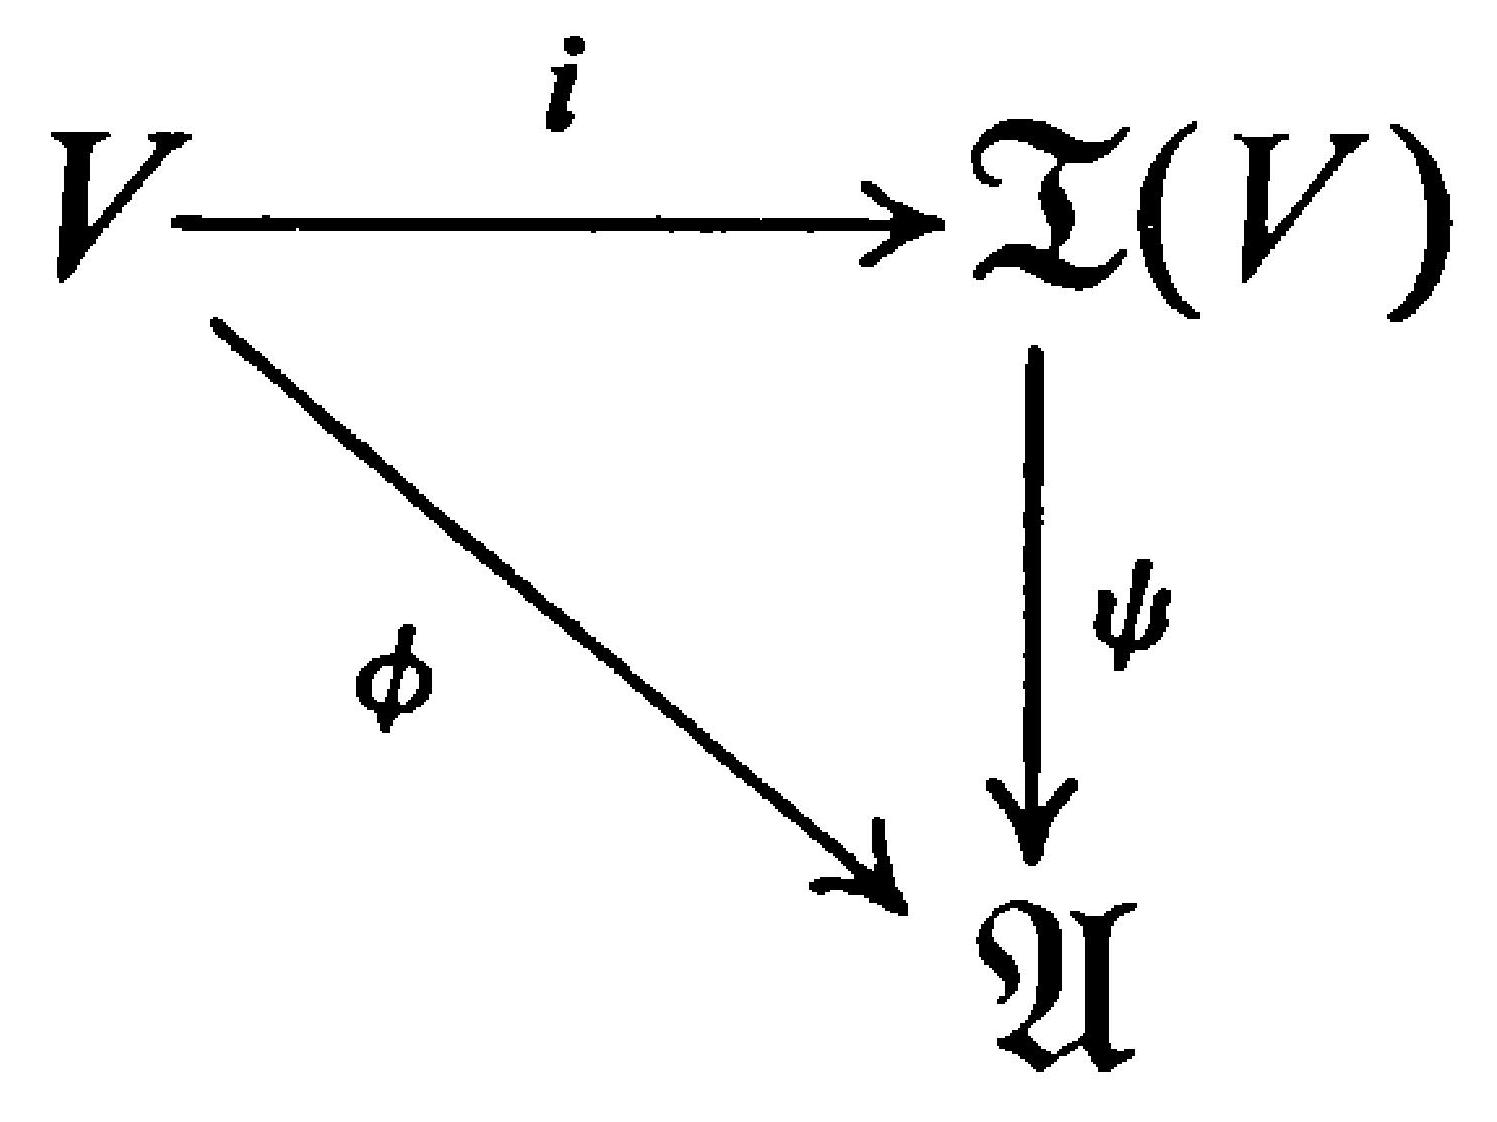
\includegraphics[max width=\textwidth, center]{2025_06_06_fac2836a92464059da43g-102}

Next let $I$ be the (two sided) ideal in $\mathfrak{T}(V)$ generated by all $x \otimes y-y \otimes x$ $(x, y \in V)$ and call $\mathfrak{G}(V)=\mathfrak{I}(V) / I$ the symmetric algebra on $V ; \sigma: \mathfrak{I}(V) \rightarrow$ $\mathfrak{S}(V)$ will denote the canonical map. Notice that the generators of $I$ lie in $T^{2} V$; this makes it obvious that $I=\left(I \cap T^{2} V\right) \oplus\left(I \cap T^{3} V\right) \oplus \ldots$. Therefore, $\sigma$ is injective on $T^{0} V=\mathrm{F}, T^{1} V=V$ (allowing us to identify $V$ with a subspace of $\mathfrak{S}(V)$ ), and $\mathfrak{S}(V)$ inherits a grading from $\mathfrak{I}(V): \mathfrak{S}(V)$\\
$=\coprod_{i=0}^{\infty} S^{i} V$. The effect of factoring out $I$ is just to make the elements of $V$ commute; so $\mathfrak{G}(V)$ is universal (in the above sense) for linear maps of $V$ into commutative associative F -algebras with 1 . Moreover, if $\left(x_{1}, \ldots, x_{n}\right)$ is any fixed basis of $V$, then $\mathfrak{S}(V)$ is canonically isomorphic to the polynomial algebra over F in $n$ variables, with basis consisting of 1 and all $x_{i(1)} \ldots x_{i(t)}, t \geq 1,1 \leq i(1) \leq \ldots \leq i(t) \leq n$.

The reader can easily verify that the preceding constructions go through even when $V$ is infinite dimensional.

For use much later (in §23) we mention a special fact in case char $\mathrm{F}=0$. The symmetric group $\mathscr{S}_{m}$ acts on $T^{m} V$ by permuting subscripts of tensors $v_{1} \otimes \ldots \otimes v_{m}\left(v_{i} \in V\right)$. An element of $T^{m} V$ fixed by $\mathscr{S}_{m}$ is called a homogeneous symmetric tensor of order m. Example: $x \otimes y+y \otimes x$ (order 2). Fix a basis $\left(x_{1}, \ldots, x_{n}\right)$ of $V$, so the products $x_{i(1)} \otimes \ldots \otimes x_{i(m)}(1 \leq i(j)$ $\leq n$ ) form a basis of $T^{m} V$. For each ordered sequence $1 \leq i(1) \leq i(2) \ldots$ $\leq i(m) \leq n$, define a symmetric tensor


\begin{equation*}
\frac{1}{m!} \sum_{\pi \in \mathscr{S}_{m}} x_{i(\pi(1))} \otimes \ldots \otimes x_{i(\pi(m))} \tag{*}
\end{equation*}


(which makes sense since $m!\neq 0$ in F). The images of these tensors in $S^{m} V$ are nonzero and clearly form a basis there, so the tensors (\textit{) in turn must span a complement to $I \cap T^{m} V$ in $T^{m} V$. On the other hand, the tensors (}) obviously span the space of all symmetric tensors of order $m$ (call it $\tilde{S}^{m} V \subset$ $\left.T^{m} V\right)$. We conclude that $\sigma$ defines a vector space isomorphism of $\widetilde{S}^{m} V$ onto $S^{m} V$, hence of the space $\widetilde{\mathfrak{S}}(V)$ of all symmetric tensors onto $\mathfrak{S}(V)$.

\subsection*{17.2. Construction of $\mathfrak{U}(L)$}
We begin with the abstract definition, for an arbitrary Lie algebra $L$ (allowed here to be infinite dimensional, contrary to our usual convention). A universal enveloping algebra of $L$ is a pair ( $\mathfrak{U}, i$ ), where $\mathfrak{U}$ is an associative algebra with 1 over $\mathrm{F}, i: L \rightarrow \mathfrak{U}$ is a linear map satisfying


\begin{equation*}
i([x y])=i(x) i(y)-i(y) i(x) \tag{*}
\end{equation*}


for $x, y \in L$, and the following holds: for any associative F-algebra $\mathfrak{A}$ with 1 and any linear map $j: L \rightarrow \mathfrak{A}$ satisfying (*), there exists a unique homomorphism of algebras $\phi: \mathfrak{U} \rightarrow \mathfrak{A}$ (sending 1 to 1 ) such that $\phi \circ i=j$.

The uniqueness of such a pair ( $\mathfrak{U}, i$ ) is easy to prove. Given another pair ( $\mathfrak{B}, i^{\prime}$ ) satisfying the same hypotheses, we get homomorphisms $\phi: \mathfrak{U} \rightarrow \mathfrak{B}$, $\psi: \mathfrak{B} \rightarrow \mathfrak{U}$. By definition, there is a unique dotted map making the following diagram commute:\\
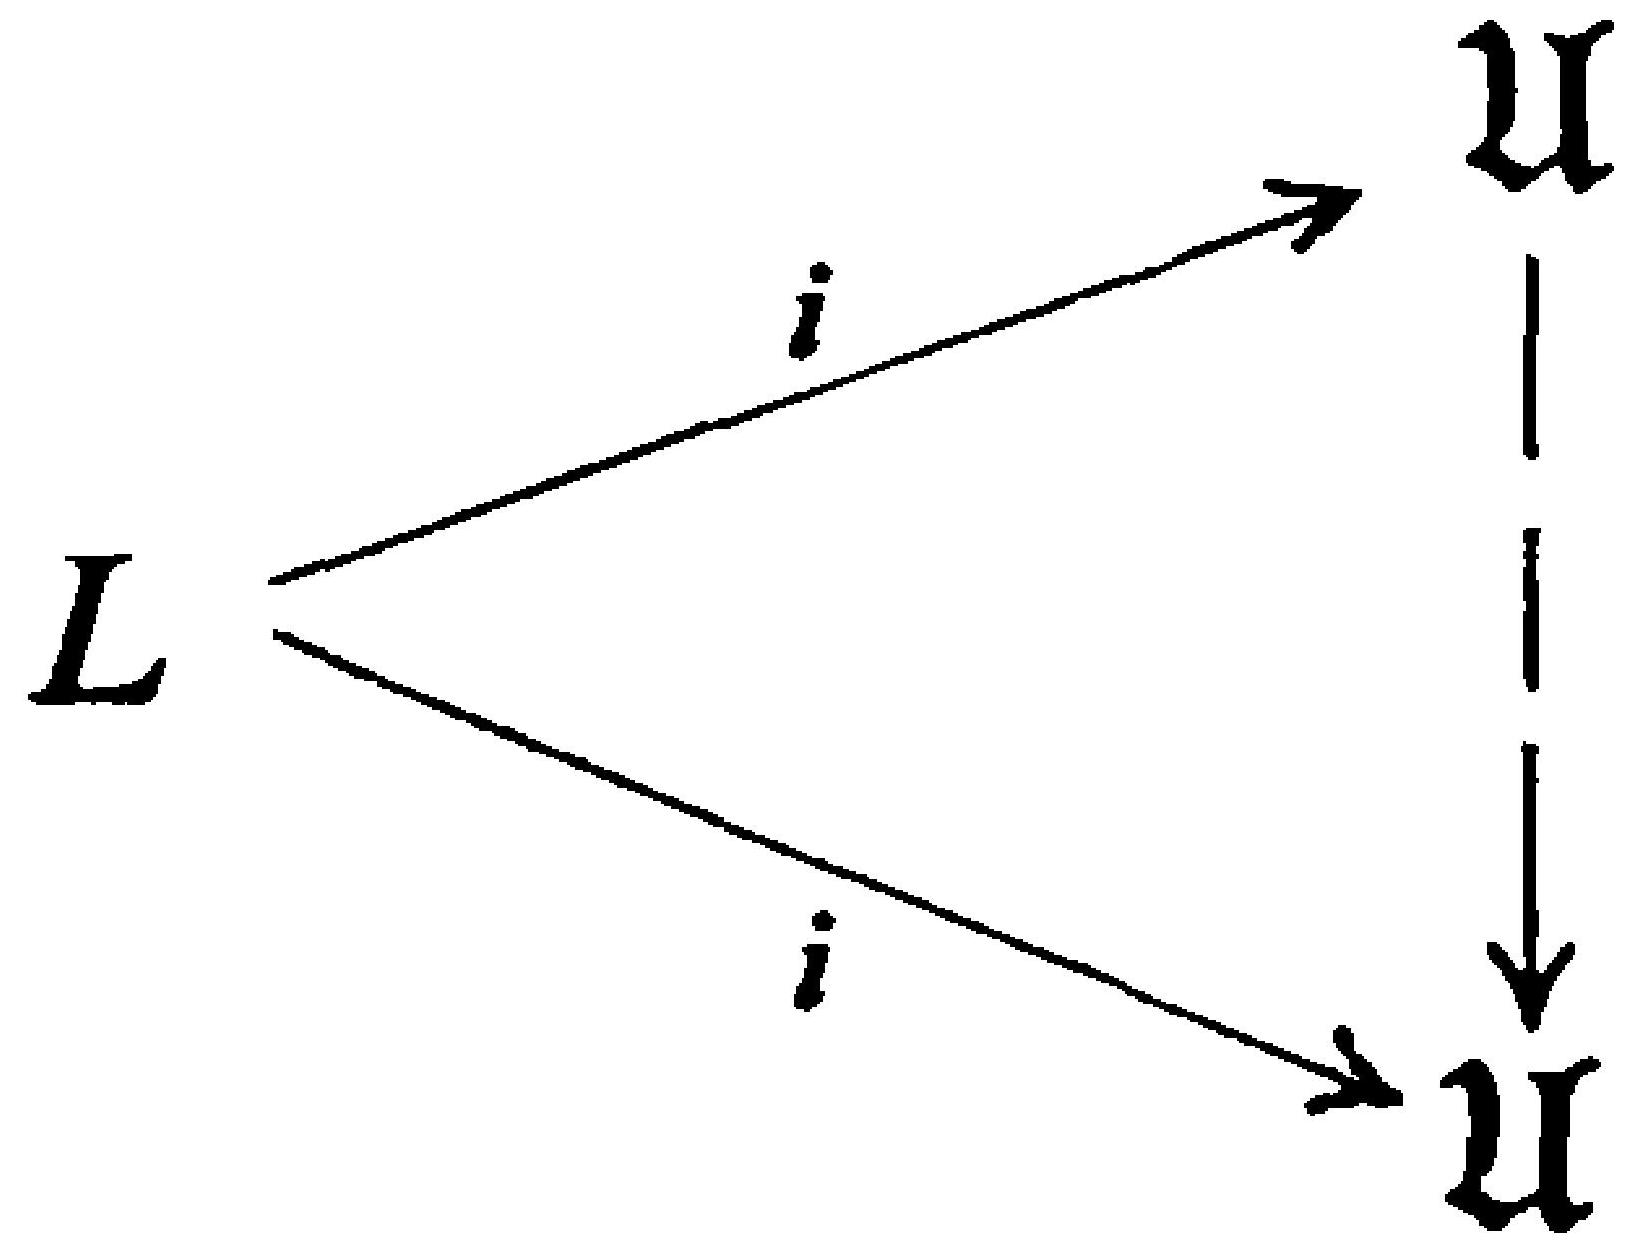
\includegraphics[max width=\textwidth, center]{2025_06_06_fac2836a92464059da43g-103}

But $1_{\mathfrak{U}}$ and $\psi \circ \phi$ both do the trick, so $\psi \circ \phi=1_{\mathfrak{U}}$. Similarly, $\phi \circ \psi=1_{\mathfrak{B}}$. Existence of a suitable pair ( $\mathfrak{U}, i$ ) is also not difficult to establish. Let $\mathcal{T}(L)$ be the tensor algebra on $L(17.1)$, and let $J$ be the two sided ideal in $\mathfrak{I}(L)$ generated by all $x \otimes y-y \otimes x-[x y](x, y \in L)$. Define $\mathfrak{U}(L)=\mathfrak{I}(L) / J$, and let $\pi: \mathfrak{I}(L) \rightarrow \mathfrak{U}(L)$ be the canonical homomorphism. Notice that $J \subset \coprod_{i>0} T^{i} L$, so $\pi$ maps $T^{0} L=\mathrm{F}$ isomorphically into $\mathfrak{U}(L)$ (therefore, $\mathfrak{U}(L)$ contains at least the scalars). It is not at all obvious that $\pi$ maps $T^{1} L=L$ isomorphically into $\mathfrak{U}(L)$; this will be proved later. In any case, we claim that $(\mathfrak{U}(L), i)$ is a universal enveloping algebra of $L$, where $i: L \rightarrow \mathfrak{U}(L)$ is the restriction of $\pi$ to $L$. Indeed, let $j: L \rightarrow \mathfrak{A}$ be as in the definition. The universal property of $\mathfrak{I}(L)$ yields an algebra homomorphism $\phi^{\prime}: \mathfrak{T}(L) \rightarrow \mathfrak{A}$ which extends $j$ and sends 1 to 1 . The special property (*) of $j$ forces all $x \otimes y-y \otimes x-[x y]$ to lie in $\operatorname{Ker} \phi^{\prime}$, so $\phi^{\prime}$ induces a homomorphism $\phi$ : $\mathfrak{U}(L) \rightarrow \mathfrak{A}$ such that $\phi \circ i=j$. The uniqueness of $\phi$ is evident, since 1 and Im $i$ together generate $\mathfrak{U}(L)$.

Example. Let $L$ be abelian. Then the ideal $J$ above is generated by all $x \otimes y-y \otimes x$, hence coincides with the ideal $I$ introduced in (17.1). This means that $\mathfrak{U}(L)$ coincides with the symmetric algebra $\mathfrak{S}(L)$. (In particular, $i: L \rightarrow \mathfrak{U}(L)$ is injective here.)

\subsection*{17.3. PBW Theorem and consequences}
So far we know very little about the structure of $\mathfrak{U}(L)$, except that it contains the scalars. For brevity, write $\mathfrak{I}=\mathfrak{I}(L), \mathfrak{G}=\mathfrak{G}(L), \mathfrak{U}=\mathfrak{U}(L)$; similarly, write $T^{m}, S^{m}$. Define a filtration on $\mathfrak{I}$ by $T_{m}=T^{0} \oplus T^{1} \oplus \ldots \oplus$ $T^{m}$, and let $U_{m}=\pi\left(T_{m}\right), U_{-1}=0$. Clearly, $U_{m} U_{p} \subset U_{m+p}$ and $U_{m} \subset U_{m+1}$. Set $G^{m}=U_{m} / U_{m-1}$ (this is just a vector space), and let the multiplication in $\mathfrak{U}$ define a bilinear map $G^{m} \times G^{p} \rightarrow G^{m+p}$. (The map is well-defined; why?) This extends at once to a bilinear map $\mathfrak{F} \times \mathfrak{F} \rightarrow \mathfrak{F}, \mathfrak{F}=\coprod_{m=0}^{\infty} G^{m}$, making $\mathfrak{F}$ a graded associative algebra with 1.

Since $\pi$ maps $T^{m}$ into $U_{m}$, the composite linear map $\phi_{m}: T^{m} \rightarrow U_{m} \rightarrow G^{m}$ $=U_{m} / U_{m-1}$ makes sense. It is surjective, because $\pi\left(T_{m}-T_{m-1}\right)=U_{m}-U_{m-1}$. The maps $\phi_{m}$ therefore combine to yield a linear map $\phi: \mathfrak{I} \rightarrow \mathfrak{F}$, which is surjective (and sends 1 to 1 ).

Lemma. $\phi: \mathfrak{I} \rightarrow \mathfrak{F}$ is an algebra homomorphism. Moreover, $\phi(I)=0$, so $\phi$ induces a homomorphism $\omega$ of $\mathfrak{G}=\mathfrak{I} /$ I onto $\mathfrak{W}$.

Proof. Let $x \in T^{m}, y \in T^{p}$ be homogeneous tensors. By definition of the product in $\mathfrak{F}, \phi(x y)=\phi(x) \phi(y)$, so it follows that $\phi$ is multiplicative on $\mathfrak{I}$. Let $x \otimes y-y \otimes x(x, y \in L)$ be a typical generator of $I$. Then $\pi(x \otimes y-$ $y \otimes x) \in U_{2}$, by definition. On the other hand, $\pi(x \otimes y-y \otimes x)=\pi([x y]) \in$ $U_{1}$, whence $\phi(x \otimes y-y \otimes x) \in U_{1} / U_{1}=0$. It follows that $I \subset \operatorname{Ker} \phi . \quad \square$

The following theorem is the basic result about $\mathfrak{U}(L)$; it (or its Corollary\\
C) is called the Poincaré-Birkhoff-Witt Theorem (or PBW Theorem). The proof will be given in (17.4).

Theorem. The homomorphism $\omega: \mathfrak{S} \rightarrow \mathfrak{W}$ is an isomorphism of algebras.\\
Corollary A. Let $W$ be a subspace of $T^{m}$. Suppose the canonical map $T^{m} \rightarrow$ $S^{m}$ sends $W$ isomorphically onto $S^{m}$. Then $\pi(W)$ is a complement to $U_{m-1}$ in $U_{m}$.

Proof. Consider the diagram (all maps canonical):\\
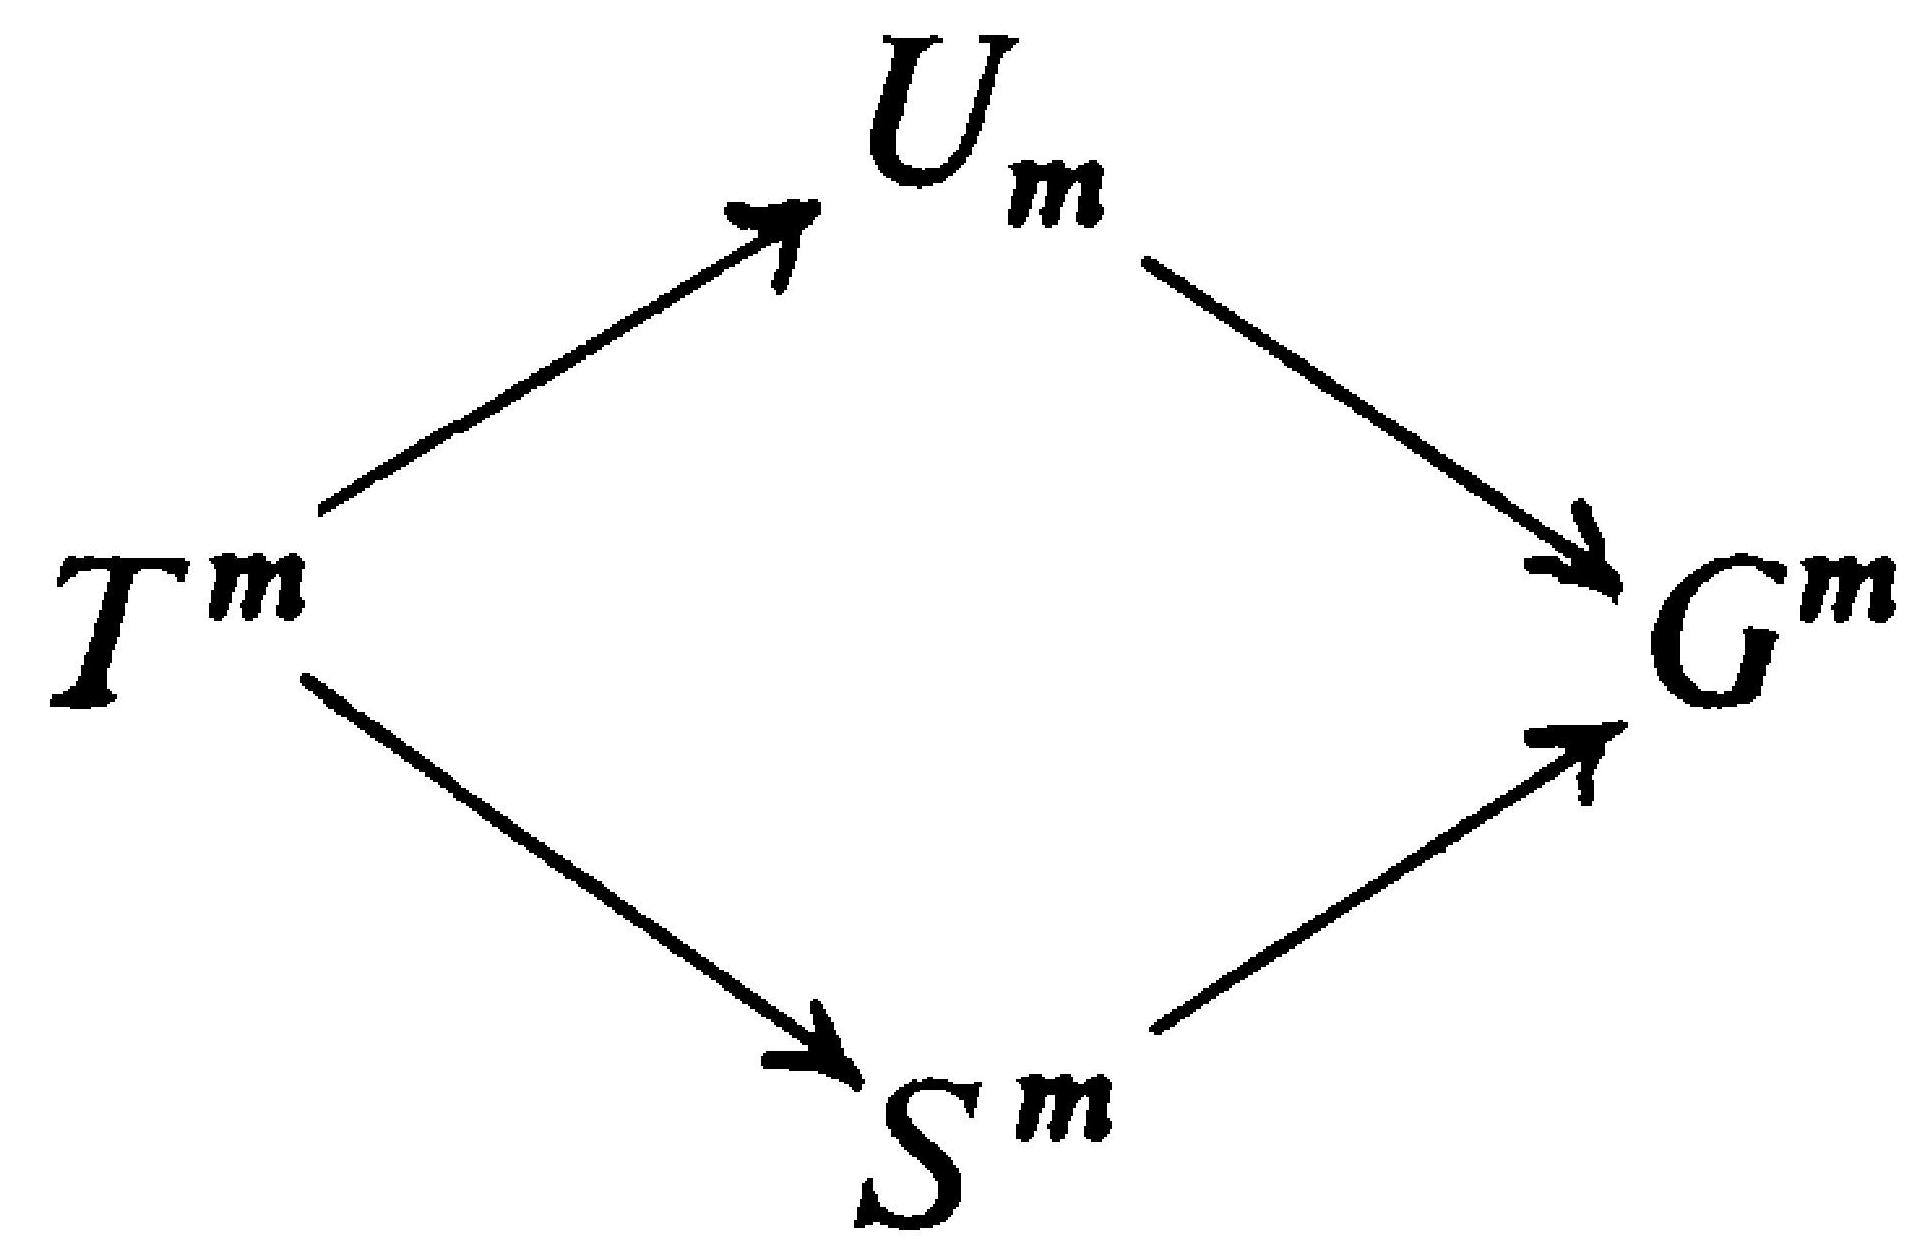
\includegraphics[max width=\textwidth, center]{2025_06_06_fac2836a92464059da43g-105}

Thanks to the lemma above (and the definitions), this is a commutative diagram. Since $\omega: \mathfrak{S} \rightarrow \mathfrak{W}$ is an isomorphism (by the theorem), the bottom map sends $W \subset T^{m}$ isomorphically onto $G^{m}$. Reverting to the top map, we get the corollary.

Corollary B. The canonical map $i: L \rightarrow \mathfrak{U}(L)$ is injective (so $L$ may be identified with $i(L))$.

Proof. This is the special case $W=T^{1}(=L)$ of Corollary A.\\
We have allowed $L$ to be infinite dimensional. In practice, the case where $L$ has countable basis is quite adequate for our purposes.

Corollary C. Let ( $x_{1}, x_{2}, x_{3}, \ldots$ ) be any ordered basis of $L$. Then the elements $x_{i(1)} \ldots x_{i(m)}=\pi\left(x_{i(1)} \otimes \ldots \otimes x_{i(m)}\right), m \in \mathbf{Z}^{+}, i(1) \leq i(2) \ldots \leq$ $i(m)$, along with 1 , form a basis of $\mathfrak{U}(L)$.

Proof. Let $W$ be the subspace of $T^{m}$ spanned by all $x_{i(1)} \otimes \ldots \otimes x_{i(m)}$, $i(1) \leq \ldots \leq i(m)$. Evidently $W$ maps isomorphically onto $S^{m}$, so Corollary A shows that $\pi(W)$ is a complement to $U_{m-1}$ in $U_{m}$.

A basis of $\mathfrak{U}(L)$ of the type just constructed will be referred to simply as a PBW basis.

Corollary D. Let $H$ be a subalgebra of $L$, and extend an ordered basis $\left(h_{1}, h_{2}, \ldots\right)$ of $H$ to an ordered basis $\left(h_{1}, \ldots, x_{1}, \ldots\right)$ of $L$. Then the homomorphism $\mathfrak{U}(H) \rightarrow \mathfrak{U}(L)$ induced by the injection $H \rightarrow L \rightarrow \mathfrak{U}(L)$ is itself injective, and $\mathfrak{U}(L)$ is a free $\mathfrak{U}(H)$-module with free basis consisting of all $x_{i(1)} \ldots x_{i(m)}, i(1) \leq i(2) \leq \ldots \leq i(m)$, along with 1 .

Proof. These assertions follow at once from Corollary C.\\
For use much later, we record a special fact.\\
Corollary E. Let char $\mathrm{F}=0$. With notation as in (17.1), the composite $S^{m} L \rightarrow \widetilde{S}^{m} L \rightarrow U_{m}$ of canonical maps is a (linear) isomorphism of $S^{m} L$ onto a complement of $U_{m-1}$ in $U_{m}$.

Proof. Use Corollary A, with $W=\widetilde{S}^{m}$.

\subsection*{17.4. Proof of PBW Theorem}
Fix an ordered basis ( $x_{\lambda} ; \lambda \in \Omega$ ) of $L$. This choice identifies $\mathfrak{S}$ with the polynomial algebra in indeterminates $z_{\lambda}(\lambda \in \Omega)$. For each sequence $\Sigma=$ $\left(\lambda_{1}, \ldots, \lambda_{m}\right)$ of indices ( $m$ is called the length of $\Sigma$ ), let $z_{\Sigma}=z_{\lambda_{1}} \ldots z_{\lambda_{m}} \in S^{m}$ and let $x_{\Sigma}=x_{\lambda_{1}} \otimes \ldots \otimes x_{\lambda_{m}} \in T^{m}$. Call $\Sigma$ increasing if $\lambda_{1} \leq \lambda_{2} \leq \ldots \leq \lambda_{m}$, in the given ordering of $\Omega$; by fiat, $\varnothing$ is increasing and $z_{\varnothing}=1$. So $\left\{z_{\Sigma} \mid \Sigma\right.$ increasing $\}$ is a basis of $\mathfrak{S}$. Associated with the grading $\mathfrak{S}=\amalg S^{m}$ is the filtration $S_{m}=S^{0} \oplus \ldots \oplus S^{m}$. In the following lemmas, write $\lambda \leq \Sigma$ if $\lambda \leq \mu$ for all $\mu \in \Sigma$.

Lemma A. For each $m \in \mathbf{Z}^{+}$, there exists a unique linear map $f_{m}: L \otimes S_{m}$ $\rightarrow \mathbb{G}$ satisfying:

$$
\begin{aligned}
& \left(A_{m}\right) f_{m}\left(x_{\lambda} \otimes z_{\Sigma}\right)=z_{\lambda} z_{\Sigma} \text { for } \lambda \leq \Sigma, z_{\Sigma} \in S_{m} \\
& \left(B_{m}\right) f_{m}\left(x_{\lambda} \otimes z_{\Sigma}\right)-z_{\lambda} z_{\Sigma} \in S_{k} \text { for } k \leq m, z_{\Sigma} \in S_{k} \\
& \left(C_{m}\right) f_{m}\left(x_{\lambda} \otimes f_{m}\left(x_{\mu} \otimes z_{T}\right)\right)=f_{m}\left(x_{\mu} \otimes f_{m}\left(x_{\lambda} \otimes z_{T}\right)\right)+f_{m}\left(\left[x_{\lambda} x_{\mu}\right] \otimes z_{T}\right) \text { for all } \\
& \quad z_{T} \in S_{m-1}
\end{aligned}
$$

Moreover, the restriction of $f_{m}$ to $L \otimes S_{m-1}$ agrees with $f_{m-1}$.\\
Proof. Notice that the terms in ( $C_{m}$ ) all make sense, once ( $B_{m}$ ) is proved. Notice too that the restriction of $f_{m}$ to $L \otimes S_{m-1}$ automatically satisfies $\left(A_{m-1}\right),\left(B_{m-1}\right),\left(C_{m-1}\right)$, so this restricted map must coincide with $f_{m-1}$ because of the asserted uniqueness. To verify existence and uniqueness of $f_{m}$, we proceed by induction on $m$. For $m=0$, only $z_{\Sigma}=1$ occurs; therefore we may let $f_{0}\left(x_{\lambda} \otimes 1\right)=z_{\lambda}$ (and extend linearly to $L \otimes S_{0}$ ). Evidently $\left(A_{0}\right)$, $\left(B_{0}\right),\left(C_{0}\right)$ are satisfied, and moreover, $\left(A_{0}\right)$ shows that our choice of $f_{0}$ is the only possible one.

Assuming the existence of a unique $f_{m-1}$ satisfying $\left(A_{m-1}\right),\left(B_{m-1}\right)$, $\left(C_{m-1}\right)$, we shall show how to extend $f_{m-1}$ to a map $f_{m}$. For this it will suffice to define $f_{m}\left(x_{\lambda} \otimes z_{\Sigma}\right)$ when $\Sigma$ is an increasing sequence of length $m$.

For the case $\lambda \leq \Sigma,\left(A_{m}\right)$ cannot hold unless we define $f_{m}\left(x_{\lambda} \otimes z_{\Sigma}\right)=$ $z_{\lambda} z_{\Sigma}$. In case $\lambda \leq \Sigma$ fails, the first index $\mu$ in $\Sigma$ must be strictly less than $\lambda$, so $\Sigma=(\mu, T)$, where of course $\mu \leq T$ and $T$ has length $m-1$. By $\left(A_{m-1}\right)$, $z_{\Sigma}=z_{\mu} z_{T}=f_{m-1}\left(x_{\mu} \otimes z_{T}\right)$. Since $\mu \leq T, f_{m}\left(x_{\mu} \otimes z_{T}\right)=z_{\mu} z_{T}$ is already defined, so the left side of $\left(C_{m}\right)$ becomes $f_{m}\left(x_{\lambda} \otimes z_{\Sigma}\right)$. On the other hand, $\left(B_{m-1}\right)$ implies that $f_{m}\left(x_{\lambda} \otimes z_{T}\right)=f_{m-1}\left(x_{\lambda} \otimes z_{T}\right) \equiv z_{\lambda} z_{T}\left(\bmod S_{m-1}\right)$. This shows that the right side of $\left(C_{m}\right)$ is already defined:

$$
z_{\mu} z_{\lambda} z_{T}+f_{m-1}\left(x_{\mu} \otimes y\right)+f_{m-1}\left(\left[x_{\lambda} x_{\mu}\right] \otimes z_{T}\right), y \in S_{m-1} .
$$

The preceding remarks show that $f_{m}$ can be defined, and in only one way. Moreover, $\left(A_{m}\right)$ and $\left(B_{m}\right)$ clearly hold, as does $\left(C_{m}\right)$ in case $\mu<\lambda, \mu \leq T$. But $\left[x_{\mu} x_{\lambda}\right]=-\left[x_{\lambda} x_{\mu}\right]$, so $\left(C_{m}\right)$ also holds for $\lambda<\mu, \lambda \leq T$. When $\lambda=\mu$, ( $C_{m}$ ) is also true. It remains only to consider the case where neither $\lambda \leq T$ nor $\mu \leq T$ is true. Write $T=(\nu, \Psi)$, where $\nu \leq \Psi, \nu<\lambda, \nu<\mu$. To keep the notation under control, abbreviate $f_{m}(x \otimes z)$ by $x z$ whenever $x \in L, z \in S_{m}$.

The induction hypothesis insures that $x_{\mu} z_{T}=x_{\mu}\left(x_{\nu} z_{\Psi}\right)=x_{\nu}\left(x_{\mu} z_{\Psi}\right)+\left[x_{\mu}\right.$ $\left.x_{v}\right] z_{\Psi}$, and $x_{\mu} z_{\Psi}=z_{\mu} z_{\Psi}+w\left(w \in S_{m-2}\right)$, by ( $B_{m-2}$ ). Since $\nu \leq \Psi, \nu<\mu,\left(C_{m}\right)$ applies already to $x_{\lambda}\left(x_{\nu}\left(z_{\mu} z_{\Psi}\right)\right)$. By induction, $\left(C_{m}\right)$ also applies to $x_{\lambda}\left(x_{\nu} w\right)$, therefore to $x_{\lambda}\left(x_{\nu}\left(x_{\mu} z_{\Psi}\right)\right)$. Consequently: $\left({ }^{*}\right) x_{\lambda}\left(x_{\mu} z_{T}\right)=x_{\nu}\left(x_{\lambda}\left(x_{\mu} z_{\Psi}\right)\right)+\left[x_{\lambda}\right.$ $\left.\left.x_{v}\right]\left(x_{\mu} z_{\Psi}\right)+\left[\begin{array}{ll}x_{\mu} & x_{v}\end{array}\right]\left(x_{\lambda} z_{\Psi}\right)+\left[\begin{array}{ll}x_{\lambda} & {\left[x_{\mu}\right.} \\ x_{v}\end{array}\right]\right] z_{\Psi}$.

Recall that $\lambda, \mu$ are interchangeable throughout this argument. If we interchange them in (*) and subtract the two resulting equations, we get:

$$
\begin{aligned}
x_{\lambda}\left(x_{\mu} z_{T}\right) & -x_{\mu}\left(x_{\lambda} z_{T}\right)=x_{v}\left(x_{\lambda}\left(x_{\mu} z_{\Psi}\right)\right)-x_{\nu}\left(x_{\mu}\left(x_{\lambda} z_{\Psi}\right)\right)+\left[x_{\lambda}\left[x_{\mu} x_{v}\right]\right] z_{\Psi}- \\
& -\left[x_{\mu}\left[x_{\lambda} x_{v}\right]\right] z_{\Psi}=x_{v}\left(\left[x_{\lambda} x_{\mu}\right] z_{\Psi}\right)+\left[x_{\lambda}\left[x_{\mu} x_{v}\right]\right] z_{\Psi} \\
& +\left[x_{\mu}\left[x_{v} x_{\lambda}\right]\right] z_{\Psi}=\left[x_{\lambda} x_{\mu}\right]\left(x_{v} z_{\Psi}\right)+\left(\left[x_{v}\left[x_{\lambda} x_{\mu}\right]\right]\right. \\
& \left.+\left[x_{\lambda}\left[x_{\mu} x_{v}\right]\right]+\left[x_{\mu}\left[x_{v} x_{\lambda}\right]\right]\right) z_{\Psi}=\left[x_{\lambda} x_{\mu}\right] z_{T}
\end{aligned}
$$

(thanks to the Jacobi identity).\\
This proves ( $C_{m}$ ), and with it the lemma.\\
Lemma B. There exists a representation $\rho: L \rightarrow \mathfrak{g l}(\mathfrak{S})$ satisfying:\\
(a) $\rho\left(x_{\lambda}\right) z_{\Sigma}=z_{\lambda} z_{\Sigma}$ for $\lambda \leq \Sigma$.\\
(b) $\rho\left(x_{\lambda}\right) z_{\Sigma} \equiv z_{\lambda} z_{\Sigma}\left(\bmod S_{m}\right)$, if $\Sigma$ has length $m$.

Proof. Lemma A allows us to define a linear map $f: L \otimes \mathbb{G} \rightarrow \mathbb{G}$ satisfying $\left(A_{m}\right),\left(B_{m}\right),\left(C_{m}\right)$ for all $m$ (since $f_{m}$ restricted to $L \otimes S_{m-1}$ is $f_{m-1}$, by the uniqueness part). In other words $\mathbb{S}$ becomes an $L$-module (condition $\left(C_{m}\right)$ ), affording a representation $\rho$ which satisfies (a), (b), thanks to $\left(A_{m}\right)$, ( $B_{m}$ ).

Lemma C. Let $t \in T_{m} \cap J(J=\operatorname{Ker} \pi, \pi: \mathfrak{T} \rightarrow \mathfrak{U}$ canonical). Then the homogeneous component $t_{m}$ of $t$ of degree $m$ lies in $I$ (the kernel of the canonical map $\mathfrak{I} \rightarrow \mathfrak{S}$ ).

Proof. Write $t_{m}$ as linear combination of basis elements $x_{\Sigma(i)}(1 \leq i \leq r)$, each $\Sigma(i)$ of length $m$. The Lie homomorphism $\rho: L \rightarrow \mathrm{gl}(\mathbb{G})$ constructed in Lemma B extends, by the universal property of $\mathfrak{U}$, to an algebra homomorphism (also called $\rho$ ) $\mathfrak{I} \rightarrow$ End $\mathfrak{G}$, with $J \subset \operatorname{Ker} \rho$. So $\rho(t)=0$. But $\rho(t) .1$ is a polynomial whose term of highest degree is the appropriate combination of the $z_{\Sigma(i)}(1 \leq i \leq r)$, by Lemma B. Therefore this combination of the $z_{\Sigma(i)}$ is 0 in $\mathfrak{S}$, and $t_{m} \in I$ as required.

Proof of PBW Theorem. Let $t \in T^{m}, \pi: \mathfrak{T} \rightarrow \mathfrak{U}$ the canonical map. We must show that $\pi(t) \in U_{m-1}$ implies $t \in I$. But $t \in T^{m}, \pi(t) \in U_{m-1}$ together imply that $\pi(t)=\pi\left(t^{\prime}\right)$ for some $t^{\prime} \in T_{m-1}$, whence $t-t^{\prime} \in J$. Apply Lemma C to the tensor $t-t^{\prime} \in T_{m} \cap J$ : the homogeneous component of degree $m$ being $t$, we get $t \in I$.

\subsection*{17.5. Free Lie algebras}
The reader may be familiar with the method of constructing groups by generators and relations. We shall use an analogous method in §18 to construct semisimple Lie algebras. For this one needs the notion of free Lie algebra.

Let $L$ be a Lie algebra over F generated by a set $X$. We say $L$ is free\\
on $\mathbf{X}$ if, given any mapping $\phi$ of $X$ into a Lie algebra $M$, there exists a unique homomorphism $\psi: L \rightarrow M$ extending $\phi$. The reader can easily verify the uniqueness (up to a unique isomorphism) of such an algebra $L$. As to its existence, we begin with a vector space $V$ having $X$ as basis, form the tensor algebra $\mathfrak{I}(V)$ (viewed as Lie algebra via the bracket operation), and let $L$ be the Lie subalgebra of $\mathfrak{I}(V)$ generated by $X$. Given any map $\phi$ : $X \rightarrow M$, let $\phi$ be extended first to a linear map $V \rightarrow M \subset \mathfrak{U}(M)$, then (canonically) to an associative algebra homomorphism $\mathfrak{I}(V) \rightarrow \mathfrak{U}(M)$, or a Lie homomorphism (whose restriction to $L$ is the desired $\psi: L \rightarrow M$, since $\psi$ maps the generators $X$ into $M$ ).

We remark that if $L$ is free on a set $X$, then a vector space $V$ can be given an $L$-module structure simply by assigning to each $x \in X$ an element of the Lie algebra $\mathfrak{g l}(V)$ and extending canonically.

Finally, if $L$ is free on $X$, and if $R$ is the ideal of $L$ generated by elements $f_{j}$ ( $j$ running over some index set), we call $L / R$ the Lie algebra with generators $x_{i}$ and relations $f_{j}=0$, where $x_{i}$ are the images in $L / R$ of the elements of $X$.

\section*{Exercises}
\begin{enumerate}
  \item Prove that if $\operatorname{dim} L<\infty$, then $\mathfrak{U}(L)$ has no zero divisors. [Hint: Use the fact that the associated graded algebra $\mathfrak{F}$ is isomorphic to a polynomial algebra.]
  \item Let $L$ be the two dimensional nonabelian Lie algebra (1.4), with $[x y]=x$. Prove directly that $i: L \rightarrow \mathfrak{U}(L)$ is injective (i.e., that $J \cap L=0$ ).
  \item If $x \in L$, extend ad $x$ to an endomorphism of $\mathfrak{U}(L)$ by defining ad $x(y)=$ $x y-y x(y \in \mathfrak{U}(L))$. If $\operatorname{dim} L<\infty$, prove that each element of $\mathfrak{U}(L)$ lies in a finite dimensional $L$-submodule. [If $x, x_{1}, \ldots, x_{m} \in L$, verify that ad $x\left(x_{1} \ldots x_{m}\right)=\sum_{i=1}^{m} x_{1} x_{2} \ldots$ ad $x\left(x_{i}\right) \cdot x_{m}$.]
  \item If $L$ is a free Lie algebra on a set $X$, prove that $\mathfrak{U}(L)$ is isomorphic to the tensor algebra on a vector space having $X$ as basis.
  \item Describe the free Lie algebra on a set $X=\{x\}$.
  \item How is the PBW Theorem used in the construction of free Lie algebras?
\end{enumerate}

\section*{Notes}
Our treatment of the PBW Theorem follows Bourbaki [1]. For another approach, see Jacobson [1].

\section*{18. Generators and relations}
We can now resume our study of a semisimple Lie algebra $L$ over the algebraically closed field $F$ of characteristic 0 . The object is to find a pre-\\
sentation of $L$ by generators and relations which depend only on the root system $\Phi$, thereby proving both the existence and the uniqueness of a semisimple Lie algebra having $\Phi$ as root system. In this section, contrary to our general convention, Lie algebras are allowed to be infinite dimensional.

\subsection*{18.1. Relations satisfied by L}
Let $L$ be a semisimple Lie algebra, $H$ a CSA, $\Phi$ the corresponding root system, $\Delta=\left\{\alpha_{1}, \ldots, \alpha_{\ell}\right\}$ a fixed base. Recall that $\left\langle\alpha_{i}, \alpha_{j}\right\rangle=\frac{2\left(\alpha_{i}, \alpha_{j}\right)}{\left(\alpha_{j}, \alpha_{j}\right)}=$ $\alpha_{i}\left(h_{j}\right)\left(h_{j}=h_{\alpha_{j}}\right)$. Fix a standard set of generators $x_{i} \in L_{\alpha_{i}}, y_{i} \in L_{-\alpha_{i}}$, so that $\left[x_{i} y_{i}\right]=h_{i}$.

Proposition. With the above notation, $L$ is generated by $\left\{x_{i}, y_{i}, h_{i} \mid 1 \leq i \leq\right.$ $\ell\}$, and these generators satisfy at least the following relations:\\
$(S 1)\left[h_{i} h_{j}\right]=0$ $(1 \leq i, j \leq \ell)$.\\
(S2) $\left[x_{i} y_{i}\right]=h_{i},\left[x_{i} y_{j}\right]=0$ if $i \neq j$.\\
$(S 3)\left[h_{i} x_{j}\right]=\left\langle\alpha_{j}, \alpha_{i}\right\rangle x_{j},\left[h_{i} y_{j}\right]=-\left\langle\alpha_{j}, \alpha_{i}\right\rangle y_{j}$.\\
$\left(S_{i j}^{+}\right)\left(a d x_{i}\right)^{-\left\langle\alpha_{j}, \alpha_{i}\right\rangle+1}\left(x_{j}\right)=0$\\
$(i \neq j)$.\\
$\left(S_{i j}^{-}\right)\left(a d y_{i}\right)^{-\left\langle\alpha_{j}, \alpha_{i}\right\rangle+1}\left(y_{j}\right)=0$\\
$(i \neq j)$.\\
Proof. Proposition 14.2 implies that $L$ is already generated by the $x_{i}$ and $y_{i}$. Relation (S1) is clear, as is (S2), in view of the fact that $\alpha_{i}-\alpha_{j} \notin \Phi$ when $i \neq j$ (Lemma 10.1). (S3) is obvious. Consider now ( $S_{i j}^{+}$) (( $S_{i j}^{-}$) will follow by symmetry). Since $i \neq j, \alpha_{j}-\alpha_{i}$ is not a root, and the $\alpha_{i}$-string through $\alpha_{j}$ consists of $\alpha_{j}, \alpha_{j}+\alpha_{i}, \ldots, \alpha_{j}+q \alpha_{i}$, where $-q=\left\langle\alpha_{j}, \alpha_{i}\right\rangle$ (see (9.4) or Proposition 8.4(e)). Since ad $x_{i}$ maps $x_{j}$ successively into the root spaces for $\alpha_{j}+\alpha_{i}, \alpha_{j}+2 \alpha_{i}, \ldots,\left(S_{i j}^{+}\right)$follows.

Notice that the relations in the proposition involve constants which depend only on the root system. Serre discovered that these form a complete set of defining relations for $L$ (Theorem 18.3 below). As a first step toward proving Serre's Theorem, we shall examine the (possibly infinite dimensional) Lie algebra defined by (S1)-(S3) alone.

\subsection*{18.2. Consequences of (S1)-(S3)}
Fix a root system $\Phi$, with base $\Delta=\left\{\alpha_{1}, \ldots, \alpha_{\ell}\right\}$. Abbreviate the Cartan integer $\left\langle\alpha_{i}, \alpha_{j}\right\rangle$ by $c_{i j}$. We begin with a free Lie algebra $\hat{L}$ (see (17.4)) on $3 \ell$ generators $\left\{\hat{x}_{i}, \hat{y}_{i}, \hat{h}_{i} \mid 1 \leq i \leq \ell\right\}$. Let $\hat{K}$ be the ideal in $\hat{L}$ generated by the following elements: $\left[\hat{h}_{i} \hat{h}_{j}\right],\left[\hat{x}_{i} \hat{y}_{j}\right]-\delta_{i j} \hat{h}_{i},\left[\hat{h}_{i} \hat{x}_{j}\right]-c_{j i} \hat{x}_{j},\left[\hat{h}_{i} \hat{y}_{j}\right]+c_{j i} \hat{y}_{j}$. Set $L_{o}=$ $\hat{L} / \widehat{K}$, and let $x_{i}, y_{i}, h_{i}$ be the respective images in $L_{o}$ of the generators. (In general, $\operatorname{dim} L_{o}=\infty$.)

The trouble with $L_{o}$ is that it is defined too abstractly (it might even be trivial, for all we know at this point). To study $L_{o}$ concretely we attempt to construct a suitable representation of it. The construction which follows is\\
the prototype of one which plays a prominent role in Chapter VI, so the reader is urged to follow the argument closely.

As was noted in (17.5), there is no problem about constructing a module for $\hat{L}$ : we need only specify a linear transformation corresponding to each of the $3 \ell$ generators. Let $V$ be the tensor algebra ( $=$ free associative algebra) on a vector space with basis $\left(v_{1}, \ldots, v_{\ell}\right)$, but forget the product in $V$. To avoid cumbersome notation we abbreviate $v_{i_{1}} \otimes \ldots \otimes v_{i_{t}}$ by $v_{i_{1}} \ldots v_{i_{t}}$. These tensors (along with 1) form a basis of $V$ over F . Next, define endomorphisms of $V$ as follows:

$$
\begin{aligned}
& \left\{\begin{array}{l}
\hat{h}_{j \cdot 1}=0 \\
\hat{h}_{j \cdot} \cdot v_{i_{1}} \ldots v_{i_{t}}=-\left(c_{i_{1} j}+\ldots+c_{i_{t} j}\right) v_{i_{1}} \ldots v_{i_{t}}
\end{array}\right. \\
& \left\{\begin{array}{l}
\hat{y}_{j \cdot} \cdot 1=v_{j} \\
\hat{y}_{j \cdot} \cdot v_{i_{1}} \ldots v_{i_{t}}=v_{j} v_{i_{1}} \ldots v_{i_{t}}
\end{array}\right. \\
& \left\{\begin{array}{l}
\hat{x}_{j \cdot} \cdot 1=0=\hat{x}_{j \cdot} v_{i} \\
\hat{x}_{j \cdot} \cdot v_{i_{1}} \ldots v_{i_{t}}=v_{i_{1}}\left(\hat{x}_{j \cdot} \cdot v_{i_{2}} \ldots v_{i_{t}}\right)-\delta_{i_{1} j}\left(c_{i_{2} j}+\ldots+c_{i_{t} j}\right) v_{i_{2}} \ldots v_{i_{t}}
\end{array}\right.
\end{aligned}
$$

Then there is a (unique) extension to $\hat{L}$ of this action by its generators, yielding a representation $\hat{\phi}: \hat{L} \rightarrow g l(V)$.

Proposition. Let $\hat{K}_{o}=\operatorname{Ker} \hat{\phi}$. Then $\hat{K} \subset \hat{K}_{o}$, i.e., $\hat{\phi}$ factors through $L_{o}$, thereby making $V$ an $L_{o}$-module.

Proof. Notice first that $\hat{h}_{j}$ acts diagonally on $V$ (relative to the chosen basis of V), so that $\hat{\phi}\left(\hat{h}_{i}\right)$ and $\hat{\phi}\left(\hat{h}_{j}\right)$ commute, i.e., $\left[\hat{h}_{i} \hat{h}_{j}\right] \in \hat{K}_{o}$. On the other hand, $\phi\left(\hat{y}_{j}\right)$ is simply left multiplication by $v_{j}$. (It is only the action of $\hat{x}_{j}$ which complicates matters.)

Setting $j=i_{1}$ in the formulas, we obtain: $\hat{x}_{i} \cdot \hat{y}_{j} \cdot v_{i_{2}} \ldots v_{i_{t}}-\hat{y}_{j} \cdot \hat{x}_{i} \cdot v_{i_{2}} \ldots v_{i_{t}}=$ $-\delta_{j i}\left(c_{i_{2} i}+\ldots+c_{i_{t} i}\right) v_{i_{2}} \ldots v_{i_{t}}=\delta_{j i} \hat{h}_{i} \cdot v_{i_{2}} \ldots v_{i_{t}}$. Also, $\left(\hat{x}_{i} \hat{y}_{j}-\hat{y}_{j} \hat{x}_{i}\right) \cdot 1=0=$ $\delta_{i j} \hat{h}_{i}$. . Therefore, $\left[\hat{x}_{i} \hat{y}_{j}\right]-\delta_{i j} \hat{h}_{i} \in \widehat{K}_{o}$.

Next, $\left(\hat{h}_{i} \hat{y}_{j}-\hat{y}_{j} \hat{h}_{i}\right) \cdot 1=\hat{h}_{i} \cdot v_{j}=-c_{j i} v_{j}=-c_{j i} \hat{y}_{j}$. 1. Similarly, $\left(\hat{h}_{i} \hat{y}_{j}-\hat{y}_{j} \hat{h}_{i}\right)$. $v_{i_{1}} \ldots v_{i_{t}}=\hat{h}_{i} \cdot v_{j} v_{i_{1}} \ldots v_{i_{t}}+\left(c_{i_{1} i}+\ldots+c_{i_{t} i}\right) v_{j} v_{i_{1}} \ldots v_{i_{t}}=-c_{j i} \hat{y}_{j} \cdot v_{i_{1}} \ldots v_{i_{t}}$. Therefore, $\left[\hat{h}_{i} \hat{y}_{j}\right]+c_{j i} \hat{y}_{j} \in \hat{K}_{o}$.

For the remaining step, we make a preliminary observation:


\begin{equation*}
\hat{h}_{i} \cdot \hat{x}_{j} \cdot v_{i_{1}} \ldots v_{i_{t}}=-\left(c_{i_{1} i}+\ldots+c_{i_{t} i}-c_{j i}\right) \hat{x}_{j} \cdot v_{i_{1}} \ldots v_{i_{t}} . \tag{*}
\end{equation*}


This is proved by induction on $t$, starting with the case $t=0$ (then $v_{i_{1}} \ldots v_{i_{t}}$ $=1$, by convention), where both sides are 0 . The induction hypothesis just says that $\hat{x}_{j} . v_{i_{2}} \ldots v_{i_{t}}$ is an eigenvector for $\hat{h}_{i}$, with eigenvalue $-\left(c_{i_{2} i}+\ldots+\right.$ $\left.c_{i_{t} i}-c_{j i}\right)$. Multiplying this eigenvector by $v_{i_{1}}$ on the left evidently produces another eigenvector for $\hat{h}_{i}$, with eigenvalue $-\left(c_{i_{1} i}+\ldots+c_{i_{t} i}-c_{j i}\right)$. From these remarks and the definitions (*) follows quickly.

Using (*) we calculate: $\left(\hat{h}_{i} \hat{x}_{j}-\hat{x}_{j} \hat{h}_{i}\right) \cdot 1=0,\left(\hat{h}_{i} \hat{x}_{j}-\hat{x}_{j} \hat{h}_{i}\right) \cdot v_{i_{1}} \ldots v_{i_{t}}=$ $\left(-\left(c_{i_{1} i}+\ldots+c_{i_{t} i}-c_{j i}\right)+\left(c_{i_{1} i}+\ldots+c_{i_{t} i}\right)\right) \hat{x}_{j} \cdot v_{i_{1}} \ldots v_{i_{t}}=c_{j i} \hat{x}_{j} \cdot v_{i_{1}} \ldots v_{i_{t}}$. So $\left[\hat{h}_{i} \hat{x}_{j}\right]-c_{j l} \hat{x}_{j} \in \hat{K}_{o}$. Finally, $\hat{K} \subset \hat{K}_{o}$.

Theorem. Given a root system $\Phi$ with base $\left\{\alpha_{1}, \ldots, \alpha_{\ell}\right\}$, let $L_{o}$ be the Lie\\
algebra with generators $\left\{x_{i}, y_{i}, h_{i} \mid 1 \leq i \leq \ell\right\}$ and relations (S1)-(S3). Then the $h_{i}$ are a basis for an $\ell$-dimensional abelian subalgebra $H$ of $L_{o}$ and $L_{o}=Y$ $+H+X$ (direct sum of subspaces), where $Y$ (resp. $X$ ) is the subalgebra of $L_{o}$ generated by the $y_{i}$ (resp. $x_{i}$ ).

Proof. This proceeds in steps, using the representation $\phi: L_{o} \rightarrow g \mathfrak{l}(V)$ constructed above: $\phi(x)=\hat{\phi}(\hat{x})$ if $x$ is the image in $L_{o}$ of $\hat{x} \in \hat{L}$.\\
(1) $\sum \mathrm{F} \hat{h}_{j} \cap \operatorname{Ker} \hat{\phi}=0$. If $\hat{h}=\sum_{j=1}^{\ell} a_{j} \hat{h}_{j}$, and $\hat{\phi}(\hat{h})=0$, then in particular the eigenvalues $-\sum_{j} a_{j} c_{i j}(1 \leq i \leq \ell)$ of $\hat{\phi}(\hat{h})$ are all 0 . But the Cartan matrix ( $c_{i j}$ ) of $\Phi$ is nonsingular, so this forces all $a_{j}=0$, i.e., $\hat{h}=0$.\\
(2) The canonical map $\hat{L} \rightarrow L_{o}$ sends $\sum \mathrm{F} \hat{h}_{j}$ isomorphically onto $\sum \mathrm{F} h_{j}$. This follows directly from (1).\\
(3) The subspace $\sum \mathrm{F} \hat{x}_{j}+\sum \mathrm{F} \hat{y}_{j}+\sum \mathrm{F} \hat{h}_{j}$ of $\hat{L}$ maps isomorphically into $L_{o}$. Fix $i$. The relations (S1)-(S3) include: $\left[x_{i} y_{i}\right]=h_{i},\left[h_{i} x_{i}\right]=2 x_{i},\left[h_{i} y_{i}\right]=-2 y_{i}$; so $\mathrm{F} x_{i}+\mathrm{F} y_{i}+\mathrm{F} h_{i}$ is a homomorphic image of $\mathfrak{s l}(2, \mathrm{~F})$. But the latter is simple, and $h_{i} \neq 0$ (step (2)), so $\mathrm{F} x_{i}+\mathrm{F} y_{i}+\mathrm{F} h_{i}$ must be isomorphic to $\mathfrak{s l}(2, \mathrm{~F})$. Now the set $\left\{x_{j}, y_{j}, h_{j} \mid 1 \leq j \leq \ell\right\}$ is linearly independent, because its elements are nonzero and satisfy relations (S1)-(S3) (cf. the eigenvalues of the ad $h_{j}$ ). This proves (3).\\
(4) $H=\sum \mathrm{F} h_{j}$ is an $\ell$-dimensional abelian subalgebra of $L_{o}$. This follows from (2) and relation (S1).\\
(5) If $\left[x_{i_{1}} \ldots x_{i_{t}}\right]$ denotes $\left[x_{i_{1}}\left[x_{i_{2}} \ldots\left[x_{i_{t-1}} x_{i_{t}}\right] \ldots\right]\right.$, then $\left[h_{j}\left[x_{i_{1}} \ldots x_{i_{t}}\right]\right]=$ $\left(c_{i_{1} j}+\ldots+c_{i_{t} j}\right)\left[x_{i_{1}} \ldots x_{i_{t}}\right]$, and similarly for the $y_{i}$ in place of the $x_{i},-c_{i j}$ in place of $c_{i j}$. For $t=1$ this is (S3). The general case follows quickly by induction, using the Jacobi identity.\\
(6) If $t \geq 2$, then $\left[y_{j}\left[x_{i_{1}} \ldots x_{i_{t}}\right]\right] \in X$, and similarly for $Y$. By relation (S2), $\left[y_{j} x_{i}\right]=-\delta_{i j} h_{i}$, and therefore the case $t=2$ is immediate from the Jacobi identity and (S3). An easy induction on $t$ completes the argument.\\
(7) $Y+H+X$ is a subalgebra of $L_{o}$, hence coincides with $L_{o}$. That $Y+H+X$ is a subalgebra follows from (4), (5), (6). But $Y+H+X$ contains a set of generators of $L_{o}$, so it coincides with $L_{o}$.\\
(8) The sum $L_{o}=Y+H+X$ is direct. Indeed, (5) shows how to decompose $L_{o}$ into eigenspaces for ad $H$; directness follows (cf. (1), (2)).

It is convenient to describe the decomposition $L_{\boldsymbol{o}}=Y+H+X$ in terms of "weights" (to use the language of §20). For $\lambda \in H^{*}$, let $\left(L_{o}\right)_{\lambda}=\left\{t \in L_{o} \mid[h t]\right.$ $=\lambda(h) t$ for all $h \in H\}$. The proof of the preceding theorem shows that $H=\left(L_{o}\right)_{0}$. Moreover, the only nonzero $\lambda$ for which $\left(L_{o}\right)_{\lambda} \neq 0$ are those of the form $\lambda=\sum_{i=1}^{\ell} k_{i} \alpha_{i}\left(k_{i} \in \mathbf{Z}\right)$, with all $k_{i} \geq 0$ (write $\lambda \succ 0$ in this case) or all $k_{i} \leq 0($ write $\lambda \prec 0)$. Then $X=\sum_{\lambda>0}\left(L_{o}\right)_{\lambda}$ and $Y=\sum_{\lambda<0}\left(L_{o}\right)_{\lambda}$.

\subsection*{18.3. Serre's Theorem}
In (18.2) we studied the structure of the Lie algebra $L_{o}$ determined by (S1)-(S3) alone. Now we ask what happens when we impose the "finiteness"\\
conditions $\left(S_{i j}^{+}\right),\left(S_{i j}^{-}\right)$of $(18.1)$. Set $x_{i j}=\left(\operatorname{ad} x_{i}\right)^{-c_{j i}+1}\left(x_{j}\right), y_{i j}=\left(\operatorname{ad} y_{i}\right)^{-c_{j i}+1}$ $\left(y_{j}\right)(i \neq j)$. (These are elements of $L_{o}$ )

Lemma. In the algebra $L_{o}$ of (18.2), ad $x_{k}\left(y_{i j}\right)=0(1 \leq k \leq \ell)$ for each $i \neq j$.

Proof. Case (a): $k \neq i$. Then $\left[x_{k} y_{i}\right]=0$ (by (S2)), so ad $x_{k}$ and ad $y_{i}$ commute. Therefore, ad $x_{k}\left(y_{i j}\right)=\left(\text { ad } y_{i}\right)^{-c_{j i}+1}$ ad $x_{k}\left(y_{j}\right)$. If $k=j$, this reads (ad $\left.y_{i}\right)^{-c_{j i}+1}\left(h_{j}\right)$. But by (S3), ad $y_{i}\left(h_{j}\right)=c_{i j} y_{i}$. If this is nonzero, then $c_{j i}$ is nonzero (and negative, since $i \neq j$ ), so $-c_{j i}+1 \geq 2$. It follows that $\left(\text { ad } y_{i}\right)^{-c_{j i}+1}\left(h_{j}\right)=0$. If $k \neq j$, then $\left[x_{k} y_{j}\right]=0$ (S2), so the same assertion follows.

Case (b): $k=i$. Recall from the proof of Theorem 18.2 that $S=\mathrm{F}_{x_{i}}+$ $\mathrm{F} y_{i}+\mathrm{F} h_{i}$ is a subalgebra of $L_{o}$ isomorphic to $\mathfrak{s l}(2, \mathrm{~F})$. We can therefore say quite a bit about the adjoint action of $S$ on $L_{o}$. Even though $L_{o}$ is (in general) infinite dimensional, some of the reasoning used in §7 carries over directly to the present situation. In particular, since $j \neq i,\left[x_{i} y_{j}\right]=0$, so that $y_{j}$ is a "maximal vector" for $S$, of "weight" $m=-c_{j i}$ (because $\left[h_{l} y_{J}\right]=-c_{j i} y_{j}$ ). An easy induction on $t$ shows that ad $x_{i}\left(\operatorname{ad} y_{i}\right)^{t}\left(y_{j}\right)=t(m-t+1)\left(\operatorname{ad} y_{i}\right)^{t-1}$ $\left(y_{j}\right)$. Therefore the right side is 0 when $t=-c_{j i}+1$.

Before stating Serre's Theorem, we mention a useful construction. Call an endomorphism $x$ of an infinite dimensional vector space $V$ locally nilpotent if every element of $V$ is killed by a sufficiently large power of $x$. In that case, $x$ is nilpotent on each finite dimensional subspace $W$ of $V$, so it makes sense to form $\exp \left(\left.x\right|_{W}\right)$. It is clear that $\exp \left(\left.x\right|_{W}\right)$ and $\exp \left(\left.x\right|_{W^{\prime}}\right)$ agree on $W \cap W^{\prime}$, so we can patch these maps together to obtain an automorphism "exp $x$ " of $V$.

Theorem (Serre). Fix a root system $\Phi$, with base $\Delta=\left\{\alpha_{1}, \ldots, \alpha_{\ell}\right\}$. Let $L$ be the Lie algebra generated by $3 \ell$ elements $\left\{x_{i}, y_{i}, h_{i} \mid 1 \leq i \leq \ell\right\}$, subject to the relations $(S 1),(S 2),(S 3),\left(S_{i j}^{+}\right),\left(S_{i j}^{-}\right)$listed in (18.1). Then $L$ is a (finite dimensional) semisimple algebra, with CSA spanned by the $h_{i}$ and with corresponding root system $\Phi$.

Proof. This will be carried out in steps. By definition, $L=L_{o} / K, L_{o}$ as in (18.2) and $K$ the ideal generated by all $x_{i j}, y_{i j}(i \neq j)$. To avoid notational problems, we work at first inside $L_{o}$. Let $I$ (resp. $J$ ) be the ideal of $X$ (resp. $Y$ ) generated by all $x_{i j}$ (resp. $y_{i j}$ ). (So $K$ includes $I, J$. )\\
(1) $I$ and $J$ are ideals of $L_{o}$. It suffices to consider $J$ (the argument for $I$ being analogous). On the one hand, $y_{i j}$ is an eigenvector for ad $h_{k}(1 \leq k \leq \ell)$, with eigenvalue $c_{j k}+\left(c_{j i}-1\right) c_{i k}$. Since ad $h_{k}(Y) \subset Y$, it follows from the Jacobi identity that ad $h_{k}(J) \subset J$. On the other hand, the lemma above says that ad $x_{k}\left(y_{i j}\right)=0$. It is clear that ad $x_{k}$ maps $Y$ into $Y+H$ (cf. 18.2)); combining this with the Jacobi identity and the fact that ad $h_{k}(J) \subset J$, we get ad $x_{k}(J) \subset J$. Finally, ad $L_{o}(J) \subset J$, again by the Jacobi identity (since the $x_{k}, y_{k}$ generate $\left.L_{o}\right)$.\\
(2) $K=I+J$. By definition, $I+J \subset K$. But $I+J$ is an ideal of $L_{o}$ (by (1)) containing all $x_{i j}, y_{i j}$, and $K$ is the smallest such ideal.\\
(3) $L=N^{-}+H+N$ (direct sum of subspaces), where $N^{-}=Y / J, N=$ $X / I$, and $H$ is identified with its image under the canonical map $L_{o} \rightarrow L$. Use (2), along with the direct sum decomposition $L_{o}=Y+H+X$ (Theorem 18.2).\\
(4) $\sum \mathrm{F} x_{i}+\sum \mathrm{F} h_{i}+\sum \mathrm{F} y_{i}$ maps isomorphically into $L$. This follows just as in step (3) of the proof of Theorem 18.2, since $H$ maps isomorphically into $L$ (by (3) above). We may therefore identify $x_{i}, y_{i}, h_{i}$ with elements of $L$ (and these generate $L$ ).\\
(5) If $\lambda \in H^{*}$, let $L_{\lambda}=\{x \in L \mid[h x]=\lambda(h) x$ for all $h \in H\}$. Then $H=L_{0}$, $N=\sum_{\lambda>0} L_{\lambda}, N^{-}=\sum_{\lambda<0} L_{\lambda}$ (cf. remarks at end of (18.2)), and each $L_{\lambda}$ is finite dimensional. This is clear, because of (3), (4).\\
(6) For $1 \leq i \leq \ell$, ad $x_{i}$ and ad $y_{i}$ are locally nilpotent endomorphisms of $L$. It suffices to consider ad $x_{i}$, for fixed $i$ (by symmetry). Let $M$ be the subspace of all elements of $L$ which are killed by some power of ad $x_{i}$. If $x \in M(\operatorname{resp} . y \in M)$ is killed by $\left(\operatorname{ad} x_{i}\right)^{r}\left(\operatorname{resp} .\left(\operatorname{ad} x_{i}\right)^{s}\right)$, then $[x y]$ is killed by $\left(\operatorname{ad} x_{i}\right)^{r+s}$ (cf. Lemma 15.1). So $M$ is actually a subalgebra of $L$. But all $x_{k} \in M$ (by relations $\left(S_{i j}^{+}\right)$) and all $y_{k} \in M$ (by (S2), (S3)). These elements generate $L$, so $M=L$, as desired.\\
(7) $\tau_{i}=\exp \left(a d x_{i}\right) \exp \left(a d\left(-y_{i}\right)\right) \exp \left(a d x_{i}\right)($ for $1 \leq i \leq \ell)$ is a welldefined automorphism of $L$. This follows from (6) and the remarks just preceding the theorem.\\
(8) If $\lambda, \mu \in H^{*}$ and $\sigma \lambda=\mu(\sigma \in \mathscr{W}$, the Weyl group of $\Phi)$, then dim $L_{\lambda}=\operatorname{dim} L_{\mu}$. It suffices to prove this when $\sigma=\sigma_{\alpha_{i}}$ is a simple reflection, because these generate $\mathscr{W}$ (Theorem 10.3(d)). The automorphism $\tau_{i}$ of $L$ constructed in step (7) coincides on the finite dimensional space $L_{\lambda}+L_{\mu}$ with the ordinary product of exponentials, and we conclude (as in the last part of (7.2)) that $\tau_{i}$ interchanges $L_{\lambda}, L_{\mu}$. In particular, $\operatorname{dim} L_{\lambda}=\operatorname{dim} L_{\mu}$.\\
(9) For $1 \leq i \leq \ell$, dim $L_{\alpha_{i}}=1$, while $L_{k \alpha_{i}}=0$ for integers $k \neq 0$, 1 , -1. This is clear for $L_{o}$, hence also for $L$ because of (4).\\
(10) If $\alpha \in \Phi$, then $\operatorname{dim} L_{\alpha}=1$, but $L_{k \alpha}=0$ for $k \neq 0,1,-1$. Each root is $\mathscr{W}$-conjugate to a simple root (Theorem 10.3(c)), so this follows from (8), (9).\\
(11) If $L_{\lambda} \neq 0$, then either $\lambda \in \Phi$ or $\lambda=0$. Otherwise $\lambda$ is an integral combination of simple roots, with coefficients of like sign (not all 0 ), $\lambda$ not a multiple of any root because of (10). Exercise 10.10 shows that some $\mathscr{W}$ conjugate $\sigma \lambda$ has a strictly positive as well as a strictly negative coefficient. This means that $L_{\sigma \lambda}=0$ (cf. (5)), contradicting the conclusion of step (8).\\
(12) $\operatorname{dim} L=\ell+\operatorname{Card} \Phi<\infty$. In view of (5), this follows from (10), (11).\\
(13) $L$ is semisimple. Let $A$ be an abelian ideal of $L$; we have to show that $A=0$. Since ad $H$ stabilizes $A, A=(A \cap H)+\sum_{\alpha \in \Phi}\left(A \cap L_{\alpha}\right)$ (because $\left.L=H+\sum_{\alpha \in \Phi} L_{\alpha}\right)$. If $L_{\alpha} \subset A$, then $\left[L_{-\alpha} L_{\alpha}\right] \subset A$, whence $L_{-\alpha} \subset A$ and $A$ contains a copy of the simple algebra $\mathfrak{s l}(2, \mathrm{~F})$ (cf. step (4)). This is absurd, so instead $A=A \cap H \subset H$, whence $\left[L_{\alpha} A\right]=0(\alpha \in \Phi)$ and $A \subset \bigcap_{\alpha \in \Phi} \operatorname{Ker} \alpha$ $=0\left(\right.$ the $\left.\alpha_{i} \operatorname{span} H^{*}\right)$.\\
(14) $H$ is a CSA of $L, \Phi$ the root system. $H$ is abelian (hence nilpotent) and\\
self-normalizing (because of the direct sum decomposition $L=H+\sum_{\alpha \in \Phi} L_{\alpha}$ ), i.e., $H$ is a CSA. Then $\Phi$ is obviously the corresponding set of roots.

\subsection*{18.4. Application: Existence and uniqueness theorems}
Finally, our efforts are rewarded.\\
Theorem. (a) Let $\Phi$ be a root system. Then there exists a semisimple Lie algebra having $\Phi$ as its root system.\\
(b) Let $L, L^{\prime}$ be semisimple Lie algebras, with respective CSA's $H, H^{\prime}$ and root systems $\Phi, \Phi^{\prime}$. Let an isomorphism $\Phi \rightarrow \Phi^{\prime}$ be given, sending a given base $\Delta$ to a base $\Delta^{\prime}$, and denote by $\pi: H \rightarrow H^{\prime}$ the associated isomorphism (as in (14.2)). For each $\alpha \in \Delta\left(\alpha^{\prime} \in \Delta^{\prime}\right)$ select arbitrary nonzero $x_{\alpha} \in L_{\alpha}\left(x_{\alpha^{\prime}}^{\prime} \in L_{\alpha^{\prime}}^{\prime}\right)$. Then there exists a unique isomorphism $\pi: L \rightarrow L^{\prime}$ extending $\pi: H \rightarrow H^{\prime}$ and sending $x_{\alpha}$ to $x_{\alpha^{\prime}}^{\prime}(\alpha \in \Delta)$.

Proof. (a) This follows directly from Theorem 18.3. (b) Choose $y_{\alpha}, y_{\alpha}^{\prime}$, (uniquely) satisfying $\left[x_{\alpha} y_{\alpha}\right]=h_{\alpha},\left[x_{\alpha^{\prime}}^{\prime} y_{\alpha^{\prime}}^{\prime}\right]=h_{\alpha^{\prime}}^{\prime}=\pi\left(h_{\alpha}\right)$ for $\alpha \in \Delta, \alpha^{\prime} \in \Delta^{\prime}$. Since the $x_{\alpha^{\prime}}^{\prime}, y_{\alpha^{\prime}}^{\prime}, h_{\alpha^{\prime}}^{\prime}\left(\alpha^{\prime} \in \Delta^{\prime}\right)$ satisfy the relations of Theorem 18.3, which define $L$, there is a unique homomorphism $\pi: L \rightarrow L^{\prime}$ sending $x_{\alpha}, y_{\alpha}, h_{\alpha}$ $(\alpha \in \Delta)$ to $x_{\alpha^{\prime}}^{\prime}, y_{\alpha^{\prime}}^{\prime}, h_{\alpha^{\prime}}^{\prime}$ (respectively). It is clear that $\pi$ extends the given isomorphism $H \rightarrow H^{\prime}$. Moreover, the same argument yields a homomorphism $\pi^{\prime}: L^{\prime} \rightarrow L$, and the composites are the identity maps on generators for $L$ or $L^{\prime}$, so $\pi$ is an isomorphism.

\section*{Exercises}
\begin{enumerate}
  \item Using the representation of $L_{o}$ on $V$ (Proposition 18.2), prove that the algebras $X, Y$ described in Theorem 18.2 are (respectively) free Lie algebras on the sets of $x_{i}, y_{i}$.
  \item When rank $\Phi=1$, the relations ( $S_{i j}^{+}$), ( $S_{i j}^{-}$) are vacuous, so $L_{o}=L \cong$ $\mathfrak{s l}(2, \mathrm{~F})$. By suitably modifying the basis of $V$ in (18.2), show that $V$ is isomorphic to the module $Z(0)$ constructed in Exercise 7.7.
  \item Prove that the ideal $K$ of $L_{o}$ in (18.3) lies in every ideal of $L_{o}$ having finite codimension (i.e., $L$ is the largest finite dimensional quotient of $L_{o}$ ).
  \item Prove that each inclusion of Dynkin diagrams (e.g., $E_{6} \subset E_{7} \subset E_{8}$ ) induces a natural inclusion of the corresponding semisimple Lie algebras.
\end{enumerate}

\section*{Notes}
In essence, the proof of Theorem 18.2 is due (independently) to Chevalley and Harish-Chandra (cf. Harish-Chandra [1]), with simplifications by Jacobson (cf. Jacobson [1]). Serre's Theorem, along with the applications to uniqueness and existence, appears in Serre [2]. See also Varadarajan [1].

\section*{19. The simple algebras}
As in §18, F is algebraically closed of characteristic 0 . In this section we assemble some information about the simple Lie algebras over F (much of which has already been indicated in the exercises). According to the classification theorems, there exists one and (up to isomorphism) only one simple Lie algebra having root system $\mathrm{A}_{\ell}(\ell \geq 1), \mathrm{B}_{\ell}(\ell \geq 2), \mathrm{C}_{\ell}(\ell \geq 3), \mathrm{D}_{\ell}(\ell \geq 4)$, $E_{6}, E_{7}, E_{8}, F_{4}, G_{2}$. We shall give rather complete descriptions of the classical types $\mathrm{A}-\mathrm{D}$, along with $\mathrm{G}_{2}$. But for the remaining exceptional algebras, the prerequisites concerning Jordan algebras and the like would take us too far afield (see Notes below).

\subsection*{19.1. Criterion for semisimplicity}
In theory we can test a given Lie algebra for semisimplicity by computing its Killing form (Theorem 5.1); in practice there is often a much simpler method. First, a definition (cf. Exercise 6.5). A Lie algebra $L \neq 0$ is called reductive if $\operatorname{Rad} L=Z(L)$. There are two extreme cases: $L$ abelian and $L$ semisimple. $\mathfrak{g l}(V)$ is an intermediate case. Now suppose $L$ is reductive but not abelian, so $L^{\prime}=L / Z(L)$ is semisimple. Then ad $L \cong$ ad $L^{\prime}$ acts completely reducibly on $L$ (6.3). Write $L=M \oplus Z(L), M$ an ideal. In particular, $[L L]=[M M] \subset M$. But $[L L]$ maps onto $L^{\prime}$ under the canonical map, so $L=[L L] \oplus Z(L)$. These remarks imply the first statement of the following proposition.

Proposition. (a) Let $L$ be reductive. Then $L=[L L] \oplus Z(L)$, and $[L L]$ is either semisimple or 0 .\\
(b) Let $L \subset \mathfrak{g l}(V)$ ( $V$ finite dimensional) be a nonzero Lie algebra acting irreducibly on $V$. Then $L$ is reductive, with $\operatorname{dim} Z(L) \leq 1$. If in addition $L \subset \mathfrak{s l}(V)$ then $L$ is semisimple.

Proof. We have to prove (b). Let $S=\operatorname{Rad} L$. By Lie's Theorem, $S$ has a common eigenvector in $V$, say s.v $=\lambda(s) v(s \in S)$. If $x \in L$, then $[s x] \in S$ implies $(*) s .(x . v)=\lambda(s) x . v+\lambda([s x]) v$. Since $L$ acts irreducibly, all vectors in $V$ are obtainable by repeated application of elements of $L$ to $v$ and formation of linear combinations. It therefore follows from (\textit{) that the matrices of all $s \in S$ (relative to a suitable basis of $V$ ) will be triangular, with $\lambda(s)$ the only diagonal entry. However, the commutators $[S L] \subset S$ have trace 0 , so this condition forces $\lambda$ to vanish on $[S L]$. Referring back to (}), we now conclude that $s \in S$ acts diagonally on $V$ as the scalar $\lambda(s)$. In particular, $S=Z(L)$ (so $L$ is reductive) and $\operatorname{dim} S \leq 1$. Finally, let $L \subset \mathfrak{s l}(V)$. Since $\mathfrak{s l}(V)$ contains no scalars except 0 (char $\mathrm{F}=0$ ), $S=0$ and $L$ is semisimple.

\subsection*{19.2 The classical algebras}
In (1.2) we introduced the classical algebras. To avoid repetition, we always limit attention to $\mathrm{A}_{\ell}(\ell \geq 1), \mathrm{B}_{\ell}(\ell \geq 2), \mathrm{C}_{\ell}(\ell \geq 3), \mathrm{D}_{\ell}(\ell \geq 4)$\\
(cf. Exercise 1.10 and the classification in §11). Since $\mathfrak{g l}(V)=\mathfrak{s l}(V)+$ (scalars), and since $\mathfrak{g l}(V)$ acts irreducibly on $V$ (it even acts transitively), it is clear that $\mathfrak{s l}(V)$ acts irreducibly as well. This is the prototype of the proof of semisimplicity which we shall give for $\mathrm{B}_{\ell}, \mathrm{C}_{\ell}, \mathrm{D}_{\ell}$, using the criterion of Proposition 19.1. (We already observed in (1.2) that these algebras consist of endomorphisms of trace 0, so all that needs to be verified is irreducibility.)

Notice that any subspace of $V$ which is invariant under a subalgebra $L$ of $\mathfrak{g l}(V)$ is also invariant under the (associative) subalgebra of End $V$ generated by $1, L$. Therefore, to prove that each of $\mathrm{B}_{\ell}, \mathrm{C}_{\ell}, \mathrm{D}_{\ell}$ acts irreducibly in its natural representation, it will suffice to prove that all endomorphisms of $V$ are obtainable from 1 and $L$ using addition, scalar multiplication and ordinary multiplication. From 1 we get all scalars. From the diagonal matrices (as exhibited in (1.2)) we can then get all possible diagonal matrices. Then multiplying various other basis elements (such as $e_{i j}-e_{j i}, i \neq j$ ) by suitable $\operatorname{diag}(0, \ldots, 1, \ldots, 0)(1 \mathrm{in} i$ th position) yields all the off-diagonal matrix units $e_{i j}$, as the reader can quickly verify.

The preceding argument shows that the classical algebras are all semisimple. It is clear in each case that the $\ell$-dimensional subalgebra $H$ spanned by diagonal matrices (exhibited in (1.2)) is toral and equal to its centralizer in $L$, hence is a maximal toral subalgebra ( $=$ CSA). The remaining basis elements described in (1.2) are root vectors, so it is easy to locate an appropriate set of simple roots, thereby showing that $L$ is simple of the type indicated.

\subsection*{19.3. The algebra $G_{2}$}
It will be seen in Chapter VI that the simple algebra of type $G_{2}$ has a (faithful) irreducible representation by $7 \times 7$ matrices, and none of smaller degree than 7. It turns out that the representing matrices lie in $L_{o}=\mathfrak{d}(7, F)$, the simple algebra of type $B_{3}$. Since $\operatorname{dim} L_{o}=21$, while $G_{2}$ has dimension 14, it is not too difficult (with the benefit of some hindsight) to describe $G_{2}$ directly as a subalgebra $L$ of $L_{o}$.

As in (1.2), there is a standard basis for $L_{o}$ expressed in terms of the matrix units $e_{r s}(1 \leq r, s \leq 7)$. In the following discussion it is convenient to reserve the indices $i, j, k, \ldots$ for the values $1,2,3$. Recall that $L_{o}$ has a CSA $H_{o}$ with basis $\left(d_{1}, d_{2}, d_{3}\right), d_{i}=e_{i+1, i+1}-e_{i+4, i+4}$. Our candidate for CSA of the subalgebra $L$ will be $H=\left\{\Sigma a_{i} d_{i} \mid \Sigma a_{i}=0\right\}$. Of course, $\operatorname{dim} H=2$.

Corresponding to the six long roots in $G_{2}$, which form in their own right a system of type $\mathrm{A}_{2}$ (Exercise 12.4), we choose certain root vectors $g_{i,-j}(i \neq j)$ of $L_{o}$ relative to $H_{o}$ as follows:

$$
\begin{aligned}
& g_{1,-2}=g_{2,-1}^{t}=e_{23}-e_{65} . \\
& g_{1,-3}=g_{3,-1}^{t}=e_{24}-e_{75} . \\
& g_{2,-3}=g_{3,-2}^{t}=e_{34}-e_{76} .
\end{aligned}
$$

For the short roots of $L$ relative to $H$, we take $g_{ \pm i}(i=1,2,3)$ :

$$
\begin{aligned}
& g_{1}=-g_{-1}^{t}=\sqrt{2}\left(e_{12}-e_{51}\right)-\left(e_{37}-e_{46}\right) \\
& g_{2}=-g_{-2}^{t}=\sqrt{2}\left(e_{13}-e_{61}\right)+\left(e_{27}-e_{45}\right) \\
& g_{3}=-g_{-3}^{t}=\sqrt{2}\left(e_{14}-e_{71}\right)-\left(e_{26}-e_{35}\right) .
\end{aligned}
$$

Notice that each of the twelve vectors just listed really is a common eigenvector for ad $H$, with none of them centralizing $H$. Now we can define $L$ to be the span of $H$ along with these twelve vectors. The following equations imply that $L$ is closed under the bracket. The reader can verify them without too much labor (taking advantage of the transpose relationships, to cut down on the number of cases).

$$
\left.\begin{array}{llr}
{\left[g_{i,-j}, g_{k,-l}\right]} & =\delta_{j k} g_{i,-l}-\delta_{i l} g_{k,-j} & \\
{\left[g_{i}, g_{-i}\right]} & =3 d_{i}-\left(d_{1}+d_{2}+d_{3}\right) & \\
{\left[g_{i,-j}, g_{k}\right]} & =-\delta_{i k} g_{j} \\
{\left[g_{i,-j}, g_{-k}\right]} & =\delta_{j k} g_{-i}
\end{array}\right\} \quad(i \neq j)
$$

The signs in (5) can be read off from the equations: $\left[g_{1}, g_{2}\right]=2 g_{-3}$, $\left[g_{1}, g_{3}\right]=-2 g_{-2},\left[g_{2}, g_{3}\right]=2 g_{-1}$ (and equations involving transposes).

It follows from what we have said that $L$ is a 14 -dimensional Lie algebra, $H$ is a CSA of $L$ (of dimension 2), and that $L$ consists of trace 0 matrices. The classification makes it clear that $G_{2}$ is the only possible root system if $L$ is semisimple. Therefore, in view of Proposition 19.1, it remains only to verify that $L$ acts irreducibly on $V=\mathrm{F}^{7}$. Let the canonical ordered basis of $V$ be denoted $\left(v_{0}, v_{1}, v_{2}, v_{3}, v_{-1}, v_{-2}, v_{-3}\right)$. The matrix diag $(0,1,2,-3$, $-1,-2,3$ ) belongs to $H$ and has distinct eigenvalues, so any subspace $W \neq 0$ of $V$ invariant under $L$ must contain at least one of the canonical basis vectors. In turn, observe that $g_{ \pm i}$ sends $v_{0}$ to a multiple of $v_{\mp i}$, and sends $v_{ \pm j}$ to a multiple of $v_{k}\left(i, j, k\right.$ distinct), while $g_{i,-j} \cdot v_{j}=v_{i}, g_{i,-j} \cdot v_{-i}=$ $-v_{-j}$. These equations force $W$ to contain all basis vectors, whence $W=V$ as desired.

It is also interesting to realize the simple algebra of type $G_{2}$ as the Lie algebra Der $\mathfrak{C}$ (cf. (1.3)), where $\mathfrak{C}$ is an 8 -dimensional nonassociative algebra (the Cayley or octonion algebra). First it is necessary to describe $\mathfrak{C}$. Let ( $e_{1}, e_{2}, e_{3}$ ) be the usual orthonormal basis of $F^{3}$ (endowed with its usual inner (or dot) product $v \cdot w$ ). $\mathrm{F}^{3}$ also has a vector (or cross) product $v \times w=$ $-(w \times v)$, satisfying the rules: $e_{i} \times e_{i}=0(i=1,2,3), e_{1} \times e_{2}=e_{3}, e_{2} \times e_{3}=$ $e_{1}, e_{3} \times e_{1}=e_{2}$. As a vector space, $\mathfrak{C}$ is the sum of two copies of $F^{3}$ and two copies of $F$. For convenience, however, we write elements of $\mathcal{C}$ as $2 \times 2$ matrices $\left(\begin{array}{ll}a & v \\ w & b\end{array}\right)$, where $a, b \in \mathrm{~F}$ and $v, w \in \mathrm{~F}^{3}$. We add and multiply by\\
scalars just as we would for matrices. However, the product in $\mathbb{C}$ is given by a more complicated recipe:

$$
\left(\begin{array}{ll}
a & v \\
w & b
\end{array}\right)\left(\begin{array}{ll}
a^{\prime} & v^{\prime} \\
w^{\prime} & b^{\prime}
\end{array}\right)=\left(\begin{array}{ll}
a a^{\prime}-v \cdot w^{\prime} & a v^{\prime}+b^{\prime} v+w \times w^{\prime} \\
a^{\prime} w+b w^{\prime}+v \times v^{\prime} & b b^{\prime}-w^{\prime} \cdot v^{\prime}
\end{array}\right)
$$

This operation is obviously bilinear, because the product of scalars in $F$, and the dot and cross products in $\mathrm{F}^{3}$, are bilinear.

Fix a basis $\left(c_{1}, \ldots, c_{8}\right)$ of $\mathcal{C}$, where\\
$\mathrm{c}_{1}=\left(\begin{array}{ll}1 & 0 \\ 0 & 0\end{array}\right), c_{2}=\left(\begin{array}{ll}0 & 0 \\ 0 & 1\end{array}\right), c_{2+i}=\left(\begin{array}{cc}0 & e_{i} \\ 0 & 0\end{array}\right), c_{5+i}=\left(\begin{array}{cc}0 & 0 \\ e_{i} & 0\end{array}\right) \quad(i=1,2,3)$.\\
It is easy to verify the multiplication table for $\mathfrak{C}$ (Table 1). Notice that $c_{1}+c_{2}=\left(\begin{array}{ll}1 & 0 \\ 0 & 1\end{array}\right)$ acts as identity element for the algebra $\mathfrak{C}$. A routine check of commutators $c c^{\prime}-c^{\prime} c$ (using the basis elements and Table 1) shows that

Table 1

\begin{center}
\begin{tabular}{|l|l|l|l|l|l|l|l|l|}
\hline
 & $c_{1}$ & $c_{2}$ & $c_{3}$ & $c_{4}$ & $c_{5}$ & $c_{6}$ & $c_{7}$ & $c_{8}$ \\
\hline
$c_{1}$ & $c_{1}$ & 0 & $c_{3}$ & $c_{4}$ & $c_{5}$ & 0 & 0 & 0 \\
\hline
$c_{2}$ & 0 & $c_{1}$ & 0 & 0 & 0 & $c_{6}$ & $c_{7}$ & $c_{8}$ \\
\hline
$c_{3}$ & 0 & $c_{3}$ & 0 & $c_{8}$ & $-c_{7}$ & $-c_{1}$ & 0 & 0 \\
\hline
$c_{4}$ & 0 & $c_{4}$ & $-c_{8}$ & 0 & $c_{6}$ & 0 & $-c_{1}$ & 0 \\
\hline
$c_{5}$ & 0 & $c_{5}$ & $c_{7}$ & $-c_{6}$ & 0 & 0 & 0 & $-c_{1}$ \\
\hline
$c_{6}$ & $c_{6}$ & 0 & $-c_{2}$ & 0 & 0 & 0 & $c_{5}$ & $-c_{4}$ \\
\hline
$c_{7}$ & $c_{7}$ & 0 & 0 & $-c_{2}$ & 0 & $-c_{5}$ & 0 & $c_{3}$ \\
\hline
$c_{8}$ & $c_{8}$ & 0 & 0 & 0 & $-c_{2}$ & $c_{4}$ & $-c_{3}$ & 0 \\
\hline
\end{tabular}
\end{center}

the subspace $\mathcal{C}_{o}$ spanned by all commutators has codimension one, with basis ( $c_{1}-c_{2}, c_{3}, c_{4}, c_{5}, c_{6}, c_{7}, c_{8}$ ), complementary to the line through $c_{1}+c_{2}$. Moreover, $\mathfrak{C}_{o}$ then coincides with the space of all elements in $\mathfrak{C}$ having "trace" $0(b=-a)$. Because of the product rule, any derivation of $\mathfrak{C}$ kills the "constants" (the multiples of $c_{1}+c_{2}$ ). On the other hand, a derivation obviously leaves $\mathcal{C}_{o}$ invariant, hence is completely determined by its restriction to $\mathcal{C}_{o}$.

Set $L=$ Der $\mathcal{C}$. In view of the preceding remarks, $L$ acts faithfully on $\mathcal{C}_{o}$ (and trivially on $\mathrm{F}\left(c_{1}+c_{2}\right)$ ). Denote by $\phi: L \rightarrow \mathrm{gl}(7, \mathrm{~F})$ the associated matrix representation (the basis of $\mathcal{C}_{o}$ being chosen as above). The main problem now is to show that $L$ is not too small; for this we actually have to exhibit some derivations of $\mathfrak{C}$. Since the long roots in the root system of type $G_{2}$ form a system of type $\mathrm{A}_{2}, L$ ought to include a copy of $\mathfrak{s l}(3, \mathrm{~F})$. For $x \in \mathfrak{s l}(3$, F), define an endomorphism $\delta(x)$ of $\mathfrak{C}$ by $\left(\begin{array}{ll}a & v \\ w & b\end{array}\right) \mapsto\left(\begin{array}{cc}0 & x(v) \\ -x^{t}(w) & 0\end{array}\right)\left(x^{t}=\right.$ transpose of $x$ ). It is a routine matter to verify that $\delta(x)$ is a derivation and that $x \mapsto \delta(x)$ is a (nontrivial, hence faithful) representation of $\mathfrak{s l}(3, \mathrm{~F})$. Call the image $M$, and denote by $H$ the image of the diagonal subalgebra. (Notice that $\phi(M)$ lies in $\mathfrak{d}(7, \mathrm{~F})$ and that $\phi(H)$ coincides with the earlier CSA of $\mathrm{G}_{2}$.)

It is easy to check that the matrices in $\mathfrak{g l}(8, \mathfrak{F})$ commuting with $H$ all have the form $\operatorname{diag}\left(a_{1}, a_{2}, a_{3}, x, a_{4}, a_{5}, a_{6}\right)$, where $x \in \mathfrak{g l}(2, \mathfrak{F})$, and that such a matrix represents a derivation of $\mathfrak{C}$ only if it is already in $H$. Therefore, $H$ is its own centralizer in $L$. Since $Z(M)=0$, we also deduce that $Z(L)=0$.

In order to conclude that $L$ is simple of type $G_{2}$, we would have to locate more derivations of $\mathfrak{C}$ (corresponding to short roots), then use them to show that $L$ acts irreducibly in $\mathfrak{C}_{o}$. Actually, we have chosen the basis for $\mathfrak{C}_{o}$ in such a way that the matrix representation $\phi$ of $L$ is precisely the one studied above (in $\mathfrak{v}(7, F)$ ). It would be possible to verify directly that the earlier algebra $L$ consists of the images of derivations of $\mathfrak{C}$ (but quite tedious!). As an alternative approach, certain derivations of © (called "inner") can be defined intrinsically and then shown to correspond to the matrices exhibited earlier. This is indicated in the exercises.

\section*{Exercises}
\begin{enumerate}
  \item If $L$ is a Lie algebra for which $[L L]$ is semisimple, then $L$ is reductive.
  \item Supply details for the argument outlined in (19.2).
  \item Verify the assertions made about $\mathcal{C}_{o}$ in (19.3).
  \item Verify that $\delta(x), x \in \mathfrak{s l}(3, \mathfrak{F})$, as defined in (19.3), is a derivation of $\mathfrak{C}$.
  \item Show that the Cayley algebra $\mathfrak{C}$ satisfies the "alternative laws": $x^{2} y=$ $x(x y), y x^{2}=(y x) x$. Prove that, in any algebra $\mathfrak{A}$ satisfying the alternative laws, an endomorphism of the following form is actually a derivation: $\left[\lambda_{a}, \lambda_{b}\right]+\left[\lambda_{a}, \rho_{b}\right]+\left[\rho_{a}, \rho_{b}\right]\left(a, b \in \mathfrak{A}, \lambda_{a}=\right.$ left multiplication in $\mathfrak{A}$ by $a, \rho_{b}$ $=$ right multiplication in $\mathfrak{A}$ by $b$, bracket denoting the usual commutator of endomorphisms).
  \item Fill in details of the argument at the conclusion of (19.3).
\end{enumerate}

\section*{Notes}
Tits has constructed the five exceptional simple algebras in a uniform manner; for details and references, see Jacobson [2], Schafer [1]. The characteristic $p$ analogues of the simple Lie algebras discussed here are studied by Seligman [1], cf. Kaplansky [1], Pollack [1]. Our construction of $G_{2}$ as a subalgebra of $\mathfrak{d}(7, F)$ is inspired by Exposé 14 of Séminaire "Sophus Lie" [1]. (However, the formulas there contain some errors.)

\section*{Chapter VI}
\section*{Representation Theory}
Throughout this chapter $L$ will denote a semisimple Lie algebra (over the algebraically closed field F of characteristic 0 ), $H$ a fixed CSA of $L, \Phi$ the root system, $\Delta=\left\{\alpha_{1}, \ldots, \alpha_{\ell}\right\}$ a base of $\Phi, \mathscr{W}$ the Weyl group. The main object is to study finite dimensional $L$-modules (although certain infinite dimensional modules will also appear). Thanks to Weyl's Theorem on complete reducibility, it is the irreducible modules which play a controlling role in the finite dimensional case.

\section*{20. Weights and maximal vectors}
\subsection*{20.1. Weight spaces}
If $V$ is a finite dimensional $L$-module, it follows from Theorem 6.4 that $H$ acts diagonally on $V: V=\llbracket V_{\lambda}$, where $\lambda$ runs over $H^{*}$ and $V_{\lambda}=\{v \in V \mid$ $h . v=\lambda(h) v$ for all $h \in H\}$. For arbitrary $V$, the subspaces $V_{\lambda}$ are still welldefined; whenever $V_{\lambda} \neq 0$, we call it a weight space and we call $\lambda$ a weight of $V$ (more precisely, a "weight of $H$ on $V$ ").

Examples. (1) Viewing $L$ itself as an $L$-module via the adjoint representation, we see that the weights are the roots $\alpha \in \Phi$ (with weight space $L_{\alpha}$ of dimension one) along with 0 (with weight space $H$ of dimension $\ell$ ). (2) When $L=\mathfrak{s l}(2, \mathrm{~F})$ a linear function $\lambda$ on $H$ is completely determined by its value $\lambda(h)$ at the basis vector $h$; so we were in effect utilizing weights in §7. (The reader is urged to review that section now.)

If $\operatorname{dim} V=\infty$, there is no assurance that $V$ is the sum of its weight spaces (Exercise 2). Nevertheless, the sum $V^{\prime}$ of all weight spaces $V_{\lambda}$ is always direct: this is essentially the same argument as the one proving that eigenvectors of distinct eigenvalues for a single linear transformation are linearly independent (Exercise 1). Moreover, $V^{\prime}$ is an $L$-submodule of $V$ : this follows from the fact that $L_{\alpha}(\alpha \in \Phi)$ permutes the weight spaces. Namely, if $x \in L_{\alpha}, v \in V_{\lambda}, h \in H$, then $h . x . v=x . h . v+[h x] . v=(\lambda(h)+\alpha(h)) x . v$, so $L_{\alpha}$ sends $V_{\lambda}$ into $V_{\lambda+\alpha}$. Summarizing:

Lemma. Let $V$ be an arbitrary L-module. Then\\
(a) $L_{\alpha}$ maps $V_{\lambda}$ into $V_{\lambda+\alpha}\left(\lambda \in H^{*}, \alpha \in \Phi\right)$.\\
(b) The sum $V^{\prime}=\sum_{\lambda \in H^{*}} V_{\lambda}$ is direct, and $V^{\prime}$ is an $L$-submodule of $V$.\\
(c) If $\operatorname{dim} V<\infty$, then $V=V^{\prime}$.

\subsection*{20.2. Standard cyclic modules}
By definition, a maximal vector (of weight $\lambda$ ) in an $L$-module $V$ is a nonzero vector $v^{+} \in V_{\lambda}$ killed by all $L_{\alpha}(\alpha \succ 0$, or just $\alpha \in \Delta)$. This notion of course depends on the choice of $\Delta$. For example, if $L$ is simple, and $\beta$ is the maximal root in $\Phi$ relative to $\Delta$ (Lemma 10.4A), then any nonzero element of $L_{\beta}$ is a maximal vector for the adjoint representation of $L$; these are obviously the only possible maximal vectors in this case. When $\operatorname{dim} V=\infty$, there is no need for a maximal vector to exist. By contrast, if $\operatorname{dim} V<\infty$, then the Borel subalgebra (16.3) $B(\Delta)=H+\coprod_{\alpha \succ 0} L_{\alpha}$ has a common eigenvector (killed by all $L_{\alpha}, \alpha \succ 0$ ), thanks to Lie's Theorem, and this is a maximal vector in the above sense.

In order to study finite dimensional irreducible $L$-modules, it is useful to study first the larger class of $L$-modules generated by a maximal vector. If $V=\mathfrak{U}(L) \cdot v^{+}$for a maximal vector $v^{+}$(of weight $\lambda$ ), we say briefly that $V$ is standard cyclic (of weight $\lambda$ ) and we call $\lambda$ the highest weight of $V$. It is easy to describe the structure of such a module. Fix nonzero $x_{\alpha} \in L_{\alpha}(\alpha>0)$, and choose $y_{\alpha} \in L_{-\alpha}$ (uniquely) for which $\left[x_{\alpha} y_{\alpha}\right]=h_{\alpha}$. Recall the partial ordering $\lambda \succ \mu$ iff $\lambda-\mu$ is a sum of positive roots ( $\lambda, \mu \in H^{*}$ ), introduced in $\S 10$ for the euclidean space E but equally definable for $H^{*}$. Part (b) of the following theorem justifies the terminology "highest weight" for $\lambda$.

Theorem. Let $V$ be a standard cyclic $L$-module, with maximal vector $v^{+} \in V_{\lambda}$. Let $\Phi^{+}=\left\{\beta_{1}, \ldots, \beta_{m}\right\}$. Then:\\
(a) $V$ is spanned by the vectors $y_{\beta_{1}}^{i_{1}} \ldots y_{\beta_{m}}^{i_{m}} \cdot v^{+}\left(i_{j} \in \mathbf{Z}^{+}\right)$; in particular, $V$ is the direct sum of its weight spaces.\\
(b) The weights of $V$ are of the form $\mu=\lambda-\sum_{i=1}^{\ell} k_{i} \alpha_{i}\left(k_{i} \in \mathbf{Z}^{+}\right)$, i.e., all weights satisfy $\mu<\lambda$.\\
(c) For each $\mu \in H^{*}, \operatorname{dim} V_{\mu}<\infty$, and $\operatorname{dim} V_{\lambda}=1$.\\
(d) Each submodule of $V$ is the direct sum of its weight spaces.\\
(e) $V$ is an indecomposable $L$-module, with a unique maximal (proper) submodule and a corresponding unique irreducible quotient.\\
(f) Every nonzero homomorphic image of $V$ is also standard cyclic of weight $\lambda$.

Proof. $L=N^{-}+B$, where $N^{-}=\coprod_{\alpha<0} L_{\alpha}$ and $B=B(\Delta)$. From the PBW Theorem (Corollaries C, D of Theorem 17.3) it follows that $\mathfrak{U}(L) \cdot v^{+}=$ $\mathfrak{U}\left(N^{-}\right) \mathfrak{U}(B) \cdot v^{+}=\mathfrak{U}\left(N^{-}\right)$.F $v^{+}$(since $v^{+}$is a common eigenvector for $B$ ). Now $\mathfrak{U}\left(N^{-}\right)$has a basis consisting of monomials $y_{\beta_{1}}^{i_{1}} \ldots y_{\beta_{m}}^{i_{m}}$, so (a) follows.

The vector (*) $y_{\beta_{1}}^{i_{1}} \ldots y_{\beta_{m}}^{i_{m}} \cdot v^{+}$has weight $\lambda-\sum_{j} i_{j} \beta_{j}$ (Lemma 20.1(a)). Rewriting each $\beta_{j}$ as a nonnegative $\mathbf{Z}$-linear combination of simple roots (as in §10), we get (b).

Evidently there are only a finite number of the vectors (\textit{) in (b) for which $\sum i_{j} \beta_{j}$ equals a prescribed $\sum_{i=1}^{\ell} k_{i} \alpha_{i}$. In view of (a), these span the weight space $V_{\mu}$, if $\mu=\lambda-\sum k_{i} \alpha_{i}$. Moreover, the only vector of the form (}) which has weight $\mu=\lambda$ is $v^{+}$itself, whence (c).

For (d), let $W$ be a submodule of $V$ and write $w \in W$ as a sum of vectors $v_{i} \in V_{\mu}$, belonging to distinct weights. We must show that all $v_{i}$ lie in $W$. If not, we can choose such $w=v_{1}+\cdots+v_{n}$ with $n$ minimal, $n>1$; in particular, no $v_{i}$ belongs to $W$. Find $h \in H$ for which $\mu_{1}(h) \neq \mu_{2}(h)$. Then $h . w=\sum \mu_{l}(h) v_{l}$ lies in $W$, as does $\left(h-\mu_{1}(h) \cdot 1\right) \cdot w=\left(\mu_{2}(h)-\mu_{1}(h)\right) v_{2}$ $+\cdots+\left(\mu_{n}(h)-\mu_{1}(h)\right) v_{n} \neq 0$. The choice of $w$ forces $v_{2} \in W$, which is absurd.

We conclude from (c), (d) that each proper submodule of $V$ lies in the sum of weight spaces other than $V_{\lambda}$, so the sum $W$ of all such submodules is still proper. This implies that $V$ has a unique maximal submodule and unique irreducible quotient. In turn, $V$ cannot be the direct sum of two proper submodules, since each of these is contained in $W$. So (e) follows.

Finally, (f) is clear.

Corollary. Let $V$ be as in the theorem. Suppose further that $V$ is an irreducible $L$-module. Then $v^{+}$is the unique maximal vector in $V$, up to nonzero scalar multiples.

Proof. If $w^{+}$is another maximal vector, then $\mathfrak{U}(L) \cdot w^{+}=V$ (since $V$ is irreducible). Therefore the theorem applies equally to $v^{+}$and to $w^{+}$. If $w^{+}$has weight $\lambda^{\prime}$, then $\lambda^{\prime} \prec \lambda$ and $\lambda \prec \lambda^{\prime}$ (by part (b)), requiring $\lambda=\lambda^{\prime}$. But then (by part (c)) $w^{+}$is proportional to $v^{+}$.

\subsection*{20.3. Existence and uniqueness theorems}
We want to show that for each $\lambda \in H^{*}$, there exists one and (up to isomorphism) only one irreducible standard cyclic $L$-module of highest weight $\lambda$, which may be infinite dimensional. The uniqueness part is not difficult (the argument is similar to that used in proving Theorem 14.2, but less complicated).

Theorem A. Let $V, W$ be standard cyclic modules of highest weight $\lambda$. If $V$ and $W$ are irreducible, then they are isomorphic.

Proof. Form the $L$-module $X=V \oplus W$. If $v^{+}, w^{+}$are respective maximal vectors of weight $\lambda$ in $V, W$, let $x^{+}=\left(v^{+}, w^{+}\right) \in X$, so $x^{+}$is a maximal vector of weight $\lambda$. Let $Y$ be the $L$-submodule of $X$ generated by $x^{+}$( $Y$ is standard cyclic), and let $p: Y \rightarrow V, p^{\prime}: Y \rightarrow W$ be the maps induced by projecting $X$ onto its first and second factors. It is obvious that $p, p^{\prime}$ are $L$-module homomorphisms; since $p\left(x^{+}\right)=v,{ }^{+} p^{\prime}\left(x^{+}\right)=w^{+}$, it is also clear that $\operatorname{Im} p=V, \operatorname{Im} p^{\prime}=W$. As irreducible quotients of the standard cyclic module $Y, V$ and $W$ are therefore isomorphic, by Theorem 20.2(e).

Next we consider the existence question. Leaving aside all mention of irreducibility, the question remains: How can we construct any standard cyclic modules at all? There are two illuminating ways to proceed, which lead to the same results.

First we look at an induced module construction (which is similar to a\\
technique used in the representation theory of finite groups). This is suggested by the observation that a standard cyclic module, viewed as $B$-module ( $B=B(\Delta)$, as above), contains a one dimensional submodule spanned by the given maximal vector. Accordingly, we begin with a one dimensional vector space $D_{\lambda}$, having $v^{+}$as basis, and define an action of $B$ on $D_{\lambda}$ by the rule $\left(h+\sum_{\alpha>0} x_{\alpha}\right) \cdot v^{+}=h \cdot v^{+}=\lambda(h) v^{+}$, for fixed $\lambda \in H^{*}$. The reader can quickly convince himself that this makes $D_{\lambda}$ a $B$-module. Of course, $D_{\lambda}$ is equally well a $\mathfrak{U}(B)$-module, so it makes sense to form the tensor product $Z(\lambda)=$ $\mathfrak{U}(L) \otimes_{\mathfrak{U}(B)} D_{\lambda}$, which becomes a $\mathfrak{U}(L)$-module under the natural (left) action of $\mathfrak{U}(L)$.

We claim that $Z(\lambda)$ is standard cyclic of weight $\lambda$. On the one hand, $1 \otimes v^{+}$evidently generates $Z(\lambda)$. On the other hand, $1 \otimes v^{+}$is nonzero, because $\mathfrak{U}(L)$ is a free $\mathfrak{U}(B)$-module (Corollary D of Theorem 17.3) with basis consisting of 1 along with the various monomials $y_{\beta_{1}}^{i_{1}} \ldots y_{\beta_{m}}^{i_{m}}$. Therefore $1 \otimes v^{+}$is a maximal vector of weight $\lambda$. Call it $v^{+}$for brevity.

This construction also makes it clear that, if $N^{-}=\coprod_{\alpha<0} L_{\alpha}$, then $Z(\lambda)$ viewed as $\mathfrak{U}\left(N^{-}\right)$-module is isomorphic to $\mathfrak{U}\left(N^{-}\right)$itself. To be precise, $\mathfrak{U}(L) \cong \mathfrak{U}\left(N^{-}\right) \otimes \mathfrak{U}(B)$ (PBW Theorem), so that $Z(\lambda) \cong \mathfrak{U}\left(N^{-}\right) \otimes \mathrm{F}$ (as left $\mathfrak{U}\left(N^{-}\right)$-modules).

It is also possible to construct $Z(\lambda)$ by "generators and relations". For this choose, as before, nonzero elements $x_{\alpha} \in L_{\alpha}(\alpha>0)$, and let $I(\lambda)$ be the left ideal in $\mathfrak{U ( L )}$ generated by all $x_{\alpha}(\alpha>0)$ along with all $h_{\alpha}-\lambda\left(h_{\alpha}\right) .1$ $(\alpha \in \Phi)$. Notice that these generators of $I(\lambda)$ annihilate the maximal vector $v^{+}$of $Z(\lambda)$, so $I(\lambda)$ also does, and there is a canonical homomorphism of left $\mathfrak{U}(L)$-modules $\mathfrak{I}(L) / I(\lambda) \rightarrow Z(\lambda)$ sending the coset of 1 onto the maximal vector $v^{+}$. Again using our PBW basis of $\mathfrak{U}(L)$, we see that this map sends the cosets of $\mathfrak{U}(B)$ onto the line $\mathrm{F}_{v}{ }^{+}$, so it follows that the map is one-one. In other words, $Z(\lambda)$ is isomorphic to $\mathfrak{U}(L) / I(\lambda)$.

Theorem B. Let $\lambda \in H^{*}$. Then there exists an irreducible standard cyclic module $V(\lambda)$ of weight $\lambda$.

Proof. $Z(\lambda)$ (constructed above) is standard cyclic of weight $\lambda$, and has a unique maximal submodule $Y(\lambda)$ (Theorem 20.2(d)). Therefore, $V(\lambda)=$ $Z(\lambda) / Y(\lambda)$ is irreducible and standard cyclic of weight $\lambda$ (Theorem 20.2(e)).

Two basic problems remain: (1) Decide which of the $V(\lambda)$ are finite dimensional. (2) Determine for such $V(\lambda)$ exactly which weights $\mu$ occur and with what multiplicity. The following sections are devoted to solving these problems.

\section*{Exercises}
\begin{enumerate}
  \item If $V$ is an arbitrary $L$-module, then the sum of its weight spaces is direct.
  \item (a) If $V$ is an irreducible $L$-module having at least one (nonzero) weight space, prove that $V$ is the direct sum of its weight spaces.\\
(b) Let $V$ be an irreducible $L$-module. Then $V$ has a (nonzero) weight space if and only if $\mathfrak{U}(H) \cdot v$ is finite dimensional for all $v \in V$, or if and only if $\mathfrak{A} . v$ is finite dimensional for all $v \in V$ (where $\mathfrak{A}=$ subalgebra with 1 generated by an arbitrary $h \in H$ in $\mathfrak{U}(H)$ ).\\
(c) Let $L=\mathfrak{s l}(2, \mathrm{~F})$, with standard basis $(x, y, h)$. Show that $1-x$ is not invertible in $\mathfrak{U}(L)$, hence lies in a maximal left ideal $I$ of $\mathfrak{U}(L)$. Set $V=\mathfrak{U}(L) / I$, so $V$ is an irreducible $L$-module. Prove that the images of 1 . $h, h^{2}, \ldots$ are all linearly independent in $V$ (so $\operatorname{dim} V=\infty$ ), using the fact that
\end{enumerate}

$$
(x-1)^{r} h^{s} \equiv \begin{cases}0(\bmod I), & r>s \\ (-2)^{r} r!\cdot 1(\bmod I), & r=s\end{cases}
$$

Conclude that $V$ has no (nonzero) weight space.\\
3. Describe weights and maximal vectors for the natural representations of the linear Lie algebras of types $A_{\ell}-D_{\ell}$ described in (1.2).\\
4. Let $L=\mathfrak{s l}(2, \mathrm{~F}), \lambda \in H^{*}$. Prove that the module $Z(\lambda)$ for $\lambda=\lambda(h)$ constructed in Exercise 7.7 is isomorphic to the module $Z(\lambda)$ constructed in (20.3). Deduce that $\operatorname{dim} V(\lambda)<\infty$ if and only if $\lambda(h)$ is a nonnegative integer.\\
5. If $\mu \in H^{*}$, define $\mathscr{P}(\mu)$ to be the number of distinct sets of nonnegative integers $k_{\alpha}(\alpha \succ 0)$ for which $\mu=\sum_{\alpha \succ 0} k_{\alpha} \alpha$. Prove that $\operatorname{dim} Z(\lambda)_{\mu}=$ $\mathscr{P}(\lambda-\mu)$, by describing a basis for $Z(\lambda)_{\mu}$.\\
6. Prove that the left ideal $I(\lambda)$ introduced in (20.3) is already generated by the elements $x_{\alpha}, h_{\alpha}-\lambda\left(h_{\alpha}\right) .1$ for $\alpha$ simple.\\
7. Prove, without using the induced module construction in (20.3), that $I(\lambda) \cap \mathfrak{U}\left(N^{-}\right)=0$, in particular that $I(\lambda)$ is properly contained in $\mathfrak{U}(L)$. [Show that the analogous left ideal $I^{\prime}(\lambda)$ in $\mathfrak{U}(B)$ is proper, while $I(\lambda)=$ $\mathfrak{U}\left(N^{-}\right) I^{\prime}(\lambda)$ by PBW.]\\
8. For each positive integer $d$, prove that the number of distinct irreducible $L$-modules $V(\lambda)$ of dimension $\leq d$ is finite. Conclude that the number of nonisomorphic $L$-modules of dimension $\leq d$ is finite. [If $\operatorname{dim} V(\lambda)<\infty$, view $V(\lambda)$ as $S_{\alpha}$-module for each $\alpha>0$; notice that $\lambda\left(h_{\alpha}\right) \in \mathbf{Z}$, and that $V(\lambda)$ includes an $S_{\alpha}$-submodule of dimension $\lambda\left(h_{\alpha}\right)+1$.]\\
9. Verify the following description of the unique maximal submodule $Y(\lambda)$ of $Z(\lambda)(20.3)$ : If $v \in Z(\lambda)_{\mu}, \lambda-\mu=\sum_{\alpha \succ 0} c_{\alpha} \alpha\left(c_{\alpha} \in \mathbf{Z}^{+}\right)$, observe that $\prod_{\alpha>0} x_{\alpha}^{c_{\alpha}} \cdot v$ has weight $\lambda$ (the positive roots in any fixed order), hence is a scalar multiple of the maximal vector $v^{+}$. If this multiple is 0 for every possible choice of the $c_{\alpha}$ (cf. Exercise 5), prove that $v \in Y(\lambda)$. Conversely, prove that $Y(\lambda)$ is the span of all such weight vectors $v$ for weights $\mu \neq \lambda$.\\
10. A maximal vector $w^{+}$of weight $\mu$ in $Z(\lambda)$ induces an $L$-module homomorphism $\phi: Z(\mu) \rightarrow Z(\lambda)$, with $\operatorname{Im} \phi$ the submodule generated by $w^{+}$. Prove that $\phi$ is injective.\\
11. Let $V$ be an arbitrary finite dimensional $L$-module, $\lambda \in H^{*}$. Construct in the $L$-module $W=Z(\lambda) \otimes V$ a chain of submodules $W=W_{1} \supset W_{2}$\\
$\supset \ldots \supset W_{n+1}=0(n=\operatorname{dim} V)$ so that $W_{i} / W_{i+1}$ is isomorphic to $Z\left(\lambda+\lambda_{l}\right)$, where the weights of $V$ in suitable order (multiplicities counted) are $\lambda_{1}, \ldots, \lambda_{n}$.

\section*{Notes}
Lemire [1] treats the question of existence of weight spaces in infinite dimensional modules; Exercise 2 is due to him. The modules $Z(\lambda)$ are explored in detail by Verma [1], and more recently by Bernstein, Gel'fand, Gel'fand [1], [2], [3]. Verma shows in particular that the space of $L$-homomorphisms $Z(\mu) \rightarrow Z(\lambda)$ is either zero or 1 -dimensional over $F$, and obtains a sufficient condition for the second of these, while the latter authors prove the (conjectured) necessity of the condition. See Dixmier [1], Chap. 7.

\section*{21. Finite dimensional modules}
\subsection*{21.1. Necessary condition for finite dimension}
Suppose $V$ is a finite dimensional irreducible $L$-module. Then $V$ has at least one maximal vector, of uniquely determined weight $\lambda$, and the submodule it generates must be all of $V$ (by irreducibility). Therefore, $V$ is isomorphic to $V(\lambda)$ (Theorems A and B of (20.3)).

For each simple root $\alpha_{l}$, let $S_{l}\left(=S_{\alpha_{l}}\right)$ be the corresponding copy of $\mathfrak{s l}(2, \mathrm{~F})$ in $L$. Then $V(\lambda)$ is also a (finite dimensional) module for $S_{i}$, and a maximal vector for $L$ is also a maximal vector for $S_{i}$. In particular, since there is a maximal vector of weight $\lambda$, the weight for the CSA $H_{i} \subset S_{i}$ is completely determined by the scalar $\lambda\left(h_{i}\right), h_{t}=h_{\alpha_{i}}$. But this forces $\lambda\left(h_{i}\right)$ to be a nonnegative integer, thanks to Theorem 7.2. This proves:

Theorem. If $V$ is a finite dimensional irreducible $L$-module of highest weight $\lambda$, then $\lambda\left(h_{i}\right)$ is a nonnegative integer $(1 \leq i \leq \ell)$.

More generally, it follows from (7.2) that if $V$ is any finite dimensional $L$-module, $\mu$ a weight of $V$, then $\mu\left(h_{i}\right)=\left\langle\mu, \alpha_{i}\right\rangle \in \mathbf{Z}$, for $1 \leq i \leq \ell$. Accordingly, the weights occurring in a finite dimensional module are also "weights" in the sense of the abstract theory developed in §13, so all results proved there are available from now on. Notice that, in the language of §13, the highest weight $\lambda$ of $V(\lambda)$ (in case $\operatorname{dim} V(\lambda)<\infty$ ) is dominant. To avoid ambiguity, we shall continue to allow any element of $H^{*}$ to be called a weight, whereas a linear function $\lambda$ for which all $\lambda\left(h_{i}\right)$ (hence all $\lambda\left(h_{\alpha}\right)$ ) are integral will be called integral. If all $\lambda\left(h_{i}\right)$ are nonnegative integers, then we call $\lambda$ dominant integral. The set $\Lambda$ of all integral linear functions is therefore a lattice in $H^{*}$ (or equally well, in the real euclidean space generated by the roots), which includes the root lattice. As in §13, the set of dominant integral linear functions is denoted $\Lambda^{+}$.

One further bit of notation will be handy: If $V$ is an L-module, let $\Pi(V)$ denote the set of all its weights. For $V=V(\lambda)$, write instead $\Pi(\lambda)$.

\subsection*{21.2. Sufficient condition for finite dimension}
Theorem. If $\lambda \in H^{*}$ is dominant integral, then the irreducible $L$-module $V=V(\lambda)$ is finite dimensional, and its set of weights $\Pi(\lambda)$ is permuted by $\mathscr{W}$, with $\operatorname{dim} V_{\mu}=\operatorname{dim} V_{\sigma \mu}$ for $\sigma \in \mathscr{W}$.

Corollary. The map $\lambda \mapsto V(\lambda)$ induces a one-one correspondence between $\Lambda^{+}$and the isomorphism classes of finite dimensional irreducible L-modules.

Proof of Corollary. This follows from the theorem, in view of Theorem 21.1 and Theorems A, B of (20.3).

Proof of Theorem. It will be convenient to write down first some information about commutators in $\mathfrak{U}(L)$. Fix standard generators $\left\{x_{i}, y_{i}\right\}$ of $L$.

Lemma. The following identities hold in $\mathfrak{U}(L)$, for $k \geq 0,1 \leq i, j \leq \ell$ :\\
(a) $\left[x_{j}, y_{i}^{k+1}\right]=0 \quad$ when $i \neq j$;\\
(b) $\left[h_{j}, y_{i}^{k+1}\right]=-(k+1) \alpha_{i}\left(h_{j}\right) y_{i}^{k+1}$;\\
(c) $\left[x_{i}, y_{i}^{k+1}\right]=-(k+1) y_{i}^{k}\left(k \cdot 1-h_{i}\right)$.

Proof. (a) follows from the fact (Lemma 10.1) that $\alpha_{j}-\alpha_{i}$ is not a root when $i \neq j$.

For (b), use induction on $k$, the case $k=0$ being $\left[h_{j}, y_{i}\right]=-\alpha_{i}\left(h_{j}\right) y_{i}$ (cf. (18.1)). In general, the left side equals $h_{j} y_{i}^{k+1}-y_{i}^{k+1} h_{j}=\left(h_{j} y_{i}^{k}-y_{i}^{k} h_{j}\right) y_{i}$ $+y_{i}^{k}\left(h_{j} y_{i}-y_{i} h_{j}\right)=-k \alpha_{i}\left(h_{j}\right) y_{i}^{k} y_{i}+y_{i}^{k}\left(-\alpha_{i}\left(h_{j}\right) y_{i}\right)=-(k+1) \alpha_{i}\left(h_{j}\right) y_{i}^{k+1}$, using the induction hypothesis in the next-to-last step.

For (c) write $\left[x_{i}, y_{i}^{k+1}\right]=x_{i} y_{i}^{k+1}-y_{i}^{k+1} x_{i}=\left[x_{i}, y_{i}\right] y_{i}^{k}+y_{i}\left[x_{i}, y_{i}^{k}\right]=h_{i} y_{i}^{k}$ $+y_{i}\left[x_{i}, y_{i}^{k}\right]$, and use induction on $k$ along with formula (b) (for $k$ in place of $k+1)$.

The proof of the theorem will be carried out in steps. The idea is to show that the set of weights of $V$ is permuted by $\mathscr{W}$, hence is finite (cf. the proof of Theorem 18.3). It is convenient to denote the representation of $L$ afforded by $V$ by $\phi: L \rightarrow \operatorname{gl}(V)$. Fix a maximal vector $v^{+}$of $V$ (of weight $\lambda$ ), and set $m_{i}=\lambda\left(h_{i}\right), 1 \leq i \leq \ell$. The $m_{i}$ are nonnegative integers, by assumption.\\
(1) $y_{i}^{m_{i}+1} \cdot v^{+}=0$. Let $w=y_{i}^{m_{i}+1} \cdot v^{+}$. By part (a) of the lemma, when $i \neq j, x_{j} \cdot w=0$. On the other hand, parts (b) and (c) of the lemma show that $x_{i} y_{i}^{m_{i}+1} . v^{+}=y_{i}^{m_{i}+1} x_{i} . v^{+}-\left(m_{i}+1\right) y_{i}^{m_{i}} .\left(m_{i} v^{+}-m_{i} v^{+}\right)=0$, so $x_{i} . w=0$. If $w$ were nonzero, it would therefore be a maximal vector in $V$ of weight $\lambda-\left(m_{i}+1\right) \alpha_{i} \neq \lambda$, contrary to Corollary 20.2.\\
(2) For $1 \leq i \leq \ell, V$ contains a nonzero finite dimensional $S_{i}$-module. The subspace spanned by $v^{+}, y_{i} \cdot v^{+}, y_{i}^{2} \cdot v^{+}, \ldots, y_{i}^{m_{i}} \cdot v^{+}$is stable under $y_{i}$, according to step (1). It is also stable under $h_{i}$, since each of these vectors belongs to a weight space of $V$; so it is stable under $x_{i}$, by part (c) of the lemma (and induction on the superscript $k$ ).\\
(3) $V$ is the sum of finite dimensional $S_{i}$-submodules. If $V^{\prime}$ denotes the\\
sum of all such submodules of $V$, then $V^{\prime}$ is nonzero by step (2). On the other hand, let $W$ be any finite dimensional $S_{i}$-submodule of $V$. The span of all subspaces $x_{\alpha} W(\alpha \in \Phi)$ is evidently finite dimensional, as well as $S_{i}$-stable. Therefore $V^{\prime}$ is stable under $L$, and $V^{\prime}=V$ because $V$ is irreducible.\\
(4) For $1 \leq i \leq \ell, \phi\left(x_{i}\right)$ and $\phi\left(y_{i}\right)$ are locally nilpotent endomorphisms of $V$ (cf. (18.3)). Indeed, if $v \in V$, then $v$ lies in a finite sum of finite dimensional $S_{i}$-submodules (hence in a finite dimensional $S_{i}$-submodule), by (3). On such a module $\phi\left(x_{i}\right)$ and $\phi\left(y_{i}\right)$ are nilpotent (cf. (6.4)).\\
(5) $s_{i}=\exp \phi\left(x_{i}\right) \exp \phi\left(-y_{i}\right) \exp \phi\left(x_{i}\right)$ is a well-defined automorphism of $V$. This follows at once from (4) (cf. (18.3) again!).\\
(6) If $\mu$ is any weight of $V$, then $s_{i}\left(V_{\mu}\right)=V_{\sigma_{i} \mu}$ ( $\sigma_{i}=$ reflection relative to $\left.\alpha_{i}\right) . V_{\mu}$ lies in a finite dimensional $S_{i}$-submodule $V^{\prime}$ (cf. step (3)), and $\left.s_{i}\right|_{V^{\prime}}$ is the same as the automorphism $\tau$ constructed in (7.2); the claim now follows from the discussion in (7.2).\\
(7) The set of weights $\Pi(\lambda)$ is stable under $\mathscr{W}$, and $\operatorname{dim} V_{\mu}=\operatorname{dim} V_{\sigma \mu}$ $(\mu \in \Pi(\lambda), \sigma \in \mathscr{W})$. Since $\mathscr{W}$ is generated by $\sigma_{1}, \ldots, \sigma_{\ell}$ (Theorem 10.3(d)), this follows from (6).\\
(8) $\Pi(\lambda)$ is finite. It is clear from Lemma 13.2B that the set of $\mathscr{W}$ conjugates of all dominant integral linear functions $\mu \prec \lambda$ is finite. But $\Pi(\lambda)$ is included in this set, thanks to Theorem 20.2, combined with step (7).\\
(9) dim $V$ is finite. We know from Theorem 20.2(c) that $\operatorname{dim} V_{\mu}$ is finite for all $\mu \in \Pi(\lambda)$. Combined with step (8), this proves our assertion.

\subsection*{21.3. Weight strings and weight diagrams}
We remain in the finite dimensional situation, $V=V(\lambda), \lambda \in \Lambda^{+}$. Let $\mu \in \Pi(\lambda), \alpha \in \Phi$. Lemma 20.1 shows that the subspace $W$ of $V$ spanned by all weight spaces $V_{\mu+i \alpha}(i \in \mathbf{Z})$ is invariant under $S_{\alpha}$. In view of (7.2) and Weyl's Theorem on complete reducibility, the weights in $\Pi(\lambda)$ of the form $\mu+i \alpha$ must form a connected string (the $\alpha$-string through $\mu$, generalizing the notion of $\alpha$-string through $\beta$ for roots in the adjoint representation). Moreover, the reflection $\sigma_{\alpha}$ reverses this string. If the string consists of $\mu-r \alpha, \ldots, \mu$, $\ldots, \mu+q \alpha$, it follows that $r-q=\langle\mu, \alpha\rangle$. This proves the following result, in view of (13.4).

Proposition. If $\lambda \in \Lambda^{+}$, the set $\Pi(\lambda)$ is saturated in the sense of (13.4). In particular, the necessary and sufficient condition for $\mu \in \Lambda$ to belong to $\Pi(\lambda)$ is that $\mu$ and all its $\mathscr{W}$-conjugates be $\prec \lambda$.

All of this can be visualized quite easily when $\operatorname{rank} \Phi \leq 2$, if we draw a weight diagram. For example, let $L=\mathfrak{s l}(3, \mathrm{~F})$ (type $\mathrm{A}_{2}$ ), with fundamental dominant integral linear functions (13.2) $\lambda_{1}, \lambda_{2}$. The weight diagram for $V(\lambda), \lambda=4 \lambda_{1}+3 \lambda_{2}$, is given in Figure 1. The dots indicate which weights occur. The multiplicities in this case are also indicated, increasing from one to four (passing from outer "shell" to inner "shell", the multiplicity $\operatorname{dim} V_{\mu}$ increases steadily by one until the shells become triangles, at which point multiplicity stabilizes). The simple behavior of these multiplicities is a special\\
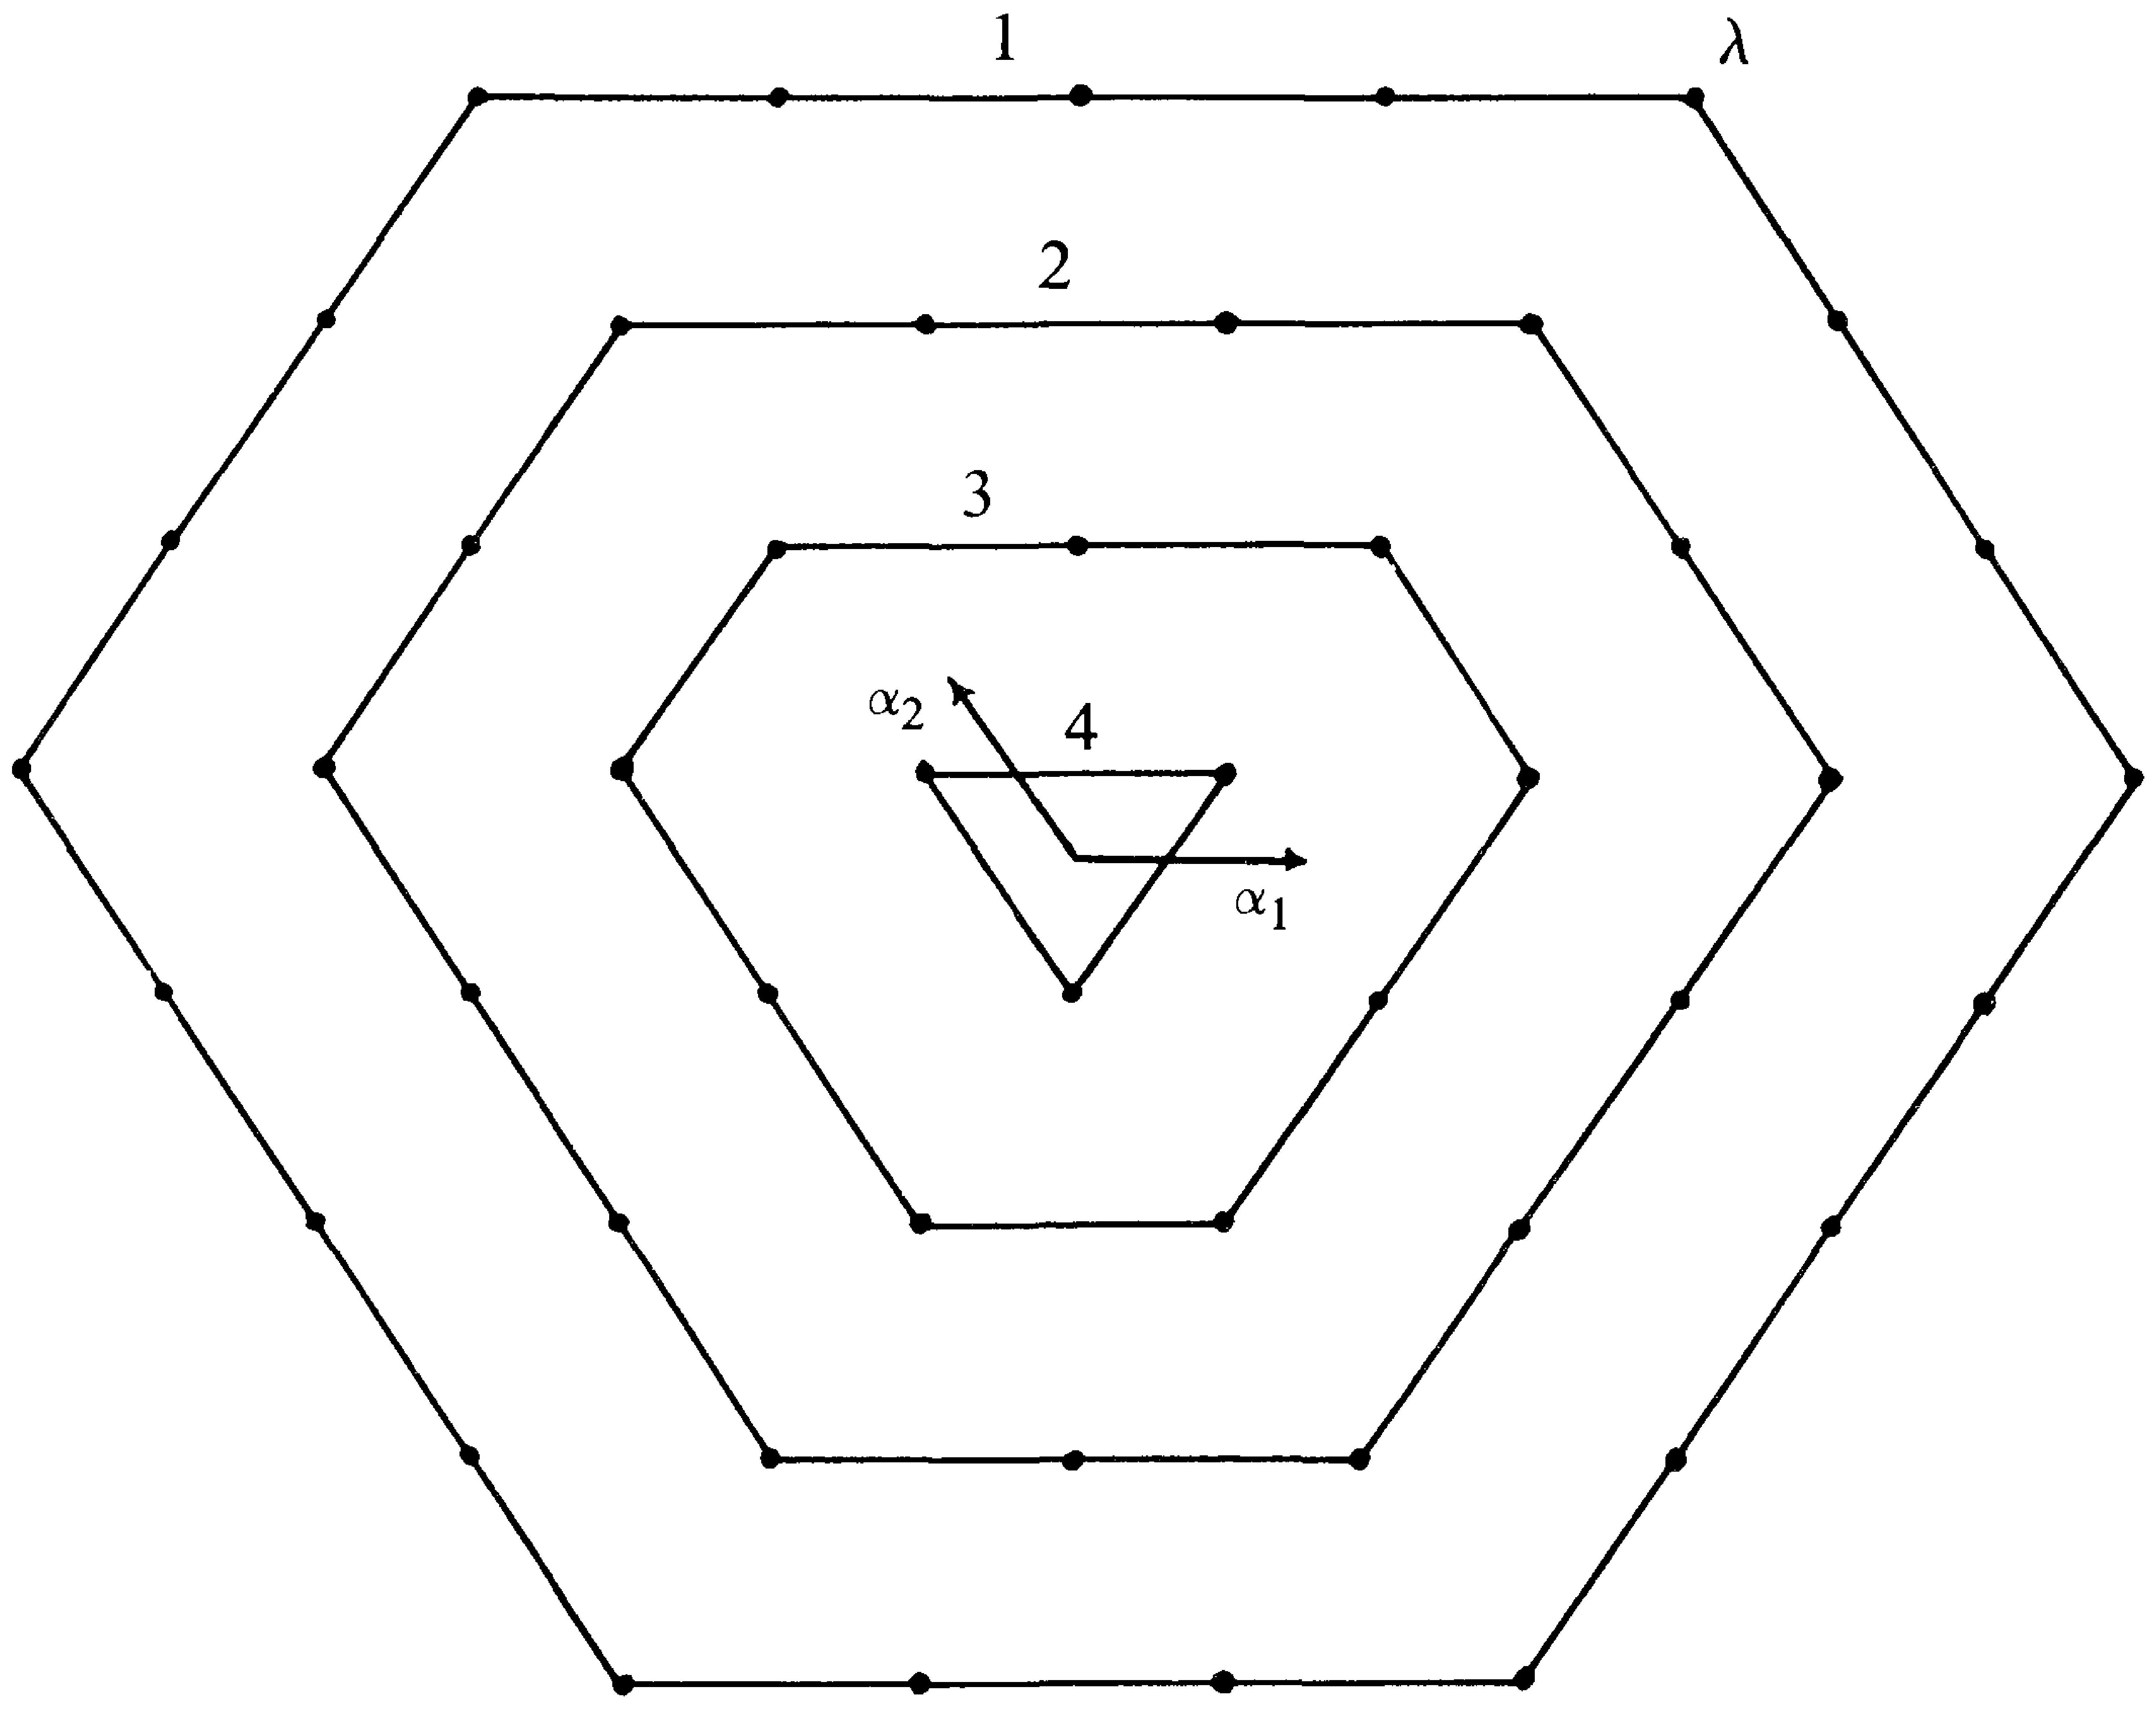
\includegraphics[max width=\textwidth, center]{2025_06_06_fac2836a92464059da43g-128}

Figure 1\\
fact about type $A_{2}$ (Antoine, Speiser [1]). For other root systems, the situation can be much more complicated; see $\S 22$ below for a more detailed discussion of multiplicities.

\subsection*{21.4. Generators and relations for $V(\lambda)$}
It is possible to describe more precisely the passage from $Z(\lambda)$ to its homomorphic image $V(\lambda)$, when $\lambda$ is dominant integral. This is not needed elsewhere in the text, but is of independent interest. In effect we shall rework some of the proof of Theorem 21.2.

Recall from (20.3) that $Z(\lambda)$ is isomorphic to $\mathfrak{U}(L) / I(\lambda)$, where $I(\lambda)$ is the left ideal of $\mathfrak{U}(L)$ generated by all $x_{\alpha}(\alpha>0)$, and by all $h_{\alpha}-\lambda\left(h_{\alpha}\right) \cdot 1(\alpha \in \Phi)$. Equivalently, $I(\lambda)$ is the annihilator of a maximal vector in $Z(\lambda)$. Now fix a dominant integral linear function $\lambda$, and let $J(\lambda)$ be the left ideal in $\mathfrak{U}(L)$ which annihilates a maximal vector of $V(\lambda)$. The inclusion $I(\lambda) \subset J(\lambda)$ induces the canonical map $Z(\lambda)=\mathfrak{U}(L) / I(\lambda) \rightarrow V(\lambda) \cong \mathfrak{U}(L) / J(\lambda)$. From the proof of Theorem 21.2 we recall that $y_{i}^{m_{i}+1} \in J(\lambda), 1 \leq i \leq \ell$, where $m_{i}=$ $\left\langle\lambda, \alpha_{i}\right\rangle$.

Theorem. Let $\lambda \in \Lambda^{+}, m_{i}=\left\langle\lambda, \alpha_{i}\right\rangle(1 \leq i \leq \ell)$. Then $J(\lambda)$ is generated by $I(\lambda)$ along with all $y_{i}^{m_{i}+1}(1 \leq i \leq \ell)$.

Proof. Suppose we can show that $V^{\prime}(\lambda)=\mathfrak{U}(L) / J^{\prime}(\lambda)$ is finite dimensional, where $J^{\prime}(\lambda)$ is the left ideal generated by $I(\lambda)$ along with all $y_{i}^{m_{i}+1}$. Since $V^{\prime}(\lambda)$ is standard cyclic (or 0), it must be irreducible (or 0) (Theorem 20.2(d), with Weyl's Theorem on complete reducibility). But $J^{\prime}(\lambda) \subset J(\lambda)$ implies that $V(\lambda)$ is a homomorphic image of $V^{\prime}(\lambda)$, forcing $V^{\prime}(\lambda) \cong V(\lambda)$, whence $J^{\prime}(\lambda)=J(\lambda)$ as desired.

To show that $V^{\prime}(\lambda)$ is finite dimensional, it would in turn suffice to show that it is a sum of finite dimensional $S_{i}$-submodules ( $1 \leq i \leq \ell$ ), because then the proof of Theorem 21.2 would go through exactly as before. For this it is enough to show that each $y_{i}$ is locally nilpotent on $V^{\prime}(\lambda)$ (this is of course obvious already for the $x_{i}$, since we cannot have $\mu+k \alpha_{i} \prec \lambda$ for all $k \geq 0$ ). By hypothesis, the coset of 1 in $V^{\prime}(\lambda)$ is killed by a suitable power of $y_{i}$ (namely, $m_{i}+1$ ). We know (Theorem 20.2) that $V^{\prime}(\lambda)$ is spanned by the cosets of all $y_{i_{1}} \ldots y_{i_{t}}\left(1 \leq i_{j} \leq \ell\right)$. The following lemma implies that if the coset of this monomial is killed (i.e. sent into $J^{\prime}(\lambda)$ ) by $y_{i}^{k}$, then the coset of the longer monomial $y_{i_{0}} y_{i_{1}} \ldots y_{i_{t}}$ is killed by $y_{i}^{k+3}$. Induction on length of monomials, starting at 1 , then proves the local nilpotence of $y_{i}$.

Lemma. Let $\mathfrak{A}$ be an associative algebra over $\mathrm{F}, y, z \in \mathfrak{A}$. Then $\left[y^{k}, z\right]=$ $\binom{k}{1}[y, z] y^{k-1}+\binom{k}{2}[y,[y, z]] y^{k-2}+\ldots+[y,[y, \ldots,[y, z] \ldots] \ldots]$.

Proof. Use induction on $k$, the case $k=1$ being the identity $[y, z]=$ $[y, z]$. The induction step is easy, and is left to the reader.

To apply the lemma, take $\mathfrak{N}$ to be $\mathfrak{U}(L)$, and take $y, z$ to be root vectors belonging to two negative roots. We know that $(\operatorname{ad} y)^{4}(z)=0$, since root strings have length at most 4 , so the identity obtained in the lemma reduces to: $\left[y^{k}, z\right]=k[y, z] y^{k-1}+\binom{k}{2}[y,[y, z]] y^{k-2}+\binom{k}{3}[y,[y,[y, z]]] y^{k-3}$.

\section*{Exercises}
\begin{enumerate}
  \item The reader can check that we have not yet used the simple transitivity of $\mathscr{W}$ on bases of $\Phi$ (Theorem 10.3(e)), only the transitivity. Use representation theory to obtain a new proof, as follows: There exists a finite dimensional irreducible module $V(\lambda)$ for which all $\langle\lambda, \alpha\rangle(\alpha \in \Delta)$ are distinct and positive. If $\sigma \in \mathscr{W}$ permutes $\Delta$, then $\sigma \lambda=\lambda$, forcing $\sigma=1$.
  \item Draw the weight diagram for the case $\mathrm{B}_{2}, \lambda=\lambda_{1}+\lambda_{2}$ (notation of Chapter III).
  \item Let $\lambda \in \Lambda^{+}$. Prove that 0 occurs as a weight of $V(\lambda)$ if and only if $\lambda$ is a sum of roots.
  \item Recall the module $Z(\lambda)$ constructed in (20.3). Use Lemma 21.2 to find certain maximal vectors in $Z(\lambda)$, when $\lambda \in \Lambda$ : the coset of $y_{i}^{m_{i}+1}$, $m_{i}=\left\langle\lambda, \alpha_{i}\right\rangle$, is a maximal vector provided $m_{i}$ is nonnegative (Cf. Exercise 7.7.)
  \item Let $V$ be a faithful finite dimensional $L$-module, $\Lambda(V)$ the subgroup of $\Lambda$ generated by the weights of $V$. Then $\Lambda(V) \supset \Lambda_{r}$. Show that every subgroup of $\Lambda$ including $\Lambda_{r}$ is of this type.
  \item If $V=V(\lambda), \lambda \in \Lambda^{+}$, prove that $V^{*}$ is isomorphic (as $L$-module) to $V(-\sigma \lambda)$, where $\sigma \in \mathscr{W}$ is the unique element of $\mathscr{W}$ sending $\Delta$ to $-\Delta$ (Exercise 10.9, cf. Exercise 13.5).
  \item Let $V=V(\lambda), W=V(\mu)$, with $\lambda, \mu \in \Lambda^{+}$. Prove that $\Pi(V \otimes W)=$ $\left\{\nu+\nu^{\prime} \mid \nu \in \Pi(\lambda), \nu^{\prime} \in \Pi(\mu)\right\}$ and that $\operatorname{dim}(V \otimes W)_{\nu+\nu^{\prime}}$ equals $\sum_{\pi+\pi^{\prime}=\nu+\nu^{\prime}} \operatorname{dim} V_{\pi} \cdot \operatorname{dim} W_{\pi^{\prime}}$\\
In particular, $\lambda+\mu$ occurs with multiplicity one, so $V(\lambda+\mu)$ occurs exactly once as a direct summand of $V \otimes W$.
  \item Let $\lambda_{1}, \ldots, \lambda_{\ell}$ be the fundamental dominant weights for the root system $\Phi$ of $L$ (13.1). Show how to construct an arbitrary $V(\lambda), \lambda \in \Lambda^{+}$, as a direct summand in a suitable tensor product of modules $V\left(\lambda_{1}\right), \ldots$, $V\left(\lambda_{\ell}\right)$ (repetitions allowed).
  \item Prove Lemma 21.4 and deduce Lemma 21.2 from it.
  \item Let $L=\mathfrak{s l}\left(\ell+1\right.$, F), with CSA $H=\mathfrak{d}(\ell+1$, F $) \cap L$. Let $\mu_{1}, \ldots, \mu_{\ell+1}$ be the coordinate functions on $H$, relative to the standard basis of $\mathfrak{g l}(\ell+1$, F). Then $\sum \mu_{i}=0$, and $\mu_{1}, \ldots, \mu_{\ell}$ form a basis of $H^{*}$, while the set of $\alpha_{i}=\mu_{i}-\mu_{i+1}(1 \leq i \leq \ell)$ is a base $\Delta$ for the root system $\Phi$. Verify that $\mathscr{W}$ acts on $H^{*}$ by permuting the $\mu_{i}$; in particular, the reflection with respect to $\alpha_{i}$ interchanges $\mu_{i}, \mu_{i+1}$ and leaves the other $\mu_{j}$ fixed. Then show that the fundamental dominant weights relative to $\Delta$ are given by $\lambda_{k}=\mu_{1}+\ldots+\mu_{k}(1 \leq k \leq \ell)$.
  \item Let $V=\mathrm{F}^{\ell+1}, L=\mathfrak{s l}(V)$. Fix the CSA $H$ and the base $\Delta=\left(\alpha_{1}, \ldots, \alpha_{\ell}\right)$ of $\Phi$ as in Exercise 10. The purpose of this exercise is to construct irreducible $L$-modules $V_{k}(1 \leq k \leq \ell)$ of highest weight $\lambda_{k}$.\\
(a) For $k=1, V_{1}=V$ is irreducible of highest weight $\lambda_{1}$.\\
(b) In the $k$-fold tensor product $V \otimes \ldots \otimes V, k \geq 2$, define $V_{k}$ to be the subspace of skew-symmetric tensors: If $\left(v_{1}, \ldots, v_{\ell+1}\right)$ is the canonical basis of $V, V_{k}$ has basis consisting of the $\binom{\ell+1}{k}$ vectors\\
(*)
\end{enumerate}

$$
\left[v_{i_{1}}, \ldots, v_{i_{k}}\right]=\sum_{\pi \in \mathscr{F}_{k}} \operatorname{sn}(\pi) v_{\pi\left(i_{1}\right)} \otimes \ldots \otimes v_{\pi\left(i_{k}\right)},
$$

where $i_{1}<i_{2}<\ldots<i_{k}$. Show that (*) is of weight $\mu_{i_{1}}+\ldots+\mu_{i_{k}}$.\\
(c) Prove that $L$ leaves the subspace $V_{k}$ invariant and that all the weights $\mu_{i_{1}}+\ldots+\mu_{i_{k}}\left(i_{1}<\ldots<i_{k}\right)$ are distinct and conjugate under $\mathscr{W}$. Conclude that $V_{k}$ is irreducible, of highest weight $\lambda_{k}$. (Cf. Exercise 13.13.)

\section*{Notes}
Theorem 21.4 is more or less well known; our treatment is based on an addendum to the thesis of Verma [1], cf. also Harish-Chandra [1]. Weight diagrams for $A_{2}$ appear in Antoine, Speiser [1]; see also Belinfante, Kolman [1], and Samelson [1].

\section*{22. Multiplicity formula}
All modules considered in this section are finite dimensional.\\
If $\mu \in H^{*}$ is an integral linear function, define the multiplicity of $\mu$ in $V(\lambda), \lambda \in \Lambda^{+}$, to be $m_{\lambda}(\mu)=\operatorname{dim} V(\lambda)_{\mu}$ ( $=0$ in case $\mu$ is not a weight of\\
$V(\lambda)$ ). When $\lambda$ is fixed we write simply $m(\mu)$. Our aim is to derive Freudenthal's recursion formula for $m_{\lambda}(\mu)$, by computing the trace of a Casimir-type element on $V(\lambda)_{\mu}$; using the fact that the element in question acts as a nonzero scalar on $V(\lambda)$, we can recover in this way $\operatorname{dim} V(\lambda)_{\mu}$.

\subsection*{22.1. A universal Casimir element}
Recall from (6.2) the notion of Casimir element $c_{\phi}$ of a representation of $L$, which was used to prove Weyl's Theorem on complete reducibility. Now that $\mathfrak{U}(L)$ is available we can make a "universal" construction of this sort.

Begin with the adjoint representation of $L$, whose trace form is just the Killing form $\kappa$. It is easy to deduce from $\S 8$ a natural construction of dual bases relative to $\kappa$. If $\alpha, \beta$ are arbitrary linear functions on $H$, we know that $L_{\alpha}$ is orthogonal to $L_{\beta}$ except when $\beta=-\alpha$ (Proposition 8.1). We also know that the restriction of $\kappa$ to $H$ is nondegenerate. Therefore we can proceed as follows. Choose any basis of $H$, say the standard one ( $h_{1}, \ldots, h_{\ell}$ ) (relative to $\Delta$ ), and let ( $k_{1}, \ldots, k_{\ell}$ ) be the dual basis of $H$, relative to the restriction of $\kappa$ to $H$. Next choose nonzero $x_{\alpha}$ in each $L_{\alpha}(\alpha \in \Phi)$, and let $z_{\alpha}$ be the (unique) element of $L_{-\alpha}$ satisfying $\kappa\left(x_{\alpha}, z_{\alpha}\right)=1$. By the remarks above, the bases $\left(h_{i}, 1 \leq i \leq \ell ; x_{\alpha}, \alpha \in \Phi\right)$ and $\left(k_{i}, 1 \leq i \leq \ell ; z_{\alpha}, \alpha \in \Phi\right)$ are dual relative to $\kappa$. $A$ word of caution, however: The pair $x_{\alpha}, z_{\alpha}$ must not be confused with our customary choice of $x_{\alpha}, y_{\alpha}$ such that $\left[x_{\alpha} y_{\alpha}\right]=h_{\alpha}$. Rather, we have here $\left[x_{\alpha} z_{\alpha}\right]=t_{\alpha}=[(\alpha, \alpha) / 2] h_{\alpha}$ (Proposition 8.3(c)).

By definition, a Casimir element for ad is the endomorphism of $L$ given by $c_{\text {ad }}=\sum_{i=1}^{\ell} \operatorname{ad} h_{\imath}$ ad $k_{i}+\sum_{\alpha \in \Phi} \operatorname{ad} x_{\alpha}$ ad $z_{\alpha}$. This construction might suggest to the reader consideration of the element $c_{L}=\sum_{i=1}^{\ell} h_{i} k_{i}+\sum_{\alpha \in \Phi} x_{\alpha} z_{\alpha} \in \mathfrak{U}(L)$. If ad is extended (uniquely) to a homomorphism of associative algebras ad: $\mathfrak{U}(L) \rightarrow$ End $L$, then ad $c_{L}$ is none other than $c_{\text {ad }}$. For this reason we call $c_{L}$ a universal Casimir element of $L$. It is not difficult to see that $c_{L}$ is independent of the choice of basis of $L$ (Exercise 2). The argument in (6.2) shows that for any representation $\phi$ of $L, \phi\left(c_{L}\right)$ commutes with $\phi(L)$, hence acts as a scalar if $\phi$ is irreducible.

Let us investigate how $\phi\left(c_{L}\right)$ is related to a Casimir element $c_{\phi}$. This is easy to see in case $L$ is simple, so we treat this case first (cf. Exercise 6.6).

Lemma. Let $L$ be a simple Lie algebra. If $f(x, y)$ and $g(x, y)$ are nondegenerate symmetric, associative bilinear forms on $L$, then there is a nonzero scalar a such that $f(x, y)=a g(x, y)$ for all $x, y \in L$.

Proof. Each form (being nondegenerate) sets up a natural vector space isomorphism of $L$ onto $L^{*}$, via $x \mapsto s$, where $s(y)=f(x, y)$ or $g(x, y)$. The associativity guarantees that these are actually isomorphisms of $L$-modules (recall from (6.1) how $L^{*}$ is made into an $L$-module). Combining one of these maps with the inverse of the other therefore sets up an $L$-module isomorphism $\pi: L \rightarrow L$. But $L$ is an irreducible $L$-module (being simple), so\\
$\pi$ is a scalar multiplication, thanks to Schur's Lemma. In other words, we have $0 \neq a \in \mathrm{~F}$ such that if $f(x, y)=g(z, y)$ (for all $y \in L$ ), then $z=a x$. $\square$

Let $\phi: L \rightarrow \mathfrak{g l}(V)$ be a representation of $L, L$ simple. If $\phi(L)=0$, everything is clear. Otherwise $\phi$ is faithful (since $\operatorname{Ker} \phi$ is an ideal of $L$ ), so the form $f(x, y)=\operatorname{Tr}(\phi(x) \phi(y))$ on $L$ is nondegenerate, as well as associative. The Killing form has the same properties, so it must be a nonzero multiple af (by the lemma). In particular, given one basis of $L$, the dual basis relative to $\kappa$ is gotten by multiplying the dual basis vectors relative to $f$ by $1 / a$. This shows that $\phi\left(c_{L}\right)=(1 / a) c_{\phi}$. In words, the ordinary Casimir element of $\phi$ is a nonzero multiple of the image of the universal Casimir element.

Finally, let $L$ be semisimple. We observed in (5.2) that distinct simple ideals of $L$ are orthogonal to each other, relative to $\kappa$. This makes it clear that the dual bases selected above can be chosen to be unions of analogous dual bases for the simple components of $L$ (relative to their Killing forms, which are gotten by restricting $\kappa$ ). Therefore $c_{L}=c_{L_{1}}+\cdots+c_{L_{t}}$ $\left(L=L_{1} \oplus \cdots \oplus L_{t}\right)$, and if $\phi$ is a representation of $L$, each $\phi\left(c_{L_{i}}\right)$ is proportional to the corresponding $c_{\phi_{i}}\left(\phi_{i}=\left.\phi\right|_{L_{i}}\right)$, where $\phi_{i}$ is either trivial or faithful for each $i$. So $\phi\left(c_{L}\right)$ is again very closely related, though not necessarily proportional, to $c_{\phi}$. In particular, this shows again that $\phi\left(c_{L}\right)$ commutes with $\phi(L)$. The precise value of the scalar by which $\phi\left(c_{L}\right)$ acts will be determined below, when $\phi$ is irreducible.

\subsection*{22.2. Traces on weight spaces}
Fix an irreducible $L$-module $V=V(\lambda), \lambda \in \Lambda^{+}$, and denote by $\phi$ the representation it affords. Fix also the dual bases of $L$ relative to $\kappa$ chosen in (22.1). In this subsection we are going to compute, for each weight $\mu$ of $V$, the trace on $V_{\mu}$ of the endomorphism $\phi\left(x_{\alpha}\right) \phi\left(z_{\alpha}\right)$. This makes sense, because $\phi\left(z_{\alpha}\right)$ maps $V_{\mu}$ into $V_{\mu-\alpha}$ and then $\phi\left(x_{\alpha}\right)$ maps $V_{\mu-\alpha}$ back into $V_{\mu}$.

Since we are working with only one root $\alpha$, we can utilize the representation theory of $S_{\alpha}(\S 7)$. Some modifications are needed, however, because our basis ( $x_{\alpha}, z_{\alpha}, t_{\alpha}$ ) is nonstandard; it is related to the standard basis ( $x_{\alpha}, y_{\alpha}, h_{\alpha}$ ) by $z_{\alpha}=[(\alpha, \alpha) / 2] y_{\alpha}, t_{\alpha}=[(\alpha, \alpha) / 2] h_{\alpha}$. Let $\left(v_{0}, v_{1}, \ldots, v_{m}\right)$ be the basis used in formulas (a)-(c), Lemma 7.2, for the irreducible $S_{\alpha}$-module of highest weight $m$. It will be convenient to replace this basis by ( $w_{0}, \ldots, w_{m}$ ), where $w_{i}=i!\left[(\alpha, \alpha)^{i} / 2^{i}\right] v_{i}$. After making this substitution, we obtain:\\
(a') $t_{\alpha \cdot} w_{i}=(m-2 i)[(\alpha, \alpha) / 2] w_{i}$;\\
(b') $z_{\alpha} \cdot w_{i}=w_{i+1}, \quad\left(w_{m+1}=0\right)$;\\
(c') $x_{\alpha} \cdot w_{i}=i(m-i+1)[(\alpha, \alpha) / 2] w_{i-1}, \quad\left(w_{-1}=0\right)$.\\
Therefore:


\begin{equation*}
x_{\alpha} z_{\alpha} \cdot w_{i}=(m-i)(i+1)[(\alpha, \alpha) / 2] w_{i} . \tag{1}
\end{equation*}


Now let $\mu$ be any weight of $V$ for which $\mu+\alpha$ is not a weight. Then (21.3) the $\alpha$-string of weights through $\mu$ consists of $\mu, \mu-\alpha, \ldots, \mu-m \alpha$, where\\
$m=\langle\mu, \alpha\rangle$. We keep $\mu, \alpha, m$ fixed throughout the following discussion. The representation of $S_{\alpha}$ on the sum of weight spaces $W=V_{\mu}+V_{\mu-\alpha}+\ldots+$ $V_{\mu-m \alpha}$ is a direct sum of irreducible representations (Weyl's Theorem), each involving a string of weights stable under $\sigma_{\alpha}$. To be more precise, let $n_{i}$ ( $0 \leq i \leq[m / 2]$ ) denote the number of such constituents having highest weight $(\mu-i \alpha)\left(h_{\alpha}\right)$. Then $m(\mu-i \alpha)=n_{0}+\ldots+n_{i}$, and in turn, $n_{i}=m(\mu-i \alpha)$ $-m(\mu-(i-1) \alpha)$. This is shown schematically in Figure 1, for the case $m$ even.\\
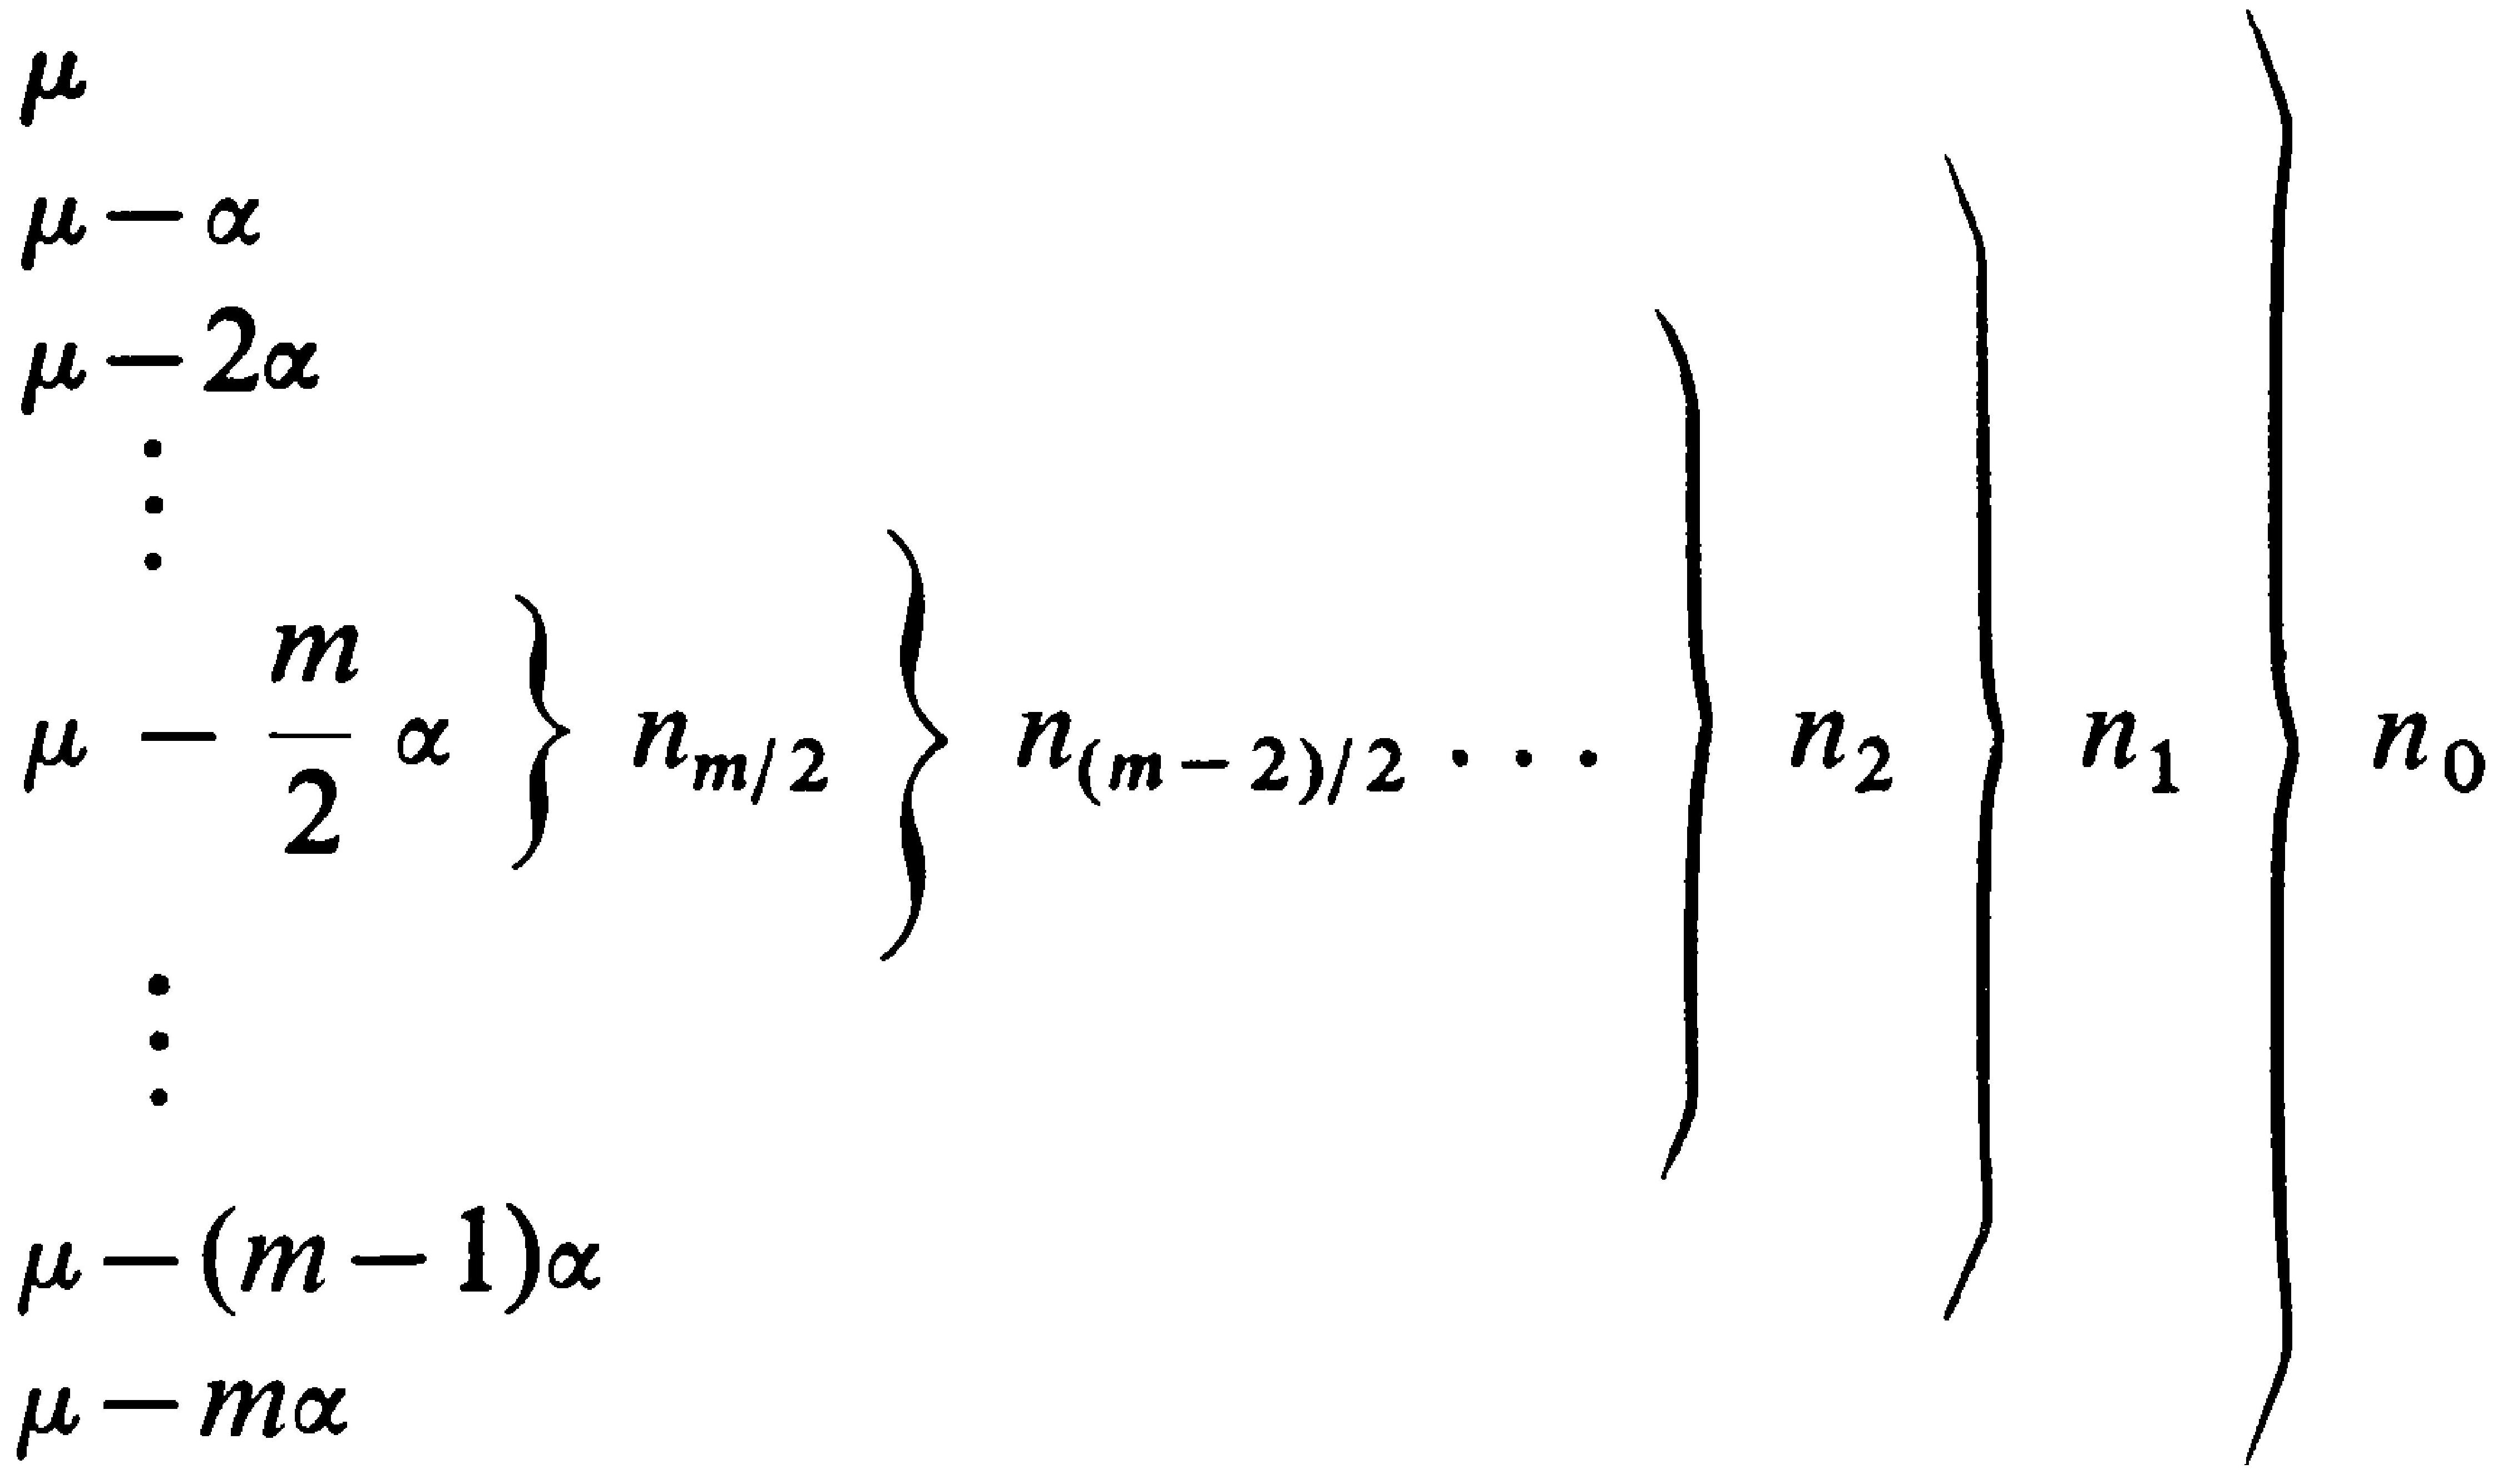
\includegraphics[max width=\textwidth, center]{2025_06_06_fac2836a92464059da43g-133}

Figure 1. ( $m$ even)\\
For each fixed $k, 0 \leq k \leq m / 2$, we want to calculate the trace of $\phi\left(x_{\alpha}\right) \phi\left(z_{\alpha}\right)$ on $V_{\mu-k x}$. Let $0 \leq i \leq k$. In a typical irreducible $S_{\alpha}$-summand of $W$ having highest weight $m-2 i=(\mu-i \alpha)\left(h_{\alpha}\right)$, the weight space corresponding to $\mu-k \alpha$ is spanned by the vector $w_{k-i}$ (in the above notation). Replacing $m$ by $m-2 i$ and $i$ by $k-i$ in formula (1), we obtain:


\begin{equation*}
\phi\left(x_{\alpha}\right) \phi\left(z_{\alpha}\right) w_{k-i}=(m-i-k)(k-i+1)[(\alpha, \alpha) / 2] w_{k-i} . \tag{2}
\end{equation*}


There are $n_{i} S_{\alpha}$-summands of $W$ having highest weight $m-2 i$, so the matrix of $\phi\left(x_{\alpha}\right) \phi\left(z_{\alpha}\right)$ (restricted to $V_{\mu-k \alpha}$ ) has $n_{i}$ diagonal entries of the form given by (2), relative to a suitable basis of eigenvectors. Letting $i$ range from 0 to $k$, we obtain for $\phi\left(x_{\alpha}\right) \phi\left(z_{\alpha}\right)$ a diagonal matrix of order $m(\mu-k \alpha)=n_{0}$ $+\ldots+n_{k}$, with trace:


\begin{align*}
& \sum_{i=0}^{k} n_{i}(m-i-k)(k-i+1)(\alpha, \alpha) / 2  \tag{3}\\
= & \sum_{i=0}^{k}(m(\mu-i \alpha)-m(\mu-(i-1) \alpha))(m-i-k)(k-i+1)(\alpha, \alpha) / 2 \\
= & \sum_{i=0}^{k} m(\mu-i \alpha)(m-2 i)(\alpha, \alpha) / 2 .
\end{align*}


The last equality follows, because the coefficient of $m(\mu-i \alpha)$ is $(\alpha, \alpha) / 2$ times $(m-i-k)(k-i+1)-(m-i-k-1)(k-i)=m-2 i$. (The reader should check directly the extreme case $i=k$.) Now recall that $m / 2=(\mu, \alpha) /(\alpha, \alpha)$. So (3) becomes:


\begin{equation*}
\operatorname{Tr}_{V_{\mu-k \alpha}} \phi\left(x_{\alpha}\right) \phi\left(z_{\alpha}\right)=\sum_{i=0}^{k} m(\mu-i \alpha)(\mu-i \alpha, \alpha) . \tag{4}
\end{equation*}


This takes care of the weights $\mu-k \alpha$ in the top half of the "ladder" (Figure 1). Since the reflection $\sigma_{\alpha}$ interchanges top and bottom, we can expect similar behavior; in particular, $m(\mu-i \alpha)=m(\mu-(m-i) \alpha)$ for $m / 2<i \leq m$. Imitating the above reasoning for fixed $k, m / 2<k \leq m$, we get:


\begin{equation*}
\operatorname{Tr}_{V_{\mu-k \alpha}} \phi\left(x_{\alpha}\right) \phi\left(z_{\alpha}\right)=\sum_{i=0}^{m-k-1} m(\mu-i \alpha)(\mu-i \alpha, \alpha) . \tag{5}
\end{equation*}


(We should sum to $m-k$, but $\phi\left(z_{\alpha}\right)$ kills a vector of weight $\mu-k \alpha$ belonging to an $S_{\alpha}$-summand of $W$ having highest weight $\mu-(m-k) \alpha$.)

But notice that, for $m / 2<i \leq m,(\mu-i \alpha, \alpha)+(\mu-(m-i) \alpha, \alpha)=(2 \mu-m \alpha$, $\alpha)=0$, because $m=2(\mu, \alpha) /(\alpha, \alpha)$. Therefore:


\begin{equation*}
m(\mu-i \alpha)(\mu-i \alpha, \alpha)+m(\mu-(m-i) \alpha)(\mu-(m-i) \alpha, \alpha)=0 . \tag{6}
\end{equation*}


This shows that certain pairs of summands may be added to (5): $k+1$ and $m-(k+1), k+2$ and $m-(k+2)$, etc. (Note that for $m=2 i$ even, (6) forces $(\mu-i \alpha, \alpha)=0$.) In other words, (5) reduces to (4), for arbitrary $k$.

Finally, if we wish to consider an arbitrary weight $\nu$ of $V$, we form the $\alpha$-string through $\nu$ and let the final term $\nu+k \alpha$ play the role of $\mu$ in the above formulas. With $m(\mu)=0$ for all $\mu$ such that $V_{\mu}=0$, a little juggling then permits us to rewrite (4) as follows, for arbitrary $\mu \in \Pi(\lambda)$ :


\begin{equation*}
\operatorname{Tr}_{V_{\mu}} \phi\left(x_{\alpha}\right) \phi\left(z_{\alpha}\right)=\sum_{i=0}^{\infty} m(\mu+i \alpha)(\mu+i \alpha, \alpha) . \tag{7}
\end{equation*}


\subsection*{22.3. Freudenthal's formula}
Let $\phi, V$ be as in (22.2), $\operatorname{dim} V>1$. Recall from (22.1) the universal Casimir element $c_{L}=\sum_{i=1}^{\ell} h_{i} k_{i}+\sum_{\alpha \in \Phi} x_{\alpha} z_{\alpha}$. Since $\phi$ is irreducible, $\phi\left(c_{L}\right)$ is multiplication by a scalar, say $c$. Fix a weight $\mu$ of $V$. We want to calculate $\operatorname{Tr}_{V_{\mu}} \phi\left(c_{L}\right)=$ $c m(\mu)$.

First of all, $\phi\left(h_{i}\right)$ is just scalar multiplication by $\mu\left(h_{i}\right)$ in $V_{\mu}$, and similarly for $\phi\left(k_{i}\right)$. Let $t_{\mu} \in H$ satisfy $\mu(h)=\kappa\left(t_{\mu}, h\right)$ for all $h \in H$ (as in §8). Write $t_{\mu}=\sum_{i} a_{i} h_{i}$; then by definition $\mu\left(h_{i}\right)=\sum_{j} a_{j} \kappa\left(h_{j}, h_{i}\right)$ and $\mu\left(k_{i}\right)=\sum_{j} a_{j} \kappa\left(h_{j}\right.$, $\left.k_{i}\right)=a_{i}($ by duality $)$. Therefore, $(\mu, \mu)=\sum_{i, j} a_{i} a_{j} \kappa\left(h_{j}, h_{i}\right)=\sum_{i} \mu\left(h_{i}\right) \mu\left(k_{i}\right)$, whence:


\begin{equation*}
\sum_{i} \operatorname{Tr}_{V_{\mu}} \phi\left(h_{i}\right) \phi\left(k_{i}\right)=m(\mu)(\mu, \mu) \tag{8}
\end{equation*}


Combining (8) with formula (7) in (22.2), we have:


\begin{equation*}
c m(\mu)=(\mu, \mu) m(\mu)+\sum_{\alpha \in \Phi} \sum_{i=0}^{\infty} m(\mu+i \alpha)(\mu+i \alpha, \alpha) \tag{9}
\end{equation*}


Notice that the terms $m(\mu)(\mu, \alpha)$ and $m(\mu)(\mu,-\alpha)$ both occur (and cancel), so we can omit the index $i=0$.

We claim that formula (9) remains valid for arbitrary $\mu \in \Lambda, \mu \notin \Pi(\lambda)$, in which case it reads: $0=\sum_{\alpha \in \Phi} \sum_{i=1}^{\infty} m(\mu+i \alpha)(\mu+i \alpha, \alpha)$. Indeed, if $\mu \notin \Pi(\lambda)$,\\
then for each $\alpha \in \Phi$ the weights (if any) of the form $\mu+i \alpha$ must occur in a string with all $i$ positive or all $i$ negative. In the latter case, the summand for $\alpha$ is 0 ; in the former case this is equally true, by an argument analogous to that in (22.2) for formula (6).

The preceding discussion actually shows that for each fixed $\alpha \in \Phi$ and each $\mu \in \Lambda$, we have:


\begin{equation*}
\sum_{i=-\infty}^{\infty} m(\mu+i \alpha)(\mu+i \alpha, \alpha)=0 . \tag{10}
\end{equation*}


In particular,


\begin{equation*}
\sum_{i=1}^{\infty} m(\mu-i \alpha)(\mu-i \alpha,-\alpha)=m(\mu)(\mu, \alpha)+\sum_{i=1}^{\infty} m(\mu+i \alpha)(\mu+i \alpha, \alpha) . \tag{11}
\end{equation*}


Substituting (11) in (9) (summation starting with $i=1$, as remarked following (9)), we obtain finally:


\begin{align*}
c m(\mu)=(\mu, \mu) m(\mu) & +\sum_{\alpha \succ 0} m(\mu)(\mu, \alpha)  \tag{12}\\
& +2 \sum_{\alpha \succ 0} \sum_{i=1}^{\infty} m(\mu+i \alpha)(\mu+i \alpha, \alpha) .
\end{align*}


Letting $\delta=(1 / 2) \sum_{\alpha \succ 0} \alpha(13.3)$, this can be rewritten as:


\begin{equation*}
c m(\mu)=(\mu, \mu+2 \delta) m(\mu)+2 \sum_{\alpha \succ 0} \sum_{i=1}^{\infty} m(\mu+i \alpha)(\mu+i \alpha, \alpha) . \tag{13}
\end{equation*}


The only drawback to this formula is that it still involves $c$. But there is a special case in which we know $m(\mu)$, namely: $m(\lambda)=1$. Moreover, $m(\lambda+i \alpha)$ $=0$ for all positive roots $\alpha$, all $i \geq 1$. Accordingly, we can solve (13) for the value $c=(\lambda, \lambda+2 \delta)=(\lambda+\delta, \lambda+\delta)-(\delta, \delta)$. (Actually, it is not hard to compute $c$ directly: Exercise 23.4.) These results may now be summarized in Freudenthal's formula.

Theorem. Let $V=V(\lambda)$ be an irreducible L-module of highest weight $\lambda$, $\lambda \in \Lambda^{+}$. If $\mu \in \Lambda$, then the multiplicity $m(\mu)$ of $\mu$ in $V$ is given recursively as follows:


\begin{equation*}
((\lambda+\delta, \lambda+\delta)-(\mu+\delta, \mu+\delta)) m(\mu)=2 \sum_{\alpha \succ 0} \sum_{i=1}^{\infty} m(\mu+i \alpha)(\mu+i \alpha, \alpha) . \tag{14}
\end{equation*}


It still has to be observed that Freudenthal's formula provides an effective method for calculating multiplicities, starting with $m(\lambda)=1$. Thanks to Proposition 21.3, Lemma C of (13.4) shows that for $\mu \in \Pi(\lambda), \mu \neq \lambda$, the quantity $(\lambda+\delta, \lambda+\delta)-(\mu+\delta, \mu+\delta)$ is nonzero; so $m(\mu)=0$ whenever this quantity is $0, \mu \neq \lambda$. Therefore $m(\mu)$ is known provided all $m(\mu+i \alpha)(i \geq 1$, $\alpha \succ 0$ ) are known, i.e., provided all $m(\nu), \mu \underset{\neq}{\prec} \prec \lambda$, are known. (Some concrete examples will be given below.)

In practice, the use of Freudenthal's formula can be made more efficient by exploiting the fact that weights conjugate under the Weyl group have the\\
same multiplicity (Theorem 21.2). There exist computer programs for carrying out the calculations involved. Notice that the inner product can be normalized in any convenient way, since $m(\mu)$ appears as a quotient.

\subsection*{22.4. Examples}
To use Freudenthal's formula in any given case, we have to be able to compute explicitly the bilinear form on $\Lambda$. The form used above was the "natural" one (dual to the Killing form), but it may be normalized by any convenient scalar multiplication in view of the above remarks. One popular procedure is to require that all squared root lengths be 1,2 , or 3 , the smallest being 1 (for each irreducible component of $\Phi$ ). Alternatively, the inner product used in the construction of root systems in §12 can be chosen.

Example 1. $L=\mathfrak{s l}(3, \mathfrak{F}), \Phi=\left\{ \pm \alpha_{1}, \pm \alpha_{2}, \pm\left(\alpha_{1}+\alpha_{2}\right)\right\}, \Delta=\left\{\alpha_{1}, \alpha_{2}\right\}$, $\alpha_{1}=2 \lambda_{1}-\lambda_{2}, \alpha_{2}=-\lambda_{1}+2 \lambda_{2}, \lambda_{1}=(1 / 3)\left(2 \alpha_{1}+\alpha_{2}\right), \lambda_{2}=(1 / 3)\left(\alpha_{1}+2 \alpha_{2}\right)$. Require $\left(\alpha_{i}, \alpha_{i}\right)=1$, so that $\left(\alpha_{1}, \alpha_{2}\right)=-1 / 2,\left(\lambda_{i}, \lambda_{i}\right)=1 / 3$, and $\left(\lambda_{1}, \lambda_{2}\right)=$ $1 / 6$. Set $\lambda=\lambda_{1}+3 \lambda_{2}$. Then Freudenthal's formula yields the list of multiplicities in Table 1. Other data are listed also, for the reader's convenience. Weights are grouped by "level": calculation of $m(\mu)$ requires data only from higher levels. The reader should draw a weight diagram, in the manner of Figure 1 of (21.3).

Table 1.

\begin{center}
\begin{tabular}{|l|l|l|l|}
\hline
$\mu$ & $m(\mu)$ & ( $\mu+\delta, \mu+\delta$ ) & $\mu=m_{1} \lambda_{1}+m_{2} \lambda_{2}$ \\
\hline
$\{\lambda$ & 1 & 28/3 & $\lambda_{1}+3 \lambda_{2}$ \\
\hline
$\left\{\begin{array}{l}\lambda-\alpha_{1} \\ \lambda-\alpha_{2}\end{array}\right.$ & 1 & 25/3 & $-\lambda_{1}+4 \lambda_{2}$ \\
\hline
$\left\{\begin{array}{l}\lambda-\alpha_{1}-\alpha_{2} \\ \lambda-2 \alpha_{2}\end{array}\right.$ & 2 & 13/3 & $3 \lambda_{1}-\lambda_{2}$ \\
\hline
$\left\{\begin{array}{l}\lambda-\alpha_{1}-2 \alpha_{2} \\ \lambda-2 \alpha_{1}-\alpha_{2} \\ \lambda-3 \alpha_{2}\end{array}\right.$ & 2 &  &  \\
\hline
$\left\{\begin{array}{l}\lambda-2 \alpha_{1}-2 \alpha_{2} \\ \lambda-\alpha_{1}-3 \alpha_{2}\end{array}\right.$ & 2 & 4/3 & $2 \lambda_{1}-2 \lambda_{2}$ \\
\hline
$\left\{\begin{array}{l}\lambda-\alpha_{1}-4 \alpha_{2} \\ \lambda-2 \alpha_{1}-3 \alpha_{2} \\ \lambda-3 \alpha_{1}-2 \alpha_{2}\end{array}\right.$ & 2 & 13/3 & $-3 \lambda_{1}+2 \lambda_{2}$ \\
\hline
$\left\{\begin{array}{l}\lambda-2 \alpha_{1}-4 \alpha_{2} \\ \lambda-3 \alpha_{1}-3 \alpha_{2}\end{array}\right.$ & 1 & 4/3 & $\lambda_{1}-3 \lambda_{2}$ \\
\hline
$\left\{\begin{array}{l}\lambda-3 \alpha_{1}-4 \alpha_{2} \\ \lambda-4 \alpha_{1}-3 \alpha_{2}\end{array}\right.$ & 1 & 1/3 & $-4 \lambda_{1}+\lambda_{2}$ \\
\hline
$\left\{\lambda-4 \alpha_{1}-4 \alpha_{2}\right.$ & 1 & 4/3 & $-3 \lambda_{1}-\lambda_{2}$ \\
\hline
\end{tabular}
\end{center}

Example 2. Let $L$ be the simple algebra of type $\mathrm{G}_{2}$. The root system of $L$ is constructed explicitly in (12.1). Recall that $\alpha_{1}$ is short and $\alpha_{2}$ is long, so that $\lambda_{1}=2 \alpha_{1}+\alpha_{2}, \lambda_{2}=3 \alpha_{1}+2 \alpha_{2}$. Some information obtained by using Freudenthal's formula is listed in Table 2. The weight $m_{1} \lambda_{1}+m_{2} \lambda_{2}$ is abbreviated there by $m_{1} m_{2}$. Rows are indexed by highest weights $\lambda$, columns by dominant weights $\mu$, and the intersection of row $\lambda$ with column $\mu$ contains the integer $m_{\lambda}(\mu)$ (when this is nonzero). The reader should verify parts of the table for himself.

Table 2.

\begin{center}
\begin{tabular}{|l|l|l|l|l|l|l|l|l|l|l|l|l|l|l|}
\hline
 & 00 & 10 & 01 & 20 & 11 & 30 & 02 & 21 & 40 & 12 & 31 & 50 & 03 & 22 \\
\hline
00 & 1 &  &  &  &  &  &  &  &  &  &  &  &  &  \\
\hline
10 & 1 & 1 &  &  &  &  &  &  &  &  &  &  &  &  \\
\hline
01 & 2 & 1 & 1 &  &  &  &  &  &  &  &  &  &  &  \\
\hline
20 & 3 & 2 & 1 & 1 &  &  &  &  &  &  &  &  &  &  \\
\hline
11 & 4 & 4 & 2 & 2 & 1 &  &  &  &  &  &  &  &  &  \\
\hline
30 & 5 & 4 & 3 & 2 & 1 & 1 &  &  &  &  &  &  &  &  \\
\hline
02 & 5 & 3 & 3 & 2 & 1 & 1 & 1 &  &  &  &  &  &  &  \\
\hline
21 & 9 & 8 & 6 & 5 & 3 & 2 & 1 & 1 &  &  &  &  &  &  \\
\hline
40 & 8 & 7 & 5 & 5 & 3 & 2 & 1 & 1 & 1 &  &  &  &  &  \\
\hline
12 & 10 & 10 & 7 & 7 & 5 & 3 & 2 & 2 & 1 & 1 &  &  &  &  \\
\hline
31 & 16 & 14 & 12 & 10 & 7 & 6 & 4 & 3 & 2 & 1 & 1 &  &  &  \\
\hline
50 & 12 & 11 & 9 & 8 & 6 & 5 & 3 & 3 & 2 & 1 & 1 & 1 &  &  \\
\hline
03 & 9 & 7 & 7 & 5 & 4 & 4 & 3 & 2 & 1 & 1 & 1 & 0 & 1 &  \\
\hline
22 & 21 & 19 & 16 & 15 & 11 & 9 & 7 & 6 & 4 & 3 & 2 & 1 & 1 & 1 \\
\hline
\end{tabular}
\end{center}

\subsection*{22.5. Formal characters}
Let $\Lambda \subset H^{*}$ be, as before, the lattice of integral linear functions. If $V=V(\lambda), \lambda \in \Lambda^{+}$, we want to consider a formal sum of the weights $\mu \in \Pi(\lambda)$, each $\mu$ occurring in the sum $m(\mu)$ times. However, " $\mu+\nu$ " would be a poor notation to use in such a formal sum, since this already has a concrete meaning in $\Lambda$. Therefore we introduce the group ring of $\Lambda$ over $\mathbf{Z}$, denoted $\mathbf{Z}[\Lambda]$. By definition, $\mathbf{Z}[\Lambda]$ is a free $\mathbf{Z}$-module with basis elements $e(\lambda)$ in one-one correspondence with the elements $\lambda$ of $\Lambda$, with the addition denoted $e(\lambda)+$ $e(\mu) . \mathbf{Z}[\Lambda]$ becomes a commutative ring if we decree that $e(\lambda) e(\mu)=e(\lambda+\mu)$ and extend by linearity. (There is an identity element: $e(0)$.) $\mathscr{W}$ acts naturally on $\mathbf{Z}[\Lambda]$, by permuting the $e(\lambda): \sigma e(\lambda)=e(\sigma \lambda)$.

Now it makes good sense to define the formal character $c h_{V(\lambda)}$, or just $c h_{\lambda}$, of $V(\lambda)$ as the element $\sum_{\mu \in \Pi(\lambda)} m_{\lambda}(\mu) e(\mu)$ of $\mathbf{Z}[\Lambda]$. (Since $m_{\lambda}(\mu)=0$ whenever $\mu \notin \Pi(\lambda)$, we can even extend the summation to all $\mu \in \Lambda$.) For example, if $L=\mathfrak{s l}(2, \mathrm{~F})$, the formal character of $V(\lambda)$ is given by $c h_{\lambda}=e(\lambda)+e(\lambda-\alpha)$ $+e(\lambda-2 \alpha)+\ldots+e(\lambda-m \alpha), m=\langle\lambda, \alpha\rangle$. More generally, if $V$ is an arbitrary (finite dimensional) $L$-module, there is an essentially unique decomposition $V=V\left(\lambda_{1}\right) \oplus \ldots \oplus V\left(\lambda_{t}\right), \lambda_{i} \in \Lambda^{+}$, thanks to Weyl's Theorem and the classification theory (§21). So $c h_{V}=\sum_{i=1}^{t} c h_{\lambda_{i}}$ may be called the formal charac-\\
ter of $V$. Notice that each $\sigma \in \mathscr{W}$ fixes $c h_{V}$, since $\sigma$ permutes weight spaces in each irreducible summand of $V$ (Theorem 21.2).

Knowledge of $c h_{V}$ actually enables us to recover the irreducible constituents of $V$, because of the following result.

Proposition A. Let $f=\sum_{\lambda \in \Lambda} c(\lambda) e(\lambda), c(\lambda) \in \mathbf{Z}$, be fixed by all elements of $\mathscr{W}$.\\
Then $f$ can be written in one and only one way as a $\mathbf{Z}$-linear combination of the $c h_{\lambda}\left(\lambda \in \Lambda^{+}\right)$.

Proof. It is clear that $f=\sum_{\lambda \in \Lambda^{+}} c(\lambda)\left(\sum_{\sigma \in \mathscr{W}} e(\sigma \lambda)\right)$. For each $\lambda \in \Lambda^{+}$such that $c(\lambda) \neq 0$, the set of dominant $\mu \prec \lambda$ is finite (Lemma B of (13.2)). Let $M_{f}$ be the totality of such $\mu$ (for all such $\lambda$ ), so $M_{f}$ is finite. Let $\lambda \in \Lambda^{+}$be maximal among the $\lambda \in \Lambda^{+}$for which $c(\lambda) \neq 0$, and set $f^{\prime}=f-c(\lambda) c h_{\lambda}$, so clearly $f^{\prime}$ again satisfies the hypothesis of the proposition. We know that the dominant $\mu$ figuring in $c h_{\lambda}$ all satisfy $\mu \prec \lambda$, so they all lie in $M_{f}$. This shows that $M_{f^{\prime}} \subset M_{f}$. The inclusion is proper, because $\lambda \notin M_{f^{\prime}}$. By induction on Card ( $M_{f}$ ), we can write $f^{\prime}$ in the desired form; then $f$ also has the desired form. To start the induction, notice that the case Card $\left(M_{f}\right)=1$ is trivial: In this case a minimal dominant weight $\lambda$ is the only dominant weight figuring in $f$, whence $f=c(\lambda) c h_{\lambda}$, where $c h_{\lambda}=\sum_{\sigma \in \mathscr{V}} e(\sigma \lambda)$. The uniqueness assertion is left to the reader (Exercise 8).

One advantage in being able to multiply formal characters is brought out next.

Proposition B. Let $V, W$ be (finite dimensional) L-modules. Then ch $_{V \otimes W}=$ $c h_{V} . c h_{W}$.

Proof. On the one hand, from the way in which the action of $L$ on $V \otimes W$ is defined (6.1), it is clear that the weights of $V \otimes W$ are those of the form $\lambda+\mu(\lambda$ a weight of $V, \mu$ of $W)$, each occurring with multiplicity

$$
\sum_{\pi+\pi^{\prime}=\lambda+\mu} m_{V}(\pi) m_{W}\left(\pi^{\prime}\right)
$$

(cf. Exercise 21.7). But this is also what we get if we formally multiply $c h_{V}$ by $c h_{W}$. $\square$

\section*{Exercises}
\begin{enumerate}
  \item Let $\lambda \in \Lambda^{+}$. Prove, without using Freudenthal's formula, that $m_{\lambda}(\lambda-k \alpha)$ $=1$ for $\alpha \in \Delta$ and $0 \leq k \leq\langle\lambda, \alpha\rangle$.
  \item Prove that $c_{L}$ is in the center of $\mathfrak{U}(L)$ (cf. (23.2)). [Imitate the calculation in (6.2), with $\phi$ omitted.] Show also that $c_{L}$ is independent of the basis chosen for $L$.
  \item In Example 1 (22.4), determine the $\mathscr{W}$-orbits of weights, thereby verifying directly that $\mathscr{W}$-conjugate weights have the same multiplicity (cf. Theorem 21.2). [Cf. Exercise 13.12.]
  \item Verify the multiplicities shown in Figure 1 of (21.3).
  \item Use Freudenthal's formula and the data for $A_{2}$ in Example 1 (22.4) to compute multiplicities for $V(\lambda), \lambda=2 \lambda_{1}+2 \lambda_{2}$. Verify in particular that $\operatorname{dim} V(\lambda)=27$ and that the weight 0 occurs with multiplicity 3 . Draw the weight diagram.
  \item For $L$ of type $\mathrm{G}_{2}$, use Table 2 of (22.4) to determine all weights and their multiplicities for $V(\lambda), \lambda=\lambda_{1}+2 \lambda_{2}$. Compute $\operatorname{dim} V(\lambda)=286$. [Cf. Exercise 13.12.]
  \item Let $L=\mathfrak{s l}(2, \mathrm{~F})$, and identify $m \lambda_{1}$ with the integer $m$. Use Propositions A and B of (22.5), along with Theorem 7.2, to derive the Clebsch-Gordan formula: If $n \leq m$, then $V(m) \otimes V(n) \cong V(m+n) \oplus V(m+n-2) \oplus \ldots$ $\oplus V(m-n), n+1$ summands in all. (Cf. Exercise 7.6.)
  \item Prove the uniqueness part of Proposition 22.5A.
\end{enumerate}

\section*{Notes}
The proof of Freudenthal's formula is taken from Jacobson [1]; see also Freudenthal [1] and Freudenthal-de Vries [1]. For computational aspects, cf. Agrawala, Belinfante [1], Beck, Kolman [1], Krusemeyer [1], Burgoyne, Williamson [1]. A different algorithm has been found by Demazure [1]. The data in Table 2 is taken from Springer [1].

\section*{23. Characters}
Our object is to prove a theorem of Harish-Chandra on "characters" associated with the infinite dimensional modules $Z(\lambda), \lambda \in H^{*}$ (20.3). This theorem will be used in $\S 24$ to obtain a simple algebraic proof of Weyl's classical result on characters of finite dimensional modules. As a preliminary (which is also of independent interest) we shall prove in (23.1) a theorem of Chevalley on "lifting" invariants. None of this depends on Freudenthal's formula (22.3).

\subsection*{23.1. Invariant polynomial functions}
If $V$ is a finite dimensional vector space, the symmetric algebra $\mathfrak{S}\left(V^{*}\right)$ (see (17.1)) is called the algebra of polynomial functions on $V$, and is denoted $\mathfrak{B}(V)$. When a fixed basis $\left(f_{1}, \ldots, f_{n}\right)$ of $V^{*}$ is given, $\mathfrak{B}(V)$ becomes identified with the algebra of polynomials in $n$ variables $f_{1}, \ldots, f_{n}$. In this subsection we consider $\mathfrak{B}(L)$ and $\mathfrak{B}(H)$.

Since the weight lattice $\Lambda$ spans $H^{*}$, the polynomials in the $\lambda \in \Lambda$ span $\mathfrak{P}(H)$. By the process of polarization (Exercise 5) the pure powers $\lambda^{k}(\lambda \in \Lambda$, $k \in \mathbf{Z}^{+}$) already suffice to span $\mathfrak{B}(H)$. Now consider $\mathscr{W}$, which acts on $H^{*}$ and hence on $\mathfrak{P}(H)$. Let $\mathfrak{B}(H)^{\mathscr{W}}$ be the subalgebra consisting of polynomial functions fixed by all $\sigma \in \mathscr{W}$; this is the algebra of $\mathscr{W}$-invariant polynomial\\
functions on $H$. (For example, if $L=\mathfrak{s l}(2, \mathrm{~F}), \lambda=$ fundamental dominant weight, then $\mathfrak{B}(H)^{\mathscr{W}}$ is the algebra with 1 generated by $\lambda^{2}$.) If we write $\operatorname{Sym} f$ for the sum of all distinct $\mathscr{W}$-conjugates of $f \in \mathfrak{B}(H)$, then it is clear that the collection of all Sym $\lambda^{k}\left(\lambda \in \Lambda^{+}, k \in \mathbf{Z}^{+}\right)$spans $\mathfrak{B}(H)^{\mathscr{H}}$, because each $\lambda \in \Lambda$ is $\mathscr{W}$-conjugate to a dominant integral linear function (Lemma 13.2A).

Next let $G=$ Int $L$, which is generated by all exp ad $x$ ( $x$ nilpotent). Then $G$ acts naturally on $\mathfrak{P}(L)$, via $(\sigma f)(x)=f\left(\sigma^{-1} x\right)(\sigma \in G, f \in \mathfrak{B}(L))$, and we denote the fixed elements of $\mathfrak{P}(L)$ by $\mathfrak{P}(L)^{G}$. These are the $\mathbf{G}$-invariant polynomial functions on $L$.

Many examples of $G$-invariant polynomial functions can be constructed via representation theory, as follows. Let $\phi: L \rightarrow \mathfrak{g l}(V)$ be an irreducible (finite dimensional) representation of $L$, of highest weight $\lambda \in \Lambda^{+}$, and let $z \in N=\coprod_{\alpha>0} L_{\alpha}, \sigma=\exp$ ad $z$. Define a new representation $\phi^{\sigma}: L \rightarrow \mathrm{gl}(V)$ by the rule $\phi^{\sigma}(x)=\phi(\sigma(x)), x \in L$. (Check that this actually satisfies $\phi^{\sigma}([x y])=$ $\left[\phi^{\sigma} x, \phi^{\sigma} y\right]$.) Obviously $\phi^{\sigma}$ is again irreducible. If $v^{+} \in V$ is a maximal vector, and $\beta$ is any positive root, then $\phi^{\sigma}\left(x_{\beta}\right)\left(v^{+}\right)=\phi\left(\left(1+\operatorname{ad} z+\frac{(\operatorname{ad} z)^{2}}{2!}+\ldots\right)\right.$ $\left.\left(x_{\beta}\right)\right)\left(v^{+}\right)=0$, since the element of $L$ in parentheses is still in $N$. Moreover, $\phi^{\sigma}(h)\left(v^{+}\right)=\phi(h+[z h])\left(v^{+}\right)=\phi(h)\left(v^{+}\right)=\lambda(h) v^{+}$, since $[z h] \in N$ and $\phi(N)$ $\left(v^{+}\right)=0$. In other words, $v^{+}$is again a maximal vector of weight $\lambda$ for the new representation, so the two representations $\phi$ and $\phi^{\sigma}$ are equivalent (i.e., the two $L$-module structures on $V$ are isomorphic (20.3)). Let $\psi_{\sigma}: V \rightarrow V$ be an $L$-module isomorphism, so that $\psi_{\sigma}(\phi(x)(v))=\phi^{\sigma}(x)\left(\psi_{\sigma}(v)\right)$ for all $v \in V$. Concretely, $\psi_{\sigma}$ is just a change of basis in $V$, and this equation shows that the matrices of $\phi(x)$ and $\phi^{\sigma}(x)=\phi(\sigma x)$ (relative to a fixed basis of $V$ ) are similar. In particular, they have the same trace. If $k \in \mathbf{Z}^{+}$, it follows that the function $x \mapsto \operatorname{Tr}\left(\phi(x)^{k}\right)$ is $\sigma$-invariant. But this is a polynomial function: starting with the (linear) coordinate functions for $\phi(x)$, the entries of $\phi(x)^{k}$ become polynomials in these, and the trace is a linear combination of such polynomials. Notice too that the invariance of the trace function is independent of the original choice of base (or positive roots) and even the choice of $H$, so that $x \mapsto \operatorname{Tr}\left(\phi(x)^{k}\right)$ is in fact fixed by all generators of $G$ (cf. Exercise 16.2), hence by $G$ itself.

Now we are ready to compare $\mathfrak{B}(L)^{G}$ with $\mathfrak{B}(H)^{\mathscr{W}}$ (this being the whole point of the discussion). Any polynomial function $f$ on $L$, when restricted to $H$, is a polynomial function on $H$ : this is obvious if a basis of $H$ is extended to a basis of $L$ and $f$ is written as a polynomial in the elements of the dual basis. If $f$ happens to be $G$-invariant, then in particular it is fixed by each of the inner automorphisms $\tau_{\alpha}(\alpha \in \Phi)$ constructed in (14.3). But $\left.\tau_{\alpha}\right|_{H}$ is the reflection $\sigma_{\alpha}$, and the $\sigma_{\alpha}$ generate $\mathscr{W}$, so we see that $\left.f\right|_{H} \in \mathfrak{B}(H)^{\mathscr{W}}$. We therefore obtain an algebra homomorphism $\theta: \mathfrak{B}(L)^{G} \rightarrow \mathfrak{B}(H)^{\mathscr{W}}$.

Theorem (Chevalley). $\theta$ is surjective.\\
Proof (Steinberg). By previous remarks, it will suffice to show that each Sym $\lambda^{k}\left(\lambda \in \Lambda^{+}, k \in \mathbf{Z}^{+}\right)$lies in the image of $\theta$. For this we use upward\\
induction on the partial ordering of $\Lambda^{+}$, starting with $\lambda$ minimal (possibly 0 ). (Recall from Lemma 13.2B that the dominant weights lying below a given one are finite in number.) Since $\lambda$ is minimal, no other $\mu \in \Lambda^{+}$can occur as a weight of the irreducible representation $\phi$ whose highest weight is $\lambda$. In view of Theorems 20.2, 21.2, the sole weights of $\phi$ are the $\mathscr{W}$-conjugates of $\lambda$, each of multiplicity one. Now $x \mapsto \operatorname{Tr}\left(\phi(x)^{k}\right)$ is a $G$-invariant polynomial function $f$, whose restriction to $H$ is $\operatorname{Sym} \lambda^{k}$. So $\operatorname{Sym} \lambda^{k}=\theta(f)$.

For the induction step, fix $\lambda \in \Lambda^{+}, k \in \mathbf{Z}^{+}$. Let $\phi$ again denote the irreducible representation of highest weight $\lambda, f$ the function $x \mapsto \operatorname{Tr}\left(\phi(x)^{k}\right)$. Then $\left.f\right|_{H}=\operatorname{Sym} \lambda^{k}+\sum c(\mu, k) \operatorname{Sym} \mu^{k}$ (Theorem 21.2), where we sum over $\mu \npreceq \lambda$, $\mu \in \Lambda^{+}$. The terms involving $\mu \underset{\neq}{\prec} \lambda$ are all liftable to $\mathfrak{P}(L)^{G}$, by induction, so finally Sym $\lambda^{k}$ is liftable. $\square$

Let us make one further observation about $\mathfrak{B}(L)^{G}$. Call a polynomial function $x \mapsto \operatorname{Tr}\left(\phi(x)^{k}\right)$ as above a trace polynomial. If $x=x_{\mathrm{s}}+x_{n}$ is the Jordan decomposition of $x$, then $\phi(x)=\phi\left(x_{\mathrm{s}}\right)+\phi\left(x_{n}\right)$ is the (usual) Jordan decomposition of $\phi(x)$ (cf. (6.4)). Since $\phi\left(x_{\mathrm{s}}\right)$ and $\phi\left(x_{n}\right)$ commute, all terms except $\phi\left(x_{s}\right)^{k}$ in the expansion of $\left(\phi\left(x_{\mathrm{s}}\right)+\phi\left(x_{n}\right)\right)^{k}$ are nilpotent, hence of trace 0 . Therefore, a trace polynomial is completely determined by its values at semisimple elements of $L$. The proof of Chevalley's theorem actually shows that $\theta$ maps the subalgebra $\mathfrak{I} \subset \mathfrak{B}(L)^{G}$ generated by trace polynomials onto $\mathfrak{B}(H)^{\mathscr{W}}$. In fact, $\left.\theta\right|_{\mathfrak{I}}$ is injective as well as surjective: $\theta(f)=0$ means that $\left.f\right|_{H}=0$. Each semisimple element of $L$ lies in some maximal toral subalgebra, hence (16.4) is conjugate under $G$ to an element of $H$. Therefore, $f$ vanishes on all semisimple elements of $L$, forcing $f=0$ (by the above remarks).

Using some elementary algebraic geometry (see Appendix below), it can be shown directly that $\theta$ is injective; as a corollary, $\mathfrak{P}(L)^{G}$ is generated by trace polynomials. (We shall not need these results, however.) In (23.3) we shall allow ourselves to write $\theta^{-1}$, but the reader can easily check that the argument does not depend essentially on the injectivity of $\theta$.

\subsection*{23.2. Standard cyclic modules and characters}
Let 3 be the center of $\mathfrak{U}(L)$, i.e., the set of elements commuting with all $x \in \mathfrak{U}(L)$, or equivalently, with all $x \in L$. An automorphism $\sigma: L \rightarrow L$ extends uniquely to an automorphism of $\mathfrak{U}(L)$, so in particular $G=$ Int $L$ acts on $\mathfrak{U}(L)$, mapping 3 onto itself. The following fact will be needed in (23.3).

Lemma. 3 is precisely the set of G-invariants of $\mathfrak{U}(L)$.

Proof. On the one hand, 3 commutes with all nilpotent $x \in L$, so $0=$ $[x z]=\operatorname{ad} x(z)(z \in 3)$, and $\exp$ ad $x(z)=z$. This implies that all $\sigma \in G$ fix $z$. Conversely, let $G$ fix an element $x$ of $\mathfrak{U}(L)$. Fix a root $\alpha \in \Phi$ and take $0 \neq x_{\alpha} \in L_{\alpha}$. If $n=\operatorname{ad} x_{\alpha}$, suppose $n^{t} \neq 0$, while $n^{t+1}=0$. Then choose\\
$t+1$ distinct scalars $a_{1}, \ldots, a_{t+1}$ in F (possible since F is infinite). By hypothesis, $1+a_{i} n+\left(a_{i}^{2} / 2!\right) n^{2}+\ldots+\left(a_{i}^{t} / t!\right) n^{t}$ fixes $x(1 \leq i \leq t+1)$. The determinant

$$
\left|\begin{array}{ccccc}
1 & a_{1} & a_{1}^{2} / 2! & \ldots & a_{1}^{t} / t! \\
\vdots & & & & \vdots \\
1 & a_{t+1} & a_{t+1}^{2} / 2! & \ldots & a_{t+1}^{t} / t!
\end{array}\right|
$$

is $(2!3!\ldots t!)^{-1}$ times the Vandermonde determinant $\prod_{\substack{i>j \\ t+1}}\left(a_{i}-a_{j}\right) \neq 0$.\\
Therefore, we can find scalars $b_{1}, \ldots, b_{t+1}$ satisfying: $n=\sum_{i=1}^{t+1} b_{i}\left(\exp a_{i} n\right)$. (Strictly speaking, this is to be done in the space of endomorphisms of the (finite dimensional) $L$-submodule of $\mathfrak{U}(L)$ generated by $x$, cf. Exercise 17.3.) In particular, ad $x_{\alpha}(x)=\sum b_{i} \exp \left(\operatorname{ad} a_{i} x_{\alpha}\right)(x)=\left(\sum b_{i}\right) x$. Since ad $x_{\alpha}$ is nilpotent, we conclude that $\sum b_{i}=0,\left[x_{\alpha}, x\right]=0$. But the $x_{\alpha}$ generate $L$, so $x$ centralizes $L$ and $x \in 3$ as required.

We remark that the universal Casimir element $c_{L}$ (22.1) belongs to 3 : Just imitate the calculation in (6.2), omitting mention there of $\phi$.

Next we ask how 3 acts on the infinite dimensional module $Z(\lambda), \lambda \in H^{*}$, which was constructed in (20.3). If $v^{+}$is a maximal vector of $Z(\lambda)$, and $z \in \mathcal{3}$, notice that h.z. $v^{+}=z \cdot h \cdot v^{+}=\lambda(h) z \cdot v^{+}(h \in H)$, while $x_{\alpha} \cdot z \cdot v^{+}=$ $z \cdot x_{\alpha} \cdot v^{+}=0\left(x_{\alpha} \in L_{\alpha}, \alpha \succ 0\right)$. Therefore, $z \cdot v^{+}$is another maximal vector of weight $\lambda$; according to Theorem 20.2, z. $v^{+}$must be a scalar multiple of $v^{+}$, say $\chi_{\lambda}(z) v^{+}$. The resulting function $\chi_{\lambda}: 3 \rightarrow \mathrm{~F}$ is an F -algebra homomorphism called the character determined by $\lambda$.

It is clear that the set of all vectors in $Z(\lambda)$ on which $z \in 3$ acts as scalar multiplication by $\chi_{\lambda}(z)$ is $\mathfrak{U}(L)$-stable and includes $v^{+}$, hence must be all of $Z(\lambda)$. Therefore, the action of $z \in 3$ on any submodule of $Z(\lambda)$ is scalar multiplication by $\chi_{\lambda}(z)$ (similarly, on any homomorphic image of $Z(\lambda)$ ).

It turns out that not all characters $\chi_{\lambda}\left(\lambda \in H^{*}\right)$ are distinct. To get precise conditions for equality of characters, we define $\lambda, \mu \in H^{*}$ to be linked (written $\lambda \sim \mu$ ) if $\lambda+\delta$ and $\mu+\delta$ are $\mathscr{W}$-conjugate (where $\delta=$ half-sum of positive roots, as in (13.3)). It is clear that linkage is an equivalence relation. Here we shall only be concerned with integral linear functions (i.e., elements of $\Lambda$ ). Choose $x_{\alpha} \in L_{\alpha}(\alpha \succ 0), y_{\alpha} \in L_{-\alpha}$, so that $\left[x_{\alpha} y_{\alpha}\right]=h_{\alpha}$.

Proposition. Let $\lambda \in \Lambda, \alpha \in \Delta$. If the integer $m=\langle\lambda, \alpha\rangle$ is nonnegative, then the coset of $y_{\alpha}^{m+1}$ in $Z(\lambda)$ is a maximal vector of weight $\lambda-(m+1) \alpha$.

Proof. Use the formulas of Lemma 21.2, along with the fact that $h_{\alpha}-$ $\langle\lambda, \alpha\rangle \cdot 1 \in I(\lambda)(20.3)$.

Corollary. Let $\lambda \in \Lambda, \alpha \in \Delta, \mu=\sigma_{\alpha}(\lambda+\delta)-\delta$. Then $\chi_{\lambda}=\chi_{\mu}$.\\
Proof. Since $\sigma_{\alpha}$ permutes the positive roots other than $\alpha$ and sends $\alpha$ to $-\alpha$ (Lemma 10.2B), $\sigma_{\alpha} \delta-\delta=-\alpha$. Therefore, $\mu=\sigma_{\alpha}(\lambda+\delta)-\delta=\sigma_{\alpha} \lambda-$ $\alpha=\lambda-(\langle\lambda, \alpha\rangle+1) \alpha$. By assumption, $\langle\lambda, \alpha\rangle \in \mathbf{Z}$. If this number is nonnegative, the proposition shows that $Z(\lambda)$ contains a homomorphic image of $Z(\mu)$ (different from 0 ), whence $\chi_{\lambda}=\chi_{\mu}$ by earlier remarks. If $\langle\lambda, \alpha\rangle$ is\\
negative, then $\langle\mu, \alpha\rangle=\langle\lambda, \alpha\rangle-2(\langle\lambda, \alpha\rangle+1)=-\langle\lambda, \alpha\rangle-2$ is nonnegative (unless $\langle\lambda, \alpha\rangle=-1$, in which case $\mu=\lambda$ and there is nothing to prove). So the proposition applies, with $\mu$ in place of $\lambda$, and again $\chi_{\lambda}=\chi_{\mu}$. $\square$

The corollary shows that two integral linear functions linked by a simple reflection yield the same character. Using the transitivity of linkage and the fact that $\mathscr{W}$ is generated by simple reflections (Theorem 10.3(d)), we obtain a strengthened version.

Corollary'. Let $\lambda, \mu \in \Lambda$. If $\lambda \sim \mu$, then $\chi_{\lambda}=\chi_{\mu} . \quad \square$\\
This is the easy half of Harish-Chandra's Theorem (see (23.3)). We shall see below how to extend it to cover all $\lambda, \mu \in H^{*}$, but only the integral case is actually needed in this book.

\subsection*{23.3 Harish-Chandra's Theorem}
Theorem (Harish-Chandra). Let $\lambda, \mu \in H^{*}$. If $\chi_{\lambda}=\chi_{\mu}$, then $\lambda \sim \mu$.\\
This subsection will be occupied with the proof of the theorem. The idea of the proof is not really very difficult, but there are a number of maps to keep straight. To begin with, fix a convenient basis of $L$, say $\left\{h_{i}, 1 \leq i \leq \ell\right.$; $\left.x_{\alpha}, y_{\alpha}, \alpha \succ 0\right\}$, where $h_{i}=h_{\alpha_{i}}, \Delta=\left\{\alpha_{1}, \ldots, \alpha_{\ell}\right\}$. Construct PBW bases for $\mathfrak{U}(L)$ and $\mathfrak{U}(H)$ accordingly, relative to an ordering which puts the $y_{\alpha}$ first, then the $h_{i}$, then the $x_{\alpha}$. Define a linear map $\xi: \mathfrak{U}(L) \rightarrow \mathfrak{U}(H)$ by sending each basis monomial in $h_{1}, \ldots, h_{\ell}$ to itself and all other basis elements to 0 .

If $v^{+}$is a maximal vector of the irreducible module $V(\lambda), \lambda \in H^{*}$, consider how $z \in 3$ (expressed in terms of the above PBW basis) acts on $v^{+}$. A monomial $\prod_{\alpha \succ 0} y_{\alpha}^{i_{\alpha}} \prod_{i} h_{i}^{k_{i}} \prod_{\alpha \succ 0} x_{\alpha}^{j_{\alpha}}$ for which some $j_{\alpha}>0$ kills $v^{+}$, while one for which all $j_{\alpha}=0$ but some $i_{\alpha}>0$ sends $v^{+}$first to a multiple of itself and then to a lower weight vector. Accordingly, the only monomials which contribute to the eigenvalue $\chi_{\lambda}(z)$ are those for which all $i_{\alpha}=0=j_{\alpha}$. From this it follows at once that, with $\xi$ as above:


\begin{equation*}
\chi_{\lambda}(z)=\lambda(\xi(z)), \quad z \in \mathcal{O} . \tag{*}
\end{equation*}


( $\lambda: H \rightarrow \mathrm{~F}$ extends canonically to a homomorphism of associative algebras $\mathfrak{U}(H) \rightarrow$ F.) Notice that the restriction of $\xi$ to 3 is an algebra homomorphism, thanks to (*).

Somehow $\delta$ must be gotten into the picture. This happens as follows. Send each $h_{i}$ to $h_{i}-1$, and extend linearly to a map $H \rightarrow \mathfrak{U}(H)$. This is a Lie algebra homomorphism (all Lie products being 0), so it extends to a homomorphism $\eta: \mathfrak{U}(H) \rightarrow \mathfrak{U}(H)$. Clearly $\eta$ is an automorphism (with inverse sending $h_{i}$ to $\left.h_{i}+1\right)$. Let $\psi: 3 \rightarrow \mathfrak{U}(H)$ be the composite homomorphism $\left.\eta \circ \xi\right|_{3}$. Recall (13.3) that $\delta=\sum_{i=1}^{\ell} \lambda_{i}\left(\lambda_{i}\right.$ fundamental dominant weights in $\left.\Lambda\right)$, so $\delta\left(h_{i}\right)=1$. It follows that $(\lambda+\delta)\left(h_{i}-1\right)=(\lambda+\delta)\left(h_{i}\right)-(\lambda+\delta)(1)=$ $\left(\lambda\left(h_{i}\right)+1\right)-1=\lambda\left(h_{i}\right)$. Therefore:


\begin{equation*}
(\lambda+\delta)(\psi(z))=\lambda(\xi(z)) \quad\left(z \in \mathcal{J}, \lambda \in H^{*}\right) \tag{**}
\end{equation*}


Combined with $(*)$, this says that $\chi_{\lambda}(z)=(\lambda+\delta)(\psi(z))$. Now let $\lambda$ be integral. By Corollary' in (23.2), all the conjugates $\sigma(\lambda+\delta)$ agree at $\psi(z)$; equivalently, $\mu=\lambda+\delta$ takes the same value at all $\mathscr{W}$-conjugates of $\psi(z)$. This being true for all $\lambda \in \Lambda$, hence for all $\mu \in \Lambda$, it follows that all linear functions take the same value at all $\mathscr{W}$-conjugates of $\psi(z)$. But then $\mathscr{W}$ must fix $\psi(z), z \in \mathcal{Z}$. We may replace $\mathfrak{U}(H)$ here by the symmetric algebra $\mathfrak{S}(H)$, because $H$ is abelian (Example 17.2). Therefore, our conclusion is that $\psi$ maps 3 into $\mathfrak{S}(H)^{\mathscr{W}}$ (the elements of $\mathfrak{S}(H)$ fixed by $\mathscr{W}$ ).

It has been shown that, for all $\lambda \in H^{*}, \chi_{\lambda}(z)=(\lambda+\delta)(\psi(z)), z \in \mathcal{O}$. Moreover, $\psi(z)$ is $\mathscr{W}$-invariant, so the right side does not change if we write $\sigma(\lambda+\delta)$ in place of $\lambda+\delta$. Therefore, $\chi_{\lambda}(z)=\chi_{\mu}(z)$ if $\lambda \sim \mu$ ( $\mu$ linked to $\lambda$ by $\sigma$ ). This shows that Corollary' in (23.2) extends to all $\lambda, \mu \in H^{*}$, as remarked there.

We just saw that $\chi_{\lambda}(z)=(\lambda+\delta)(\psi(z)), \lambda \in H^{*}$. Suppose $\chi_{\lambda}=\chi_{\mu}$. Then $\lambda+\delta$ and $\mu+\delta$ agree on $\psi(3)$, which lies in $\mathfrak{S}(H)^{\mathscr{W}}$. To prove HarishChandra's Theorem, we must show that $\lambda+\delta$ and $\mu+\delta$ are conjugate under $\mathscr{W}$. For this it will suffice to prove that $\psi(\mathfrak{3})=\mathfrak{S}(H)^{\mathscr{W}}$, in view of the following lemma.

Lemma. Let $\lambda_{1}, \lambda_{2} \in H^{*}$ lie in distinct $\mathscr{W}$-orbits. Then $\lambda_{1}, \lambda_{2}$ take distinct values at some element of $\mathfrak{S}(H)^{\mathscr{W}}\left(=\mathfrak{B}\left(H^{*}\right)^{\mathscr{W}}\right)$.

Proof. This is elementary, requiring only the finiteness of $\mathscr{W}$. Begin by choosing some polynomial in $\mathfrak{S}(H)$ at which $\lambda_{1}$ does not vanish, but at which all other $\mathscr{W}$-conjugates of $\lambda_{1}$, as well as all $\mathscr{W}$-conjugates of $\lambda_{2}$, vanish. (Why does such a polynomial exist?) Add up the images of this polynomial, to get an element of $\mathfrak{S}(H)^{\mathscr{W}}$ at which $\lambda_{2}$ vanishes but $\lambda_{1}$ does not.

The remaining task is to prove that $\psi$ maps 3 onto $\mathfrak{S}(H)^{\mathscr{H}}$. There is one further map to introduce. Recall that $\mathfrak{S}(L)$ may be identified with the space of symmetric tensors in $\mathfrak{I}(L)$, which is complementary to the kernel $J$ of the canonical map $\pi: \mathfrak{I}(L) \rightarrow \mathfrak{U}(L)$ (Corollary E of Theorem 17.3). Let $G=$ Int $L$, as in (23.1); $G$ acts on $\mathfrak{I}(L)$. It is obvious that $\mathfrak{S}(L), J$ are stable under the action of $G$, so the linear isomorphism $\pi: \mathfrak{S}(L) \rightarrow \mathfrak{U}(L)$ is actually an isomorphism of $G$-modules. Denote by $\mathfrak{S}(L)^{G}$ the subspace (actually, subalgebra) of elements fixed by $G$. According to Lemma 23.2, $\pi$ maps $\mathfrak{G}(L)^{G}$ onto $\mathfrak{Z}=\mathfrak{U}(L)^{G}$. (Caution: $\pi$ is not an algebra homomorphism, only a linear map.)

We now have the picture: $\mathfrak{S}(L)^{G} \xrightarrow{\pi} 3 \xrightarrow{\psi} \mathbb{S}(H)^{\mathscr{W}}$. This bears a striking resemblance to the set-up studied in (23.1): $\mathfrak{B}(L)^{G} \xrightarrow{\theta} \mathfrak{B}(H)^{\mathscr{W}}$. Indeed, we can even identify (canonically) $L$ with $L^{*}, H$ with $H^{*}$, by means of the Killing form (which is nondegenerate on both $L$ and $H$ ), and the actions of $G, \mathscr{W}$ are compatible with these identifications. Consider the resulting diagram:\\
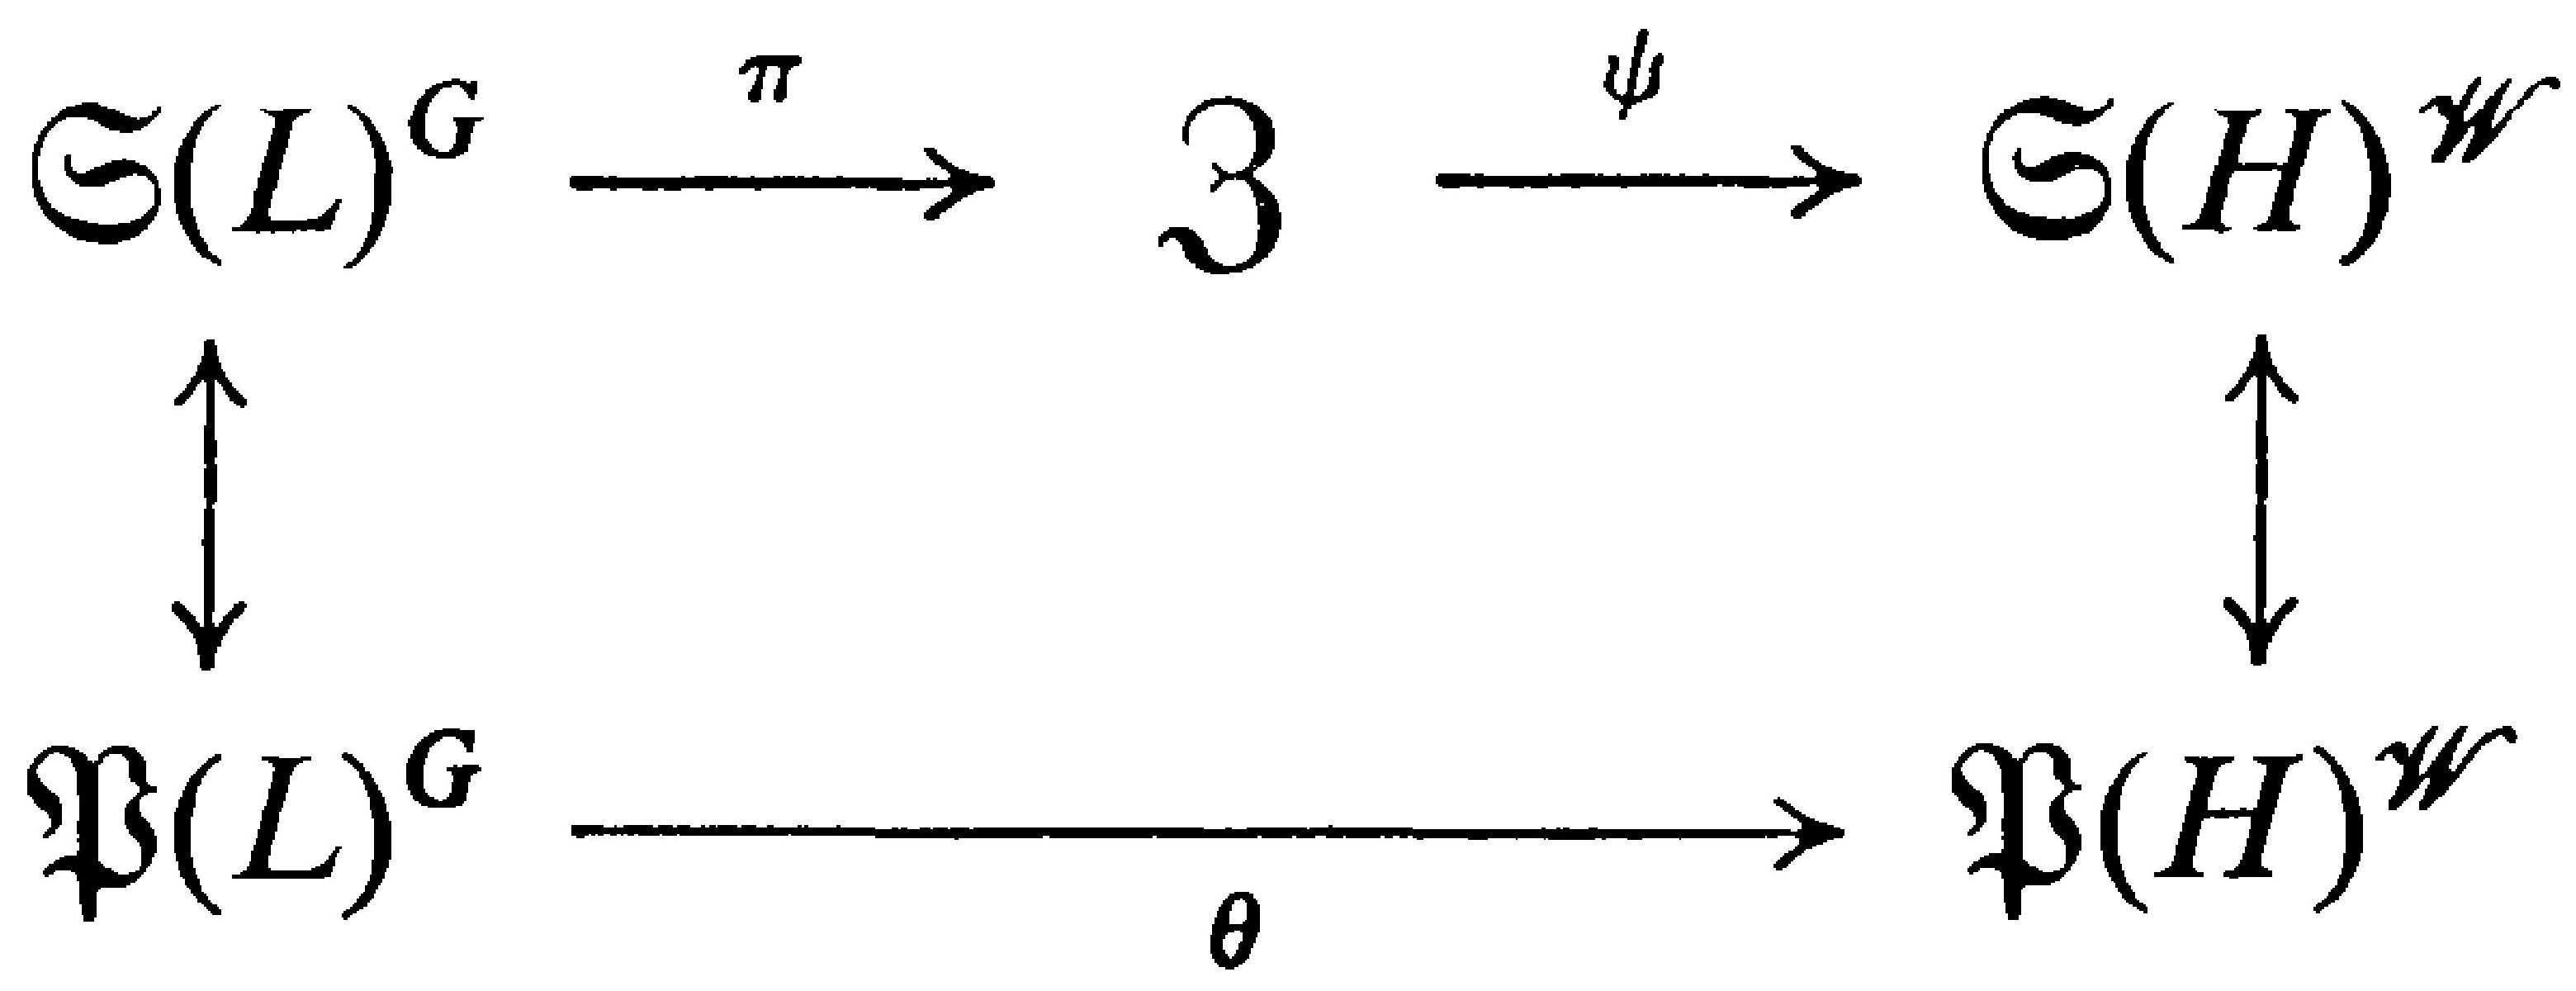
\includegraphics[max width=\textwidth, center]{2025_06_06_fac2836a92464059da43g-144}

Unfortunately, this diagram is not quite commutative. To see what is going on, we pause to look at a simple example.

Example. Let $L=\mathfrak{s l}(2, \mathrm{~F})$, with standard basis $(x, y, h)$. The dual basis ( $x^{*}, y^{*}, h^{*}$ ) may be identified with ( $\frac{1}{4} y, \frac{1}{4} x, \frac{1}{8} h$ ) via the Killing form (Exercise 5.5). If $\lambda$ is the fundamental dominant weight ( $\lambda=\frac{1}{2} \alpha$ ), then $\lambda$ identifies here with $h^{*}$, and $\lambda^{2}$ generates $\mathfrak{B}(H)^{\mathscr{W}}$. $\lambda$ being the highest weight of the usual representation of $L$, an easy calculation (Exercise 1) shows that the trace polynomial $h^{* 2}+x^{*} y^{*}$ equals $\theta^{-1}\left(\lambda^{2}\right)$. Under the identification of $\mathfrak{B}(L)^{G}$ with $\mathfrak{S}(L)^{G}$, this becomes the symmetric tensor $(1 / 64)(h \otimes h)+(1 / 32)$ $(x \otimes y+y \otimes x) . \pi$ maps this element to $(1 / 64) h^{2}+(1 / 32) x y+(1 / 32) y x \in 3$. In turn, to calculate the image under $\psi$, we must rewrite this element in the PBW basis (relative to the ordering $y, h, x)$ as $(1 / 64) h^{2}+(2 / 32) y x+(1 / 32) h$. $\xi$ sends this to $(1 / 64)\left(h^{2}+2 h\right)$, and $\eta$ in turn to the $\mathscr{W}$-invariant $(1 / 64)$ $\left(h^{2}-1\right)$. Reverting to $\mathfrak{P}(H)^{\mathscr{W}}$, this yields $\lambda^{2}-1 / 64$. Therefore, the diagram does fail to commute. Nevertheless, the discrepancy is measured by an invariant (here the scalar $1 / 64$ ) of lower "degree" than the element we started with.

This example suggests how to complete the proof that $\psi$ is surjective (for $\mathfrak{s l}(2, \mathrm{~F})$, it is the proof!). First of all, we agree to identify $\mathfrak{B}(L)^{G}$ with $\mathfrak{S}(L)^{G}$ and $\mathfrak{P}(H)^{\mathscr{W}}$ with $\mathfrak{S}(H)^{\mathscr{W}}$. Next, it is obvious that if a polynomial in $\mathfrak{G}(H)$ is fixed by $\mathscr{W}$, then so are its homogeneous parts. Therefore, it will suffice to lift homogeneous polynomials to 3 ; in particular, we can use induction on degree (constants being trivially liftable).

The maps $\theta$ and $\xi \circ \pi$ are now essentially the same (recall how each is defined), except that we have to rewrite the "symmetric" element $\pi(f)$ in the PBW basis before applying $\xi$. This introduces some new terms. However, if $f$ has degree $k$, then $\pi(f)$ is a sum of terms $x_{1} \ldots x_{k}$ in $\mathfrak{U}(L)\left(x_{i}\right.$ among the fixed basis elements of $L$ ), so the new terms obtained by commutating clearly have the form $x_{1} \ldots x_{j}$ for $j<k$.

The map $\eta$ (sending $h_{i}$ to $h_{i}-1$ ) has no effect on highest degree terms of polynomials in $\mathfrak{S}(H)$. The upshot is that we recover our original homogeneous element of $\mathfrak{S}(H)^{\mathscr{W}}$, modulo terms of lower degree, when we go around the diagram using $\theta^{-1}$, then $\pi$, then $\psi$. The lower degree terms are, by induction, images under $\psi$ of elements of 3 , so the argument is complete.

\section*{Appendix}
One fact was left unproved in this section: that the restriction map $\mathfrak{B}(L)^{G}$ $\rightarrow \mathfrak{B}(H)^{\mathscr{W}}$ is injective (23.1). This fact is inessential to the proof of HarishChandra's Theorem, but it would be less than satisfactory to pass over it in silence. It can be formulated as a simple density argument within the framework of (affine) algebraic geometry.

Let $\mathrm{A}=\mathrm{F}^{n}$ (called affine n -space); we ignore the vector space structure of A here. Let $\mathrm{F}[T]=\mathrm{F}\left[T_{1}, \ldots, T_{n}\right]$ be the polynomial ring in $n$ indeterminates.

If $I$ is an ideal in $\mathrm{F}[T]$, let $\mathscr{V}(I)=\left\{x=\left(x_{1}, \ldots, x_{n}\right) \in \mathrm{A} \mid f(x)=0\right.$ for all $f \in I\}$. We topologize A by declaring the sets $\mathscr{V}(I)$ to be closed; obviously $\varnothing$ and A are closed, while the fact that finite unions or arbitrary intersections of closed sets are closed is easy to verify (using, e.g., $\mathscr{V}\left(\sum_{\alpha} I_{\alpha}\right)=\bigcap_{\alpha} \mathscr{V}\left(I_{\alpha}\right)$ ). This topology on A is called the Zariski topology. (In case $\mathbf{F}=\mathbf{R}$ or $\mathbf{C}$, a Zariski-closed set is also closed in the usual topology on $F^{n}$, but not conversely.)

If $f(T) \in \mathrm{F}[T]$, the function $x \mapsto f(x)(\mathrm{A} \rightarrow \mathrm{F})$ is called a polynomial function on A. Evidently such a function is continuous in the Zariski topology, $F$ being given the Zariski topology of affine 1 -space. Since $F$ is infinite, the only polynomial vanishing on $A$ is the zero polynomial (as is well known).

A subset of $A$ is called irreducible if it cannot be covered by two closed sets neither of which already covers it. ("Irreducible" implies "connected", but not conversely.)

Lemma. A is irreducible.\\
Proof. Let $\mathrm{A}=\mathscr{V}\left(I_{1}\right) \cup \mathscr{V}\left(I_{2}\right)$, and suppose both of these closed sets are proper. Then $I_{1} \neq 0, I_{2} \neq 0$. Let $f \in I_{1}, g \in I_{2}$ be nonzero polynomials. Then $f g \neq 0$, but $f g$ vanishes identically on A , which is absurd.

Corollary. Any nonempty open set in A is dense.\\
Proof. Let $U$ be a nonempty open set. If $U$ is not dense, then there exists a nonempty open set $V$ in A with $U \cap V=\varnothing$; the closed sets A $-U$, A $-V$ are then proper, and cover A, contradicting the lemma.

Return now to the situation of §23: $L$ semisimple, $H$ a CSA (etc.). Fix a basis of $L$, so that $L$ becomes identified with affine $n$-space ( $n=\operatorname{dim} L$ ) and $\mathfrak{P}(L)$ with the polynomial functions in the above sense. Relative to this basis, ad $x$ is represented by an $n \times n$ matrix, whose coordinates are linear (hence polynomial) functions on $L$. In turn, let $T$ be an indeterminate, and write (for $x \in L$ ) $p_{x}(T)=$ characteristic polynomial of ad $x=\sum_{i=0}^{n} c_{i}(x) T^{i}$. It is clear that each $c_{i}$ is a polynomial function on $L$.

Call the $\rho$-rank of $L$ the smallest integer $m$ for which $c_{m}$ is not identically 0 , and call $x \in L \rho$-regular if $c_{m}(x) \neq 0$. In words, $x$ is $\rho$-regular if and only if 0 has the smallest possible multiplicity as an eigenvalue of ad $x$. This shows that $x$ is $\rho$-regular if and only if $x_{s}$ is (since they have the same characteristic polynomial); in particular, $\rho$-regular semisimple elements exist. Obviously the set $\mathscr{R}$ of all $\rho$-regular elements of $L$ is open; being open and nonempty, it is dense (by the above corollary).

If $x \in L$ is semisimple, $x$ lies in a maximal toral subalgebra, so the conjugacy theorem implies that $x$ is conjugate under $G$ to some element of $H$. But if $h \in H$, we know that $\operatorname{dim} C_{L}(h) \geq \ell=\operatorname{rank} L$; we also know that $H$ possesses elements (called regular) for which $\operatorname{dim} C_{L}(h)=\ell$ (15.3). Since $\rho$-regular semisimple elements exist, they must therefore coincide with the regular semisimple elements (and $m=\ell$ ). But no nilpotent element other\\
than 0 centralizes a regular semisimple element. In view of the preceding paragraph, $x \rho$-regular implies $x=x_{s}$. This allows us to describe $\mathscr{R}$ as the set of all regular semisimple elements.

Now let $f \in \mathfrak{B}(L)^{G},\left.f\right|_{H}=0$. This implies in particular that $f$ vanishes on $\mathscr{R}$, which is dense, so $f=0$. Therefore $\theta: \mathfrak{B}(L)^{G} \rightarrow \mathfrak{B}(H)^{\mathscr{W}}$ is injective.

\section*{Exercises}
\begin{enumerate}
  \item In the Example in (23.3), verify that the trace polynomial is given correctly.
  \item For the algebras of type $A_{2}, B_{2}, G_{2}$, compute explicit generators for $\mathfrak{B}(H)^{\mathscr{W}}$ in terms of the fundamental dominant weights $\lambda_{1}, \lambda_{2}$. Show how some of these lift to $\mathcal{O}$, using the algorithm of this section. (Notice too that in each case $\mathfrak{B}(H)^{\mathscr{W}}$ is a polynomial algebra with $\ell=2$ generators.)
  \item Show that Proposition 23.2 remains valid when $\lambda$ is an arbitrary linear function on $H$, provided only that $\langle\lambda, \alpha\rangle$ is an integer.
  \item From the formula $\left({ }^{*}\right) \chi_{\lambda}(z)=\lambda(\xi(z))$ of (23.3), compute directly the value of the universal Casimir element $c_{L}$ (22.1) on $V(\lambda), \lambda \in \Lambda^{+}:(\lambda+\delta, \lambda+\delta)-$ $(\delta, \delta)$. [Recall how $t_{\alpha}$ and $h_{\alpha}$, resp. $z_{\alpha}$ and $y_{\alpha}$, are related. Rewrite $c_{L}$ in the ordering of a PBW basis, and use the fact derived in (22.3) that $(\mu, \mu)=$ $\sum_{i} \mu\left(h_{i}\right) \mu\left(k_{i}\right)$ for any weight $\mu$.]
  \item Prove that any polynomial in $n$ variables over $F$ (char $F=0$ ) is a linear combination of powers of linear polynomials. [Use induction on $n$. Expand $\left(T_{1}+a T_{2}\right)^{k}$ and then use a Vandermonde determinant argument to show that $k$ th powers of linear polynomials span a space of correct dimension when $n=2$.]
  \item If $\lambda \in \Lambda^{+}$prove that all $\mu$ linked to $\lambda$ satisfy $\mu \prec \lambda$, hence that all such $\mu$ occur as weights of $Z(\lambda)$.
  \item Let $\mathfrak{D}=[\mathfrak{U}(L), \mathfrak{U}(L)]$ be the subspace of $\mathfrak{U}(L)$ spanned by all $x y-y x$ $(x, y \in \mathfrak{U}(L))$. Prove that $\mathfrak{U}(L)$ is the direct sum of the subspaces $\mathfrak{D}$ and 3 (thereby allowing one to extend $\chi_{\lambda}$ to all of $\mathfrak{U}(L)$ by requiring it to be 0 on $\mathfrak{D}$ ). [Recall from Exercise 17.3 that $\mathfrak{U}(L)$ is the sum of finite dimensional $L$-modules, hence is completely reducible because $L$ is semisimple. Show that 3 is the sum of all trivial $L$-submodules of $\mathfrak{U}(L)$, while $\mathfrak{D}$ coincides with the space of all ad $x(y), x \in L, y \in \mathfrak{U}(L)$, the latter being complementary to 3.]
  \item Prove that the weight lattice $\Lambda$ is Zariski dense in $H^{*}$ (see Appendix), $H^{*}$ being identified with affine $\ell$-space. Use this to give another proof that Corollary' in (23.2) extends to all $\lambda, \mu \in H^{*}$.
  \item Every F-algebra homomorphism $\chi: 3 \rightarrow \mathrm{~F}$ is of the form $\chi_{\lambda}$ for some $\lambda \in H^{*}$. [View $\chi$ as a homomorphism $\mathfrak{S}(H)^{\mathscr{W}} \rightarrow \mathrm{F}$ and show that its kernel generates a proper ideal in $\mathfrak{S}(H)$.]
  \item Prove that the map $\psi: 3 \rightarrow \mathbb{S}(H)^{\mathscr{W}}$ is independent of the choice of $\Delta$.
\end{enumerate}

\section*{Notes}
Steinberg's proof of Chevalley's theorem 23.1 is written down in Verma [1], and in Varadarajan [1]. For accounts of Harish-Chandra's work on "characters", see Bourbaki [3], Harish-Chandra [1], Séminaire "Sophus Lie" [1], Exposé 19, Varadarajan [1], Verma [1]. Chevalley [5] shows that $\mathbb{S}(H)^{\mathscr{W}}$ is a polynomial algebra.

\section*{24. Formulas of Weyl, Kostant, and Steinberg}
The notation is that of §23. We are going to use Harish-Chandra's Theorem (23.3) to obtain several remarkable formulas for the characters and multiplicities of finite dimensional $L$-modules. (For a shortcut, avoiding the use of §23, see the Appendix below.)

\subsection*{24.1. Some functions on $H^{*}$}
For $\lambda \in \Lambda^{+}$, the formal character $c h_{\lambda}$ of $V(\lambda)$ was introduced in (22.5): $c h_{\lambda}=\sum_{\mu \in \Lambda} m_{\lambda}(\mu) e(\mu)$, where the $e(\mu)$ form a basis for the group ring $\mathbf{Z}[\Lambda]$. It is also convenient to define formal characters for the infinite dimensional modules $Z(\lambda)$, but here the infinite formal sums would be awkward to manipulate. Instead, we use a more suggestive formalism. $\mathbf{Z}[\Lambda]$ can be viewed as the set of $\mathbf{Z}$-valued functions on $\Lambda$ ( 0 outside a finite set); the reader can easily check that the product operation becomes convolution, $f * g(\lambda)=\sum_{\mu+\nu=\lambda} f(\mu) g(\nu)$.

Let $\mathfrak{X}$ be the space of all F -valued functions $f$ on $H^{*}$ whose support (defined to be the set of $\lambda \in H^{*}$ for which $f(\lambda) \neq 0$ ) is included in a finite union of sets of the form $\left\{\lambda-\sum_{\alpha>0} k_{\alpha}, k_{\alpha} \in \mathbf{Z}^{+}\right\}$. (Such a set is of course the set of weights occurring in a module $Z(\lambda), \lambda \in H^{*}$.)

A moment's thought shows that $\mathfrak{X}$ is closed under convolution; thus it becomes a commutative, associative $F$-algebra, containing the formal character $c h_{V}$ of any standard cyclic $L$-module.

The reader may find it convenient at times to think of $f \in \mathfrak{X}$ as a formal combination (with F-coefficients) of the $\lambda \in H^{*}$. What corresponds to our earlier $e(\lambda)$ ? Clearly this is just the characteristic function $\varepsilon_{\lambda}(\lambda)=1, \varepsilon_{\lambda}(\mu)=0$ if $\mu \neq \lambda$. Notice that $\varepsilon_{0}$ is the identity element of the ring $\mathfrak{X}$, and that $\varepsilon_{\lambda} * \varepsilon_{\mu}$ $=\varepsilon_{\lambda+\mu}$. The Weyl group $\mathscr{W}$ acts on $\mathbf{Z}[\Lambda]$ by $\left(\sigma^{-1} f\right)(\lambda)=f(\sigma \lambda)$; in particular, $\sigma\left(\varepsilon_{\lambda}\right)=\varepsilon_{\sigma \lambda}$.

Two other useful elements of $\mathfrak{X}$ must now be introduced. First, let $p(\lambda)$ be the number of sets of nonnegative integers $\left\{k_{\alpha}, \alpha \succ 0\right\}$ for which $-\lambda=\sum_{\alpha>0}$ $k_{\alpha} \alpha$. Of course, $p(\lambda)=0$ unless $\lambda$ lies in the root lattice. Notice that $p=c h_{Z(0)}$\\
(Exercise 20.5); in particular, $p \in \mathfrak{X}$. We call $p$ the Kostant function (it differs from Kostant's partition function only by a change in the sign of $\lambda$ ). Next, we let $q=\prod_{\alpha>0}\left(\varepsilon_{\alpha / 2}-\varepsilon_{-\alpha / 2}\right)$ (where the product symbol $\prod$ always denotes convolution in $\mathfrak{X}$ ). Call $q$ the Weyl function.

We shall now prove a number of simple lemmas relating the various functions defined above. Let $f_{\alpha}(-k \alpha)=1, f_{\alpha}(\lambda)=0$ otherwise, for each positive root $\alpha, k \in \mathbf{Z}^{+}$. ( $f_{\alpha}$ may be thought of symbolically as $\varepsilon_{0}+\varepsilon_{-\alpha}+\varepsilon_{-2 \alpha}$ $+\ldots)$. It is clear that $f_{\alpha} \in \mathfrak{X}$.

Lemma A. (a) $p=\prod_{\alpha>0} f_{\alpha}$.\\
(b) $\left(\varepsilon_{0}-\varepsilon_{-\alpha}\right) * f_{\alpha}=\varepsilon_{0}$.\\
(c) $q=\varepsilon_{\delta} * \prod_{\alpha \succ 0}\left(\varepsilon_{0}-\varepsilon_{-\alpha}\right)$.

Proof. (a) This follows at once from the definition of convolution. (b) Formally, $\left(\varepsilon_{0}-\varepsilon_{-\alpha}\right) *\left(\varepsilon_{0}+\varepsilon_{-\alpha}+\varepsilon_{-2 \alpha}+\ldots\right)=\varepsilon_{0}$, since all other terms cancel. (It is easy to make this rigorous.) (c) Since $\delta=\sum_{\alpha>0} \frac{1}{2} \alpha, \varepsilon_{\delta}=\prod_{\alpha>0} \varepsilon_{\alpha / 2}$. But $\left(\varepsilon_{0}-\varepsilon_{-\alpha}\right) * \varepsilon_{\alpha / 2}=\varepsilon_{\alpha^{\prime} 2}-\varepsilon_{-\alpha / 2}$, so the result follows. $\square$

Lemma B. $\sigma q=(-1)^{\ell(\sigma)} q(\sigma \in \mathscr{W}), \ell(\sigma)$ as in (10.3).\\
Proof. It suffices to prove this when $\sigma=\sigma_{\alpha}$ is a simple reflection, i.e., $\ell(\sigma)=1$. But $\sigma_{\alpha}$ permutes the positive roots other than $\alpha$ and sends $\alpha$ to $-\alpha$ (Lemma 10.2B), so $\sigma_{\alpha} q=-q$.

Lemma C. $q * p * \varepsilon_{-\delta}=\varepsilon_{0}$.\\
Proof. Combining the three parts of Lemma A, we get $q * p * \varepsilon_{-\delta}=\prod_{\alpha>0}$ $\left(\varepsilon_{0}-\varepsilon_{-\alpha}\right) * \varepsilon_{\delta} * p * \varepsilon_{-\delta}=\prod_{\alpha \succ 0}\left(\varepsilon_{0}-\varepsilon_{-\alpha}\right) * p=\prod_{\alpha>0}\left(\left(\varepsilon_{0}-\varepsilon_{-\alpha}\right) * f_{\alpha}\right)=\varepsilon_{0}$.

Lemma D. $c h_{Z(\lambda)}(\mu)=p(\mu-\lambda)=\left(p * \varepsilon_{\lambda}\right)(\mu)$.\\
Proof. The first equality is clear (cf. Exercise 20.5), the second is equally so. $\square$

Lemma E. $q * c h_{Z(\lambda)}=\varepsilon_{\lambda+\delta}$.\\
Proof. Combine Lemmas C and D. $\square$\\
The coefficient $(-1)^{\ell(\sigma)}(\sigma \in \mathscr{W})$ which appears in Lemma B will be abbreviated henceforth to $\operatorname{sn}(\sigma)$. Recall that when $L$ is of type $\mathrm{A}_{\ell}, \mathscr{W}$ is isomorphic to the symmetric group $\mathscr{S}_{\ell+1}$, and $\operatorname{sn}(\sigma)$ coincides with the sign ( + for even, - for odd) of the permutation $\sigma$.

\subsection*{24.2. Kostant's multiplicity formula}
The idea now is to express the formal character $c h_{\lambda}$ of the finite dimensional module $V(\lambda)\left(\lambda \in \Lambda^{+}\right)$as Z-linear combination of certain $c h_{Z(\mu)}$, and\\
then use the lemmas of the preceding subsection (along with HarishChandra's Theorem) to simplify the result.

Let $\mathfrak{M}_{\lambda}$ denote the collection of all $L$-modules $V$ having the following properties (for fixed $\lambda \in H^{*}$ ):\\
(1) $V$ is the direct sum of weight spaces (relative to $H$ ).\\
(2) The action of 3 on $V$ is by scalars $\chi_{\lambda}(z)(z \in \mathfrak{Z})$, for the given $\lambda \in H^{*}$. ( $3=$ center of $\mathfrak{U}(L)$.)\\
(3) The formal character of $V$ belongs to $\mathfrak{X}$. Of course, all standard cyclic modules of weight $\lambda$ meet these criteria; so do their submodules (which are known to be not always sums of standard cyclic submodules). Indeed, $\mathfrak{M}_{\lambda}$ is closed under the operations of taking submodules, taking homomorphic images, and forming (finite) direct sums. In view of Harish-Chandra's Theorem (23.3), $\mathfrak{M}_{\lambda}=\mathfrak{M}_{\mu}$ precisely when $\lambda$ and $\mu$ are linked.

Lemma. Let $V \in \mathfrak{M}_{\lambda}$. Then $V$ possesses at least one maximal vector (if $V \neq 0$ ).

Proof. Because of property (3), for each $\alpha>0$, and each weight $\mu$ of $V$, $\mu+k \alpha$ is not a weight of $V$ for all sufficiently large $k \in \mathbf{Z}^{+}$. This makes it clear that for some weight $\mu$, no $\mu+\alpha$ is a weight ( $\alpha>0$ ); any nonzero vector in $V_{\mu}$ is then maximal. $\square$

For each $\lambda \in H^{*}$, let $\theta(\lambda)=\left\{\mu \in H^{*} \mid \mu \prec \lambda\right.$ and $\left.\mu \sim \lambda\right\}$. Recall (23.2) that $\mu \sim \lambda$ means $\mu+\delta$ and $\lambda+\delta$ are $\mathscr{W}$-conjugate. In the following key result, Harish-Chandra's Theorem comes into play by limiting the possible highest weights of composition factors of $Z(\lambda)$.

Proposition. Let $\lambda \in H^{*}$. Then:\\
(a) $Z(\lambda)$ possesses a composition series.\\
(b) Each composition factor of $Z(\lambda)$ is of the form $V(\mu)$, where $\mu \in \theta(\lambda)$ and $V(\mu)$ is as defined in (20.3).\\
(c) $V(\lambda)$ occurs only once as a composition factor of $Z(\lambda)$.

Proof. (a) If $Z(\lambda)$ is irreducible, then $Z(\lambda)=V(\lambda)$, and there is nothing to prove. Otherwise $Z(\lambda)$ has a nonzero proper submodule $V$, which lies in $\mathfrak{M}_{\lambda}$ (the given $\lambda$ being used for condition (2)). Since $\operatorname{dim} Z(\lambda)_{\lambda}=1, \lambda$ does not occur as a weight of $V$. By the above lemma, $V$ has a maximal vector (say of weight $\mu \not{ }_{\neq} \lambda$ ), hence $V$ contains a nonzero homomorphic image $W$ of $Z(\mu)$. In particular, $\chi_{\lambda}=\chi_{\mu}$, so $\lambda \sim \mu$ (by Harish-Chandra's Theorem), and $\mu \in \theta(\lambda)$. Consider now $Z(\lambda) / W, W$. Each module is standard cyclic (and lies in $\mathfrak{M}_{\lambda}$ ), but either has fewer weights linked to $\lambda$ than $Z(\lambda)$ had, or else has the same weights linked to $\lambda$, but some of smaller multiplicity than in $Z(\lambda)$. Repetition of the above argument for $Z(\lambda) / W$ and $W$ leads to further submodules and homomorphic images of submodules, with decreasing number of weights linked to $\lambda$ or else decreasing multiplicities for those weights. This makes it evident that the process will end after finitely many steps, with a composition series for $Z(\lambda)$.\\
(b) Each composition factor of $Z(\lambda)$ lies in $\mathfrak{M}_{\lambda}$, hence possesses a maximal vector (by the lemma), hence must be standard cyclic (being irreducible). In\\
view of (20.2), each composition factor is isomorphic to some $V(\mu)$. We saw already that $\mu$ must then belong to $\theta(\lambda)$.\\
(c) This is clear, since $\operatorname{dim} Z(\lambda)_{\lambda}=1$.

The proposition allows us to write $c h_{Z(\lambda)}=c h_{V(\lambda)}+\sum d(\mu) c h_{V(\mu)}(d(\mu) \in$ $\mathbf{Z}^{+}$), where the summation is taken over $\mu \in \theta(\lambda), \mu \neq \lambda$. With $\lambda \in H^{*}$ still fixed, order the elements of $\theta(\lambda)$ as ( $\mu_{1}, \ldots, \mu_{t}$ ), subject only to the condition that $\mu_{i} \prec \mu_{j}$ imply $i \leq j$. (In particular, $\lambda=\mu_{t}$.) According to the proposition, each $c h_{Z\left(\mu_{j}\right)}$ may in turn be expressed as a Z-linear combination of the $c h_{V\left(\mu_{i}\right)}$ with $i \leq j$ ( $c h_{V\left(\mu_{j}\right)}$ occurring with coefficient one). Therefore the resulting system of $t$ equations has triangular matrix, relative to the chosen order, with ones on the diagonal; in particular, its determinant is 1 , so we can invert it over $\mathbf{Z}$ and express each $c h_{V\left(\mu_{j}\right)}$ as $\mathbf{Z}$-linear combination of the $c h_{Z\left(\mu_{i}\right)}$ for $i \leq j, c h_{Z\left(\mu_{j}\right)}$ occurring with coefficient one. (Of course, some coefficients may now be negative.)

Corollary. Let $\lambda \in H^{*}$. Then $c h_{V(\lambda)}$ is a Z-linear combination $\sum c(\mu) c h_{Z(\mu)}$ (summation over $\mu \in \theta(\lambda)$ ), with $c(\lambda)=1$.

We now apply the corollary to the special case in which $\lambda$ is dominant integral, $c h_{\lambda}=c h_{V(\lambda)}$. Then $\operatorname{dim} V(\lambda)$ is finite, and $\sigma\left(c h_{\lambda}\right)=c h_{\lambda}$ for all $\sigma \in \mathscr{W}$ (Theorem 21.2). Write $c h_{\lambda}=\sum c(\mu) c h_{Z(\mu)}(\mu \in \theta(\lambda))$ as above, with $c(\lambda)=1$. By Lemma E of (24.1), $q * c h_{\lambda}=\sum c(\mu) \varepsilon_{\mu+\delta}$. By Lemma B of (24.1), $\sigma\left(q * c h_{\lambda}\right)$ $=\sigma(q) * \sigma\left(c h_{\lambda}\right)=\operatorname{sn}(\sigma) q * c h_{\lambda}(\sigma \in \mathscr{W})$. On the other hand, $\sigma\left(\sum c(\mu) \varepsilon_{\mu+\delta}\right)=$ $\sum c(\mu) \varepsilon_{\sigma(\mu+\delta)}$. Since $\mathscr{W}$ just permutes the $\mu+\delta$ transitively ( $\mu$ being linked to $\lambda$ ), while $c(\lambda)=1$, it follows immediately that $c(\mu)=\operatorname{sn}(\sigma)$ if $\sigma^{-1}(\mu+\delta)=$ $\lambda+\delta$. Therefore


\begin{equation*}
q * c h_{\lambda}=\sum_{\sigma \in \mathscr{W}} \operatorname{sn}(\sigma) \varepsilon_{\sigma(\lambda+\delta)} \tag{*}
\end{equation*}


Finally, apply Lemma C of (24.1) to this equation to obtain: $c h_{\lambda}=q * p *$ $\varepsilon_{-\delta} * c h_{\lambda}=p * \varepsilon_{-\delta} *\left(\sum_{\sigma \in \mathscr{W}} \operatorname{sn}(\sigma) \varepsilon_{\sigma(\lambda+\delta)}\right)=p *\left(\sum_{\sigma \in \mathscr{W}} \operatorname{sn}(\sigma) \varepsilon_{\sigma(\lambda+\delta)-\delta}\right)=\sum_{\sigma \in \mathscr{W}} \operatorname{sn}(\sigma)$ $p * \varepsilon_{\sigma(\lambda+\delta)-\delta}$.

Theorem (Kostant). Let $\lambda \in \Lambda^{+}$. Then the multiplicities of $V(\lambda)$ are given by the formula

$$
m_{\lambda}(\mu)=\sum_{\sigma \in \mathscr{W}} \operatorname{sn}(\sigma) p(\mu+\delta-\sigma(\lambda+\delta)) .
$$

This formula has the virtue of expressing multiplicities directly. However, Freudenthal's recursive method (§22) is often simpler to use in practice, because summation over the Weyl group becomes very cumbersome in high rank.

\subsection*{24.3. Weyl's formulas}
Lemma. $q=\sum_{\sigma \in \mathscr{W}} \operatorname{sn}(\sigma) \varepsilon_{\sigma \delta}$.\\
Proof. This is easy to prove directly, but instead we use formula (*) of (24.2). If $\lambda=0$, then of course $c h_{\lambda}=\varepsilon_{0}$, and the right side of $(*)$ becomes $\sum_{\sigma \in \mathscr{W}}$ $\operatorname{sn}(\sigma) \varepsilon_{\sigma \delta} . \quad \square$

Theorem (Weyl). Let $\lambda \in \Lambda^{+}$. Then $\left(\sum_{\sigma \in \mathscr{W}} \operatorname{sn}(\sigma) \varepsilon_{\sigma \delta}\right) * \operatorname{ch}{ }_{\lambda}=\sum_{\sigma \in \mathscr{W}} \operatorname{sn}(\sigma) \varepsilon_{\sigma(\lambda+\delta)}$.\\
Proof. Use formula (*) in (24.2) along with the above lemma. $\square$\\
Weyl's character formula says in effect that we may calculate $c h_{\lambda}$ as a quotient of two simple alternating sums in $\mathbf{Z}[\Lambda]$. In practice the carrying out of this "division" can be quite laborious, so Freudenthal's method (§22) is usually quicker. However, we can derive from Weyl's formula an extremely useful formula for the dimension of $V(\lambda)\left(\lambda \in \Lambda^{+}\right)$, which we denote by $\operatorname{deg}(\boldsymbol{\lambda})$. It is clear that $\operatorname{deg}(\lambda)=\sum_{\mu \in \Pi(\lambda)} m_{\lambda}(\mu)$, since $V(\lambda)$ is direct sum of weight spaces. This is just the sum of coefficients in the formal sum $\sum_{\mu} m_{\dot{\lambda}}(\mu)$ $e(\mu) \in \mathbf{Z}[\Lambda]$. In the function notation, this becomes the sum of the values of $c h_{\lambda}$. Let us work now in the subalgebra $\mathfrak{X}_{0} \subset \mathfrak{X}$ generated by the characteristic functions $\varepsilon_{\lambda}(\lambda \in \Lambda)$, so the homomorphism $v: \mathfrak{X}_{0} \rightarrow \mathrm{~F}$ assigning to $f \in \mathfrak{X}_{0}$ the sum of its values is defined. Our problem is to compute $v\left(c h_{\lambda}\right)$ as a function of $\lambda$. Unfortunately, applying $v$ to an alternating sum such as $\sum \operatorname{sn}(\sigma) \varepsilon_{\sigma \delta}$ gives 0 , so we must proceed indirectly. Abbreviate $\sum \operatorname{sn}(\sigma) \varepsilon_{\sigma(\lambda+\delta)}$ by $\omega(\lambda+\delta)$, for any $\lambda \in \Lambda^{+}$.

The assignment $\varepsilon_{\lambda} \mapsto(\lambda, \alpha) \varepsilon_{\lambda}$ (for fixed root $\alpha$ ) extends to an endomorphism $\partial_{\alpha}$ of $\mathfrak{X}_{0}$, which is in fact a derivation. The endomorphism $\partial=\prod_{\alpha \succ 0} \partial_{\alpha}$ is no longer a derivation, in general, but may be thought of as a differential operator. Weyl's formula reads: $\omega(\delta) * c h_{\lambda}=\omega(\lambda+\delta)$. Here $\omega(\delta)$ is the Weyl function (denoted $q$ earlier), which equals $\varepsilon_{-\delta^{*}} \prod_{\alpha>0}\left(\varepsilon_{\alpha}-1\right)$ (cf. Lemma 24.1A(c)). Multiply this expression by $c h_{\lambda}$ and apply $\partial$ (using the product rule for the derivations $\partial_{\alpha}$ ), then $v$. Most of the resulting terms vanish, since $v\left(\varepsilon_{\alpha}-1\right)=0$. What survives is $v(\partial \omega(\delta)) v\left(c h_{\lambda}\right)$, which by Weyl's formula must equal $v(\partial \omega(\lambda+\delta))$. This allows us to express $\operatorname{deg}(\lambda)=$ $v\left(c h_{\lambda}\right)$ as a quotient.

A moment's thought shows that $v\left(\partial \varepsilon_{\delta}\right)=\prod_{\alpha \succ 0}(\delta, \alpha)$; similarly, $v\left(\partial \varepsilon_{\sigma \delta}\right)=\prod_{\alpha \succ 0}$ $(\sigma \delta, \alpha)=\prod_{\alpha>0}\left(\delta, \sigma^{-1} \alpha\right)$. But recall that the number of positive roots sent to negative roots by $\sigma^{-1}$ is $\ell\left(\sigma^{-1}\right)=\ell(\sigma)$ (cf. Lemma A (10.3)), so this is just $\operatorname{sn}(\sigma) \prod_{\alpha>0}(\delta, \alpha), \operatorname{sn}(\sigma)=(-1)^{\ell(\sigma)}$. In other words, $v(\partial \omega(\delta))=\sum_{\sigma \in \mathscr{W}} \operatorname{sn}(\sigma) v\left(\partial \varepsilon_{\sigma \delta}\right)$ $=\sum_{\sigma \in \mathscr{W}}^{\alpha>0} \operatorname{sn}(\sigma)^{2} \prod_{\alpha \succ 0}(\delta, \alpha)=\operatorname{Card}(\mathscr{W}) \prod_{\alpha \succ 0}(\delta, \alpha)$. The same argument for $\omega(\lambda+\delta)$ leads to Card $\mathscr{W}) \prod_{\alpha>0}(\lambda+\delta, \alpha)$. Forming the quotient we therefore have:

Corollary. Let $\lambda \in \Lambda^{+}$. Then $\operatorname{deg}(\lambda)=\frac{\prod_{\alpha>0}(\lambda+\delta, \alpha)}{\prod_{\alpha>0}(\delta, \alpha)} . \quad \square$\\
In order to compute some examples, we observe that after multiplying both numerator and denominator by $\prod_{\alpha>0} \frac{2}{(\alpha, \alpha)}$, we get $\operatorname{deg}(\lambda)=\frac{\prod_{\alpha \succ 0}\langle\lambda+\delta, \alpha\rangle}{\prod_{\alpha \succ 0}\langle\delta, \alpha\rangle}$ (a quotient of integers). But $<\lambda+\delta, \alpha>=\left(\lambda+\delta, \alpha^{\nu}\right), \alpha^{\nu}$ the dual root. In\\
turn, since $\Delta^{\vee}$ is a base of $\Phi^{\vee}$ (Exercise 10.1), we can write $\alpha^{\vee}=\sum_{i} c_{i}{ }^{(\alpha)} \alpha_{i}{ }^{\vee}$, whence $\langle\lambda+\delta, \alpha\rangle=\sum_{i} c_{i}{ }^{(\alpha)}<\lambda+\delta, \alpha_{i}>=\sum_{i} c_{i}{ }^{(\alpha)}\left(m_{i}+1\right)\left(\lambda=\sum_{i} m_{i} \lambda_{i}\right)$. So we need only compute the integers $c_{i}{ }^{(\alpha)}$ (Exercise 7).

Examples. For type $A_{1}, \lambda_{1}=\frac{1}{2} \alpha=\delta$, so the formula reads: $\operatorname{deg}(\lambda)=$ $m+1, \lambda=m \lambda_{1}$, cf. Theorem 7.2.

Let us concentrate now on rank 2 , writing $\lambda=m_{1} \lambda_{1}+m_{2} \lambda_{2}$. For type $\mathrm{A}_{2}$ the positive roots are $\alpha_{1}, \alpha_{2}, \alpha_{1}+\alpha_{2}$. Accordingly, the denominator above equals $1 \cdot 1 \cdot 2$, while the numerator is $\left(m_{1}+1\right)\left(m_{2}+1\right)\left(m_{1}+m_{2}+2\right)$. For $\mathrm{B}_{2}$ and $G_{2}$ the calculations are similar (take $\alpha_{2}$ short for $B_{2}, \alpha_{1}$ short for $G_{2}$, in conformity with §11). To summarize (Exercise 7):\\
( $\left.\mathrm{A}_{2}\right) \frac{1}{2}\left(m_{1}+1\right)\left(m_{2}+1\right)\left(m_{1}+m_{2}+2\right)$\\
( $\left.\mathrm{B}_{2}\right) \frac{1}{3!}\left(m_{1}+1\right)\left(m_{2}+1\right)\left(m_{1}+m_{2}+2\right)\left(2 m_{1}+m_{2}+3\right)$\\
$\left(\mathrm{G}_{2}\right) \frac{1}{5!}\left(m_{1}+1\right)\left(m_{2}+1\right)\left(m_{1}+m_{2}+2\right)\left(m_{1}+2 m_{2}+3\right)\left(m_{1}+3 m_{2}+4\right)\left(2 m_{1}+\right.$ $\left.3 m_{2}+5\right)$.\\
For $G_{2}, \operatorname{deg}\left(\lambda_{2}\right)=14$. Since $\lambda_{2}=3 \alpha_{1}+2 \alpha_{2}$, the highest root, we recognize $V\left(\lambda_{2}\right)$ as the module for the adjoint representation. Deg $\left(\lambda_{1}\right)=7$. Here $V\left(\lambda_{1}\right)$ is $\mathscr{C}_{o}$ (the trace 0 subspace of the Cayley algebra (19.3)).

\subsection*{24.4. Steinberg's formula}
We can combine the formulas of Kostant and Weyl to obtain an explicit formula (due to R. Steinberg) for the number of occurrences of $V(\lambda)$ in the tensor product $V\left(\lambda^{\prime}\right) \otimes V\left(\lambda^{\prime \prime}\right)$. Because of Weyl's Theorem on complete reducibility of finite dimensional $L$-modules (6.3), if $\lambda^{\prime}, \lambda^{\prime \prime} \in \Lambda^{+}$, we can write $V\left(\lambda^{\prime}\right) \otimes V\left(\lambda^{\prime \prime}\right)$ as direct sum of certain $V(\lambda)$, each occurring $n(\lambda)$ times (write $n(\lambda)=0$ if $V(\lambda)$ does not occur at all). In particular, the formal character of the tensor product equals $\sum_{\lambda \in \Lambda^{+}} n(\lambda) c h_{\lambda}$. On the other hand, we proved in (22.5) that this formal character equals $c h_{\lambda^{\prime}} * c h_{\lambda^{\prime \prime}}$. Thus:


\begin{equation*}
c h_{\lambda^{\prime}} * c h_{\lambda^{\prime \prime}}=\sum_{\lambda} n(\lambda) c h_{\lambda} . \tag{1}
\end{equation*}


As before, let us abbreviate the expression $\sum_{\sigma \in \mathscr{W}} \operatorname{sn}(\sigma) \varepsilon_{\sigma(\mu+\delta)}$ to $\omega(\mu+\delta)$, for $\mu \in \Lambda^{+}$. If we multiply both sides of (1) by $\omega(\delta)$ and use Weyl's formula (24.3) for $\lambda^{\prime \prime}, \lambda$ (respectively), we get:


\begin{equation*}
c h_{\lambda^{\prime}} * \omega\left(\lambda^{\prime \prime}+\delta\right)=\sum_{\lambda} n(\lambda) \omega(\lambda+\delta) . \tag{2}
\end{equation*}


Next we write $c h_{\lambda^{\prime}}=\sum_{\mu} m_{\lambda^{\prime}}(\mu) \varepsilon_{\mu}$ and replace $m_{\lambda^{\prime}}(\mu)$ by its value in Kostant's formula (24.2). Equation (2) then becomes:


\begin{equation*}
\sum_{\mu} \sum_{\sigma \in \mathscr{W}} \operatorname{sn}(\sigma) p\left(\mu+\delta-\sigma\left(\lambda^{\prime}+\delta\right)\right) \varepsilon_{\mu} * \omega\left(\lambda^{\prime \prime}+\delta\right)=\sum_{\lambda} n(\lambda) \omega(\lambda+\delta) . \tag{3}
\end{equation*}


Using the explicit form of $\omega\left(\lambda^{\prime \prime}+\delta\right)$, this reads:


\begin{align*}
\sum_{\mu} \sum_{\sigma \in \mathscr{W}} \sum_{\tau \in \mathscr{W}} \operatorname{sn}(\sigma \tau) p\left(\mu+\delta-\sigma\left(\lambda^{\prime}+\delta\right)\right) \varepsilon_{\tau\left(\lambda^{\prime \prime}+\delta\right)+\mu} &  \tag{4}\\
& =\sum_{\lambda} \sum_{\sigma \in \mathscr{W}} n(\lambda) \operatorname{sn}(\sigma) \varepsilon_{\sigma(\lambda+\delta)} .
\end{align*}


To compare the two sides of (4) we first change variables. On the right, replace $\lambda$ by $\nu$, where $\sigma(\lambda+\delta)=\nu+\delta$, to get


\begin{equation*}
\sum_{\nu} \sum_{\sigma \in \mathscr{W}} \operatorname{sn}(\sigma) n(\sigma(\nu+\delta)-\delta) \varepsilon_{\nu+\delta} . \tag{5}
\end{equation*}


On the left, replace $\mu$ by $\nu$, where $\tau\left(\lambda^{\prime \prime}+\delta\right)+\mu=\nu+\delta$, obtaining:


\begin{equation*}
\sum_{\nu} \sum_{\sigma \in \mathscr{W}} \sum_{\tau \in \mathscr{W}} \operatorname{sn}(\sigma \tau) p\left(\nu+2 \delta-\sigma\left(\lambda^{\prime}+\delta\right)-\tau\left(\lambda^{\prime \prime}+\delta\right)\right) \varepsilon_{\nu+\delta} . \tag{6}
\end{equation*}


Now let $\nu$ be dominant. Then $\sigma(\nu+\delta)-\delta$ cannot be dominant unless $\sigma=1$ (Exercise 13.10). Therefore, $n(\sigma(\nu+\delta)-\delta)=0$ unless $\sigma=1$, which means that the coefficient of $\varepsilon_{v+\delta}$ in (5) is precisely $n(\nu)$. In view of (6), we have proved:

Theorem (Steinberg). Let $\lambda^{\prime}, \lambda^{\prime \prime} \in \Lambda^{+}$. Then the number of times $V(\lambda)$, $\lambda \in \Lambda^{+}$, occurs in $V\left(\lambda^{\prime}\right) \otimes V\left(\lambda^{\prime \prime}\right)$ is given by the formula

$$
\sum_{\sigma \in \mathscr{W}} \sum_{\tau \in \mathscr{W}} \operatorname{sn}(\sigma \tau) p\left(\lambda+2 \delta-\sigma\left(\lambda^{\prime}+\delta\right)-\tau\left(\lambda^{\prime \prime}+\delta\right)\right) .
$$

This formula (like Kostant's) is very explicit, but not at all easy to apply when the Weyl group is large. A formula which is often more practical is developed in Exercise 9.

\section*{Exercises}
\begin{enumerate}
  \item Give a direct proof of Weyl's character formula (24.3) for type $A_{1}$.
  \item Use Weyl's dimension formula to show that a faithful irreducible finite dimensional $L$-module of smallest possible dimension has highest weight $\lambda_{i}$ for some $1 \leq i \leq \ell$.
  \item Use Kostant's formula to check some of the multiplicities listed in Example 1 (22.4), and compare $c h_{\lambda}$ there with the expression given by Weyl's formula.
  \item Compare Steinberg's formula for the special case $\mathrm{A}_{1}$ with the ClebschGordan formula (Exercise 22.7).
  \item Using Steinberg's formula, decompose the $\mathrm{G}_{2}$-module $V\left(\lambda_{1}\right) \otimes V\left(\lambda_{2}\right)$ into its irreducible constituents. Check that the dimensions add up correctly to the product $\operatorname{dim} V\left(\lambda_{1}\right) \cdot \operatorname{dim} V\left(\lambda_{2}\right)$, using Weyl's formula.
  \item Let $L=\mathfrak{s l}(3, \mathfrak{F})$. Abbreviate $\lambda=m_{1} \lambda_{1}+m_{2} \lambda_{2}$ by ( $m_{1}, m_{2}$ ). Use Steinberg's formula to verify that $V(1,0) \otimes V(0,1) \cong V(0,0) \oplus$ $V(1,1)$.
  \item Verify the degree formulas in (24.3); derive such a formula for type $\mathrm{C}_{3}$. How can the integers $c_{i}{ }^{(\alpha)}$ be found in general?
  \item Let $\lambda \in \Lambda$. If there exists $\sigma \neq 1$ in $\mathscr{W}$ fixing $\lambda$, prove that $\sum_{\sigma(\lambda)=\lambda} \operatorname{sn}(\sigma) \varepsilon_{\sigma(\lambda)}$ $=0$. [Use the fact that $\lambda$ lies in the closure but not the interior of some Weyl chamber to find a reflection fixing $\lambda$, and deduce that the group fixing $\lambda$ has even order.]
  \item The purpose of this exercise is to obtain another decomposition of a tensor product, based on explicit knowledge of the weights of one module involved. Begin, as in (24.4), with the equation (2) $c h_{\lambda^{\prime}} * \omega\left(\lambda^{\prime \prime}+\delta\right)$ $=\sum_{\lambda \in \Lambda^{+}} n(\lambda) \omega(\lambda+\delta)$. Replace $c h_{\lambda^{\prime}}$ on the left side by $\sum_{\lambda \in \Lambda} m_{\lambda^{\prime}}(\lambda) \varepsilon_{\lambda}$, and combine to get: $\sum_{\sigma \in \mathscr{W}} \operatorname{sn}(\sigma) \sum_{\lambda} m_{\lambda^{\prime}}(\lambda) \varepsilon_{\sigma\left(\lambda+\lambda^{\prime \prime}+\delta\right)}$, using the fact that $\mathscr{W}$ permutes weight spaces of $V\left(\lambda^{\prime}\right)$. Next show that the right side of (2) can be expressed as $\sum_{\sigma \in \mathscr{W}} \operatorname{sn}(\sigma) \sum_{\lambda \in \Lambda^{+}} n(\lambda) \varepsilon_{\sigma(\lambda+\delta)}$. Define $t(\mu)$ to be 0 if some element $\sigma \neq 1$ of $\mathscr{W}$ fixes $\mu$, and to be $\operatorname{sn}(\sigma)$ if nothing but 1 fixes $\mu$ and if $\sigma(\mu)$ is dominant. Then deduce from Exercise 8 that:
\end{enumerate}

$$
c h_{\lambda^{\prime}} * c h_{\lambda^{\prime \prime}}=\sum_{\lambda \in \Pi\left(\lambda^{\prime}\right)} m_{\lambda^{\prime}}(\lambda) t\left(\lambda+\lambda^{\prime \prime}+\delta\right) c h_{\left\{\lambda+\lambda^{\prime \prime}+\delta\right\}-\delta}
$$

where the braces denote the unique dominant weight to which the indicated weight is conjugate.\\
10. Rework Exercises 5, 6, using the approach of Exercise 9.\\
11. With notation as in Exercise 6, verify that $V(1,1) \otimes V(1,2) \cong V(2,3)$ $\oplus V(3,1) \oplus V(0,4) \oplus V(1,2) \oplus V(1,2) \oplus V(2,0) \oplus V(0,1)$.\\
12. Deduce from Steinberg's formula that the only possible $\lambda \in \Lambda^{+}$for which $V(\lambda)$ can occur as a summand of $V\left(\lambda^{\prime}\right) \otimes V\left(\lambda^{\prime \prime}\right)$ are those of the form $\mu+\lambda^{\prime \prime}$, where $\mu \in \Pi\left(\lambda^{\prime}\right)$. In case all such $\mu+\lambda^{\prime \prime}$ are dominant, deduce from Exercise 9 that $V\left(\mu+\lambda^{\prime \prime}\right)$ does occur in the tensor product, with multiplicity $m_{\lambda^{\prime}}(\mu)$. Using these facts, decompose $V(1,3) \otimes V(4,4)$ for type $A_{2}$ (cf. Example 1 of (22.4)).\\
13. Fix a sum $\pi$ of positive roots, and show that for all sufficiently large $n$, $m_{n \delta}(n \delta-\pi)=p(-\pi)$.

\section*{Notes}
Weyl's original proofs used integration on compact Lie groups; later Freudenthal devised a more algebraic (but less intuitive) proof: see Freu-denthal-deVries [1], Jacobson [1], Samelson [1]. The present approach is suggested by work of Verma [1], and follows closely a recent paper by Bernstein, Gel'fand, Gel'fand [1]. See Kostant [1] for the original (rather complicated) proof of his formula, and Cartier [1] for simplifying remarks. Steinberg's formula is derived concisely in Steinberg [1]. The approach to tensor products sketched in Exercise 9 is due to Brauer [2], cf. Klimyk [1], while Exercise 12 is based on Kostant [1].

\section*{Appendix}
In proving the formulas of Weyl and Kostant, appeal was made to the results of §23 on central characters. This seems to be unavoidable if one intends to prove Proposition 24.2 for all $\lambda \in H^{*}$. But in fact we only require the case of integral weights, for which the Casimir element alone (rather than the full center of $\mathfrak{U}(L)$ ) provides adequate information. The possibility of such a streamlining of the proof is made clear in the work of V. G. Kac [1] on Macdonald's formulas (cf. Garland, Lepowsky [1]). It should be stressed, however, that $\S 23$ is essential for certain topics in infinite dimensional representation theory (such as the work of HarishChandra on the discrete series).

Here is a detailed outline of the modified approach to Weyl's formula:\\
(1) Recall from (22.1) the construction of the Casimir element $c=c_{L}$ in $\mathcal{U}(L): c=\sum_{i=1}^{\ell} h_{i} k_{i}+\sum_{\alpha \in \Phi} x_{\alpha} z_{\alpha}$, where dual bases of $L$ relative to the Killing form have been chosen in a special way. (Actually, any choice of dual bases leads to the same element $c$.) As pointed out in (23.2), $c$ lies in the center of $\mathfrak{U}(L)$ and therefore acts as a scalar on any standard cyclic module.\\
(2) Let us compute the scalar by which $c$ acts on a standard cyclic module of highest weight $\lambda \in H^{*}$, generated by a maximal vector $v^{+}$(cf. Exercise 23.4). If $\alpha<0, z_{\alpha} \cdot v^{+}=0$, while if $\alpha>0$, we can rewrite $x_{\alpha} z_{\alpha}=z_{\alpha} x_{\alpha}$ $+t_{\alpha}$, with $x_{\alpha} \cdot v^{+}=0$ and hence $x_{\alpha} z_{\alpha} \cdot v^{+}=t_{\alpha} \cdot v^{+}=(\lambda, \alpha) v^{+}$. On the other hand, it was shown at the beginning of (22.3) that $\sum_{i=1}^{\ell} \lambda\left(h_{i}\right) \lambda\left(k_{i}\right)=(\lambda, \lambda)$. Putting these together and recalling that $2 \delta=\sum_{\alpha \succ 0} \alpha$, we find that $c$ acts on $v^{+}$by the scalar $(\lambda, \lambda)+\sum_{\alpha \succ 0}(\lambda, \alpha)=(\lambda, \lambda)+2(\lambda, \delta)=(\lambda+\delta, \lambda+\delta)-(\delta, \delta)$.\\
(3) Now we can prove a version of Proposition 24.2. Let $Z$ be a standard cyclic module of highest weight $\lambda \in \Lambda$. We claim that $Z$ has a composition series, with composition factors of the form $V(\mu)$, where $\mu \prec \lambda$ satisfies


\begin{equation*}
(\mu+\delta, \mu+\delta)=(\lambda+\delta, \lambda+\delta) . \tag{*}
\end{equation*}


Since $\Lambda$ is discrete, while the set of $\mu \in \mathrm{E}$ satisfying (\textit{) is compact, only finitely many weights $\mu$ of $Z$ satisfy (}). Let $d=\sum \operatorname{dim} Z_{\mu}$ (sum over all such $\mu$ ); then $d$ is finite, since the weight spaces of $Z$ are finite dimensional. Proceed by induction on $d$.

Suppose $d=1$. If $Z$ has a proper nonzero submodule $W$, then $W$ is the sum of its weight spaces (20.2) and therefore possesses a maximal vector of some weight $\mu<\lambda, \mu \neq \lambda$. According to step (2), $c$ acts on this maximal vector by the scalar $(\mu+\delta, \mu+\delta)-(\delta, \delta)$, while acting on $Z$ by the scalar\\
$(\lambda+\delta, \lambda+\delta)-(\delta, \delta)$. Thus $\mu$ satisfies (*), contrary to $d=1$. In other words, $Z$ is irreducible, so $Z \cong V(\lambda)$ (20.3) and there is nothing to prove.

The induction step is similar. Unless $Z$ is irreducible, it contains a proper submodule $W$ which is standard cyclic of some weight $\mu<\lambda$ satisfying (\textit{). Then induction can be applied to each of the standard cyclic modules $Z / W, W$ to obtain composition series of the desired type, which fit together to yield a composition series for $Z$.\\
(4) As in (24.1), we can use formal characters to express a module as the "sum" of its composition factors. Abbreviate $c h_{V(\lambda)}$ by $c h_{\lambda}$ and $c h_{Z(\lambda)}$ by $c h^{\prime}{ }_{\lambda}$. Fix $\lambda \in \Lambda^{+}$and consider the (finite) set of $\mu \in \Lambda$ satisfying (}) above. This set can be ordered as ( $\mu_{1}, \ldots, \mu_{t}$ ) in such a way that $\mu_{i} \prec \mu_{j}$ implies $i \leq j$. Then step (3) allows us to write $c h_{\mu_{j}}^{\prime}=\sum_{i \leq j} a_{i j} c h_{\mu_{1}}\left(a_{i j} \in \mathbf{Z}^{+}, a_{j j}\right.$ $=1)$. If we set $a_{i j}=0$ for $i>j$, the resulting matrix ( $a_{i j}$ ) is upper triangular with 1s on the diagonal and can therefore be inverted over $\mathbf{Z}$. This implies that each $c h_{\mu_{j}}$ is expressible as a Z-linear combination of the $c h_{\mu_{l}}^{\prime}$ for $i \leq j$. In particular:


\begin{equation*}
c h_{\lambda}=\sum c(\mu) c h_{\mu}^{\prime}, \tag{**}
\end{equation*}


the sum over $\mu \prec \lambda$ satisfying (*), with $c(\lambda)=1$.\\
(5) As in (24.1), derive various formulas relating the functions $p, q$, $c h_{\mu}^{\prime}$. Note that $\sigma \in \mathscr{W}$ fixes $c h_{\lambda}$ (Theorem 21.2), while $\sigma q=s n(\sigma) q$ (Lemma B).\\
(6) To derive Weyl's formula (or Kostant's), begin with formula (\textbf{) above. It will suffice to show that the only $\mu$ occurring with $c(\mu) \neq 0$ are those of the form $\mu=\sigma(\lambda+\delta)-\delta(\sigma \in \mathscr{W})$, with $c(\mu)=\operatorname{sn}(\sigma)$. (Then the argument concludes exactly as in (24.2), (24.3).) First multiply both sides of (}) by $q$, then use Lemma E to obtain: $q * c h_{\lambda}=\sum c(\mu) \varepsilon_{\mu+\delta}$. Apply $\sigma \in \mathscr{W}$ to both sides of this equation. The left side is multiplied by $\operatorname{sn}(\sigma)$, while the right side becomes $\sum c(\mu) \varepsilon_{\sigma(\mu+\delta)}$. It follows that the set of weights $\mu+\delta$ for which $c(\mu) \neq 0$ is $\mathscr{W}$-stable, and the coefficients just differ by $\pm 1$ in a given orbit. If we rewrite the equation in terms of sums over $\mathscr{W}$-orbits, and use the fact that $c(\lambda)=1$, we get:

$$
q * c h_{\lambda}=\sum_{\sigma \in \mathscr{W}} \operatorname{sn}(\sigma) \varepsilon_{\sigma(\lambda+\delta)}+S .
$$

It remains to see that the sum $S$ is empty. Otherwise, since each $\mathscr{W}$-orbit in $\Lambda$ meets $\Lambda^{+}$(Lemma 13.2A), there must exist $\mu<\lambda, \mu \neq \lambda$, such that $\mu+\delta \in \Lambda^{+}$and $\mu$ satisfies (*). But the proof of Lemma 13.4C applies in this situation, and forces $\mu=\lambda$, which is absurd.

\section*{Chapter VII}
\section*{Chevalley Algebras and Groups}
The notation is that of earlier chapters. $L$ is a semisimple Lie algebra over the algebraically closed field F of characteristic $0, H$ a CSA, $\Phi$ the root system.

In this chapter we shall see how to construct $L$ and its irreducible representations "over Z", a possibility which has been more or less apparent all along in case $L$ is classical. The results to be obtained actually go much further, enabling us to construct "Chevalley groups" and representations of these groups over arbitrary fields. This is a large subject, to which we can only introduce the reader.

\section*{25. Chevalley basis of $\boldsymbol{L}$}
\subsection*{25.1. Pairs of roots}
It will be proved in (25.2) that $L$ has a basis for which the structure constants are integral. But first we must establish some facts about pairs of roots $\alpha, \beta$ for which $\alpha+\beta$ is also a root, with an eye toward the equation $\left[x_{\alpha} x_{\beta}\right]=c_{\alpha \beta} x_{\alpha+\beta}$. The following proposition depends only on the root system $\Phi$ (not on $L$ ).

Proposition. Let $\alpha, \beta$ be linearly independent roots, $\beta-r \alpha, \ldots, \beta, \ldots, \beta+q \alpha$ the $\alpha$-string through $\beta$. Then:\\
(a) $\langle\beta, \alpha\rangle=r-q$.\\
(b) At most two root lengths occur in this string.\\
(c) If $\alpha+\beta \in \Phi$, then $r+1=\frac{q(\alpha+\beta, \alpha+\beta)}{(\beta, \beta)}$.

Proof. (a) This was proved in (9.4) (as well as in Proposition 8.4(e), via the representation theory of $\mathfrak{s l}(2, \mathrm{~F})$ ).\\
(b) $\Phi^{\prime}=(\mathbf{Z} \alpha+\mathbf{Z} \beta) \cap \Phi$ is a root system of rank 2 (in the subspace of $E$ spanned by $\alpha, \beta$ ): cf. Exercise 9.7. If reducible, it must be of type $A_{1} \times A_{1}$, i.e., $\Phi^{\prime}=\{ \pm \alpha, \pm \beta\}$, and there is nothing to prove. If irreducible, $\Phi^{\prime}=\mathrm{A}_{2}$, $\mathrm{B}_{2}$, or $\mathrm{G}_{2}$, and the result follows (alternatively, use Lemma 10.4C).\\
(c) This can be done by inspecting the root systems of rank 2 (Exercise 1). However, the following geometric argument works in general. First, we\\
deduce from (a):

$$
\begin{aligned}
(r+1)-\frac{q(\alpha+\beta, \alpha+\beta)}{(\beta, \beta)} & =q+\frac{2(\beta, \alpha)}{(\alpha, \alpha)}+1-\frac{q(\alpha+\beta, \alpha+\beta)}{(\beta, \beta)} \\
& =\frac{2(\beta, \alpha)}{(\alpha, \alpha)}+1-\frac{q(\alpha, \alpha)}{(\beta, \beta)}-\frac{2 q(\alpha, \beta)}{(\beta, \beta)} \\
& =(\langle\beta, \alpha\rangle+1)\left(1-\frac{q(\alpha, \alpha)}{(\beta, \beta)}\right)
\end{aligned}
$$

Call the respective factors of this last product $A, B$. We have to show that one or the other is 0 . The situation here is not symmetric in $\alpha, \beta$, so two cases must be distinguished:

Case $i:(\alpha, \alpha) \geq(\beta, \beta)$. Then $|\langle\beta, \alpha\rangle| \leq|\langle\alpha, \beta\rangle|$. Since $\alpha, \beta$ are independent, we know (9.4) that $\langle\beta, \alpha\rangle\langle\alpha, \beta\rangle=0,1,2$, or 3 . The inequality forces $\langle\beta, \alpha\rangle=-1,0$, or 1 . In the first case, $A=0$ and we're done. Otherwise $(\beta, \alpha) \geq 0$, so $(\beta+\alpha, \beta+\alpha)$ is strictly larger than both $(\beta, \beta)$ and $(\alpha, \alpha)$. Since $\alpha+\beta \in \Phi$, (b) implies that $(\alpha, \alpha)=(\beta, \beta)$. Similarly, $(\beta+2 \alpha, \beta+2 \alpha)>(\beta+\alpha$, $\beta+\alpha$ ), so (b) implies that $\beta+2 \alpha \notin \Phi$, i.e., that $q=1$, forcing $B=0$.

Case ii: $(\alpha, \alpha)<(\beta, \beta)$. Then $(\alpha+\beta, \alpha+\beta)=(\alpha, \alpha)$ or $(\beta, \beta)$ (by $(\mathrm{b})$ ), forcing in either case $(\alpha, \beta)<0$ (hence $\langle\alpha, \beta\rangle<0$ ). In turn, $(\beta-\alpha, \beta-\alpha)\rangle$ $(\beta, \beta)>(\alpha, \alpha)$, so $\beta-\alpha \notin \Phi$ (by (b) again), i.e., $r=0$. As before, $\langle\alpha, \beta\rangle$ $\langle\beta, \alpha\rangle=0,1,2$, or 3 , but here we have $|\langle\alpha, \beta\rangle|<|\langle\beta, \alpha\rangle|$, forcing $\langle\alpha, \beta\rangle$ $=-1,0$, or 1. But we know that $\langle\alpha, \beta\rangle\langle 0$, so $\langle\alpha, \beta\rangle=-1$. By (a), $q=-\langle\beta, \alpha\rangle=\frac{\langle\beta, \alpha\rangle}{\langle\alpha, \beta\rangle}=\frac{(\beta, \beta)}{(\alpha, \alpha)}$, whence $B=0$.

\subsection*{25.2. Existence of a Chevalley basis}
Lemma. Let $\alpha, \beta$ be independent roots. Choose $x_{\alpha} \in L_{\alpha}, x_{-\alpha} \in L_{-\alpha}$ for which $\left[x_{\alpha} x_{-\alpha}\right]=h_{\alpha}$, and let $x_{\beta} \in L_{\beta}$ be arbitrary. Then if $\beta-r \alpha, \ldots, \beta+q \alpha$ is the $\alpha$-string through $\beta$, we have: $\left[x_{-\alpha}\left[x_{\alpha} x_{\beta}\right]\right]=q(r+1) x_{\beta}$. (For the definition of $h_{\alpha}$, see Proposition 8.3.)

Proof. If $\alpha+\beta \notin \Phi$, then $q=0$ and $\left[x_{\alpha} x_{\beta}\right]=0$, so both sides of the above equation are 0 . In general, we can exploit the adjoint representation of $S_{\alpha}(\cong \mathfrak{s l}(2, \mathrm{~F}))$ on $L$, as we did for an arbitrary representation in (22.2). Namely, the $S_{\alpha}$-submodule of $L$ generated by $x_{\beta}$ has dimension $r+q+1$ (the number of roots in the $\alpha$-string through $\beta$ ), highest weight $r+q$. In the notation of Lemma 7.2, $x_{\beta}$ is a (nonzero) multiple of $v_{q}$, and the successive application of ad $x_{\alpha}$, ad $x_{-\alpha}$ multiplies $v_{q}$ (hence also $x_{\beta}$ ) by the scalar $q(r+1)$.

Proposition. It is possible to choose root vectors $x_{\alpha} \in L_{\alpha}(\alpha \in \Phi)$ satisfying:\\
(a) $\left[x_{\alpha} x_{-\alpha}\right]=h_{\alpha}$.\\
(b) If $\alpha, \beta, \alpha+\beta \in \Phi,\left[x_{\alpha} x_{\beta}\right]=c_{\alpha \beta} x_{\alpha+\beta}$, then $c_{\alpha \beta}=-c_{-\alpha,-\beta}$. For any such choice of root vectors, the scalars $c_{\alpha \beta}(\alpha, \beta, \alpha+\beta \in \Phi)$ automatically satisfy:\\
(c) $c_{\alpha \beta}^{2}=q(r+1) \frac{(\alpha+\beta, \alpha+\beta)}{(\beta, \beta)}$, where $\beta-r \alpha, \ldots, \beta+q \alpha$ is the $\alpha$-string through $\beta$.

Proof. Recall (Proposition 14.3) that $L$ possesses an automorphism $\sigma$ of order 2 sending $L_{\alpha}$ to $L_{-\alpha}(\alpha \in \Phi)$ and acting on $H$ as multiplication by -1 . For arbitrary nonzero $x_{\alpha} \in L_{\alpha}, x_{-\alpha}=-\sigma\left(x_{\alpha}\right) \in L_{-\alpha}$ is nonzero, and $\kappa\left(x_{\alpha}\right.$, $\left.x_{-\alpha}\right) \neq 0$ ( $\kappa$ the Killing form). Replacing $x_{\alpha}$ by $c x_{\alpha}(c \in \mathrm{~F})$ multiplies this value by $c^{2}$. Since F is algebraically closed, it is therefore possible to modify the choice so that $\kappa\left(x_{\alpha}, x_{-\alpha}\right)$ takes any prescribed nonzero value. We specify $\kappa\left(x_{\alpha}, x_{-\alpha}\right)=\frac{2}{(\alpha, \alpha)}$. According to Proposition 8.3(c), this forces $\left[x_{\alpha} x_{-\alpha}\right]=$ $h_{\alpha}\left(=\frac{2 t_{\alpha}}{(\alpha, \alpha)}\right)$. For each pair of roots $\{\alpha,-\alpha\}$ we fix such a choice of $\left\{x_{\alpha}, x_{-\alpha}\right\}$, so (a) is satisfied.

Now let $\alpha, \beta, \alpha+\beta \in \Phi$, so $\left[x_{\alpha} x_{\beta}\right]=c_{\alpha \beta} x_{\alpha+\beta}$ for some $c_{\alpha \beta} \in \mathrm{F}$. Applying $\sigma$ to this equation, we get $\left[-x_{-\alpha},-x_{-\beta}\right]=-c_{\alpha \beta} x_{-\alpha-\beta}$. On the other hand, $\left[x_{-\alpha} x_{-\beta}\right]=c_{-\alpha,-\beta} x_{-\alpha-\beta}$, so (b) follows.

Having chosen root vectors $\left\{x_{\alpha}, \alpha \in \Phi\right\}$ satisfying (a) (b), consider the situation: $\alpha, \beta, \alpha+\beta \in \Phi$ (in particular, $\alpha$ and $\beta$, hence $t_{\alpha}$ and $t_{\beta}$ (cf. (8.2)), are linearly independent). Since $t_{\alpha+\beta}=t_{\alpha}+t_{\beta}$, it follows from (a) that $\left[c_{\alpha \beta} x_{\alpha+\beta}\right.$, $\left.c_{\alpha \beta} x_{-\alpha-\beta}\right]=c_{\alpha \beta}^{2} h_{\alpha+\beta}=\frac{2 c_{\alpha \beta}^{2}}{(\alpha+\beta, \alpha+\beta)}\left(t_{\alpha}+t_{\beta}\right)$. On the other hand, (b) implies that the left side also equals $-\left[\left[x_{\alpha} x_{\beta}\right]\left[x_{-\alpha} x_{-\beta}\right]\right]=-\left[x_{\alpha}\left[x_{\beta}\left[x_{-\alpha} x_{-\beta}\right]\right]\right]+$ $\left[x_{\beta}\left[x_{\alpha}\left[x_{-\alpha} x_{-\beta}\right]\right]\right]=\left[x_{\alpha}\left[x_{\beta}\left[x_{-\beta} x_{-\alpha}\right]\right]\right]+\left[x_{\beta}\left[x_{\alpha}\left[x_{-\alpha} x_{-\beta}\right]\right]\right]$. Let the $\beta$-string through $\alpha$ be $\alpha-r^{\prime} \beta, \ldots, \alpha+q^{\prime} \beta$. Then the above lemma may be applied to each term (after replacing $\alpha, \beta$ by their negatives, which does not affect $r, q, r^{\prime}, q^{\prime}$ ) to obtain: $q^{\prime}\left(r^{\prime}+1\right)\left[x_{\alpha} x_{-\alpha}\right]+q(r+1)\left[x_{\beta} x_{-\beta}\right]=\frac{2 q^{\prime}\left(r^{\prime}+1\right)}{(\alpha, \alpha)} t_{\alpha}+\frac{2 q(r+1)}{(\beta, \beta)} t_{\beta}$. Comparing these coefficients with those above, and using the linear independence of $t_{\alpha}$ and $t_{\beta}$, we get (c).

We are now in a position to construct a Chevalley basis of $L$. This is by definition any basis $\left\{x_{\alpha}, \alpha \in \Phi ; h_{i}, 1 \leq i \leq \ell\right\}$ for which the $x_{\alpha}$ satisfy (a) (b) of the preceding proposition, while $h_{i}=h_{\alpha_{i}}$ for some base $\Delta=\left\{\alpha_{1}, \ldots, \alpha_{\ell}\right\}$ of $\Phi$.

Theorem (Chevalley). Let $\left\{x_{\alpha}, \alpha \in \Phi ; h_{i}, 1 \leq i \leq \ell\right\}$ be a Chevalley basis of $L$. Then the resulting structure constants lie in $\mathbf{Z}$. More precisely:\\
(a) $\left[h_{i} h_{j}\right]=0,1 \leq i, j \leq \ell$.\\
(b) $\left[h_{i} x_{\alpha}\right]=\left\langle\alpha, \alpha_{i}\right\rangle x_{\alpha}, 1 \leq i \leq \ell, \alpha \in \Phi$.\\
(c) $\left[x_{\alpha} x_{-\alpha}\right]=h_{\alpha}$ is a $\mathbf{Z}$-linear combination of $h_{1}, \ldots, h_{\ell}$.\\
(d) If $\alpha, \beta$ are independent roots, $\beta-r \alpha, \ldots, \beta+q \alpha$ the $\alpha$-string through $\beta$, then $\left[x_{\alpha} x_{\beta}\right]=0$ if $q=0$, while $\left[x_{\alpha} x_{\beta}\right]= \pm(r+1) x_{\alpha+\beta}$ if $\alpha+\beta \in \Phi$.

Proof. (a) is clear, while (b) follows from the fact that $\alpha\left(h_{i}\right)=\left\langle\alpha, \alpha_{i}\right\rangle$.

As to (c), recall that the dual roots $\alpha^{\vee}=\frac{2 \alpha}{(\alpha, \alpha)}$ form a root system, with base $\Delta^{\vee}=\left\{\alpha_{1}^{\vee}, \ldots, \alpha_{\ell}^{\vee}\right\}$ (Exercise 10.1). Under the Killing form identification of $H$ with $H^{*}, t_{\alpha}$ corresponds to $\alpha$ and $h_{\alpha}$ to $\alpha^{\vee}$. Since each $\alpha^{\vee}$ is a Zlinear combination of $\Delta^{\vee}$, each $h_{\alpha}$ is a Z-linear combination of $h_{1}, \ldots, h_{\ell}$. Finally, (d) follows from part (c) of the preceding proposition, combined with part (c) of Proposition 25.1. $\square$

It may seem strange to the reader that we have required $c_{\alpha \beta}=-c_{-\alpha,-\beta}$ rather than $c_{\alpha \beta}=c_{-\alpha,-\beta}$ in our definition of Chevalley basis. However, this asymmetry is inevitable: Given condition (a) of the proposition, it can be shown by skillful use of the Jacobi identity that $c_{\alpha \beta} c_{-\alpha,-\beta}=-(r+1)^{2}$, which implies that condition (d) of the theorem could not hold unless we had condition (b) of the proposition. (This was Chevalley's original line of argument.) The reader should verify (Exercise 2) that the bases given in (1.2) for the classical algebras can be modified to yield Chevalley bases. Chevalley's theorem has the virtue of providing a uniform existence proof for Chevalley bases, as well as specifying how the structure constants arise from the root system.

\subsection*{25.3. Uniqueness questions}
How unique is a Chevalley basis? Once $\Delta$ is fixed, the $h_{i}$ are completely determined. On the other hand, it is possible to vary somewhat the choice of the $x_{\alpha}$. Say $x_{\alpha}$ is replaced by $\eta(\alpha) x_{\alpha}(\alpha \in \Phi)$. Then $\left[\eta(\alpha) x_{\alpha}, \eta(-\alpha) x_{-\alpha}\right]=$ $\eta(\alpha) \eta(-\alpha) h_{\alpha}$, so we must have (\textit{) $\eta(\alpha) \eta(-\alpha)=1$ in order to satisfy condition (a) of Proposition 25.2. If $\alpha, \beta, \alpha+\beta \in \Phi$, then $\left[\eta(\alpha) x_{\alpha}, \eta(\beta) x_{\beta}\right]=$ $\eta(\alpha) \eta(\beta)\left[x_{\alpha} x_{\beta}\right]=c_{\alpha \beta} \eta(\alpha) \eta(\beta) x_{\alpha+\beta}=c_{\alpha \beta}^{\prime} \eta(\alpha+\beta) x_{\alpha+\beta}$, where $c_{\alpha \beta}^{\prime}=\frac{c_{\alpha \beta} \eta(\alpha) \eta(\beta)}{\eta(\alpha+\beta)}$. To satisfy (b) of Proposition 25.2, a similar calculation, using (}), shows that we must also have $c_{\alpha \beta}^{\prime}=\frac{c_{\alpha \beta} \eta(\alpha+\beta)}{\eta(\alpha) \eta(\beta)}$, or in other words, $\left({ }^{* *}\right) \eta(\alpha) \eta(\beta)=$ $\pm \eta(\alpha+\beta)$. Conversely, it is clear that any function $\eta: \Phi \rightarrow \mathrm{F}$ satisfying (*) and (**) can be used to modify the choice of the $x_{\alpha}$.

The question of signs is more delicate. We have $\left[x_{\alpha} x_{\beta}\right]= \pm(r+1) x_{\alpha+\beta}$ $(\alpha, \beta, \alpha+\beta \in \Phi)$, but the argument used to establish this equation left unsettled the choice of plus or minus. This is not accidental, as the reader can see by choosing $\left(\begin{array}{rrr}0 & 0 & -1 \\ 0 & 0 & 0 \\ 0 & 0 & 0\end{array}\right)$ in place of $\left(\begin{array}{lll}0 & 0 & 1 \\ 0 & 0 & 0 \\ 0 & 0 & 0\end{array}\right)$ as part of a Chevalley basis for $\mathfrak{s l}(3, \mathrm{~F})$ : there is no reason to prefer one choice over the other. There does exist an algorithm for making a consistent choice of signs, based on knowledge of $\Phi$ alone, and this leads to yet another proof of the isomorphism theorem (14.2, 18.4) (see Notes for this section). Of course, such a proof is circular unless the existence of the automorphism $\sigma$ is established independently!

We remark that one can also prove the existence of $L$ (18.4) by construct-\\
ing the multiplication table explicitly and then verifying the Jacobi identity. Such a proof has been written down by Tits (see Notes below); though "elementary" in character, it is quite lengthy compared to the proof based on Serre's Theorem (18.4).

\subsection*{25.4. Reduction modulo a prime}
The Z-span $L(\mathbf{Z})$ of a Chevalley basis $\left\{x_{\alpha}, h_{i}\right\}$ is a lattice in $L$, independent of the choice of $\Delta$. It is even a Lie algebra over $\mathbf{Z}$ (in the obvious sense) under the bracket operation inherited from $L$ (closure being guaranteed by Theorem 25.2). If $\mathbf{F}_{p}=\mathbf{Z} / p \mathbf{Z}$ is the prime field of characteristic $p$, then the tensor product $L\left(\mathbf{F}_{p}\right)=L(\mathbf{Z}) \otimes_{\mathbf{Z}} \mathbf{F}_{p}$ is defined: $L\left(\mathbf{F}_{p}\right)$ is a vector space over $\mathbf{F}_{p}$ with basis $\left\{x_{\alpha} \otimes 1, h_{i} \otimes 1\right\}$. Moreover, the bracket operation in $L(\mathbf{Z})$ induces a natural Lie algebra structure on $L\left(\mathbf{F}_{p}\right)$. The multiplication table is essentially the same as the one given in Theorem 25.2, with integers reduced $\bmod p$.

If K is any field extension of $\mathbf{F}_{p}$ then $L(\mathrm{~K})=L\left(\mathbf{F}_{p}\right) \otimes_{\mathbf{F}_{p}} \mathrm{~K}=L(\mathbf{Z}) \otimes_{\mathbf{Z}} \mathrm{K}$ inherits both basis and Lie algebra structure from $L\left(\mathbf{F}_{p}\right)$. In this way we associate with the pair ( $L, \mathrm{~K}$ ) a Lie algebra over K whose structure resembles that of $L$. We call $L(\mathrm{~K})$ a Chevalley algebra. Even though $L(\mathbf{Z})$ depends on how the root vectors $x_{\alpha}$ are chosen, it is easily seen (Exercise 5) to be defined up to isomorphism (over $\mathbf{Z}$ ) by $L$ alone; similarly, the algebra $L(\mathrm{~K})$ depends (up to isomorphism) only on the pair ( $L, \mathrm{~K}$ ).

To illustrate these remarks, we consider $L=\mathfrak{s l}(\ell+1, \mathrm{~F})$. It is clear that $L(\mathrm{~K})$ has precisely the same multiplication table as $\mathfrak{s l}(\ell+1, \mathrm{~K})$, relative to the standard basis (1.2). So $L(\mathrm{~K}) \cong \mathfrak{s l}(\ell+1, \mathrm{~K})$. The only real change that takes place in passing from F to K is that $L(\mathrm{~K})$ may fail to be simple: here it has one dimensional center consisting of scalar matrices whenever char $K$ divides $\ell+1$ (cf. Exercise 2.3 and Exercise 8 below).

\subsection*{25.5. Construction of Chevalley groups (adjoint type)}
Proposition. Let $\alpha \in \Phi, m \in \mathbf{Z}^{+}$. Then (ad $\left.x_{\alpha}\right)^{m} / m!$ leaves $L(\mathbf{Z})$ invariant.\\
Proof. It suffices to show that each element of the Chevalley basis is sent back into $L(\mathbf{Z})$. We have $\left(\operatorname{ad} x_{\alpha}\right)\left(h_{i}\right)=\left[x_{\alpha} h_{i}\right]=-\left\langle\alpha, \alpha_{i}\right\rangle x_{\alpha} \in L(\mathbf{Z})$, while $\left(\text { ad } x_{\alpha}\right)^{m} / m!\left(h_{i}\right)=0$ for all $m \geq 2$. Similarly, $\left(\operatorname{ad} x_{\alpha}\right)\left(x_{-\alpha}\right)=h_{\alpha} \in L(\mathbf{Z})$. $\left(\operatorname{ad} x_{\alpha}\right)^{2} / 2 \cdot\left(x_{-\alpha}\right)=\frac{1}{2}\left[x_{\alpha} h_{\alpha}\right]=-x_{\alpha} \in L(\mathbf{Z})$ and $\frac{\left(\operatorname{ad} x_{\alpha}\right)^{m}}{m!}\left(x_{-\alpha}\right)=0$ for all $m \geq 3$. Of course, $\frac{\left(\operatorname{ad} x_{\alpha}\right)^{m}}{m!}\left(x_{\alpha}\right)=0$ for $m \geq 1$. It remains to consider the basis elements $x_{\beta}, \beta \neq \pm \alpha$. If $\beta-r \alpha, \ldots, \beta+q \alpha$ is the $\alpha$-string through $\beta$, then the integers which play the role of $r$ for the roots $\beta+\alpha, \beta+2 \alpha, \ldots, \beta+q \alpha$ are (respectively) $r+1, r+2, \ldots, r+q$. Therefore,

$$
\frac{\left(\operatorname{ad} x_{\alpha}\right)^{m}}{m!}\left(x_{\beta}\right)= \pm \frac{(r+1)(r+2) \ldots(r+m)}{m!} x_{\beta+m \alpha}(\text { or } 0, \text { if } \beta+m \alpha \notin \Phi) .
$$

The coefficient just involves the binomial coefficient $\binom{r+m}{m}$, so the right side is an integral multiple of $x_{\beta+m \alpha}$.

The proposition has the following significance. $L$ is a module for the adjoint representation of $L$, and $L(\mathbf{Z})$ is a lattice in $L$ stable under the endomorphisms $\left(\operatorname{ad} x_{\alpha}\right)^{m} / m!$, hence also under exp ad $x_{\alpha}=1+\operatorname{ad} x_{\alpha}+\left(\operatorname{ad} x_{\alpha}\right)^{2} / 2!$ $+\ldots$ (the sum being finite, because ad $x_{\alpha}$ is nilpotent). Relative to the Chevalley basis, Int $L=G$ can be thought of as a group of matrices. The subgroup generated by all exp ad $c x_{\alpha}(\alpha \in \Phi, c \in \mathbf{Z})$ leaves $L(\mathbf{Z})$ invariant, hence consists of matrices with integral coefficients (and determinant 1 ). In particular, if $p$ is a prime, $\mathbf{F}_{p}$ the prime field of $p$ elements, then reducing all matrix entries $\bmod p$ yields a matrix group over $\mathbf{F}_{p}$ which acts on the Lie algebra $L\left(\mathbf{F}_{p}\right)$ as a group of automorphisms, denoted $G\left(\mathbf{F}_{p}\right)$.

More generally, let $T$ be an indeterminate. The matrix group generated by all exp ad $T x_{\alpha}(\alpha \in \Phi)$ consists of matrices with coefficients in $\mathbf{Z}[T]$ (and determinant 1), so that specializing $T$ to elements of an arbitrary extension field K of $\mathbf{F}_{p}$ yields a matrix group $G(\mathrm{~K})$ over K . Such a group is called a Chevalley group (of adjoint type). When $K$ is finite, the group is finite and (apart from a few exceptions) simple; by proving this, Chevalley was able to exhibit several families of previously unknown finite simple groups.

\section*{Exercises}
\begin{enumerate}
  \item Prove Proposition 25.1(c) by inspecting root systems of rank 2. [Note that one of $\alpha, \beta$ may be assumed simple.]
  \item How can the bases for the classical algebras exhibited in (1.2) be modified so as to obtain Chevalley bases? [Cf. Exercise 14.7.]
  \item Use the proof of Proposition 25.2 to give a new proof of Exercise 9.10.
  \item If only one root length occurs in each component of $\Phi$ (i.e., $\Phi$ has irreducible components of types $\mathrm{A}, \mathrm{D}, \mathrm{E}$ ), prove that all $c_{\alpha \beta}= \pm 1$ in Theorem 25.2 (when $\alpha, \beta, \alpha+\beta \in \Phi$ ).
  \item Prove that different choices of Chevalley basis for $L$ lead to isomorphic Lie algebras $L(\mathbf{Z})$ over $\mathbf{Z}$. ("Isomorphism over $\mathbf{Z}$ " is defined just as for a field.)
  \item For the algebra of type $\mathrm{B}_{2}$, let the positive roots be denoted $\alpha, \beta, \alpha+\beta$, $2 \beta+\alpha$. Check that the following equations are those resulting from a Chevalley basis (in particular, the signs $\pm$ are consistent):
\end{enumerate}

$$
\begin{array}{llll}
{\left[h_{\beta}, x_{\beta}\right]} & =2 x_{\beta} & {\left[x_{\beta}, x_{\alpha}\right]} & =x_{\alpha+\beta} \\
{\left[h_{\beta}, x_{\alpha}\right]} & =-2 x_{\alpha} & {\left[x_{\beta}, x_{\alpha+\beta}\right]} & =2 x_{2 \beta+\alpha} \\
{\left[h_{\beta}, x_{\alpha+\beta}\right]} & =0 & {\left[x_{\beta}, x_{-\alpha-\beta}\right]} & =-2 x_{-\alpha} \\
{\left[h_{\beta}, x_{2 \beta+\alpha}\right]} & =2 x_{2 \beta+\alpha} & {\left[x_{\beta}, x_{-2 \beta-\alpha}\right]} & =-x_{-\alpha-\beta} \\
{\left[h_{\alpha}, x_{\beta}\right]} & =-x_{\beta} & {\left[x_{\alpha}, x_{-\alpha-\beta}\right]} & =x_{-\beta} \\
{\left[h_{\alpha}, x_{\alpha}\right]} & =2 x_{\alpha} & {\left[x_{\alpha+\beta}, x_{-2 \beta-\alpha}\right]} & =x_{-\beta} \\
{\left[h_{\alpha}, x_{\alpha+\beta}\right]} & =x_{\alpha+\beta} & {\left[h_{\alpha}, x_{2 \beta+\alpha}\right]} & =0 .
\end{array}
$$

\begin{enumerate}
  \setcounter{enumi}{6}
  \item Let $\mathbf{F}=\mathbf{C}$. Fix a Chevalley basis of $L$, and let $L^{\prime}$ be the $\mathbf{R}$-subspace of $L$ spanned by the elements $\sqrt{ }-1 h_{i}(1 \leq i \leq \ell), x_{\alpha}-x_{-\alpha}$, and $\sqrt{-1}$ $\left(x_{\alpha}+x_{-\alpha}\right)\left(\alpha \in \Phi^{+}\right)$. Prove that these elements form a basis of $L$ over $\mathbf{C}$ (so $L \cong L^{\prime} \otimes_{\mathbf{R}} \mathbf{C}$ ) and that $L^{\prime}$ is closed under the bracket (so $L^{\prime}$ is a Lie algebra over $\mathbf{R}$ ). Show that the Killing form $\kappa^{\prime}$ of $L^{\prime}$ is just the restriction to $L^{\prime}$ of $\kappa$, and that $\kappa^{\prime}$ is negative definite. ( $L^{\prime}$ is a "compact real form" of $L$, associated with a compact Lie group).
  \item Let $L=\mathfrak{s l}(\ell+1, \mathrm{~F})$, and let K be any field of characteristic $p$. If $p \nmid \ell+1$, then $L(\mathrm{~K})$ is simple. If $p=2, \ell=1$, then $L(\mathrm{~K})$ is solvable. If $\ell>1$, $p \mid \ell+1$, then $\operatorname{Rad} L(\mathrm{~K})=Z(L(\mathrm{~K}))$ consists of the scalar matrices.
  \item Prove that for $L$ of type $\mathrm{A}_{\ell}$, the resulting Chevalley group $G(\mathrm{~K})$ of adjoint type is isomorphic to $P S L(\ell+1, K)=S L(\ell+1, K)$ modulo scalars (the scalars being the $\ell+1^{\text {st }}$ roots of unity in $K$ ).
  \item Let $L$ be of type $\mathrm{G}_{2}, \mathrm{~K}$ a field of characteristic 3. Prove that $L(\mathrm{~K})$ has a 7-dimensional ideal $M$ (cf. the short roots). Describe the representation of $L(\mathrm{~K})$ on $L(\mathrm{~K}) / M$.
  \item The Chevalley group $G(\mathrm{~K})$ acts on $L(\mathrm{~K})$ as a group of Lie algebra automorphisms.
  \item Is the basis of $G_{2}$ exhibited in (19.3) a Chevalley basis?
\end{enumerate}

\section*{Notes}
The ideas of this section all stem from Chevalley's seminal paper [3]. Our treatment follows the lecture notes of Steinberg [2], which are the best source of information about all aspects of Chevalley groups. Carter [1], [2], Curtis [1] deal with finite Chevalley groups. An algorithm for choosing signs for the Chevalley basis is described by Samelson [1], p. 54. For an approach to the existence theorem based on a detailed (but elementary) study of signs, see Tits [1].

\section*{26. Kostant's Theorem}
$L, H, \Phi, \Delta$ as before. Fix also a Chevalley basis $\left\{x_{\alpha}, \alpha \in \Phi ; h_{i}, 1 \leq i \leq \ell\right\}$ of $L$.

In order to construct matrix groups associated with arbitrary representations $\phi$ of $L$ (not just ad), we have to work inside $\mathfrak{U}(L)$. The idea is to construct a lattice, analogous to $L(\mathbf{Z})$, in an arbitrary (finite dimensional) $L$ module which will be invariant under all endomorphisms $\phi\left(x_{\alpha}\right)^{m} / m!$ This construction will utilize a "Z-form" of $\mathfrak{U}(L)$, which turns out to be just the subring with 1 of $\mathfrak{U}(L)$ generated by all $x_{\alpha}^{m} / m!(\alpha \in \Phi)$.

\subsection*{26.1. A combinatorial lemma.}
Recall that the binomial coefficient $\binom{n}{k}=\frac{n(n-1) \ldots(n-k+1)}{k!}$. If $n$ is replaced here by an element $x$ of any commutative, associative F-algebra (with 1), the resulting expression still makes sense and can be denoted by $\binom{x}{k}, k \in \mathbf{Z}^{+}$. The familiar identity for binomial coefficients, $(*)\binom{n+1}{k}-$ $\binom{n}{k}=\binom{n}{k-1}$, carries over as well. As usual, we interpret $\binom{n}{k}$ to be 0 whenever $k$ is negative, while $\binom{n}{0}=1$.

Lemma. Let $T_{1}, \ldots, T_{\ell}$ be indeterminates, and let $f=f\left(T_{1}, \ldots, T_{\ell}\right)$ be a polynomial over F such that $f\left(n_{1}, \ldots, n_{\ell}\right) \in \mathbf{Z}$ whenever $n_{1}, \ldots, n_{\ell} \in \mathbf{Z}$. Then $f$ is a $\mathbf{Z}$-linear combination of the polynomials $\binom{T_{1}}{b_{1}}\binom{T_{2}}{b_{2}} \ldots\binom{T_{\ell}}{b_{\ell}}$, where $b_{1}, \ldots, b_{\ell} \in \mathbf{Z}^{+}$and $b_{i}$ does not exceed the degree of $f$ viewed as a polynomial in $T_{i}$.

Proof. First notice that the conclusion is reasonable, because

$$
\binom{T_{i}}{b_{i}}=\frac{T_{i}\left(T_{i}-1\right) \ldots\left(T_{i}-b_{i}+1\right)}{b_{i}!}
$$

does take integral values when $T_{i}$ is replaced by an integer. Notice too that the indicated polynomials form an F -basis for $\mathrm{F}\left[T_{1}, \ldots, T_{\ell}\right]$.

The proof is by induction on $\ell$ and on the degree of $f$ in $T_{\ell}$. If $f$ is a constant polynomial, it must be an integral multiple of $1=\binom{T_{\ell}}{0}$, so there is nothing to prove. In general, write $f=\sum_{k=0}^{r} f_{k}\left(T_{1}, \ldots, T_{\ell-1}\right)\binom{T_{\ell}}{k}$, where $r$ is the degree of $f$ in $T_{\ell}$ and $f_{k}\left(T_{1}, \ldots, T_{\ell-1}\right) \in \mathrm{F}\left[T_{1}, \ldots, T_{\ell-1}\right]$. Formally substitute $T_{\ell}+1$ for $T_{\ell}$ on both sides of this equation, and subtract. The identity (*) above shows that the right side equals $\sum_{k=0}^{r} f_{k}\left(T_{1}, \ldots, T_{\ell-1}\right)$ $\binom{T_{\ell}}{k-1}$, while the left side is a polynomial satisfying the original hypothesis on $f$. Repeat this process a total of $r$ times, until all binomial coefficients on the right become 0 , except $\binom{T_{\ell}}{r-r}=1$, this being the coefficient of $f_{r}\left(T_{1}, \ldots\right.$, $T_{\ell-1}$ ). Now $f_{r}$ satisfies the hypothesis on $f$ (it takes integral values on $\mathbf{Z}^{\ell-1}$ ), but it has one fewer variable than $f$. By induction, $f_{r}$ can be expressed in the desired fashion. Moreover, $f-f_{r}\left(T_{1}, \ldots, T_{\ell-1}\right)\binom{T_{\ell}}{r}$ satisfies the original hypothesis on $f$, but is of degree $<r$ in $T_{\ell}$, whence induction again applies to complete the proof.

\subsection*{26.2. Special case: sl(2, F)}
In this subsection we consider the special case $L=\mathfrak{s l}(2, \mathrm{~F})$, with standard (Chevalley) basis $x, y, h$. The following lemma and its corollary amount to a proof of Kostant's Theorem in this case; this will be used below to obtain the general case.

Lemma. If $a, c \in \mathbf{Z}^{+}$, then in $\mathfrak{U}(L)$ we have:

$$
\frac{x^{c}}{c!} \frac{y^{a}}{a!}=\sum_{k=0}^{\min (a, c)} \frac{y^{a-k}}{(a-k)!}\binom{h-a-c+2 k}{k} \frac{x^{c-k}}{(c-k)!} .
$$

Proof. If $a=0$ (resp. $c=0$ ), the right side is $x^{c} / c!$ (resp. $y^{a} / a$ !). If $a=c=1$, the equation becomes $x y=y x+h$ (which is true). In general, we proceed by induction on $a$ and $c$. First let $c=1$; induction on $a$ yields:

$$
\begin{aligned}
\frac{x y^{a}}{a!} & =\frac{x y^{a-1}}{(a-1)!} \frac{y}{a}=\frac{y^{a-1}}{(a-1)!} \frac{x y}{a}+\frac{y^{a-2}}{(a-2)!}(h-a+2) \frac{y}{a} \\
& =\frac{y^{a} x}{a!}+\frac{y^{a-1} h}{a!}+\frac{y^{a-1} h}{a(a-2)!}-\frac{2 y^{a-1}}{a(a-2)!}-\frac{y^{a-1}}{a(a-3)!} \\
& =\frac{y^{a} x}{a!}+\frac{y^{a-1} h}{(a-1)!}-\frac{y^{a-1}}{(a-2)!}=\frac{y^{a} x}{a!}+\frac{y^{a-1}}{(a-1)!}(h-a+1)
\end{aligned}
$$

Now use induction on $c$, combined with identity $\left({ }^{*}\right)$ in (26.1) and the fact that $x f(h)=f(h-2) x$ for any polynomial $f(T)$ (check this for the polynomials $T^{m}$, using induction on $m$; cf. Lemma 26.3D below).

Corollary. For $b \in \mathbf{Z}^{+},\binom{h}{b}$ is in the subring of $\mathfrak{U}(L)$ generated by all $\frac{x^{c}}{c!}$ and $\frac{y^{a}}{a!}\left(a, c \in \mathbf{Z}^{+}\right)$.

Proof. This is clear if $b=0$, so we may proceed by induction on $b$. In the lemma, choose $a=c=b$, so the right side becomes $\binom{h}{b}+\sum_{k=0}^{b-1} \frac{y^{b-k}}{(b-k)!}$ $\binom{h-2 b+2 k}{k} \frac{x^{b-k}}{(b-k)!}$ (and this lies in the indicated subring of $\left.\mathfrak{U}(L)\right)$. Let $k<b$. The polynomial $\binom{T-2 b+2 k}{k}(T$ an indeterminate) clearly takes integral values at integers, so Lemma 26.1 allows us to write it as $\mathbf{Z}$-linear combination of polynomials $\binom{T}{j}$, where $j \leq k(<b)$. In turn, induction on $b$ shows that each $\binom{h}{j}$ is in the indicated subring of $\mathfrak{U}(L)$, so finally $\binom{h}{b}$ is.

\subsection*{26.3. Lemmas on commutation}
We return now to the general case. Since for each $\alpha \in \Phi$, the standard basis for the three dimensional simple subalgebra $S_{\alpha}$ may be taken to be part of the chosen Chevalley basis for $L$, the results of (26.2) can be applied freely to situations involving only $\pm \alpha$. The main problem now is to deal with pairs of linearly independent roots.

Lemma A. Let $V, W$ be $L$-modules, with respective subgroups $A, B$. If $A, B$ are invariant under all endomorphisms $\frac{x_{\alpha}^{t}}{t!}\left(\alpha \in \Phi, t \in \mathbf{Z}^{+}\right)$, then so is $A \otimes B \subset V \otimes W$.

Proof. Recall that $x_{\alpha} \cdot(v \otimes w)=x_{\alpha} \cdot v \otimes w+v \otimes x_{\alpha} \cdot w$. Using the binomial expansion, we see that

$$
\frac{x_{\alpha}^{t}}{t!}(v \otimes w)=\sum_{k=0}^{t}\left(\frac{x_{\alpha}{ }^{k}}{k!} \cdot v \otimes \frac{x_{\alpha}{ }^{t-k}}{(t-k)!} \cdot w\right) .
$$

If $v \in A, w \in B$, each term on the right is therefore in $A \otimes B . \quad \square$\\
Corollary. Let $L(\mathbf{Z})$ (as in (25.4)) be the $\mathbf{Z}$-span of the Chevalley basis chosen for $L$. Then for $\alpha \in \Phi, t \in \mathbf{Z}^{+}, \frac{\left(a d x_{\alpha}\right)^{t}}{t!}$ leaves $L(\mathbf{Z}) \otimes L(\mathbf{Z}) \otimes \ldots \otimes$ $L(\mathbf{Z})$ invariant.

Proof. Use Proposition 25.5 and the lemma.\\
A subset $\Psi$ of $\Phi$ is called closed if $\alpha, \beta \in \Psi, \alpha+\beta \in \Phi$ imply that $\alpha+\beta \in \Psi^{*}$. Examples: $\Phi ; \Phi^{+}$; the set of all $i \alpha+j \beta \in \Phi(i, j \geq 0 ; \alpha, \beta$ linearly independent roots).

Lemma B. Let $\Psi$ be a closed set of roots, with $\Psi \cap-\Psi=\varnothing$. Let $\mathfrak{X}$ be the subring of $\mathfrak{U}(L)$ (with 1 ) generated by all $x_{\alpha}^{t} / t!\left(\alpha \in \Psi, t \in \mathbf{Z}^{+}\right)$. Relative to any fixed ordering of $\Psi$, the set of products $\prod_{\alpha \in \Psi} \frac{x_{\alpha}^{t_{\alpha}}}{t_{\alpha}!}$ (written in the given order) forms a basis for the $\mathbf{Z}$-module $\mathfrak{X}$.

Proof. It is clear that the F-span of the $L_{\alpha}\left(\alpha \in \Psi^{*}\right)$ is a subalgebra $X$ of $L$; the PBW theorem, applied to $\mathfrak{U}(X)$, shows that the indicated products do form a basis for $\mathfrak{X}$ over F . So it will suffice to show that coefficients all lie in Z. Let us call $\sum_{\alpha \in \Psi} t_{\alpha}$ the degree of $\prod_{\alpha \in \Psi} \frac{x_{\alpha}^{t_{\alpha}}}{t_{\alpha}!}$. If $x \in \mathfrak{X}$ is nonscalar, then $x=$ $c \prod \frac{x_{\alpha}^{t_{\alpha}}}{t_{\alpha}!}+$ (terms of degree $\leq \sum t_{\alpha}$ ), where $0 \neq c \in \mathrm{~F}$ and the remaining terms of degree $t=\sum t_{\alpha}$ involve sequences distinct from ( $\ldots t_{\alpha} \ldots$ ). Now $\mathfrak{X}$ acts (via the adjoint representation) on $L \otimes \ldots \otimes L$ ( $t$ copies). In particular, look at $x \cdot(\underbrace{\left(x_{-\alpha} \otimes \ldots \otimes x_{-\alpha}\right)}_{t_{\alpha}} \otimes \underbrace{\left(x_{-\beta} \otimes \ldots \otimes x_{-\beta}\right)}_{t_{\beta}} \otimes \ldots)$, where $\Psi^{\circ}=$\\
$(\alpha, \beta, \ldots)$. What is the component of this element in $H \otimes \ldots \otimes H$ (relative to the standard PBW basis)? The first term in $x, \prod_{\alpha} \frac{x_{\alpha}^{t_{\alpha}}}{t_{\alpha}!}$, yields $c \underbrace{\left(\left(h_{\alpha} \otimes \ldots \otimes h_{\alpha}\right)\right.}_{t_{\alpha}}$ $\otimes \underbrace{\left(h_{\beta} \otimes \ldots \otimes h_{\beta}\right)}_{t_{\beta}} \otimes \ldots)$, by inspection. However, all other terms $\prod \frac{x_{\alpha}^{u_{\alpha}}}{u_{\alpha}!}$ in $x$, applied to the above element, yield no nonzero component in $H \otimes \ldots \otimes H$ : either there are too few factors ( $\sum u_{\alpha}<\sum t_{\alpha}$ ), or else $\sum u_{\alpha}=\sum t_{\alpha}$, but the factors are "distributed" wrong.

Now the corollary of Lemma A says that $x$ preserves $L(\mathbf{Z}) \otimes \ldots \otimes L(\mathbf{Z})$ ( $t$ copies). Moreover, $L(\mathbf{Z})$ is independent of the choice of $\Delta$, so we may assume that $\alpha$ (the first element in $\Psi^{\circ}$ ) is simple. The $h_{\beta}$ ( $\beta$ simple) form a basis for the free $\mathbf{Z}$-module $H(\mathbf{Z})=L(\mathbf{Z}) \cap H$, so their various tensor products form a basis for the free $\mathbf{Z}$-module $H(\mathbf{Z}) \otimes \ldots \otimes H(\mathbf{Z})$. On the other hand, we have just shown that $c\left(\left(h_{\alpha} \otimes \ldots \otimes h_{\alpha}\right) \otimes\left(h_{\beta} \otimes \ldots \otimes h_{\beta}\right) \otimes \ldots\right) \in H(\mathbf{Z})$ $\otimes \ldots \otimes H(\mathbf{Z})$. This makes it clear that $c \in \mathbf{Z}$. Now the term $c \prod_{\frac{\alpha}{t_{\alpha}!}}^{x_{\alpha}}$ may be subtracted from $x$ and the argument repeated for the element $x-c \prod \frac{x_{\alpha}^{t_{\alpha}}}{t_{\alpha}!} \in \mathfrak{X}$. Induction on the number of terms completes the proof of the lemma.

Let us, for convenience, call any product of elements $\frac{x_{\alpha}^{t}}{t!},\binom{h_{i}-j}{k}(j, k \in \mathbf{Z}$, $t \in \mathbf{Z}^{+}$), in $\mathfrak{U}(L)$ a monomial, of height equal to the sum of the various $t$ 's occurring.

Lemma C. Let $\alpha, \beta \in \Phi, k, m \in \mathbf{Z}^{+}$. Then $\frac{x_{\beta}^{m}}{m!} \frac{x_{\alpha}^{k}}{k!}$ is a Z-linear combination of $\frac{x_{\alpha}^{k}}{k!} \frac{x_{\beta}^{m}}{m!}$ along with other monomials of height $<k+m$.

Proof. If $\alpha=\beta$, there is nothing to prove. If $\alpha=-\beta$, this follows from Lemma 26.2. Otherwise, $\alpha, \beta$ are independent and we can apply Lemma B above to the set of roots of the form $i \alpha+j \beta(i, j \geq 0)$, to write the given monomial as Z-linear combination of $\frac{x_{\alpha}^{k}}{k!} \frac{x_{\beta}^{m}}{m!}$ and other monomials. It remains to be seen that these other monomials have height $<k+m$. But the PBW Theorem (17.3) already assures us that $\frac{x_{\beta}^{m}}{m!} \frac{x_{\alpha}^{k}}{k!}=\frac{x_{\alpha}^{k}}{k!} \frac{x_{\beta}^{m}}{m!}+$ (F-linear combination of PBW basis elements of degree $<k+m$ ). Since we are using a PBW basis (or scalar multiples thereof), the proof is complete.

Lemma D. Let $\alpha, \beta \in \Phi, f(T) \in \mathrm{F}[T]$ ( $T$ an indeterminate). Then for all $k \in \mathbf{Z}^{+}, x_{\alpha}^{k} f\left(h_{\beta}\right)=f\left(h_{\beta}-k \alpha\left(h_{\beta}\right)\right) x_{\alpha}^{k}$.

Proof. It suffices (by linearity) to prove this when $f$ is of the form $T^{m}$; then the assertion becomes: $\left({ }^{*}\right) x_{\alpha}^{k} h_{\beta}^{m}=\left(h_{\beta}-k \alpha\left(h_{\beta}\right)\right)^{m} x_{\alpha}^{k}$. If $k$ or $m=0$,\\
this is clear. If $k=m=1$, we have $x_{\alpha} h_{\beta}=h_{\beta} x_{\alpha}-\alpha\left(h_{\beta}\right) x_{\alpha}=\left(h_{\beta}-\alpha\left(h_{\beta}\right)\right) x_{\alpha}$, as required. Proceed by induction on $k$ and $m$. For fixed $k,(*)$ for all exponents $<m$ readily implies (\textit{) for $m$. So (}) is true for $k=1, m$ arbitrary. In turn, (\textit{) for exponents $<k$ and arbitrary $m$ (or $f$ ) implies (}) for $k$ and arbitrary $m$.

\subsection*{26.4. Proof of Kostant's Theorem}
Fix some ordering $\left(\alpha_{1}, \ldots, \alpha_{m}\right)$ of $\Phi^{+}$. Denote $m$-tuples or $\ell$-tuples of nonnegative integers by $A=\left(a_{1}, \ldots, a_{m}\right), B=\left(b_{1}, \ldots, b_{\ell}\right), C=\left(c_{1}, \ldots\right.$, $\left.c_{m}\right)$. Then define elements of $\mathfrak{U}(L)$ as follows:

$$
\begin{aligned}
f_{A} & =\frac{x_{-\alpha_{1}}^{a_{1}}}{a_{1}!} \ldots \frac{x_{-\alpha_{m}}^{a_{m}}}{a_{m}!} \\
h_{B} & =\binom{h_{1}}{b_{1}} \ldots\binom{h_{\ell}}{b_{\ell}} \\
e_{C} & =\frac{x_{\alpha_{1}}^{c_{1}}}{c_{1}!} \ldots \frac{x_{\alpha_{m}}^{c_{m}}}{c_{m}!}
\end{aligned}
$$

Notice that the various $h_{B}$ form a basis over F for $\mathfrak{U}(H)$ : this was essentially remarked in (26.1), in connection with polynomials. Combined with the PBW Theorem, this shows that the various elements $f_{A} h_{B} e_{C}$ form an F-basis of $\mathcal{U}(L)$.

Theorem (Kostant). Let $\mathfrak{U}(L)_{\mathbf{Z}}$ be the subring of $\mathfrak{U}(L)$ (with 1 ) generated by all $x_{\alpha}^{t} / t!\left(\alpha \in \Phi, t \in \mathbf{Z}^{+}\right)$. Let $\mathfrak{B}$ be the lattice in $\mathfrak{U}(L)$ with $\mathbf{Z}$-basis consisting of all $f_{A} h_{B} e_{C}$. Then $\mathfrak{B}=\mathfrak{U}(L)_{Z}$.

Proof. This is just a matter of fitting the pieces together. First of all, each $\binom{h_{i}}{b_{i}} \in \mathfrak{U}(L)_{Z}$, thanks to the Corollary of Lemma 26.2. Therefore $\mathfrak{B} \subset \mathfrak{U}(L)_{\mathbf{Z}}$.

The reverse inclusion is harder to prove. It will suffice to show that each "monomial" (as defined in (26.3)) lies in $\mathfrak{B}$, since these span the $\mathbf{Z}$-module $\mathfrak{U}(L)_{\mathbf{Z}}$. For this we use induction on "height". Monomials of height 0 involve only factors of the form $\binom{h_{i}-j}{k}$, and lie in $\mathfrak{B}$ thanks to Lemma 26.1. In general, Lemmas C and D of (26.3) (along with the induction hypothesis) permit us to write a monomial as $\mathbf{Z}$-linear combination of other monomials for which factors involving $x_{-\alpha}{ }^{\prime} s, h^{\prime} s$, and $x_{\alpha}{ }^{\prime} s$ come in the prescribed order. The identity $\frac{T^{k}}{k!} \frac{T^{m}}{m!}=\binom{m+k}{m} \frac{T^{k+m}}{(k+m)!}$ further insures that each $x_{ \pm \alpha}$ will appear in at most one term of each resulting monomial. Now Lemma 26.1 and Lemma D of (26.3) allow us to complete the proof.

\section*{Exercises}
\begin{enumerate}
  \item Let $L=\mathfrak{s l}(2, \mathrm{~F})$. Let $\left(v_{0}, v_{1}, \ldots, v_{m}\right)$ be the basis constructed in (7.2) for the irreducible $L$-module $V(m)$ of highest weight $m$. Prove that the $\mathbf{Z}$-span of this basis is invariant under $\mathfrak{U}(L)_{\mathbf{Z}}$. Let $\left(w_{0}, w_{1}, \ldots, w_{m}\right)$ be the basis of $V(m)$ used in (22.2). Show that the $\mathbf{Z}$-span of the $w_{i}$ is not invariant under $\mathfrak{U}(L)_{\mathbf{Z}}$.
  \item Let $\lambda \in \Lambda^{+} \subset H^{*}$ be a dominant integral linear function, and recall the module $Z(\lambda)$ of (20.3), with irreducible quotient $V(\lambda)=Z(\lambda) / Y(\lambda)$. Show that the multiplicity of a weight $\mu$ of $V(\lambda)$ can be effectively computed as follows, thanks to Kostant's Theorem: If $v^{+}$is a maximal vector of $Z(\lambda)$, then the various $f_{A} \cdot v^{+}$for which $\sum a_{i} \alpha_{i}=\lambda-\mu$ form an F -basis of the weight space for $\mu$ in $Z(\lambda)$. (Cf. Lemma D of (24.1).) In turn if $\sum a_{i} \alpha_{i}=$ $\sum c_{i} \alpha_{i}$, then $e_{C} f_{A} \cdot v^{+}$is an integral multiple $n_{C A} v^{+}$. This yields a $d \times d$ integral matrix ( $n_{C A}$ ) ( $d=$ multiplicity of $\mu$ in $Z(\lambda)$ ), whose $\operatorname{rank}=m_{\lambda}(\mu)$. (Cf. Exercise 20.9). Moreover, this integral matrix is computable once the Chevalley basis structure constants are known. Carry out a calculation of this kind for type $\mathrm{A}_{2}$, taking $\lambda-\mu$ small.
\end{enumerate}

\section*{Notes}
Theorem 26.4 appears in Kostant [2]; here we reproduce the proof in Steinberg [2]. For related material, from a "schematic" point of view, cf. Chevalley [4], Borel [2]. Exercise 2 is based on Burgoyne [1].

\section*{27. Admissible lattices}
The notation is that of §26. Using Kostant's Theorem, we shall construct an "admissible" lattice in an arbitrary finite dimensional $L$-module and describe its stabilizer in $L$. Reduction modulo a prime then yields linear groups and linear Lie algebras over an arbitrary field of prime characteristic, generalizing the construction of Chevalley groups and Chevalley algebras given in §25.

\subsection*{27.1. Existence of admissible lattices}
It follows from Kostant's Theorem (or the lemmas preceding it) that if $N^{+}=\coprod_{\alpha \succ 0} L_{\alpha}, N^{-}=\coprod_{\alpha<0} L_{\alpha}$, then each of $\mathfrak{U}\left(N^{-}\right), \mathfrak{U}(H), \mathfrak{U}\left(N^{+}\right)$has a "Zform" with Z-basis consisting of all $f_{A}, h_{B}, e_{C}$ (respectively). We call these subrings $\mathfrak{U}_{\mathbf{Z}}^{-}, \mathfrak{U}_{\mathbf{Z}}^{o}, \mathfrak{U}_{\mathbf{Z}}^{+}$, so $\mathfrak{U}_{\mathbf{Z}}\left(=\mathfrak{U}(L)_{\mathbf{Z}}\right)$ equals $\mathfrak{U}_{\mathbf{Z}}^{-} \mathfrak{U}_{\mathbf{Z}}^{o} \mathfrak{U}_{\mathbf{Z}}^{+}$.

One further preliminary: We have defined a lattice $M$ in a finite dimensional vector space $V$ over F to be the $\mathbf{Z}$-span of a basis of $V$ (over F ). Since\\
char $\mathrm{F}=0$, a finitely generated Z -submodule of $V$ is automatically a free $\mathbf{Z}$-module of finite rank. Therefore, a lattice in $V$ may be characterized as a finitely generated subgroup of $V$ which spans $V$ over F and has $\mathbf{Z}$-rank $\leq \operatorname{dim}_{\mathrm{F}}$ $V$.

Lemma. Let $d \in \mathbf{Z}^{\ell}, S \subset \mathbf{Z}^{\ell}$ a finite set not containing $d$. Then there exists a polynomial $f\left(T_{1}, \ldots, T_{\ell}\right)$ over F such that $f\left(\mathbf{Z}^{\ell}\right) \subset \mathbf{Z}, f(d)=1$, and $f(S)=$ 0 .

Proof. Say $d=\left(d_{1}, \ldots, d_{\ell}\right)$. If $k \in \mathbf{Z}^{+}, \quad$ set $\quad f_{k}\left(T_{1}, \ldots, T_{\ell}\right)=\prod_{i=1}^{\ell}$ $\binom{T_{i}-d_{i}+k}{k}\binom{-T_{i}+d_{i}+k}{k}$, so $f_{k}\left(\mathbf{Z}^{\ell}\right) \subset \mathbf{Z}$ (cf. Lemma 26.1), $f_{k}(d)=1$. In the "box" in $\mathbf{Z}^{\ell}$ centered at $d$, with edge $2 k, f_{k}$ evidently takes the value 0 except at $d$. So it suffices to choose $k$ large enough for this "box" to capture the finite set $S$, and take $f=f_{k}$.

Theorem. Let $V$ be a finite dimensional $L$-module. Then: (a) Any subgroup of $V$ invariant under $\mathfrak{U}_{\mathbf{Z}}$ is the direct sum of its intersections with the weight spaces of $V$.\\
(b) $V$ contains a lattice which is invariant under $\mathfrak{U}_{\mathbf{Z}}$.

Proof. (a) Let $M$ be a subgroup of $V$ stable under $\mathfrak{U}_{\mathrm{Z}}$. For each weight $\mu$ of $V$, set $d(\mu)=\left(\mu\left(h_{1}\right), \ldots, \mu\left(h_{\ell}\right)\right) \in \mathbf{Z}^{\ell}$. Fix an arbitrary weight $\lambda$ of $V$. The preceding lemma then yields a polynomial $f$ over F in $\ell$ variables, such that $f\left(\mathbf{Z}^{\ell}\right) \subset \mathbf{Z}, f(d(\lambda))=1, f(d(\mu))=0$ for $\mu \neq \lambda$ in $\Pi(V)$. Set $u=f\left(h_{1}, \ldots\right.$, $h_{\ell}$ ). Thanks to Lemma 26.1, $u \in \mathfrak{H}_{Z}^{o}$. Evidently $u$ acts on $V$ as projection onto $V_{\lambda}$. In particular, if $v \in M$, its $V_{\lambda}$-component $u . v$ also lies in $M$.\\
(b) In view of Weyl's Theorem on complete reducibility, we may assume that $V=V(\lambda)\left(\lambda \in \Lambda^{+}\right)$, i.e., that $V$ is irreducible. Let $v^{+} \in V$ be a maximal vector (of weight $\lambda$ ), and set $M=\mathfrak{U}_{\mathbf{Z}}^{-} \cdot v^{+}$. Since all elements except 1 in the $\mathbf{Z}$-basis $\left\{e_{C}\right\}$ of $\mathfrak{U}_{\mathbf{Z}}^{+}$kill $v^{+}$, we have $\mathfrak{U}_{\mathbf{Z}}^{+} \cdot v^{+}=\mathbf{Z} v^{+}$. Also, $\mathfrak{U}_{\mathbf{Z}}^{o} \cdot v^{+}=\mathbf{Z} v^{+}$, because $\binom{h_{i}}{b_{i}}$ acts on $v^{+}$as scalar multiplication by the integer

$$
\frac{\lambda\left(h_{i}\right)\left(\lambda\left(h_{i}\right)-1\right) \ldots\left(\lambda\left(h_{i}\right)-b_{i}+1\right)}{b_{i}!}
$$

In other words, $\mathfrak{U}_{\mathbf{Z}} \cdot v^{+}=\mathfrak{U}_{\mathbf{Z}}^{-} \mathfrak{U}_{\mathbf{Z}}^{o} \mathfrak{U}_{\mathbf{Z}}^{+} \cdot v^{+}=\mathfrak{U}_{\mathbf{Z}}^{-} \cdot\left(\mathbf{Z} v^{+}\right)=M$, so $M$ is invariant under $\mathfrak{U}_{\mathbf{Z}}$. The argument also shows that $M \cap V_{\lambda}=\mathbf{Z} v^{+}$. We know that all but finitely many of the $f_{A}$ kill $v^{+}$, so $M$ is finitely generated. Moreover, since $\mathfrak{U}_{\overline{\mathbf{Z}}}^{-}$contains an F-basis of $\mathfrak{U}\left(N^{-}\right)$, while $\mathfrak{U}\left(N^{-}\right) \cdot v^{+}=V$, M spans $V$ over F .

It remains to be seen that the Z-rank of $M$ does not exceed $\operatorname{dim}_{F} V$. Suppose the contrary, and let $r$ be the smallest number of vectors in $M$ which are free over $\mathbf{Z}$ but linearly dependent over F . Say $\sum_{i=1}^{r} a_{i} v_{i}=0\left(a_{i} \in \mathrm{~F}, 0 \neq v_{i} \in\right.$ $M)$. For some $u \in \mathfrak{H}_{\mathrm{Z}}, u . v_{1}$ must have nonzero $V_{\lambda}$-component: otherwise $v_{1}$ would generate a nonzero proper $\mathfrak{U}(L)$-submodule of the irreducible module $V$. On the other hand, the $V_{\lambda}$-component of each $u \cdot v_{i}(1 \leq i \leq r)$ lies in $M$\\
(by part (a)), hence is an integral multiple of $v^{+}$, say $m_{i} v^{+}$(because $M \cap V_{\lambda}$ $=\mathbf{Z} v^{+}$). So $\sum a_{i} v_{i}=0$ implies $\sum a_{i}\left(u \cdot v_{i}\right)=0$, and in turn $\sum a_{i} m_{i}=0$ (but $m_{1} \neq 0$ ). Therefore, $0=m_{1}\left(\sum_{i=1}^{r} a_{i} v_{i}\right)-\left(\sum_{i=1}^{r} a_{i} m_{i}\right) v_{1}=\sum_{i=2}^{r} a_{i}\left(m_{1} v_{i}-m_{i} v_{1}\right)$. The vectors $m_{1} v_{i}-m_{i} v_{1}(2 \leq i \leq r)$ lie in $M$ and are evidently free over $\mathbf{Z}$ but linearly dependent over F . This contradicts the minimality of $r$, and proves that $M$ is a lattice in $V$, stable under $\mathfrak{U}_{\mathbf{Z}}$.

A lattice $M$ in a finite dimensional $L$-module $V$ which is invariant under $\mathfrak{U}_{\mathrm{Z}}$ is called admissible. Part (b) of the theorem asserts the existence of such a lattice; actually, the proof shows how to construct one (the smallest possible one containing a given maximal vector, if $V$ is irreducible). Part (a) implies that $M=\coprod_{\mu \in \Pi(V)}\left(M \cap V_{\mu}\right)$. Of course, when $V$ is $L$ itself (for the representation ad), the Z-span of a Chevalley basis has already been seen to be an admissible lattice (25.5).

\subsection*{27.2. Stabilizer of an admissible lattice}
Let $V$ be a finite dimensional $L$-module. To avoid trivialities we assume that $V$ is faithful (in other words, we discard those simple ideals of $L$ which act trivially on $V$ ). Then it is easy to see that the Z-span of $\Pi(V)$, call it $\Lambda(V)$, lies between $\Lambda$ and the root lattice $\Lambda_{r}$ (Exercise 21.5).

Using Theorem 27.1, choose an admissible lattice $M$ in $V$, and let $L_{V}$ be its stabilizer in $L, H_{V}=H \cap L_{V}$. (It will be shown below that $L_{V}$ depends only on $V$, not on the choice of $M$, so the notation is unambiguous). Obviously $L(\mathbf{Z}) \subset L_{V}$, and $L_{V}$ is closed under the bracket. To say that $h \in H$ leaves $M$ invariant is just to say that $\lambda(h) \in \mathbf{Z}$ for all $\lambda \in \Pi(V)$ (or $\Lambda(V)$ ), in view of part (a) of Theorem 27.1. This shows that the lattice inclusions $\Lambda \supset \Lambda(V) \supset \Lambda_{r}$ induce reverse inclusions $H(\mathbf{Z}) \subset H_{V} \subset H_{0}$, where $H_{0}=$ $\left\{h \in H \mid \lambda(h) \in \mathbf{Z}\right.$ for all $\left.\lambda \in \Lambda_{r}\right\}$ and $H(\mathbf{Z})=H \cap L(\mathbf{Z})$ (=Z-span of all $h_{\alpha}$, $\alpha \in \Phi$ ). In particular, $H_{V}$ is a lattice in $H$. Our aim is to show that $L_{V}$ is an admissible lattice in $L$. The following general lemma is a first step. (It could be formulated as a fact about associative algebras, but we need only a special case of it.)

Lemma. If $u \in \mathfrak{U}(L), x \in L$, then

$$
\frac{(a d x)^{n}}{n!}(u)=\sum_{i=0}^{n}(-1)^{i} \frac{x^{n-i}}{(n-i)!} u \frac{x^{i}}{i!}
$$

in $\mathfrak{U}(L)$.\\
Proof. For $n=1$, this reads ad $x(u)=x u-u x$, which is true by definition. Use induction on $n$ :

$$
\begin{aligned}
\frac{(\operatorname{ad} x)^{n}}{n!}(u) & =\frac{\operatorname{ad} x}{n}\left(\sum_{i=0}^{n-1}(-1)^{i} \frac{x^{n-1-i}}{(n-1-i)!} u \frac{x^{i}}{i!}\right) \\
& =\left(\sum_{i=0}^{n-1}(-1)^{i} \frac{x^{n-i}}{n(n-1-i)!} u \frac{x^{i}}{i!}\right)-\left(\sum_{i=0}^{n-1}(-1)^{i} \frac{x^{n-1-i}}{(n-1-i)!} u \frac{x^{i+1}}{i!n}\right)
\end{aligned}
$$

After the change of index $i \mapsto i-1$, the second sum reads:

$$
-\sum_{i=1}^{n}(-1)^{i} \frac{x^{n-i}}{(n-i)!} u \frac{x^{i}}{(i-1)!n}
$$

For $0<i<n$, the $i$ th term combines with the $i$ th term of the first sum to yield

$$
(-1)^{i} x^{n-i} u x^{i}\left(\frac{1}{n(n-1-i)!i!}+\frac{1}{n(n-i)!(i-1)!}\right)
$$

But the quantity in parentheses is just $\frac{1}{(n-i)!i!}$. The 0th and $n$th terms are $\frac{x^{n}}{n!} u$ and $(-1)^{n} u \frac{x^{n}}{n!}$, as required.

Proposition. $L_{V}$ is an admissible lattice in the $L$-module $L$. Moreover, $L_{V}=H_{V}+\coprod_{\alpha \in \Phi} \mathbf{Z} x_{\alpha}$; therefore, $L_{V}$ depends only on $V$ (or just $\Lambda(V)$ ), not on the choice of $M$.

Proof. We know that $L(\mathbf{Z})=H(\mathbf{Z})+\coprod \mathbf{Z} x_{\alpha} \subset L_{V}$, and clearly $H_{V} \subset L_{V}$. On the other hand, the preceding lemma guarantees that $L_{V}$ is invariant under all $\left(\operatorname{ad} x_{\alpha}\right)^{m} / m!$ (hence under $\mathfrak{U}_{\mathrm{Z}}$ ). This allows us to write $L_{V}$ as the sum of its intersections with $H$ and the $L_{\alpha}$ (part (a) of Theorem 27.1), so $L_{V}=H_{V}+\coprod\left(L_{V} \cap L_{\alpha}\right)$, with $\mathbf{Z} x_{\alpha} \subset L_{V} \cap L_{\alpha}$. The proposition will follow at once if we prove that this last inclusion is an equality for each $\alpha \in \Phi$.

Consider the linear map $\phi: L_{\alpha} \rightarrow H$ defined by the rule $x \mapsto\left[x-_{\alpha} x\right]$ ( $=$ multiple of $h_{\alpha}$ ). This is injective, since $\operatorname{dim} L_{\alpha}=1$ and $\left[x_{-\alpha} L_{\alpha}\right] \neq 0$. The restriction of $\phi$ to $L_{V} \cap L_{\alpha}$ has image in $H_{V}$ (since $L_{V}$ is closed under the bracket, and $H_{V}=L_{V} \cap H$ ), hence in $\mathrm{F} h_{\alpha} \cap H_{V}$. As the intersection of a line with a lattice in $H$, the latter group is (infinite) cyclic. It follows that $L_{V} \cap L_{\alpha}$ is cyclic. We may find a generator of the form $\frac{1}{n} x_{\alpha}\left(n \in \mathbf{Z}^{+}\right)$, since $x_{\alpha} \in L_{V} \cap L_{\alpha}$. Then $\frac{\left(\operatorname{ad} x_{-\alpha}\right)^{2}}{2!}\left(\frac{x_{\alpha}}{n}\right)=\frac{x_{-\alpha}}{n} \in L_{V}$ (because $L_{V}$ is stable under $\mathfrak{U}_{\mathrm{Z}}$ ), and in turn $-\left(\operatorname{ad} \frac{x_{\alpha}}{n}\right)^{2}\left(\frac{x_{-\alpha}}{n}\right)=\frac{2 x_{\alpha}}{n^{3}} \in L_{V}$ (because $L_{V}$ is closed under the bracket). But then $\frac{2}{n^{3}} \in \frac{1}{n} \mathbf{Z}$, forcing $n=1$. This shows that $L_{V} \cap L_{\alpha}=\mathbf{Z} x_{\alpha}$, as required. $\square$

As an example, consider $L=\mathfrak{l l}(2, \mathrm{~F})$, with standard basis $(x, y, h)$. For the usual two dimensional representation of $L, V=\mathrm{F}^{2}$, the basis $\{(1,0),(0,1)\}$ obviously spans an admissible lattice, with $L_{V}=\mathbf{Z} h+\mathbf{Z} x+$ $\mathbf{Z} y(=L(\mathbf{Z}))$. On the other hand, taking $L(\mathbf{Z})$ as admissible lattice in $L$ (for the 3-dimensional representation ad), we find $L_{V}=\mathbf{Z}\left(\frac{h}{2}\right)+\mathbf{Z} x+\mathbf{Z} y$.

These extreme cases correspond to the two possible weight lattices $\Lambda, \Lambda_{r}$ for the root system $A_{1}$ (Exercise 4).

\subsection*{27.3. Variation of admissible lattice}
Let $V=V(\lambda)\left(\lambda \in \Lambda^{+}\right)$be an irreducible $L$-module. What are the possible choices of admissible lattice in $V$ ? In view of Theorem 27.1(a), such a lattice $M$ must contain a maximal vector $v^{+}$, hence must include the admissible lattice $\mathfrak{U}_{\mathrm{Z}}^{-} \cdot v^{+}=\mathfrak{U}_{\mathrm{Z}} \cdot v^{+}$utilized in the proof of Theorem 27.1(b). Since $v^{+}$ is uniquely determined by $V$, up to a scalar multiple, we can keep $v^{+}$fixed throughout the discussion and denote this minimal admissible lattice $\mathfrak{U}_{\mathbf{Z}} \cdot v^{+}$ by $M_{\text {min }}$. We would be satisfied now to know which other admissible lattices intersect $V_{\lambda}$ in $\mathbf{Z} v^{+}$.

Recall the notion of dual (or contragredient) module: $V^{*}$ is the vector space dual of $V$, with $L$ acting by the rule $(x . f)(w)=-f(x . w)(x \in L, w \in V$, $\left.f \in V^{*}\right)$. If $X$ is a subspace of $V^{*}$ invariant under $L$, then the corresponding subspace $X^{\perp}$ of $V$ is easily seen to be invariant under $L$, so in particular $V^{*}$ is again irreducible. In fact, we can specify its highest weight (Exercise 21.6): Let $\sigma \in \mathscr{W}$ send $\Delta$ to $-\Delta$ (hence $\Phi^{+}$to $\Phi^{-}$), and let $w \in V$ be a nonzero vector of weight $\sigma \lambda$. So $w$ is a "minimal vector", killed by all $x_{-\alpha}$. Of course, dim $V_{\sigma \lambda}=\operatorname{dim} V_{\lambda}=1$, so $w$ is essentially unique. Relative to a basis of $V$ consisting of $w$ along with other weight vectors, take $f^{+}$to be the linear function dual to $w$. Then $f^{+}$is a maximal vector of $V^{*}$, of weight $-\sigma \lambda$, and $V^{*} \cong V(-\sigma \lambda)$.

Now let $M$ be an admissible lattice in $V$. Define $M^{*}=\left\{f \in V^{*} \mid f(M) \subset \mathbf{Z}\right\}$. If $M$ is the $\mathbf{Z}$-span of a certain basis of $V$, then $M^{*}$ is evidently the $\mathbf{Z}$-span of the dual basis. In particular, $M^{*}$ is a lattice. It is even admissible: $v \in M$, $f \in M^{*}$ implies that $\left(\left(x_{\alpha}^{m} / m!\right) . f\right)(v)= \pm f\left(\left(x_{\alpha}^{m} / m!\right) . v\right) \in \mathbf{Z}$. It is also clear that an inclusion $M_{1} \subset M_{2}$ of admissible lattices in $V$ induces a reverse inclusion $M_{1}^{*} \supset M_{2}^{*}$.

Assume now that $v^{+}$(hence $M_{\text {min }}$ ) has been fixed, as above. Then there is a canonical way to choose a minimal vector in $V_{\sigma \lambda} \cap M_{\text {min }}$. Just notice that the Weyl reflections constructed in step (5) of the proof of Theorem 21.2 are transformations of $V$ representing elements of $\mathfrak{U}_{\mathrm{Z}}$; in particular, $\sigma$ maps $\mathbf{Z} v^{+}$onto $M_{\text {min }} \cap V_{\sigma \lambda}$. We may define $w$ to be the image of $v^{+}$, and then take $f^{+} \in V_{-\sigma \lambda}^{*}$ as above (part of a dual basis relative to a basis of $M_{\text {min }}$ ). It follows immediately that $M_{\text {min }}^{*} \cap V_{-\sigma \lambda}^{*}=\mathbf{Z} f^{+}$.

Now let $M$ be any admissible lattice in $V$ which intersects $V_{\lambda}$ precisely in $\mathbf{Z} v^{+}$. The preceding argument shows that $M$ intersects $V_{\sigma \lambda}$ precisely in $\mathbf{Z} w$, hence also that $M^{*}$ intersects $V_{-\sigma \lambda}^{*}$ precisely in $\mathbf{Z} f^{+}$. Therefore, as $M$ varies over the collection of all admissible lattices in $V$ of the type indicated, $M^{*}$ ranges over the analogous collection of admissible lattices in $V^{*}$, but with inclusions reversed. This shows that $M^{*}$ has an upper as well as lower "bound", so the same is true for $M$. (For ad, we already proved this in another way, by considering dual lattices for $H$ alone.)

Proposition. Let $V=V(\lambda), \lambda \in \Lambda^{+}$, with maximal vector $v^{+}$.\\
(a) Each admissible lattice intersecting $V_{\lambda}$ in $\mathbf{Z} v^{+}$includes $M_{\min }=\mathfrak{U}_{\mathbf{Z}} \cdot v^{+}$.\\
(b) Each admissible lattice intersecting $V_{\lambda}$ in $\mathbf{Z} v^{+}$is included in $M_{\text {max }}$, the lattice dual to a suitable $\left(M^{*}\right)_{\min }$ in $V^{*}$.

\subsection*{27.4. Passage to an arbitrary field}
Let $\mathbf{F}_{p}$ be the prime field of characteristic $p, K$ an extension field of $\mathbf{F}_{p}$. Let $V$ be a faithful $L$-module; then the weights of $V$ span a lattice between $\Lambda_{r}$ and $\Lambda$, which we have denoted $\Lambda(V)$. Choose an admissible lattice $M$ in $V$, with stabilizer $L_{V}=H_{V}+\coprod_{\alpha \in \Phi} \mathbf{Z} x_{\alpha}$ in $L, H_{V}=\{h \in H \mid \lambda(h) \in \mathbf{Z}$ for all $\lambda \in \Lambda(V)\}$ (27.2).

Let $V(\mathrm{~K})=M \otimes_{\mathbf{Z}} \mathrm{K}, L_{V}(\mathrm{~K})=L_{V} \otimes_{\mathbf{Z}} \mathrm{K}$. Since $L_{V}$ is isomorphic to a subgroup of End $M$ (and is closed under the bracket), $L_{V}(\mathrm{~K})$ may be identified with a Lie subalgebra of $\mathfrak{g l}(V(\mathrm{~K}))(=$ End $V(\mathrm{~K}))$. Moreover, the inclusion $L(\mathbf{Z}) \rightarrow L_{V}$ induces a Lie algebra homomorphism $L(\mathrm{~K}) \rightarrow L_{V}(\mathrm{~K})$, which is injective on $\square \mathrm{K} x_{\alpha}$ but may have a nonzero kernel in $H(\mathbf{Z}) \otimes_{\mathbf{Z}} \mathrm{K}=H(\mathrm{~K})$. To see how this works, recall the discussion of $\mathfrak{s l}(2, \mathrm{~F})$ in (27.2). If $p=2$, then $h \otimes 1$ in $L(\mathrm{~K})$ is sent to $2\left(\frac{h}{2} \otimes 1\right)=0$ in $L_{V}(\mathrm{~K})$ when $V=L$ (adjoint representation). Moreover, the multiplication in $L(\mathrm{~K})$ differs from that in $L_{V}(\mathrm{~K})$ : e.g., in the former $[h x]=2 x=0$, while in the latter $\left[\frac{h}{2} x\right]=x \neq 0$. On the other hand, when $p>2, L(\mathrm{~K}) \rightarrow L_{V}(\mathrm{~K})$ is an isomorphism (for either choice of weight lattice $\Lambda(V)=\Lambda$ or $\left.\Lambda_{r}\right)$ : Exercise 5.

The preceding discussion shows that each faithful $L$-module $V$ gives rise, via the homomorphism $L(\mathrm{~K}) \rightarrow L_{V}(\mathrm{~K})$, to a module $V(\mathrm{~K})$ for $L(\mathrm{~K})$, which is occasionally not faithful (when $L(\mathrm{~K})$ has an ideal, necessarily central, included in $H(\mathrm{~K})$ ). It must be emphasized that (in spite of the notation) all of this depends on the choice of the admissible lattice $M$ in $V$.

What is the analogue here of the Chevalley group $G(K)$ constructed in (25.5)? Since $M$ is stable under the endomorphism $\frac{x_{\alpha}^{t}}{t!}$ (i.e., under $\frac{\phi\left(x_{\alpha}\right)^{t}}{t!}$, if $\phi$ is the representation of $L$ in question), $V(\mathrm{~K})$ is stable under the corresponding endomorphism, which we call $x_{\alpha, t}$ (where $x_{\alpha, 0}=1$ ). Notice that for $t<p, x_{\alpha, t}$ acts just like $\frac{\left(x_{\alpha} \otimes 1\right)^{t}}{t!}$, whereas for $t \geq p$ this notation no longer has a meaning. At any rate, $x_{\alpha, t}=0$ for large enough $t$, so we may write $\theta_{\alpha}(1)=\sum_{t=0}^{\infty} x_{\alpha, t} \in \operatorname{End}(V(\mathrm{~K}))$. Actually, it is clear that $\theta_{\alpha}(1)$ has determinant 1, so it belongs to $S L(V(\mathrm{~K}))$. More generally, we can define automorphisms $\theta_{\alpha}(c)$ of $V(\mathrm{~K})$ by forming $\sum_{t=0}^{\infty} \frac{\left(T x_{\alpha}\right)^{t}}{t!}$ and then specializing the indeterminate $T$ to $c \in \mathrm{~K}$. The group $G_{V}(\mathrm{~K})$ generated by all $\theta_{\alpha}(c)(\alpha \in \Phi$,\\
$c \in \mathrm{~K}$ ) is called a Chevalley group of type $\boldsymbol{\Lambda}(V)$, adjoint if $\Lambda(V)=\Lambda_{r}$, universal if $\Lambda(V)=\Lambda$. As before, $G_{V}(\mathrm{~K})$ actually depends on the choice of $M$.

\subsection*{27.5. Survey of related results}
The constructions just described raise many questions, not all of which are settled. To give the reader some idea of what is known, we list now a number of results (without proof):\\
(1) Up to isomorphism, $G_{V}(\mathrm{~K})$ and $L_{V}(\mathrm{~K})$ depend on the weight lattice $\Lambda(V)$ but not on $V$ itself or on the choice of $M$. ( $M$ does, however, affect the action of $G_{V}(\mathrm{~K}), L_{V}(\mathrm{~K})$ on $V(\mathrm{~K})$.) If $\Lambda(V) \supset \Lambda(W)$, there exist canonical homomorphisms $G_{V}(\mathrm{~K}) \rightarrow G_{W}(\mathrm{~K}), L_{W}(\mathrm{~K}) \rightarrow L_{V}(\mathrm{~K})$. In particular, the Chevalley groups of universal type ( $\Lambda(V)=\Lambda$ ) "cover" all others, while those of adjoint type are "covered" by all others.\\
(2) Let $V=V(\lambda), \lambda \in \Lambda^{+}, M=M_{\min }$. Then $V(\mathrm{~K})$ is a cyclic module for $G_{V}(\mathrm{~K})$, generated by a vector $v \otimes 1, v \in M \cap V_{\lambda}$. As a result, $V(\mathrm{~K})$ has a unique maximal $G_{V}(\mathrm{~K})$-submodule, hence a unique irreducible homomorphic image (of "highest weight" $\lambda$ ). On the other hand, if $M=M_{\text {max }}$, then $V(\mathrm{~K})$ has a unique irreducible submodule, of "highest weight" $\lambda$.\\
(3) When $\lambda \in \Lambda^{+}$satisfies $0 \leq \lambda\left(h_{i}\right)<p(1 \leq i \leq \ell), p=$ char $K$, then the assertions in (2) also hold true for $L_{V}(\mathrm{~K})$ (or $L(\mathrm{~K})$ ) in place of $G_{V}(\mathrm{~K})$; the resulting $p^{\ell}$ irreducible modules are inequivalent and exhaust the (isomorphism classes of) irreducible "restricted" $L(\mathrm{~K})$-modules.\\
(4) The composition factors of $V(K)$, viewed as module for either $G_{V}(\mathrm{~K})$ or $L_{V}(\mathrm{~K})$, are independent of the choice of admissible lattice.

\section*{Exercises}
\begin{enumerate}
  \item If $M$ is an admissible lattice in $V$, then $M \cap V_{\mu}$ is a lattice in $V_{\mu}$ for each weight $\mu$ of $V$.
  \item Prove that each admissible lattice in $L$ which includes $L(\mathbf{Z})$ and is closed under the bracket has the form $L_{\boldsymbol{V}}$. [Imitate the proof of Proposition 27.2; cf. Exercise 21.5.]
  \item If $M$ (resp. $N$ ) is an admissible lattice in $V$ (resp. $W$ ), then $M \otimes N$ is an admissible lattice in $V \otimes W$ (cf. Lemma 26.3A). Use this fact, and the identification (as $L$-modules) of $V^{*} \otimes V$ with End $V$ (6.1), to prove that $L_{V}$ is stable under all $\left(\operatorname{ad} x_{\alpha}\right)^{m} / m!$ in Proposition 27.2 (without using Lemma 27.2).\\
In the following exercises, $L=\mathfrak{s l}(2, \mathrm{~F})$, and weights are identified with integers.
  \item Let $V=V(\lambda), \lambda \in \Lambda^{+}$. Prove that $L_{V}=L(\mathbf{Z})$ when $\lambda$ is odd, while $L_{V}=\mathbf{Z}\left(\frac{h}{2}\right)+\mathbf{Z} x+\mathbf{Z} y$ when $\lambda$ is even.
  \item If char $\mathrm{K}>2$, prove that $L(\mathrm{~K}) \rightarrow L_{V}(\mathrm{~K})$ is an isomorphism for any choice of $V$.
  \item Let $V=V(\lambda), \lambda \in \Lambda^{+}$. Prove that $G_{V}(\mathrm{~K}) \cong S L(2, \mathrm{~K})$ when $\Lambda(V)=\Lambda$, $\operatorname{PSL}(2, \mathrm{~K})$ when $\Lambda(V)=\Lambda_{r}$.
  \item If $0 \leq \lambda<\mathrm{charK}, V=V(\lambda)$, prove that $V(\mathrm{~K})$ is irreducible as $L(\mathrm{~K})$ module.
  \item Fix $\lambda \in \Lambda^{+}$. Then a minimal admissible lattice $M_{\text {min }}$ in $V(\lambda)$ has a $\mathbf{Z}$-basis $\left(v_{0}, \ldots, v_{\lambda}\right)$ for which the formulas in Lemma 7.2 are valid:
\end{enumerate}

$$
\begin{array}{ll}
h \cdot v_{i}=(\lambda-2 i) v_{i}, & \\
y \cdot v_{i}=(i+1) v_{i+1} & \left(v_{\lambda+1}=0\right), \\
x \cdot v_{i}=(\lambda-i+1) v_{i-1} & \left(v_{-1}=0\right) .
\end{array}
$$

Show that the corresponding maximal admissible lattice $M_{\text {max }}$ has a $\mathbf{Z}$-basis $\left(w_{0}, \ldots, w_{\lambda}\right)$ with $w_{0}=v_{0}$ and action given by:

$$
\begin{aligned}
& h \cdot w_{i}=(\lambda-2 i) w_{i} \\
& y \cdot w_{l}=(\lambda-i) w_{i+1} \\
& x \cdot w_{i}=i w_{i-1}
\end{aligned}
$$

Deduce that $v_{i}=\binom{\lambda}{i} w_{l}$. Therefore, $\left[M_{\max }: M_{\min }\right]=\prod_{i=0}^{\lambda}\binom{\lambda}{i}$.\\
9. Keep the notation of Exercise 8. Let $M$ be any admissible lattice, $M_{\text {max }} \supset M \supset M_{\text {min }}$. Then $M$ has a $\mathbf{Z}$-basis $\left(z_{0}, \ldots, z_{\lambda}\right)$ with $z_{i}=a_{i} w_{i}$ $\left(a_{i} \in \mathbf{Z}\right), a_{0}=a_{\lambda}=1$. Define integers $b_{l}, c_{l}$ by: $x . z_{i}=b_{i} z_{i-1}\left(b_{0}=1\right), y . z_{i}=$ $c_{i} z_{i+1}\left(c_{\lambda}=1\right)$. Show that $c_{i}= \pm b_{\lambda-i}$ and that $\Pi b_{i}=\lambda!$.\\
10. Keep the notation of Exercise 8. Let $M$ be a subgroup of $M_{\text {max }}$ containing $M_{\min }$, with a Z-basis ( $w_{0}, a_{1} w_{1}, \ldots, a_{\lambda} w_{\lambda}$ ). Find necessary and sufficient conditions on the $a_{i}$ for $M$ to be an admissible lattice. Work out the possibilities when $\lambda=4$.

\section*{Notes}
Much of this material is taken from Steinberg [2], cf. also Borel [2]. For some recent work, consult Burgoyne [1], Burgoyne, Williamson [1], Humphreys [1], [2], Jantzen [1], [2], Shapovalov [1], Verma [3], Wong [1]. M. Elmer suggested Exercises 8-10.

\section*{References}
V. K. Agrawala, J. G. F. Belinfante, [1] Weight diagrams for Lie group representations: A computer implementation of Freudenthal's algorithm in ALGOL and FORTRAN, BIT 9, 301-314 (1969).\\[0pt]
J.-P. Antoine, D. Speiser, [1] Characters of irreducible representations of the simple groups, I., J. Mathematical Physics 5, 1226-1234, II., Ibid., 1560-1572 (1964).\\[0pt]
D. W. Barnes, [1] On Cartan subalgebras of Lie algebras, Math. Z. 101, 350-355 (1967).\\[0pt]
R. E. Beck, B. Kolman, [1] A computer implementation of Freudenthal's multiplicity formula, Indag. Math., 34, 350-352 (1972).\\[0pt]
J. G. F. Belinfante, B. Kolman, [1] A Survey of Lie Groups and Lie Algebras with Computational Methods and Applications, Philadelphia: SIAM, 1972.\\[0pt]
I. N. Bernstein, I. M. Gel'fand, S. I. Gel'fand, [1] Structure of representations generated by vectors of highest weight, Funkcional. Anal. i Priložen. 5, no. 1, 1-9 (1971) = Functional Anal. Appl. 5, 1-8 (1971).\\[0pt]
(2) Differential operators on the base affine space and a study of g-modules, pp. 21-64 in: Lie Groups and their Representations, ed. I. M. Gel'fand, New York: Halsted, 1975. [3] A category of g-modules, Funkcional. Anal. i Prilozen. 10, no. 2, 1-8 (1976) = Functional Anal. Appl. 10, 87-92 (1976).\\[0pt]
A. Borel, [1] Linear Algebraic Groups, New York: W. A. Benjamin, 1969.\\[0pt]
[2] Properties and linear representations of Chevalley groups, Seminar on Algebraic Groups and Related Finite Groups, Lecture Notes in Math. 131, Berlin-Heidelberg-New York: Springer-Verlag, 1970.\\[0pt]
N. Bourbaki, [1] Groupes et algèbres de Lie, Chap. 1, Paris: Hermann, 1960.\\[0pt]
[2] Groupes et algebres de Lie, Chap. 4-6, Paris: Hermann, 1968.\\[0pt]
[3] Groupes et algebres de Lie, Chap. 7-8, Paris: Hermann, 1975.\\[0pt]
R. Brauer, [1] Eine Bedingung für vollständige Reduzibilität von Darstellungen gewöhnlicher und infinitesimaler Gruppen, Math. Z. 41, 330-339 (1936).\\[0pt]
[2] Sur la multiplication des caracteristiques des groupes continus et semi-simples, C. R. Acad. Sci. Paris 204, 1784-1786 (1937).\\[0pt]
N. Burgoyne, [1] Modular representations of some finite groups, Representation Theory of Finite Groups and Related Topics, Proc. Symp. Pure Math. XXI, Providence: Amer. Math. Soc., 1971.\\[0pt]
N. Burgoyne, C. Williamson, [1] Some computations involving simple Lie algebras, Proc. 2nd Symp. Symbolic \& Alg. Manipulation, ed. S. R. Petrick, New York: Assn. Computing Machinery, 1971.\\[0pt]
R. W. Carter, [1] Simple groups and simple Lie algebras, J. London Math. Soc. 40, 193-240 (1965).\\[0pt]
[2] Simple Groups of Lie Type, London-New York: Wiley, 1972.\\[0pt]
P. Cartier, [1] On H. Weyl's character formula, Bull. Amer. Math. Soc. 67, 228-230 (1961).\\[0pt]
C. Chevalley, [1] Theorie des Groupes de Lie, Tome II, Paris: Hermann, 1951.\\[0pt]
[2] Theorie des Groupes de Lie, Tome III, Paris: Hermann, 1955.\\[0pt]
[3] Sur certains groupes simples, Tôhoku Math. J. (2) 7, 14-66 (1955).\\[0pt]
[4] Certain schémas de groupes semi-simples, Sém. Bourbaki 1960-61, Exp. 219, New York: W. A. Benjamin, 1966.\\[0pt]
[5] Invariants of finite groups generated by reflections, Amer. J. Math. 77, 778-782 (1955).\\[0pt]
C. W. Curtis, [1] Chevalley groups and related topics, Finite Simple Groups, ed., M. B. Powell, G. Higman, London-New York: Academic Press, 1971.\\[0pt]
M. Demazure, [1] Une nouvelle formule des caractères, Bull. Sci. Math. 98, 163-172 (1974).\\[0pt]
J. Dixmier, [1] Algèbres Enveloppantes, Paris: Gauthier-Villars, 1974; English translation, Enveloping Algebras, Amsterdam: North-Holland, 1977.\\[0pt]
H. Freudenthal, [1] Zur Berechnung der Charaktere der halbeinfachen Lieschen Gruppen, I., Indag. Math. 16, 369-376 (1954); II., Ibid., 487-491; III., Ibid 18, 511-514 (1956).\\[0pt]
H. Freudenthal, H. de Vries, [1] Linear Lie Groups, London-New York: Academic Press, 1969.\\[0pt]
H. Garland, J. Lepowsky, [1] Lie algebra homology and the Macdonald-Kac formulas, Invent. Math. 34, 37-76 (1976).\\[0pt]
Harish-Chandra, [1] Some applications of the universal enveloping algebra of a semi-simple Lie algebra, Trans. Amer. Math. Soc. 70, 28-96 (1951).\\[0pt]
J. E. Humphreys, [1] Modular representations of classical Lie algebras and semisimple groups, J. Algebra 19, 51-79 (1971).\\[0pt]
[2] Ordinary and modular representations of Chevalley groups, Lect. Notes in Math. 528, Berlin-Heidelberg-New York: Springer-Verlag, 1976.\\[0pt]
N. Jacobson, [1] Lie Algebras, New York-London: Wiley Interscience, 1962.\\[0pt]
[2] Exceptional Lie Algebras, New York: Marcel Dekker, 1971.\\[0pt]
J. C. Jantzen, [1] Zur Charakterformel gewisser Darstellungen halbeinfacher Gruppen und Lie-Algebren, Math. Z. 140, 127-149 (1974).\\[0pt]
[2] Kontravariante Formen auf induzierten Darstellungen halbeinfacher Lie-Algebren, Math. Ann. 226, 53-65 (1977).\\[0pt]
V. G. Kac, [1] Infinite-dimensional Lie algebras and Dedekind's $\eta$-function, Funkcional. Anal. i Prilozen. 8, no. 1, 77-78 (1974) = Functional Anal. Appl. 8, 68-70 (1974).\\[0pt]
I. Kaplansky, [1] Lie Algebras and Locally Compact Groups, Chicago-London: U. Chicago Press, 1971.\\[0pt]
A. U. Klimyk, [1] Decomposition of a tensor product of irreducible representations of a semisimple Lie algebra into a direct sum of irreducible representations, Amer. Math. Soc. Translations, Series 2, vol. 76, Providence: Amer. Math. Soc. 1968.\\[0pt]
B. Kostant, [1] A formula for the multiplicity of a weight, Trans. Amer. Math. Soc. 93, 53-73 (1959).\\[0pt]
[2] Groups over Z, Algebraic Groups and Discontinuous Subgroups, Proc. Symp. Pure Math. IX, Providence: Amer. Math. Soc., 1966.\\[0pt]
M. I. Krusemeyer, [1] Determining multiplicities of dominant weights in irreducible Lie algebra representations using a computer, BIT 11, 310-316 (1971).\\[0pt]
F. W. Lemire, [1] Existence of weight space decompositions for irreducible representations of simple Lie algebras, Canad. Math. Bull. 14, 113-115 (1971).\\[0pt]
R. D. Pollack, [1] Introduction to Lie Algebras, notes by G. Edwards, Queen's Papers in Pure and Applied Math., No. 23, Kingston, Ont.: Queen's University, 1969.\\[0pt]
H. Samelson, [1] Notes on Lie Algebras, Van Nostrand Reinhold Mathematical Studies No. 23, New York: Van Nostrand Reinhold, 1969.\\[0pt]
R. D. Schafer, [1] An Introduction to Nonassociative Algebras, New York-London: Academic Press, 1966.\\[0pt]
G. B. Seligman, [1] Modular Lie Algebras, Ergebnisse der Mathematik und ihrer Grenzgebiete, Band 40, Berlin-Heidelberg-New York: Springer-Verlag, 1967.\\[0pt]
[2] Rational Methods in Lie Algebras, New York-Basel: Marcel Dekker, 1976.\\[0pt]
Séminaire "Sophus Lie", [1] Théorie des algèbres de Lie. Topologie des groupes de Lie, Paris: École Norm. Sup., 1954-55.\\[0pt]
J.-P. Serre, [1] Lie Algebras and Lie Groups, New York: W. A. Benjamin, 1965.\\[0pt]
[2] Algèbres de Lie semi-simples complexes, New York: W. A. Benjamin, 1966.\\[0pt]
N. N. Shapovalov, [1] On a bilinear form on the universal enveloping algebra of a complex semisimple Lie algebra, Funkcional. Anal. i Priložen. 6, no. 4, 65-70 (1972) = Functional Anal. Appl. 6, 307-312 (1972).\\[0pt]
T. A. Springer, [1] Weyl's character formula for algebraic groups, Invent. Math. 5, 85-105 (1968).\\[0pt]
R. Steinberg, [1] A general Clebsch-Gordan theorem, Bull. Amer. Math. Soc. 67, 406-407 (1961).\\[0pt]
[2] Lectures on Chevalley groups, mimeographed lecture notes, New Haven, Conn.: Yale Univ. Math. Dept. 1968.\\[0pt]
J. Tits, [1] Sur les constantes de structure et le théorème d'existence des algèbres de Lie semi-simples, Inst. Hautes Études Sci. Publ. Math. No. 31, 21-58 (1966).\\[0pt]
V. S. Varadarajan, [1] Lie Groups, Lie Algebras, and their Representations, Englewood Cliffs, NJ: Prentice-Hall, 1974.\\[0pt]
D.-N. Verma, [1] Structure of certain induced representations of complex semi-simple Lie algebras, Yale Univ., dissertation, 1966; cf. Bull Amer. Math. Soc. 74, 160-166 (1968). [2] Möbius inversion for the Bruhat ordering on a Weyl group, Ann. Sci. Ecole Norm. Sup. 4e série, t.4, 393-398 (1971).\\[0pt]
[3] Role of affine Weyl groups in the representation theory of algebraic Chevalley groups and their Lie algebras, pp. 653-705 in: Lie Groups and their Representations, ed. I. M. Gel'fand, New York: Halsted, 1975.\\[0pt]
D. J. Winter, [1] Abstract Lie Algebras, Cambridge, Mass.: M.I.T. Press, 1972.\\[0pt]
W. J. Wong, [1] Irreducible modular representations of finite Chevalley groups, J. Algebra 20, 355-367 (1972).

\section*{Index of Terminology}
\begin{center}
\begin{tabular}{|l|l|l|l|}
\hline
$\alpha$-string through $\beta$ & 39,45 & Coxeter graph & 56 \\
\hline
$\alpha$-string through $\mu$ & 114 &  &  \\
\hline
abelian Lie algebra & 4 &  & 139 \\
\hline
abstract Jordan decomposition & 24 & degree & 4 \\
\hline
adjoint Chevalley group & 150 & derived algebra & 6 \\
\hline
adjoint representation &  & derived series & 10 \\
\hline
admissible lattice & 159 & descending central series & 11 \\
\hline
ad-nilpotent & 24 & diagonal automorphism & 87 \\
\hline
ad-semisimple & 132 & diagonal matrices & 3 \\
\hline
algebra & 4 & diagram automorphism & 66 \\
\hline
associative bilinear form & 21 & direct sum of Lie algebras & 22 \\
\hline
 &  & dominant weight & 67 \\
\hline
automorphism & 8 & dominant integral linear function & 112 \\
\hline
 &  & dual module & 26 \\
\hline
base of root system & 47 & dual root system & 43 \\
\hline
Borel subalgebra & 83 & Dynkin diagram & 57 \\
\hline
bracket & 1, 2 &  &  \\
\hline
 &  & Engel subalgebra & 79 \\
\hline
canonical map & 7 & Engel's Theorem & 12 \\
\hline
Cartan decomposition & 35 & epimorphism & 7 \\
\hline
Cartan integer & 39,55 & equivalent representations & 25 \\
\hline
Cartan matrix & 55 & exceptional Lie algebras & 102 \\
\hline
Cartan subalgebra (CSA) & 80 &  &  \\
\hline
Cartan's Criterion & 20 & faithful representation & 27 \\
\hline
Casimir element & 27, 118 & flag & 13 \\
\hline
Cayley algebra & 104 & formal character & 124 \\
\hline
center (of Lie algebra) & 6 & free Lie algebra & 94 \\
\hline
center (of universal enveloping &  & Freudenthal's formula & 122 \\
\hline
algebra) & 128 & fundamental domain & 52 \\
\hline
centralizer & 7 & fundamental dominant weight & 67 \\
\hline
character & 129 & fundamental group & 68 \\
\hline
character (formal) & 124 & fundamental Weyl chamber & 49 \\
\hline
Chevalley algebra & 149 &  &  \\
\hline
Chevalley basis & 147 &  &  \\
\hline
Chevalley group & 150, 163 & general linear algebra & 2 \\
\hline
Chevalley's Theorem & 127 & general linear group & 2 \\
\hline
classical Lie algebra & 2 & generators and relations & 95 \\
\hline
Clebsch-Gordan formula & 126 & graph automorphism & 66,87 \\
\hline
closed set of roots & 87, 154 & group ring & 124 \\
\hline
commutator & 1 &  &  \\
\hline
completely reducible module & 25 & Harish-Chandra's Theorem & 130 \\
\hline
contragredient module & 26 & height & 47 \\
\hline
convolution & 135 & highest weight & 32, 70, 108 \\
\hline
\end{tabular}
\end{center}

homomorphism (of Lie algebras)\\
homomorphism (of $L$-modules)\\
hyperplane\\
ideal\\
induced module\\
inner automorphism\\
inner derivation\\
integral linear function\\
invariant polynomial function\\
inverse root system\\
irreducible module\\
irreducible root system\\
irreducible set\\
isomorphism (of Lie algebras)\\
isomorphism (of $L$-modules)\\
isomorphism (of root systems)

Jacobi identity\\
Jordan-Chevalley decomposition

Killing form\\
Kostant function\\
Kostant's formula\\
Kostant's Theorem\\
lattice\\
length (in Weyl group)\\
Lie algebra\\
Lie's Theorem\\
linear Lie algebra\\
linked weights\\
locally nilpotent\\
long root\\
lower central series\\
maximal toral subalgebra\\
maximal vector\\
minimal weight\\
module (for Lie algebra)\\
monomorphism\\
multiplicity of weight\\
negative root\\
nilpotent endomorphism\\
112\\
nilpotent Lie algebra 11\\
nilpotent part 17, 24\\
nondegenerate bilinear form 22\\
non-reduced root system 66\\
normalizer 7\\
octonion algebra 104\\
orthogonal algebra 3\\
orthogonal matrix 10\\
outer derivation 4

126\\
43\\
25\\
52\\
133\\
1\\
25\\
43\\
quotient Lie algebra\\
7\\
radical (of bilinear form) 22\\
radical (of Lie algebra) 11\\
rank (of Lie algebra) 86\\
rank (of root system) 43\\
reduced 51\\
reductive Lie algebra 30, 102\\
reflecting hyperplane 42\\
reflection 42\\
regular 48\\
regular semisimple element 80\\
representation 8\\
root 35\\
root lattice 67\\
root space decomposition 35\\
root system 42\\
saturated set of weights $\quad 70$\\
scalar matrices 5\\
Schur's Lemma 26\\
self-normalizing subalgebra 7\\
semisimple endomorphism 17\\
semisimple Lie algebra 11\\
semisimple part 17, 24\\
Serre's Theorem 99\\
short root 53\\
simple Lie algebra 6\\
simple reflection 51\\
simple root 47\\
parabolic subalgebra 88\\
partition function 136\\
PBW basis 92\\
Poincaré-Birkhoff-Witt Theorem 92\\
polynomial function 126, 133\\
positive root 47\\
47

747\\
Index of Terminology\\
singular ..... 48\\
skew-symmetric tensor ..... 117\\
solvable Lie algebra ..... 10\\
special linear algebra ..... 2\\
special linear group ..... 2\\
standard Borel subalgebra ..... 84\\
standard cyclic module ..... 108\\
standard parabolic subalgebra ..... 88\\
standard set of generators ..... 74\\
Steinberg's formula ..... 141\\
strictly upper triangular matrices ..... 3\\
strongly ad-nilpotent ..... 82\\
strongly dominant weight ..... 67\\
structure constants ..... 4\\
subalgebra (of Lie algebra) ..... 1\\
support ..... 135\\
symmetric algebra ..... 89\\
symmetric tensor ..... 90\\
symplectic algebra ..... 3\\
tensor algebra ..... 89\\
tensor product of modules ..... 26169\\
toral subalgebra ..... 35\\
trace ..... 2\\
trace polynomial ..... 128\\
universal Casimir element ..... 118\\
universal Chevalley group ..... 161\\
universal enveloping algebra ..... 90\\
upper triangular matrices ..... 3\\
weight ..... 31, 67, 107\\
weight lattice ..... 67\\
weight space ..... 31, 107\\
Weyl chamber ..... 49\\
Weyl function ..... 136\\
Weyl group ..... 43\\
Weyl's formulas ..... 139\\
Weyl's Theorem (complete reducibility) ..... 28\\
Zariski topology ..... 133

\section*{Index of Symbols}
\begin{center}
\begin{tabular}{|l|l|l|l|}
\hline
[ $x y$ ] & 1 & $>$ & 47 \\
\hline
$\mathrm{A}_{0}$ & 2 & $\Phi^{+}$ & 47 \\
\hline
$\mathrm{C}_{\ell}$ & 2 & $\Phi^{-}$ & 47 \\
\hline
gl ( $n, \mathrm{~F}$ ) & 2 & $\Delta(\gamma)$ & 48 \\
\hline
gl( $V$ ) & 2 & $\mathfrak{C}(\gamma)$ & 49 \\
\hline
End $V$ & 2 & $\mathfrak{C}(\Delta)$ & 49 \\
\hline
GL(V) & 2 & $\delta$ & 50,70 \\
\hline
$\mathfrak{s l}(V)$ & 2 & $\ell(\sigma)$ & 51 \\
\hline
$\mathfrak{s l}(n, \mathrm{~F})$ & 2 & $n(\sigma)$ & 51 \\
\hline
Tr & 2 & $\operatorname{sn}(\sigma)$ & 54, 136 \\
\hline
$S L(V)$ & 2 & $F_{4}$ & 58 \\
\hline
B & 3 & $\mathrm{E}_{6}, \mathrm{E}_{7}, \mathrm{E}_{8}$ & 58 \\
\hline
$\mathrm{D}_{\ell}$ & 3 & $\Gamma$ & 65 \\
\hline
$\mathfrak{s p}(V)$ & 3 & $\Lambda$ & 67, 112 \\
\hline
$\mathfrak{s p}(n, \mathrm{~F})$ & 3 & $\Lambda_{\mathrm{r}}$ & 67 \\
\hline
$\mathrm{o}(V)$ & 3 & $\Lambda^{+}$ & 67,112 \\
\hline
$\mathrm{d}(n, \mathrm{~F})$ & 3 & $\lambda_{1}$ & 67 \\
\hline
$\mathrm{t}(n$, F) & 3 & $\Gamma(L)$ & 77, 87 \\
\hline
$\mathrm{n}(n, \mathrm{~F})$ & 3 & $L_{a}(\mathrm{ad} x)$ & 78 \\
\hline
$\mathfrak{d}(n, \mathrm{~F})$ & 3 & CSA & 80 \\
\hline
Der ${ }^{\mathfrak{A}}$ & 4 & $\mathscr{N}(L)$ & 82 \\
\hline
$Z(L)$ & 6 & $\mathscr{E}(L)$ & 82 \\
\hline
$N_{L}(K)$ & 7 & $\mathscr{E}(L ; K)$ & 82 \\
\hline
$C_{L}(X)$ & 7 & $B(\Delta)$ & 84 \\
\hline
Int $L$ & 9 & $N(\Delta)$ & 84 \\
\hline
$L^{(i)}$ & 10 & $\mathfrak{T}(V)$ & 89 \\
\hline
$L^{i}$ & 11 & $\mathfrak{G}(V)$ & 89 \\
\hline
$\operatorname{Rad} L$ & 11 & $\mathscr{S}_{m}$ & 90 \\
\hline
$\kappa(x, y)$ & 21 & $\mathbb{\xi}(V)$ & 90 \\
\hline
$c_{\varphi}$ & 27 & $\mathfrak{U}(L)$ & 91 \\
\hline
$\Phi$ & 35, 42 & PBW & 92 \\
\hline
$t_{\alpha}$ & 37 & C & 104 \\
\hline
$h_{\alpha}$ & 37 & $\mathfrak{C}_{\text {。 }}$ & 105 \\
\hline
$S_{\alpha}$ & 38 & $V_{\lambda}$ & 107 \\
\hline
E & 40,42 & $Z(\lambda)$ & 110 \\
\hline
$\langle\alpha, \beta\rangle$ & 42 & $I(\lambda)$ & 110 \\
\hline
$\sigma_{\alpha}$ & 42 & $Y(\lambda)$ & 110 \\
\hline
$P_{\alpha}$ & 42 & $V(\lambda)$ & 110 \\
\hline
$\mathscr{W}$ & 43 & $\Pi(V)$ & 113 \\
\hline
$\Phi^{v}$ & 43 & $\Pi(\lambda)$ & 113 \\
\hline
$\alpha$ & 43 & $m_{\lambda}(\mu)$ & 117 \\
\hline
$G_{2}$ & 44 & $m(\mu)$ & 118 \\
\hline
$\Delta$ & 47 & $c_{L}$ & 118 \\
\hline
ht $\alpha$ & 47 & $\mathrm{Z}[\Lambda]$ & 124 \\
\hline
\end{tabular}
\end{center}

\begin{center}
\begin{tabular}{|l|l|l|}
\hline
Index of Symbols &  & 171 \\
\hline
$e(\lambda)$ & $124 \mathfrak{M}_{\lambda}$ & 137 \\
\hline
$c h_{\lambda}$ & $124 \theta(\lambda)$ & 137 \\
\hline
$c h_{V}$ & $124 \mathrm{deg}(\lambda)$ & 139 \\
\hline
$\mathfrak{P}(V)$ & $126 c_{\alpha \beta}$ & 145 \\
\hline
$\mathfrak{B}(H) \mathscr{W}$ & $127 L(\mathrm{Z})$ & 149 \\
\hline
$\Re(L){ }^{G}$ & $127 L(\mathrm{~K})$ & 149 \\
\hline
3 & 128 G(K) & 150 \\
\hline
$\chi_{\lambda}$ & $129 \mathfrak{U}(L)_{\mathbf{Z}}$ & 156 \\
\hline
$\lambda \sim \mu$ & $129 H(\mathbf{Z})$ & 159 \\
\hline
$\mathscr{R}$ & $133 L_{V}$ & 159 \\
\hline
Đ & $135 M_{\text {min }}$ & 161 \\
\hline
$f * g$ & $135 M_{\text {max }}$ & 162 \\
\hline
$\varepsilon_{\lambda}$ & $135 G_{V}(\mathrm{~K})$ & 162 \\
\hline
$p(\lambda)$ & $135 L_{v}(\mathrm{~K})$ & 162 \\
\hline
$q(\lambda)$ & 136 &  \\
\hline
\end{tabular}
\end{center}

\section*{Graduate Texts in Mathematics}
1 Takeuti/Zaring. Introduction to Axiomatic Set Theory. 2nd ed.\\
2 Oxtoby. Measure and Category. 2nd ed.\\
3 Schaeffer. Topological Vector Spaces.\\
4 Hilton/Stammbach. A Course in Homological Algebra.\\
5 Maclane. Categories for the Working Mathematician.\\
6 Hughes/Piper. Projective Planes.\\
7 Serre. A Course in Arithmetic.\\
8 Takeuti/Zaring. Axiometic Set Theory.\\
9 Humphreys. Introduction to Lie Algebras and Representation Theory.\\
10 Cohen. A Course in Simple Homotopy Theory.\\
11 Conway. Functions of One Complex Variable. 2nd ed.\\
12 Beals. Advanced Mathematical Analysis.\\
13 Anderson/Fuller. Rings and Categories of Modules.\\
14 Golubitsky/Guillemin. Stable Mappings and Their Singularities.\\
15 Berberian. Lectures in Functional Analysis and Operator Theory.\\
16 Winter. The Structure of Fields.\\
17 Rosenblatt. Random Processes. 2nd ed.\\
18 Halmos. Measure Theory.\\
19 Halmos. A Hilbert Space Problem Book. 2nd ed., revised.\\
20 Husemoller. Fibre Bundles. 2nd ed.\\
21 Humphreys. Linear Algebraic Groups.\\
22 Barnes/Mack. An Algebraic Introduction to Mathematical Logic.\\
23 Greub. Linear Algebra. 4th ed.\\
24 Holmes. Geometric Functional Analysis and its Applications.\\
25 Hewitt/Stromberg. Real and Abstract Analysis.\\
26 Manes. Algebraic Theories.\\
27 Kelley. General Topology.\\
28 Zariski/Samuel. Commutative Algebra. Vol. I.\\
29 Zariski/Samuel. Commutative Algebra. Vol. II.\\
30 Jacobson. Lectures in Abstract Algebra I: Basic Concepts.\\
31 Jacobson. Lectures in Abstract Algebra II: Linear Algebra.\\
32 Jacobson. Lectures in Abstract Algebra III: Theory of Fields and Galois Theory.\\
33 Hirsch. Differential Topology.\\
34 Spitzer. Principles of Random Walk. 2nd ed.\\
35 Wermer. Banach Algebras and Several Complex Variables. 2nd ed.\\
36 Kelley/Namioka et al. Linear Topological Spaces.\\
37 Monk. Mathematical Logic.\\
38 Grauert/Fritzsche. Several Complex Variables.\\
39 Arveson. An Invitation to $C^{*}$-Algebras.\\
40 Kemeny/Snell/Knapp. Denumerable Markov Chains. 2nd ed.\\
41 Apostol. Modular Functions and Dirichlet Series in Number Theory.\\
42 Serre. Linear Representations of Finite Groups.\\
43 Gillman/Jerison. Rings of Continuious Functions.\\
44 Kendig. Elementary Algebraic Geometry.\\
45 Loève. Probability Theory I. 4th ed.\\
46 Loève. Probability Theory II. 4th ed.\\
47 Moise. Geometric Topology in Dimensions 2 and 3.\\
$\mathrm{S}_{\mathrm{ACHS}} /$ Wu. General Relativity for Mathematicians.\\
Gruenberg/Weir. Linear Geometry. 2nd ed.\\
Edwards. Fermat's Last Theorem.\\
Klingenberg. A Course in Differential Geometry.\\
Hartshorne. Algebraic Geometry.\\
Manin. A Course in Mathematical Logic.\\
Graver/Watkins. Combinatorics with Emphasis on the Theory of Graphs.\\
Brown/Pearcy. Introduction to Operator Theory I: Elements of Functional Analysis.\\
Massey. Algebraic Topology: An Introduction.\\
Crowell/Fox. Introduction to Knot Theory.\\
Koblitz. p-adic Numbers, p-adic Analysis; and Zeta-Functions.\\
Lang. Cyclotomic Fields.\\
Arnold. Mathematical Methods in Classical Mechanics.\\
Whitehead. Elements of Homotopy Theory.\\
Kargapolov/Merzljakov. Fundamentals of the Theory of Groups.\\
Bollobás. Graph Theory.\\
Edwards. Fourier Series. Vol. I. 2nd ed.\\
Wells. Differential Analysis on Complex Manifolds. 2nd ed.\\
Waterhouse. Introduction to Affine Group Schemes.\\
Serre. Local Fields.\\
Weidmann. Linear Operators in Hilbert Spaces.\\
Lang. Cyclotomic Fields II.\\
Massey. Singular Homology Theory.\\
Farkas/Kra. Riemann Surfaces.\\
Stillwell. Classical Topology and Combinatorial Group Theory.\\
Hungerford. Algebra.\\
Davenport. Multiplicative Number Theory. 2nd ed.\\
Hochschild. Basic Theory of Algebraic Groups and Lie Algebras.\\
Iitaka. Algebraic Geometry.\\
Hecke. Lectures on the Theory of Algebraic Numbers.\\
Burris/Sankappanavar. A Course in Universal Algebra.\\
Walters. An Introduction to Ergodic Theory.\\
Robinson. A Course in the Theory of Groups.\\
Forster. Lectures on Riemann Surfaces.\\
Bott/Tu. Differential Forms in Algebraic Topology.\\
Washington. Introduction to Cyclotomic Fields.\\
Ireland/Rosen. A Classical Introduction Modern Number Theory.\\
Edwards. Fourier Series. Vol. II. 2nd ed.\\
van Lint. Introduction to Coding Theory.\\
Brown. Cohomology of Groups.\\
Pierce. Associative Algebras.\\
Lang. Introduction to Algebraic and Abelian Functions. 2nd ed.\\
Brøndsted. An Introduction to Convex Polytopes.\\
Beardon. On the Geometry of Discrete Groups.\\
Diestel. Sequences and Series in Banach Spaces.\\
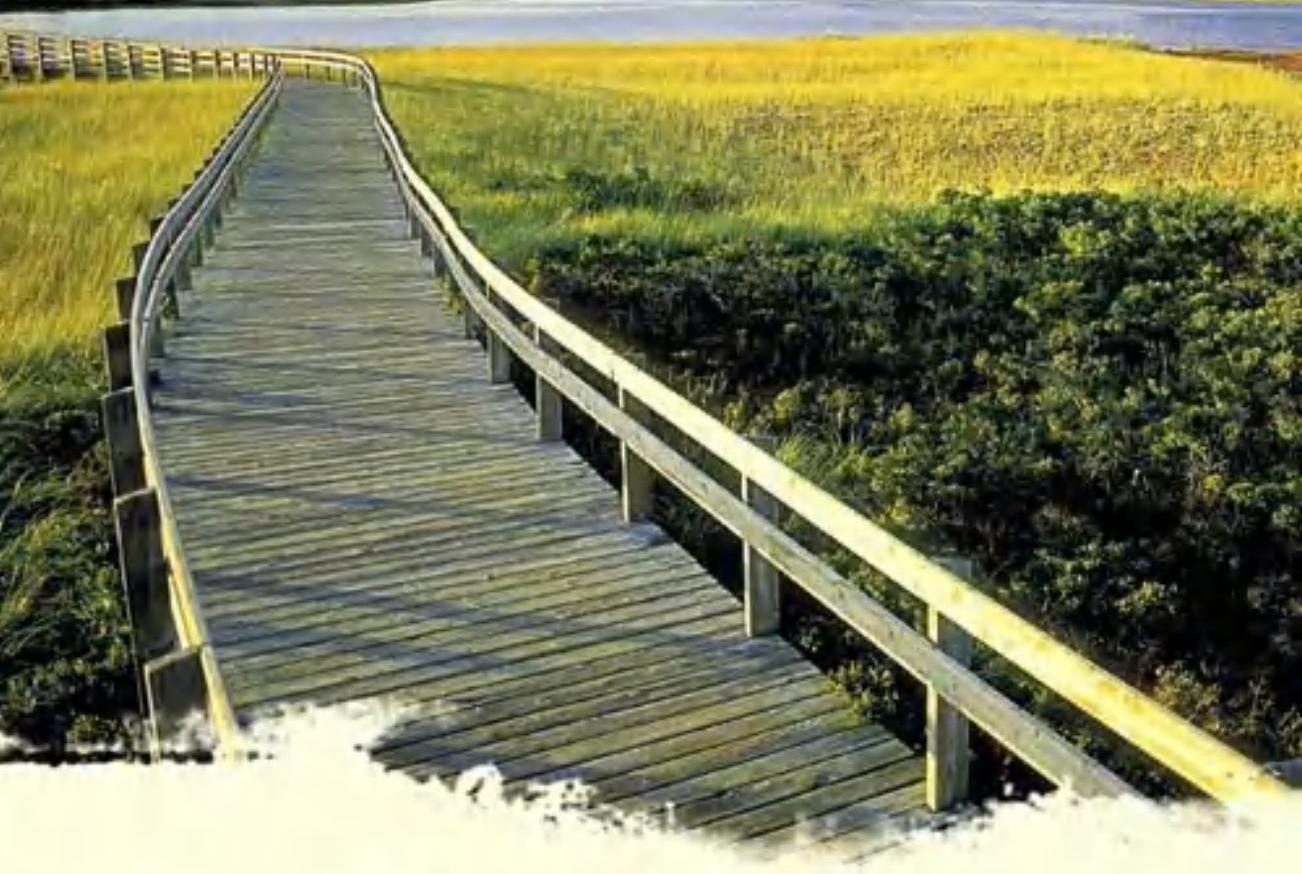
\includegraphics[max width=\textwidth, center]{2025_06_06_fac2836a92464059da43g-188}

听雨尘必@含 藏识\\
兔费越系来少下载


\end{document}